\chapter{DUNE long baseline analysis}
\label{sec:dune_lbl}

%%% Overall point of this chapter: How do our uncertainties relate to our ability to measure CPV
As covered in \citechap{sec:dune}, DUNE's primary goal is to make a measurement of CP violation (CPV) in the lepton sector.
Prior to any construction of the experiment, it is important to assess DUNE's eventual sensitivity to both CPV and other oscillation physics, such as the neutrino mass ordering.

\section{Summary of DUNE systematic uncertainties}
\label{sec:dune_lbl:systs}

This section gives a summary of the systematic uncertainties used in DUNE's long baseline analysis and where they are derived from.
\citesec{sec:dune_lbl:systs:flux} details the systematics deriving from lack of knowledge about the neutrino beam (commonly referred to as the `flux' systematics).
\citesec{sec:dune_lbl:systs:xsec} gives details of those systematics relating to lack of knowledge surrounding neutrino interactions with matter.
Finally, \citesec{sec:dune_lbl:systs:det} outlines the systematic uncertainties which derive from the uncertainty surrounding detector effects, for example the energy scale of the detector.

\subsection{Flux}
\label{sec:dune_lbl:systs:flux}

Uncertainties in the neutrino beam flux primarily arise from two sources: uncertainties in the production of hadrons by protons striking the beam target and uncertainties in the design parameters of the beam such as the horn currents or positioning (commonly referred to as the ``focussing uncertainties''.

The focussing uncertainties are evaluated by varying the beamline parameters within their tolerances and observing the resulting changes in the neutrino fluxes.
Hadron production uncertainties are estimated using uncertainties from thin target data experiments such as NA49~\cite{na49} with large uncertainties assigned to those interactions that are not covered by data.

\citefig{fig:fluxUncertainties} shows these uncertainties as a function of neutrino energy for the \numu and \anumu fluxes in both neutrino and antineutrino mode.
One can see that, at nearly all energies, hadron production uncertainties are larger than focussing uncertainties.

\begin{figure}[h]
  \centering
  \includegraphics[width=.8\linewidth]{files/figures/dune_detector/fluxUncertainties}
  \caption[Far detector flux uncertainties for \numu and \anumu]{Far detector \numu and \anumu flux uncertainties as a function of neutrino energy, from~\cite{tdrVol2}. The uncertainties are separated into those resulting from hadron production and those resulting from the focussing uncertainties.}
  \label{fig:fluxUncertainties}
\end{figure}

\subsection{Neutrino interaction (cross-section)}
\label{sec:dune_lbl:systs:xsec}

Uncertainties in the neutrino interaction model come from a variety of sources. 
The primary model used in the DUNE long-baseline analysis 

\subsection{Detector}
\label{sec:dune_lbl:systs:det}

Detector systematics in the DUNE long-baseline analysis primarily take the form of bin-to-bin shifts, rather than the weights typically used for the flux and cross-section systematics.
For various particle types there exist multi-parameter energy scale shifts of the form
\begin{equation}
E_{\alpha,~\text{reco}}' = E_{\alpha,~\text{reco}} \left( p_{0} + p_{1} \sqrt{E_{\alpha,~\text{reco}}} + \frac{p_{2}}{\sqrt{E_{\alpha,~\text{reco}}+0.1}} \right) \, ,
\label{eq:energyResponse}	
\end{equation}
where the $p_{n}$ are allowed to vary in any fits.
\citetab{tab:energyScaleParams} shows the $1\sigma$ values of the $p_{n}$ for each of the particle types.
All of these uncertainties are treated as uncorrelated between the near and far detectors.

The values of the $p_{0}$ (the absolute scale factors) are motivated by those values achieved in current long baseline neutrino experiments which use similar reconstruction techniques.
For example, the NOvA experiment quotes an absolute muon energy scale of $<1\%$ and a proton energy scale of 5\%~\cite{nova2018}.

\begin{table}
	\caption[$1\sigma$ uncertainties for the detector energy response used in the DUNE long baseline analysis]{$1\sigma$ uncertainties for the detector energy response used in the DUNE long baseline analysis. The muon curvature uncertainty only applies to those muons in the near detector which pass into the magnetised section of the detector.}
	\label{tab:energyScaleParams}
	\centering
	\begin{tabular}{c c c c}
		\hline
		\hline
		Particle types & \multicolumn{3}{c}{$1\sigma$ variation} \\
		& $p_{0}$ & $p_{1}$ & $p_{2}$ \\
		\hline
		All, except muons      & 2\%   & 1\%   & 2\%   \\
		$\mu$ (range)          & 2\%   & 2\%   & 2\%   \\
		$\mu$ (curvature)      & 1\%   & 1\%   & 1\%   \\
		$p$, \pipm             & 5\%   & 5\%   & 5\%   \\
		$e$, $\gamma$, \pizero & 2.5\% & 2.5\% & 2.5\% \\
		$n$                    & 20\%  & 30\%  & 30\% \\
		\hline
	\end{tabular}
\end{table}

\citefig{fig:protonEScale} shows 10 possible realisations of the proton energy response.
To produce each of these response functions, the $p_{n}$ are each independently thrown according to a Gaussian distribution with the appropriate width from \citetab{tab:energyScaleParams}.
One can see that between the different throws there are significant differences in both the magnitude and shape of response function between different throws.

\begin{figure}[h]
	\begin{adjustbox}{max totalsize=.6\textwidth, center}
		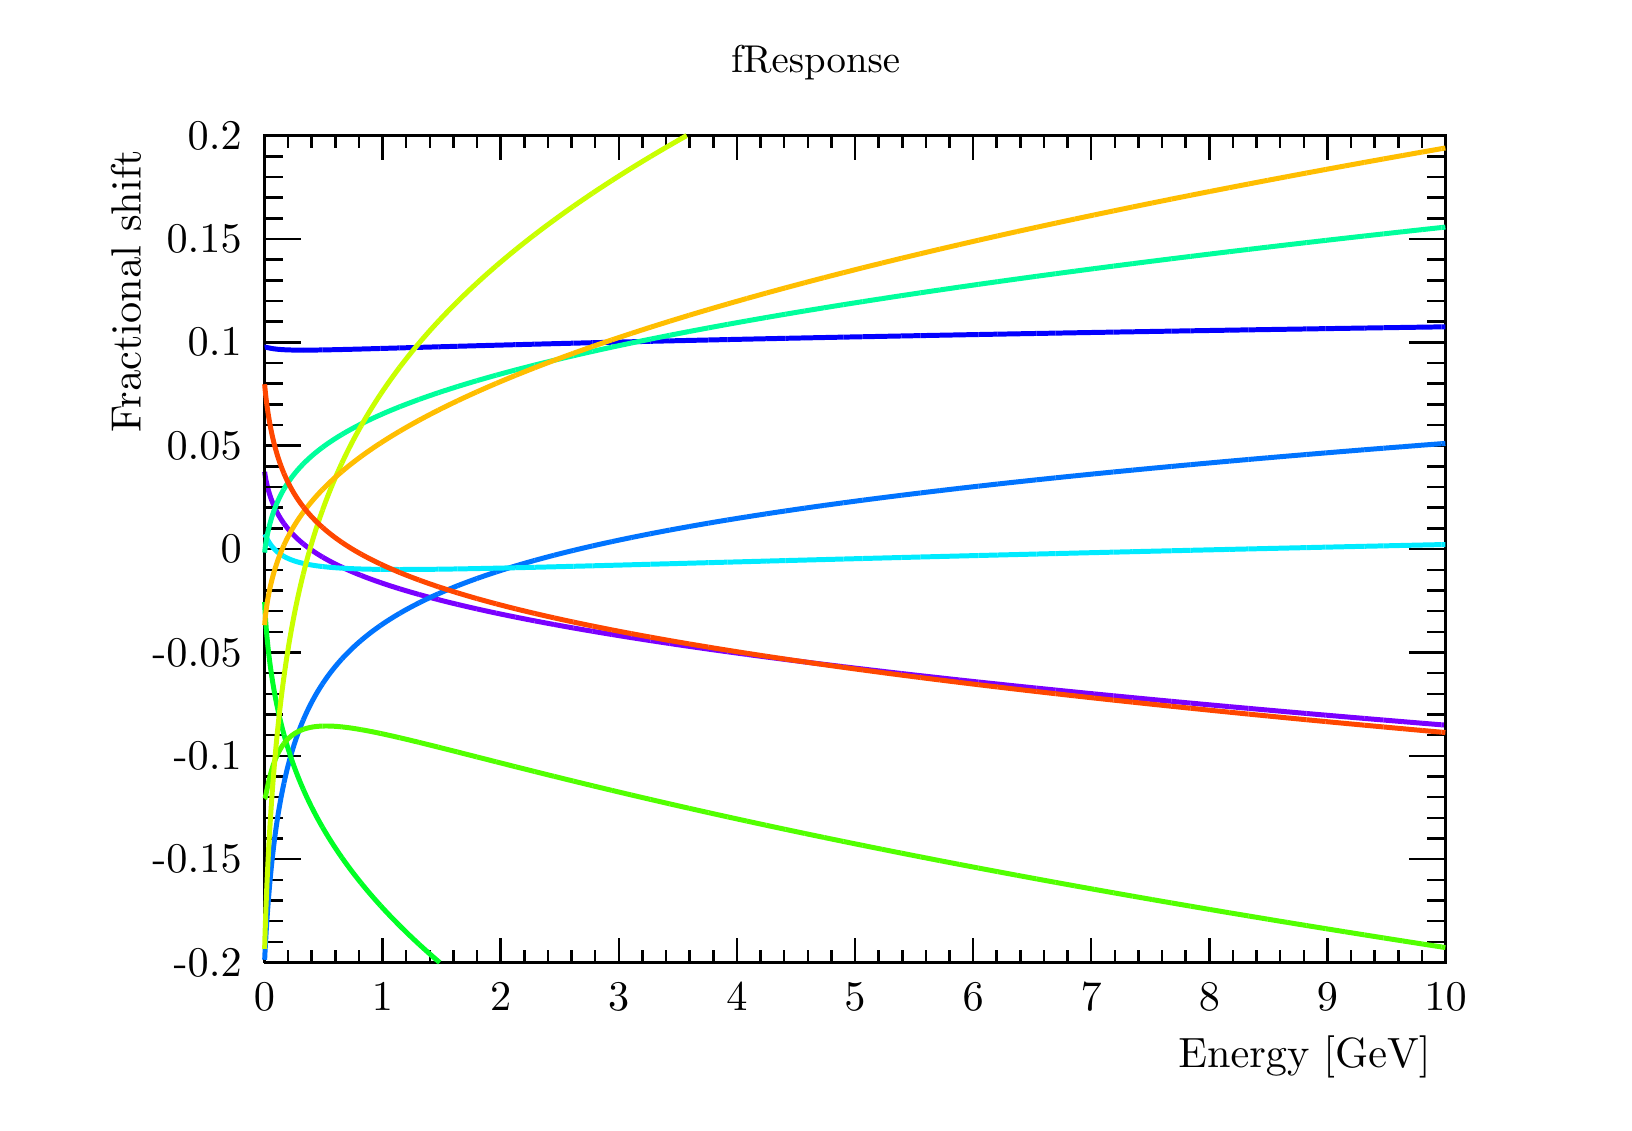
\begin{tikzpicture}
\pgfdeclareplotmark{cross} {
\pgfpathmoveto{\pgfpoint{-0.3\pgfplotmarksize}{\pgfplotmarksize}}
\pgfpathlineto{\pgfpoint{+0.3\pgfplotmarksize}{\pgfplotmarksize}}
\pgfpathlineto{\pgfpoint{+0.3\pgfplotmarksize}{0.3\pgfplotmarksize}}
\pgfpathlineto{\pgfpoint{+1\pgfplotmarksize}{0.3\pgfplotmarksize}}
\pgfpathlineto{\pgfpoint{+1\pgfplotmarksize}{-0.3\pgfplotmarksize}}
\pgfpathlineto{\pgfpoint{+0.3\pgfplotmarksize}{-0.3\pgfplotmarksize}}
\pgfpathlineto{\pgfpoint{+0.3\pgfplotmarksize}{-1.\pgfplotmarksize}}
\pgfpathlineto{\pgfpoint{-0.3\pgfplotmarksize}{-1.\pgfplotmarksize}}
\pgfpathlineto{\pgfpoint{-0.3\pgfplotmarksize}{-0.3\pgfplotmarksize}}
\pgfpathlineto{\pgfpoint{-1.\pgfplotmarksize}{-0.3\pgfplotmarksize}}
\pgfpathlineto{\pgfpoint{-1.\pgfplotmarksize}{0.3\pgfplotmarksize}}
\pgfpathlineto{\pgfpoint{-0.3\pgfplotmarksize}{0.3\pgfplotmarksize}}
\pgfpathclose
\pgfusepathqstroke
}
\pgfdeclareplotmark{cross*} {
\pgfpathmoveto{\pgfpoint{-0.3\pgfplotmarksize}{\pgfplotmarksize}}
\pgfpathlineto{\pgfpoint{+0.3\pgfplotmarksize}{\pgfplotmarksize}}
\pgfpathlineto{\pgfpoint{+0.3\pgfplotmarksize}{0.3\pgfplotmarksize}}
\pgfpathlineto{\pgfpoint{+1\pgfplotmarksize}{0.3\pgfplotmarksize}}
\pgfpathlineto{\pgfpoint{+1\pgfplotmarksize}{-0.3\pgfplotmarksize}}
\pgfpathlineto{\pgfpoint{+0.3\pgfplotmarksize}{-0.3\pgfplotmarksize}}
\pgfpathlineto{\pgfpoint{+0.3\pgfplotmarksize}{-1.\pgfplotmarksize}}
\pgfpathlineto{\pgfpoint{-0.3\pgfplotmarksize}{-1.\pgfplotmarksize}}
\pgfpathlineto{\pgfpoint{-0.3\pgfplotmarksize}{-0.3\pgfplotmarksize}}
\pgfpathlineto{\pgfpoint{-1.\pgfplotmarksize}{-0.3\pgfplotmarksize}}
\pgfpathlineto{\pgfpoint{-1.\pgfplotmarksize}{0.3\pgfplotmarksize}}
\pgfpathlineto{\pgfpoint{-0.3\pgfplotmarksize}{0.3\pgfplotmarksize}}
\pgfpathclose
\pgfusepathqfillstroke
}
\pgfdeclareplotmark{newstar} {
\pgfpathmoveto{\pgfqpoint{0pt}{\pgfplotmarksize}}
\pgfpathlineto{\pgfqpointpolar{44}{0.5\pgfplotmarksize}}
\pgfpathlineto{\pgfqpointpolar{18}{\pgfplotmarksize}}
\pgfpathlineto{\pgfqpointpolar{-20}{0.5\pgfplotmarksize}}
\pgfpathlineto{\pgfqpointpolar{-54}{\pgfplotmarksize}}
\pgfpathlineto{\pgfqpointpolar{-90}{0.5\pgfplotmarksize}}
\pgfpathlineto{\pgfqpointpolar{234}{\pgfplotmarksize}}
\pgfpathlineto{\pgfqpointpolar{198}{0.5\pgfplotmarksize}}
\pgfpathlineto{\pgfqpointpolar{162}{\pgfplotmarksize}}
\pgfpathlineto{\pgfqpointpolar{134}{0.5\pgfplotmarksize}}
\pgfpathclose
\pgfusepathqstroke
}
\pgfdeclareplotmark{newstar*} {
\pgfpathmoveto{\pgfqpoint{0pt}{\pgfplotmarksize}}
\pgfpathlineto{\pgfqpointpolar{44}{0.5\pgfplotmarksize}}
\pgfpathlineto{\pgfqpointpolar{18}{\pgfplotmarksize}}
\pgfpathlineto{\pgfqpointpolar{-20}{0.5\pgfplotmarksize}}
\pgfpathlineto{\pgfqpointpolar{-54}{\pgfplotmarksize}}
\pgfpathlineto{\pgfqpointpolar{-90}{0.5\pgfplotmarksize}}
\pgfpathlineto{\pgfqpointpolar{234}{\pgfplotmarksize}}
\pgfpathlineto{\pgfqpointpolar{198}{0.5\pgfplotmarksize}}
\pgfpathlineto{\pgfqpointpolar{162}{\pgfplotmarksize}}
\pgfpathlineto{\pgfqpointpolar{134}{0.5\pgfplotmarksize}}
\pgfpathclose
\pgfusepathqfillstroke
}
\definecolor{c}{rgb}{1,1,1};
\draw [color=c, fill=c] (0,0) rectangle (20,13.639);
\draw [color=c, fill=c] (3,1.77307) rectangle (18,12.2751);
\definecolor{c}{rgb}{0,0,0};
\draw [c,line width=0.9] (3,1.77307) -- (3,12.2751) -- (18,12.2751) -- (18,1.77307) -- (3,1.77307);
\definecolor{c}{rgb}{1,1,1};
\draw [color=c, fill=c] (3,1.77307) rectangle (18,12.2751);
\definecolor{c}{rgb}{0,0,0};
\draw [c,line width=0.9] (3,1.77307) -- (3,12.2751) -- (18,12.2751) -- (18,1.77307) -- (3,1.77307);
\definecolor{c}{rgb}{0.48,0,1};
\draw [c,line width=1.8] (3.0025,8.00548) -- (3.0075,7.96716) -- (3.0125,7.93646) -- (3.0175,7.9093) -- (3.0225,7.88446) -- (3.0275,7.86135) -- (3.0325,7.83965) -- (3.0375,7.81911) -- (3.0425,7.79958) -- (3.0475,7.78094) -- (3.0525,7.7631) --
 (3.0575,7.74598) -- (3.0625,7.7295) -- (3.0675,7.71363) -- (3.0725,7.69831) -- (3.0775,7.68351) -- (3.0825,7.66918) -- (3.0875,7.65529) -- (3.0925,7.64182) -- (3.0975,7.62875) -- (3.1025,7.61604) -- (3.1075,7.60368) -- (3.1125,7.59164) --
 (3.1175,7.57992) -- (3.1225,7.56849) -- (3.1275,7.55735) -- (3.1325,7.54647) -- (3.1375,7.53584) -- (3.1425,7.52545) -- (3.1475,7.5153) -- (3.1525,7.50537) -- (3.1575,7.49564) -- (3.1625,7.48612) -- (3.1675,7.4768) -- (3.1725,7.46766) --
 (3.1775,7.4587) -- (3.1825,7.44991) -- (3.1875,7.44129) -- (3.1925,7.43282) -- (3.1975,7.42451) -- (3.2025,7.41635) -- (3.2075,7.40832) -- (3.2125,7.40044) -- (3.2175,7.39269) -- (3.2225,7.38506) -- (3.2275,7.37756) -- (3.2325,7.37018) --
 (3.2375,7.36292) -- (3.2425,7.35577) -- (3.2475,7.34873);
\draw [c,line width=1.8] (3.2475,7.34873) -- (3.2525,7.34179) -- (3.2575,7.33495) -- (3.2625,7.32822) -- (3.2675,7.32157) -- (3.2725,7.31503) -- (3.2775,7.30857) -- (3.2825,7.3022) -- (3.2875,7.29592) -- (3.2925,7.28972) -- (3.2975,7.2836) --
 (3.3025,7.27756) -- (3.3075,7.2716) -- (3.3125,7.26571) -- (3.3175,7.2599) -- (3.3225,7.25415) -- (3.3275,7.24848) -- (3.3325,7.24287) -- (3.3375,7.23733) -- (3.3425,7.23185) -- (3.3475,7.22644) -- (3.3525,7.22108) -- (3.3575,7.21579) --
 (3.3625,7.21055) -- (3.3675,7.20537) -- (3.3725,7.20025) -- (3.3775,7.19518) -- (3.3825,7.19016) -- (3.3875,7.18519) -- (3.3925,7.18028) -- (3.3975,7.17542) -- (3.4025,7.1706) -- (3.4075,7.16583) -- (3.4125,7.16111) -- (3.4175,7.15643) --
 (3.4225,7.1518) -- (3.4275,7.14722) -- (3.4325,7.14267) -- (3.4375,7.13817) -- (3.4425,7.13371) -- (3.4475,7.12929) -- (3.4525,7.1249) -- (3.4575,7.12056) -- (3.4625,7.11626) -- (3.4675,7.11199) -- (3.4725,7.10776) -- (3.4775,7.10356) --
 (3.4825,7.0994) -- (3.4875,7.09528) -- (3.4925,7.09119);
\draw [c,line width=1.8] (3.4925,7.09119) -- (3.4975,7.08713) -- (3.5025,7.08311) -- (3.5075,7.07911) -- (3.5125,7.07515) -- (3.5175,7.07122) -- (3.5225,7.06733) -- (3.5275,7.06346) -- (3.5325,7.05962) -- (3.5375,7.05581) -- (3.5425,7.05202) --
 (3.5475,7.04827) -- (3.5525,7.04455) -- (3.5575,7.04085) -- (3.5625,7.03717) -- (3.5675,7.03353) -- (3.5725,7.02991) -- (3.5775,7.02631) -- (3.5825,7.02274) -- (3.5875,7.0192) -- (3.5925,7.01568) -- (3.5975,7.01218) -- (3.6025,7.00871) --
 (3.6075,7.00526) -- (3.6125,7.00183) -- (3.6175,6.99843) -- (3.6225,6.99505) -- (3.6275,6.99169) -- (3.6325,6.98835) -- (3.6375,6.98503) -- (3.6425,6.98173) -- (3.6475,6.97846) -- (3.6525,6.9752) -- (3.6575,6.97197) -- (3.6625,6.96875) --
 (3.6675,6.96556) -- (3.6725,6.96238) -- (3.6775,6.95922) -- (3.6825,6.95608) -- (3.6875,6.95296) -- (3.6925,6.94986) -- (3.6975,6.94677) -- (3.7025,6.94371) -- (3.7075,6.94066) -- (3.7125,6.93763) -- (3.7175,6.93461) -- (3.7225,6.93161) --
 (3.7275,6.92863) -- (3.7325,6.92567) -- (3.7375,6.92272);
\draw [c,line width=1.8] (3.7375,6.92272) -- (3.7425,6.91978) -- (3.7475,6.91687) -- (3.7525,6.91396) -- (3.7575,6.91108) -- (3.7625,6.90821) -- (3.7675,6.90535) -- (3.7725,6.90251) -- (3.7775,6.89968) -- (3.7825,6.89687) -- (3.7875,6.89407) --
 (3.7925,6.89129) -- (3.7975,6.88852) -- (3.8025,6.88576) -- (3.8075,6.88302) -- (3.8125,6.88029) -- (3.8175,6.87758) -- (3.8225,6.87488) -- (3.8275,6.87219) -- (3.8325,6.86951) -- (3.8375,6.86685) -- (3.8425,6.8642) -- (3.8475,6.86156) --
 (3.8525,6.85893) -- (3.8575,6.85632) -- (3.8625,6.85372) -- (3.8675,6.85113) -- (3.8725,6.84855) -- (3.8775,6.84598) -- (3.8825,6.84343) -- (3.8875,6.84088) -- (3.8925,6.83835) -- (3.8975,6.83583) -- (3.9025,6.83332) -- (3.9075,6.83082) --
 (3.9125,6.82833) -- (3.9175,6.82585) -- (3.9225,6.82339) -- (3.9275,6.82093) -- (3.9325,6.81848) -- (3.9375,6.81605) -- (3.9425,6.81362) -- (3.9475,6.81121) -- (3.9525,6.8088) -- (3.9575,6.80641) -- (3.9625,6.80402) -- (3.9675,6.80164) --
 (3.9725,6.79928) -- (3.9775,6.79692) -- (3.9825,6.79457);
\draw [c,line width=1.8] (3.9825,6.79457) -- (3.9875,6.79224) -- (3.9925,6.78991) -- (3.9975,6.78759) -- (4.0025,6.78528) -- (4.0075,6.78297) -- (4.0125,6.78068) -- (4.0175,6.7784) -- (4.0225,6.77612) -- (4.0275,6.77385) -- (4.0325,6.7716) --
 (4.0375,6.76935) -- (4.0425,6.76711) -- (4.0475,6.76487) -- (4.0525,6.76265) -- (4.0575,6.76043) -- (4.0625,6.75822) -- (4.0675,6.75602) -- (4.0725,6.75383) -- (4.0775,6.75165) -- (4.0825,6.74947) -- (4.0875,6.7473) -- (4.0925,6.74514) --
 (4.0975,6.74298) -- (4.1025,6.74084) -- (4.1075,6.7387) -- (4.1125,6.73657) -- (4.1175,6.73445) -- (4.1225,6.73233) -- (4.1275,6.73022) -- (4.1325,6.72812) -- (4.1375,6.72602) -- (4.1425,6.72393) -- (4.1475,6.72185) -- (4.1525,6.71978) --
 (4.1575,6.71771) -- (4.1625,6.71565) -- (4.1675,6.7136) -- (4.1725,6.71155) -- (4.1775,6.70951) -- (4.1825,6.70748) -- (4.1875,6.70545) -- (4.1925,6.70343) -- (4.1975,6.70142) -- (4.2025,6.69941) -- (4.2075,6.69741) -- (4.2125,6.69541) --
 (4.2175,6.69343) -- (4.2225,6.69144) -- (4.2275,6.68947);
\draw [c,line width=1.8] (4.2275,6.68947) -- (4.2325,6.6875) -- (4.2375,6.68553) -- (4.2425,6.68358) -- (4.2475,6.68162) -- (4.2525,6.67968) -- (4.2575,6.67774) -- (4.2625,6.6758) -- (4.2675,6.67387) -- (4.2725,6.67195) -- (4.2775,6.67003) --
 (4.2825,6.66812) -- (4.2875,6.66622) -- (4.2925,6.66432) -- (4.2975,6.66242) -- (4.3025,6.66053) -- (4.3075,6.65865) -- (4.3125,6.65677) -- (4.3175,6.6549) -- (4.3225,6.65303) -- (4.3275,6.65117) -- (4.3325,6.64931) -- (4.3375,6.64746) --
 (4.3425,6.64561) -- (4.3475,6.64377) -- (4.3525,6.64194) -- (4.3575,6.6401) -- (4.3625,6.63828) -- (4.3675,6.63646) -- (4.3725,6.63464) -- (4.3775,6.63283) -- (4.3825,6.63102) -- (4.3875,6.62922) -- (4.3925,6.62743) -- (4.3975,6.62563) --
 (4.4025,6.62385) -- (4.4075,6.62206) -- (4.4125,6.62029) -- (4.4175,6.61851) -- (4.4225,6.61675) -- (4.4275,6.61498) -- (4.4325,6.61322) -- (4.4375,6.61147) -- (4.4425,6.60972) -- (4.4475,6.60797) -- (4.4525,6.60623) -- (4.4575,6.6045) --
 (4.4625,6.60276) -- (4.4675,6.60104) -- (4.4725,6.59931);
\draw [c,line width=1.8] (4.4725,6.59931) -- (4.4775,6.59759) -- (4.4825,6.59588) -- (4.4875,6.59417) -- (4.4925,6.59246) -- (4.4975,6.59076) -- (4.5025,6.58906) -- (4.5075,6.58737) -- (4.5125,6.58568) -- (4.5175,6.58399) -- (4.5225,6.58231) --
 (4.5275,6.58064) -- (4.5325,6.57896) -- (4.5375,6.57729) -- (4.5425,6.57563) -- (4.5475,6.57397) -- (4.5525,6.57231) -- (4.5575,6.57066) -- (4.5625,6.56901) -- (4.5675,6.56736) -- (4.5725,6.56572) -- (4.5775,6.56408) -- (4.5825,6.56245) --
 (4.5875,6.56082) -- (4.5925,6.55919) -- (4.5975,6.55757) -- (4.6025,6.55595) -- (4.6075,6.55433) -- (4.6125,6.55272) -- (4.6175,6.55111) -- (4.6225,6.54951) -- (4.6275,6.54791) -- (4.6325,6.54631) -- (4.6375,6.54472) -- (4.6425,6.54313) --
 (4.6475,6.54154) -- (4.6525,6.53996) -- (4.6575,6.53838) -- (4.6625,6.5368) -- (4.6675,6.53523) -- (4.6725,6.53366) -- (4.6775,6.53209) -- (4.6825,6.53053) -- (4.6875,6.52897) -- (4.6925,6.52742) -- (4.6975,6.52586) -- (4.7025,6.52431) --
 (4.7075,6.52277) -- (4.7125,6.52122) -- (4.7175,6.51969);
\draw [c,line width=1.8] (4.7175,6.51969) -- (4.7225,6.51815) -- (4.7275,6.51662) -- (4.7325,6.51509) -- (4.7375,6.51356) -- (4.7425,6.51204) -- (4.7475,6.51052) -- (4.7525,6.509) -- (4.7575,6.50748) -- (4.7625,6.50597) -- (4.7675,6.50447) --
 (4.7725,6.50296) -- (4.7775,6.50146) -- (4.7825,6.49996) -- (4.7875,6.49846) -- (4.7925,6.49697) -- (4.7975,6.49548) -- (4.8025,6.494) -- (4.8075,6.49251) -- (4.8125,6.49103) -- (4.8175,6.48955) -- (4.8225,6.48808) -- (4.8275,6.48661) --
 (4.8325,6.48514) -- (4.8375,6.48367) -- (4.8425,6.48221) -- (4.8475,6.48075) -- (4.8525,6.47929) -- (4.8575,6.47783) -- (4.8625,6.47638) -- (4.8675,6.47493) -- (4.8725,6.47348) -- (4.8775,6.47204) -- (4.8825,6.4706) -- (4.8875,6.46916) --
 (4.8925,6.46772) -- (4.8975,6.46629) -- (4.9025,6.46486) -- (4.9075,6.46343) -- (4.9125,6.46201) -- (4.9175,6.46058) -- (4.9225,6.45917) -- (4.9275,6.45775) -- (4.9325,6.45633) -- (4.9375,6.45492) -- (4.9425,6.45351) -- (4.9475,6.4521) --
 (4.9525,6.4507) -- (4.9575,6.4493) -- (4.9625,6.4479);
\draw [c,line width=1.8] (4.9625,6.4479) -- (4.9675,6.4465) -- (4.9725,6.44511) -- (4.9775,6.44372) -- (4.9825,6.44233) -- (4.9875,6.44094) -- (4.9925,6.43956) -- (4.9975,6.43817) -- (5.0025,6.43679) -- (5.0075,6.43542) -- (5.0125,6.43404) --
 (5.0175,6.43267) -- (5.0225,6.4313) -- (5.0275,6.42993) -- (5.0325,6.42857) -- (5.0375,6.42721) -- (5.0425,6.42584) -- (5.0475,6.42449) -- (5.0525,6.42313) -- (5.0575,6.42178) -- (5.0625,6.42043) -- (5.0675,6.41908) -- (5.0725,6.41773) --
 (5.0775,6.41639) -- (5.0825,6.41504) -- (5.0875,6.4137) -- (5.0925,6.41237) -- (5.0975,6.41103) -- (5.1025,6.4097) -- (5.1075,6.40837) -- (5.1125,6.40704) -- (5.1175,6.40571) -- (5.1225,6.40439) -- (5.1275,6.40307) -- (5.1325,6.40175) --
 (5.1375,6.40043) -- (5.1425,6.39911) -- (5.1475,6.3978) -- (5.1525,6.39649) -- (5.1575,6.39518) -- (5.1625,6.39387) -- (5.1675,6.39257) -- (5.1725,6.39126) -- (5.1775,6.38996) -- (5.1825,6.38866) -- (5.1875,6.38737) -- (5.1925,6.38607) --
 (5.1975,6.38478) -- (5.2025,6.38349) -- (5.2075,6.3822);
\draw [c,line width=1.8] (5.2075,6.3822) -- (5.2125,6.38091) -- (5.2175,6.37963) -- (5.2225,6.37835) -- (5.2275,6.37707) -- (5.2325,6.37579) -- (5.2375,6.37451) -- (5.2425,6.37324) -- (5.2475,6.37196) -- (5.2525,6.37069) -- (5.2575,6.36942) --
 (5.2625,6.36816) -- (5.2675,6.36689) -- (5.2725,6.36563) -- (5.2775,6.36437) -- (5.2825,6.36311) -- (5.2875,6.36185) -- (5.2925,6.3606) -- (5.2975,6.35934) -- (5.3025,6.35809) -- (5.3075,6.35684) -- (5.3125,6.35559) -- (5.3175,6.35435) --
 (5.3225,6.3531) -- (5.3275,6.35186) -- (5.3325,6.35062) -- (5.3375,6.34938) -- (5.3425,6.34815) -- (5.3475,6.34691) -- (5.3525,6.34568) -- (5.3575,6.34445) -- (5.3625,6.34322) -- (5.3675,6.34199) -- (5.3725,6.34076) -- (5.3775,6.33954) --
 (5.3825,6.33832) -- (5.3875,6.3371) -- (5.3925,6.33588) -- (5.3975,6.33466) -- (5.4025,6.33344) -- (5.4075,6.33223) -- (5.4125,6.33102) -- (5.4175,6.32981) -- (5.4225,6.3286) -- (5.4275,6.32739) -- (5.4325,6.32619) -- (5.4375,6.32498) --
 (5.4425,6.32378) -- (5.4475,6.32258) -- (5.4525,6.32138);
\draw [c,line width=1.8] (5.4525,6.32138) -- (5.4575,6.32018) -- (5.4625,6.31899) -- (5.4675,6.3178) -- (5.4725,6.3166) -- (5.4775,6.31541) -- (5.4825,6.31422) -- (5.4875,6.31304) -- (5.4925,6.31185) -- (5.4975,6.31067) -- (5.5025,6.30949) --
 (5.5075,6.3083) -- (5.5125,6.30713) -- (5.5175,6.30595) -- (5.5225,6.30477) -- (5.5275,6.3036) -- (5.5325,6.30242) -- (5.5375,6.30125) -- (5.5425,6.30008) -- (5.5475,6.29892) -- (5.5525,6.29775) -- (5.5575,6.29658) -- (5.5625,6.29542) --
 (5.5675,6.29426) -- (5.5725,6.2931) -- (5.5775,6.29194) -- (5.5825,6.29078) -- (5.5875,6.28963) -- (5.5925,6.28847) -- (5.5975,6.28732) -- (5.6025,6.28617) -- (5.6075,6.28502) -- (5.6125,6.28387) -- (5.6175,6.28272) -- (5.6225,6.28158) --
 (5.6275,6.28043) -- (5.6325,6.27929) -- (5.6375,6.27815) -- (5.6425,6.27701) -- (5.6475,6.27587) -- (5.6525,6.27474) -- (5.6575,6.2736) -- (5.6625,6.27247) -- (5.6675,6.27133) -- (5.6725,6.2702) -- (5.6775,6.26907) -- (5.6825,6.26795) --
 (5.6875,6.26682) -- (5.6925,6.26569) -- (5.6975,6.26457);
\draw [c,line width=1.8] (5.6975,6.26457) -- (5.7025,6.26345) -- (5.7075,6.26233) -- (5.7125,6.26121) -- (5.7175,6.26009) -- (5.7225,6.25897) -- (5.7275,6.25785) -- (5.7325,6.25674) -- (5.7375,6.25563) -- (5.7425,6.25452) -- (5.7475,6.25341) --
 (5.7525,6.2523) -- (5.7575,6.25119) -- (5.7625,6.25008) -- (5.7675,6.24898) -- (5.7725,6.24788) -- (5.7775,6.24677) -- (5.7825,6.24567) -- (5.7875,6.24457) -- (5.7925,6.24347) -- (5.7975,6.24238) -- (5.8025,6.24128) -- (5.8075,6.24019) --
 (5.8125,6.23909) -- (5.8175,6.238) -- (5.8225,6.23691) -- (5.8275,6.23582) -- (5.8325,6.23474) -- (5.8375,6.23365) -- (5.8425,6.23256) -- (5.8475,6.23148) -- (5.8525,6.2304) -- (5.8575,6.22931) -- (5.8625,6.22823) -- (5.8675,6.22716) --
 (5.8725,6.22608) -- (5.8775,6.225) -- (5.8825,6.22393) -- (5.8875,6.22285) -- (5.8925,6.22178) -- (5.8975,6.22071) -- (5.9025,6.21964) -- (5.9075,6.21857) -- (5.9125,6.2175) -- (5.9175,6.21643) -- (5.9225,6.21537) -- (5.9275,6.2143) --
 (5.9325,6.21324) -- (5.9375,6.21218) -- (5.9425,6.21112);
\draw [c,line width=1.8] (5.9425,6.21112) -- (5.9475,6.21006) -- (5.9525,6.209) -- (5.9575,6.20794) -- (5.9625,6.20689) -- (5.9675,6.20583) -- (5.9725,6.20478) -- (5.9775,6.20372) -- (5.9825,6.20267) -- (5.9875,6.20162) -- (5.9925,6.20057) --
 (5.9975,6.19953) -- (6.0025,6.19848) -- (6.0075,6.19743) -- (6.0125,6.19639) -- (6.0175,6.19535) -- (6.0225,6.1943) -- (6.0275,6.19326) -- (6.0325,6.19222) -- (6.0375,6.19118) -- (6.0425,6.19015) -- (6.0475,6.18911) -- (6.0525,6.18807) --
 (6.0575,6.18704) -- (6.0625,6.18601) -- (6.0675,6.18497) -- (6.0725,6.18394) -- (6.0775,6.18291) -- (6.0825,6.18188) -- (6.0875,6.18086) -- (6.0925,6.17983) -- (6.0975,6.1788) -- (6.1025,6.17778) -- (6.1075,6.17676) -- (6.1125,6.17573) --
 (6.1175,6.17471) -- (6.1225,6.17369) -- (6.1275,6.17267) -- (6.1325,6.17166) -- (6.1375,6.17064) -- (6.1425,6.16962) -- (6.1475,6.16861) -- (6.1525,6.16759) -- (6.1575,6.16658) -- (6.1625,6.16557) -- (6.1675,6.16456) -- (6.1725,6.16355) --
 (6.1775,6.16254) -- (6.1825,6.16153) -- (6.1875,6.16053);
\draw [c,line width=1.8] (6.1875,6.16053) -- (6.1925,6.15952) -- (6.1975,6.15852) -- (6.2025,6.15751) -- (6.2075,6.15651) -- (6.2125,6.15551) -- (6.2175,6.15451) -- (6.2225,6.15351) -- (6.2275,6.15251) -- (6.2325,6.15151) -- (6.2375,6.15052) --
 (6.2425,6.14952) -- (6.2475,6.14853) -- (6.2525,6.14753) -- (6.2575,6.14654) -- (6.2625,6.14555) -- (6.2675,6.14456) -- (6.2725,6.14357) -- (6.2775,6.14258) -- (6.2825,6.14159) -- (6.2875,6.14061) -- (6.2925,6.13962) -- (6.2975,6.13864) --
 (6.3025,6.13765) -- (6.3075,6.13667) -- (6.3125,6.13569) -- (6.3175,6.13471) -- (6.3225,6.13373) -- (6.3275,6.13275) -- (6.3325,6.13177) -- (6.3375,6.1308) -- (6.3425,6.12982) -- (6.3475,6.12884) -- (6.3525,6.12787) -- (6.3575,6.1269) --
 (6.3625,6.12593) -- (6.3675,6.12495) -- (6.3725,6.12398) -- (6.3775,6.12301) -- (6.3825,6.12205) -- (6.3875,6.12108) -- (6.3925,6.12011) -- (6.3975,6.11915) -- (6.4025,6.11818) -- (6.4075,6.11722) -- (6.4125,6.11625) -- (6.4175,6.11529) --
 (6.4225,6.11433) -- (6.4275,6.11337) -- (6.4325,6.11241);
\draw [c,line width=1.8] (6.4325,6.11241) -- (6.4375,6.11145) -- (6.4425,6.11049) -- (6.4475,6.10954) -- (6.4525,6.10858) -- (6.4575,6.10763) -- (6.4625,6.10667) -- (6.4675,6.10572) -- (6.4725,6.10477) -- (6.4775,6.10382) -- (6.4825,6.10287) --
 (6.4875,6.10192) -- (6.4925,6.10097) -- (6.4975,6.10002) -- (6.5025,6.09907) -- (6.5075,6.09813) -- (6.5125,6.09718) -- (6.5175,6.09624) -- (6.5225,6.09529) -- (6.5275,6.09435) -- (6.5325,6.09341) -- (6.5375,6.09247) -- (6.5425,6.09153) --
 (6.5475,6.09059) -- (6.5525,6.08965) -- (6.5575,6.08871) -- (6.5625,6.08777) -- (6.5675,6.08684) -- (6.5725,6.0859) -- (6.5775,6.08497) -- (6.5825,6.08404) -- (6.5875,6.0831) -- (6.5925,6.08217) -- (6.5975,6.08124) -- (6.6025,6.08031) --
 (6.6075,6.07938) -- (6.6125,6.07845) -- (6.6175,6.07752) -- (6.6225,6.0766) -- (6.6275,6.07567) -- (6.6325,6.07475) -- (6.6375,6.07382) -- (6.6425,6.0729) -- (6.6475,6.07198) -- (6.6525,6.07105) -- (6.6575,6.07013) -- (6.6625,6.06921) --
 (6.6675,6.06829) -- (6.6725,6.06737) -- (6.6775,6.06646);
\draw [c,line width=1.8] (6.6775,6.06646) -- (6.6825,6.06554) -- (6.6875,6.06462) -- (6.6925,6.06371) -- (6.6975,6.06279) -- (6.7025,6.06188) -- (6.7075,6.06096) -- (6.7125,6.06005) -- (6.7175,6.05914) -- (6.7225,6.05823) -- (6.7275,6.05732) --
 (6.7325,6.05641) -- (6.7375,6.0555) -- (6.7425,6.05459) -- (6.7475,6.05369) -- (6.7525,6.05278) -- (6.7575,6.05187) -- (6.7625,6.05097) -- (6.7675,6.05007) -- (6.7725,6.04916) -- (6.7775,6.04826) -- (6.7825,6.04736) -- (6.7875,6.04646) --
 (6.7925,6.04556) -- (6.7975,6.04466) -- (6.8025,6.04376) -- (6.8075,6.04286) -- (6.8125,6.04196) -- (6.8175,6.04107) -- (6.8225,6.04017) -- (6.8275,6.03928) -- (6.8325,6.03838) -- (6.8375,6.03749) -- (6.8425,6.0366) -- (6.8475,6.0357) --
 (6.8525,6.03481) -- (6.8575,6.03392) -- (6.8625,6.03303) -- (6.8675,6.03214) -- (6.8725,6.03125) -- (6.8775,6.03037) -- (6.8825,6.02948) -- (6.8875,6.02859) -- (6.8925,6.02771) -- (6.8975,6.02682) -- (6.9025,6.02594) -- (6.9075,6.02506) --
 (6.9125,6.02417) -- (6.9175,6.02329) -- (6.9225,6.02241);
\draw [c,line width=1.8] (6.9225,6.02241) -- (6.9275,6.02153) -- (6.9325,6.02065) -- (6.9375,6.01977) -- (6.9425,6.01889) -- (6.9475,6.01801) -- (6.9525,6.01714) -- (6.9575,6.01626) -- (6.9625,6.01539) -- (6.9675,6.01451) -- (6.9725,6.01364) --
 (6.9775,6.01276) -- (6.9825,6.01189) -- (6.9875,6.01102) -- (6.9925,6.01015) -- (6.9975,6.00928) -- (7.0025,6.00841) -- (7.0075,6.00754) -- (7.0125,6.00667) -- (7.0175,6.0058) -- (7.0225,6.00493) -- (7.0275,6.00406) -- (7.0325,6.0032) --
 (7.0375,6.00233) -- (7.0425,6.00147) -- (7.0475,6.0006) -- (7.0525,5.99974) -- (7.0575,5.99888) -- (7.0625,5.99802) -- (7.0675,5.99716) -- (7.0725,5.99629) -- (7.0775,5.99543) -- (7.0825,5.99458) -- (7.0875,5.99372) -- (7.0925,5.99286) --
 (7.0975,5.992) -- (7.1025,5.99114) -- (7.1075,5.99029) -- (7.1125,5.98943) -- (7.1175,5.98858) -- (7.1225,5.98772) -- (7.1275,5.98687) -- (7.1325,5.98602) -- (7.1375,5.98516) -- (7.1425,5.98431) -- (7.1475,5.98346) -- (7.1525,5.98261) --
 (7.1575,5.98176) -- (7.1625,5.98091) -- (7.1675,5.98006);
\draw [c,line width=1.8] (7.1675,5.98006) -- (7.1725,5.97922) -- (7.1775,5.97837) -- (7.1825,5.97752) -- (7.1875,5.97668) -- (7.1925,5.97583) -- (7.1975,5.97499) -- (7.2025,5.97414) -- (7.2075,5.9733) -- (7.2125,5.97246) -- (7.2175,5.97162) --
 (7.2225,5.97077) -- (7.2275,5.96993) -- (7.2325,5.96909) -- (7.2375,5.96825) -- (7.2425,5.96741) -- (7.2475,5.96658) -- (7.2525,5.96574) -- (7.2575,5.9649) -- (7.2625,5.96406) -- (7.2675,5.96323) -- (7.2725,5.96239) -- (7.2775,5.96156) --
 (7.2825,5.96072) -- (7.2875,5.95989) -- (7.2925,5.95906) -- (7.2975,5.95823) -- (7.3025,5.95739) -- (7.3075,5.95656) -- (7.3125,5.95573) -- (7.3175,5.9549) -- (7.3225,5.95407) -- (7.3275,5.95324) -- (7.3325,5.95242) -- (7.3375,5.95159) --
 (7.3425,5.95076) -- (7.3475,5.94994) -- (7.3525,5.94911) -- (7.3575,5.94828) -- (7.3625,5.94746) -- (7.3675,5.94664) -- (7.3725,5.94581) -- (7.3775,5.94499) -- (7.3825,5.94417) -- (7.3875,5.94335) -- (7.3925,5.94252) -- (7.3975,5.9417) --
 (7.4025,5.94088) -- (7.4075,5.94006) -- (7.4125,5.93925);
\draw [c,line width=1.8] (7.4125,5.93925) -- (7.4175,5.93843) -- (7.4225,5.93761) -- (7.4275,5.93679) -- (7.4325,5.93598) -- (7.4375,5.93516) -- (7.4425,5.93434) -- (7.4475,5.93353) -- (7.4525,5.93272) -- (7.4575,5.9319) -- (7.4625,5.93109) --
 (7.4675,5.93028) -- (7.4725,5.92946) -- (7.4775,5.92865) -- (7.4825,5.92784) -- (7.4875,5.92703) -- (7.4925,5.92622) -- (7.4975,5.92541) -- (7.5025,5.9246) -- (7.5075,5.9238) -- (7.5125,5.92299) -- (7.5175,5.92218) -- (7.5225,5.92138) --
 (7.5275,5.92057) -- (7.5325,5.91976) -- (7.5375,5.91896) -- (7.5425,5.91815) -- (7.5475,5.91735) -- (7.5525,5.91655) -- (7.5575,5.91575) -- (7.5625,5.91494) -- (7.5675,5.91414) -- (7.5725,5.91334) -- (7.5775,5.91254) -- (7.5825,5.91174) --
 (7.5875,5.91094) -- (7.5925,5.91014) -- (7.5975,5.90934) -- (7.6025,5.90855) -- (7.6075,5.90775) -- (7.6125,5.90695) -- (7.6175,5.90616) -- (7.6225,5.90536) -- (7.6275,5.90457) -- (7.6325,5.90377) -- (7.6375,5.90298) -- (7.6425,5.90218) --
 (7.6475,5.90139) -- (7.6525,5.9006) -- (7.6575,5.89981);
\draw [c,line width=1.8] (7.6575,5.89981) -- (7.6625,5.89901) -- (7.6675,5.89822) -- (7.6725,5.89743) -- (7.6775,5.89664) -- (7.6825,5.89585) -- (7.6875,5.89506) -- (7.6925,5.89428) -- (7.6975,5.89349) -- (7.7025,5.8927) -- (7.7075,5.89191) --
 (7.7125,5.89113) -- (7.7175,5.89034) -- (7.7225,5.88956) -- (7.7275,5.88877) -- (7.7325,5.88799) -- (7.7375,5.8872) -- (7.7425,5.88642) -- (7.7475,5.88564) -- (7.7525,5.88486) -- (7.7575,5.88407) -- (7.7625,5.88329) -- (7.7675,5.88251) --
 (7.7725,5.88173) -- (7.7775,5.88095) -- (7.7825,5.88017) -- (7.7875,5.87939) -- (7.7925,5.87862) -- (7.7975,5.87784) -- (7.8025,5.87706) -- (7.8075,5.87628) -- (7.8125,5.87551) -- (7.8175,5.87473) -- (7.8225,5.87396) -- (7.8275,5.87318) --
 (7.8325,5.87241) -- (7.8375,5.87163) -- (7.8425,5.87086) -- (7.8475,5.87009) -- (7.8525,5.86932) -- (7.8575,5.86854) -- (7.8625,5.86777) -- (7.8675,5.867) -- (7.8725,5.86623) -- (7.8775,5.86546) -- (7.8825,5.86469) -- (7.8875,5.86392) --
 (7.8925,5.86315) -- (7.8975,5.86239) -- (7.9025,5.86162);
\draw [c,line width=1.8] (7.9025,5.86162) -- (7.9075,5.86085) -- (7.9125,5.86009) -- (7.9175,5.85932) -- (7.9225,5.85855) -- (7.9275,5.85779) -- (7.9325,5.85702) -- (7.9375,5.85626) -- (7.9425,5.8555) -- (7.9475,5.85473) -- (7.9525,5.85397) --
 (7.9575,5.85321) -- (7.9625,5.85245) -- (7.9675,5.85168) -- (7.9725,5.85092) -- (7.9775,5.85016) -- (7.9825,5.8494) -- (7.9875,5.84864) -- (7.9925,5.84788) -- (7.9975,5.84713) -- (8.0025,5.84637) -- (8.0075,5.84561) -- (8.0125,5.84485) --
 (8.0175,5.8441) -- (8.0225,5.84334) -- (8.0275,5.84258) -- (8.0325,5.84183) -- (8.0375,5.84107) -- (8.0425,5.84032) -- (8.0475,5.83956) -- (8.0525,5.83881) -- (8.0575,5.83806) -- (8.0625,5.8373) -- (8.0675,5.83655) -- (8.0725,5.8358) --
 (8.0775,5.83505) -- (8.0825,5.8343) -- (8.0875,5.83355) -- (8.0925,5.8328) -- (8.0975,5.83205) -- (8.1025,5.8313) -- (8.1075,5.83055) -- (8.1125,5.8298) -- (8.1175,5.82905) -- (8.1225,5.82831) -- (8.1275,5.82756) -- (8.1325,5.82681) --
 (8.1375,5.82607) -- (8.1425,5.82532) -- (8.1475,5.82458);
\draw [c,line width=1.8] (8.1475,5.82458) -- (8.1525,5.82383) -- (8.1575,5.82309) -- (8.1625,5.82234) -- (8.1675,5.8216) -- (8.1725,5.82086) -- (8.1775,5.82012) -- (8.1825,5.81937) -- (8.1875,5.81863) -- (8.1925,5.81789) -- (8.1975,5.81715) --
 (8.2025,5.81641) -- (8.2075,5.81567) -- (8.2125,5.81493) -- (8.2175,5.81419) -- (8.2225,5.81345) -- (8.2275,5.81271) -- (8.2325,5.81198) -- (8.2375,5.81124) -- (8.2425,5.8105) -- (8.2475,5.80977) -- (8.2525,5.80903) -- (8.2575,5.80829) --
 (8.2625,5.80756) -- (8.2675,5.80682) -- (8.2725,5.80609) -- (8.2775,5.80536) -- (8.2825,5.80462) -- (8.2875,5.80389) -- (8.2925,5.80316) -- (8.2975,5.80242) -- (8.3025,5.80169) -- (8.3075,5.80096) -- (8.3125,5.80023) -- (8.3175,5.7995) --
 (8.3225,5.79877) -- (8.3275,5.79804) -- (8.3325,5.79731) -- (8.3375,5.79658) -- (8.3425,5.79585) -- (8.3475,5.79512) -- (8.3525,5.79439) -- (8.3575,5.79367) -- (8.3625,5.79294) -- (8.3675,5.79221) -- (8.3725,5.79149) -- (8.3775,5.79076) --
 (8.3825,5.79004) -- (8.3875,5.78931) -- (8.3925,5.78859);
\draw [c,line width=1.8] (8.3925,5.78859) -- (8.3975,5.78786) -- (8.4025,5.78714) -- (8.4075,5.78642) -- (8.4125,5.78569) -- (8.4175,5.78497) -- (8.4225,5.78425) -- (8.4275,5.78353) -- (8.4325,5.78281) -- (8.4375,5.78208) -- (8.4425,5.78136) --
 (8.4475,5.78064) -- (8.4525,5.77992) -- (8.4575,5.7792) -- (8.4625,5.77849) -- (8.4675,5.77777) -- (8.4725,5.77705) -- (8.4775,5.77633) -- (8.4825,5.77561) -- (8.4875,5.7749) -- (8.4925,5.77418) -- (8.4975,5.77346) -- (8.5025,5.77275) --
 (8.5075,5.77203) -- (8.5125,5.77132) -- (8.5175,5.7706) -- (8.5225,5.76989) -- (8.5275,5.76918) -- (8.5325,5.76846) -- (8.5375,5.76775) -- (8.5425,5.76704) -- (8.5475,5.76632) -- (8.5525,5.76561) -- (8.5575,5.7649) -- (8.5625,5.76419) --
 (8.5675,5.76348) -- (8.5725,5.76277) -- (8.5775,5.76206) -- (8.5825,5.76135) -- (8.5875,5.76064) -- (8.5925,5.75993) -- (8.5975,5.75922) -- (8.6025,5.75851) -- (8.6075,5.75781) -- (8.6125,5.7571) -- (8.6175,5.75639) -- (8.6225,5.75568) --
 (8.6275,5.75498) -- (8.6325,5.75427) -- (8.6375,5.75357);
\draw [c,line width=1.8] (8.6375,5.75357) -- (8.6425,5.75286) -- (8.6475,5.75216) -- (8.6525,5.75145) -- (8.6575,5.75075) -- (8.6625,5.75005) -- (8.6675,5.74934) -- (8.6725,5.74864) -- (8.6775,5.74794) -- (8.6825,5.74723) -- (8.6875,5.74653) --
 (8.6925,5.74583) -- (8.6975,5.74513) -- (8.7025,5.74443) -- (8.7075,5.74373) -- (8.7125,5.74303) -- (8.7175,5.74233) -- (8.7225,5.74163) -- (8.7275,5.74093) -- (8.7325,5.74023) -- (8.7375,5.73953) -- (8.7425,5.73884) -- (8.7475,5.73814) --
 (8.7525,5.73744) -- (8.7575,5.73675) -- (8.7625,5.73605) -- (8.7675,5.73535) -- (8.7725,5.73466) -- (8.7775,5.73396) -- (8.7825,5.73327) -- (8.7875,5.73257) -- (8.7925,5.73188) -- (8.7975,5.73119) -- (8.8025,5.73049) -- (8.8075,5.7298) --
 (8.8125,5.72911) -- (8.8175,5.72841) -- (8.8225,5.72772) -- (8.8275,5.72703) -- (8.8325,5.72634) -- (8.8375,5.72565) -- (8.8425,5.72496) -- (8.8475,5.72427) -- (8.8525,5.72358) -- (8.8575,5.72289) -- (8.8625,5.7222) -- (8.8675,5.72151) --
 (8.8725,5.72082) -- (8.8775,5.72013) -- (8.8825,5.71944);
\draw [c,line width=1.8] (8.8825,5.71944) -- (8.8875,5.71876) -- (8.8925,5.71807) -- (8.8975,5.71738) -- (8.9025,5.7167) -- (8.9075,5.71601) -- (8.9125,5.71532) -- (8.9175,5.71464) -- (8.9225,5.71395) -- (8.9275,5.71327) -- (8.9325,5.71258) --
 (8.9375,5.7119) -- (8.9425,5.71122) -- (8.9475,5.71053) -- (8.9525,5.70985) -- (8.9575,5.70917) -- (8.9625,5.70849) -- (8.9675,5.7078) -- (8.9725,5.70712) -- (8.9775,5.70644) -- (8.9825,5.70576) -- (8.9875,5.70508) -- (8.9925,5.7044) --
 (8.9975,5.70372) -- (9.0025,5.70304) -- (9.0075,5.70236) -- (9.0125,5.70168) -- (9.0175,5.701) -- (9.0225,5.70032) -- (9.0275,5.69965) -- (9.0325,5.69897) -- (9.0375,5.69829) -- (9.0425,5.69761) -- (9.0475,5.69694) -- (9.0525,5.69626) --
 (9.0575,5.69559) -- (9.0625,5.69491) -- (9.0675,5.69423) -- (9.0725,5.69356) -- (9.0775,5.69288) -- (9.0825,5.69221) -- (9.0875,5.69154) -- (9.0925,5.69086) -- (9.0975,5.69019) -- (9.1025,5.68952) -- (9.1075,5.68884) -- (9.1125,5.68817) --
 (9.1175,5.6875) -- (9.1225,5.68683) -- (9.1275,5.68616);
\draw [c,line width=1.8] (9.1275,5.68616) -- (9.1325,5.68548) -- (9.1375,5.68481) -- (9.1425,5.68414) -- (9.1475,5.68347) -- (9.1525,5.6828) -- (9.1575,5.68213) -- (9.1625,5.68147) -- (9.1675,5.6808) -- (9.1725,5.68013) -- (9.1775,5.67946) --
 (9.1825,5.67879) -- (9.1875,5.67812) -- (9.1925,5.67746) -- (9.1975,5.67679) -- (9.2025,5.67612) -- (9.2075,5.67546) -- (9.2125,5.67479) -- (9.2175,5.67413) -- (9.2225,5.67346) -- (9.2275,5.6728) -- (9.2325,5.67213) -- (9.2375,5.67147) --
 (9.2425,5.6708) -- (9.2475,5.67014) -- (9.2525,5.66948) -- (9.2575,5.66881) -- (9.2625,5.66815) -- (9.2675,5.66749) -- (9.2725,5.66682) -- (9.2775,5.66616) -- (9.2825,5.6655) -- (9.2875,5.66484) -- (9.2925,5.66418) -- (9.2975,5.66352) --
 (9.3025,5.66286) -- (9.3075,5.6622) -- (9.3125,5.66154) -- (9.3175,5.66088) -- (9.3225,5.66022) -- (9.3275,5.65956) -- (9.3325,5.6589) -- (9.3375,5.65824) -- (9.3425,5.65759) -- (9.3475,5.65693) -- (9.3525,5.65627) -- (9.3575,5.65561) --
 (9.3625,5.65496) -- (9.3675,5.6543) -- (9.3725,5.65365);
\draw [c,line width=1.8] (9.3725,5.65365) -- (9.3775,5.65299) -- (9.3825,5.65233) -- (9.3875,5.65168) -- (9.3925,5.65102) -- (9.3975,5.65037) -- (9.4025,5.64971) -- (9.4075,5.64906) -- (9.4125,5.64841) -- (9.4175,5.64775) -- (9.4225,5.6471) --
 (9.4275,5.64645) -- (9.4325,5.6458) -- (9.4375,5.64514) -- (9.4425,5.64449) -- (9.4475,5.64384) -- (9.4525,5.64319) -- (9.4575,5.64254) -- (9.4625,5.64189) -- (9.4675,5.64124) -- (9.4725,5.64059) -- (9.4775,5.63994) -- (9.4825,5.63929) --
 (9.4875,5.63864) -- (9.4925,5.63799) -- (9.4975,5.63734) -- (9.5025,5.63669) -- (9.5075,5.63604) -- (9.5125,5.6354) -- (9.5175,5.63475) -- (9.5225,5.6341) -- (9.5275,5.63346) -- (9.5325,5.63281) -- (9.5375,5.63216) -- (9.5425,5.63152) --
 (9.5475,5.63087) -- (9.5525,5.63023) -- (9.5575,5.62958) -- (9.5625,5.62893) -- (9.5675,5.62829) -- (9.5725,5.62765) -- (9.5775,5.627) -- (9.5825,5.62636) -- (9.5875,5.62572) -- (9.5925,5.62507) -- (9.5975,5.62443) -- (9.6025,5.62379) --
 (9.6075,5.62314) -- (9.6125,5.6225) -- (9.6175,5.62186);
\draw [c,line width=1.8] (9.6175,5.62186) -- (9.6225,5.62122) -- (9.6275,5.62058) -- (9.6325,5.61994) -- (9.6375,5.6193) -- (9.6425,5.61866) -- (9.6475,5.61802) -- (9.6525,5.61738) -- (9.6575,5.61674) -- (9.6625,5.6161) -- (9.6675,5.61546) --
 (9.6725,5.61482) -- (9.6775,5.61418) -- (9.6825,5.61354) -- (9.6875,5.61291) -- (9.6925,5.61227) -- (9.6975,5.61163) -- (9.7025,5.61099) -- (9.7075,5.61036) -- (9.7125,5.60972) -- (9.7175,5.60909) -- (9.7225,5.60845) -- (9.7275,5.60781) --
 (9.7325,5.60718) -- (9.7375,5.60654) -- (9.7425,5.60591) -- (9.7475,5.60527) -- (9.7525,5.60464) -- (9.7575,5.60401) -- (9.7625,5.60337) -- (9.7675,5.60274) -- (9.7725,5.60211) -- (9.7775,5.60147) -- (9.7825,5.60084) -- (9.7875,5.60021) --
 (9.7925,5.59958) -- (9.7975,5.59895) -- (9.8025,5.59831) -- (9.8075,5.59768) -- (9.8125,5.59705) -- (9.8175,5.59642) -- (9.8225,5.59579) -- (9.8275,5.59516) -- (9.8325,5.59453) -- (9.8375,5.5939) -- (9.8425,5.59327) -- (9.8475,5.59264) --
 (9.8525,5.59201) -- (9.8575,5.59139) -- (9.8625,5.59076);
\draw [c,line width=1.8] (9.8625,5.59076) -- (9.8675,5.59013) -- (9.8725,5.5895) -- (9.8775,5.58887) -- (9.8825,5.58825) -- (9.8875,5.58762) -- (9.8925,5.58699) -- (9.8975,5.58637) -- (9.9025,5.58574) -- (9.9075,5.58512) -- (9.9125,5.58449) --
 (9.9175,5.58386) -- (9.9225,5.58324) -- (9.9275,5.58261) -- (9.9325,5.58199) -- (9.9375,5.58137) -- (9.9425,5.58074) -- (9.9475,5.58012) -- (9.9525,5.57949) -- (9.9575,5.57887) -- (9.9625,5.57825) -- (9.9675,5.57763) -- (9.9725,5.577) --
 (9.9775,5.57638) -- (9.9825,5.57576) -- (9.9875,5.57514) -- (9.9925,5.57452) -- (9.9975,5.57389) -- (10.0025,5.57327) -- (10.0075,5.57265) -- (10.0125,5.57203) -- (10.0175,5.57141) -- (10.0225,5.57079) -- (10.0275,5.57017) -- (10.0325,5.56955) --
 (10.0375,5.56894) -- (10.0425,5.56832) -- (10.0475,5.5677) -- (10.0525,5.56708) -- (10.0575,5.56646) -- (10.0625,5.56584) -- (10.0675,5.56523) -- (10.0725,5.56461) -- (10.0775,5.56399) -- (10.0825,5.56337) -- (10.0875,5.56276) -- (10.0925,5.56214)
 -- (10.0975,5.56153) -- (10.1025,5.56091) -- (10.1075,5.56029);
\draw [c,line width=1.8] (10.1075,5.56029) -- (10.1125,5.55968) -- (10.1175,5.55906) -- (10.1225,5.55845) -- (10.1275,5.55784) -- (10.1325,5.55722) -- (10.1375,5.55661) -- (10.1425,5.55599) -- (10.1475,5.55538) -- (10.1525,5.55477) --
 (10.1575,5.55415) -- (10.1625,5.55354) -- (10.1675,5.55293) -- (10.1725,5.55232) -- (10.1775,5.5517) -- (10.1825,5.55109) -- (10.1875,5.55048) -- (10.1925,5.54987) -- (10.1975,5.54926) -- (10.2025,5.54865) -- (10.2075,5.54804) -- (10.2125,5.54743)
 -- (10.2175,5.54682) -- (10.2225,5.54621) -- (10.2275,5.5456) -- (10.2325,5.54499) -- (10.2375,5.54438) -- (10.2425,5.54377) -- (10.2475,5.54316) -- (10.2525,5.54255) -- (10.2575,5.54194) -- (10.2625,5.54134) -- (10.2675,5.54073) --
 (10.2725,5.54012) -- (10.2775,5.53951) -- (10.2825,5.53891) -- (10.2875,5.5383) -- (10.2925,5.53769) -- (10.2975,5.53709) -- (10.3025,5.53648) -- (10.3075,5.53588) -- (10.3125,5.53527) -- (10.3175,5.53467) -- (10.3225,5.53406) -- (10.3275,5.53346)
 -- (10.3325,5.53285) -- (10.3375,5.53225) -- (10.3425,5.53164) -- (10.3475,5.53104) -- (10.3525,5.53044);
\draw [c,line width=1.8] (10.3525,5.53044) -- (10.3575,5.52983) -- (10.3625,5.52923) -- (10.3675,5.52863) -- (10.3725,5.52802) -- (10.3775,5.52742) -- (10.3825,5.52682) -- (10.3875,5.52622) -- (10.3925,5.52562) -- (10.3975,5.52501) --
 (10.4025,5.52441) -- (10.4075,5.52381) -- (10.4125,5.52321) -- (10.4175,5.52261) -- (10.4225,5.52201) -- (10.4275,5.52141) -- (10.4325,5.52081) -- (10.4375,5.52021) -- (10.4425,5.51961) -- (10.4475,5.51901) -- (10.4525,5.51841) -- (10.4575,5.51781)
 -- (10.4625,5.51722) -- (10.4675,5.51662) -- (10.4725,5.51602) -- (10.4775,5.51542) -- (10.4825,5.51482) -- (10.4875,5.51423) -- (10.4925,5.51363) -- (10.4975,5.51303) -- (10.5025,5.51244) -- (10.5075,5.51184) -- (10.5125,5.51124) --
 (10.5175,5.51065) -- (10.5225,5.51005) -- (10.5275,5.50946) -- (10.5325,5.50886) -- (10.5375,5.50827) -- (10.5425,5.50767) -- (10.5475,5.50708) -- (10.5525,5.50648) -- (10.5575,5.50589) -- (10.5625,5.5053) -- (10.5675,5.5047) -- (10.5725,5.50411) --
 (10.5775,5.50352) -- (10.5825,5.50292) -- (10.5875,5.50233) -- (10.5925,5.50174) -- (10.5975,5.50114);
\draw [c,line width=1.8] (10.5975,5.50114) -- (10.6025,5.50055) -- (10.6075,5.49996) -- (10.6125,5.49937) -- (10.6175,5.49878) -- (10.6225,5.49819) -- (10.6275,5.4976) -- (10.6325,5.49701) -- (10.6375,5.49642) -- (10.6425,5.49582) --
 (10.6475,5.49523) -- (10.6525,5.49464) -- (10.6575,5.49406) -- (10.6625,5.49347) -- (10.6675,5.49288) -- (10.6725,5.49229) -- (10.6775,5.4917) -- (10.6825,5.49111) -- (10.6875,5.49052) -- (10.6925,5.48993) -- (10.6975,5.48935) -- (10.7025,5.48876)
 -- (10.7075,5.48817) -- (10.7125,5.48758) -- (10.7175,5.487) -- (10.7225,5.48641) -- (10.7275,5.48582) -- (10.7325,5.48524) -- (10.7375,5.48465) -- (10.7425,5.48407) -- (10.7475,5.48348) -- (10.7525,5.48289) -- (10.7575,5.48231) -- (10.7625,5.48172)
 -- (10.7675,5.48114) -- (10.7725,5.48056) -- (10.7775,5.47997) -- (10.7825,5.47939) -- (10.7875,5.4788) -- (10.7925,5.47822) -- (10.7975,5.47764) -- (10.8025,5.47705) -- (10.8075,5.47647) -- (10.8125,5.47589) -- (10.8175,5.4753) -- (10.8225,5.47472)
 -- (10.8275,5.47414) -- (10.8325,5.47356) -- (10.8375,5.47298) -- (10.8425,5.47239);
\draw [c,line width=1.8] (10.8425,5.47239) -- (10.8475,5.47181) -- (10.8525,5.47123) -- (10.8575,5.47065) -- (10.8625,5.47007) -- (10.8675,5.46949) -- (10.8725,5.46891) -- (10.8775,5.46833) -- (10.8825,5.46775) -- (10.8875,5.46717) --
 (10.8925,5.46659) -- (10.8975,5.46601) -- (10.9025,5.46543) -- (10.9075,5.46485) -- (10.9125,5.46427) -- (10.9175,5.4637) -- (10.9225,5.46312) -- (10.9275,5.46254) -- (10.9325,5.46196) -- (10.9375,5.46138) -- (10.9425,5.46081) -- (10.9475,5.46023)
 -- (10.9525,5.45965) -- (10.9575,5.45908) -- (10.9625,5.4585) -- (10.9675,5.45792) -- (10.9725,5.45735) -- (10.9775,5.45677) -- (10.9825,5.4562) -- (10.9875,5.45562) -- (10.9925,5.45504) -- (10.9975,5.45447) -- (11.0025,5.45389) -- (11.0075,5.45332)
 -- (11.0125,5.45275) -- (11.0175,5.45217) -- (11.0225,5.4516) -- (11.0275,5.45102) -- (11.0325,5.45045) -- (11.0375,5.44988) -- (11.0425,5.4493) -- (11.0475,5.44873) -- (11.0525,5.44816) -- (11.0575,5.44758) -- (11.0625,5.44701) -- (11.0675,5.44644)
 -- (11.0725,5.44587) -- (11.0775,5.4453) -- (11.0825,5.44472) -- (11.0875,5.44415);
\draw [c,line width=1.8] (11.0875,5.44415) -- (11.0925,5.44358) -- (11.0975,5.44301) -- (11.1025,5.44244) -- (11.1075,5.44187) -- (11.1125,5.4413) -- (11.1175,5.44073) -- (11.1225,5.44016) -- (11.1275,5.43959) -- (11.1325,5.43902) --
 (11.1375,5.43845) -- (11.1425,5.43788) -- (11.1475,5.43731) -- (11.1525,5.43674) -- (11.1575,5.43617) -- (11.1625,5.43561) -- (11.1675,5.43504) -- (11.1725,5.43447) -- (11.1775,5.4339) -- (11.1825,5.43333) -- (11.1875,5.43277) -- (11.1925,5.4322) --
 (11.1975,5.43163) -- (11.2025,5.43107) -- (11.2075,5.4305) -- (11.2125,5.42993) -- (11.2175,5.42937) -- (11.2225,5.4288) -- (11.2275,5.42823) -- (11.2325,5.42767) -- (11.2375,5.4271) -- (11.2425,5.42654) -- (11.2475,5.42597) -- (11.2525,5.42541) --
 (11.2575,5.42484) -- (11.2625,5.42428) -- (11.2675,5.42372) -- (11.2725,5.42315) -- (11.2775,5.42259) -- (11.2825,5.42202) -- (11.2875,5.42146) -- (11.2925,5.4209) -- (11.2975,5.42033) -- (11.3025,5.41977) -- (11.3075,5.41921) -- (11.3125,5.41865)
 -- (11.3175,5.41808) -- (11.3225,5.41752) -- (11.3275,5.41696) -- (11.3325,5.4164);
\draw [c,line width=1.8] (11.3325,5.4164) -- (11.3375,5.41584) -- (11.3425,5.41527) -- (11.3475,5.41471) -- (11.3525,5.41415) -- (11.3575,5.41359) -- (11.3625,5.41303) -- (11.3675,5.41247) -- (11.3725,5.41191) -- (11.3775,5.41135) --
 (11.3825,5.41079) -- (11.3875,5.41023) -- (11.3925,5.40967) -- (11.3975,5.40911) -- (11.4025,5.40855) -- (11.4075,5.40799) -- (11.4125,5.40743) -- (11.4175,5.40688) -- (11.4225,5.40632) -- (11.4275,5.40576) -- (11.4325,5.4052) -- (11.4375,5.40464)
 -- (11.4425,5.40409) -- (11.4475,5.40353) -- (11.4525,5.40297) -- (11.4575,5.40241) -- (11.4625,5.40186) -- (11.4675,5.4013) -- (11.4725,5.40074) -- (11.4775,5.40019) -- (11.4825,5.39963) -- (11.4875,5.39908) -- (11.4925,5.39852) --
 (11.4975,5.39797) -- (11.5025,5.39741) -- (11.5075,5.39686) -- (11.5125,5.3963) -- (11.5175,5.39575) -- (11.5225,5.39519) -- (11.5275,5.39464) -- (11.5325,5.39408) -- (11.5375,5.39353) -- (11.5425,5.39297) -- (11.5475,5.39242) -- (11.5525,5.39187)
 -- (11.5575,5.39131) -- (11.5625,5.39076) -- (11.5675,5.39021) -- (11.5725,5.38966) -- (11.5775,5.3891);
\draw [c,line width=1.8] (11.5775,5.3891) -- (11.5825,5.38855) -- (11.5875,5.388) -- (11.5925,5.38745) -- (11.5975,5.38689) -- (11.6025,5.38634) -- (11.6075,5.38579) -- (11.6125,5.38524) -- (11.6175,5.38469) -- (11.6225,5.38414) -- (11.6275,5.38359)
 -- (11.6325,5.38304) -- (11.6375,5.38249) -- (11.6425,5.38194) -- (11.6475,5.38139) -- (11.6525,5.38084) -- (11.6575,5.38029) -- (11.6625,5.37974) -- (11.6675,5.37919) -- (11.6725,5.37864) -- (11.6775,5.37809) -- (11.6825,5.37754) --
 (11.6875,5.37699) -- (11.6925,5.37644) -- (11.6975,5.3759) -- (11.7025,5.37535) -- (11.7075,5.3748) -- (11.7125,5.37425) -- (11.7175,5.3737) -- (11.7225,5.37316) -- (11.7275,5.37261) -- (11.7325,5.37206) -- (11.7375,5.37152) -- (11.7425,5.37097) --
 (11.7475,5.37042) -- (11.7525,5.36988) -- (11.7575,5.36933) -- (11.7625,5.36878) -- (11.7675,5.36824) -- (11.7725,5.36769) -- (11.7775,5.36715) -- (11.7825,5.3666) -- (11.7875,5.36606) -- (11.7925,5.36551) -- (11.7975,5.36497) -- (11.8025,5.36442)
 -- (11.8075,5.36388) -- (11.8125,5.36333) -- (11.8175,5.36279) -- (11.8225,5.36225);
\draw [c,line width=1.8] (11.8225,5.36225) -- (11.8275,5.3617) -- (11.8325,5.36116) -- (11.8375,5.36062) -- (11.8425,5.36007) -- (11.8475,5.35953) -- (11.8525,5.35899) -- (11.8575,5.35845) -- (11.8625,5.3579) -- (11.8675,5.35736) -- (11.8725,5.35682)
 -- (11.8775,5.35628) -- (11.8825,5.35573) -- (11.8875,5.35519) -- (11.8925,5.35465) -- (11.8975,5.35411) -- (11.9025,5.35357) -- (11.9075,5.35303) -- (11.9125,5.35249) -- (11.9175,5.35195) -- (11.9225,5.35141) -- (11.9275,5.35087) --
 (11.9325,5.35033) -- (11.9375,5.34979) -- (11.9425,5.34925) -- (11.9475,5.34871) -- (11.9525,5.34817) -- (11.9575,5.34763) -- (11.9625,5.34709) -- (11.9675,5.34655) -- (11.9725,5.34601) -- (11.9775,5.34547) -- (11.9825,5.34494) -- (11.9875,5.3444)
 -- (11.9925,5.34386) -- (11.9975,5.34332) -- (12.0025,5.34278) -- (12.0075,5.34225) -- (12.0125,5.34171) -- (12.0175,5.34117) -- (12.0225,5.34064) -- (12.0275,5.3401) -- (12.0325,5.33956) -- (12.0375,5.33903) -- (12.0425,5.33849) --
 (12.0475,5.33795) -- (12.0525,5.33742) -- (12.0575,5.33688) -- (12.0625,5.33635) -- (12.0675,5.33581);
\draw [c,line width=1.8] (12.0675,5.33581) -- (12.0725,5.33528) -- (12.0775,5.33474) -- (12.0825,5.33421) -- (12.0875,5.33367) -- (12.0925,5.33314) -- (12.0975,5.3326) -- (12.1025,5.33207) -- (12.1075,5.33153) -- (12.1125,5.331) -- (12.1175,5.33047)
 -- (12.1225,5.32993) -- (12.1275,5.3294) -- (12.1325,5.32887) -- (12.1375,5.32833) -- (12.1425,5.3278) -- (12.1475,5.32727) -- (12.1525,5.32673) -- (12.1575,5.3262) -- (12.1625,5.32567) -- (12.1675,5.32514) -- (12.1725,5.3246) -- (12.1775,5.32407)
 -- (12.1825,5.32354) -- (12.1875,5.32301) -- (12.1925,5.32248) -- (12.1975,5.32195) -- (12.2025,5.32142) -- (12.2075,5.32089) -- (12.2125,5.32035) -- (12.2175,5.31982) -- (12.2225,5.31929) -- (12.2275,5.31876) -- (12.2325,5.31823) --
 (12.2375,5.3177) -- (12.2425,5.31717) -- (12.2475,5.31664) -- (12.2525,5.31611) -- (12.2575,5.31559) -- (12.2625,5.31506) -- (12.2675,5.31453) -- (12.2725,5.314) -- (12.2775,5.31347) -- (12.2825,5.31294) -- (12.2875,5.31241) -- (12.2925,5.31189) --
 (12.2975,5.31136) -- (12.3025,5.31083) -- (12.3075,5.3103) -- (12.3125,5.30977);
\draw [c,line width=1.8] (12.3125,5.30977) -- (12.3175,5.30925) -- (12.3225,5.30872) -- (12.3275,5.30819) -- (12.3325,5.30767) -- (12.3375,5.30714) -- (12.3425,5.30661) -- (12.3475,5.30609) -- (12.3525,5.30556) -- (12.3575,5.30503) --
 (12.3625,5.30451) -- (12.3675,5.30398) -- (12.3725,5.30346) -- (12.3775,5.30293) -- (12.3825,5.30241) -- (12.3875,5.30188) -- (12.3925,5.30136) -- (12.3975,5.30083) -- (12.4025,5.30031) -- (12.4075,5.29978) -- (12.4125,5.29926) -- (12.4175,5.29873)
 -- (12.4225,5.29821) -- (12.4275,5.29769) -- (12.4325,5.29716) -- (12.4375,5.29664) -- (12.4425,5.29612) -- (12.4475,5.29559) -- (12.4525,5.29507) -- (12.4575,5.29455) -- (12.4625,5.29402) -- (12.4675,5.2935) -- (12.4725,5.29298) --
 (12.4775,5.29246) -- (12.4825,5.29193) -- (12.4875,5.29141) -- (12.4925,5.29089) -- (12.4975,5.29037) -- (12.5025,5.28985) -- (12.5075,5.28933) -- (12.5125,5.28881) -- (12.5175,5.28828) -- (12.5225,5.28776) -- (12.5275,5.28724) -- (12.5325,5.28672)
 -- (12.5375,5.2862) -- (12.5425,5.28568) -- (12.5475,5.28516) -- (12.5525,5.28464) -- (12.5575,5.28412);
\draw [c,line width=1.8] (12.5575,5.28412) -- (12.5625,5.2836) -- (12.5675,5.28308) -- (12.5725,5.28256) -- (12.5775,5.28204) -- (12.5825,5.28153) -- (12.5875,5.28101) -- (12.5925,5.28049) -- (12.5975,5.27997) -- (12.6025,5.27945) --
 (12.6075,5.27893) -- (12.6125,5.27841) -- (12.6175,5.2779) -- (12.6225,5.27738) -- (12.6275,5.27686) -- (12.6325,5.27634) -- (12.6375,5.27583) -- (12.6425,5.27531) -- (12.6475,5.27479) -- (12.6525,5.27427) -- (12.6575,5.27376) -- (12.6625,5.27324)
 -- (12.6675,5.27272) -- (12.6725,5.27221) -- (12.6775,5.27169) -- (12.6825,5.27118) -- (12.6875,5.27066) -- (12.6925,5.27014) -- (12.6975,5.26963) -- (12.7025,5.26911) -- (12.7075,5.2686) -- (12.7125,5.26808) -- (12.7175,5.26757) --
 (12.7225,5.26705) -- (12.7275,5.26654) -- (12.7325,5.26602) -- (12.7375,5.26551) -- (12.7425,5.265) -- (12.7475,5.26448) -- (12.7525,5.26397) -- (12.7575,5.26345) -- (12.7625,5.26294) -- (12.7675,5.26243) -- (12.7725,5.26191) -- (12.7775,5.2614) --
 (12.7825,5.26089) -- (12.7875,5.26037) -- (12.7925,5.25986) -- (12.7975,5.25935) -- (12.8025,5.25884);
\draw [c,line width=1.8] (12.8025,5.25884) -- (12.8075,5.25832) -- (12.8125,5.25781) -- (12.8175,5.2573) -- (12.8225,5.25679) -- (12.8275,5.25628) -- (12.8325,5.25576) -- (12.8375,5.25525) -- (12.8425,5.25474) -- (12.8475,5.25423) --
 (12.8525,5.25372) -- (12.8575,5.25321) -- (12.8625,5.2527) -- (12.8675,5.25219) -- (12.8725,5.25168) -- (12.8775,5.25117) -- (12.8825,5.25066) -- (12.8875,5.25015) -- (12.8925,5.24964) -- (12.8975,5.24913) -- (12.9025,5.24862) -- (12.9075,5.24811)
 -- (12.9125,5.2476) -- (12.9175,5.24709) -- (12.9225,5.24658) -- (12.9275,5.24607) -- (12.9325,5.24556) -- (12.9375,5.24505) -- (12.9425,5.24455) -- (12.9475,5.24404) -- (12.9525,5.24353) -- (12.9575,5.24302) -- (12.9625,5.24251) --
 (12.9675,5.24201) -- (12.9725,5.2415) -- (12.9775,5.24099) -- (12.9825,5.24048) -- (12.9875,5.23998) -- (12.9925,5.23947) -- (12.9975,5.23896) -- (13.0025,5.23846) -- (13.0075,5.23795) -- (13.0125,5.23744) -- (13.0175,5.23694) -- (13.0225,5.23643)
 -- (13.0275,5.23592) -- (13.0325,5.23542) -- (13.0375,5.23491) -- (13.0425,5.23441) -- (13.0475,5.2339);
\draw [c,line width=1.8] (13.0475,5.2339) -- (13.0525,5.2334) -- (13.0575,5.23289) -- (13.0625,5.23239) -- (13.0675,5.23188) -- (13.0725,5.23138) -- (13.0775,5.23087) -- (13.0825,5.23037) -- (13.0875,5.22986) -- (13.0925,5.22936) -- (13.0975,5.22885)
 -- (13.1025,5.22835) -- (13.1075,5.22785) -- (13.1125,5.22734) -- (13.1175,5.22684) -- (13.1225,5.22634) -- (13.1275,5.22583) -- (13.1325,5.22533) -- (13.1375,5.22483) -- (13.1425,5.22432) -- (13.1475,5.22382) -- (13.1525,5.22332) --
 (13.1575,5.22282) -- (13.1625,5.22231) -- (13.1675,5.22181) -- (13.1725,5.22131) -- (13.1775,5.22081) -- (13.1825,5.22031) -- (13.1875,5.21981) -- (13.1925,5.2193) -- (13.1975,5.2188) -- (13.2025,5.2183) -- (13.2075,5.2178) -- (13.2125,5.2173) --
 (13.2175,5.2168) -- (13.2225,5.2163) -- (13.2275,5.2158) -- (13.2325,5.2153) -- (13.2375,5.2148) -- (13.2425,5.2143) -- (13.2475,5.2138) -- (13.2525,5.2133) -- (13.2575,5.2128) -- (13.2625,5.2123) -- (13.2675,5.2118) -- (13.2725,5.2113) --
 (13.2775,5.2108) -- (13.2825,5.2103) -- (13.2875,5.2098) -- (13.2925,5.2093);
\draw [c,line width=1.8] (13.2925,5.2093) -- (13.2975,5.20881) -- (13.3025,5.20831) -- (13.3075,5.20781) -- (13.3125,5.20731) -- (13.3175,5.20681) -- (13.3225,5.20632) -- (13.3275,5.20582) -- (13.3325,5.20532) -- (13.3375,5.20482) --
 (13.3425,5.20433) -- (13.3475,5.20383) -- (13.3525,5.20333) -- (13.3575,5.20283) -- (13.3625,5.20234) -- (13.3675,5.20184) -- (13.3725,5.20134) -- (13.3775,5.20085) -- (13.3825,5.20035) -- (13.3875,5.19985) -- (13.3925,5.19936) -- (13.3975,5.19886)
 -- (13.4025,5.19837) -- (13.4075,5.19787) -- (13.4125,5.19738) -- (13.4175,5.19688) -- (13.4225,5.19639) -- (13.4275,5.19589) -- (13.4325,5.1954) -- (13.4375,5.1949) -- (13.4425,5.19441) -- (13.4475,5.19391) -- (13.4525,5.19342) -- (13.4575,5.19292)
 -- (13.4625,5.19243) -- (13.4675,5.19193) -- (13.4725,5.19144) -- (13.4775,5.19095) -- (13.4825,5.19045) -- (13.4875,5.18996) -- (13.4925,5.18947) -- (13.4975,5.18897) -- (13.5025,5.18848) -- (13.5075,5.18799) -- (13.5125,5.18749) -- (13.5175,5.187)
 -- (13.5225,5.18651) -- (13.5275,5.18602) -- (13.5325,5.18552) -- (13.5375,5.18503);
\draw [c,line width=1.8] (13.5375,5.18503) -- (13.5425,5.18454) -- (13.5475,5.18405) -- (13.5525,5.18356) -- (13.5575,5.18306) -- (13.5625,5.18257) -- (13.5675,5.18208) -- (13.5725,5.18159) -- (13.5775,5.1811) -- (13.5825,5.18061) --
 (13.5875,5.18012) -- (13.5925,5.17963) -- (13.5975,5.17914) -- (13.6025,5.17865) -- (13.6075,5.17815) -- (13.6125,5.17766) -- (13.6175,5.17717) -- (13.6225,5.17668) -- (13.6275,5.17619) -- (13.6325,5.1757) -- (13.6375,5.17522) -- (13.6425,5.17473)
 -- (13.6475,5.17424) -- (13.6525,5.17375) -- (13.6575,5.17326) -- (13.6625,5.17277) -- (13.6675,5.17228) -- (13.6725,5.17179) -- (13.6775,5.1713) -- (13.6825,5.17081) -- (13.6875,5.17033) -- (13.6925,5.16984) -- (13.6975,5.16935) --
 (13.7025,5.16886) -- (13.7075,5.16837) -- (13.7125,5.16789) -- (13.7175,5.1674) -- (13.7225,5.16691) -- (13.7275,5.16642) -- (13.7325,5.16594) -- (13.7375,5.16545) -- (13.7425,5.16496) -- (13.7475,5.16448) -- (13.7525,5.16399) -- (13.7575,5.1635) --
 (13.7625,5.16302) -- (13.7675,5.16253) -- (13.7725,5.16204) -- (13.7775,5.16156) -- (13.7825,5.16107);
\draw [c,line width=1.8] (13.7825,5.16107) -- (13.7875,5.16059) -- (13.7925,5.1601) -- (13.7975,5.15962) -- (13.8025,5.15913) -- (13.8075,5.15864) -- (13.8125,5.15816) -- (13.8175,5.15767) -- (13.8225,5.15719) -- (13.8275,5.1567) -- (13.8325,5.15622)
 -- (13.8375,5.15574) -- (13.8425,5.15525) -- (13.8475,5.15477) -- (13.8525,5.15428) -- (13.8575,5.1538) -- (13.8625,5.15331) -- (13.8675,5.15283) -- (13.8725,5.15235) -- (13.8775,5.15186) -- (13.8825,5.15138) -- (13.8875,5.1509) -- (13.8925,5.15041)
 -- (13.8975,5.14993) -- (13.9025,5.14945) -- (13.9075,5.14896) -- (13.9125,5.14848) -- (13.9175,5.148) -- (13.9225,5.14752) -- (13.9275,5.14703) -- (13.9325,5.14655) -- (13.9375,5.14607) -- (13.9425,5.14559) -- (13.9475,5.14511) -- (13.9525,5.14462)
 -- (13.9575,5.14414) -- (13.9625,5.14366) -- (13.9675,5.14318) -- (13.9725,5.1427) -- (13.9775,5.14222) -- (13.9825,5.14174) -- (13.9875,5.14125) -- (13.9925,5.14077) -- (13.9975,5.14029) -- (14.0025,5.13981) -- (14.0075,5.13933) --
 (14.0125,5.13885) -- (14.0175,5.13837) -- (14.0225,5.13789) -- (14.0275,5.13741);
\draw [c,line width=1.8] (14.0275,5.13741) -- (14.0325,5.13693) -- (14.0375,5.13645) -- (14.0425,5.13597) -- (14.0475,5.13549) -- (14.0525,5.13501) -- (14.0575,5.13454) -- (14.0625,5.13406) -- (14.0675,5.13358) -- (14.0725,5.1331) --
 (14.0775,5.13262) -- (14.0825,5.13214) -- (14.0875,5.13166) -- (14.0925,5.13118) -- (14.0975,5.13071) -- (14.1025,5.13023) -- (14.1075,5.12975) -- (14.1125,5.12927) -- (14.1175,5.12879) -- (14.1225,5.12832) -- (14.1275,5.12784) -- (14.1325,5.12736)
 -- (14.1375,5.12688) -- (14.1425,5.12641) -- (14.1475,5.12593) -- (14.1525,5.12545) -- (14.1575,5.12498) -- (14.1625,5.1245) -- (14.1675,5.12402) -- (14.1725,5.12355) -- (14.1775,5.12307) -- (14.1825,5.12259) -- (14.1875,5.12212) --
 (14.1925,5.12164) -- (14.1975,5.12117) -- (14.2025,5.12069) -- (14.2075,5.12021) -- (14.2125,5.11974) -- (14.2175,5.11926) -- (14.2225,5.11879) -- (14.2275,5.11831) -- (14.2325,5.11784) -- (14.2375,5.11736) -- (14.2425,5.11689) -- (14.2475,5.11641)
 -- (14.2525,5.11594) -- (14.2575,5.11546) -- (14.2625,5.11499) -- (14.2675,5.11452) -- (14.2725,5.11404);
\draw [c,line width=1.8] (14.2725,5.11404) -- (14.2775,5.11357) -- (14.2825,5.11309) -- (14.2875,5.11262) -- (14.2925,5.11215) -- (14.2975,5.11167) -- (14.3025,5.1112) -- (14.3075,5.11073) -- (14.3125,5.11025) -- (14.3175,5.10978) --
 (14.3225,5.10931) -- (14.3275,5.10883) -- (14.3325,5.10836) -- (14.3375,5.10789) -- (14.3425,5.10742) -- (14.3475,5.10694) -- (14.3525,5.10647) -- (14.3575,5.106) -- (14.3625,5.10553) -- (14.3675,5.10506) -- (14.3725,5.10458) -- (14.3775,5.10411) --
 (14.3825,5.10364) -- (14.3875,5.10317) -- (14.3925,5.1027) -- (14.3975,5.10223) -- (14.4025,5.10176) -- (14.4075,5.10128) -- (14.4125,5.10081) -- (14.4175,5.10034) -- (14.4225,5.09987) -- (14.4275,5.0994) -- (14.4325,5.09893) -- (14.4375,5.09846) --
 (14.4425,5.09799) -- (14.4475,5.09752) -- (14.4525,5.09705) -- (14.4575,5.09658) -- (14.4625,5.09611) -- (14.4675,5.09564) -- (14.4725,5.09517) -- (14.4775,5.0947) -- (14.4825,5.09423) -- (14.4875,5.09376) -- (14.4925,5.0933) -- (14.4975,5.09283) --
 (14.5025,5.09236) -- (14.5075,5.09189) -- (14.5125,5.09142) -- (14.5175,5.09095);
\draw [c,line width=1.8] (14.5175,5.09095) -- (14.5225,5.09048) -- (14.5275,5.09001) -- (14.5325,5.08955) -- (14.5375,5.08908) -- (14.5425,5.08861) -- (14.5475,5.08814) -- (14.5525,5.08768) -- (14.5575,5.08721) -- (14.5625,5.08674) --
 (14.5675,5.08627) -- (14.5725,5.08581) -- (14.5775,5.08534) -- (14.5825,5.08487) -- (14.5875,5.0844) -- (14.5925,5.08394) -- (14.5975,5.08347) -- (14.6025,5.083) -- (14.6075,5.08254) -- (14.6125,5.08207) -- (14.6175,5.0816) -- (14.6225,5.08114) --
 (14.6275,5.08067) -- (14.6325,5.08021) -- (14.6375,5.07974) -- (14.6425,5.07928) -- (14.6475,5.07881) -- (14.6525,5.07834) -- (14.6575,5.07788) -- (14.6625,5.07741) -- (14.6675,5.07695) -- (14.6725,5.07648) -- (14.6775,5.07602) -- (14.6825,5.07555)
 -- (14.6875,5.07509) -- (14.6925,5.07462) -- (14.6975,5.07416) -- (14.7025,5.07369) -- (14.7075,5.07323) -- (14.7125,5.07277) -- (14.7175,5.0723) -- (14.7225,5.07184) -- (14.7275,5.07137) -- (14.7325,5.07091) -- (14.7375,5.07045) --
 (14.7425,5.06998) -- (14.7475,5.06952) -- (14.7525,5.06906) -- (14.7575,5.06859) -- (14.7625,5.06813);
\draw [c,line width=1.8] (14.7625,5.06813) -- (14.7675,5.06767) -- (14.7725,5.0672) -- (14.7775,5.06674) -- (14.7825,5.06628) -- (14.7875,5.06582) -- (14.7925,5.06535) -- (14.7975,5.06489) -- (14.8025,5.06443) -- (14.8075,5.06397) --
 (14.8125,5.06351) -- (14.8175,5.06304) -- (14.8225,5.06258) -- (14.8275,5.06212) -- (14.8325,5.06166) -- (14.8375,5.0612) -- (14.8425,5.06074) -- (14.8475,5.06027) -- (14.8525,5.05981) -- (14.8575,5.05935) -- (14.8625,5.05889) -- (14.8675,5.05843)
 -- (14.8725,5.05797) -- (14.8775,5.05751) -- (14.8825,5.05705) -- (14.8875,5.05659) -- (14.8925,5.05613) -- (14.8975,5.05567) -- (14.9025,5.05521) -- (14.9075,5.05475) -- (14.9125,5.05429) -- (14.9175,5.05383) -- (14.9225,5.05337) --
 (14.9275,5.05291) -- (14.9325,5.05245) -- (14.9375,5.05199) -- (14.9425,5.05153) -- (14.9475,5.05107) -- (14.9525,5.05061) -- (14.9575,5.05015) -- (14.9625,5.04969) -- (14.9675,5.04924) -- (14.9725,5.04878) -- (14.9775,5.04832) -- (14.9825,5.04786)
 -- (14.9875,5.0474) -- (14.9925,5.04694) -- (14.9975,5.04649) -- (15.0025,5.04603) -- (15.0075,5.04557);
\draw [c,line width=1.8] (15.0075,5.04557) -- (15.0125,5.04511) -- (15.0175,5.04465) -- (15.0225,5.0442) -- (15.0275,5.04374) -- (15.0325,5.04328) -- (15.0375,5.04282) -- (15.0425,5.04237) -- (15.0475,5.04191) -- (15.0525,5.04145) -- (15.0575,5.041)
 -- (15.0625,5.04054) -- (15.0675,5.04008) -- (15.0725,5.03963) -- (15.0775,5.03917) -- (15.0825,5.03871) -- (15.0875,5.03826) -- (15.0925,5.0378) -- (15.0975,5.03735) -- (15.1025,5.03689) -- (15.1075,5.03643) -- (15.1125,5.03598) --
 (15.1175,5.03552) -- (15.1225,5.03507) -- (15.1275,5.03461) -- (15.1325,5.03416) -- (15.1375,5.0337) -- (15.1425,5.03325) -- (15.1475,5.03279) -- (15.1525,5.03234) -- (15.1575,5.03188) -- (15.1625,5.03143) -- (15.1675,5.03097) -- (15.1725,5.03052)
 -- (15.1775,5.03006) -- (15.1825,5.02961) -- (15.1875,5.02916) -- (15.1925,5.0287) -- (15.1975,5.02825) -- (15.2025,5.02779) -- (15.2075,5.02734) -- (15.2125,5.02689) -- (15.2175,5.02643) -- (15.2225,5.02598) -- (15.2275,5.02553) --
 (15.2325,5.02507) -- (15.2375,5.02462) -- (15.2425,5.02417) -- (15.2475,5.02371) -- (15.2525,5.02326);
\draw [c,line width=1.8] (15.2525,5.02326) -- (15.2575,5.02281) -- (15.2625,5.02236) -- (15.2675,5.0219) -- (15.2725,5.02145) -- (15.2775,5.021) -- (15.2825,5.02055) -- (15.2875,5.02009) -- (15.2925,5.01964) -- (15.2975,5.01919) -- (15.3025,5.01874)
 -- (15.3075,5.01829) -- (15.3125,5.01784) -- (15.3175,5.01738) -- (15.3225,5.01693) -- (15.3275,5.01648) -- (15.3325,5.01603) -- (15.3375,5.01558) -- (15.3425,5.01513) -- (15.3475,5.01468) -- (15.3525,5.01423) -- (15.3575,5.01378) --
 (15.3625,5.01332) -- (15.3675,5.01287) -- (15.3725,5.01242) -- (15.3775,5.01197) -- (15.3825,5.01152) -- (15.3875,5.01107) -- (15.3925,5.01062) -- (15.3975,5.01017) -- (15.4025,5.00972) -- (15.4075,5.00927) -- (15.4125,5.00882) -- (15.4175,5.00837)
 -- (15.4225,5.00793) -- (15.4275,5.00748) -- (15.4325,5.00703) -- (15.4375,5.00658) -- (15.4425,5.00613) -- (15.4475,5.00568) -- (15.4525,5.00523) -- (15.4575,5.00478) -- (15.4625,5.00433) -- (15.4675,5.00389) -- (15.4725,5.00344) --
 (15.4775,5.00299) -- (15.4825,5.00254) -- (15.4875,5.00209) -- (15.4925,5.00164) -- (15.4975,5.0012);
\draw [c,line width=1.8] (15.4975,5.0012) -- (15.5025,5.00075) -- (15.5075,5.0003) -- (15.5125,4.99985) -- (15.5175,4.99941) -- (15.5225,4.99896) -- (15.5275,4.99851) -- (15.5325,4.99806) -- (15.5375,4.99762) -- (15.5425,4.99717) -- (15.5475,4.99672)
 -- (15.5525,4.99628) -- (15.5575,4.99583) -- (15.5625,4.99538) -- (15.5675,4.99494) -- (15.5725,4.99449) -- (15.5775,4.99404) -- (15.5825,4.9936) -- (15.5875,4.99315) -- (15.5925,4.9927) -- (15.5975,4.99226) -- (15.6025,4.99181) -- (15.6075,4.99137)
 -- (15.6125,4.99092) -- (15.6175,4.99048) -- (15.6225,4.99003) -- (15.6275,4.98958) -- (15.6325,4.98914) -- (15.6375,4.98869) -- (15.6425,4.98825) -- (15.6475,4.9878) -- (15.6525,4.98736) -- (15.6575,4.98691) -- (15.6625,4.98647) --
 (15.6675,4.98603) -- (15.6725,4.98558) -- (15.6775,4.98514) -- (15.6825,4.98469) -- (15.6875,4.98425) -- (15.6925,4.9838) -- (15.6975,4.98336) -- (15.7025,4.98292) -- (15.7075,4.98247) -- (15.7125,4.98203) -- (15.7175,4.98158) -- (15.7225,4.98114)
 -- (15.7275,4.9807) -- (15.7325,4.98025) -- (15.7375,4.97981) -- (15.7425,4.97937);
\draw [c,line width=1.8] (15.7425,4.97937) -- (15.7475,4.97892) -- (15.7525,4.97848) -- (15.7575,4.97804) -- (15.7625,4.9776) -- (15.7675,4.97715) -- (15.7725,4.97671) -- (15.7775,4.97627) -- (15.7825,4.97583) -- (15.7875,4.97538) --
 (15.7925,4.97494) -- (15.7975,4.9745) -- (15.8025,4.97406) -- (15.8075,4.97361) -- (15.8125,4.97317) -- (15.8175,4.97273) -- (15.8225,4.97229) -- (15.8275,4.97185) -- (15.8325,4.97141) -- (15.8375,4.97096) -- (15.8425,4.97052) -- (15.8475,4.97008)
 -- (15.8525,4.96964) -- (15.8575,4.9692) -- (15.8625,4.96876) -- (15.8675,4.96832) -- (15.8725,4.96788) -- (15.8775,4.96744) -- (15.8825,4.967) -- (15.8875,4.96656) -- (15.8925,4.96612) -- (15.8975,4.96568) -- (15.9025,4.96524) -- (15.9075,4.9648)
 -- (15.9125,4.96436) -- (15.9175,4.96392) -- (15.9225,4.96348) -- (15.9275,4.96304) -- (15.9325,4.9626) -- (15.9375,4.96216) -- (15.9425,4.96172) -- (15.9475,4.96128) -- (15.9525,4.96084) -- (15.9575,4.9604) -- (15.9625,4.95996) -- (15.9675,4.95952)
 -- (15.9725,4.95908) -- (15.9775,4.95864) -- (15.9825,4.95821) -- (15.9875,4.95777);
\draw [c,line width=1.8] (15.9875,4.95777) -- (15.9925,4.95733) -- (15.9975,4.95689) -- (16.0025,4.95645) -- (16.0075,4.95601) -- (16.0125,4.95558) -- (16.0175,4.95514) -- (16.0225,4.9547) -- (16.0275,4.95426) -- (16.0325,4.95382) --
 (16.0375,4.95339) -- (16.0425,4.95295) -- (16.0475,4.95251) -- (16.0525,4.95207) -- (16.0575,4.95164) -- (16.0625,4.9512) -- (16.0675,4.95076) -- (16.0725,4.95033) -- (16.0775,4.94989) -- (16.0825,4.94945) -- (16.0875,4.94901) -- (16.0925,4.94858)
 -- (16.0975,4.94814) -- (16.1025,4.94771) -- (16.1075,4.94727) -- (16.1125,4.94683) -- (16.1175,4.9464) -- (16.1225,4.94596) -- (16.1275,4.94552) -- (16.1325,4.94509) -- (16.1375,4.94465) -- (16.1425,4.94422) -- (16.1475,4.94378) --
 (16.1525,4.94335) -- (16.1575,4.94291) -- (16.1625,4.94247) -- (16.1675,4.94204) -- (16.1725,4.9416) -- (16.1775,4.94117) -- (16.1825,4.94073) -- (16.1875,4.9403) -- (16.1925,4.93986) -- (16.1975,4.93943) -- (16.2025,4.93899) -- (16.2075,4.93856) --
 (16.2125,4.93813) -- (16.2175,4.93769) -- (16.2225,4.93726) -- (16.2275,4.93682) -- (16.2325,4.93639);
\draw [c,line width=1.8] (16.2325,4.93639) -- (16.2375,4.93595) -- (16.2425,4.93552) -- (16.2475,4.93509) -- (16.2525,4.93465) -- (16.2575,4.93422) -- (16.2625,4.93379) -- (16.2675,4.93335) -- (16.2725,4.93292) -- (16.2775,4.93249) --
 (16.2825,4.93205) -- (16.2875,4.93162) -- (16.2925,4.93119) -- (16.2975,4.93075) -- (16.3025,4.93032) -- (16.3075,4.92989) -- (16.3125,4.92945) -- (16.3175,4.92902) -- (16.3225,4.92859) -- (16.3275,4.92816) -- (16.3325,4.92772) -- (16.3375,4.92729)
 -- (16.3425,4.92686) -- (16.3475,4.92643) -- (16.3525,4.926) -- (16.3575,4.92556) -- (16.3625,4.92513) -- (16.3675,4.9247) -- (16.3725,4.92427) -- (16.3775,4.92384) -- (16.3825,4.92341) -- (16.3875,4.92297) -- (16.3925,4.92254) -- (16.3975,4.92211)
 -- (16.4025,4.92168) -- (16.4075,4.92125) -- (16.4125,4.92082) -- (16.4175,4.92039) -- (16.4225,4.91996) -- (16.4275,4.91953) -- (16.4325,4.9191) -- (16.4375,4.91867) -- (16.4425,4.91824) -- (16.4475,4.91781) -- (16.4525,4.91738) --
 (16.4575,4.91694) -- (16.4625,4.91651) -- (16.4675,4.91608) -- (16.4725,4.91565) -- (16.4775,4.91523);
\draw [c,line width=1.8] (16.4775,4.91523) -- (16.4825,4.9148) -- (16.4875,4.91437) -- (16.4925,4.91394) -- (16.4975,4.91351) -- (16.5025,4.91308) -- (16.5075,4.91265) -- (16.5125,4.91222) -- (16.5175,4.91179) -- (16.5225,4.91136) --
 (16.5275,4.91093) -- (16.5325,4.9105) -- (16.5375,4.91007) -- (16.5425,4.90965) -- (16.5475,4.90922) -- (16.5525,4.90879) -- (16.5575,4.90836) -- (16.5625,4.90793) -- (16.5675,4.9075) -- (16.5725,4.90708) -- (16.5775,4.90665) -- (16.5825,4.90622) --
 (16.5875,4.90579) -- (16.5925,4.90536) -- (16.5975,4.90494) -- (16.6025,4.90451) -- (16.6075,4.90408) -- (16.6125,4.90365) -- (16.6175,4.90323) -- (16.6225,4.9028) -- (16.6275,4.90237) -- (16.6325,4.90194) -- (16.6375,4.90152) -- (16.6425,4.90109)
 -- (16.6475,4.90066) -- (16.6525,4.90024) -- (16.6575,4.89981) -- (16.6625,4.89938) -- (16.6675,4.89896) -- (16.6725,4.89853) -- (16.6775,4.8981) -- (16.6825,4.89768) -- (16.6875,4.89725) -- (16.6925,4.89682) -- (16.6975,4.8964) -- (16.7025,4.89597)
 -- (16.7075,4.89555) -- (16.7125,4.89512) -- (16.7175,4.8947) -- (16.7225,4.89427);
\draw [c,line width=1.8] (16.7225,4.89427) -- (16.7275,4.89384) -- (16.7325,4.89342) -- (16.7375,4.89299) -- (16.7425,4.89257) -- (16.7475,4.89214) -- (16.7525,4.89172) -- (16.7575,4.89129) -- (16.7625,4.89087) -- (16.7675,4.89044) --
 (16.7725,4.89002) -- (16.7775,4.88959) -- (16.7825,4.88917) -- (16.7875,4.88874) -- (16.7925,4.88832) -- (16.7975,4.8879) -- (16.8025,4.88747) -- (16.8075,4.88705) -- (16.8125,4.88662) -- (16.8175,4.8862) -- (16.8225,4.88578) -- (16.8275,4.88535) --
 (16.8325,4.88493) -- (16.8375,4.8845) -- (16.8425,4.88408) -- (16.8475,4.88366) -- (16.8525,4.88323) -- (16.8575,4.88281) -- (16.8625,4.88239) -- (16.8675,4.88196) -- (16.8725,4.88154) -- (16.8775,4.88112) -- (16.8825,4.8807) -- (16.8875,4.88027) --
 (16.8925,4.87985) -- (16.8975,4.87943) -- (16.9025,4.879) -- (16.9075,4.87858) -- (16.9125,4.87816) -- (16.9175,4.87774) -- (16.9225,4.87731) -- (16.9275,4.87689) -- (16.9325,4.87647) -- (16.9375,4.87605) -- (16.9425,4.87563) -- (16.9475,4.8752) --
 (16.9525,4.87478) -- (16.9575,4.87436) -- (16.9625,4.87394) -- (16.9675,4.87352);
\draw [c,line width=1.8] (16.9675,4.87352) -- (16.9725,4.8731) -- (16.9775,4.87268) -- (16.9825,4.87225) -- (16.9875,4.87183) -- (16.9925,4.87141) -- (16.9975,4.87099) -- (17.0025,4.87057) -- (17.0075,4.87015) -- (17.0125,4.86973) --
 (17.0175,4.86931) -- (17.0225,4.86889) -- (17.0275,4.86847) -- (17.0325,4.86805) -- (17.0375,4.86763) -- (17.0425,4.86721) -- (17.0475,4.86678) -- (17.0525,4.86636) -- (17.0575,4.86594) -- (17.0625,4.86552) -- (17.0675,4.8651) -- (17.0725,4.86469)
 -- (17.0775,4.86426) -- (17.0825,4.86385) -- (17.0875,4.86343) -- (17.0925,4.86301) -- (17.0975,4.86259) -- (17.1025,4.86217) -- (17.1075,4.86175) -- (17.1125,4.86133) -- (17.1175,4.86091) -- (17.1225,4.86049) -- (17.1275,4.86007) --
 (17.1325,4.85965) -- (17.1375,4.85923) -- (17.1425,4.85882) -- (17.1475,4.8584) -- (17.1525,4.85798) -- (17.1575,4.85756) -- (17.1625,4.85714) -- (17.1675,4.85672) -- (17.1725,4.85631) -- (17.1775,4.85589) -- (17.1825,4.85547) -- (17.1875,4.85505)
 -- (17.1925,4.85463) -- (17.1975,4.85422) -- (17.2025,4.8538) -- (17.2075,4.85338) -- (17.2125,4.85296);
\draw [c,line width=1.8] (17.2125,4.85296) -- (17.2175,4.85255) -- (17.2225,4.85213) -- (17.2275,4.85171) -- (17.2325,4.85129) -- (17.2375,4.85088) -- (17.2425,4.85046) -- (17.2475,4.85004) -- (17.2525,4.84963) -- (17.2575,4.84921) --
 (17.2625,4.84879) -- (17.2675,4.84837) -- (17.2725,4.84796) -- (17.2775,4.84754) -- (17.2825,4.84713) -- (17.2875,4.84671) -- (17.2925,4.84629) -- (17.2975,4.84588) -- (17.3025,4.84546) -- (17.3075,4.84504) -- (17.3125,4.84463) -- (17.3175,4.84421)
 -- (17.3225,4.8438) -- (17.3275,4.84338) -- (17.3325,4.84297) -- (17.3375,4.84255) -- (17.3425,4.84213) -- (17.3475,4.84172) -- (17.3525,4.8413) -- (17.3575,4.84089) -- (17.3625,4.84047) -- (17.3675,4.84006) -- (17.3725,4.83964) -- (17.3775,4.83923)
 -- (17.3825,4.83881) -- (17.3875,4.8384) -- (17.3925,4.83798) -- (17.3975,4.83757) -- (17.4025,4.83715) -- (17.4075,4.83674) -- (17.4125,4.83633) -- (17.4175,4.83591) -- (17.4225,4.8355) -- (17.4275,4.83508) -- (17.4325,4.83467) -- (17.4375,4.83425)
 -- (17.4425,4.83384) -- (17.4475,4.83343) -- (17.4525,4.83301) -- (17.4575,4.8326);
\draw [c,line width=1.8] (17.4575,4.8326) -- (17.4625,4.83219) -- (17.4675,4.83177) -- (17.4725,4.83136) -- (17.4775,4.83095) -- (17.4825,4.83053) -- (17.4875,4.83012) -- (17.4925,4.82971) -- (17.4975,4.82929) -- (17.5025,4.82888) --
 (17.5075,4.82847) -- (17.5125,4.82805) -- (17.5175,4.82764) -- (17.5225,4.82723) -- (17.5275,4.82682) -- (17.5325,4.8264) -- (17.5375,4.82599) -- (17.5425,4.82558) -- (17.5475,4.82517) -- (17.5525,4.82475) -- (17.5575,4.82434) -- (17.5625,4.82393)
 -- (17.5675,4.82352) -- (17.5725,4.82311) -- (17.5775,4.82269) -- (17.5825,4.82228) -- (17.5875,4.82187) -- (17.5925,4.82146) -- (17.5975,4.82105) -- (17.6025,4.82064) -- (17.6075,4.82022) -- (17.6125,4.81981) -- (17.6175,4.8194) --
 (17.6225,4.81899) -- (17.6275,4.81858) -- (17.6325,4.81817) -- (17.6375,4.81776) -- (17.6425,4.81735) -- (17.6475,4.81694) -- (17.6525,4.81652) -- (17.6575,4.81611) -- (17.6625,4.8157) -- (17.6675,4.81529) -- (17.6725,4.81488) -- (17.6775,4.81447)
 -- (17.6825,4.81406) -- (17.6875,4.81365) -- (17.6925,4.81324) -- (17.6975,4.81283) -- (17.7025,4.81242);
\draw [c,line width=1.8] (17.7025,4.81242) -- (17.7075,4.81201) -- (17.7125,4.8116) -- (17.7175,4.81119) -- (17.7225,4.81078) -- (17.7275,4.81037) -- (17.7325,4.80996) -- (17.7375,4.80955) -- (17.7425,4.80914) -- (17.7475,4.80874) --
 (17.7525,4.80833) -- (17.7575,4.80792) -- (17.7625,4.80751) -- (17.7675,4.8071) -- (17.7725,4.80669) -- (17.7775,4.80628) -- (17.7825,4.80587) -- (17.7875,4.80546) -- (17.7925,4.80506) -- (17.7975,4.80465) -- (17.8025,4.80424) -- (17.8075,4.80383)
 -- (17.8125,4.80342) -- (17.8175,4.80301) -- (17.8225,4.80261) -- (17.8275,4.8022) -- (17.8325,4.80179) -- (17.8375,4.80138) -- (17.8425,4.80097) -- (17.8475,4.80057) -- (17.8525,4.80016) -- (17.8575,4.79975) -- (17.8625,4.79934) --
 (17.8675,4.79894) -- (17.8725,4.79853) -- (17.8775,4.79812) -- (17.8825,4.79771) -- (17.8875,4.79731) -- (17.8925,4.7969) -- (17.8975,4.79649) -- (17.9025,4.79609) -- (17.9075,4.79568) -- (17.9125,4.79527) -- (17.9175,4.79487) -- (17.9225,4.79446)
 -- (17.9275,4.79405) -- (17.9325,4.79365) -- (17.9375,4.79324) -- (17.9425,4.79283) -- (17.9475,4.79243);
\draw [c,line width=1.8] (17.9475,4.79243) -- (17.9525,4.79202) -- (17.9575,4.79161) -- (17.9625,4.79121) -- (17.9675,4.7908) -- (17.9725,4.7904) -- (17.9775,4.78999) -- (17.9825,4.78958) -- (17.9875,4.78918) -- (17.9925,4.78877) --
 (17.9975,4.78837);
\definecolor{c}{rgb}{0,0,0};
\draw [c,line width=0.9] (3,1.77307) -- (18,1.77307);
\draw [c,line width=0.9] (3,2.07994) -- (3,1.77307);
\draw [c,line width=0.9] (3.3,1.9265) -- (3.3,1.77307);
\draw [c,line width=0.9] (3.6,1.9265) -- (3.6,1.77307);
\draw [c,line width=0.9] (3.9,1.9265) -- (3.9,1.77307);
\draw [c,line width=0.9] (4.2,1.9265) -- (4.2,1.77307);
\draw [c,line width=0.9] (4.5,2.07994) -- (4.5,1.77307);
\draw [c,line width=0.9] (4.8,1.9265) -- (4.8,1.77307);
\draw [c,line width=0.9] (5.1,1.9265) -- (5.1,1.77307);
\draw [c,line width=0.9] (5.4,1.9265) -- (5.4,1.77307);
\draw [c,line width=0.9] (5.7,1.9265) -- (5.7,1.77307);
\draw [c,line width=0.9] (6,2.07994) -- (6,1.77307);
\draw [c,line width=0.9] (6.3,1.9265) -- (6.3,1.77307);
\draw [c,line width=0.9] (6.6,1.9265) -- (6.6,1.77307);
\draw [c,line width=0.9] (6.9,1.9265) -- (6.9,1.77307);
\draw [c,line width=0.9] (7.2,1.9265) -- (7.2,1.77307);
\draw [c,line width=0.9] (7.5,2.07994) -- (7.5,1.77307);
\draw [c,line width=0.9] (7.8,1.9265) -- (7.8,1.77307);
\draw [c,line width=0.9] (8.1,1.9265) -- (8.1,1.77307);
\draw [c,line width=0.9] (8.4,1.9265) -- (8.4,1.77307);
\draw [c,line width=0.9] (8.7,1.9265) -- (8.7,1.77307);
\draw [c,line width=0.9] (9,2.07994) -- (9,1.77307);
\draw [c,line width=0.9] (9.3,1.9265) -- (9.3,1.77307);
\draw [c,line width=0.9] (9.6,1.9265) -- (9.6,1.77307);
\draw [c,line width=0.9] (9.9,1.9265) -- (9.9,1.77307);
\draw [c,line width=0.9] (10.2,1.9265) -- (10.2,1.77307);
\draw [c,line width=0.9] (10.5,2.07994) -- (10.5,1.77307);
\draw [c,line width=0.9] (10.8,1.9265) -- (10.8,1.77307);
\draw [c,line width=0.9] (11.1,1.9265) -- (11.1,1.77307);
\draw [c,line width=0.9] (11.4,1.9265) -- (11.4,1.77307);
\draw [c,line width=0.9] (11.7,1.9265) -- (11.7,1.77307);
\draw [c,line width=0.9] (12,2.07994) -- (12,1.77307);
\draw [c,line width=0.9] (12.3,1.9265) -- (12.3,1.77307);
\draw [c,line width=0.9] (12.6,1.9265) -- (12.6,1.77307);
\draw [c,line width=0.9] (12.9,1.9265) -- (12.9,1.77307);
\draw [c,line width=0.9] (13.2,1.9265) -- (13.2,1.77307);
\draw [c,line width=0.9] (13.5,2.07994) -- (13.5,1.77307);
\draw [c,line width=0.9] (13.8,1.9265) -- (13.8,1.77307);
\draw [c,line width=0.9] (14.1,1.9265) -- (14.1,1.77307);
\draw [c,line width=0.9] (14.4,1.9265) -- (14.4,1.77307);
\draw [c,line width=0.9] (14.7,1.9265) -- (14.7,1.77307);
\draw [c,line width=0.9] (15,2.07994) -- (15,1.77307);
\draw [c,line width=0.9] (15.3,1.9265) -- (15.3,1.77307);
\draw [c,line width=0.9] (15.6,1.9265) -- (15.6,1.77307);
\draw [c,line width=0.9] (15.9,1.9265) -- (15.9,1.77307);
\draw [c,line width=0.9] (16.2,1.9265) -- (16.2,1.77307);
\draw [c,line width=0.9] (16.5,2.07994) -- (16.5,1.77307);
\draw [c,line width=0.9] (16.8,1.9265) -- (16.8,1.77307);
\draw [c,line width=0.9] (17.1,1.9265) -- (17.1,1.77307);
\draw [c,line width=0.9] (17.4,1.9265) -- (17.4,1.77307);
\draw [c,line width=0.9] (17.7,1.9265) -- (17.7,1.77307);
\draw [c,line width=0.9] (18,2.07994) -- (18,1.77307);
\draw [c,line width=0.9] (18,2.07994) -- (18,1.77307);
\draw [anchor=base] (3,1.15931) node[scale=1.52731, color=c, rotate=0]{0};
\draw [anchor=base] (4.5,1.15931) node[scale=1.52731, color=c, rotate=0]{1};
\draw [anchor=base] (6,1.15931) node[scale=1.52731, color=c, rotate=0]{2};
\draw [anchor=base] (7.5,1.15931) node[scale=1.52731, color=c, rotate=0]{3};
\draw [anchor=base] (9,1.15931) node[scale=1.52731, color=c, rotate=0]{4};
\draw [anchor=base] (10.5,1.15931) node[scale=1.52731, color=c, rotate=0]{5};
\draw [anchor=base] (12,1.15931) node[scale=1.52731, color=c, rotate=0]{6};
\draw [anchor=base] (13.5,1.15931) node[scale=1.52731, color=c, rotate=0]{7};
\draw [anchor=base] (15,1.15931) node[scale=1.52731, color=c, rotate=0]{8};
\draw [anchor=base] (16.5,1.15931) node[scale=1.52731, color=c, rotate=0]{9};
\draw [anchor=base] (18,1.15931) node[scale=1.52731, color=c, rotate=0]{10};
\draw [anchor= east] (18,0.572837) node[scale=1.52731, color=c, rotate=0]{Energy [GeV]};
\draw [c,line width=0.9] (3,12.2751) -- (18,12.2751);
\draw [c,line width=0.9] (3,11.9682) -- (3,12.2751);
\draw [c,line width=0.9] (3.3,12.1216) -- (3.3,12.2751);
\draw [c,line width=0.9] (3.6,12.1216) -- (3.6,12.2751);
\draw [c,line width=0.9] (3.9,12.1216) -- (3.9,12.2751);
\draw [c,line width=0.9] (4.2,12.1216) -- (4.2,12.2751);
\draw [c,line width=0.9] (4.5,11.9682) -- (4.5,12.2751);
\draw [c,line width=0.9] (4.8,12.1216) -- (4.8,12.2751);
\draw [c,line width=0.9] (5.1,12.1216) -- (5.1,12.2751);
\draw [c,line width=0.9] (5.4,12.1216) -- (5.4,12.2751);
\draw [c,line width=0.9] (5.7,12.1216) -- (5.7,12.2751);
\draw [c,line width=0.9] (6,11.9682) -- (6,12.2751);
\draw [c,line width=0.9] (6.3,12.1216) -- (6.3,12.2751);
\draw [c,line width=0.9] (6.6,12.1216) -- (6.6,12.2751);
\draw [c,line width=0.9] (6.9,12.1216) -- (6.9,12.2751);
\draw [c,line width=0.9] (7.2,12.1216) -- (7.2,12.2751);
\draw [c,line width=0.9] (7.5,11.9682) -- (7.5,12.2751);
\draw [c,line width=0.9] (7.8,12.1216) -- (7.8,12.2751);
\draw [c,line width=0.9] (8.1,12.1216) -- (8.1,12.2751);
\draw [c,line width=0.9] (8.4,12.1216) -- (8.4,12.2751);
\draw [c,line width=0.9] (8.7,12.1216) -- (8.7,12.2751);
\draw [c,line width=0.9] (9,11.9682) -- (9,12.2751);
\draw [c,line width=0.9] (9.3,12.1216) -- (9.3,12.2751);
\draw [c,line width=0.9] (9.6,12.1216) -- (9.6,12.2751);
\draw [c,line width=0.9] (9.9,12.1216) -- (9.9,12.2751);
\draw [c,line width=0.9] (10.2,12.1216) -- (10.2,12.2751);
\draw [c,line width=0.9] (10.5,11.9682) -- (10.5,12.2751);
\draw [c,line width=0.9] (10.8,12.1216) -- (10.8,12.2751);
\draw [c,line width=0.9] (11.1,12.1216) -- (11.1,12.2751);
\draw [c,line width=0.9] (11.4,12.1216) -- (11.4,12.2751);
\draw [c,line width=0.9] (11.7,12.1216) -- (11.7,12.2751);
\draw [c,line width=0.9] (12,11.9682) -- (12,12.2751);
\draw [c,line width=0.9] (12.3,12.1216) -- (12.3,12.2751);
\draw [c,line width=0.9] (12.6,12.1216) -- (12.6,12.2751);
\draw [c,line width=0.9] (12.9,12.1216) -- (12.9,12.2751);
\draw [c,line width=0.9] (13.2,12.1216) -- (13.2,12.2751);
\draw [c,line width=0.9] (13.5,11.9682) -- (13.5,12.2751);
\draw [c,line width=0.9] (13.8,12.1216) -- (13.8,12.2751);
\draw [c,line width=0.9] (14.1,12.1216) -- (14.1,12.2751);
\draw [c,line width=0.9] (14.4,12.1216) -- (14.4,12.2751);
\draw [c,line width=0.9] (14.7,12.1216) -- (14.7,12.2751);
\draw [c,line width=0.9] (15,11.9682) -- (15,12.2751);
\draw [c,line width=0.9] (15.3,12.1216) -- (15.3,12.2751);
\draw [c,line width=0.9] (15.6,12.1216) -- (15.6,12.2751);
\draw [c,line width=0.9] (15.9,12.1216) -- (15.9,12.2751);
\draw [c,line width=0.9] (16.2,12.1216) -- (16.2,12.2751);
\draw [c,line width=0.9] (16.5,11.9682) -- (16.5,12.2751);
\draw [c,line width=0.9] (16.8,12.1216) -- (16.8,12.2751);
\draw [c,line width=0.9] (17.1,12.1216) -- (17.1,12.2751);
\draw [c,line width=0.9] (17.4,12.1216) -- (17.4,12.2751);
\draw [c,line width=0.9] (17.7,12.1216) -- (17.7,12.2751);
\draw [c,line width=0.9] (18,11.9682) -- (18,12.2751);
\draw [c,line width=0.9] (18,11.9682) -- (18,12.2751);
\draw [c,line width=0.9] (3,1.77307) -- (3,12.2751);
\draw [c,line width=0.9] (3.462,1.77307) -- (3,1.77307);
\draw [c,line width=0.9] (3.231,2.03562) -- (3,2.03562);
\draw [c,line width=0.9] (3.231,2.29817) -- (3,2.29817);
\draw [c,line width=0.9] (3.231,2.56072) -- (3,2.56072);
\draw [c,line width=0.9] (3.231,2.82327) -- (3,2.82327);
\draw [c,line width=0.9] (3.462,3.08582) -- (3,3.08582);
\draw [c,line width=0.9] (3.231,3.34837) -- (3,3.34837);
\draw [c,line width=0.9] (3.231,3.61092) -- (3,3.61092);
\draw [c,line width=0.9] (3.231,3.87347) -- (3,3.87347);
\draw [c,line width=0.9] (3.231,4.13602) -- (3,4.13602);
\draw [c,line width=0.9] (3.462,4.39857) -- (3,4.39857);
\draw [c,line width=0.9] (3.231,4.66112) -- (3,4.66112);
\draw [c,line width=0.9] (3.231,4.92367) -- (3,4.92367);
\draw [c,line width=0.9] (3.231,5.18622) -- (3,5.18622);
\draw [c,line width=0.9] (3.231,5.44877) -- (3,5.44877);
\draw [c,line width=0.9] (3.462,5.71132) -- (3,5.71132);
\draw [c,line width=0.9] (3.231,5.97387) -- (3,5.97387);
\draw [c,line width=0.9] (3.231,6.23642) -- (3,6.23642);
\draw [c,line width=0.9] (3.231,6.49897) -- (3,6.49897);
\draw [c,line width=0.9] (3.231,6.76152) -- (3,6.76152);
\draw [c,line width=0.9] (3.462,7.02407) -- (3,7.02407);
\draw [c,line width=0.9] (3.231,7.28662) -- (3,7.28662);
\draw [c,line width=0.9] (3.231,7.54917) -- (3,7.54917);
\draw [c,line width=0.9] (3.231,7.81172) -- (3,7.81172);
\draw [c,line width=0.9] (3.231,8.07427) -- (3,8.07427);
\draw [c,line width=0.9] (3.462,8.33682) -- (3,8.33682);
\draw [c,line width=0.9] (3.231,8.59937) -- (3,8.59937);
\draw [c,line width=0.9] (3.231,8.86192) -- (3,8.86192);
\draw [c,line width=0.9] (3.231,9.12447) -- (3,9.12447);
\draw [c,line width=0.9] (3.231,9.38702) -- (3,9.38702);
\draw [c,line width=0.9] (3.462,9.64957) -- (3,9.64957);
\draw [c,line width=0.9] (3.231,9.91212) -- (3,9.91212);
\draw [c,line width=0.9] (3.231,10.1747) -- (3,10.1747);
\draw [c,line width=0.9] (3.231,10.4372) -- (3,10.4372);
\draw [c,line width=0.9] (3.231,10.6998) -- (3,10.6998);
\draw [c,line width=0.9] (3.462,10.9623) -- (3,10.9623);
\draw [c,line width=0.9] (3.231,11.2249) -- (3,11.2249);
\draw [c,line width=0.9] (3.231,11.4874) -- (3,11.4874);
\draw [c,line width=0.9] (3.231,11.75) -- (3,11.75);
\draw [c,line width=0.9] (3.231,12.0125) -- (3,12.0125);
\draw [c,line width=0.9] (3.462,12.2751) -- (3,12.2751);
\draw [anchor= east] (2.9,1.77307) node[scale=1.52731, color=c, rotate=0]{-0.2};
\draw [anchor= east] (2.9,3.08582) node[scale=1.52731, color=c, rotate=0]{-0.15};
\draw [anchor= east] (2.9,4.39857) node[scale=1.52731, color=c, rotate=0]{-0.1};
\draw [anchor= east] (2.9,5.71132) node[scale=1.52731, color=c, rotate=0]{-0.05};
\draw [anchor= east] (2.9,7.02407) node[scale=1.52731, color=c, rotate=0]{0};
\draw [anchor= east] (2.9,8.33682) node[scale=1.52731, color=c, rotate=0]{0.05};
\draw [anchor= east] (2.9,9.64957) node[scale=1.52731, color=c, rotate=0]{0.1};
\draw [anchor= east] (2.9,10.9623) node[scale=1.52731, color=c, rotate=0]{0.15};
\draw [anchor= east] (2.9,12.2751) node[scale=1.52731, color=c, rotate=0]{0.2};
\draw [anchor= east] (1.24,12.2751) node[scale=1.52731, color=c, rotate=90]{Fractional shift};
\draw [c,line width=0.9] (18,1.77307) -- (18,12.2751);
\draw [c,line width=0.9] (17.538,1.77307) -- (18,1.77307);
\draw [c,line width=0.9] (17.769,2.03562) -- (18,2.03562);
\draw [c,line width=0.9] (17.769,2.29817) -- (18,2.29817);
\draw [c,line width=0.9] (17.769,2.56072) -- (18,2.56072);
\draw [c,line width=0.9] (17.769,2.82327) -- (18,2.82327);
\draw [c,line width=0.9] (17.538,3.08582) -- (18,3.08582);
\draw [c,line width=0.9] (17.769,3.34837) -- (18,3.34837);
\draw [c,line width=0.9] (17.769,3.61092) -- (18,3.61092);
\draw [c,line width=0.9] (17.769,3.87347) -- (18,3.87347);
\draw [c,line width=0.9] (17.769,4.13602) -- (18,4.13602);
\draw [c,line width=0.9] (17.538,4.39857) -- (18,4.39857);
\draw [c,line width=0.9] (17.769,4.66112) -- (18,4.66112);
\draw [c,line width=0.9] (17.769,4.92367) -- (18,4.92367);
\draw [c,line width=0.9] (17.769,5.18622) -- (18,5.18622);
\draw [c,line width=0.9] (17.769,5.44877) -- (18,5.44877);
\draw [c,line width=0.9] (17.538,5.71132) -- (18,5.71132);
\draw [c,line width=0.9] (17.769,5.97387) -- (18,5.97387);
\draw [c,line width=0.9] (17.769,6.23642) -- (18,6.23642);
\draw [c,line width=0.9] (17.769,6.49897) -- (18,6.49897);
\draw [c,line width=0.9] (17.769,6.76152) -- (18,6.76152);
\draw [c,line width=0.9] (17.538,7.02407) -- (18,7.02407);
\draw [c,line width=0.9] (17.769,7.28662) -- (18,7.28662);
\draw [c,line width=0.9] (17.769,7.54917) -- (18,7.54917);
\draw [c,line width=0.9] (17.769,7.81172) -- (18,7.81172);
\draw [c,line width=0.9] (17.769,8.07427) -- (18,8.07427);
\draw [c,line width=0.9] (17.538,8.33682) -- (18,8.33682);
\draw [c,line width=0.9] (17.769,8.59937) -- (18,8.59937);
\draw [c,line width=0.9] (17.769,8.86192) -- (18,8.86192);
\draw [c,line width=0.9] (17.769,9.12447) -- (18,9.12447);
\draw [c,line width=0.9] (17.769,9.38702) -- (18,9.38702);
\draw [c,line width=0.9] (17.538,9.64957) -- (18,9.64957);
\draw [c,line width=0.9] (17.769,9.91212) -- (18,9.91212);
\draw [c,line width=0.9] (17.769,10.1747) -- (18,10.1747);
\draw [c,line width=0.9] (17.769,10.4372) -- (18,10.4372);
\draw [c,line width=0.9] (17.769,10.6998) -- (18,10.6998);
\draw [c,line width=0.9] (17.538,10.9623) -- (18,10.9623);
\draw [c,line width=0.9] (17.769,11.2249) -- (18,11.2249);
\draw [c,line width=0.9] (17.769,11.4874) -- (18,11.4874);
\draw [c,line width=0.9] (17.769,11.75) -- (18,11.75);
\draw [c,line width=0.9] (17.769,12.0125) -- (18,12.0125);
\draw [c,line width=0.9] (17.538,12.2751) -- (18,12.2751);
\definecolor{c}{rgb}{0.0133331,0,1};
\draw [c,line width=1.8] (3.0025,9.58809) -- (3.0075,9.58889) -- (3.0125,9.58849) -- (3.0175,9.58766) -- (3.0225,9.58665) -- (3.0275,9.58554) -- (3.0325,9.58439) -- (3.0375,9.58322) -- (3.0425,9.58206) -- (3.0475,9.58092) -- (3.0525,9.57979) --
 (3.0575,9.5787) -- (3.0625,9.57763) -- (3.0675,9.5766) -- (3.0725,9.5756) -- (3.0775,9.57463) -- (3.0825,9.57369) -- (3.0875,9.57278) -- (3.0925,9.57191) -- (3.0975,9.57107) -- (3.1025,9.57025) -- (3.1075,9.56947) -- (3.1125,9.56871) --
 (3.1175,9.56798) -- (3.1225,9.56727) -- (3.1275,9.56659) -- (3.1325,9.56594) -- (3.1375,9.56531) -- (3.1425,9.5647) -- (3.1475,9.56411) -- (3.1525,9.56354) -- (3.1575,9.563) -- (3.1625,9.56247) -- (3.1675,9.56196) -- (3.1725,9.56147) --
 (3.1775,9.561) -- (3.1825,9.56055) -- (3.1875,9.56011) -- (3.1925,9.55969) -- (3.1975,9.55928) -- (3.2025,9.55889) -- (3.2075,9.55851) -- (3.2125,9.55814) -- (3.2175,9.55779) -- (3.2225,9.55745) -- (3.2275,9.55713) -- (3.2325,9.55681) --
 (3.2375,9.55651) -- (3.2425,9.55622) -- (3.2475,9.55594);
\draw [c,line width=1.8] (3.2475,9.55594) -- (3.2525,9.55567) -- (3.2575,9.55541) -- (3.2625,9.55516) -- (3.2675,9.55492) -- (3.2725,9.55469) -- (3.2775,9.55446) -- (3.2825,9.55425) -- (3.2875,9.55405) -- (3.2925,9.55385) -- (3.2975,9.55366) --
 (3.3025,9.55348) -- (3.3075,9.55331) -- (3.3125,9.55314) -- (3.3175,9.55298) -- (3.3225,9.55283) -- (3.3275,9.55268) -- (3.3325,9.55254) -- (3.3375,9.55241) -- (3.3425,9.55228) -- (3.3475,9.55216) -- (3.3525,9.55205) -- (3.3575,9.55194) --
 (3.3625,9.55184) -- (3.3675,9.55174) -- (3.3725,9.55165) -- (3.3775,9.55156) -- (3.3825,9.55147) -- (3.3875,9.5514) -- (3.3925,9.55132) -- (3.3975,9.55125) -- (3.4025,9.55119) -- (3.4075,9.55113) -- (3.4125,9.55107) -- (3.4175,9.55102) --
 (3.4225,9.55097) -- (3.4275,9.55093) -- (3.4325,9.55089) -- (3.4375,9.55086) -- (3.4425,9.55082) -- (3.4475,9.55079) -- (3.4525,9.55077) -- (3.4575,9.55075) -- (3.4625,9.55073) -- (3.4675,9.55071) -- (3.4725,9.5507) -- (3.4775,9.55069) --
 (3.4825,9.55069) -- (3.4875,9.55068) -- (3.4925,9.55068);
\draw [c,line width=1.8] (3.4925,9.55068) -- (3.4975,9.55069) -- (3.5025,9.55069) -- (3.5075,9.5507) -- (3.5125,9.55071) -- (3.5175,9.55072) -- (3.5225,9.55074) -- (3.5275,9.55076) -- (3.5325,9.55078) -- (3.5375,9.5508) -- (3.5425,9.55083) --
 (3.5475,9.55085) -- (3.5525,9.55089) -- (3.5575,9.55092) -- (3.5625,9.55095) -- (3.5675,9.55099) -- (3.5725,9.55103) -- (3.5775,9.55107) -- (3.5825,9.55111) -- (3.5875,9.55115) -- (3.5925,9.5512) -- (3.5975,9.55125) -- (3.6025,9.5513) --
 (3.6075,9.55135) -- (3.6125,9.5514) -- (3.6175,9.55146) -- (3.6225,9.55151) -- (3.6275,9.55157) -- (3.6325,9.55163) -- (3.6375,9.55169) -- (3.6425,9.55176) -- (3.6475,9.55182) -- (3.6525,9.55189) -- (3.6575,9.55195) -- (3.6625,9.55202) --
 (3.6675,9.55209) -- (3.6725,9.55216) -- (3.6775,9.55224) -- (3.6825,9.55231) -- (3.6875,9.55239) -- (3.6925,9.55246) -- (3.6975,9.55254) -- (3.7025,9.55262) -- (3.7075,9.5527) -- (3.7125,9.55278) -- (3.7175,9.55287) -- (3.7225,9.55295) --
 (3.7275,9.55303) -- (3.7325,9.55312) -- (3.7375,9.55321);
\draw [c,line width=1.8] (3.7375,9.55321) -- (3.7425,9.5533) -- (3.7475,9.55338) -- (3.7525,9.55347) -- (3.7575,9.55357) -- (3.7625,9.55366) -- (3.7675,9.55375) -- (3.7725,9.55384) -- (3.7775,9.55394) -- (3.7825,9.55404) -- (3.7875,9.55413) --
 (3.7925,9.55423) -- (3.7975,9.55433) -- (3.8025,9.55443) -- (3.8075,9.55453) -- (3.8125,9.55463) -- (3.8175,9.55473) -- (3.8225,9.55483) -- (3.8275,9.55494) -- (3.8325,9.55504) -- (3.8375,9.55514) -- (3.8425,9.55525) -- (3.8475,9.55536) --
 (3.8525,9.55546) -- (3.8575,9.55557) -- (3.8625,9.55568) -- (3.8675,9.55579) -- (3.8725,9.5559) -- (3.8775,9.55601) -- (3.8825,9.55612) -- (3.8875,9.55623) -- (3.8925,9.55634) -- (3.8975,9.55645) -- (3.9025,9.55657) -- (3.9075,9.55668) --
 (3.9125,9.55679) -- (3.9175,9.55691) -- (3.9225,9.55702) -- (3.9275,9.55714) -- (3.9325,9.55726) -- (3.9375,9.55737) -- (3.9425,9.55749) -- (3.9475,9.55761) -- (3.9525,9.55773) -- (3.9575,9.55785) -- (3.9625,9.55797) -- (3.9675,9.55809) --
 (3.9725,9.55821) -- (3.9775,9.55833) -- (3.9825,9.55845);
\draw [c,line width=1.8] (3.9825,9.55845) -- (3.9875,9.55857) -- (3.9925,9.55869) -- (3.9975,9.55882) -- (4.0025,9.55894) -- (4.0075,9.55906) -- (4.0125,9.55919) -- (4.0175,9.55931) -- (4.0225,9.55944) -- (4.0275,9.55956) -- (4.0325,9.55969) --
 (4.0375,9.55981) -- (4.0425,9.55994) -- (4.0475,9.56007) -- (4.0525,9.56019) -- (4.0575,9.56032) -- (4.0625,9.56045) -- (4.0675,9.56058) -- (4.0725,9.5607) -- (4.0775,9.56083) -- (4.0825,9.56096) -- (4.0875,9.56109) -- (4.0925,9.56122) --
 (4.0975,9.56135) -- (4.1025,9.56148) -- (4.1075,9.56161) -- (4.1125,9.56174) -- (4.1175,9.56187) -- (4.1225,9.562) -- (4.1275,9.56213) -- (4.1325,9.56227) -- (4.1375,9.5624) -- (4.1425,9.56253) -- (4.1475,9.56266) -- (4.1525,9.5628) --
 (4.1575,9.56293) -- (4.1625,9.56306) -- (4.1675,9.5632) -- (4.1725,9.56333) -- (4.1775,9.56346) -- (4.1825,9.5636) -- (4.1875,9.56373) -- (4.1925,9.56387) -- (4.1975,9.564) -- (4.2025,9.56414) -- (4.2075,9.56427) -- (4.2125,9.56441) --
 (4.2175,9.56454) -- (4.2225,9.56468) -- (4.2275,9.56482);
\draw [c,line width=1.8] (4.2275,9.56482) -- (4.2325,9.56495) -- (4.2375,9.56509) -- (4.2425,9.56522) -- (4.2475,9.56536) -- (4.2525,9.5655) -- (4.2575,9.56564) -- (4.2625,9.56577) -- (4.2675,9.56591) -- (4.2725,9.56605) -- (4.2775,9.56619) --
 (4.2825,9.56632) -- (4.2875,9.56646) -- (4.2925,9.5666) -- (4.2975,9.56674) -- (4.3025,9.56688) -- (4.3075,9.56702) -- (4.3125,9.56716) -- (4.3175,9.5673) -- (4.3225,9.56743) -- (4.3275,9.56757) -- (4.3325,9.56771) -- (4.3375,9.56785) --
 (4.3425,9.56799) -- (4.3475,9.56813) -- (4.3525,9.56827) -- (4.3575,9.56841) -- (4.3625,9.56855) -- (4.3675,9.56869) -- (4.3725,9.56883) -- (4.3775,9.56897) -- (4.3825,9.56911) -- (4.3875,9.56925) -- (4.3925,9.5694) -- (4.3975,9.56954) --
 (4.4025,9.56968) -- (4.4075,9.56982) -- (4.4125,9.56996) -- (4.4175,9.5701) -- (4.4225,9.57024) -- (4.4275,9.57038) -- (4.4325,9.57053) -- (4.4375,9.57067) -- (4.4425,9.57081) -- (4.4475,9.57095) -- (4.4525,9.57109) -- (4.4575,9.57123) --
 (4.4625,9.57138) -- (4.4675,9.57152) -- (4.4725,9.57166);
\draw [c,line width=1.8] (4.4725,9.57166) -- (4.4775,9.5718) -- (4.4825,9.57195) -- (4.4875,9.57209) -- (4.4925,9.57223) -- (4.4975,9.57237) -- (4.5025,9.57252) -- (4.5075,9.57266) -- (4.5125,9.5728) -- (4.5175,9.57294) -- (4.5225,9.57309) --
 (4.5275,9.57323) -- (4.5325,9.57337) -- (4.5375,9.57352) -- (4.5425,9.57366) -- (4.5475,9.5738) -- (4.5525,9.57395) -- (4.5575,9.57409) -- (4.5625,9.57423) -- (4.5675,9.57438) -- (4.5725,9.57452) -- (4.5775,9.57466) -- (4.5825,9.57481) --
 (4.5875,9.57495) -- (4.5925,9.57509) -- (4.5975,9.57524) -- (4.6025,9.57538) -- (4.6075,9.57552) -- (4.6125,9.57567) -- (4.6175,9.57581) -- (4.6225,9.57595) -- (4.6275,9.5761) -- (4.6325,9.57624) -- (4.6375,9.57639) -- (4.6425,9.57653) --
 (4.6475,9.57667) -- (4.6525,9.57682) -- (4.6575,9.57696) -- (4.6625,9.57711) -- (4.6675,9.57725) -- (4.6725,9.57739) -- (4.6775,9.57754) -- (4.6825,9.57768) -- (4.6875,9.57783) -- (4.6925,9.57797) -- (4.6975,9.57811) -- (4.7025,9.57826) --
 (4.7075,9.5784) -- (4.7125,9.57855) -- (4.7175,9.57869);
\draw [c,line width=1.8] (4.7175,9.57869) -- (4.7225,9.57883) -- (4.7275,9.57898) -- (4.7325,9.57912) -- (4.7375,9.57927) -- (4.7425,9.57941) -- (4.7475,9.57956) -- (4.7525,9.5797) -- (4.7575,9.57984) -- (4.7625,9.57999) -- (4.7675,9.58013) --
 (4.7725,9.58028) -- (4.7775,9.58042) -- (4.7825,9.58057) -- (4.7875,9.58071) -- (4.7925,9.58085) -- (4.7975,9.581) -- (4.8025,9.58114) -- (4.8075,9.58129) -- (4.8125,9.58143) -- (4.8175,9.58158) -- (4.8225,9.58172) -- (4.8275,9.58186) --
 (4.8325,9.58201) -- (4.8375,9.58215) -- (4.8425,9.5823) -- (4.8475,9.58244) -- (4.8525,9.58259) -- (4.8575,9.58273) -- (4.8625,9.58287) -- (4.8675,9.58302) -- (4.8725,9.58316) -- (4.8775,9.58331) -- (4.8825,9.58345) -- (4.8875,9.58359) --
 (4.8925,9.58374) -- (4.8975,9.58388) -- (4.9025,9.58403) -- (4.9075,9.58417) -- (4.9125,9.58432) -- (4.9175,9.58446) -- (4.9225,9.5846) -- (4.9275,9.58475) -- (4.9325,9.58489) -- (4.9375,9.58504) -- (4.9425,9.58518) -- (4.9475,9.58532) --
 (4.9525,9.58547) -- (4.9575,9.58561) -- (4.9625,9.58576);
\draw [c,line width=1.8] (4.9625,9.58576) -- (4.9675,9.5859) -- (4.9725,9.58604) -- (4.9775,9.58619) -- (4.9825,9.58633) -- (4.9875,9.58647) -- (4.9925,9.58662) -- (4.9975,9.58676) -- (5.0025,9.58691) -- (5.0075,9.58705) -- (5.0125,9.58719) --
 (5.0175,9.58734) -- (5.0225,9.58748) -- (5.0275,9.58762) -- (5.0325,9.58777) -- (5.0375,9.58791) -- (5.0425,9.58805) -- (5.0475,9.5882) -- (5.0525,9.58834) -- (5.0575,9.58849) -- (5.0625,9.58863) -- (5.0675,9.58877) -- (5.0725,9.58892) --
 (5.0775,9.58906) -- (5.0825,9.5892) -- (5.0875,9.58935) -- (5.0925,9.58949) -- (5.0975,9.58963) -- (5.1025,9.58978) -- (5.1075,9.58992) -- (5.1125,9.59006) -- (5.1175,9.59021) -- (5.1225,9.59035) -- (5.1275,9.59049) -- (5.1325,9.59063) --
 (5.1375,9.59078) -- (5.1425,9.59092) -- (5.1475,9.59106) -- (5.1525,9.59121) -- (5.1575,9.59135) -- (5.1625,9.59149) -- (5.1675,9.59163) -- (5.1725,9.59178) -- (5.1775,9.59192) -- (5.1825,9.59206) -- (5.1875,9.59221) -- (5.1925,9.59235) --
 (5.1975,9.59249) -- (5.2025,9.59263) -- (5.2075,9.59278);
\draw [c,line width=1.8] (5.2075,9.59278) -- (5.2125,9.59292) -- (5.2175,9.59306) -- (5.2225,9.5932) -- (5.2275,9.59335) -- (5.2325,9.59349) -- (5.2375,9.59363) -- (5.2425,9.59377) -- (5.2475,9.59391) -- (5.2525,9.59406) -- (5.2575,9.5942) --
 (5.2625,9.59434) -- (5.2675,9.59448) -- (5.2725,9.59463) -- (5.2775,9.59477) -- (5.2825,9.59491) -- (5.2875,9.59505) -- (5.2925,9.59519) -- (5.2975,9.59534) -- (5.3025,9.59548) -- (5.3075,9.59562) -- (5.3125,9.59576) -- (5.3175,9.5959) --
 (5.3225,9.59604) -- (5.3275,9.59619) -- (5.3325,9.59633) -- (5.3375,9.59647) -- (5.3425,9.59661) -- (5.3475,9.59675) -- (5.3525,9.59689) -- (5.3575,9.59703) -- (5.3625,9.59718) -- (5.3675,9.59732) -- (5.3725,9.59746) -- (5.3775,9.5976) --
 (5.3825,9.59774) -- (5.3875,9.59788) -- (5.3925,9.59802) -- (5.3975,9.59816) -- (5.4025,9.59831) -- (5.4075,9.59845) -- (5.4125,9.59859) -- (5.4175,9.59873) -- (5.4225,9.59887) -- (5.4275,9.59901) -- (5.4325,9.59915) -- (5.4375,9.59929) --
 (5.4425,9.59943) -- (5.4475,9.59957) -- (5.4525,9.59971);
\draw [c,line width=1.8] (5.4525,9.59971) -- (5.4575,9.59985) -- (5.4625,9.59999) -- (5.4675,9.60013) -- (5.4725,9.60027) -- (5.4775,9.60041) -- (5.4825,9.60055) -- (5.4875,9.60069) -- (5.4925,9.60083) -- (5.4975,9.60098) -- (5.5025,9.60112) --
 (5.5075,9.60126) -- (5.5125,9.6014) -- (5.5175,9.60154) -- (5.5225,9.60168) -- (5.5275,9.60182) -- (5.5325,9.60196) -- (5.5375,9.60209) -- (5.5425,9.60223) -- (5.5475,9.60237) -- (5.5525,9.60251) -- (5.5575,9.60265) -- (5.5625,9.60279) --
 (5.5675,9.60293) -- (5.5725,9.60307) -- (5.5775,9.60321) -- (5.5825,9.60335) -- (5.5875,9.60349) -- (5.5925,9.60363) -- (5.5975,9.60377) -- (5.6025,9.60391) -- (5.6075,9.60405) -- (5.6125,9.60419) -- (5.6175,9.60432) -- (5.6225,9.60446) --
 (5.6275,9.6046) -- (5.6325,9.60474) -- (5.6375,9.60488) -- (5.6425,9.60502) -- (5.6475,9.60516) -- (5.6525,9.6053) -- (5.6575,9.60543) -- (5.6625,9.60557) -- (5.6675,9.60571) -- (5.6725,9.60585) -- (5.6775,9.60599) -- (5.6825,9.60613) --
 (5.6875,9.60627) -- (5.6925,9.6064) -- (5.6975,9.60654);
\draw [c,line width=1.8] (5.6975,9.60654) -- (5.7025,9.60668) -- (5.7075,9.60682) -- (5.7125,9.60696) -- (5.7175,9.60709) -- (5.7225,9.60723) -- (5.7275,9.60737) -- (5.7325,9.60751) -- (5.7375,9.60765) -- (5.7425,9.60778) -- (5.7475,9.60792) --
 (5.7525,9.60806) -- (5.7575,9.6082) -- (5.7625,9.60833) -- (5.7675,9.60847) -- (5.7725,9.60861) -- (5.7775,9.60875) -- (5.7825,9.60888) -- (5.7875,9.60902) -- (5.7925,9.60916) -- (5.7975,9.6093) -- (5.8025,9.60943) -- (5.8075,9.60957) --
 (5.8125,9.60971) -- (5.8175,9.60984) -- (5.8225,9.60998) -- (5.8275,9.61012) -- (5.8325,9.61025) -- (5.8375,9.61039) -- (5.8425,9.61053) -- (5.8475,9.61067) -- (5.8525,9.6108) -- (5.8575,9.61094) -- (5.8625,9.61107) -- (5.8675,9.61121) --
 (5.8725,9.61135) -- (5.8775,9.61148) -- (5.8825,9.61162) -- (5.8875,9.61176) -- (5.8925,9.61189) -- (5.8975,9.61203) -- (5.9025,9.61217) -- (5.9075,9.6123) -- (5.9125,9.61244) -- (5.9175,9.61257) -- (5.9225,9.61271) -- (5.9275,9.61285) --
 (5.9325,9.61298) -- (5.9375,9.61312) -- (5.9425,9.61325);
\draw [c,line width=1.8] (5.9425,9.61325) -- (5.9475,9.61339) -- (5.9525,9.61352) -- (5.9575,9.61366) -- (5.9625,9.6138) -- (5.9675,9.61393) -- (5.9725,9.61407) -- (5.9775,9.6142) -- (5.9825,9.61434) -- (5.9875,9.61447) -- (5.9925,9.61461) --
 (5.9975,9.61474) -- (6.0025,9.61488) -- (6.0075,9.61501) -- (6.0125,9.61515) -- (6.0175,9.61528) -- (6.0225,9.61542) -- (6.0275,9.61555) -- (6.0325,9.61569) -- (6.0375,9.61582) -- (6.0425,9.61596) -- (6.0475,9.61609) -- (6.0525,9.61623) --
 (6.0575,9.61636) -- (6.0625,9.6165) -- (6.0675,9.61663) -- (6.0725,9.61676) -- (6.0775,9.6169) -- (6.0825,9.61703) -- (6.0875,9.61717) -- (6.0925,9.6173) -- (6.0975,9.61744) -- (6.1025,9.61757) -- (6.1075,9.6177) -- (6.1125,9.61784) --
 (6.1175,9.61797) -- (6.1225,9.6181) -- (6.1275,9.61824) -- (6.1325,9.61837) -- (6.1375,9.61851) -- (6.1425,9.61864) -- (6.1475,9.61877) -- (6.1525,9.61891) -- (6.1575,9.61904) -- (6.1625,9.61917) -- (6.1675,9.61931) -- (6.1725,9.61944) --
 (6.1775,9.61957) -- (6.1825,9.61971) -- (6.1875,9.61984);
\draw [c,line width=1.8] (6.1875,9.61984) -- (6.1925,9.61997) -- (6.1975,9.62011) -- (6.2025,9.62024) -- (6.2075,9.62037) -- (6.2125,9.62051) -- (6.2175,9.62064) -- (6.2225,9.62077) -- (6.2275,9.6209) -- (6.2325,9.62104) -- (6.2375,9.62117) --
 (6.2425,9.6213) -- (6.2475,9.62144) -- (6.2525,9.62157) -- (6.2575,9.6217) -- (6.2625,9.62183) -- (6.2675,9.62197) -- (6.2725,9.6221) -- (6.2775,9.62223) -- (6.2825,9.62236) -- (6.2875,9.62249) -- (6.2925,9.62263) -- (6.2975,9.62276) --
 (6.3025,9.62289) -- (6.3075,9.62302) -- (6.3125,9.62316) -- (6.3175,9.62329) -- (6.3225,9.62342) -- (6.3275,9.62355) -- (6.3325,9.62368) -- (6.3375,9.62381) -- (6.3425,9.62395) -- (6.3475,9.62408) -- (6.3525,9.62421) -- (6.3575,9.62434) --
 (6.3625,9.62447) -- (6.3675,9.6246) -- (6.3725,9.62473) -- (6.3775,9.62487) -- (6.3825,9.625) -- (6.3875,9.62513) -- (6.3925,9.62526) -- (6.3975,9.62539) -- (6.4025,9.62552) -- (6.4075,9.62565) -- (6.4125,9.62578) -- (6.4175,9.62591) --
 (6.4225,9.62605) -- (6.4275,9.62618) -- (6.4325,9.62631);
\draw [c,line width=1.8] (6.4325,9.62631) -- (6.4375,9.62644) -- (6.4425,9.62657) -- (6.4475,9.6267) -- (6.4525,9.62683) -- (6.4575,9.62696) -- (6.4625,9.62709) -- (6.4675,9.62722) -- (6.4725,9.62735) -- (6.4775,9.62748) -- (6.4825,9.62761) --
 (6.4875,9.62774) -- (6.4925,9.62787) -- (6.4975,9.628) -- (6.5025,9.62813) -- (6.5075,9.62826) -- (6.5125,9.62839) -- (6.5175,9.62852) -- (6.5225,9.62865) -- (6.5275,9.62878) -- (6.5325,9.62891) -- (6.5375,9.62904) -- (6.5425,9.62917) --
 (6.5475,9.6293) -- (6.5525,9.62943) -- (6.5575,9.62956) -- (6.5625,9.62969) -- (6.5675,9.62982) -- (6.5725,9.62995) -- (6.5775,9.63008) -- (6.5825,9.63021) -- (6.5875,9.63033) -- (6.5925,9.63046) -- (6.5975,9.63059) -- (6.6025,9.63072) --
 (6.6075,9.63085) -- (6.6125,9.63098) -- (6.6175,9.63111) -- (6.6225,9.63124) -- (6.6275,9.63137) -- (6.6325,9.63149) -- (6.6375,9.63162) -- (6.6425,9.63175) -- (6.6475,9.63188) -- (6.6525,9.63201) -- (6.6575,9.63214) -- (6.6625,9.63227) --
 (6.6675,9.63239) -- (6.6725,9.63252) -- (6.6775,9.63265);
\draw [c,line width=1.8] (6.6775,9.63265) -- (6.6825,9.63278) -- (6.6875,9.63291) -- (6.6925,9.63303) -- (6.6975,9.63316) -- (6.7025,9.63329) -- (6.7075,9.63342) -- (6.7125,9.63355) -- (6.7175,9.63367) -- (6.7225,9.6338) -- (6.7275,9.63393) --
 (6.7325,9.63406) -- (6.7375,9.63419) -- (6.7425,9.63431) -- (6.7475,9.63444) -- (6.7525,9.63457) -- (6.7575,9.6347) -- (6.7625,9.63482) -- (6.7675,9.63495) -- (6.7725,9.63508) -- (6.7775,9.63521) -- (6.7825,9.63533) -- (6.7875,9.63546) --
 (6.7925,9.63559) -- (6.7975,9.63571) -- (6.8025,9.63584) -- (6.8075,9.63597) -- (6.8125,9.6361) -- (6.8175,9.63622) -- (6.8225,9.63635) -- (6.8275,9.63648) -- (6.8325,9.6366) -- (6.8375,9.63673) -- (6.8425,9.63686) -- (6.8475,9.63698) --
 (6.8525,9.63711) -- (6.8575,9.63724) -- (6.8625,9.63736) -- (6.8675,9.63749) -- (6.8725,9.63762) -- (6.8775,9.63774) -- (6.8825,9.63787) -- (6.8875,9.63799) -- (6.8925,9.63812) -- (6.8975,9.63825) -- (6.9025,9.63837) -- (6.9075,9.6385) --
 (6.9125,9.63862) -- (6.9175,9.63875) -- (6.9225,9.63888);
\draw [c,line width=1.8] (6.9225,9.63888) -- (6.9275,9.639) -- (6.9325,9.63913) -- (6.9375,9.63925) -- (6.9425,9.63938) -- (6.9475,9.63951) -- (6.9525,9.63963) -- (6.9575,9.63976) -- (6.9625,9.63988) -- (6.9675,9.64001) -- (6.9725,9.64013) --
 (6.9775,9.64026) -- (6.9825,9.64038) -- (6.9875,9.64051) -- (6.9925,9.64063) -- (6.9975,9.64076) -- (7.0025,9.64088) -- (7.0075,9.64101) -- (7.0125,9.64113) -- (7.0175,9.64126) -- (7.0225,9.64138) -- (7.0275,9.64151) -- (7.0325,9.64163) --
 (7.0375,9.64176) -- (7.0425,9.64188) -- (7.0475,9.64201) -- (7.0525,9.64213) -- (7.0575,9.64226) -- (7.0625,9.64238) -- (7.0675,9.64251) -- (7.0725,9.64263) -- (7.0775,9.64276) -- (7.0825,9.64288) -- (7.0875,9.643) -- (7.0925,9.64313) --
 (7.0975,9.64325) -- (7.1025,9.64338) -- (7.1075,9.6435) -- (7.1125,9.64363) -- (7.1175,9.64375) -- (7.1225,9.64387) -- (7.1275,9.644) -- (7.1325,9.64412) -- (7.1375,9.64425) -- (7.1425,9.64437) -- (7.1475,9.64449) -- (7.1525,9.64462) --
 (7.1575,9.64474) -- (7.1625,9.64486) -- (7.1675,9.64499);
\draw [c,line width=1.8] (7.1675,9.64499) -- (7.1725,9.64511) -- (7.1775,9.64523) -- (7.1825,9.64536) -- (7.1875,9.64548) -- (7.1925,9.6456) -- (7.1975,9.64573) -- (7.2025,9.64585) -- (7.2075,9.64597) -- (7.2125,9.6461) -- (7.2175,9.64622) --
 (7.2225,9.64634) -- (7.2275,9.64647) -- (7.2325,9.64659) -- (7.2375,9.64671) -- (7.2425,9.64684) -- (7.2475,9.64696) -- (7.2525,9.64708) -- (7.2575,9.6472) -- (7.2625,9.64733) -- (7.2675,9.64745) -- (7.2725,9.64757) -- (7.2775,9.64769) --
 (7.2825,9.64782) -- (7.2875,9.64794) -- (7.2925,9.64806) -- (7.2975,9.64818) -- (7.3025,9.64831) -- (7.3075,9.64843) -- (7.3125,9.64855) -- (7.3175,9.64867) -- (7.3225,9.6488) -- (7.3275,9.64892) -- (7.3325,9.64904) -- (7.3375,9.64916) --
 (7.3425,9.64928) -- (7.3475,9.64941) -- (7.3525,9.64953) -- (7.3575,9.64965) -- (7.3625,9.64977) -- (7.3675,9.64989) -- (7.3725,9.65001) -- (7.3775,9.65014) -- (7.3825,9.65026) -- (7.3875,9.65038) -- (7.3925,9.6505) -- (7.3975,9.65062) --
 (7.4025,9.65074) -- (7.4075,9.65087) -- (7.4125,9.65099);
\draw [c,line width=1.8] (7.4125,9.65099) -- (7.4175,9.65111) -- (7.4225,9.65123) -- (7.4275,9.65135) -- (7.4325,9.65147) -- (7.4375,9.65159) -- (7.4425,9.65171) -- (7.4475,9.65184) -- (7.4525,9.65196) -- (7.4575,9.65208) -- (7.4625,9.6522) --
 (7.4675,9.65232) -- (7.4725,9.65244) -- (7.4775,9.65256) -- (7.4825,9.65268) -- (7.4875,9.6528) -- (7.4925,9.65292) -- (7.4975,9.65304) -- (7.5025,9.65316) -- (7.5075,9.65329) -- (7.5125,9.65341) -- (7.5175,9.65353) -- (7.5225,9.65365) --
 (7.5275,9.65377) -- (7.5325,9.65389) -- (7.5375,9.65401) -- (7.5425,9.65413) -- (7.5475,9.65425) -- (7.5525,9.65437) -- (7.5575,9.65449) -- (7.5625,9.65461) -- (7.5675,9.65473) -- (7.5725,9.65485) -- (7.5775,9.65497) -- (7.5825,9.65509) --
 (7.5875,9.65521) -- (7.5925,9.65533) -- (7.5975,9.65545) -- (7.6025,9.65557) -- (7.6075,9.65569) -- (7.6125,9.65581) -- (7.6175,9.65593) -- (7.6225,9.65605) -- (7.6275,9.65617) -- (7.6325,9.65628) -- (7.6375,9.6564) -- (7.6425,9.65652) --
 (7.6475,9.65664) -- (7.6525,9.65676) -- (7.6575,9.65688);
\draw [c,line width=1.8] (7.6575,9.65688) -- (7.6625,9.657) -- (7.6675,9.65712) -- (7.6725,9.65724) -- (7.6775,9.65736) -- (7.6825,9.65748) -- (7.6875,9.6576) -- (7.6925,9.65771) -- (7.6975,9.65783) -- (7.7025,9.65795) -- (7.7075,9.65807) --
 (7.7125,9.65819) -- (7.7175,9.65831) -- (7.7225,9.65843) -- (7.7275,9.65855) -- (7.7325,9.65866) -- (7.7375,9.65878) -- (7.7425,9.6589) -- (7.7475,9.65902) -- (7.7525,9.65914) -- (7.7575,9.65926) -- (7.7625,9.65938) -- (7.7675,9.65949) --
 (7.7725,9.65961) -- (7.7775,9.65973) -- (7.7825,9.65985) -- (7.7875,9.65997) -- (7.7925,9.66009) -- (7.7975,9.6602) -- (7.8025,9.66032) -- (7.8075,9.66044) -- (7.8125,9.66056) -- (7.8175,9.66068) -- (7.8225,9.66079) -- (7.8275,9.66091) --
 (7.8325,9.66103) -- (7.8375,9.66115) -- (7.8425,9.66126) -- (7.8475,9.66138) -- (7.8525,9.6615) -- (7.8575,9.66162) -- (7.8625,9.66173) -- (7.8675,9.66185) -- (7.8725,9.66197) -- (7.8775,9.66209) -- (7.8825,9.6622) -- (7.8875,9.66232) --
 (7.8925,9.66244) -- (7.8975,9.66256) -- (7.9025,9.66267);
\draw [c,line width=1.8] (7.9025,9.66267) -- (7.9075,9.66279) -- (7.9125,9.66291) -- (7.9175,9.66302) -- (7.9225,9.66314) -- (7.9275,9.66326) -- (7.9325,9.66338) -- (7.9375,9.66349) -- (7.9425,9.66361) -- (7.9475,9.66373) -- (7.9525,9.66384) --
 (7.9575,9.66396) -- (7.9625,9.66408) -- (7.9675,9.66419) -- (7.9725,9.66431) -- (7.9775,9.66443) -- (7.9825,9.66454) -- (7.9875,9.66466) -- (7.9925,9.66478) -- (7.9975,9.66489) -- (8.0025,9.66501) -- (8.0075,9.66513) -- (8.0125,9.66524) --
 (8.0175,9.66536) -- (8.0225,9.66547) -- (8.0275,9.66559) -- (8.0325,9.66571) -- (8.0375,9.66582) -- (8.0425,9.66594) -- (8.0475,9.66605) -- (8.0525,9.66617) -- (8.0575,9.66629) -- (8.0625,9.6664) -- (8.0675,9.66652) -- (8.0725,9.66663) --
 (8.0775,9.66675) -- (8.0825,9.66687) -- (8.0875,9.66698) -- (8.0925,9.6671) -- (8.0975,9.66721) -- (8.1025,9.66733) -- (8.1075,9.66744) -- (8.1125,9.66756) -- (8.1175,9.66768) -- (8.1225,9.66779) -- (8.1275,9.66791) -- (8.1325,9.66802) --
 (8.1375,9.66814) -- (8.1425,9.66825) -- (8.1475,9.66837);
\draw [c,line width=1.8] (8.1475,9.66837) -- (8.1525,9.66848) -- (8.1575,9.6686) -- (8.1625,9.66871) -- (8.1675,9.66883) -- (8.1725,9.66894) -- (8.1775,9.66906) -- (8.1825,9.66917) -- (8.1875,9.66929) -- (8.1925,9.6694) -- (8.1975,9.66952) --
 (8.2025,9.66963) -- (8.2075,9.66975) -- (8.2125,9.66986) -- (8.2175,9.66998) -- (8.2225,9.67009) -- (8.2275,9.67021) -- (8.2325,9.67032) -- (8.2375,9.67044) -- (8.2425,9.67055) -- (8.2475,9.67066) -- (8.2525,9.67078) -- (8.2575,9.67089) --
 (8.2625,9.67101) -- (8.2675,9.67112) -- (8.2725,9.67124) -- (8.2775,9.67135) -- (8.2825,9.67146) -- (8.2875,9.67158) -- (8.2925,9.67169) -- (8.2975,9.67181) -- (8.3025,9.67192) -- (8.3075,9.67204) -- (8.3125,9.67215) -- (8.3175,9.67226) --
 (8.3225,9.67238) -- (8.3275,9.67249) -- (8.3325,9.6726) -- (8.3375,9.67272) -- (8.3425,9.67283) -- (8.3475,9.67295) -- (8.3525,9.67306) -- (8.3575,9.67317) -- (8.3625,9.67329) -- (8.3675,9.6734) -- (8.3725,9.67351) -- (8.3775,9.67363) --
 (8.3825,9.67374) -- (8.3875,9.67385) -- (8.3925,9.67397);
\draw [c,line width=1.8] (8.3925,9.67397) -- (8.3975,9.67408) -- (8.4025,9.67419) -- (8.4075,9.67431) -- (8.4125,9.67442) -- (8.4175,9.67453) -- (8.4225,9.67465) -- (8.4275,9.67476) -- (8.4325,9.67487) -- (8.4375,9.67499) -- (8.4425,9.6751) --
 (8.4475,9.67521) -- (8.4525,9.67533) -- (8.4575,9.67544) -- (8.4625,9.67555) -- (8.4675,9.67566) -- (8.4725,9.67578) -- (8.4775,9.67589) -- (8.4825,9.676) -- (8.4875,9.67612) -- (8.4925,9.67623) -- (8.4975,9.67634) -- (8.5025,9.67645) --
 (8.5075,9.67657) -- (8.5125,9.67668) -- (8.5175,9.67679) -- (8.5225,9.6769) -- (8.5275,9.67702) -- (8.5325,9.67713) -- (8.5375,9.67724) -- (8.5425,9.67735) -- (8.5475,9.67746) -- (8.5525,9.67758) -- (8.5575,9.67769) -- (8.5625,9.6778) --
 (8.5675,9.67791) -- (8.5725,9.67802) -- (8.5775,9.67814) -- (8.5825,9.67825) -- (8.5875,9.67836) -- (8.5925,9.67847) -- (8.5975,9.67858) -- (8.6025,9.6787) -- (8.6075,9.67881) -- (8.6125,9.67892) -- (8.6175,9.67903) -- (8.6225,9.67914) --
 (8.6275,9.67925) -- (8.6325,9.67937) -- (8.6375,9.67948);
\draw [c,line width=1.8] (8.6375,9.67948) -- (8.6425,9.67959) -- (8.6475,9.6797) -- (8.6525,9.67981) -- (8.6575,9.67992) -- (8.6625,9.68004) -- (8.6675,9.68015) -- (8.6725,9.68026) -- (8.6775,9.68037) -- (8.6825,9.68048) -- (8.6875,9.68059) --
 (8.6925,9.6807) -- (8.6975,9.68081) -- (8.7025,9.68093) -- (8.7075,9.68104) -- (8.7125,9.68115) -- (8.7175,9.68126) -- (8.7225,9.68137) -- (8.7275,9.68148) -- (8.7325,9.68159) -- (8.7375,9.6817) -- (8.7425,9.68181) -- (8.7475,9.68192) --
 (8.7525,9.68203) -- (8.7575,9.68215) -- (8.7625,9.68226) -- (8.7675,9.68237) -- (8.7725,9.68248) -- (8.7775,9.68259) -- (8.7825,9.6827) -- (8.7875,9.68281) -- (8.7925,9.68292) -- (8.7975,9.68303) -- (8.8025,9.68314) -- (8.8075,9.68325) --
 (8.8125,9.68336) -- (8.8175,9.68347) -- (8.8225,9.68358) -- (8.8275,9.68369) -- (8.8325,9.6838) -- (8.8375,9.68391) -- (8.8425,9.68402) -- (8.8475,9.68413) -- (8.8525,9.68424) -- (8.8575,9.68435) -- (8.8625,9.68446) -- (8.8675,9.68457) --
 (8.8725,9.68468) -- (8.8775,9.68479) -- (8.8825,9.6849);
\draw [c,line width=1.8] (8.8825,9.6849) -- (8.8875,9.68501) -- (8.8925,9.68512) -- (8.8975,9.68523) -- (8.9025,9.68534) -- (8.9075,9.68545) -- (8.9125,9.68556) -- (8.9175,9.68567) -- (8.9225,9.68578) -- (8.9275,9.68589) -- (8.9325,9.686) --
 (8.9375,9.68611) -- (8.9425,9.68622) -- (8.9475,9.68633) -- (8.9525,9.68644) -- (8.9575,9.68655) -- (8.9625,9.68666) -- (8.9675,9.68676) -- (8.9725,9.68687) -- (8.9775,9.68698) -- (8.9825,9.68709) -- (8.9875,9.6872) -- (8.9925,9.68731) --
 (8.9975,9.68742) -- (9.0025,9.68753) -- (9.0075,9.68764) -- (9.0125,9.68775) -- (9.0175,9.68786) -- (9.0225,9.68796) -- (9.0275,9.68807) -- (9.0325,9.68818) -- (9.0375,9.68829) -- (9.0425,9.6884) -- (9.0475,9.68851) -- (9.0525,9.68862) --
 (9.0575,9.68873) -- (9.0625,9.68883) -- (9.0675,9.68894) -- (9.0725,9.68905) -- (9.0775,9.68916) -- (9.0825,9.68927) -- (9.0875,9.68938) -- (9.0925,9.68949) -- (9.0975,9.68959) -- (9.1025,9.6897) -- (9.1075,9.68981) -- (9.1125,9.68992) --
 (9.1175,9.69003) -- (9.1225,9.69014) -- (9.1275,9.69024);
\draw [c,line width=1.8] (9.1275,9.69024) -- (9.1325,9.69035) -- (9.1375,9.69046) -- (9.1425,9.69057) -- (9.1475,9.69068) -- (9.1525,9.69078) -- (9.1575,9.69089) -- (9.1625,9.691) -- (9.1675,9.69111) -- (9.1725,9.69122) -- (9.1775,9.69132) --
 (9.1825,9.69143) -- (9.1875,9.69154) -- (9.1925,9.69165) -- (9.1975,9.69176) -- (9.2025,9.69186) -- (9.2075,9.69197) -- (9.2125,9.69208) -- (9.2175,9.69219) -- (9.2225,9.69229) -- (9.2275,9.6924) -- (9.2325,9.69251) -- (9.2375,9.69262) --
 (9.2425,9.69272) -- (9.2475,9.69283) -- (9.2525,9.69294) -- (9.2575,9.69305) -- (9.2625,9.69315) -- (9.2675,9.69326) -- (9.2725,9.69337) -- (9.2775,9.69347) -- (9.2825,9.69358) -- (9.2875,9.69369) -- (9.2925,9.6938) -- (9.2975,9.6939) --
 (9.3025,9.69401) -- (9.3075,9.69412) -- (9.3125,9.69422) -- (9.3175,9.69433) -- (9.3225,9.69444) -- (9.3275,9.69454) -- (9.3325,9.69465) -- (9.3375,9.69476) -- (9.3425,9.69487) -- (9.3475,9.69497) -- (9.3525,9.69508) -- (9.3575,9.69519) --
 (9.3625,9.69529) -- (9.3675,9.6954) -- (9.3725,9.69551);
\draw [c,line width=1.8] (9.3725,9.69551) -- (9.3775,9.69561) -- (9.3825,9.69572) -- (9.3875,9.69582) -- (9.3925,9.69593) -- (9.3975,9.69604) -- (9.4025,9.69614) -- (9.4075,9.69625) -- (9.4125,9.69636) -- (9.4175,9.69646) -- (9.4225,9.69657) --
 (9.4275,9.69668) -- (9.4325,9.69678) -- (9.4375,9.69689) -- (9.4425,9.69699) -- (9.4475,9.6971) -- (9.4525,9.69721) -- (9.4575,9.69731) -- (9.4625,9.69742) -- (9.4675,9.69753) -- (9.4725,9.69763) -- (9.4775,9.69774) -- (9.4825,9.69784) --
 (9.4875,9.69795) -- (9.4925,9.69805) -- (9.4975,9.69816) -- (9.5025,9.69827) -- (9.5075,9.69837) -- (9.5125,9.69848) -- (9.5175,9.69858) -- (9.5225,9.69869) -- (9.5275,9.6988) -- (9.5325,9.6989) -- (9.5375,9.69901) -- (9.5425,9.69911) --
 (9.5475,9.69922) -- (9.5525,9.69932) -- (9.5575,9.69943) -- (9.5625,9.69953) -- (9.5675,9.69964) -- (9.5725,9.69974) -- (9.5775,9.69985) -- (9.5825,9.69995) -- (9.5875,9.70006) -- (9.5925,9.70017) -- (9.5975,9.70027) -- (9.6025,9.70038) --
 (9.6075,9.70048) -- (9.6125,9.70059) -- (9.6175,9.70069);
\draw [c,line width=1.8] (9.6175,9.70069) -- (9.6225,9.7008) -- (9.6275,9.7009) -- (9.6325,9.70101) -- (9.6375,9.70111) -- (9.6425,9.70122) -- (9.6475,9.70132) -- (9.6525,9.70143) -- (9.6575,9.70153) -- (9.6625,9.70164) -- (9.6675,9.70174) --
 (9.6725,9.70185) -- (9.6775,9.70195) -- (9.6825,9.70205) -- (9.6875,9.70216) -- (9.6925,9.70226) -- (9.6975,9.70237) -- (9.7025,9.70247) -- (9.7075,9.70258) -- (9.7125,9.70268) -- (9.7175,9.70279) -- (9.7225,9.70289) -- (9.7275,9.703) --
 (9.7325,9.7031) -- (9.7375,9.7032) -- (9.7425,9.70331) -- (9.7475,9.70341) -- (9.7525,9.70352) -- (9.7575,9.70362) -- (9.7625,9.70373) -- (9.7675,9.70383) -- (9.7725,9.70393) -- (9.7775,9.70404) -- (9.7825,9.70414) -- (9.7875,9.70425) --
 (9.7925,9.70435) -- (9.7975,9.70445) -- (9.8025,9.70456) -- (9.8075,9.70466) -- (9.8125,9.70477) -- (9.8175,9.70487) -- (9.8225,9.70497) -- (9.8275,9.70508) -- (9.8325,9.70518) -- (9.8375,9.70529) -- (9.8425,9.70539) -- (9.8475,9.70549) --
 (9.8525,9.7056) -- (9.8575,9.7057) -- (9.8625,9.7058);
\draw [c,line width=1.8] (9.8625,9.7058) -- (9.8675,9.70591) -- (9.8725,9.70601) -- (9.8775,9.70611) -- (9.8825,9.70622) -- (9.8875,9.70632) -- (9.8925,9.70642) -- (9.8975,9.70653) -- (9.9025,9.70663) -- (9.9075,9.70673) -- (9.9125,9.70684) --
 (9.9175,9.70694) -- (9.9225,9.70704) -- (9.9275,9.70715) -- (9.9325,9.70725) -- (9.9375,9.70735) -- (9.9425,9.70746) -- (9.9475,9.70756) -- (9.9525,9.70766) -- (9.9575,9.70777) -- (9.9625,9.70787) -- (9.9675,9.70797) -- (9.9725,9.70808) --
 (9.9775,9.70818) -- (9.9825,9.70828) -- (9.9875,9.70838) -- (9.9925,9.70849) -- (9.9975,9.70859) -- (10.0025,9.70869) -- (10.0075,9.7088) -- (10.0125,9.7089) -- (10.0175,9.709) -- (10.0225,9.7091) -- (10.0275,9.70921) -- (10.0325,9.70931) --
 (10.0375,9.70941) -- (10.0425,9.70951) -- (10.0475,9.70962) -- (10.0525,9.70972) -- (10.0575,9.70982) -- (10.0625,9.70992) -- (10.0675,9.71003) -- (10.0725,9.71013) -- (10.0775,9.71023) -- (10.0825,9.71033) -- (10.0875,9.71044) -- (10.0925,9.71054)
 -- (10.0975,9.71064) -- (10.1025,9.71074) -- (10.1075,9.71085);
\draw [c,line width=1.8] (10.1075,9.71085) -- (10.1125,9.71095) -- (10.1175,9.71105) -- (10.1225,9.71115) -- (10.1275,9.71125) -- (10.1325,9.71136) -- (10.1375,9.71146) -- (10.1425,9.71156) -- (10.1475,9.71166) -- (10.1525,9.71176) --
 (10.1575,9.71187) -- (10.1625,9.71197) -- (10.1675,9.71207) -- (10.1725,9.71217) -- (10.1775,9.71227) -- (10.1825,9.71238) -- (10.1875,9.71248) -- (10.1925,9.71258) -- (10.1975,9.71268) -- (10.2025,9.71278) -- (10.2075,9.71288) -- (10.2125,9.71299)
 -- (10.2175,9.71309) -- (10.2225,9.71319) -- (10.2275,9.71329) -- (10.2325,9.71339) -- (10.2375,9.71349) -- (10.2425,9.71359) -- (10.2475,9.7137) -- (10.2525,9.7138) -- (10.2575,9.7139) -- (10.2625,9.714) -- (10.2675,9.7141) -- (10.2725,9.7142) --
 (10.2775,9.7143) -- (10.2825,9.71441) -- (10.2875,9.71451) -- (10.2925,9.71461) -- (10.2975,9.71471) -- (10.3025,9.71481) -- (10.3075,9.71491) -- (10.3125,9.71501) -- (10.3175,9.71511) -- (10.3225,9.71521) -- (10.3275,9.71531) -- (10.3325,9.71542)
 -- (10.3375,9.71552) -- (10.3425,9.71562) -- (10.3475,9.71572) -- (10.3525,9.71582);
\draw [c,line width=1.8] (10.3525,9.71582) -- (10.3575,9.71592) -- (10.3625,9.71602) -- (10.3675,9.71612) -- (10.3725,9.71622) -- (10.3775,9.71632) -- (10.3825,9.71642) -- (10.3875,9.71653) -- (10.3925,9.71663) -- (10.3975,9.71673) --
 (10.4025,9.71683) -- (10.4075,9.71693) -- (10.4125,9.71703) -- (10.4175,9.71713) -- (10.4225,9.71723) -- (10.4275,9.71733) -- (10.4325,9.71743) -- (10.4375,9.71753) -- (10.4425,9.71763) -- (10.4475,9.71773) -- (10.4525,9.71783) -- (10.4575,9.71793)
 -- (10.4625,9.71803) -- (10.4675,9.71813) -- (10.4725,9.71823) -- (10.4775,9.71833) -- (10.4825,9.71843) -- (10.4875,9.71853) -- (10.4925,9.71863) -- (10.4975,9.71873) -- (10.5025,9.71883) -- (10.5075,9.71893) -- (10.5125,9.71903) --
 (10.5175,9.71913) -- (10.5225,9.71923) -- (10.5275,9.71933) -- (10.5325,9.71943) -- (10.5375,9.71953) -- (10.5425,9.71963) -- (10.5475,9.71973) -- (10.5525,9.71983) -- (10.5575,9.71993) -- (10.5625,9.72003) -- (10.5675,9.72013) -- (10.5725,9.72023)
 -- (10.5775,9.72033) -- (10.5825,9.72043) -- (10.5875,9.72053) -- (10.5925,9.72063) -- (10.5975,9.72073);
\draw [c,line width=1.8] (10.5975,9.72073) -- (10.6025,9.72083) -- (10.6075,9.72093) -- (10.6125,9.72103) -- (10.6175,9.72113) -- (10.6225,9.72123) -- (10.6275,9.72132) -- (10.6325,9.72143) -- (10.6375,9.72152) -- (10.6425,9.72162) --
 (10.6475,9.72172) -- (10.6525,9.72182) -- (10.6575,9.72192) -- (10.6625,9.72202) -- (10.6675,9.72212) -- (10.6725,9.72222) -- (10.6775,9.72232) -- (10.6825,9.72242) -- (10.6875,9.72252) -- (10.6925,9.72262) -- (10.6975,9.72271) -- (10.7025,9.72281)
 -- (10.7075,9.72291) -- (10.7125,9.72301) -- (10.7175,9.72311) -- (10.7225,9.72321) -- (10.7275,9.72331) -- (10.7325,9.72341) -- (10.7375,9.72351) -- (10.7425,9.7236) -- (10.7475,9.7237) -- (10.7525,9.7238) -- (10.7575,9.7239) -- (10.7625,9.724) --
 (10.7675,9.7241) -- (10.7725,9.7242) -- (10.7775,9.72429) -- (10.7825,9.72439) -- (10.7875,9.72449) -- (10.7925,9.72459) -- (10.7975,9.72469) -- (10.8025,9.72479) -- (10.8075,9.72489) -- (10.8125,9.72498) -- (10.8175,9.72508) -- (10.8225,9.72518) --
 (10.8275,9.72528) -- (10.8325,9.72538) -- (10.8375,9.72548) -- (10.8425,9.72557);
\draw [c,line width=1.8] (10.8425,9.72557) -- (10.8475,9.72567) -- (10.8525,9.72577) -- (10.8575,9.72587) -- (10.8625,9.72597) -- (10.8675,9.72607) -- (10.8725,9.72616) -- (10.8775,9.72626) -- (10.8825,9.72636) -- (10.8875,9.72646) --
 (10.8925,9.72656) -- (10.8975,9.72665) -- (10.9025,9.72675) -- (10.9075,9.72685) -- (10.9125,9.72695) -- (10.9175,9.72705) -- (10.9225,9.72714) -- (10.9275,9.72724) -- (10.9325,9.72734) -- (10.9375,9.72744) -- (10.9425,9.72754) -- (10.9475,9.72763)
 -- (10.9525,9.72773) -- (10.9575,9.72783) -- (10.9625,9.72793) -- (10.9675,9.72802) -- (10.9725,9.72812) -- (10.9775,9.72822) -- (10.9825,9.72832) -- (10.9875,9.72841) -- (10.9925,9.72851) -- (10.9975,9.72861) -- (11.0025,9.72871) --
 (11.0075,9.7288) -- (11.0125,9.7289) -- (11.0175,9.729) -- (11.0225,9.7291) -- (11.0275,9.72919) -- (11.0325,9.72929) -- (11.0375,9.72939) -- (11.0425,9.72949) -- (11.0475,9.72958) -- (11.0525,9.72968) -- (11.0575,9.72978) -- (11.0625,9.72987) --
 (11.0675,9.72997) -- (11.0725,9.73007) -- (11.0775,9.73017) -- (11.0825,9.73026) -- (11.0875,9.73036);
\draw [c,line width=1.8] (11.0875,9.73036) -- (11.0925,9.73046) -- (11.0975,9.73055) -- (11.1025,9.73065) -- (11.1075,9.73075) -- (11.1125,9.73085) -- (11.1175,9.73094) -- (11.1225,9.73104) -- (11.1275,9.73114) -- (11.1325,9.73123) --
 (11.1375,9.73133) -- (11.1425,9.73143) -- (11.1475,9.73152) -- (11.1525,9.73162) -- (11.1575,9.73172) -- (11.1625,9.73181) -- (11.1675,9.73191) -- (11.1725,9.73201) -- (11.1775,9.7321) -- (11.1825,9.7322) -- (11.1875,9.7323) -- (11.1925,9.73239) --
 (11.1975,9.73249) -- (11.2025,9.73259) -- (11.2075,9.73268) -- (11.2125,9.73278) -- (11.2175,9.73288) -- (11.2225,9.73297) -- (11.2275,9.73307) -- (11.2325,9.73316) -- (11.2375,9.73326) -- (11.2425,9.73336) -- (11.2475,9.73345) -- (11.2525,9.73355)
 -- (11.2575,9.73365) -- (11.2625,9.73374) -- (11.2675,9.73384) -- (11.2725,9.73393) -- (11.2775,9.73403) -- (11.2825,9.73413) -- (11.2875,9.73422) -- (11.2925,9.73432) -- (11.2975,9.73442) -- (11.3025,9.73451) -- (11.3075,9.73461) --
 (11.3125,9.7347) -- (11.3175,9.7348) -- (11.3225,9.73489) -- (11.3275,9.73499) -- (11.3325,9.73509);
\draw [c,line width=1.8] (11.3325,9.73509) -- (11.3375,9.73518) -- (11.3425,9.73528) -- (11.3475,9.73537) -- (11.3525,9.73547) -- (11.3575,9.73557) -- (11.3625,9.73566) -- (11.3675,9.73576) -- (11.3725,9.73585) -- (11.3775,9.73595) --
 (11.3825,9.73604) -- (11.3875,9.73614) -- (11.3925,9.73624) -- (11.3975,9.73633) -- (11.4025,9.73643) -- (11.4075,9.73652) -- (11.4125,9.73662) -- (11.4175,9.73671) -- (11.4225,9.73681) -- (11.4275,9.7369) -- (11.4325,9.737) -- (11.4375,9.73709) --
 (11.4425,9.73719) -- (11.4475,9.73729) -- (11.4525,9.73738) -- (11.4575,9.73748) -- (11.4625,9.73757) -- (11.4675,9.73767) -- (11.4725,9.73776) -- (11.4775,9.73786) -- (11.4825,9.73795) -- (11.4875,9.73805) -- (11.4925,9.73814) -- (11.4975,9.73824)
 -- (11.5025,9.73833) -- (11.5075,9.73843) -- (11.5125,9.73852) -- (11.5175,9.73862) -- (11.5225,9.73871) -- (11.5275,9.73881) -- (11.5325,9.7389) -- (11.5375,9.739) -- (11.5425,9.73909) -- (11.5475,9.73919) -- (11.5525,9.73928) -- (11.5575,9.73938)
 -- (11.5625,9.73947) -- (11.5675,9.73957) -- (11.5725,9.73966) -- (11.5775,9.73976);
\draw [c,line width=1.8] (11.5775,9.73976) -- (11.5825,9.73985) -- (11.5875,9.73995) -- (11.5925,9.74004) -- (11.5975,9.74014) -- (11.6025,9.74023) -- (11.6075,9.74032) -- (11.6125,9.74042) -- (11.6175,9.74051) -- (11.6225,9.74061) --
 (11.6275,9.7407) -- (11.6325,9.7408) -- (11.6375,9.74089) -- (11.6425,9.74099) -- (11.6475,9.74108) -- (11.6525,9.74118) -- (11.6575,9.74127) -- (11.6625,9.74136) -- (11.6675,9.74146) -- (11.6725,9.74155) -- (11.6775,9.74165) -- (11.6825,9.74174) --
 (11.6875,9.74184) -- (11.6925,9.74193) -- (11.6975,9.74202) -- (11.7025,9.74212) -- (11.7075,9.74221) -- (11.7125,9.74231) -- (11.7175,9.7424) -- (11.7225,9.7425) -- (11.7275,9.74259) -- (11.7325,9.74268) -- (11.7375,9.74278) -- (11.7425,9.74287) --
 (11.7475,9.74297) -- (11.7525,9.74306) -- (11.7575,9.74315) -- (11.7625,9.74325) -- (11.7675,9.74334) -- (11.7725,9.74344) -- (11.7775,9.74353) -- (11.7825,9.74362) -- (11.7875,9.74372) -- (11.7925,9.74381) -- (11.7975,9.7439) -- (11.8025,9.744) --
 (11.8075,9.74409) -- (11.8125,9.74419) -- (11.8175,9.74428) -- (11.8225,9.74437);
\draw [c,line width=1.8] (11.8225,9.74437) -- (11.8275,9.74447) -- (11.8325,9.74456) -- (11.8375,9.74465) -- (11.8425,9.74475) -- (11.8475,9.74484) -- (11.8525,9.74494) -- (11.8575,9.74503) -- (11.8625,9.74512) -- (11.8675,9.74522) --
 (11.8725,9.74531) -- (11.8775,9.7454) -- (11.8825,9.74549) -- (11.8875,9.74559) -- (11.8925,9.74568) -- (11.8975,9.74578) -- (11.9025,9.74587) -- (11.9075,9.74596) -- (11.9125,9.74606) -- (11.9175,9.74615) -- (11.9225,9.74624) -- (11.9275,9.74634)
 -- (11.9325,9.74643) -- (11.9375,9.74652) -- (11.9425,9.74661) -- (11.9475,9.74671) -- (11.9525,9.7468) -- (11.9575,9.74689) -- (11.9625,9.74699) -- (11.9675,9.74708) -- (11.9725,9.74717) -- (11.9775,9.74727) -- (11.9825,9.74736) --
 (11.9875,9.74745) -- (11.9925,9.74754) -- (11.9975,9.74764) -- (12.0025,9.74773) -- (12.0075,9.74782) -- (12.0125,9.74792) -- (12.0175,9.74801) -- (12.0225,9.7481) -- (12.0275,9.74819) -- (12.0325,9.74829) -- (12.0375,9.74838) -- (12.0425,9.74847)
 -- (12.0475,9.74857) -- (12.0525,9.74866) -- (12.0575,9.74875) -- (12.0625,9.74884) -- (12.0675,9.74894);
\draw [c,line width=1.8] (12.0675,9.74894) -- (12.0725,9.74903) -- (12.0775,9.74912) -- (12.0825,9.74921) -- (12.0875,9.74931) -- (12.0925,9.7494) -- (12.0975,9.74949) -- (12.1025,9.74958) -- (12.1075,9.74968) -- (12.1125,9.74977) --
 (12.1175,9.74986) -- (12.1225,9.74995) -- (12.1275,9.75005) -- (12.1325,9.75014) -- (12.1375,9.75023) -- (12.1425,9.75032) -- (12.1475,9.75041) -- (12.1525,9.75051) -- (12.1575,9.7506) -- (12.1625,9.75069) -- (12.1675,9.75078) -- (12.1725,9.75088)
 -- (12.1775,9.75097) -- (12.1825,9.75106) -- (12.1875,9.75115) -- (12.1925,9.75124) -- (12.1975,9.75134) -- (12.2025,9.75143) -- (12.2075,9.75152) -- (12.2125,9.75161) -- (12.2175,9.7517) -- (12.2225,9.7518) -- (12.2275,9.75189) -- (12.2325,9.75198)
 -- (12.2375,9.75207) -- (12.2425,9.75216) -- (12.2475,9.75226) -- (12.2525,9.75235) -- (12.2575,9.75244) -- (12.2625,9.75253) -- (12.2675,9.75262) -- (12.2725,9.75272) -- (12.2775,9.75281) -- (12.2825,9.7529) -- (12.2875,9.75299) --
 (12.2925,9.75308) -- (12.2975,9.75317) -- (12.3025,9.75326) -- (12.3075,9.75336) -- (12.3125,9.75345);
\draw [c,line width=1.8] (12.3125,9.75345) -- (12.3175,9.75354) -- (12.3225,9.75363) -- (12.3275,9.75372) -- (12.3325,9.75381) -- (12.3375,9.75391) -- (12.3425,9.754) -- (12.3475,9.75409) -- (12.3525,9.75418) -- (12.3575,9.75427) -- (12.3625,9.75436)
 -- (12.3675,9.75445) -- (12.3725,9.75455) -- (12.3775,9.75464) -- (12.3825,9.75473) -- (12.3875,9.75482) -- (12.3925,9.75491) -- (12.3975,9.755) -- (12.4025,9.75509) -- (12.4075,9.75518) -- (12.4125,9.75527) -- (12.4175,9.75537) -- (12.4225,9.75546)
 -- (12.4275,9.75555) -- (12.4325,9.75564) -- (12.4375,9.75573) -- (12.4425,9.75582) -- (12.4475,9.75591) -- (12.4525,9.756) -- (12.4575,9.75609) -- (12.4625,9.75619) -- (12.4675,9.75628) -- (12.4725,9.75637) -- (12.4775,9.75646) -- (12.4825,9.75655)
 -- (12.4875,9.75664) -- (12.4925,9.75673) -- (12.4975,9.75682) -- (12.5025,9.75691) -- (12.5075,9.757) -- (12.5125,9.75709) -- (12.5175,9.75718) -- (12.5225,9.75728) -- (12.5275,9.75737) -- (12.5325,9.75746) -- (12.5375,9.75755) -- (12.5425,9.75764)
 -- (12.5475,9.75773) -- (12.5525,9.75782) -- (12.5575,9.75791);
\draw [c,line width=1.8] (12.5575,9.75791) -- (12.5625,9.758) -- (12.5675,9.75809) -- (12.5725,9.75818) -- (12.5775,9.75827) -- (12.5825,9.75836) -- (12.5875,9.75845) -- (12.5925,9.75854) -- (12.5975,9.75863) -- (12.6025,9.75872) -- (12.6075,9.75881)
 -- (12.6125,9.75891) -- (12.6175,9.759) -- (12.6225,9.75909) -- (12.6275,9.75918) -- (12.6325,9.75927) -- (12.6375,9.75936) -- (12.6425,9.75945) -- (12.6475,9.75954) -- (12.6525,9.75963) -- (12.6575,9.75972) -- (12.6625,9.75981) -- (12.6675,9.7599)
 -- (12.6725,9.75999) -- (12.6775,9.76008) -- (12.6825,9.76017) -- (12.6875,9.76026) -- (12.6925,9.76035) -- (12.6975,9.76044) -- (12.7025,9.76053) -- (12.7075,9.76062) -- (12.7125,9.76071) -- (12.7175,9.7608) -- (12.7225,9.76089) --
 (12.7275,9.76098) -- (12.7325,9.76107) -- (12.7375,9.76116) -- (12.7425,9.76125) -- (12.7475,9.76134) -- (12.7525,9.76143) -- (12.7575,9.76152) -- (12.7625,9.76161) -- (12.7675,9.7617) -- (12.7725,9.76179) -- (12.7775,9.76188) -- (12.7825,9.76197)
 -- (12.7875,9.76206) -- (12.7925,9.76215) -- (12.7975,9.76224) -- (12.8025,9.76232);
\draw [c,line width=1.8] (12.8025,9.76232) -- (12.8075,9.76241) -- (12.8125,9.7625) -- (12.8175,9.76259) -- (12.8225,9.76268) -- (12.8275,9.76277) -- (12.8325,9.76286) -- (12.8375,9.76295) -- (12.8425,9.76304) -- (12.8475,9.76313) --
 (12.8525,9.76322) -- (12.8575,9.76331) -- (12.8625,9.7634) -- (12.8675,9.76349) -- (12.8725,9.76358) -- (12.8775,9.76367) -- (12.8825,9.76376) -- (12.8875,9.76385) -- (12.8925,9.76394) -- (12.8975,9.76402) -- (12.9025,9.76411) -- (12.9075,9.7642) --
 (12.9125,9.76429) -- (12.9175,9.76438) -- (12.9225,9.76447) -- (12.9275,9.76456) -- (12.9325,9.76465) -- (12.9375,9.76474) -- (12.9425,9.76483) -- (12.9475,9.76492) -- (12.9525,9.765) -- (12.9575,9.76509) -- (12.9625,9.76518) -- (12.9675,9.76527) --
 (12.9725,9.76536) -- (12.9775,9.76545) -- (12.9825,9.76554) -- (12.9875,9.76563) -- (12.9925,9.76572) -- (12.9975,9.76581) -- (13.0025,9.76589) -- (13.0075,9.76598) -- (13.0125,9.76607) -- (13.0175,9.76616) -- (13.0225,9.76625) -- (13.0275,9.76634)
 -- (13.0325,9.76643) -- (13.0375,9.76652) -- (13.0425,9.7666) -- (13.0475,9.76669);
\draw [c,line width=1.8] (13.0475,9.76669) -- (13.0525,9.76678) -- (13.0575,9.76687) -- (13.0625,9.76696) -- (13.0675,9.76705) -- (13.0725,9.76714) -- (13.0775,9.76722) -- (13.0825,9.76731) -- (13.0875,9.7674) -- (13.0925,9.76749) --
 (13.0975,9.76758) -- (13.1025,9.76767) -- (13.1075,9.76776) -- (13.1125,9.76784) -- (13.1175,9.76793) -- (13.1225,9.76802) -- (13.1275,9.76811) -- (13.1325,9.7682) -- (13.1375,9.76829) -- (13.1425,9.76837) -- (13.1475,9.76846) -- (13.1525,9.76855)
 -- (13.1575,9.76864) -- (13.1625,9.76873) -- (13.1675,9.76882) -- (13.1725,9.7689) -- (13.1775,9.76899) -- (13.1825,9.76908) -- (13.1875,9.76917) -- (13.1925,9.76926) -- (13.1975,9.76935) -- (13.2025,9.76943) -- (13.2075,9.76952) --
 (13.2125,9.76961) -- (13.2175,9.7697) -- (13.2225,9.76978) -- (13.2275,9.76987) -- (13.2325,9.76996) -- (13.2375,9.77005) -- (13.2425,9.77014) -- (13.2475,9.77023) -- (13.2525,9.77031) -- (13.2575,9.7704) -- (13.2625,9.77049) -- (13.2675,9.77058) --
 (13.2725,9.77066) -- (13.2775,9.77075) -- (13.2825,9.77084) -- (13.2875,9.77093) -- (13.2925,9.77102);
\draw [c,line width=1.8] (13.2925,9.77102) -- (13.2975,9.7711) -- (13.3025,9.77119) -- (13.3075,9.77128) -- (13.3125,9.77137) -- (13.3175,9.77145) -- (13.3225,9.77154) -- (13.3275,9.77163) -- (13.3325,9.77172) -- (13.3375,9.7718) -- (13.3425,9.77189)
 -- (13.3475,9.77198) -- (13.3525,9.77207) -- (13.3575,9.77216) -- (13.3625,9.77224) -- (13.3675,9.77233) -- (13.3725,9.77242) -- (13.3775,9.77251) -- (13.3825,9.77259) -- (13.3875,9.77268) -- (13.3925,9.77277) -- (13.3975,9.77285) --
 (13.4025,9.77294) -- (13.4075,9.77303) -- (13.4125,9.77312) -- (13.4175,9.7732) -- (13.4225,9.77329) -- (13.4275,9.77338) -- (13.4325,9.77347) -- (13.4375,9.77355) -- (13.4425,9.77364) -- (13.4475,9.77373) -- (13.4525,9.77382) -- (13.4575,9.7739) --
 (13.4625,9.77399) -- (13.4675,9.77408) -- (13.4725,9.77416) -- (13.4775,9.77425) -- (13.4825,9.77434) -- (13.4875,9.77443) -- (13.4925,9.77451) -- (13.4975,9.7746) -- (13.5025,9.77469) -- (13.5075,9.77477) -- (13.5125,9.77486) -- (13.5175,9.77495)
 -- (13.5225,9.77503) -- (13.5275,9.77512) -- (13.5325,9.77521) -- (13.5375,9.7753);
\draw [c,line width=1.8] (13.5375,9.7753) -- (13.5425,9.77538) -- (13.5475,9.77547) -- (13.5525,9.77556) -- (13.5575,9.77564) -- (13.5625,9.77573) -- (13.5675,9.77582) -- (13.5725,9.7759) -- (13.5775,9.77599) -- (13.5825,9.77608) -- (13.5875,9.77616)
 -- (13.5925,9.77625) -- (13.5975,9.77634) -- (13.6025,9.77642) -- (13.6075,9.77651) -- (13.6125,9.7766) -- (13.6175,9.77668) -- (13.6225,9.77677) -- (13.6275,9.77686) -- (13.6325,9.77694) -- (13.6375,9.77703) -- (13.6425,9.77712) -- (13.6475,9.7772)
 -- (13.6525,9.77729) -- (13.6575,9.77738) -- (13.6625,9.77746) -- (13.6675,9.77755) -- (13.6725,9.77763) -- (13.6775,9.77772) -- (13.6825,9.77781) -- (13.6875,9.77789) -- (13.6925,9.77798) -- (13.6975,9.77807) -- (13.7025,9.77815) --
 (13.7075,9.77824) -- (13.7125,9.77833) -- (13.7175,9.77841) -- (13.7225,9.7785) -- (13.7275,9.77858) -- (13.7325,9.77867) -- (13.7375,9.77876) -- (13.7425,9.77884) -- (13.7475,9.77893) -- (13.7525,9.77902) -- (13.7575,9.7791) -- (13.7625,9.77919) --
 (13.7675,9.77927) -- (13.7725,9.77936) -- (13.7775,9.77945) -- (13.7825,9.77953);
\draw [c,line width=1.8] (13.7825,9.77953) -- (13.7875,9.77962) -- (13.7925,9.7797) -- (13.7975,9.77979) -- (13.8025,9.77988) -- (13.8075,9.77996) -- (13.8125,9.78005) -- (13.8175,9.78013) -- (13.8225,9.78022) -- (13.8275,9.78031) --
 (13.8325,9.78039) -- (13.8375,9.78048) -- (13.8425,9.78056) -- (13.8475,9.78065) -- (13.8525,9.78074) -- (13.8575,9.78082) -- (13.8625,9.78091) -- (13.8675,9.78099) -- (13.8725,9.78108) -- (13.8775,9.78116) -- (13.8825,9.78125) -- (13.8875,9.78133)
 -- (13.8925,9.78142) -- (13.8975,9.78151) -- (13.9025,9.78159) -- (13.9075,9.78168) -- (13.9125,9.78176) -- (13.9175,9.78185) -- (13.9225,9.78193) -- (13.9275,9.78202) -- (13.9325,9.78211) -- (13.9375,9.78219) -- (13.9425,9.78228) --
 (13.9475,9.78236) -- (13.9525,9.78245) -- (13.9575,9.78253) -- (13.9625,9.78262) -- (13.9675,9.7827) -- (13.9725,9.78279) -- (13.9775,9.78288) -- (13.9825,9.78296) -- (13.9875,9.78305) -- (13.9925,9.78313) -- (13.9975,9.78322) -- (14.0025,9.7833) --
 (14.0075,9.78339) -- (14.0125,9.78347) -- (14.0175,9.78356) -- (14.0225,9.78364) -- (14.0275,9.78373);
\draw [c,line width=1.8] (14.0275,9.78373) -- (14.0325,9.78381) -- (14.0375,9.7839) -- (14.0425,9.78398) -- (14.0475,9.78407) -- (14.0525,9.78415) -- (14.0575,9.78424) -- (14.0625,9.78432) -- (14.0675,9.78441) -- (14.0725,9.78449) --
 (14.0775,9.78458) -- (14.0825,9.78466) -- (14.0875,9.78475) -- (14.0925,9.78483) -- (14.0975,9.78492) -- (14.1025,9.785) -- (14.1075,9.78509) -- (14.1125,9.78517) -- (14.1175,9.78526) -- (14.1225,9.78534) -- (14.1275,9.78543) -- (14.1325,9.78551) --
 (14.1375,9.7856) -- (14.1425,9.78568) -- (14.1475,9.78577) -- (14.1525,9.78585) -- (14.1575,9.78594) -- (14.1625,9.78602) -- (14.1675,9.78611) -- (14.1725,9.78619) -- (14.1775,9.78628) -- (14.1825,9.78636) -- (14.1875,9.78645) -- (14.1925,9.78653)
 -- (14.1975,9.78662) -- (14.2025,9.7867) -- (14.2075,9.78679) -- (14.2125,9.78687) -- (14.2175,9.78695) -- (14.2225,9.78704) -- (14.2275,9.78712) -- (14.2325,9.78721) -- (14.2375,9.78729) -- (14.2425,9.78738) -- (14.2475,9.78746) --
 (14.2525,9.78755) -- (14.2575,9.78763) -- (14.2625,9.78771) -- (14.2675,9.7878) -- (14.2725,9.78788);
\draw [c,line width=1.8] (14.2725,9.78788) -- (14.2775,9.78797) -- (14.2825,9.78805) -- (14.2875,9.78814) -- (14.2925,9.78822) -- (14.2975,9.78831) -- (14.3025,9.78839) -- (14.3075,9.78847) -- (14.3125,9.78856) -- (14.3175,9.78864) --
 (14.3225,9.78873) -- (14.3275,9.78881) -- (14.3325,9.78889) -- (14.3375,9.78898) -- (14.3425,9.78906) -- (14.3475,9.78915) -- (14.3525,9.78923) -- (14.3575,9.78932) -- (14.3625,9.7894) -- (14.3675,9.78948) -- (14.3725,9.78957) -- (14.3775,9.78965)
 -- (14.3825,9.78974) -- (14.3875,9.78982) -- (14.3925,9.7899) -- (14.3975,9.78999) -- (14.4025,9.79007) -- (14.4075,9.79016) -- (14.4125,9.79024) -- (14.4175,9.79032) -- (14.4225,9.79041) -- (14.4275,9.79049) -- (14.4325,9.79058) --
 (14.4375,9.79066) -- (14.4425,9.79074) -- (14.4475,9.79083) -- (14.4525,9.79091) -- (14.4575,9.791) -- (14.4625,9.79108) -- (14.4675,9.79116) -- (14.4725,9.79125) -- (14.4775,9.79133) -- (14.4825,9.79141) -- (14.4875,9.7915) -- (14.4925,9.79158) --
 (14.4975,9.79167) -- (14.5025,9.79175) -- (14.5075,9.79183) -- (14.5125,9.79192) -- (14.5175,9.792);
\draw [c,line width=1.8] (14.5175,9.792) -- (14.5225,9.79208) -- (14.5275,9.79217) -- (14.5325,9.79225) -- (14.5375,9.79233) -- (14.5425,9.79242) -- (14.5475,9.7925) -- (14.5525,9.79259) -- (14.5575,9.79267) -- (14.5625,9.79275) -- (14.5675,9.79284)
 -- (14.5725,9.79292) -- (14.5775,9.793) -- (14.5825,9.79309) -- (14.5875,9.79317) -- (14.5925,9.79325) -- (14.5975,9.79334) -- (14.6025,9.79342) -- (14.6075,9.7935) -- (14.6125,9.79359) -- (14.6175,9.79367) -- (14.6225,9.79375) -- (14.6275,9.79384)
 -- (14.6325,9.79392) -- (14.6375,9.794) -- (14.6425,9.79409) -- (14.6475,9.79417) -- (14.6525,9.79425) -- (14.6575,9.79434) -- (14.6625,9.79442) -- (14.6675,9.7945) -- (14.6725,9.79459) -- (14.6775,9.79467) -- (14.6825,9.79475) -- (14.6875,9.79483)
 -- (14.6925,9.79492) -- (14.6975,9.795) -- (14.7025,9.79508) -- (14.7075,9.79517) -- (14.7125,9.79525) -- (14.7175,9.79533) -- (14.7225,9.79542) -- (14.7275,9.7955) -- (14.7325,9.79558) -- (14.7375,9.79566) -- (14.7425,9.79575) -- (14.7475,9.79583)
 -- (14.7525,9.79591) -- (14.7575,9.796) -- (14.7625,9.79608);
\draw [c,line width=1.8] (14.7625,9.79608) -- (14.7675,9.79616) -- (14.7725,9.79624) -- (14.7775,9.79633) -- (14.7825,9.79641) -- (14.7875,9.79649) -- (14.7925,9.79658) -- (14.7975,9.79666) -- (14.8025,9.79674) -- (14.8075,9.79682) --
 (14.8125,9.79691) -- (14.8175,9.79699) -- (14.8225,9.79707) -- (14.8275,9.79715) -- (14.8325,9.79724) -- (14.8375,9.79732) -- (14.8425,9.7974) -- (14.8475,9.79749) -- (14.8525,9.79757) -- (14.8575,9.79765) -- (14.8625,9.79773) -- (14.8675,9.79782)
 -- (14.8725,9.7979) -- (14.8775,9.79798) -- (14.8825,9.79806) -- (14.8875,9.79815) -- (14.8925,9.79823) -- (14.8975,9.79831) -- (14.9025,9.79839) -- (14.9075,9.79848) -- (14.9125,9.79856) -- (14.9175,9.79864) -- (14.9225,9.79872) --
 (14.9275,9.79881) -- (14.9325,9.79889) -- (14.9375,9.79897) -- (14.9425,9.79905) -- (14.9475,9.79913) -- (14.9525,9.79922) -- (14.9575,9.7993) -- (14.9625,9.79938) -- (14.9675,9.79946) -- (14.9725,9.79955) -- (14.9775,9.79963) -- (14.9825,9.79971)
 -- (14.9875,9.79979) -- (14.9925,9.79987) -- (14.9975,9.79996) -- (15.0025,9.80004) -- (15.0075,9.80012);
\draw [c,line width=1.8] (15.0075,9.80012) -- (15.0125,9.8002) -- (15.0175,9.80028) -- (15.0225,9.80037) -- (15.0275,9.80045) -- (15.0325,9.80053) -- (15.0375,9.80061) -- (15.0425,9.8007) -- (15.0475,9.80078) -- (15.0525,9.80086) -- (15.0575,9.80094)
 -- (15.0625,9.80102) -- (15.0675,9.8011) -- (15.0725,9.80119) -- (15.0775,9.80127) -- (15.0825,9.80135) -- (15.0875,9.80143) -- (15.0925,9.80151) -- (15.0975,9.8016) -- (15.1025,9.80168) -- (15.1075,9.80176) -- (15.1125,9.80184) -- (15.1175,9.80192)
 -- (15.1225,9.80201) -- (15.1275,9.80209) -- (15.1325,9.80217) -- (15.1375,9.80225) -- (15.1425,9.80233) -- (15.1475,9.80241) -- (15.1525,9.8025) -- (15.1575,9.80258) -- (15.1625,9.80266) -- (15.1675,9.80274) -- (15.1725,9.80282) -- (15.1775,9.8029)
 -- (15.1825,9.80299) -- (15.1875,9.80307) -- (15.1925,9.80315) -- (15.1975,9.80323) -- (15.2025,9.80331) -- (15.2075,9.80339) -- (15.2125,9.80348) -- (15.2175,9.80356) -- (15.2225,9.80364) -- (15.2275,9.80372) -- (15.2325,9.8038) --
 (15.2375,9.80388) -- (15.2425,9.80396) -- (15.2475,9.80404) -- (15.2525,9.80413);
\draw [c,line width=1.8] (15.2525,9.80413) -- (15.2575,9.80421) -- (15.2625,9.80429) -- (15.2675,9.80437) -- (15.2725,9.80445) -- (15.2775,9.80453) -- (15.2825,9.80462) -- (15.2875,9.8047) -- (15.2925,9.80478) -- (15.2975,9.80486) --
 (15.3025,9.80494) -- (15.3075,9.80502) -- (15.3125,9.8051) -- (15.3175,9.80518) -- (15.3225,9.80526) -- (15.3275,9.80535) -- (15.3325,9.80543) -- (15.3375,9.80551) -- (15.3425,9.80559) -- (15.3475,9.80567) -- (15.3525,9.80575) -- (15.3575,9.80583)
 -- (15.3625,9.80591) -- (15.3675,9.80599) -- (15.3725,9.80608) -- (15.3775,9.80616) -- (15.3825,9.80624) -- (15.3875,9.80632) -- (15.3925,9.8064) -- (15.3975,9.80648) -- (15.4025,9.80656) -- (15.4075,9.80664) -- (15.4125,9.80672) -- (15.4175,9.8068)
 -- (15.4225,9.80689) -- (15.4275,9.80697) -- (15.4325,9.80705) -- (15.4375,9.80713) -- (15.4425,9.80721) -- (15.4475,9.80729) -- (15.4525,9.80737) -- (15.4575,9.80745) -- (15.4625,9.80753) -- (15.4675,9.80761) -- (15.4725,9.80769) --
 (15.4775,9.80777) -- (15.4825,9.80786) -- (15.4875,9.80794) -- (15.4925,9.80802) -- (15.4975,9.8081);
\draw [c,line width=1.8] (15.4975,9.8081) -- (15.5025,9.80818) -- (15.5075,9.80826) -- (15.5125,9.80834) -- (15.5175,9.80842) -- (15.5225,9.8085) -- (15.5275,9.80858) -- (15.5325,9.80866) -- (15.5375,9.80874) -- (15.5425,9.80882) -- (15.5475,9.8089)
 -- (15.5525,9.80898) -- (15.5575,9.80906) -- (15.5625,9.80914) -- (15.5675,9.80923) -- (15.5725,9.80931) -- (15.5775,9.80939) -- (15.5825,9.80947) -- (15.5875,9.80955) -- (15.5925,9.80963) -- (15.5975,9.80971) -- (15.6025,9.80979) --
 (15.6075,9.80987) -- (15.6125,9.80995) -- (15.6175,9.81003) -- (15.6225,9.81011) -- (15.6275,9.81019) -- (15.6325,9.81027) -- (15.6375,9.81035) -- (15.6425,9.81043) -- (15.6475,9.81051) -- (15.6525,9.81059) -- (15.6575,9.81067) -- (15.6625,9.81075)
 -- (15.6675,9.81083) -- (15.6725,9.81091) -- (15.6775,9.81099) -- (15.6825,9.81107) -- (15.6875,9.81115) -- (15.6925,9.81123) -- (15.6975,9.81131) -- (15.7025,9.81139) -- (15.7075,9.81147) -- (15.7125,9.81155) -- (15.7175,9.81163) --
 (15.7225,9.81171) -- (15.7275,9.81179) -- (15.7325,9.81187) -- (15.7375,9.81195) -- (15.7425,9.81203);
\draw [c,line width=1.8] (15.7425,9.81203) -- (15.7475,9.81211) -- (15.7525,9.81219) -- (15.7575,9.81227) -- (15.7625,9.81235) -- (15.7675,9.81243) -- (15.7725,9.81251) -- (15.7775,9.81259) -- (15.7825,9.81267) -- (15.7875,9.81275) --
 (15.7925,9.81283) -- (15.7975,9.81291) -- (15.8025,9.81299) -- (15.8075,9.81307) -- (15.8125,9.81315) -- (15.8175,9.81323) -- (15.8225,9.81331) -- (15.8275,9.81339) -- (15.8325,9.81347) -- (15.8375,9.81355) -- (15.8425,9.81363) -- (15.8475,9.81371)
 -- (15.8525,9.81379) -- (15.8575,9.81387) -- (15.8625,9.81395) -- (15.8675,9.81403) -- (15.8725,9.81411) -- (15.8775,9.81419) -- (15.8825,9.81427) -- (15.8875,9.81435) -- (15.8925,9.81443) -- (15.8975,9.81451) -- (15.9025,9.81459) --
 (15.9075,9.81467) -- (15.9125,9.81475) -- (15.9175,9.81483) -- (15.9225,9.81491) -- (15.9275,9.81499) -- (15.9325,9.81506) -- (15.9375,9.81514) -- (15.9425,9.81522) -- (15.9475,9.8153) -- (15.9525,9.81538) -- (15.9575,9.81546) -- (15.9625,9.81554)
 -- (15.9675,9.81562) -- (15.9725,9.8157) -- (15.9775,9.81578) -- (15.9825,9.81586) -- (15.9875,9.81594);
\draw [c,line width=1.8] (15.9875,9.81594) -- (15.9925,9.81602) -- (15.9975,9.8161) -- (16.0025,9.81618) -- (16.0075,9.81625) -- (16.0125,9.81633) -- (16.0175,9.81641) -- (16.0225,9.81649) -- (16.0275,9.81657) -- (16.0325,9.81665) --
 (16.0375,9.81673) -- (16.0425,9.81681) -- (16.0475,9.81689) -- (16.0525,9.81697) -- (16.0575,9.81705) -- (16.0625,9.81713) -- (16.0675,9.81721) -- (16.0725,9.81728) -- (16.0775,9.81736) -- (16.0825,9.81744) -- (16.0875,9.81752) -- (16.0925,9.8176)
 -- (16.0975,9.81768) -- (16.1025,9.81776) -- (16.1075,9.81784) -- (16.1125,9.81792) -- (16.1175,9.818) -- (16.1225,9.81808) -- (16.1275,9.81815) -- (16.1325,9.81823) -- (16.1375,9.81831) -- (16.1425,9.81839) -- (16.1475,9.81847) -- (16.1525,9.81855)
 -- (16.1575,9.81863) -- (16.1625,9.81871) -- (16.1675,9.81878) -- (16.1725,9.81886) -- (16.1775,9.81894) -- (16.1825,9.81902) -- (16.1875,9.8191) -- (16.1925,9.81918) -- (16.1975,9.81926) -- (16.2025,9.81934) -- (16.2075,9.81942) --
 (16.2125,9.81949) -- (16.2175,9.81957) -- (16.2225,9.81965) -- (16.2275,9.81973) -- (16.2325,9.81981);
\draw [c,line width=1.8] (16.2325,9.81981) -- (16.2375,9.81989) -- (16.2425,9.81997) -- (16.2475,9.82004) -- (16.2525,9.82012) -- (16.2575,9.8202) -- (16.2625,9.82028) -- (16.2675,9.82036) -- (16.2725,9.82044) -- (16.2775,9.82052) --
 (16.2825,9.82059) -- (16.2875,9.82067) -- (16.2925,9.82075) -- (16.2975,9.82083) -- (16.3025,9.82091) -- (16.3075,9.82099) -- (16.3125,9.82107) -- (16.3175,9.82114) -- (16.3225,9.82122) -- (16.3275,9.8213) -- (16.3325,9.82138) -- (16.3375,9.82146)
 -- (16.3425,9.82154) -- (16.3475,9.82162) -- (16.3525,9.82169) -- (16.3575,9.82177) -- (16.3625,9.82185) -- (16.3675,9.82193) -- (16.3725,9.82201) -- (16.3775,9.82209) -- (16.3825,9.82216) -- (16.3875,9.82224) -- (16.3925,9.82232) --
 (16.3975,9.8224) -- (16.4025,9.82248) -- (16.4075,9.82255) -- (16.4125,9.82263) -- (16.4175,9.82271) -- (16.4225,9.82279) -- (16.4275,9.82287) -- (16.4325,9.82295) -- (16.4375,9.82302) -- (16.4425,9.8231) -- (16.4475,9.82318) -- (16.4525,9.82326) --
 (16.4575,9.82334) -- (16.4625,9.82341) -- (16.4675,9.82349) -- (16.4725,9.82357) -- (16.4775,9.82365);
\draw [c,line width=1.8] (16.4775,9.82365) -- (16.4825,9.82373) -- (16.4875,9.8238) -- (16.4925,9.82388) -- (16.4975,9.82396) -- (16.5025,9.82404) -- (16.5075,9.82412) -- (16.5125,9.82419) -- (16.5175,9.82427) -- (16.5225,9.82435) --
 (16.5275,9.82443) -- (16.5325,9.82451) -- (16.5375,9.82458) -- (16.5425,9.82466) -- (16.5475,9.82474) -- (16.5525,9.82482) -- (16.5575,9.82489) -- (16.5625,9.82497) -- (16.5675,9.82505) -- (16.5725,9.82513) -- (16.5775,9.82521) -- (16.5825,9.82528)
 -- (16.5875,9.82536) -- (16.5925,9.82544) -- (16.5975,9.82552) -- (16.6025,9.82559) -- (16.6075,9.82567) -- (16.6125,9.82575) -- (16.6175,9.82583) -- (16.6225,9.82591) -- (16.6275,9.82598) -- (16.6325,9.82606) -- (16.6375,9.82614) --
 (16.6425,9.82622) -- (16.6475,9.82629) -- (16.6525,9.82637) -- (16.6575,9.82645) -- (16.6625,9.82653) -- (16.6675,9.8266) -- (16.6725,9.82668) -- (16.6775,9.82676) -- (16.6825,9.82684) -- (16.6875,9.82691) -- (16.6925,9.82699) -- (16.6975,9.82707)
 -- (16.7025,9.82715) -- (16.7075,9.82722) -- (16.7125,9.8273) -- (16.7175,9.82738) -- (16.7225,9.82746);
\draw [c,line width=1.8] (16.7225,9.82746) -- (16.7275,9.82753) -- (16.7325,9.82761) -- (16.7375,9.82769) -- (16.7425,9.82777) -- (16.7475,9.82784) -- (16.7525,9.82792) -- (16.7575,9.828) -- (16.7625,9.82808) -- (16.7675,9.82815) -- (16.7725,9.82823)
 -- (16.7775,9.82831) -- (16.7825,9.82839) -- (16.7875,9.82846) -- (16.7925,9.82854) -- (16.7975,9.82862) -- (16.8025,9.82869) -- (16.8075,9.82877) -- (16.8125,9.82885) -- (16.8175,9.82893) -- (16.8225,9.829) -- (16.8275,9.82908) -- (16.8325,9.82916)
 -- (16.8375,9.82923) -- (16.8425,9.82931) -- (16.8475,9.82939) -- (16.8525,9.82947) -- (16.8575,9.82954) -- (16.8625,9.82962) -- (16.8675,9.8297) -- (16.8725,9.82977) -- (16.8775,9.82985) -- (16.8825,9.82993) -- (16.8875,9.83) -- (16.8925,9.83008)
 -- (16.8975,9.83016) -- (16.9025,9.83024) -- (16.9075,9.83031) -- (16.9125,9.83039) -- (16.9175,9.83047) -- (16.9225,9.83054) -- (16.9275,9.83062) -- (16.9325,9.8307) -- (16.9375,9.83077) -- (16.9425,9.83085) -- (16.9475,9.83093) --
 (16.9525,9.83101) -- (16.9575,9.83108) -- (16.9625,9.83116) -- (16.9675,9.83123);
\draw [c,line width=1.8] (16.9675,9.83123) -- (16.9725,9.83131) -- (16.9775,9.83139) -- (16.9825,9.83147) -- (16.9875,9.83154) -- (16.9925,9.83162) -- (16.9975,9.8317) -- (17.0025,9.83177) -- (17.0075,9.83185) -- (17.0125,9.83193) -- (17.0175,9.832)
 -- (17.0225,9.83208) -- (17.0275,9.83216) -- (17.0325,9.83223) -- (17.0375,9.83231) -- (17.0425,9.83239) -- (17.0475,9.83246) -- (17.0525,9.83254) -- (17.0575,9.83262) -- (17.0625,9.83269) -- (17.0675,9.83277) -- (17.0725,9.83285) --
 (17.0775,9.83292) -- (17.0825,9.833) -- (17.0875,9.83308) -- (17.0925,9.83315) -- (17.0975,9.83323) -- (17.1025,9.8333) -- (17.1075,9.83338) -- (17.1125,9.83346) -- (17.1175,9.83353) -- (17.1225,9.83361) -- (17.1275,9.83369) -- (17.1325,9.83376) --
 (17.1375,9.83384) -- (17.1425,9.83392) -- (17.1475,9.83399) -- (17.1525,9.83407) -- (17.1575,9.83415) -- (17.1625,9.83422) -- (17.1675,9.8343) -- (17.1725,9.83437) -- (17.1775,9.83445) -- (17.1825,9.83453) -- (17.1875,9.8346) -- (17.1925,9.83468) --
 (17.1975,9.83476) -- (17.2025,9.83483) -- (17.2075,9.83491) -- (17.2125,9.83498);
\draw [c,line width=1.8] (17.2125,9.83498) -- (17.2175,9.83506) -- (17.2225,9.83514) -- (17.2275,9.83521) -- (17.2325,9.83529) -- (17.2375,9.83537) -- (17.2425,9.83544) -- (17.2475,9.83552) -- (17.2525,9.83559) -- (17.2575,9.83567) --
 (17.2625,9.83575) -- (17.2675,9.83582) -- (17.2725,9.8359) -- (17.2775,9.83597) -- (17.2825,9.83605) -- (17.2875,9.83613) -- (17.2925,9.8362) -- (17.2975,9.83628) -- (17.3025,9.83635) -- (17.3075,9.83643) -- (17.3125,9.83651) -- (17.3175,9.83658) --
 (17.3225,9.83666) -- (17.3275,9.83673) -- (17.3325,9.83681) -- (17.3375,9.83689) -- (17.3425,9.83696) -- (17.3475,9.83704) -- (17.3525,9.83711) -- (17.3575,9.83719) -- (17.3625,9.83727) -- (17.3675,9.83734) -- (17.3725,9.83742) -- (17.3775,9.83749)
 -- (17.3825,9.83757) -- (17.3875,9.83764) -- (17.3925,9.83772) -- (17.3975,9.8378) -- (17.4025,9.83787) -- (17.4075,9.83795) -- (17.4125,9.83802) -- (17.4175,9.8381) -- (17.4225,9.83817) -- (17.4275,9.83825) -- (17.4325,9.83833) -- (17.4375,9.8384)
 -- (17.4425,9.83848) -- (17.4475,9.83855) -- (17.4525,9.83863) -- (17.4575,9.8387);
\draw [c,line width=1.8] (17.4575,9.8387) -- (17.4625,9.83878) -- (17.4675,9.83886) -- (17.4725,9.83893) -- (17.4775,9.83901) -- (17.4825,9.83908) -- (17.4875,9.83916) -- (17.4925,9.83923) -- (17.4975,9.83931) -- (17.5025,9.83938) --
 (17.5075,9.83946) -- (17.5125,9.83954) -- (17.5175,9.83961) -- (17.5225,9.83969) -- (17.5275,9.83976) -- (17.5325,9.83984) -- (17.5375,9.83991) -- (17.5425,9.83999) -- (17.5475,9.84006) -- (17.5525,9.84014) -- (17.5575,9.84021) -- (17.5625,9.84029)
 -- (17.5675,9.84037) -- (17.5725,9.84044) -- (17.5775,9.84052) -- (17.5825,9.84059) -- (17.5875,9.84067) -- (17.5925,9.84074) -- (17.5975,9.84082) -- (17.6025,9.84089) -- (17.6075,9.84097) -- (17.6125,9.84104) -- (17.6175,9.84112) --
 (17.6225,9.84119) -- (17.6275,9.84127) -- (17.6325,9.84134) -- (17.6375,9.84142) -- (17.6425,9.84149) -- (17.6475,9.84157) -- (17.6525,9.84165) -- (17.6575,9.84172) -- (17.6625,9.84179) -- (17.6675,9.84187) -- (17.6725,9.84195) -- (17.6775,9.84202)
 -- (17.6825,9.8421) -- (17.6875,9.84217) -- (17.6925,9.84225) -- (17.6975,9.84232) -- (17.7025,9.8424);
\draw [c,line width=1.8] (17.7025,9.8424) -- (17.7075,9.84247) -- (17.7125,9.84255) -- (17.7175,9.84262) -- (17.7225,9.8427) -- (17.7275,9.84277) -- (17.7325,9.84285) -- (17.7375,9.84292) -- (17.7425,9.843) -- (17.7475,9.84307) -- (17.7525,9.84315)
 -- (17.7575,9.84322) -- (17.7625,9.8433) -- (17.7675,9.84337) -- (17.7725,9.84345) -- (17.7775,9.84352) -- (17.7825,9.8436) -- (17.7875,9.84367) -- (17.7925,9.84375) -- (17.7975,9.84382) -- (17.8025,9.84389) -- (17.8075,9.84397) -- (17.8125,9.84404)
 -- (17.8175,9.84412) -- (17.8225,9.84419) -- (17.8275,9.84427) -- (17.8325,9.84434) -- (17.8375,9.84442) -- (17.8425,9.84449) -- (17.8475,9.84457) -- (17.8525,9.84464) -- (17.8575,9.84472) -- (17.8625,9.84479) -- (17.8675,9.84487) --
 (17.8725,9.84494) -- (17.8775,9.84502) -- (17.8825,9.84509) -- (17.8875,9.84517) -- (17.8925,9.84524) -- (17.8975,9.84531) -- (17.9025,9.84539) -- (17.9075,9.84546) -- (17.9125,9.84554) -- (17.9175,9.84561) -- (17.9225,9.84569) -- (17.9275,9.84576)
 -- (17.9325,9.84584) -- (17.9375,9.84591) -- (17.9425,9.84599) -- (17.9475,9.84606);
\draw [c,line width=1.8] (17.9475,9.84606) -- (17.9525,9.84614) -- (17.9575,9.84621) -- (17.9625,9.84628) -- (17.9675,9.84636) -- (17.9725,9.84643) -- (17.9775,9.84651) -- (17.9825,9.84658) -- (17.9875,9.84666) -- (17.9925,9.84673) --
 (17.9975,9.8468);
\definecolor{c}{rgb}{0,0.453333,1};
\draw [c,line width=1.8] (3.0025,1.80837) -- (3.0075,1.91074) -- (3.0125,2.00394) -- (3.0175,2.0913) -- (3.0225,2.17398) -- (3.0275,2.25264) -- (3.0325,2.3277) -- (3.0375,2.39952) -- (3.0425,2.46837) -- (3.0475,2.53448) -- (3.0525,2.59805) --
 (3.0575,2.65925) -- (3.0625,2.71825) -- (3.0675,2.77518) -- (3.0725,2.83017) -- (3.0775,2.88333) -- (3.0825,2.93477) -- (3.0875,2.98459) -- (3.0925,3.03287) -- (3.0975,3.07969) -- (3.1025,3.12513) -- (3.1075,3.16926) -- (3.1125,3.21214) --
 (3.1175,3.25383) -- (3.1225,3.2944) -- (3.1275,3.33389) -- (3.1325,3.37234) -- (3.1375,3.40981) -- (3.1425,3.44635) -- (3.1475,3.48198) -- (3.1525,3.51674) -- (3.1575,3.55068) -- (3.1625,3.58383) -- (3.1675,3.61622) -- (3.1725,3.64787) --
 (3.1775,3.67882) -- (3.1825,3.70909) -- (3.1875,3.73871) -- (3.1925,3.7677) -- (3.1975,3.79608) -- (3.2025,3.82389) -- (3.2075,3.85113) -- (3.2125,3.87782) -- (3.2175,3.90399) -- (3.2225,3.92966) -- (3.2275,3.95483) -- (3.2325,3.97953) --
 (3.2375,4.00377) -- (3.2425,4.02757) -- (3.2475,4.05093);
\draw [c,line width=1.8] (3.2475,4.05093) -- (3.2525,4.07388) -- (3.2575,4.09643) -- (3.2625,4.11858) -- (3.2675,4.14035) -- (3.2725,4.16176) -- (3.2775,4.1828) -- (3.2825,4.2035) -- (3.2875,4.22386) -- (3.2925,4.24389) -- (3.2975,4.26361) --
 (3.3025,4.28301) -- (3.3075,4.30211) -- (3.3125,4.32091) -- (3.3175,4.33944) -- (3.3225,4.35768) -- (3.3275,4.37565) -- (3.3325,4.39336) -- (3.3375,4.41081) -- (3.3425,4.428) -- (3.3475,4.44496) -- (3.3525,4.46167) -- (3.3575,4.47816) --
 (3.3625,4.49441) -- (3.3675,4.51045) -- (3.3725,4.52626) -- (3.3775,4.54187) -- (3.3825,4.55727) -- (3.3875,4.57247) -- (3.3925,4.58747) -- (3.3975,4.60228) -- (3.4025,4.6169) -- (3.4075,4.63133) -- (3.4125,4.64559) -- (3.4175,4.65967) --
 (3.4225,4.67358) -- (3.4275,4.68732) -- (3.4325,4.70089) -- (3.4375,4.71431) -- (3.4425,4.72756) -- (3.4475,4.74066) -- (3.4525,4.75361) -- (3.4575,4.76641) -- (3.4625,4.77907) -- (3.4675,4.79158) -- (3.4725,4.80395) -- (3.4775,4.81618) --
 (3.4825,4.82829) -- (3.4875,4.84025) -- (3.4925,4.85209);
\draw [c,line width=1.8] (3.4925,4.85209) -- (3.4975,4.86381) -- (3.5025,4.87539) -- (3.5075,4.88686) -- (3.5125,4.89821) -- (3.5175,4.90944) -- (3.5225,4.92055) -- (3.5275,4.93155) -- (3.5325,4.94244) -- (3.5375,4.95322) -- (3.5425,4.96389) --
 (3.5475,4.97446) -- (3.5525,4.98492) -- (3.5575,4.99528) -- (3.5625,5.00555) -- (3.5675,5.01571) -- (3.5725,5.02578) -- (3.5775,5.03575) -- (3.5825,5.04563) -- (3.5875,5.05541) -- (3.5925,5.06511) -- (3.5975,5.07472) -- (3.6025,5.08424) --
 (3.6075,5.09367) -- (3.6125,5.10302) -- (3.6175,5.11229) -- (3.6225,5.12147) -- (3.6275,5.13058) -- (3.6325,5.1396) -- (3.6375,5.14855) -- (3.6425,5.15742) -- (3.6475,5.16621) -- (3.6525,5.17493) -- (3.6575,5.18358) -- (3.6625,5.19215) --
 (3.6675,5.20066) -- (3.6725,5.20909) -- (3.6775,5.21745) -- (3.6825,5.22575) -- (3.6875,5.23398) -- (3.6925,5.24214) -- (3.6975,5.25024) -- (3.7025,5.25827) -- (3.7075,5.26624) -- (3.7125,5.27415) -- (3.7175,5.28199) -- (3.7225,5.28978) --
 (3.7275,5.2975) -- (3.7325,5.30517) -- (3.7375,5.31278);
\draw [c,line width=1.8] (3.7375,5.31278) -- (3.7425,5.32033) -- (3.7475,5.32782) -- (3.7525,5.33526) -- (3.7575,5.34264) -- (3.7625,5.34997) -- (3.7675,5.35725) -- (3.7725,5.36447) -- (3.7775,5.37164) -- (3.7825,5.37876) -- (3.7875,5.38583) --
 (3.7925,5.39285) -- (3.7975,5.39981) -- (3.8025,5.40673) -- (3.8075,5.41361) -- (3.8125,5.42043) -- (3.8175,5.42721) -- (3.8225,5.43394) -- (3.8275,5.44062) -- (3.8325,5.44726) -- (3.8375,5.45385) -- (3.8425,5.4604) -- (3.8475,5.46691) --
 (3.8525,5.47337) -- (3.8575,5.47979) -- (3.8625,5.48617) -- (3.8675,5.49251) -- (3.8725,5.49881) -- (3.8775,5.50506) -- (3.8825,5.51128) -- (3.8875,5.51745) -- (3.8925,5.52359) -- (3.8975,5.52969) -- (3.9025,5.53575) -- (3.9075,5.54177) --
 (3.9125,5.54775) -- (3.9175,5.5537) -- (3.9225,5.55961) -- (3.9275,5.56548) -- (3.9325,5.57132) -- (3.9375,5.57713) -- (3.9425,5.5829) -- (3.9475,5.58863) -- (3.9525,5.59433) -- (3.9575,5.6) -- (3.9625,5.60563) -- (3.9675,5.61123) --
 (3.9725,5.61679) -- (3.9775,5.62233) -- (3.9825,5.62783);
\draw [c,line width=1.8] (3.9825,5.62783) -- (3.9875,5.6333) -- (3.9925,5.63874) -- (3.9975,5.64415) -- (4.0025,5.64953) -- (4.0075,5.65488) -- (4.0125,5.66019) -- (4.0175,5.66548) -- (4.0225,5.67074) -- (4.0275,5.67597) -- (4.0325,5.68117) --
 (4.0375,5.68634) -- (4.0425,5.69148) -- (4.0475,5.6966) -- (4.0525,5.70169) -- (4.0575,5.70675) -- (4.0625,5.71178) -- (4.0675,5.71679) -- (4.0725,5.72177) -- (4.0775,5.72673) -- (4.0825,5.73165) -- (4.0875,5.73656) -- (4.0925,5.74143) --
 (4.0975,5.74628) -- (4.1025,5.75111) -- (4.1075,5.75591) -- (4.1125,5.76069) -- (4.1175,5.76544) -- (4.1225,5.77017) -- (4.1275,5.77487) -- (4.1325,5.77956) -- (4.1375,5.78421) -- (4.1425,5.78885) -- (4.1475,5.79346) -- (4.1525,5.79805) --
 (4.1575,5.80261) -- (4.1625,5.80716) -- (4.1675,5.81168) -- (4.1725,5.81618) -- (4.1775,5.82066) -- (4.1825,5.82511) -- (4.1875,5.82955) -- (4.1925,5.83396) -- (4.1975,5.83836) -- (4.2025,5.84273) -- (4.2075,5.84708) -- (4.2125,5.85141) --
 (4.2175,5.85572) -- (4.2225,5.86001) -- (4.2275,5.86428);
\draw [c,line width=1.8] (4.2275,5.86428) -- (4.2325,5.86853) -- (4.2375,5.87277) -- (4.2425,5.87698) -- (4.2475,5.88117) -- (4.2525,5.88535) -- (4.2575,5.8895) -- (4.2625,5.89364) -- (4.2675,5.89776) -- (4.2725,5.90186) -- (4.2775,5.90594) --
 (4.2825,5.91) -- (4.2875,5.91405) -- (4.2925,5.91807) -- (4.2975,5.92208) -- (4.3025,5.92608) -- (4.3075,5.93005) -- (4.3125,5.93401) -- (4.3175,5.93795) -- (4.3225,5.94187) -- (4.3275,5.94578) -- (4.3325,5.94967) -- (4.3375,5.95355) --
 (4.3425,5.9574) -- (4.3475,5.96125) -- (4.3525,5.96507) -- (4.3575,5.96888) -- (4.3625,5.97267) -- (4.3675,5.97645) -- (4.3725,5.98021) -- (4.3775,5.98396) -- (4.3825,5.98769) -- (4.3875,5.99141) -- (4.3925,5.99511) -- (4.3975,5.99879) --
 (4.4025,6.00247) -- (4.4075,6.00612) -- (4.4125,6.00976) -- (4.4175,6.01339) -- (4.4225,6.017) -- (4.4275,6.0206) -- (4.4325,6.02419) -- (4.4375,6.02776) -- (4.4425,6.03131) -- (4.4475,6.03485) -- (4.4525,6.03838) -- (4.4575,6.0419) --
 (4.4625,6.0454) -- (4.4675,6.04889) -- (4.4725,6.05236);
\draw [c,line width=1.8] (4.4725,6.05236) -- (4.4775,6.05582) -- (4.4825,6.05927) -- (4.4875,6.0627) -- (4.4925,6.06612) -- (4.4975,6.06953) -- (4.5025,6.07293) -- (4.5075,6.07631) -- (4.5125,6.07968) -- (4.5175,6.08304) -- (4.5225,6.08639) --
 (4.5275,6.08972) -- (4.5325,6.09304) -- (4.5375,6.09635) -- (4.5425,6.09965) -- (4.5475,6.10293) -- (4.5525,6.1062) -- (4.5575,6.10946) -- (4.5625,6.11271) -- (4.5675,6.11595) -- (4.5725,6.11918) -- (4.5775,6.12239) -- (4.5825,6.12559) --
 (4.5875,6.12879) -- (4.5925,6.13197) -- (4.5975,6.13514) -- (4.6025,6.13829) -- (4.6075,6.14144) -- (4.6125,6.14458) -- (4.6175,6.1477) -- (4.6225,6.15082) -- (4.6275,6.15392) -- (4.6325,6.15701) -- (4.6375,6.16009) -- (4.6425,6.16317) --
 (4.6475,6.16623) -- (4.6525,6.16928) -- (4.6575,6.17232) -- (4.6625,6.17535) -- (4.6675,6.17837) -- (4.6725,6.18138) -- (4.6775,6.18438) -- (4.6825,6.18737) -- (4.6875,6.19035) -- (4.6925,6.19332) -- (4.6975,6.19628) -- (4.7025,6.19923) --
 (4.7075,6.20217) -- (4.7125,6.2051) -- (4.7175,6.20802);
\draw [c,line width=1.8] (4.7175,6.20802) -- (4.7225,6.21093) -- (4.7275,6.21384) -- (4.7325,6.21673) -- (4.7375,6.21961) -- (4.7425,6.22249) -- (4.7475,6.22535) -- (4.7525,6.22821) -- (4.7575,6.23106) -- (4.7625,6.23389) -- (4.7675,6.23672) --
 (4.7725,6.23954) -- (4.7775,6.24236) -- (4.7825,6.24516) -- (4.7875,6.24795) -- (4.7925,6.25074) -- (4.7975,6.25351) -- (4.8025,6.25628) -- (4.8075,6.25904) -- (4.8125,6.26179) -- (4.8175,6.26454) -- (4.8225,6.26727) -- (4.8275,6.27) --
 (4.8325,6.27271) -- (4.8375,6.27542) -- (4.8425,6.27812) -- (4.8475,6.28082) -- (4.8525,6.2835) -- (4.8575,6.28618) -- (4.8625,6.28885) -- (4.8675,6.29151) -- (4.8725,6.29416) -- (4.8775,6.29681) -- (4.8825,6.29944) -- (4.8875,6.30207) --
 (4.8925,6.3047) -- (4.8975,6.30731) -- (4.9025,6.30992) -- (4.9075,6.31252) -- (4.9125,6.31511) -- (4.9175,6.31769) -- (4.9225,6.32027) -- (4.9275,6.32284) -- (4.9325,6.3254) -- (4.9375,6.32795) -- (4.9425,6.3305) -- (4.9475,6.33304) --
 (4.9525,6.33557) -- (4.9575,6.3381) -- (4.9625,6.34062);
\draw [c,line width=1.8] (4.9625,6.34062) -- (4.9675,6.34313) -- (4.9725,6.34563) -- (4.9775,6.34813) -- (4.9825,6.35062) -- (4.9875,6.3531) -- (4.9925,6.35558) -- (4.9975,6.35805) -- (5.0025,6.36051) -- (5.0075,6.36297) -- (5.0125,6.36542) --
 (5.0175,6.36786) -- (5.0225,6.3703) -- (5.0275,6.37273) -- (5.0325,6.37515) -- (5.0375,6.37756) -- (5.0425,6.37997) -- (5.0475,6.38238) -- (5.0525,6.38477) -- (5.0575,6.38717) -- (5.0625,6.38955) -- (5.0675,6.39193) -- (5.0725,6.3943) --
 (5.0775,6.39666) -- (5.0825,6.39902) -- (5.0875,6.40137) -- (5.0925,6.40372) -- (5.0975,6.40606) -- (5.1025,6.4084) -- (5.1075,6.41072) -- (5.1125,6.41305) -- (5.1175,6.41536) -- (5.1225,6.41767) -- (5.1275,6.41998) -- (5.1325,6.42227) --
 (5.1375,6.42457) -- (5.1425,6.42685) -- (5.1475,6.42913) -- (5.1525,6.43141) -- (5.1575,6.43368) -- (5.1625,6.43594) -- (5.1675,6.4382) -- (5.1725,6.44045) -- (5.1775,6.44269) -- (5.1825,6.44493) -- (5.1875,6.44717) -- (5.1925,6.4494) --
 (5.1975,6.45162) -- (5.2025,6.45384) -- (5.2075,6.45605);
\draw [c,line width=1.8] (5.2075,6.45605) -- (5.2125,6.45826) -- (5.2175,6.46046) -- (5.2225,6.46266) -- (5.2275,6.46485) -- (5.2325,6.46704) -- (5.2375,6.46922) -- (5.2425,6.47139) -- (5.2475,6.47356) -- (5.2525,6.47573) -- (5.2575,6.47789) --
 (5.2625,6.48004) -- (5.2675,6.48219) -- (5.2725,6.48433) -- (5.2775,6.48647) -- (5.2825,6.4886) -- (5.2875,6.49073) -- (5.2925,6.49286) -- (5.2975,6.49497) -- (5.3025,6.49709) -- (5.3075,6.4992) -- (5.3125,6.5013) -- (5.3175,6.5034) --
 (5.3225,6.50549) -- (5.3275,6.50758) -- (5.3325,6.50967) -- (5.3375,6.51174) -- (5.3425,6.51382) -- (5.3475,6.51589) -- (5.3525,6.51795) -- (5.3575,6.52001) -- (5.3625,6.52207) -- (5.3675,6.52412) -- (5.3725,6.52616) -- (5.3775,6.5282) --
 (5.3825,6.53024) -- (5.3875,6.53227) -- (5.3925,6.5343) -- (5.3975,6.53632) -- (5.4025,6.53834) -- (5.4075,6.54036) -- (5.4125,6.54236) -- (5.4175,6.54437) -- (5.4225,6.54637) -- (5.4275,6.54837) -- (5.4325,6.55036) -- (5.4375,6.55234) --
 (5.4425,6.55433) -- (5.4475,6.5563) -- (5.4525,6.55828);
\draw [c,line width=1.8] (5.4525,6.55828) -- (5.4575,6.56025) -- (5.4625,6.56221) -- (5.4675,6.56417) -- (5.4725,6.56613) -- (5.4775,6.56808) -- (5.4825,6.57003) -- (5.4875,6.57197) -- (5.4925,6.57391) -- (5.4975,6.57585) -- (5.5025,6.57778) --
 (5.5075,6.57971) -- (5.5125,6.58163) -- (5.5175,6.58355) -- (5.5225,6.58546) -- (5.5275,6.58738) -- (5.5325,6.58928) -- (5.5375,6.59119) -- (5.5425,6.59308) -- (5.5475,6.59498) -- (5.5525,6.59687) -- (5.5575,6.59876) -- (5.5625,6.60064) --
 (5.5675,6.60252) -- (5.5725,6.60439) -- (5.5775,6.60626) -- (5.5825,6.60813) -- (5.5875,6.60999) -- (5.5925,6.61185) -- (5.5975,6.61371) -- (5.6025,6.61556) -- (5.6075,6.61741) -- (5.6125,6.61925) -- (5.6175,6.62109) -- (5.6225,6.62293) --
 (5.6275,6.62476) -- (5.6325,6.62659) -- (5.6375,6.62842) -- (5.6425,6.63024) -- (5.6475,6.63206) -- (5.6525,6.63387) -- (5.6575,6.63568) -- (5.6625,6.63749) -- (5.6675,6.6393) -- (5.6725,6.6411) -- (5.6775,6.64289) -- (5.6825,6.64469) --
 (5.6875,6.64647) -- (5.6925,6.64826) -- (5.6975,6.65004);
\draw [c,line width=1.8] (5.6975,6.65004) -- (5.7025,6.65182) -- (5.7075,6.6536) -- (5.7125,6.65537) -- (5.7175,6.65714) -- (5.7225,6.6589) -- (5.7275,6.66066) -- (5.7325,6.66242) -- (5.7375,6.66418) -- (5.7425,6.66593) -- (5.7475,6.66768) --
 (5.7525,6.66942) -- (5.7575,6.67116) -- (5.7625,6.6729) -- (5.7675,6.67463) -- (5.7725,6.67637) -- (5.7775,6.67809) -- (5.7825,6.67982) -- (5.7875,6.68154) -- (5.7925,6.68326) -- (5.7975,6.68497) -- (5.8025,6.68668) -- (5.8075,6.68839) --
 (5.8125,6.6901) -- (5.8175,6.6918) -- (5.8225,6.6935) -- (5.8275,6.69519) -- (5.8325,6.69689) -- (5.8375,6.69858) -- (5.8425,6.70026) -- (5.8475,6.70194) -- (5.8525,6.70362) -- (5.8575,6.7053) -- (5.8625,6.70697) -- (5.8675,6.70865) --
 (5.8725,6.71031) -- (5.8775,6.71198) -- (5.8825,6.71364) -- (5.8875,6.7153) -- (5.8925,6.71695) -- (5.8975,6.71861) -- (5.9025,6.72025) -- (5.9075,6.7219) -- (5.9125,6.72354) -- (5.9175,6.72518) -- (5.9225,6.72682) -- (5.9275,6.72846) --
 (5.9325,6.73009) -- (5.9375,6.73172) -- (5.9425,6.73334);
\draw [c,line width=1.8] (5.9425,6.73334) -- (5.9475,6.73497) -- (5.9525,6.73659) -- (5.9575,6.7382) -- (5.9625,6.73982) -- (5.9675,6.74143) -- (5.9725,6.74304) -- (5.9775,6.74464) -- (5.9825,6.74625) -- (5.9875,6.74785) -- (5.9925,6.74944) --
 (5.9975,6.75104) -- (6.0025,6.75263) -- (6.0075,6.75422) -- (6.0125,6.75581) -- (6.0175,6.75739) -- (6.0225,6.75897) -- (6.0275,6.76055) -- (6.0325,6.76212) -- (6.0375,6.7637) -- (6.0425,6.76527) -- (6.0475,6.76683) -- (6.0525,6.7684) --
 (6.0575,6.76996) -- (6.0625,6.77152) -- (6.0675,6.77308) -- (6.0725,6.77463) -- (6.0775,6.77618) -- (6.0825,6.77773) -- (6.0875,6.77928) -- (6.0925,6.78082) -- (6.0975,6.78236) -- (6.1025,6.7839) -- (6.1075,6.78543) -- (6.1125,6.78697) --
 (6.1175,6.7885) -- (6.1225,6.79003) -- (6.1275,6.79155) -- (6.1325,6.79308) -- (6.1375,6.7946) -- (6.1425,6.79611) -- (6.1475,6.79763) -- (6.1525,6.79914) -- (6.1575,6.80065) -- (6.1625,6.80216) -- (6.1675,6.80367) -- (6.1725,6.80517) --
 (6.1775,6.80667) -- (6.1825,6.80817) -- (6.1875,6.80966);
\draw [c,line width=1.8] (6.1875,6.80966) -- (6.1925,6.81116) -- (6.1975,6.81265) -- (6.2025,6.81414) -- (6.2075,6.81562) -- (6.2125,6.81711) -- (6.2175,6.81859) -- (6.2225,6.82007) -- (6.2275,6.82154) -- (6.2325,6.82302) -- (6.2375,6.82449) --
 (6.2425,6.82596) -- (6.2475,6.82742) -- (6.2525,6.82889) -- (6.2575,6.83035) -- (6.2625,6.83181) -- (6.2675,6.83327) -- (6.2725,6.83473) -- (6.2775,6.83618) -- (6.2825,6.83763) -- (6.2875,6.83908) -- (6.2925,6.84053) -- (6.2975,6.84197) --
 (6.3025,6.84341) -- (6.3075,6.84485) -- (6.3125,6.84629) -- (6.3175,6.84772) -- (6.3225,6.84916) -- (6.3275,6.85059) -- (6.3325,6.85202) -- (6.3375,6.85344) -- (6.3425,6.85487) -- (6.3475,6.85629) -- (6.3525,6.85771) -- (6.3575,6.85913) --
 (6.3625,6.86054) -- (6.3675,6.86195) -- (6.3725,6.86337) -- (6.3775,6.86477) -- (6.3825,6.86618) -- (6.3875,6.86759) -- (6.3925,6.86899) -- (6.3975,6.87039) -- (6.4025,6.87179) -- (6.4075,6.87318) -- (6.4125,6.87458) -- (6.4175,6.87597) --
 (6.4225,6.87736) -- (6.4275,6.87875) -- (6.4325,6.88013);
\draw [c,line width=1.8] (6.4325,6.88013) -- (6.4375,6.88152) -- (6.4425,6.8829) -- (6.4475,6.88428) -- (6.4525,6.88566) -- (6.4575,6.88703) -- (6.4625,6.88841) -- (6.4675,6.88978) -- (6.4725,6.89115) -- (6.4775,6.89252) -- (6.4825,6.89388) --
 (6.4875,6.89525) -- (6.4925,6.89661) -- (6.4975,6.89797) -- (6.5025,6.89932) -- (6.5075,6.90068) -- (6.5125,6.90203) -- (6.5175,6.90339) -- (6.5225,6.90474) -- (6.5275,6.90608) -- (6.5325,6.90743) -- (6.5375,6.90877) -- (6.5425,6.91011) --
 (6.5475,6.91145) -- (6.5525,6.91279) -- (6.5575,6.91413) -- (6.5625,6.91546) -- (6.5675,6.9168) -- (6.5725,6.91813) -- (6.5775,6.91946) -- (6.5825,6.92078) -- (6.5875,6.92211) -- (6.5925,6.92343) -- (6.5975,6.92475) -- (6.6025,6.92607) --
 (6.6075,6.92739) -- (6.6125,6.9287) -- (6.6175,6.93002) -- (6.6225,6.93133) -- (6.6275,6.93264) -- (6.6325,6.93395) -- (6.6375,6.93525) -- (6.6425,6.93656) -- (6.6475,6.93786) -- (6.6525,6.93916) -- (6.6575,6.94046) -- (6.6625,6.94176) --
 (6.6675,6.94306) -- (6.6725,6.94435) -- (6.6775,6.94564);
\draw [c,line width=1.8] (6.6775,6.94564) -- (6.6825,6.94693) -- (6.6875,6.94822) -- (6.6925,6.94951) -- (6.6975,6.95079) -- (6.7025,6.95208) -- (6.7075,6.95336) -- (6.7125,6.95464) -- (6.7175,6.95591) -- (6.7225,6.95719) -- (6.7275,6.95847) --
 (6.7325,6.95974) -- (6.7375,6.96101) -- (6.7425,6.96228) -- (6.7475,6.96355) -- (6.7525,6.96481) -- (6.7575,6.96608) -- (6.7625,6.96734) -- (6.7675,6.9686) -- (6.7725,6.96986) -- (6.7775,6.97112) -- (6.7825,6.97237) -- (6.7875,6.97363) --
 (6.7925,6.97488) -- (6.7975,6.97613) -- (6.8025,6.97738) -- (6.8075,6.97863) -- (6.8125,6.97988) -- (6.8175,6.98112) -- (6.8225,6.98236) -- (6.8275,6.9836) -- (6.8325,6.98484) -- (6.8375,6.98608) -- (6.8425,6.98732) -- (6.8475,6.98855) --
 (6.8525,6.98979) -- (6.8575,6.99102) -- (6.8625,6.99225) -- (6.8675,6.99348) -- (6.8725,6.9947) -- (6.8775,6.99593) -- (6.8825,6.99715) -- (6.8875,6.99837) -- (6.8925,6.99959) -- (6.8975,7.00081) -- (6.9025,7.00203) -- (6.9075,7.00324) --
 (6.9125,7.00446) -- (6.9175,7.00567) -- (6.9225,7.00688);
\draw [c,line width=1.8] (6.9225,7.00688) -- (6.9275,7.00809) -- (6.9325,7.0093) -- (6.9375,7.01051) -- (6.9425,7.01171) -- (6.9475,7.01292) -- (6.9525,7.01412) -- (6.9575,7.01532) -- (6.9625,7.01652) -- (6.9675,7.01771) -- (6.9725,7.01891) --
 (6.9775,7.0201) -- (6.9825,7.0213) -- (6.9875,7.02249) -- (6.9925,7.02368) -- (6.9975,7.02487) -- (7.0025,7.02605) -- (7.0075,7.02724) -- (7.0125,7.02842) -- (7.0175,7.02961) -- (7.0225,7.03079) -- (7.0275,7.03197) -- (7.0325,7.03315) --
 (7.0375,7.03432) -- (7.0425,7.0355) -- (7.0475,7.03667) -- (7.0525,7.03784) -- (7.0575,7.03902) -- (7.0625,7.04018) -- (7.0675,7.04135) -- (7.0725,7.04252) -- (7.0775,7.04369) -- (7.0825,7.04485) -- (7.0875,7.04601) -- (7.0925,7.04717) --
 (7.0975,7.04833) -- (7.1025,7.04949) -- (7.1075,7.05065) -- (7.1125,7.0518) -- (7.1175,7.05296) -- (7.1225,7.05411) -- (7.1275,7.05526) -- (7.1325,7.05641) -- (7.1375,7.05756) -- (7.1425,7.05871) -- (7.1475,7.05985) -- (7.1525,7.061) --
 (7.1575,7.06214) -- (7.1625,7.06328) -- (7.1675,7.06442);
\draw [c,line width=1.8] (7.1675,7.06442) -- (7.1725,7.06556) -- (7.1775,7.0667) -- (7.1825,7.06784) -- (7.1875,7.06897) -- (7.1925,7.07011) -- (7.1975,7.07124) -- (7.2025,7.07237) -- (7.2075,7.0735) -- (7.2125,7.07463) -- (7.2175,7.07576) --
 (7.2225,7.07688) -- (7.2275,7.07801) -- (7.2325,7.07913) -- (7.2375,7.08025) -- (7.2425,7.08137) -- (7.2475,7.08249) -- (7.2525,7.08361) -- (7.2575,7.08473) -- (7.2625,7.08584) -- (7.2675,7.08696) -- (7.2725,7.08807) -- (7.2775,7.08918) --
 (7.2825,7.09029) -- (7.2875,7.0914) -- (7.2925,7.09251) -- (7.2975,7.09361) -- (7.3025,7.09472) -- (7.3075,7.09582) -- (7.3125,7.09693) -- (7.3175,7.09803) -- (7.3225,7.09913) -- (7.3275,7.10023) -- (7.3325,7.10133) -- (7.3375,7.10242) --
 (7.3425,7.10352) -- (7.3475,7.10461) -- (7.3525,7.1057) -- (7.3575,7.1068) -- (7.3625,7.10789) -- (7.3675,7.10898) -- (7.3725,7.11006) -- (7.3775,7.11115) -- (7.3825,7.11224) -- (7.3875,7.11332) -- (7.3925,7.1144) -- (7.3975,7.11549) --
 (7.4025,7.11657) -- (7.4075,7.11765) -- (7.4125,7.11872);
\draw [c,line width=1.8] (7.4125,7.11872) -- (7.4175,7.1198) -- (7.4225,7.12088) -- (7.4275,7.12195) -- (7.4325,7.12303) -- (7.4375,7.1241) -- (7.4425,7.12517) -- (7.4475,7.12624) -- (7.4525,7.12731) -- (7.4575,7.12838) -- (7.4625,7.12944) --
 (7.4675,7.13051) -- (7.4725,7.13157) -- (7.4775,7.13264) -- (7.4825,7.1337) -- (7.4875,7.13476) -- (7.4925,7.13582) -- (7.4975,7.13688) -- (7.5025,7.13794) -- (7.5075,7.13899) -- (7.5125,7.14005) -- (7.5175,7.1411) -- (7.5225,7.14215) --
 (7.5275,7.14321) -- (7.5325,7.14426) -- (7.5375,7.14531) -- (7.5425,7.14635) -- (7.5475,7.1474) -- (7.5525,7.14845) -- (7.5575,7.14949) -- (7.5625,7.15054) -- (7.5675,7.15158) -- (7.5725,7.15262) -- (7.5775,7.15366) -- (7.5825,7.1547) --
 (7.5875,7.15574) -- (7.5925,7.15678) -- (7.5975,7.15781) -- (7.6025,7.15885) -- (7.6075,7.15988) -- (7.6125,7.16092) -- (7.6175,7.16195) -- (7.6225,7.16298) -- (7.6275,7.16401) -- (7.6325,7.16504) -- (7.6375,7.16607) -- (7.6425,7.16709) --
 (7.6475,7.16812) -- (7.6525,7.16914) -- (7.6575,7.17017);
\draw [c,line width=1.8] (7.6575,7.17017) -- (7.6625,7.17119) -- (7.6675,7.17221) -- (7.6725,7.17323) -- (7.6775,7.17425) -- (7.6825,7.17527) -- (7.6875,7.17628) -- (7.6925,7.1773) -- (7.6975,7.17831) -- (7.7025,7.17933) -- (7.7075,7.18034) --
 (7.7125,7.18135) -- (7.7175,7.18236) -- (7.7225,7.18337) -- (7.7275,7.18438) -- (7.7325,7.18539) -- (7.7375,7.1864) -- (7.7425,7.1874) -- (7.7475,7.18841) -- (7.7525,7.18941) -- (7.7575,7.19041) -- (7.7625,7.19142) -- (7.7675,7.19242) --
 (7.7725,7.19342) -- (7.7775,7.19442) -- (7.7825,7.19541) -- (7.7875,7.19641) -- (7.7925,7.19741) -- (7.7975,7.1984) -- (7.8025,7.19939) -- (7.8075,7.20039) -- (7.8125,7.20138) -- (7.8175,7.20237) -- (7.8225,7.20336) -- (7.8275,7.20435) --
 (7.8325,7.20534) -- (7.8375,7.20632) -- (7.8425,7.20731) -- (7.8475,7.20829) -- (7.8525,7.20928) -- (7.8575,7.21026) -- (7.8625,7.21124) -- (7.8675,7.21222) -- (7.8725,7.2132) -- (7.8775,7.21418) -- (7.8825,7.21516) -- (7.8875,7.21614) --
 (7.8925,7.21711) -- (7.8975,7.21809) -- (7.9025,7.21906);
\draw [c,line width=1.8] (7.9025,7.21906) -- (7.9075,7.22004) -- (7.9125,7.22101) -- (7.9175,7.22198) -- (7.9225,7.22295) -- (7.9275,7.22392) -- (7.9325,7.22489) -- (7.9375,7.22586) -- (7.9425,7.22683) -- (7.9475,7.22779) -- (7.9525,7.22876) --
 (7.9575,7.22972) -- (7.9625,7.23068) -- (7.9675,7.23165) -- (7.9725,7.23261) -- (7.9775,7.23357) -- (7.9825,7.23453) -- (7.9875,7.23549) -- (7.9925,7.23644) -- (7.9975,7.2374) -- (8.0025,7.23836) -- (8.0075,7.23931) -- (8.0125,7.24027) --
 (8.0175,7.24122) -- (8.0225,7.24217) -- (8.0275,7.24312) -- (8.0325,7.24407) -- (8.0375,7.24502) -- (8.0425,7.24597) -- (8.0475,7.24692) -- (8.0525,7.24787) -- (8.0575,7.24881) -- (8.0625,7.24976) -- (8.0675,7.2507) -- (8.0725,7.25164) --
 (8.0775,7.25259) -- (8.0825,7.25353) -- (8.0875,7.25447) -- (8.0925,7.25541) -- (8.0975,7.25635) -- (8.1025,7.25729) -- (8.1075,7.25822) -- (8.1125,7.25916) -- (8.1175,7.2601) -- (8.1225,7.26103) -- (8.1275,7.26196) -- (8.1325,7.2629) --
 (8.1375,7.26383) -- (8.1425,7.26476) -- (8.1475,7.26569);
\draw [c,line width=1.8] (8.1475,7.26569) -- (8.1525,7.26662) -- (8.1575,7.26755) -- (8.1625,7.26848) -- (8.1675,7.2694) -- (8.1725,7.27033) -- (8.1775,7.27126) -- (8.1825,7.27218) -- (8.1875,7.2731) -- (8.1925,7.27403) -- (8.1975,7.27495) --
 (8.2025,7.27587) -- (8.2075,7.27679) -- (8.2125,7.27771) -- (8.2175,7.27863) -- (8.2225,7.27955) -- (8.2275,7.28046) -- (8.2325,7.28138) -- (8.2375,7.28229) -- (8.2425,7.28321) -- (8.2475,7.28412) -- (8.2525,7.28504) -- (8.2575,7.28595) --
 (8.2625,7.28686) -- (8.2675,7.28777) -- (8.2725,7.28868) -- (8.2775,7.28959) -- (8.2825,7.2905) -- (8.2875,7.2914) -- (8.2925,7.29231) -- (8.2975,7.29321) -- (8.3025,7.29412) -- (8.3075,7.29502) -- (8.3125,7.29593) -- (8.3175,7.29683) --
 (8.3225,7.29773) -- (8.3275,7.29863) -- (8.3325,7.29953) -- (8.3375,7.30043) -- (8.3425,7.30133) -- (8.3475,7.30223) -- (8.3525,7.30312) -- (8.3575,7.30402) -- (8.3625,7.30492) -- (8.3675,7.30581) -- (8.3725,7.3067) -- (8.3775,7.3076) --
 (8.3825,7.30849) -- (8.3875,7.30938) -- (8.3925,7.31027);
\draw [c,line width=1.8] (8.3925,7.31027) -- (8.3975,7.31116) -- (8.4025,7.31205) -- (8.4075,7.31294) -- (8.4125,7.31383) -- (8.4175,7.31471) -- (8.4225,7.3156) -- (8.4275,7.31649) -- (8.4325,7.31737) -- (8.4375,7.31825) -- (8.4425,7.31914) --
 (8.4475,7.32002) -- (8.4525,7.3209) -- (8.4575,7.32178) -- (8.4625,7.32266) -- (8.4675,7.32354) -- (8.4725,7.32442) -- (8.4775,7.3253) -- (8.4825,7.32617) -- (8.4875,7.32705) -- (8.4925,7.32793) -- (8.4975,7.3288) -- (8.5025,7.32968) --
 (8.5075,7.33055) -- (8.5125,7.33142) -- (8.5175,7.33229) -- (8.5225,7.33316) -- (8.5275,7.33404) -- (8.5325,7.33491) -- (8.5375,7.33577) -- (8.5425,7.33664) -- (8.5475,7.33751) -- (8.5525,7.33838) -- (8.5575,7.33924) -- (8.5625,7.34011) --
 (8.5675,7.34097) -- (8.5725,7.34184) -- (8.5775,7.3427) -- (8.5825,7.34356) -- (8.5875,7.34442) -- (8.5925,7.34529) -- (8.5975,7.34615) -- (8.6025,7.34701) -- (8.6075,7.34786) -- (8.6125,7.34872) -- (8.6175,7.34958) -- (8.6225,7.35044) --
 (8.6275,7.35129) -- (8.6325,7.35215) -- (8.6375,7.353);
\draw [c,line width=1.8] (8.6375,7.353) -- (8.6425,7.35386) -- (8.6475,7.35471) -- (8.6525,7.35556) -- (8.6575,7.35642) -- (8.6625,7.35727) -- (8.6675,7.35812) -- (8.6725,7.35897) -- (8.6775,7.35982) -- (8.6825,7.36066) -- (8.6875,7.36151) --
 (8.6925,7.36236) -- (8.6975,7.36321) -- (8.7025,7.36405) -- (8.7075,7.3649) -- (8.7125,7.36574) -- (8.7175,7.36659) -- (8.7225,7.36743) -- (8.7275,7.36827) -- (8.7325,7.36911) -- (8.7375,7.36995) -- (8.7425,7.37079) -- (8.7475,7.37163) --
 (8.7525,7.37247) -- (8.7575,7.37331) -- (8.7625,7.37415) -- (8.7675,7.37499) -- (8.7725,7.37582) -- (8.7775,7.37666) -- (8.7825,7.37749) -- (8.7875,7.37833) -- (8.7925,7.37916) -- (8.7975,7.37999) -- (8.8025,7.38083) -- (8.8075,7.38166) --
 (8.8125,7.38249) -- (8.8175,7.38332) -- (8.8225,7.38415) -- (8.8275,7.38498) -- (8.8325,7.38581) -- (8.8375,7.38663) -- (8.8425,7.38746) -- (8.8475,7.38829) -- (8.8525,7.38911) -- (8.8575,7.38994) -- (8.8625,7.39076) -- (8.8675,7.39159) --
 (8.8725,7.39241) -- (8.8775,7.39323) -- (8.8825,7.39405);
\draw [c,line width=1.8] (8.8825,7.39405) -- (8.8875,7.39488) -- (8.8925,7.3957) -- (8.8975,7.39652) -- (8.9025,7.39734) -- (8.9075,7.39816) -- (8.9125,7.39897) -- (8.9175,7.39979) -- (8.9225,7.40061) -- (8.9275,7.40142) -- (8.9325,7.40224) --
 (8.9375,7.40305) -- (8.9425,7.40387) -- (8.9475,7.40468) -- (8.9525,7.4055) -- (8.9575,7.40631) -- (8.9625,7.40712) -- (8.9675,7.40793) -- (8.9725,7.40874) -- (8.9775,7.40955) -- (8.9825,7.41036) -- (8.9875,7.41117) -- (8.9925,7.41198) --
 (8.9975,7.41279) -- (9.0025,7.41359) -- (9.0075,7.4144) -- (9.0125,7.41521) -- (9.0175,7.41601) -- (9.0225,7.41682) -- (9.0275,7.41762) -- (9.0325,7.41842) -- (9.0375,7.41923) -- (9.0425,7.42003) -- (9.0475,7.42083) -- (9.0525,7.42163) --
 (9.0575,7.42243) -- (9.0625,7.42323) -- (9.0675,7.42403) -- (9.0725,7.42483) -- (9.0775,7.42563) -- (9.0825,7.42642) -- (9.0875,7.42722) -- (9.0925,7.42802) -- (9.0975,7.42881) -- (9.1025,7.42961) -- (9.1075,7.4304) -- (9.1125,7.43119) --
 (9.1175,7.43199) -- (9.1225,7.43278) -- (9.1275,7.43357);
\draw [c,line width=1.8] (9.1275,7.43357) -- (9.1325,7.43436) -- (9.1375,7.43515) -- (9.1425,7.43595) -- (9.1475,7.43673) -- (9.1525,7.43752) -- (9.1575,7.43831) -- (9.1625,7.4391) -- (9.1675,7.43989) -- (9.1725,7.44067) -- (9.1775,7.44146) --
 (9.1825,7.44225) -- (9.1875,7.44303) -- (9.1925,7.44382) -- (9.1975,7.4446) -- (9.2025,7.44538) -- (9.2075,7.44617) -- (9.2125,7.44695) -- (9.2175,7.44773) -- (9.2225,7.44851) -- (9.2275,7.44929) -- (9.2325,7.45007) -- (9.2375,7.45085) --
 (9.2425,7.45163) -- (9.2475,7.45241) -- (9.2525,7.45319) -- (9.2575,7.45396) -- (9.2625,7.45474) -- (9.2675,7.45552) -- (9.2725,7.45629) -- (9.2775,7.45707) -- (9.2825,7.45784) -- (9.2875,7.45861) -- (9.2925,7.45939) -- (9.2975,7.46016) --
 (9.3025,7.46093) -- (9.3075,7.4617) -- (9.3125,7.46247) -- (9.3175,7.46325) -- (9.3225,7.46402) -- (9.3275,7.46479) -- (9.3325,7.46555) -- (9.3375,7.46632) -- (9.3425,7.46709) -- (9.3475,7.46786) -- (9.3525,7.46862) -- (9.3575,7.46939) --
 (9.3625,7.47016) -- (9.3675,7.47092) -- (9.3725,7.47169);
\draw [c,line width=1.8] (9.3725,7.47169) -- (9.3775,7.47245) -- (9.3825,7.47321) -- (9.3875,7.47398) -- (9.3925,7.47474) -- (9.3975,7.4755) -- (9.4025,7.47626) -- (9.4075,7.47702) -- (9.4125,7.47778) -- (9.4175,7.47854) -- (9.4225,7.4793) --
 (9.4275,7.48006) -- (9.4325,7.48082) -- (9.4375,7.48158) -- (9.4425,7.48233) -- (9.4475,7.48309) -- (9.4525,7.48385) -- (9.4575,7.4846) -- (9.4625,7.48536) -- (9.4675,7.48611) -- (9.4725,7.48686) -- (9.4775,7.48762) -- (9.4825,7.48837) --
 (9.4875,7.48912) -- (9.4925,7.48987) -- (9.4975,7.49063) -- (9.5025,7.49138) -- (9.5075,7.49213) -- (9.5125,7.49288) -- (9.5175,7.49363) -- (9.5225,7.49438) -- (9.5275,7.49512) -- (9.5325,7.49587) -- (9.5375,7.49662) -- (9.5425,7.49736) --
 (9.5475,7.49811) -- (9.5525,7.49886) -- (9.5575,7.4996) -- (9.5625,7.50035) -- (9.5675,7.50109) -- (9.5725,7.50183) -- (9.5775,7.50258) -- (9.5825,7.50332) -- (9.5875,7.50406) -- (9.5925,7.5048) -- (9.5975,7.50555) -- (9.6025,7.50629) --
 (9.6075,7.50703) -- (9.6125,7.50777) -- (9.6175,7.50851);
\draw [c,line width=1.8] (9.6175,7.50851) -- (9.6225,7.50924) -- (9.6275,7.50998) -- (9.6325,7.51072) -- (9.6375,7.51146) -- (9.6425,7.51219) -- (9.6475,7.51293) -- (9.6525,7.51367) -- (9.6575,7.5144) -- (9.6625,7.51514) -- (9.6675,7.51587) --
 (9.6725,7.5166) -- (9.6775,7.51734) -- (9.6825,7.51807) -- (9.6875,7.5188) -- (9.6925,7.51953) -- (9.6975,7.52027) -- (9.7025,7.521) -- (9.7075,7.52173) -- (9.7125,7.52246) -- (9.7175,7.52319) -- (9.7225,7.52392) -- (9.7275,7.52464) --
 (9.7325,7.52537) -- (9.7375,7.5261) -- (9.7425,7.52683) -- (9.7475,7.52755) -- (9.7525,7.52828) -- (9.7575,7.52901) -- (9.7625,7.52973) -- (9.7675,7.53045) -- (9.7725,7.53118) -- (9.7775,7.5319) -- (9.7825,7.53263) -- (9.7875,7.53335) --
 (9.7925,7.53407) -- (9.7975,7.53479) -- (9.8025,7.53551) -- (9.8075,7.53623) -- (9.8125,7.53696) -- (9.8175,7.53768) -- (9.8225,7.53839) -- (9.8275,7.53911) -- (9.8325,7.53983) -- (9.8375,7.54055) -- (9.8425,7.54127) -- (9.8475,7.54199) --
 (9.8525,7.5427) -- (9.8575,7.54342) -- (9.8625,7.54413);
\draw [c,line width=1.8] (9.8625,7.54413) -- (9.8675,7.54485) -- (9.8725,7.54556) -- (9.8775,7.54628) -- (9.8825,7.54699) -- (9.8875,7.54771) -- (9.8925,7.54842) -- (9.8975,7.54913) -- (9.9025,7.54984) -- (9.9075,7.55056) -- (9.9125,7.55127) --
 (9.9175,7.55198) -- (9.9225,7.55269) -- (9.9275,7.5534) -- (9.9325,7.55411) -- (9.9375,7.55482) -- (9.9425,7.55552) -- (9.9475,7.55623) -- (9.9525,7.55694) -- (9.9575,7.55765) -- (9.9625,7.55835) -- (9.9675,7.55906) -- (9.9725,7.55977) --
 (9.9775,7.56047) -- (9.9825,7.56118) -- (9.9875,7.56188) -- (9.9925,7.56259) -- (9.9975,7.56329) -- (10.0025,7.56399) -- (10.0075,7.5647) -- (10.0125,7.5654) -- (10.0175,7.5661) -- (10.0225,7.5668) -- (10.0275,7.5675) -- (10.0325,7.5682) --
 (10.0375,7.5689) -- (10.0425,7.5696) -- (10.0475,7.5703) -- (10.0525,7.571) -- (10.0575,7.5717) -- (10.0625,7.5724) -- (10.0675,7.57309) -- (10.0725,7.57379) -- (10.0775,7.57449) -- (10.0825,7.57518) -- (10.0875,7.57588) -- (10.0925,7.57658) --
 (10.0975,7.57727) -- (10.1025,7.57796) -- (10.1075,7.57866);
\draw [c,line width=1.8] (10.1075,7.57866) -- (10.1125,7.57935) -- (10.1175,7.58005) -- (10.1225,7.58074) -- (10.1275,7.58143) -- (10.1325,7.58212) -- (10.1375,7.58281) -- (10.1425,7.58351) -- (10.1475,7.5842) -- (10.1525,7.58489) --
 (10.1575,7.58558) -- (10.1625,7.58627) -- (10.1675,7.58696) -- (10.1725,7.58764) -- (10.1775,7.58833) -- (10.1825,7.58902) -- (10.1875,7.58971) -- (10.1925,7.59039) -- (10.1975,7.59108) -- (10.2025,7.59177) -- (10.2075,7.59245) -- (10.2125,7.59314)
 -- (10.2175,7.59382) -- (10.2225,7.59451) -- (10.2275,7.59519) -- (10.2325,7.59587) -- (10.2375,7.59656) -- (10.2425,7.59724) -- (10.2475,7.59792) -- (10.2525,7.5986) -- (10.2575,7.59929) -- (10.2625,7.59997) -- (10.2675,7.60065) --
 (10.2725,7.60133) -- (10.2775,7.60201) -- (10.2825,7.60269) -- (10.2875,7.60337) -- (10.2925,7.60405) -- (10.2975,7.60472) -- (10.3025,7.6054) -- (10.3075,7.60608) -- (10.3125,7.60676) -- (10.3175,7.60743) -- (10.3225,7.60811) -- (10.3275,7.60879)
 -- (10.3325,7.60946) -- (10.3375,7.61014) -- (10.3425,7.61081) -- (10.3475,7.61149) -- (10.3525,7.61216);
\draw [c,line width=1.8] (10.3525,7.61216) -- (10.3575,7.61283) -- (10.3625,7.61351) -- (10.3675,7.61418) -- (10.3725,7.61485) -- (10.3775,7.61552) -- (10.3825,7.61619) -- (10.3875,7.61687) -- (10.3925,7.61754) -- (10.3975,7.61821) --
 (10.4025,7.61888) -- (10.4075,7.61955) -- (10.4125,7.62022) -- (10.4175,7.62088) -- (10.4225,7.62155) -- (10.4275,7.62222) -- (10.4325,7.62289) -- (10.4375,7.62356) -- (10.4425,7.62422) -- (10.4475,7.62489) -- (10.4525,7.62555) -- (10.4575,7.62622)
 -- (10.4625,7.62689) -- (10.4675,7.62755) -- (10.4725,7.62822) -- (10.4775,7.62888) -- (10.4825,7.62954) -- (10.4875,7.63021) -- (10.4925,7.63087) -- (10.4975,7.63153) -- (10.5025,7.63219) -- (10.5075,7.63286) -- (10.5125,7.63352) --
 (10.5175,7.63418) -- (10.5225,7.63484) -- (10.5275,7.6355) -- (10.5325,7.63616) -- (10.5375,7.63682) -- (10.5425,7.63748) -- (10.5475,7.63814) -- (10.5525,7.6388) -- (10.5575,7.63945) -- (10.5625,7.64011) -- (10.5675,7.64077) -- (10.5725,7.64143) --
 (10.5775,7.64208) -- (10.5825,7.64274) -- (10.5875,7.64339) -- (10.5925,7.64405) -- (10.5975,7.64471);
\draw [c,line width=1.8] (10.5975,7.64471) -- (10.6025,7.64536) -- (10.6075,7.64601) -- (10.6125,7.64667) -- (10.6175,7.64732) -- (10.6225,7.64798) -- (10.6275,7.64863) -- (10.6325,7.64928) -- (10.6375,7.64993) -- (10.6425,7.65058) --
 (10.6475,7.65124) -- (10.6525,7.65189) -- (10.6575,7.65254) -- (10.6625,7.65319) -- (10.6675,7.65384) -- (10.6725,7.65449) -- (10.6775,7.65514) -- (10.6825,7.65579) -- (10.6875,7.65643) -- (10.6925,7.65708) -- (10.6975,7.65773) -- (10.7025,7.65838)
 -- (10.7075,7.65903) -- (10.7125,7.65967) -- (10.7175,7.66032) -- (10.7225,7.66096) -- (10.7275,7.66161) -- (10.7325,7.66226) -- (10.7375,7.6629) -- (10.7425,7.66354) -- (10.7475,7.66419) -- (10.7525,7.66483) -- (10.7575,7.66548) --
 (10.7625,7.66612) -- (10.7675,7.66676) -- (10.7725,7.6674) -- (10.7775,7.66805) -- (10.7825,7.66869) -- (10.7875,7.66933) -- (10.7925,7.66997) -- (10.7975,7.67061) -- (10.8025,7.67125) -- (10.8075,7.67189) -- (10.8125,7.67253) -- (10.8175,7.67317)
 -- (10.8225,7.67381) -- (10.8275,7.67445) -- (10.8325,7.67509) -- (10.8375,7.67572) -- (10.8425,7.67636);
\draw [c,line width=1.8] (10.8425,7.67636) -- (10.8475,7.677) -- (10.8525,7.67764) -- (10.8575,7.67827) -- (10.8625,7.67891) -- (10.8675,7.67954) -- (10.8725,7.68018) -- (10.8775,7.68081) -- (10.8825,7.68145) -- (10.8875,7.68208) -- (10.8925,7.68272)
 -- (10.8975,7.68335) -- (10.9025,7.68399) -- (10.9075,7.68462) -- (10.9125,7.68525) -- (10.9175,7.68588) -- (10.9225,7.68652) -- (10.9275,7.68715) -- (10.9325,7.68778) -- (10.9375,7.68841) -- (10.9425,7.68904) -- (10.9475,7.68967) --
 (10.9525,7.6903) -- (10.9575,7.69093) -- (10.9625,7.69156) -- (10.9675,7.69219) -- (10.9725,7.69282) -- (10.9775,7.69345) -- (10.9825,7.69407) -- (10.9875,7.6947) -- (10.9925,7.69533) -- (10.9975,7.69596) -- (11.0025,7.69658) -- (11.0075,7.69721) --
 (11.0125,7.69783) -- (11.0175,7.69846) -- (11.0225,7.69909) -- (11.0275,7.69971) -- (11.0325,7.70034) -- (11.0375,7.70096) -- (11.0425,7.70158) -- (11.0475,7.70221) -- (11.0525,7.70283) -- (11.0575,7.70345) -- (11.0625,7.70408) -- (11.0675,7.7047)
 -- (11.0725,7.70532) -- (11.0775,7.70594) -- (11.0825,7.70656) -- (11.0875,7.70719);
\draw [c,line width=1.8] (11.0875,7.70719) -- (11.0925,7.70781) -- (11.0975,7.70843) -- (11.1025,7.70905) -- (11.1075,7.70967) -- (11.1125,7.71029) -- (11.1175,7.71091) -- (11.1225,7.71152) -- (11.1275,7.71214) -- (11.1325,7.71276) --
 (11.1375,7.71338) -- (11.1425,7.714) -- (11.1475,7.71461) -- (11.1525,7.71523) -- (11.1575,7.71585) -- (11.1625,7.71646) -- (11.1675,7.71708) -- (11.1725,7.71769) -- (11.1775,7.71831) -- (11.1825,7.71892) -- (11.1875,7.71954) -- (11.1925,7.72015) --
 (11.1975,7.72077) -- (11.2025,7.72138) -- (11.2075,7.72199) -- (11.2125,7.72261) -- (11.2175,7.72322) -- (11.2225,7.72383) -- (11.2275,7.72445) -- (11.2325,7.72506) -- (11.2375,7.72567) -- (11.2425,7.72628) -- (11.2475,7.72689) -- (11.2525,7.7275)
 -- (11.2575,7.72811) -- (11.2625,7.72872) -- (11.2675,7.72933) -- (11.2725,7.72994) -- (11.2775,7.73055) -- (11.2825,7.73116) -- (11.2875,7.73177) -- (11.2925,7.73238) -- (11.2975,7.73298) -- (11.3025,7.73359) -- (11.3075,7.7342) -- (11.3125,7.7348)
 -- (11.3175,7.73541) -- (11.3225,7.73602) -- (11.3275,7.73662) -- (11.3325,7.73723);
\draw [c,line width=1.8] (11.3325,7.73723) -- (11.3375,7.73783) -- (11.3425,7.73844) -- (11.3475,7.73904) -- (11.3525,7.73965) -- (11.3575,7.74025) -- (11.3625,7.74086) -- (11.3675,7.74146) -- (11.3725,7.74206) -- (11.3775,7.74267) --
 (11.3825,7.74327) -- (11.3875,7.74387) -- (11.3925,7.74447) -- (11.3975,7.74507) -- (11.4025,7.74568) -- (11.4075,7.74628) -- (11.4125,7.74688) -- (11.4175,7.74748) -- (11.4225,7.74808) -- (11.4275,7.74868) -- (11.4325,7.74928) -- (11.4375,7.74988)
 -- (11.4425,7.75048) -- (11.4475,7.75107) -- (11.4525,7.75167) -- (11.4575,7.75227) -- (11.4625,7.75287) -- (11.4675,7.75347) -- (11.4725,7.75406) -- (11.4775,7.75466) -- (11.4825,7.75526) -- (11.4875,7.75585) -- (11.4925,7.75645) --
 (11.4975,7.75705) -- (11.5025,7.75764) -- (11.5075,7.75824) -- (11.5125,7.75883) -- (11.5175,7.75943) -- (11.5225,7.76002) -- (11.5275,7.76061) -- (11.5325,7.76121) -- (11.5375,7.7618) -- (11.5425,7.76239) -- (11.5475,7.76299) -- (11.5525,7.76358)
 -- (11.5575,7.76417) -- (11.5625,7.76476) -- (11.5675,7.76536) -- (11.5725,7.76595) -- (11.5775,7.76654);
\draw [c,line width=1.8] (11.5775,7.76654) -- (11.5825,7.76713) -- (11.5875,7.76772) -- (11.5925,7.76831) -- (11.5975,7.7689) -- (11.6025,7.76949) -- (11.6075,7.77008) -- (11.6125,7.77067) -- (11.6175,7.77126) -- (11.6225,7.77185) --
 (11.6275,7.77243) -- (11.6325,7.77302) -- (11.6375,7.77361) -- (11.6425,7.7742) -- (11.6475,7.77478) -- (11.6525,7.77537) -- (11.6575,7.77596) -- (11.6625,7.77654) -- (11.6675,7.77713) -- (11.6725,7.77772) -- (11.6775,7.7783) -- (11.6825,7.77889) --
 (11.6875,7.77947) -- (11.6925,7.78006) -- (11.6975,7.78064) -- (11.7025,7.78122) -- (11.7075,7.78181) -- (11.7125,7.78239) -- (11.7175,7.78297) -- (11.7225,7.78356) -- (11.7275,7.78414) -- (11.7325,7.78472) -- (11.7375,7.7853) -- (11.7425,7.78589)
 -- (11.7475,7.78647) -- (11.7525,7.78705) -- (11.7575,7.78763) -- (11.7625,7.78821) -- (11.7675,7.78879) -- (11.7725,7.78937) -- (11.7775,7.78995) -- (11.7825,7.79053) -- (11.7875,7.79111) -- (11.7925,7.79169) -- (11.7975,7.79227) --
 (11.8025,7.79285) -- (11.8075,7.79342) -- (11.8125,7.794) -- (11.8175,7.79458) -- (11.8225,7.79516);
\draw [c,line width=1.8] (11.8225,7.79516) -- (11.8275,7.79573) -- (11.8325,7.79631) -- (11.8375,7.79689) -- (11.8425,7.79746) -- (11.8475,7.79804) -- (11.8525,7.79862) -- (11.8575,7.79919) -- (11.8625,7.79977) -- (11.8675,7.80034) --
 (11.8725,7.80092) -- (11.8775,7.80149) -- (11.8825,7.80207) -- (11.8875,7.80264) -- (11.8925,7.80321) -- (11.8975,7.80379) -- (11.9025,7.80436) -- (11.9075,7.80493) -- (11.9125,7.80551) -- (11.9175,7.80608) -- (11.9225,7.80665) -- (11.9275,7.80722)
 -- (11.9325,7.80779) -- (11.9375,7.80836) -- (11.9425,7.80894) -- (11.9475,7.80951) -- (11.9525,7.81008) -- (11.9575,7.81065) -- (11.9625,7.81122) -- (11.9675,7.81179) -- (11.9725,7.81236) -- (11.9775,7.81292) -- (11.9825,7.81349) --
 (11.9875,7.81406) -- (11.9925,7.81463) -- (11.9975,7.8152) -- (12.0025,7.81577) -- (12.0075,7.81633) -- (12.0125,7.8169) -- (12.0175,7.81747) -- (12.0225,7.81804) -- (12.0275,7.8186) -- (12.0325,7.81917) -- (12.0375,7.81973) -- (12.0425,7.8203) --
 (12.0475,7.82087) -- (12.0525,7.82143) -- (12.0575,7.822) -- (12.0625,7.82256) -- (12.0675,7.82313);
\draw [c,line width=1.8] (12.0675,7.82313) -- (12.0725,7.82369) -- (12.0775,7.82425) -- (12.0825,7.82482) -- (12.0875,7.82538) -- (12.0925,7.82594) -- (12.0975,7.82651) -- (12.1025,7.82707) -- (12.1075,7.82763) -- (12.1125,7.82819) --
 (12.1175,7.82876) -- (12.1225,7.82932) -- (12.1275,7.82988) -- (12.1325,7.83044) -- (12.1375,7.831) -- (12.1425,7.83156) -- (12.1475,7.83212) -- (12.1525,7.83268) -- (12.1575,7.83324) -- (12.1625,7.8338) -- (12.1675,7.83436) -- (12.1725,7.83492) --
 (12.1775,7.83548) -- (12.1825,7.83604) -- (12.1875,7.8366) -- (12.1925,7.83716) -- (12.1975,7.83771) -- (12.2025,7.83827) -- (12.2075,7.83883) -- (12.2125,7.83939) -- (12.2175,7.83994) -- (12.2225,7.8405) -- (12.2275,7.84106) -- (12.2325,7.84161) --
 (12.2375,7.84217) -- (12.2425,7.84272) -- (12.2475,7.84328) -- (12.2525,7.84383) -- (12.2575,7.84439) -- (12.2625,7.84494) -- (12.2675,7.8455) -- (12.2725,7.84605) -- (12.2775,7.84661) -- (12.2825,7.84716) -- (12.2875,7.84771) -- (12.2925,7.84827)
 -- (12.2975,7.84882) -- (12.3025,7.84937) -- (12.3075,7.84993) -- (12.3125,7.85048);
\draw [c,line width=1.8] (12.3125,7.85048) -- (12.3175,7.85103) -- (12.3225,7.85158) -- (12.3275,7.85213) -- (12.3325,7.85268) -- (12.3375,7.85324) -- (12.3425,7.85379) -- (12.3475,7.85434) -- (12.3525,7.85489) -- (12.3575,7.85544) --
 (12.3625,7.85599) -- (12.3675,7.85654) -- (12.3725,7.85709) -- (12.3775,7.85764) -- (12.3825,7.85818) -- (12.3875,7.85873) -- (12.3925,7.85928) -- (12.3975,7.85983) -- (12.4025,7.86038) -- (12.4075,7.86093) -- (12.4125,7.86147) -- (12.4175,7.86202)
 -- (12.4225,7.86257) -- (12.4275,7.86311) -- (12.4325,7.86366) -- (12.4375,7.86421) -- (12.4425,7.86475) -- (12.4475,7.8653) -- (12.4525,7.86584) -- (12.4575,7.86639) -- (12.4625,7.86694) -- (12.4675,7.86748) -- (12.4725,7.86802) --
 (12.4775,7.86857) -- (12.4825,7.86911) -- (12.4875,7.86966) -- (12.4925,7.8702) -- (12.4975,7.87074) -- (12.5025,7.87129) -- (12.5075,7.87183) -- (12.5125,7.87237) -- (12.5175,7.87292) -- (12.5225,7.87346) -- (12.5275,7.874) -- (12.5325,7.87454) --
 (12.5375,7.87508) -- (12.5425,7.87563) -- (12.5475,7.87617) -- (12.5525,7.87671) -- (12.5575,7.87725);
\draw [c,line width=1.8] (12.5575,7.87725) -- (12.5625,7.87779) -- (12.5675,7.87833) -- (12.5725,7.87887) -- (12.5775,7.87941) -- (12.5825,7.87995) -- (12.5875,7.88049) -- (12.5925,7.88103) -- (12.5975,7.88157) -- (12.6025,7.8821) --
 (12.6075,7.88264) -- (12.6125,7.88318) -- (12.6175,7.88372) -- (12.6225,7.88426) -- (12.6275,7.88479) -- (12.6325,7.88533) -- (12.6375,7.88587) -- (12.6425,7.88641) -- (12.6475,7.88694) -- (12.6525,7.88748) -- (12.6575,7.88801) -- (12.6625,7.88855)
 -- (12.6675,7.88909) -- (12.6725,7.88962) -- (12.6775,7.89016) -- (12.6825,7.89069) -- (12.6875,7.89123) -- (12.6925,7.89176) -- (12.6975,7.8923) -- (12.7025,7.89283) -- (12.7075,7.89336) -- (12.7125,7.8939) -- (12.7175,7.89443) -- (12.7225,7.89496)
 -- (12.7275,7.8955) -- (12.7325,7.89603) -- (12.7375,7.89656) -- (12.7425,7.8971) -- (12.7475,7.89763) -- (12.7525,7.89816) -- (12.7575,7.89869) -- (12.7625,7.89922) -- (12.7675,7.89975) -- (12.7725,7.90029) -- (12.7775,7.90082) -- (12.7825,7.90135)
 -- (12.7875,7.90188) -- (12.7925,7.90241) -- (12.7975,7.90294) -- (12.8025,7.90347);
\draw [c,line width=1.8] (12.8025,7.90347) -- (12.8075,7.904) -- (12.8125,7.90453) -- (12.8175,7.90506) -- (12.8225,7.90558) -- (12.8275,7.90611) -- (12.8325,7.90664) -- (12.8375,7.90717) -- (12.8425,7.9077) -- (12.8475,7.90822) -- (12.8525,7.90875)
 -- (12.8575,7.90928) -- (12.8625,7.90981) -- (12.8675,7.91033) -- (12.8725,7.91086) -- (12.8775,7.91139) -- (12.8825,7.91191) -- (12.8875,7.91244) -- (12.8925,7.91297) -- (12.8975,7.91349) -- (12.9025,7.91402) -- (12.9075,7.91454) --
 (12.9125,7.91507) -- (12.9175,7.91559) -- (12.9225,7.91612) -- (12.9275,7.91664) -- (12.9325,7.91716) -- (12.9375,7.91769) -- (12.9425,7.91821) -- (12.9475,7.91874) -- (12.9525,7.91926) -- (12.9575,7.91978) -- (12.9625,7.9203) -- (12.9675,7.92083)
 -- (12.9725,7.92135) -- (12.9775,7.92187) -- (12.9825,7.92239) -- (12.9875,7.92292) -- (12.9925,7.92344) -- (12.9975,7.92396) -- (13.0025,7.92448) -- (13.0075,7.925) -- (13.0125,7.92552) -- (13.0175,7.92604) -- (13.0225,7.92656) -- (13.0275,7.92708)
 -- (13.0325,7.9276) -- (13.0375,7.92812) -- (13.0425,7.92864) -- (13.0475,7.92916);
\draw [c,line width=1.8] (13.0475,7.92916) -- (13.0525,7.92968) -- (13.0575,7.9302) -- (13.0625,7.93072) -- (13.0675,7.93124) -- (13.0725,7.93176) -- (13.0775,7.93227) -- (13.0825,7.93279) -- (13.0875,7.93331) -- (13.0925,7.93383) --
 (13.0975,7.93434) -- (13.1025,7.93486) -- (13.1075,7.93538) -- (13.1125,7.93589) -- (13.1175,7.93641) -- (13.1225,7.93693) -- (13.1275,7.93744) -- (13.1325,7.93796) -- (13.1375,7.93847) -- (13.1425,7.93899) -- (13.1475,7.9395) -- (13.1525,7.94002)
 -- (13.1575,7.94053) -- (13.1625,7.94105) -- (13.1675,7.94156) -- (13.1725,7.94208) -- (13.1775,7.94259) -- (13.1825,7.94311) -- (13.1875,7.94362) -- (13.1925,7.94413) -- (13.1975,7.94465) -- (13.2025,7.94516) -- (13.2075,7.94567) --
 (13.2125,7.94618) -- (13.2175,7.9467) -- (13.2225,7.94721) -- (13.2275,7.94772) -- (13.2325,7.94823) -- (13.2375,7.94874) -- (13.2425,7.94925) -- (13.2475,7.94977) -- (13.2525,7.95028) -- (13.2575,7.95079) -- (13.2625,7.9513) -- (13.2675,7.95181) --
 (13.2725,7.95232) -- (13.2775,7.95283) -- (13.2825,7.95334) -- (13.2875,7.95385) -- (13.2925,7.95436);
\draw [c,line width=1.8] (13.2925,7.95436) -- (13.2975,7.95487) -- (13.3025,7.95538) -- (13.3075,7.95588) -- (13.3125,7.95639) -- (13.3175,7.9569) -- (13.3225,7.95741) -- (13.3275,7.95792) -- (13.3325,7.95843) -- (13.3375,7.95893) --
 (13.3425,7.95944) -- (13.3475,7.95995) -- (13.3525,7.96046) -- (13.3575,7.96096) -- (13.3625,7.96147) -- (13.3675,7.96198) -- (13.3725,7.96248) -- (13.3775,7.96299) -- (13.3825,7.96349) -- (13.3875,7.964) -- (13.3925,7.9645) -- (13.3975,7.96501) --
 (13.4025,7.96552) -- (13.4075,7.96602) -- (13.4125,7.96653) -- (13.4175,7.96703) -- (13.4225,7.96753) -- (13.4275,7.96804) -- (13.4325,7.96854) -- (13.4375,7.96905) -- (13.4425,7.96955) -- (13.4475,7.97005) -- (13.4525,7.97056) -- (13.4575,7.97106)
 -- (13.4625,7.97156) -- (13.4675,7.97206) -- (13.4725,7.97257) -- (13.4775,7.97307) -- (13.4825,7.97357) -- (13.4875,7.97407) -- (13.4925,7.97457) -- (13.4975,7.97508) -- (13.5025,7.97558) -- (13.5075,7.97608) -- (13.5125,7.97658) --
 (13.5175,7.97708) -- (13.5225,7.97758) -- (13.5275,7.97808) -- (13.5325,7.97858) -- (13.5375,7.97908);
\draw [c,line width=1.8] (13.5375,7.97908) -- (13.5425,7.97958) -- (13.5475,7.98008) -- (13.5525,7.98058) -- (13.5575,7.98108) -- (13.5625,7.98158) -- (13.5675,7.98208) -- (13.5725,7.98257) -- (13.5775,7.98307) -- (13.5825,7.98357) --
 (13.5875,7.98407) -- (13.5925,7.98457) -- (13.5975,7.98507) -- (13.6025,7.98556) -- (13.6075,7.98606) -- (13.6125,7.98656) -- (13.6175,7.98705) -- (13.6225,7.98755) -- (13.6275,7.98805) -- (13.6325,7.98854) -- (13.6375,7.98904) -- (13.6425,7.98954)
 -- (13.6475,7.99003) -- (13.6525,7.99053) -- (13.6575,7.99102) -- (13.6625,7.99152) -- (13.6675,7.99201) -- (13.6725,7.99251) -- (13.6775,7.993) -- (13.6825,7.9935) -- (13.6875,7.99399) -- (13.6925,7.99449) -- (13.6975,7.99498) -- (13.7025,7.99547)
 -- (13.7075,7.99597) -- (13.7125,7.99646) -- (13.7175,7.99695) -- (13.7225,7.99745) -- (13.7275,7.99794) -- (13.7325,7.99843) -- (13.7375,7.99893) -- (13.7425,7.99942) -- (13.7475,7.99991) -- (13.7525,8.0004) -- (13.7575,8.00089) --
 (13.7625,8.00139) -- (13.7675,8.00188) -- (13.7725,8.00237) -- (13.7775,8.00286) -- (13.7825,8.00335);
\draw [c,line width=1.8] (13.7825,8.00335) -- (13.7875,8.00384) -- (13.7925,8.00433) -- (13.7975,8.00482) -- (13.8025,8.00531) -- (13.8075,8.0058) -- (13.8125,8.00629) -- (13.8175,8.00678) -- (13.8225,8.00727) -- (13.8275,8.00776) --
 (13.8325,8.00825) -- (13.8375,8.00874) -- (13.8425,8.00923) -- (13.8475,8.00972) -- (13.8525,8.01021) -- (13.8575,8.01069) -- (13.8625,8.01118) -- (13.8675,8.01167) -- (13.8725,8.01216) -- (13.8775,8.01265) -- (13.8825,8.01313) -- (13.8875,8.01362)
 -- (13.8925,8.01411) -- (13.8975,8.01459) -- (13.9025,8.01508) -- (13.9075,8.01557) -- (13.9125,8.01605) -- (13.9175,8.01654) -- (13.9225,8.01702) -- (13.9275,8.01751) -- (13.9325,8.018) -- (13.9375,8.01848) -- (13.9425,8.01897) -- (13.9475,8.01945)
 -- (13.9525,8.01994) -- (13.9575,8.02042) -- (13.9625,8.02091) -- (13.9675,8.02139) -- (13.9725,8.02188) -- (13.9775,8.02236) -- (13.9825,8.02284) -- (13.9875,8.02333) -- (13.9925,8.02381) -- (13.9975,8.02429) -- (14.0025,8.02478) --
 (14.0075,8.02526) -- (14.0125,8.02574) -- (14.0175,8.02623) -- (14.0225,8.02671) -- (14.0275,8.02719);
\draw [c,line width=1.8] (14.0275,8.02719) -- (14.0325,8.02767) -- (14.0375,8.02816) -- (14.0425,8.02864) -- (14.0475,8.02912) -- (14.0525,8.0296) -- (14.0575,8.03008) -- (14.0625,8.03056) -- (14.0675,8.03104) -- (14.0725,8.03152) --
 (14.0775,8.03201) -- (14.0825,8.03249) -- (14.0875,8.03297) -- (14.0925,8.03345) -- (14.0975,8.03393) -- (14.1025,8.03441) -- (14.1075,8.03489) -- (14.1125,8.03536) -- (14.1175,8.03584) -- (14.1225,8.03632) -- (14.1275,8.0368) -- (14.1325,8.03728)
 -- (14.1375,8.03776) -- (14.1425,8.03824) -- (14.1475,8.03872) -- (14.1525,8.03919) -- (14.1575,8.03967) -- (14.1625,8.04015) -- (14.1675,8.04063) -- (14.1725,8.0411) -- (14.1775,8.04158) -- (14.1825,8.04206) -- (14.1875,8.04254) --
 (14.1925,8.04301) -- (14.1975,8.04349) -- (14.2025,8.04397) -- (14.2075,8.04444) -- (14.2125,8.04492) -- (14.2175,8.04539) -- (14.2225,8.04587) -- (14.2275,8.04635) -- (14.2325,8.04682) -- (14.2375,8.0473) -- (14.2425,8.04777) -- (14.2475,8.04825)
 -- (14.2525,8.04872) -- (14.2575,8.0492) -- (14.2625,8.04967) -- (14.2675,8.05014) -- (14.2725,8.05062);
\draw [c,line width=1.8] (14.2725,8.05062) -- (14.2775,8.05109) -- (14.2825,8.05157) -- (14.2875,8.05204) -- (14.2925,8.05251) -- (14.2975,8.05299) -- (14.3025,8.05346) -- (14.3075,8.05393) -- (14.3125,8.05441) -- (14.3175,8.05488) --
 (14.3225,8.05535) -- (14.3275,8.05582) -- (14.3325,8.0563) -- (14.3375,8.05677) -- (14.3425,8.05724) -- (14.3475,8.05771) -- (14.3525,8.05818) -- (14.3575,8.05865) -- (14.3625,8.05912) -- (14.3675,8.0596) -- (14.3725,8.06007) -- (14.3775,8.06054) --
 (14.3825,8.06101) -- (14.3875,8.06148) -- (14.3925,8.06195) -- (14.3975,8.06242) -- (14.4025,8.06289) -- (14.4075,8.06336) -- (14.4125,8.06383) -- (14.4175,8.0643) -- (14.4225,8.06477) -- (14.4275,8.06524) -- (14.4325,8.0657) -- (14.4375,8.06617) --
 (14.4425,8.06664) -- (14.4475,8.06711) -- (14.4525,8.06758) -- (14.4575,8.06805) -- (14.4625,8.06851) -- (14.4675,8.06898) -- (14.4725,8.06945) -- (14.4775,8.06992) -- (14.4825,8.07038) -- (14.4875,8.07085) -- (14.4925,8.07132) -- (14.4975,8.07179)
 -- (14.5025,8.07225) -- (14.5075,8.07272) -- (14.5125,8.07319) -- (14.5175,8.07365);
\draw [c,line width=1.8] (14.5175,8.07365) -- (14.5225,8.07412) -- (14.5275,8.07458) -- (14.5325,8.07505) -- (14.5375,8.07552) -- (14.5425,8.07598) -- (14.5475,8.07645) -- (14.5525,8.07691) -- (14.5575,8.07738) -- (14.5625,8.07784) --
 (14.5675,8.07831) -- (14.5725,8.07877) -- (14.5775,8.07924) -- (14.5825,8.0797) -- (14.5875,8.08016) -- (14.5925,8.08063) -- (14.5975,8.08109) -- (14.6025,8.08155) -- (14.6075,8.08202) -- (14.6125,8.08248) -- (14.6175,8.08294) -- (14.6225,8.08341)
 -- (14.6275,8.08387) -- (14.6325,8.08433) -- (14.6375,8.08479) -- (14.6425,8.08526) -- (14.6475,8.08572) -- (14.6525,8.08618) -- (14.6575,8.08664) -- (14.6625,8.08711) -- (14.6675,8.08757) -- (14.6725,8.08803) -- (14.6775,8.08849) --
 (14.6825,8.08895) -- (14.6875,8.08941) -- (14.6925,8.08987) -- (14.6975,8.09033) -- (14.7025,8.09079) -- (14.7075,8.09125) -- (14.7125,8.09171) -- (14.7175,8.09217) -- (14.7225,8.09264) -- (14.7275,8.09309) -- (14.7325,8.09355) -- (14.7375,8.09401)
 -- (14.7425,8.09447) -- (14.7475,8.09493) -- (14.7525,8.09539) -- (14.7575,8.09585) -- (14.7625,8.09631);
\draw [c,line width=1.8] (14.7625,8.09631) -- (14.7675,8.09677) -- (14.7725,8.09723) -- (14.7775,8.09768) -- (14.7825,8.09814) -- (14.7875,8.0986) -- (14.7925,8.09906) -- (14.7975,8.09951) -- (14.8025,8.09997) -- (14.8075,8.10043) --
 (14.8125,8.10089) -- (14.8175,8.10134) -- (14.8225,8.1018) -- (14.8275,8.10226) -- (14.8325,8.10271) -- (14.8375,8.10317) -- (14.8425,8.10363) -- (14.8475,8.10408) -- (14.8525,8.10454) -- (14.8575,8.105) -- (14.8625,8.10545) -- (14.8675,8.10591) --
 (14.8725,8.10636) -- (14.8775,8.10682) -- (14.8825,8.10727) -- (14.8875,8.10773) -- (14.8925,8.10818) -- (14.8975,8.10864) -- (14.9025,8.10909) -- (14.9075,8.10955) -- (14.9125,8.11) -- (14.9175,8.11045) -- (14.9225,8.11091) -- (14.9275,8.11136) --
 (14.9325,8.11182) -- (14.9375,8.11227) -- (14.9425,8.11272) -- (14.9475,8.11318) -- (14.9525,8.11363) -- (14.9575,8.11408) -- (14.9625,8.11454) -- (14.9675,8.11499) -- (14.9725,8.11544) -- (14.9775,8.11589) -- (14.9825,8.11634) -- (14.9875,8.1168)
 -- (14.9925,8.11725) -- (14.9975,8.1177) -- (15.0025,8.11815) -- (15.0075,8.1186);
\draw [c,line width=1.8] (15.0075,8.1186) -- (15.0125,8.11905) -- (15.0175,8.11951) -- (15.0225,8.11996) -- (15.0275,8.12041) -- (15.0325,8.12086) -- (15.0375,8.12131) -- (15.0425,8.12176) -- (15.0475,8.12221) -- (15.0525,8.12266) --
 (15.0575,8.12311) -- (15.0625,8.12356) -- (15.0675,8.12401) -- (15.0725,8.12446) -- (15.0775,8.12491) -- (15.0825,8.12536) -- (15.0875,8.12581) -- (15.0925,8.12626) -- (15.0975,8.12671) -- (15.1025,8.12715) -- (15.1075,8.1276) -- (15.1125,8.12805)
 -- (15.1175,8.1285) -- (15.1225,8.12895) -- (15.1275,8.1294) -- (15.1325,8.12984) -- (15.1375,8.13029) -- (15.1425,8.13074) -- (15.1475,8.13119) -- (15.1525,8.13163) -- (15.1575,8.13208) -- (15.1625,8.13253) -- (15.1675,8.13298) -- (15.1725,8.13342)
 -- (15.1775,8.13387) -- (15.1825,8.13432) -- (15.1875,8.13476) -- (15.1925,8.13521) -- (15.1975,8.13565) -- (15.2025,8.1361) -- (15.2075,8.13655) -- (15.2125,8.13699) -- (15.2175,8.13744) -- (15.2225,8.13788) -- (15.2275,8.13833) --
 (15.2325,8.13877) -- (15.2375,8.13922) -- (15.2425,8.13966) -- (15.2475,8.14011) -- (15.2525,8.14055);
\draw [c,line width=1.8] (15.2525,8.14055) -- (15.2575,8.141) -- (15.2625,8.14144) -- (15.2675,8.14188) -- (15.2725,8.14233) -- (15.2775,8.14277) -- (15.2825,8.14322) -- (15.2875,8.14366) -- (15.2925,8.1441) -- (15.2975,8.14455) -- (15.3025,8.14499)
 -- (15.3075,8.14543) -- (15.3125,8.14588) -- (15.3175,8.14632) -- (15.3225,8.14676) -- (15.3275,8.1472) -- (15.3325,8.14765) -- (15.3375,8.14809) -- (15.3425,8.14853) -- (15.3475,8.14897) -- (15.3525,8.14941) -- (15.3575,8.14986) -- (15.3625,8.1503)
 -- (15.3675,8.15074) -- (15.3725,8.15118) -- (15.3775,8.15162) -- (15.3825,8.15206) -- (15.3875,8.1525) -- (15.3925,8.15294) -- (15.3975,8.15338) -- (15.4025,8.15382) -- (15.4075,8.15426) -- (15.4125,8.15471) -- (15.4175,8.15514) --
 (15.4225,8.15558) -- (15.4275,8.15602) -- (15.4325,8.15646) -- (15.4375,8.1569) -- (15.4425,8.15734) -- (15.4475,8.15778) -- (15.4525,8.15822) -- (15.4575,8.15866) -- (15.4625,8.1591) -- (15.4675,8.15954) -- (15.4725,8.15998) -- (15.4775,8.16041) --
 (15.4825,8.16085) -- (15.4875,8.16129) -- (15.4925,8.16173) -- (15.4975,8.16217);
\draw [c,line width=1.8] (15.4975,8.16217) -- (15.5025,8.1626) -- (15.5075,8.16304) -- (15.5125,8.16348) -- (15.5175,8.16392) -- (15.5225,8.16435) -- (15.5275,8.16479) -- (15.5325,8.16523) -- (15.5375,8.16566) -- (15.5425,8.1661) -- (15.5475,8.16654)
 -- (15.5525,8.16698) -- (15.5575,8.16741) -- (15.5625,8.16785) -- (15.5675,8.16828) -- (15.5725,8.16872) -- (15.5775,8.16916) -- (15.5825,8.16959) -- (15.5875,8.17003) -- (15.5925,8.17046) -- (15.5975,8.1709) -- (15.6025,8.17133) --
 (15.6075,8.17177) -- (15.6125,8.1722) -- (15.6175,8.17264) -- (15.6225,8.17307) -- (15.6275,8.17351) -- (15.6325,8.17394) -- (15.6375,8.17437) -- (15.6425,8.17481) -- (15.6475,8.17524) -- (15.6525,8.17568) -- (15.6575,8.17611) -- (15.6625,8.17654)
 -- (15.6675,8.17698) -- (15.6725,8.17741) -- (15.6775,8.17784) -- (15.6825,8.17828) -- (15.6875,8.17871) -- (15.6925,8.17914) -- (15.6975,8.17957) -- (15.7025,8.18001) -- (15.7075,8.18044) -- (15.7125,8.18087) -- (15.7175,8.1813) --
 (15.7225,8.18174) -- (15.7275,8.18217) -- (15.7325,8.1826) -- (15.7375,8.18303) -- (15.7425,8.18346);
\draw [c,line width=1.8] (15.7425,8.18346) -- (15.7475,8.18389) -- (15.7525,8.18432) -- (15.7575,8.18476) -- (15.7625,8.18519) -- (15.7675,8.18562) -- (15.7725,8.18605) -- (15.7775,8.18648) -- (15.7825,8.18691) -- (15.7875,8.18734) --
 (15.7925,8.18777) -- (15.7975,8.1882) -- (15.8025,8.18863) -- (15.8075,8.18906) -- (15.8125,8.18949) -- (15.8175,8.18992) -- (15.8225,8.19035) -- (15.8275,8.19078) -- (15.8325,8.19121) -- (15.8375,8.19164) -- (15.8425,8.19206) -- (15.8475,8.19249)
 -- (15.8525,8.19292) -- (15.8575,8.19335) -- (15.8625,8.19378) -- (15.8675,8.19421) -- (15.8725,8.19464) -- (15.8775,8.19506) -- (15.8825,8.19549) -- (15.8875,8.19592) -- (15.8925,8.19635) -- (15.8975,8.19677) -- (15.9025,8.1972) --
 (15.9075,8.19763) -- (15.9125,8.19806) -- (15.9175,8.19848) -- (15.9225,8.19891) -- (15.9275,8.19934) -- (15.9325,8.19976) -- (15.9375,8.20019) -- (15.9425,8.20062) -- (15.9475,8.20104) -- (15.9525,8.20147) -- (15.9575,8.2019) -- (15.9625,8.20232)
 -- (15.9675,8.20275) -- (15.9725,8.20317) -- (15.9775,8.2036) -- (15.9825,8.20402) -- (15.9875,8.20445);
\draw [c,line width=1.8] (15.9875,8.20445) -- (15.9925,8.20487) -- (15.9975,8.2053) -- (16.0025,8.20572) -- (16.0075,8.20615) -- (16.0125,8.20657) -- (16.0175,8.207) -- (16.0225,8.20742) -- (16.0275,8.20785) -- (16.0325,8.20827) -- (16.0375,8.2087)
 -- (16.0425,8.20912) -- (16.0475,8.20954) -- (16.0525,8.20997) -- (16.0575,8.21039) -- (16.0625,8.21081) -- (16.0675,8.21124) -- (16.0725,8.21166) -- (16.0775,8.21208) -- (16.0825,8.21251) -- (16.0875,8.21293) -- (16.0925,8.21335) --
 (16.0975,8.21377) -- (16.1025,8.2142) -- (16.1075,8.21462) -- (16.1125,8.21504) -- (16.1175,8.21546) -- (16.1225,8.21589) -- (16.1275,8.21631) -- (16.1325,8.21673) -- (16.1375,8.21715) -- (16.1425,8.21757) -- (16.1475,8.21799) -- (16.1525,8.21842)
 -- (16.1575,8.21884) -- (16.1625,8.21926) -- (16.1675,8.21968) -- (16.1725,8.2201) -- (16.1775,8.22052) -- (16.1825,8.22094) -- (16.1875,8.22136) -- (16.1925,8.22178) -- (16.1975,8.2222) -- (16.2025,8.22262) -- (16.2075,8.22304) -- (16.2125,8.22346)
 -- (16.2175,8.22388) -- (16.2225,8.2243) -- (16.2275,8.22472) -- (16.2325,8.22514);
\draw [c,line width=1.8] (16.2325,8.22514) -- (16.2375,8.22556) -- (16.2425,8.22598) -- (16.2475,8.2264) -- (16.2525,8.22682) -- (16.2575,8.22723) -- (16.2625,8.22765) -- (16.2675,8.22807) -- (16.2725,8.22849) -- (16.2775,8.22891) --
 (16.2825,8.22933) -- (16.2875,8.22974) -- (16.2925,8.23016) -- (16.2975,8.23058) -- (16.3025,8.231) -- (16.3075,8.23142) -- (16.3125,8.23183) -- (16.3175,8.23225) -- (16.3225,8.23267) -- (16.3275,8.23309) -- (16.3325,8.2335) -- (16.3375,8.23392) --
 (16.3425,8.23434) -- (16.3475,8.23475) -- (16.3525,8.23517) -- (16.3575,8.23559) -- (16.3625,8.236) -- (16.3675,8.23642) -- (16.3725,8.23683) -- (16.3775,8.23725) -- (16.3825,8.23767) -- (16.3875,8.23808) -- (16.3925,8.2385) -- (16.3975,8.23891) --
 (16.4025,8.23933) -- (16.4075,8.23974) -- (16.4125,8.24016) -- (16.4175,8.24057) -- (16.4225,8.24099) -- (16.4275,8.2414) -- (16.4325,8.24182) -- (16.4375,8.24223) -- (16.4425,8.24265) -- (16.4475,8.24306) -- (16.4525,8.24348) -- (16.4575,8.24389)
 -- (16.4625,8.2443) -- (16.4675,8.24472) -- (16.4725,8.24513) -- (16.4775,8.24555);
\draw [c,line width=1.8] (16.4775,8.24555) -- (16.4825,8.24596) -- (16.4875,8.24637) -- (16.4925,8.24679) -- (16.4975,8.2472) -- (16.5025,8.24761) -- (16.5075,8.24802) -- (16.5125,8.24844) -- (16.5175,8.24885) -- (16.5225,8.24926) --
 (16.5275,8.24968) -- (16.5325,8.25009) -- (16.5375,8.2505) -- (16.5425,8.25091) -- (16.5475,8.25132) -- (16.5525,8.25174) -- (16.5575,8.25215) -- (16.5625,8.25256) -- (16.5675,8.25297) -- (16.5725,8.25338) -- (16.5775,8.25379) -- (16.5825,8.25421)
 -- (16.5875,8.25462) -- (16.5925,8.25503) -- (16.5975,8.25544) -- (16.6025,8.25585) -- (16.6075,8.25626) -- (16.6125,8.25667) -- (16.6175,8.25708) -- (16.6225,8.25749) -- (16.6275,8.2579) -- (16.6325,8.25831) -- (16.6375,8.25872) --
 (16.6425,8.25913) -- (16.6475,8.25954) -- (16.6525,8.25995) -- (16.6575,8.26036) -- (16.6625,8.26077) -- (16.6675,8.26118) -- (16.6725,8.26159) -- (16.6775,8.262) -- (16.6825,8.26241) -- (16.6875,8.26282) -- (16.6925,8.26322) -- (16.6975,8.26363) --
 (16.7025,8.26404) -- (16.7075,8.26445) -- (16.7125,8.26486) -- (16.7175,8.26527) -- (16.7225,8.26567);
\draw [c,line width=1.8] (16.7225,8.26567) -- (16.7275,8.26608) -- (16.7325,8.26649) -- (16.7375,8.2669) -- (16.7425,8.26731) -- (16.7475,8.26771) -- (16.7525,8.26812) -- (16.7575,8.26853) -- (16.7625,8.26894) -- (16.7675,8.26934) --
 (16.7725,8.26975) -- (16.7775,8.27016) -- (16.7825,8.27056) -- (16.7875,8.27097) -- (16.7925,8.27138) -- (16.7975,8.27178) -- (16.8025,8.27219) -- (16.8075,8.2726) -- (16.8125,8.273) -- (16.8175,8.27341) -- (16.8225,8.27381) -- (16.8275,8.27422) --
 (16.8325,8.27463) -- (16.8375,8.27503) -- (16.8425,8.27544) -- (16.8475,8.27584) -- (16.8525,8.27625) -- (16.8575,8.27665) -- (16.8625,8.27706) -- (16.8675,8.27746) -- (16.8725,8.27787) -- (16.8775,8.27827) -- (16.8825,8.27868) -- (16.8875,8.27908)
 -- (16.8925,8.27949) -- (16.8975,8.27989) -- (16.9025,8.28029) -- (16.9075,8.2807) -- (16.9125,8.2811) -- (16.9175,8.28151) -- (16.9225,8.28191) -- (16.9275,8.28231) -- (16.9325,8.28272) -- (16.9375,8.28312) -- (16.9425,8.28352) -- (16.9475,8.28393)
 -- (16.9525,8.28433) -- (16.9575,8.28473) -- (16.9625,8.28514) -- (16.9675,8.28554);
\draw [c,line width=1.8] (16.9675,8.28554) -- (16.9725,8.28594) -- (16.9775,8.28634) -- (16.9825,8.28675) -- (16.9875,8.28715) -- (16.9925,8.28755) -- (16.9975,8.28795) -- (17.0025,8.28836) -- (17.0075,8.28876) -- (17.0125,8.28916) --
 (17.0175,8.28956) -- (17.0225,8.28996) -- (17.0275,8.29036) -- (17.0325,8.29077) -- (17.0375,8.29117) -- (17.0425,8.29157) -- (17.0475,8.29197) -- (17.0525,8.29237) -- (17.0575,8.29277) -- (17.0625,8.29317) -- (17.0675,8.29357) -- (17.0725,8.29397)
 -- (17.0775,8.29437) -- (17.0825,8.29477) -- (17.0875,8.29517) -- (17.0925,8.29558) -- (17.0975,8.29597) -- (17.1025,8.29637) -- (17.1075,8.29677) -- (17.1125,8.29717) -- (17.1175,8.29757) -- (17.1225,8.29797) -- (17.1275,8.29837) --
 (17.1325,8.29877) -- (17.1375,8.29917) -- (17.1425,8.29957) -- (17.1475,8.29997) -- (17.1525,8.30037) -- (17.1575,8.30077) -- (17.1625,8.30117) -- (17.1675,8.30156) -- (17.1725,8.30196) -- (17.1775,8.30236) -- (17.1825,8.30276) -- (17.1875,8.30316)
 -- (17.1925,8.30356) -- (17.1975,8.30395) -- (17.2025,8.30435) -- (17.2075,8.30475) -- (17.2125,8.30515);
\draw [c,line width=1.8] (17.2125,8.30515) -- (17.2175,8.30554) -- (17.2225,8.30594) -- (17.2275,8.30634) -- (17.2325,8.30674) -- (17.2375,8.30713) -- (17.2425,8.30753) -- (17.2475,8.30793) -- (17.2525,8.30832) -- (17.2575,8.30872) --
 (17.2625,8.30912) -- (17.2675,8.30951) -- (17.2725,8.30991) -- (17.2775,8.31031) -- (17.2825,8.3107) -- (17.2875,8.3111) -- (17.2925,8.3115) -- (17.2975,8.31189) -- (17.3025,8.31229) -- (17.3075,8.31268) -- (17.3125,8.31308) -- (17.3175,8.31347) --
 (17.3225,8.31387) -- (17.3275,8.31426) -- (17.3325,8.31466) -- (17.3375,8.31505) -- (17.3425,8.31545) -- (17.3475,8.31584) -- (17.3525,8.31624) -- (17.3575,8.31663) -- (17.3625,8.31703) -- (17.3675,8.31742) -- (17.3725,8.31782) -- (17.3775,8.31821)
 -- (17.3825,8.31861) -- (17.3875,8.319) -- (17.3925,8.31939) -- (17.3975,8.31979) -- (17.4025,8.32018) -- (17.4075,8.32058) -- (17.4125,8.32097) -- (17.4175,8.32136) -- (17.4225,8.32176) -- (17.4275,8.32215) -- (17.4325,8.32254) -- (17.4375,8.32294)
 -- (17.4425,8.32333) -- (17.4475,8.32372) -- (17.4525,8.32411) -- (17.4575,8.32451);
\draw [c,line width=1.8] (17.4575,8.32451) -- (17.4625,8.3249) -- (17.4675,8.32529) -- (17.4725,8.32568) -- (17.4775,8.32608) -- (17.4825,8.32647) -- (17.4875,8.32686) -- (17.4925,8.32725) -- (17.4975,8.32764) -- (17.5025,8.32804) --
 (17.5075,8.32843) -- (17.5125,8.32882) -- (17.5175,8.32921) -- (17.5225,8.3296) -- (17.5275,8.32999) -- (17.5325,8.33039) -- (17.5375,8.33078) -- (17.5425,8.33117) -- (17.5475,8.33156) -- (17.5525,8.33195) -- (17.5575,8.33234) -- (17.5625,8.33273)
 -- (17.5675,8.33312) -- (17.5725,8.33351) -- (17.5775,8.3339) -- (17.5825,8.33429) -- (17.5875,8.33468) -- (17.5925,8.33507) -- (17.5975,8.33546) -- (17.6025,8.33585) -- (17.6075,8.33624) -- (17.6125,8.33663) -- (17.6175,8.33702) --
 (17.6225,8.33741) -- (17.6275,8.3378) -- (17.6325,8.33819) -- (17.6375,8.33858) -- (17.6425,8.33897) -- (17.6475,8.33936) -- (17.6525,8.33974) -- (17.6575,8.34013) -- (17.6625,8.34052) -- (17.6675,8.34091) -- (17.6725,8.3413) -- (17.6775,8.34169) --
 (17.6825,8.34208) -- (17.6875,8.34246) -- (17.6925,8.34285) -- (17.6975,8.34324) -- (17.7025,8.34363);
\draw [c,line width=1.8] (17.7025,8.34363) -- (17.7075,8.34402) -- (17.7125,8.3444) -- (17.7175,8.34479) -- (17.7225,8.34518) -- (17.7275,8.34556) -- (17.7325,8.34595) -- (17.7375,8.34634) -- (17.7425,8.34673) -- (17.7475,8.34711) -- (17.7525,8.3475)
 -- (17.7575,8.34789) -- (17.7625,8.34827) -- (17.7675,8.34866) -- (17.7725,8.34905) -- (17.7775,8.34943) -- (17.7825,8.34982) -- (17.7875,8.35021) -- (17.7925,8.35059) -- (17.7975,8.35098) -- (17.8025,8.35136) -- (17.8075,8.35175) --
 (17.8125,8.35214) -- (17.8175,8.35252) -- (17.8225,8.35291) -- (17.8275,8.35329) -- (17.8325,8.35368) -- (17.8375,8.35406) -- (17.8425,8.35445) -- (17.8475,8.35483) -- (17.8525,8.35522) -- (17.8575,8.3556) -- (17.8625,8.35599) -- (17.8675,8.35637)
 -- (17.8725,8.35676) -- (17.8775,8.35714) -- (17.8825,8.35753) -- (17.8875,8.35791) -- (17.8925,8.3583) -- (17.8975,8.35868) -- (17.9025,8.35906) -- (17.9075,8.35945) -- (17.9125,8.35983) -- (17.9175,8.36022) -- (17.9225,8.3606) -- (17.9275,8.36098)
 -- (17.9325,8.36137) -- (17.9375,8.36175) -- (17.9425,8.36213) -- (17.9475,8.36252);
\draw [c,line width=1.8] (17.9475,8.36252) -- (17.9525,8.3629) -- (17.9575,8.36328) -- (17.9625,8.36366) -- (17.9675,8.36405) -- (17.9725,8.36443) -- (17.9775,8.36481) -- (17.9825,8.3652) -- (17.9875,8.36558) -- (17.9925,8.36596) --
 (17.9975,8.36634);
\definecolor{c}{rgb}{0,0.92,1};
\draw [c,line width=1.8] (3.0025,7.21437) -- (3.0075,7.20592) -- (3.0125,7.19598) -- (3.0175,7.1858) -- (3.0225,7.1757) -- (3.0275,7.1658) -- (3.0325,7.15618) -- (3.0375,7.14685) -- (3.0425,7.13782) -- (3.0475,7.12908) -- (3.0525,7.12064) --
 (3.0575,7.11249) -- (3.0625,7.10461) -- (3.0675,7.09699) -- (3.0725,7.08963) -- (3.0775,7.08251) -- (3.0825,7.07562) -- (3.0875,7.06896) -- (3.0925,7.0625) -- (3.0975,7.05625) -- (3.1025,7.05019) -- (3.1075,7.04432) -- (3.1125,7.03863) --
 (3.1175,7.0331) -- (3.1225,7.02774) -- (3.1275,7.02253) -- (3.1325,7.01747) -- (3.1375,7.01255) -- (3.1425,7.00777) -- (3.1475,7.00312) -- (3.1525,6.9986) -- (3.1575,6.9942) -- (3.1625,6.98992) -- (3.1675,6.98574) -- (3.1725,6.98168) --
 (3.1775,6.97772) -- (3.1825,6.97385) -- (3.1875,6.97009) -- (3.1925,6.96641) -- (3.1975,6.96283) -- (3.2025,6.95933) -- (3.2075,6.95592) -- (3.2125,6.95258) -- (3.2175,6.94933) -- (3.2225,6.94614) -- (3.2275,6.94303) -- (3.2325,6.93999) --
 (3.2375,6.93702) -- (3.2425,6.93412) -- (3.2475,6.93128);
\draw [c,line width=1.8] (3.2475,6.93128) -- (3.2525,6.92849) -- (3.2575,6.92577) -- (3.2625,6.92311) -- (3.2675,6.9205) -- (3.2725,6.91795) -- (3.2775,6.91545) -- (3.2825,6.913) -- (3.2875,6.91061) -- (3.2925,6.90826) -- (3.2975,6.90595) --
 (3.3025,6.90369) -- (3.3075,6.90148) -- (3.3125,6.89931) -- (3.3175,6.89718) -- (3.3225,6.8951) -- (3.3275,6.89305) -- (3.3325,6.89104) -- (3.3375,6.88907) -- (3.3425,6.88713) -- (3.3475,6.88524) -- (3.3525,6.88337) -- (3.3575,6.88154) --
 (3.3625,6.87975) -- (3.3675,6.87798) -- (3.3725,6.87625) -- (3.3775,6.87455) -- (3.3825,6.87287) -- (3.3875,6.87123) -- (3.3925,6.86962) -- (3.3975,6.86803) -- (3.4025,6.86647) -- (3.4075,6.86494) -- (3.4125,6.86343) -- (3.4175,6.86195) --
 (3.4225,6.8605) -- (3.4275,6.85906) -- (3.4325,6.85766) -- (3.4375,6.85627) -- (3.4425,6.85491) -- (3.4475,6.85357) -- (3.4525,6.85225) -- (3.4575,6.85095) -- (3.4625,6.84968) -- (3.4675,6.84842) -- (3.4725,6.84718) -- (3.4775,6.84597) --
 (3.4825,6.84477) -- (3.4875,6.84359) -- (3.4925,6.84243);
\draw [c,line width=1.8] (3.4925,6.84243) -- (3.4975,6.84129) -- (3.5025,6.84017) -- (3.5075,6.83906) -- (3.5125,6.83797) -- (3.5175,6.8369) -- (3.5225,6.83584) -- (3.5275,6.8348) -- (3.5325,6.83377) -- (3.5375,6.83276) -- (3.5425,6.83177) --
 (3.5475,6.83079) -- (3.5525,6.82982) -- (3.5575,6.82887) -- (3.5625,6.82793) -- (3.5675,6.82701) -- (3.5725,6.8261) -- (3.5775,6.8252) -- (3.5825,6.82432) -- (3.5875,6.82344) -- (3.5925,6.82259) -- (3.5975,6.82174) -- (3.6025,6.8209) --
 (3.6075,6.82008) -- (3.6125,6.81927) -- (3.6175,6.81847) -- (3.6225,6.81768) -- (3.6275,6.81691) -- (3.6325,6.81614) -- (3.6375,6.81539) -- (3.6425,6.81464) -- (3.6475,6.81391) -- (3.6525,6.81318) -- (3.6575,6.81247) -- (3.6625,6.81176) --
 (3.6675,6.81107) -- (3.6725,6.81038) -- (3.6775,6.80971) -- (3.6825,6.80904) -- (3.6875,6.80838) -- (3.6925,6.80774) -- (3.6975,6.8071) -- (3.7025,6.80647) -- (3.7075,6.80584) -- (3.7125,6.80523) -- (3.7175,6.80463) -- (3.7225,6.80403) --
 (3.7275,6.80344) -- (3.7325,6.80286) -- (3.7375,6.80228);
\draw [c,line width=1.8] (3.7375,6.80228) -- (3.7425,6.80172) -- (3.7475,6.80116) -- (3.7525,6.80061) -- (3.7575,6.80006) -- (3.7625,6.79953) -- (3.7675,6.799) -- (3.7725,6.79848) -- (3.7775,6.79796) -- (3.7825,6.79745) -- (3.7875,6.79695) --
 (3.7925,6.79646) -- (3.7975,6.79597) -- (3.8025,6.79549) -- (3.8075,6.79501) -- (3.8125,6.79454) -- (3.8175,6.79408) -- (3.8225,6.79362) -- (3.8275,6.79317) -- (3.8325,6.79272) -- (3.8375,6.79228) -- (3.8425,6.79185) -- (3.8475,6.79142) --
 (3.8525,6.791) -- (3.8575,6.79058) -- (3.8625,6.79017) -- (3.8675,6.78976) -- (3.8725,6.78936) -- (3.8775,6.78897) -- (3.8825,6.78858) -- (3.8875,6.78819) -- (3.8925,6.78781) -- (3.8975,6.78744) -- (3.9025,6.78707) -- (3.9075,6.7867) --
 (3.9125,6.78634) -- (3.9175,6.78598) -- (3.9225,6.78563) -- (3.9275,6.78529) -- (3.9325,6.78495) -- (3.9375,6.78461) -- (3.9425,6.78427) -- (3.9475,6.78395) -- (3.9525,6.78362) -- (3.9575,6.7833) -- (3.9625,6.78298) -- (3.9675,6.78267) --
 (3.9725,6.78236) -- (3.9775,6.78206) -- (3.9825,6.78176);
\draw [c,line width=1.8] (3.9825,6.78176) -- (3.9875,6.78147) -- (3.9925,6.78117) -- (3.9975,6.78089) -- (4.0025,6.7806) -- (4.0075,6.78032) -- (4.0125,6.78005) -- (4.0175,6.77977) -- (4.0225,6.7795) -- (4.0275,6.77924) -- (4.0325,6.77898) --
 (4.0375,6.77872) -- (4.0425,6.77846) -- (4.0475,6.77821) -- (4.0525,6.77796) -- (4.0575,6.77772) -- (4.0625,6.77748) -- (4.0675,6.77724) -- (4.0725,6.777) -- (4.0775,6.77677) -- (4.0825,6.77654) -- (4.0875,6.77632) -- (4.0925,6.7761) --
 (4.0975,6.77588) -- (4.1025,6.77566) -- (4.1075,6.77545) -- (4.1125,6.77524) -- (4.1175,6.77503) -- (4.1225,6.77483) -- (4.1275,6.77462) -- (4.1325,6.77443) -- (4.1375,6.77423) -- (4.1425,6.77404) -- (4.1475,6.77385) -- (4.1525,6.77366) --
 (4.1575,6.77347) -- (4.1625,6.77329) -- (4.1675,6.77311) -- (4.1725,6.77293) -- (4.1775,6.77276) -- (4.1825,6.77259) -- (4.1875,6.77242) -- (4.1925,6.77225) -- (4.1975,6.77209) -- (4.2025,6.77193) -- (4.2075,6.77177) -- (4.2125,6.77161) --
 (4.2175,6.77146) -- (4.2225,6.7713) -- (4.2275,6.77115);
\draw [c,line width=1.8] (4.2275,6.77115) -- (4.2325,6.77101) -- (4.2375,6.77086) -- (4.2425,6.77072) -- (4.2475,6.77058) -- (4.2525,6.77044) -- (4.2575,6.7703) -- (4.2625,6.77017) -- (4.2675,6.77003) -- (4.2725,6.7699) -- (4.2775,6.76978) --
 (4.2825,6.76965) -- (4.2875,6.76953) -- (4.2925,6.76941) -- (4.2975,6.76929) -- (4.3025,6.76917) -- (4.3075,6.76905) -- (4.3125,6.76894) -- (4.3175,6.76883) -- (4.3225,6.76872) -- (4.3275,6.76861) -- (4.3325,6.7685) -- (4.3375,6.7684) --
 (4.3425,6.7683) -- (4.3475,6.7682) -- (4.3525,6.7681) -- (4.3575,6.768) -- (4.3625,6.7679) -- (4.3675,6.76781) -- (4.3725,6.76772) -- (4.3775,6.76763) -- (4.3825,6.76754) -- (4.3875,6.76746) -- (4.3925,6.76737) -- (4.3975,6.76729) --
 (4.4025,6.76721) -- (4.4075,6.76713) -- (4.4125,6.76705) -- (4.4175,6.76697) -- (4.4225,6.7669) -- (4.4275,6.76682) -- (4.4325,6.76675) -- (4.4375,6.76668) -- (4.4425,6.76661) -- (4.4475,6.76654) -- (4.4525,6.76648) -- (4.4575,6.76641) --
 (4.4625,6.76635) -- (4.4675,6.76629) -- (4.4725,6.76623);
\draw [c,line width=1.8] (4.4725,6.76623) -- (4.4775,6.76617) -- (4.4825,6.76612) -- (4.4875,6.76606) -- (4.4925,6.76601) -- (4.4975,6.76595) -- (4.5025,6.7659) -- (4.5075,6.76585) -- (4.5125,6.7658) -- (4.5175,6.76576) -- (4.5225,6.76571) --
 (4.5275,6.76567) -- (4.5325,6.76562) -- (4.5375,6.76558) -- (4.5425,6.76554) -- (4.5475,6.7655) -- (4.5525,6.76546) -- (4.5575,6.76542) -- (4.5625,6.76539) -- (4.5675,6.76535) -- (4.5725,6.76532) -- (4.5775,6.76529) -- (4.5825,6.76526) --
 (4.5875,6.76523) -- (4.5925,6.7652) -- (4.5975,6.76517) -- (4.6025,6.76515) -- (4.6075,6.76512) -- (4.6125,6.7651) -- (4.6175,6.76508) -- (4.6225,6.76505) -- (4.6275,6.76503) -- (4.6325,6.76501) -- (4.6375,6.765) -- (4.6425,6.76498) --
 (4.6475,6.76496) -- (4.6525,6.76495) -- (4.6575,6.76493) -- (4.6625,6.76492) -- (4.6675,6.76491) -- (4.6725,6.7649) -- (4.6775,6.76489) -- (4.6825,6.76488) -- (4.6875,6.76487) -- (4.6925,6.76486) -- (4.6975,6.76486) -- (4.7025,6.76485) --
 (4.7075,6.76485) -- (4.7125,6.76485) -- (4.7175,6.76485);
\draw [c,line width=1.8] (4.7175,6.76485) -- (4.7225,6.76484) -- (4.7275,6.76484) -- (4.7325,6.76485) -- (4.7375,6.76485) -- (4.7425,6.76485) -- (4.7475,6.76485) -- (4.7525,6.76486) -- (4.7575,6.76486) -- (4.7625,6.76487) -- (4.7675,6.76488) --
 (4.7725,6.76489) -- (4.7775,6.7649) -- (4.7825,6.76491) -- (4.7875,6.76492) -- (4.7925,6.76493) -- (4.7975,6.76494) -- (4.8025,6.76495) -- (4.8075,6.76497) -- (4.8125,6.76498) -- (4.8175,6.765) -- (4.8225,6.76502) -- (4.8275,6.76503) --
 (4.8325,6.76505) -- (4.8375,6.76507) -- (4.8425,6.76509) -- (4.8475,6.76511) -- (4.8525,6.76513) -- (4.8575,6.76515) -- (4.8625,6.76518) -- (4.8675,6.7652) -- (4.8725,6.76523) -- (4.8775,6.76525) -- (4.8825,6.76528) -- (4.8875,6.7653) --
 (4.8925,6.76533) -- (4.8975,6.76536) -- (4.9025,6.76539) -- (4.9075,6.76542) -- (4.9125,6.76545) -- (4.9175,6.76548) -- (4.9225,6.76551) -- (4.9275,6.76554) -- (4.9325,6.76558) -- (4.9375,6.76561) -- (4.9425,6.76564) -- (4.9475,6.76568) --
 (4.9525,6.76572) -- (4.9575,6.76575) -- (4.9625,6.76579);
\draw [c,line width=1.8] (4.9625,6.76579) -- (4.9675,6.76583) -- (4.9725,6.76587) -- (4.9775,6.7659) -- (4.9825,6.76594) -- (4.9875,6.76598) -- (4.9925,6.76603) -- (4.9975,6.76607) -- (5.0025,6.76611) -- (5.0075,6.76615) -- (5.0125,6.7662) --
 (5.0175,6.76624) -- (5.0225,6.76628) -- (5.0275,6.76633) -- (5.0325,6.76638) -- (5.0375,6.76642) -- (5.0425,6.76647) -- (5.0475,6.76652) -- (5.0525,6.76657) -- (5.0575,6.76661) -- (5.0625,6.76666) -- (5.0675,6.76671) -- (5.0725,6.76676) --
 (5.0775,6.76682) -- (5.0825,6.76687) -- (5.0875,6.76692) -- (5.0925,6.76697) -- (5.0975,6.76702) -- (5.1025,6.76708) -- (5.1075,6.76713) -- (5.1125,6.76719) -- (5.1175,6.76724) -- (5.1225,6.7673) -- (5.1275,6.76736) -- (5.1325,6.76741) --
 (5.1375,6.76747) -- (5.1425,6.76753) -- (5.1475,6.76759) -- (5.1525,6.76765) -- (5.1575,6.76771) -- (5.1625,6.76777) -- (5.1675,6.76783) -- (5.1725,6.76789) -- (5.1775,6.76795) -- (5.1825,6.76801) -- (5.1875,6.76807) -- (5.1925,6.76814) --
 (5.1975,6.7682) -- (5.2025,6.76826) -- (5.2075,6.76833);
\draw [c,line width=1.8] (5.2075,6.76833) -- (5.2125,6.76839) -- (5.2175,6.76846) -- (5.2225,6.76852) -- (5.2275,6.76859) -- (5.2325,6.76866) -- (5.2375,6.76872) -- (5.2425,6.76879) -- (5.2475,6.76886) -- (5.2525,6.76893) -- (5.2575,6.769) --
 (5.2625,6.76907) -- (5.2675,6.76914) -- (5.2725,6.76921) -- (5.2775,6.76928) -- (5.2825,6.76935) -- (5.2875,6.76942) -- (5.2925,6.76949) -- (5.2975,6.76956) -- (5.3025,6.76964) -- (5.3075,6.76971) -- (5.3125,6.76978) -- (5.3175,6.76986) --
 (5.3225,6.76993) -- (5.3275,6.77) -- (5.3325,6.77008) -- (5.3375,6.77016) -- (5.3425,6.77023) -- (5.3475,6.77031) -- (5.3525,6.77038) -- (5.3575,6.77046) -- (5.3625,6.77054) -- (5.3675,6.77062) -- (5.3725,6.77069) -- (5.3775,6.77077) --
 (5.3825,6.77085) -- (5.3875,6.77093) -- (5.3925,6.77101) -- (5.3975,6.77109) -- (5.4025,6.77117) -- (5.4075,6.77125) -- (5.4125,6.77133) -- (5.4175,6.77141) -- (5.4225,6.7715) -- (5.4275,6.77158) -- (5.4325,6.77166) -- (5.4375,6.77174) --
 (5.4425,6.77183) -- (5.4475,6.77191) -- (5.4525,6.77199);
\draw [c,line width=1.8] (5.4525,6.77199) -- (5.4575,6.77208) -- (5.4625,6.77216) -- (5.4675,6.77225) -- (5.4725,6.77233) -- (5.4775,6.77242) -- (5.4825,6.7725) -- (5.4875,6.77259) -- (5.4925,6.77268) -- (5.4975,6.77276) -- (5.5025,6.77285) --
 (5.5075,6.77294) -- (5.5125,6.77303) -- (5.5175,6.77311) -- (5.5225,6.7732) -- (5.5275,6.77329) -- (5.5325,6.77338) -- (5.5375,6.77347) -- (5.5425,6.77356) -- (5.5475,6.77365) -- (5.5525,6.77374) -- (5.5575,6.77383) -- (5.5625,6.77392) --
 (5.5675,6.77401) -- (5.5725,6.7741) -- (5.5775,6.77419) -- (5.5825,6.77428) -- (5.5875,6.77438) -- (5.5925,6.77447) -- (5.5975,6.77456) -- (5.6025,6.77465) -- (5.6075,6.77475) -- (5.6125,6.77484) -- (5.6175,6.77494) -- (5.6225,6.77503) --
 (5.6275,6.77512) -- (5.6325,6.77522) -- (5.6375,6.77531) -- (5.6425,6.77541) -- (5.6475,6.7755) -- (5.6525,6.7756) -- (5.6575,6.7757) -- (5.6625,6.77579) -- (5.6675,6.77589) -- (5.6725,6.77599) -- (5.6775,6.77608) -- (5.6825,6.77618) --
 (5.6875,6.77628) -- (5.6925,6.77637) -- (5.6975,6.77647);
\draw [c,line width=1.8] (5.6975,6.77647) -- (5.7025,6.77657) -- (5.7075,6.77667) -- (5.7125,6.77677) -- (5.7175,6.77687) -- (5.7225,6.77697) -- (5.7275,6.77707) -- (5.7325,6.77717) -- (5.7375,6.77727) -- (5.7425,6.77737) -- (5.7475,6.77747) --
 (5.7525,6.77757) -- (5.7575,6.77767) -- (5.7625,6.77777) -- (5.7675,6.77787) -- (5.7725,6.77797) -- (5.7775,6.77807) -- (5.7825,6.77817) -- (5.7875,6.77828) -- (5.7925,6.77838) -- (5.7975,6.77848) -- (5.8025,6.77858) -- (5.8075,6.77869) --
 (5.8125,6.77879) -- (5.8175,6.77889) -- (5.8225,6.779) -- (5.8275,6.7791) -- (5.8325,6.77921) -- (5.8375,6.77931) -- (5.8425,6.77942) -- (5.8475,6.77952) -- (5.8525,6.77962) -- (5.8575,6.77973) -- (5.8625,6.77984) -- (5.8675,6.77994) --
 (5.8725,6.78005) -- (5.8775,6.78015) -- (5.8825,6.78026) -- (5.8875,6.78036) -- (5.8925,6.78047) -- (5.8975,6.78058) -- (5.9025,6.78069) -- (5.9075,6.78079) -- (5.9125,6.7809) -- (5.9175,6.78101) -- (5.9225,6.78112) -- (5.9275,6.78122) --
 (5.9325,6.78133) -- (5.9375,6.78144) -- (5.9425,6.78155);
\draw [c,line width=1.8] (5.9425,6.78155) -- (5.9475,6.78166) -- (5.9525,6.78176) -- (5.9575,6.78187) -- (5.9625,6.78198) -- (5.9675,6.78209) -- (5.9725,6.7822) -- (5.9775,6.78231) -- (5.9825,6.78242) -- (5.9875,6.78253) -- (5.9925,6.78264) --
 (5.9975,6.78275) -- (6.0025,6.78286) -- (6.0075,6.78297) -- (6.0125,6.78308) -- (6.0175,6.7832) -- (6.0225,6.78331) -- (6.0275,6.78342) -- (6.0325,6.78353) -- (6.0375,6.78364) -- (6.0425,6.78375) -- (6.0475,6.78387) -- (6.0525,6.78398) --
 (6.0575,6.78409) -- (6.0625,6.7842) -- (6.0675,6.78432) -- (6.0725,6.78443) -- (6.0775,6.78454) -- (6.0825,6.78465) -- (6.0875,6.78477) -- (6.0925,6.78488) -- (6.0975,6.78499) -- (6.1025,6.78511) -- (6.1075,6.78522) -- (6.1125,6.78534) --
 (6.1175,6.78545) -- (6.1225,6.78557) -- (6.1275,6.78568) -- (6.1325,6.78579) -- (6.1375,6.78591) -- (6.1425,6.78602) -- (6.1475,6.78614) -- (6.1525,6.78625) -- (6.1575,6.78637) -- (6.1625,6.78649) -- (6.1675,6.7866) -- (6.1725,6.78672) --
 (6.1775,6.78683) -- (6.1825,6.78695) -- (6.1875,6.78707);
\draw [c,line width=1.8] (6.1875,6.78707) -- (6.1925,6.78718) -- (6.1975,6.7873) -- (6.2025,6.78741) -- (6.2075,6.78753) -- (6.2125,6.78765) -- (6.2175,6.78777) -- (6.2225,6.78788) -- (6.2275,6.788) -- (6.2325,6.78812) -- (6.2375,6.78823) --
 (6.2425,6.78835) -- (6.2475,6.78847) -- (6.2525,6.78859) -- (6.2575,6.78871) -- (6.2625,6.78882) -- (6.2675,6.78894) -- (6.2725,6.78906) -- (6.2775,6.78918) -- (6.2825,6.7893) -- (6.2875,6.78942) -- (6.2925,6.78954) -- (6.2975,6.78966) --
 (6.3025,6.78977) -- (6.3075,6.78989) -- (6.3125,6.79001) -- (6.3175,6.79013) -- (6.3225,6.79025) -- (6.3275,6.79037) -- (6.3325,6.79049) -- (6.3375,6.79061) -- (6.3425,6.79073) -- (6.3475,6.79085) -- (6.3525,6.79097) -- (6.3575,6.79109) --
 (6.3625,6.79121) -- (6.3675,6.79133) -- (6.3725,6.79145) -- (6.3775,6.79158) -- (6.3825,6.7917) -- (6.3875,6.79182) -- (6.3925,6.79194) -- (6.3975,6.79206) -- (6.4025,6.79218) -- (6.4075,6.7923) -- (6.4125,6.79243) -- (6.4175,6.79255) --
 (6.4225,6.79267) -- (6.4275,6.79279) -- (6.4325,6.79291);
\draw [c,line width=1.8] (6.4325,6.79291) -- (6.4375,6.79303) -- (6.4425,6.79316) -- (6.4475,6.79328) -- (6.4525,6.7934) -- (6.4575,6.79352) -- (6.4625,6.79365) -- (6.4675,6.79377) -- (6.4725,6.79389) -- (6.4775,6.79402) -- (6.4825,6.79414) --
 (6.4875,6.79426) -- (6.4925,6.79438) -- (6.4975,6.79451) -- (6.5025,6.79463) -- (6.5075,6.79476) -- (6.5125,6.79488) -- (6.5175,6.795) -- (6.5225,6.79513) -- (6.5275,6.79525) -- (6.5325,6.79537) -- (6.5375,6.7955) -- (6.5425,6.79562) --
 (6.5475,6.79575) -- (6.5525,6.79587) -- (6.5575,6.796) -- (6.5625,6.79612) -- (6.5675,6.79624) -- (6.5725,6.79637) -- (6.5775,6.79649) -- (6.5825,6.79662) -- (6.5875,6.79674) -- (6.5925,6.79687) -- (6.5975,6.79699) -- (6.6025,6.79712) --
 (6.6075,6.79724) -- (6.6125,6.79737) -- (6.6175,6.7975) -- (6.6225,6.79762) -- (6.6275,6.79775) -- (6.6325,6.79787) -- (6.6375,6.798) -- (6.6425,6.79812) -- (6.6475,6.79825) -- (6.6525,6.79838) -- (6.6575,6.7985) -- (6.6625,6.79863) --
 (6.6675,6.79875) -- (6.6725,6.79888) -- (6.6775,6.79901);
\draw [c,line width=1.8] (6.6775,6.79901) -- (6.6825,6.79913) -- (6.6875,6.79926) -- (6.6925,6.79939) -- (6.6975,6.79951) -- (6.7025,6.79964) -- (6.7075,6.79977) -- (6.7125,6.79989) -- (6.7175,6.80002) -- (6.7225,6.80015) -- (6.7275,6.80028) --
 (6.7325,6.8004) -- (6.7375,6.80053) -- (6.7425,6.80066) -- (6.7475,6.80078) -- (6.7525,6.80091) -- (6.7575,6.80104) -- (6.7625,6.80117) -- (6.7675,6.80129) -- (6.7725,6.80142) -- (6.7775,6.80155) -- (6.7825,6.80168) -- (6.7875,6.80181) --
 (6.7925,6.80193) -- (6.7975,6.80206) -- (6.8025,6.80219) -- (6.8075,6.80232) -- (6.8125,6.80245) -- (6.8175,6.80258) -- (6.8225,6.8027) -- (6.8275,6.80283) -- (6.8325,6.80296) -- (6.8375,6.80309) -- (6.8425,6.80322) -- (6.8475,6.80335) --
 (6.8525,6.80348) -- (6.8575,6.80361) -- (6.8625,6.80373) -- (6.8675,6.80386) -- (6.8725,6.80399) -- (6.8775,6.80412) -- (6.8825,6.80425) -- (6.8875,6.80438) -- (6.8925,6.80451) -- (6.8975,6.80464) -- (6.9025,6.80477) -- (6.9075,6.8049) --
 (6.9125,6.80503) -- (6.9175,6.80516) -- (6.9225,6.80529);
\draw [c,line width=1.8] (6.9225,6.80529) -- (6.9275,6.80542) -- (6.9325,6.80555) -- (6.9375,6.80568) -- (6.9425,6.8058) -- (6.9475,6.80593) -- (6.9525,6.80606) -- (6.9575,6.80619) -- (6.9625,6.80632) -- (6.9675,6.80646) -- (6.9725,6.80659) --
 (6.9775,6.80672) -- (6.9825,6.80685) -- (6.9875,6.80698) -- (6.9925,6.80711) -- (6.9975,6.80724) -- (7.0025,6.80737) -- (7.0075,6.8075) -- (7.0125,6.80763) -- (7.0175,6.80776) -- (7.0225,6.80789) -- (7.0275,6.80802) -- (7.0325,6.80815) --
 (7.0375,6.80828) -- (7.0425,6.80841) -- (7.0475,6.80854) -- (7.0525,6.80868) -- (7.0575,6.80881) -- (7.0625,6.80894) -- (7.0675,6.80907) -- (7.0725,6.8092) -- (7.0775,6.80933) -- (7.0825,6.80946) -- (7.0875,6.80959) -- (7.0925,6.80972) --
 (7.0975,6.80986) -- (7.1025,6.80999) -- (7.1075,6.81012) -- (7.1125,6.81025) -- (7.1175,6.81038) -- (7.1225,6.81051) -- (7.1275,6.81065) -- (7.1325,6.81078) -- (7.1375,6.81091) -- (7.1425,6.81104) -- (7.1475,6.81117) -- (7.1525,6.81131) --
 (7.1575,6.81144) -- (7.1625,6.81157) -- (7.1675,6.8117);
\draw [c,line width=1.8] (7.1675,6.8117) -- (7.1725,6.81183) -- (7.1775,6.81196) -- (7.1825,6.8121) -- (7.1875,6.81223) -- (7.1925,6.81236) -- (7.1975,6.81249) -- (7.2025,6.81263) -- (7.2075,6.81276) -- (7.2125,6.81289) -- (7.2175,6.81302) --
 (7.2225,6.81316) -- (7.2275,6.81329) -- (7.2325,6.81342) -- (7.2375,6.81355) -- (7.2425,6.81369) -- (7.2475,6.81382) -- (7.2525,6.81395) -- (7.2575,6.81408) -- (7.2625,6.81422) -- (7.2675,6.81435) -- (7.2725,6.81448) -- (7.2775,6.81462) --
 (7.2825,6.81475) -- (7.2875,6.81488) -- (7.2925,6.81501) -- (7.2975,6.81515) -- (7.3025,6.81528) -- (7.3075,6.81541) -- (7.3125,6.81555) -- (7.3175,6.81568) -- (7.3225,6.81581) -- (7.3275,6.81595) -- (7.3325,6.81608) -- (7.3375,6.81621) --
 (7.3425,6.81635) -- (7.3475,6.81648) -- (7.3525,6.81661) -- (7.3575,6.81675) -- (7.3625,6.81688) -- (7.3675,6.81701) -- (7.3725,6.81715) -- (7.3775,6.81728) -- (7.3825,6.81741) -- (7.3875,6.81755) -- (7.3925,6.81768) -- (7.3975,6.81781) --
 (7.4025,6.81795) -- (7.4075,6.81808) -- (7.4125,6.81822);
\draw [c,line width=1.8] (7.4125,6.81822) -- (7.4175,6.81835) -- (7.4225,6.81848) -- (7.4275,6.81862) -- (7.4325,6.81875) -- (7.4375,6.81888) -- (7.4425,6.81902) -- (7.4475,6.81915) -- (7.4525,6.81929) -- (7.4575,6.81942) -- (7.4625,6.81955) --
 (7.4675,6.81969) -- (7.4725,6.81982) -- (7.4775,6.81996) -- (7.4825,6.82009) -- (7.4875,6.82022) -- (7.4925,6.82036) -- (7.4975,6.82049) -- (7.5025,6.82063) -- (7.5075,6.82076) -- (7.5125,6.8209) -- (7.5175,6.82103) -- (7.5225,6.82116) --
 (7.5275,6.8213) -- (7.5325,6.82143) -- (7.5375,6.82157) -- (7.5425,6.8217) -- (7.5475,6.82184) -- (7.5525,6.82197) -- (7.5575,6.82211) -- (7.5625,6.82224) -- (7.5675,6.82237) -- (7.5725,6.82251) -- (7.5775,6.82264) -- (7.5825,6.82278) --
 (7.5875,6.82291) -- (7.5925,6.82305) -- (7.5975,6.82318) -- (7.6025,6.82332) -- (7.6075,6.82345) -- (7.6125,6.82359) -- (7.6175,6.82372) -- (7.6225,6.82386) -- (7.6275,6.82399) -- (7.6325,6.82413) -- (7.6375,6.82426) -- (7.6425,6.8244) --
 (7.6475,6.82453) -- (7.6525,6.82467) -- (7.6575,6.8248);
\draw [c,line width=1.8] (7.6575,6.8248) -- (7.6625,6.82493) -- (7.6675,6.82507) -- (7.6725,6.8252) -- (7.6775,6.82534) -- (7.6825,6.82548) -- (7.6875,6.82561) -- (7.6925,6.82575) -- (7.6975,6.82588) -- (7.7025,6.82602) -- (7.7075,6.82615) --
 (7.7125,6.82629) -- (7.7175,6.82642) -- (7.7225,6.82656) -- (7.7275,6.82669) -- (7.7325,6.82683) -- (7.7375,6.82696) -- (7.7425,6.8271) -- (7.7475,6.82723) -- (7.7525,6.82737) -- (7.7575,6.8275) -- (7.7625,6.82764) -- (7.7675,6.82777) --
 (7.7725,6.82791) -- (7.7775,6.82804) -- (7.7825,6.82818) -- (7.7875,6.82831) -- (7.7925,6.82845) -- (7.7975,6.82859) -- (7.8025,6.82872) -- (7.8075,6.82886) -- (7.8125,6.82899) -- (7.8175,6.82913) -- (7.8225,6.82926) -- (7.8275,6.8294) --
 (7.8325,6.82953) -- (7.8375,6.82967) -- (7.8425,6.8298) -- (7.8475,6.82994) -- (7.8525,6.83008) -- (7.8575,6.83021) -- (7.8625,6.83035) -- (7.8675,6.83048) -- (7.8725,6.83062) -- (7.8775,6.83075) -- (7.8825,6.83089) -- (7.8875,6.83103) --
 (7.8925,6.83116) -- (7.8975,6.8313) -- (7.9025,6.83143);
\draw [c,line width=1.8] (7.9025,6.83143) -- (7.9075,6.83157) -- (7.9125,6.8317) -- (7.9175,6.83184) -- (7.9225,6.83198) -- (7.9275,6.83211) -- (7.9325,6.83225) -- (7.9375,6.83238) -- (7.9425,6.83252) -- (7.9475,6.83265) -- (7.9525,6.83279) --
 (7.9575,6.83293) -- (7.9625,6.83306) -- (7.9675,6.8332) -- (7.9725,6.83333) -- (7.9775,6.83347) -- (7.9825,6.83361) -- (7.9875,6.83374) -- (7.9925,6.83388) -- (7.9975,6.83401) -- (8.0025,6.83415) -- (8.0075,6.83429) -- (8.0125,6.83442) --
 (8.0175,6.83456) -- (8.0225,6.83469) -- (8.0275,6.83483) -- (8.0325,6.83496) -- (8.0375,6.8351) -- (8.0425,6.83524) -- (8.0475,6.83537) -- (8.0525,6.83551) -- (8.0575,6.83565) -- (8.0625,6.83578) -- (8.0675,6.83592) -- (8.0725,6.83605) --
 (8.0775,6.83619) -- (8.0825,6.83633) -- (8.0875,6.83646) -- (8.0925,6.8366) -- (8.0975,6.83673) -- (8.1025,6.83687) -- (8.1075,6.83701) -- (8.1125,6.83714) -- (8.1175,6.83728) -- (8.1225,6.83741) -- (8.1275,6.83755) -- (8.1325,6.83769) --
 (8.1375,6.83782) -- (8.1425,6.83796) -- (8.1475,6.83809);
\draw [c,line width=1.8] (8.1475,6.83809) -- (8.1525,6.83823) -- (8.1575,6.83837) -- (8.1625,6.8385) -- (8.1675,6.83864) -- (8.1725,6.83878) -- (8.1775,6.83891) -- (8.1825,6.83905) -- (8.1875,6.83918) -- (8.1925,6.83932) -- (8.1975,6.83946) --
 (8.2025,6.83959) -- (8.2075,6.83973) -- (8.2125,6.83987) -- (8.2175,6.84) -- (8.2225,6.84014) -- (8.2275,6.84027) -- (8.2325,6.84041) -- (8.2375,6.84055) -- (8.2425,6.84068) -- (8.2475,6.84082) -- (8.2525,6.84096) -- (8.2575,6.84109) --
 (8.2625,6.84123) -- (8.2675,6.84136) -- (8.2725,6.8415) -- (8.2775,6.84164) -- (8.2825,6.84177) -- (8.2875,6.84191) -- (8.2925,6.84205) -- (8.2975,6.84218) -- (8.3025,6.84232) -- (8.3075,6.84245) -- (8.3125,6.84259) -- (8.3175,6.84273) --
 (8.3225,6.84286) -- (8.3275,6.843) -- (8.3325,6.84314) -- (8.3375,6.84327) -- (8.3425,6.84341) -- (8.3475,6.84354) -- (8.3525,6.84368) -- (8.3575,6.84382) -- (8.3625,6.84395) -- (8.3675,6.84409) -- (8.3725,6.84423) -- (8.3775,6.84436) --
 (8.3825,6.8445) -- (8.3875,6.84464) -- (8.3925,6.84477);
\draw [c,line width=1.8] (8.3925,6.84477) -- (8.3975,6.84491) -- (8.4025,6.84505) -- (8.4075,6.84518) -- (8.4125,6.84532) -- (8.4175,6.84545) -- (8.4225,6.84559) -- (8.4275,6.84573) -- (8.4325,6.84586) -- (8.4375,6.846) -- (8.4425,6.84614) --
 (8.4475,6.84627) -- (8.4525,6.84641) -- (8.4575,6.84654) -- (8.4625,6.84668) -- (8.4675,6.84682) -- (8.4725,6.84695) -- (8.4775,6.84709) -- (8.4825,6.84723) -- (8.4875,6.84736) -- (8.4925,6.8475) -- (8.4975,6.84764) -- (8.5025,6.84777) --
 (8.5075,6.84791) -- (8.5125,6.84804) -- (8.5175,6.84818) -- (8.5225,6.84832) -- (8.5275,6.84845) -- (8.5325,6.84859) -- (8.5375,6.84873) -- (8.5425,6.84886) -- (8.5475,6.849) -- (8.5525,6.84914) -- (8.5575,6.84927) -- (8.5625,6.84941) --
 (8.5675,6.84955) -- (8.5725,6.84968) -- (8.5775,6.84982) -- (8.5825,6.84995) -- (8.5875,6.85009) -- (8.5925,6.85023) -- (8.5975,6.85036) -- (8.6025,6.8505) -- (8.6075,6.85064) -- (8.6125,6.85077) -- (8.6175,6.85091) -- (8.6225,6.85104) --
 (8.6275,6.85118) -- (8.6325,6.85132) -- (8.6375,6.85145);
\draw [c,line width=1.8] (8.6375,6.85145) -- (8.6425,6.85159) -- (8.6475,6.85173) -- (8.6525,6.85186) -- (8.6575,6.852) -- (8.6625,6.85214) -- (8.6675,6.85227) -- (8.6725,6.85241) -- (8.6775,6.85254) -- (8.6825,6.85268) -- (8.6875,6.85282) --
 (8.6925,6.85295) -- (8.6975,6.85309) -- (8.7025,6.85323) -- (8.7075,6.85336) -- (8.7125,6.8535) -- (8.7175,6.85363) -- (8.7225,6.85377) -- (8.7275,6.85391) -- (8.7325,6.85404) -- (8.7375,6.85418) -- (8.7425,6.85432) -- (8.7475,6.85445) --
 (8.7525,6.85459) -- (8.7575,6.85472) -- (8.7625,6.85486) -- (8.7675,6.855) -- (8.7725,6.85513) -- (8.7775,6.85527) -- (8.7825,6.85541) -- (8.7875,6.85554) -- (8.7925,6.85568) -- (8.7975,6.85581) -- (8.8025,6.85595) -- (8.8075,6.85609) --
 (8.8125,6.85622) -- (8.8175,6.85636) -- (8.8225,6.8565) -- (8.8275,6.85663) -- (8.8325,6.85677) -- (8.8375,6.8569) -- (8.8425,6.85704) -- (8.8475,6.85718) -- (8.8525,6.85731) -- (8.8575,6.85745) -- (8.8625,6.85758) -- (8.8675,6.85772) --
 (8.8725,6.85786) -- (8.8775,6.85799) -- (8.8825,6.85813);
\draw [c,line width=1.8] (8.8825,6.85813) -- (8.8875,6.85827) -- (8.8925,6.8584) -- (8.8975,6.85854) -- (8.9025,6.85867) -- (8.9075,6.85881) -- (8.9125,6.85895) -- (8.9175,6.85908) -- (8.9225,6.85922) -- (8.9275,6.85935) -- (8.9325,6.85949) --
 (8.9375,6.85963) -- (8.9425,6.85976) -- (8.9475,6.8599) -- (8.9525,6.86003) -- (8.9575,6.86017) -- (8.9625,6.86031) -- (8.9675,6.86044) -- (8.9725,6.86058) -- (8.9775,6.86071) -- (8.9825,6.86085) -- (8.9875,6.86099) -- (8.9925,6.86112) --
 (8.9975,6.86126) -- (9.0025,6.86139) -- (9.0075,6.86153) -- (9.0125,6.86167) -- (9.0175,6.8618) -- (9.0225,6.86194) -- (9.0275,6.86207) -- (9.0325,6.86221) -- (9.0375,6.86235) -- (9.0425,6.86248) -- (9.0475,6.86262) -- (9.0525,6.86275) --
 (9.0575,6.86289) -- (9.0625,6.86303) -- (9.0675,6.86316) -- (9.0725,6.8633) -- (9.0775,6.86343) -- (9.0825,6.86357) -- (9.0875,6.86371) -- (9.0925,6.86384) -- (9.0975,6.86398) -- (9.1025,6.86411) -- (9.1075,6.86425) -- (9.1125,6.86438) --
 (9.1175,6.86452) -- (9.1225,6.86466) -- (9.1275,6.86479);
\draw [c,line width=1.8] (9.1275,6.86479) -- (9.1325,6.86493) -- (9.1375,6.86506) -- (9.1425,6.8652) -- (9.1475,6.86533) -- (9.1525,6.86547) -- (9.1575,6.86561) -- (9.1625,6.86574) -- (9.1675,6.86588) -- (9.1725,6.86601) -- (9.1775,6.86615) --
 (9.1825,6.86629) -- (9.1875,6.86642) -- (9.1925,6.86656) -- (9.1975,6.86669) -- (9.2025,6.86683) -- (9.2075,6.86696) -- (9.2125,6.8671) -- (9.2175,6.86724) -- (9.2225,6.86737) -- (9.2275,6.86751) -- (9.2325,6.86764) -- (9.2375,6.86778) --
 (9.2425,6.86791) -- (9.2475,6.86805) -- (9.2525,6.86818) -- (9.2575,6.86832) -- (9.2625,6.86846) -- (9.2675,6.86859) -- (9.2725,6.86873) -- (9.2775,6.86886) -- (9.2825,6.869) -- (9.2875,6.86913) -- (9.2925,6.86927) -- (9.2975,6.8694) --
 (9.3025,6.86954) -- (9.3075,6.86968) -- (9.3125,6.86981) -- (9.3175,6.86995) -- (9.3225,6.87008) -- (9.3275,6.87022) -- (9.3325,6.87035) -- (9.3375,6.87049) -- (9.3425,6.87062) -- (9.3475,6.87076) -- (9.3525,6.87089) -- (9.3575,6.87103) --
 (9.3625,6.87117) -- (9.3675,6.8713) -- (9.3725,6.87144);
\draw [c,line width=1.8] (9.3725,6.87144) -- (9.3775,6.87157) -- (9.3825,6.87171) -- (9.3875,6.87184) -- (9.3925,6.87198) -- (9.3975,6.87211) -- (9.4025,6.87225) -- (9.4075,6.87238) -- (9.4125,6.87252) -- (9.4175,6.87265) -- (9.4225,6.87279) --
 (9.4275,6.87292) -- (9.4325,6.87306) -- (9.4375,6.87319) -- (9.4425,6.87333) -- (9.4475,6.87347) -- (9.4525,6.8736) -- (9.4575,6.87374) -- (9.4625,6.87387) -- (9.4675,6.87401) -- (9.4725,6.87414) -- (9.4775,6.87428) -- (9.4825,6.87441) --
 (9.4875,6.87455) -- (9.4925,6.87468) -- (9.4975,6.87482) -- (9.5025,6.87495) -- (9.5075,6.87509) -- (9.5125,6.87522) -- (9.5175,6.87536) -- (9.5225,6.87549) -- (9.5275,6.87563) -- (9.5325,6.87576) -- (9.5375,6.8759) -- (9.5425,6.87603) --
 (9.5475,6.87617) -- (9.5525,6.8763) -- (9.5575,6.87644) -- (9.5625,6.87657) -- (9.5675,6.87671) -- (9.5725,6.87684) -- (9.5775,6.87698) -- (9.5825,6.87711) -- (9.5875,6.87725) -- (9.5925,6.87738) -- (9.5975,6.87752) -- (9.6025,6.87765) --
 (9.6075,6.87779) -- (9.6125,6.87792) -- (9.6175,6.87806);
\draw [c,line width=1.8] (9.6175,6.87806) -- (9.6225,6.87819) -- (9.6275,6.87833) -- (9.6325,6.87846) -- (9.6375,6.8786) -- (9.6425,6.87873) -- (9.6475,6.87886) -- (9.6525,6.879) -- (9.6575,6.87913) -- (9.6625,6.87927) -- (9.6675,6.8794) --
 (9.6725,6.87954) -- (9.6775,6.87967) -- (9.6825,6.87981) -- (9.6875,6.87994) -- (9.6925,6.88008) -- (9.6975,6.88021) -- (9.7025,6.88035) -- (9.7075,6.88048) -- (9.7125,6.88062) -- (9.7175,6.88075) -- (9.7225,6.88089) -- (9.7275,6.88102) --
 (9.7325,6.88115) -- (9.7375,6.88129) -- (9.7425,6.88142) -- (9.7475,6.88156) -- (9.7525,6.88169) -- (9.7575,6.88183) -- (9.7625,6.88196) -- (9.7675,6.8821) -- (9.7725,6.88223) -- (9.7775,6.88236) -- (9.7825,6.8825) -- (9.7875,6.88263) --
 (9.7925,6.88277) -- (9.7975,6.8829) -- (9.8025,6.88304) -- (9.8075,6.88317) -- (9.8125,6.88331) -- (9.8175,6.88344) -- (9.8225,6.88357) -- (9.8275,6.88371) -- (9.8325,6.88384) -- (9.8375,6.88398) -- (9.8425,6.88411) -- (9.8475,6.88425) --
 (9.8525,6.88438) -- (9.8575,6.88451) -- (9.8625,6.88465);
\draw [c,line width=1.8] (9.8625,6.88465) -- (9.8675,6.88478) -- (9.8725,6.88492) -- (9.8775,6.88505) -- (9.8825,6.88519) -- (9.8875,6.88532) -- (9.8925,6.88545) -- (9.8975,6.88559) -- (9.9025,6.88572) -- (9.9075,6.88586) -- (9.9125,6.88599) --
 (9.9175,6.88612) -- (9.9225,6.88626) -- (9.9275,6.88639) -- (9.9325,6.88653) -- (9.9375,6.88666) -- (9.9425,6.88679) -- (9.9475,6.88693) -- (9.9525,6.88706) -- (9.9575,6.8872) -- (9.9625,6.88733) -- (9.9675,6.88746) -- (9.9725,6.8876) --
 (9.9775,6.88773) -- (9.9825,6.88787) -- (9.9875,6.888) -- (9.9925,6.88813) -- (9.9975,6.88827) -- (10.0025,6.8884) -- (10.0075,6.88854) -- (10.0125,6.88867) -- (10.0175,6.8888) -- (10.0225,6.88894) -- (10.0275,6.88907) -- (10.0325,6.8892) --
 (10.0375,6.88934) -- (10.0425,6.88947) -- (10.0475,6.88961) -- (10.0525,6.88974) -- (10.0575,6.88987) -- (10.0625,6.89001) -- (10.0675,6.89014) -- (10.0725,6.89027) -- (10.0775,6.89041) -- (10.0825,6.89054) -- (10.0875,6.89068) -- (10.0925,6.89081)
 -- (10.0975,6.89094) -- (10.1025,6.89108) -- (10.1075,6.89121);
\draw [c,line width=1.8] (10.1075,6.89121) -- (10.1125,6.89134) -- (10.1175,6.89148) -- (10.1225,6.89161) -- (10.1275,6.89174) -- (10.1325,6.89188) -- (10.1375,6.89201) -- (10.1425,6.89214) -- (10.1475,6.89228) -- (10.1525,6.89241) --
 (10.1575,6.89255) -- (10.1625,6.89268) -- (10.1675,6.89281) -- (10.1725,6.89295) -- (10.1775,6.89308) -- (10.1825,6.89321) -- (10.1875,6.89335) -- (10.1925,6.89348) -- (10.1975,6.89361) -- (10.2025,6.89375) -- (10.2075,6.89388) -- (10.2125,6.89401)
 -- (10.2175,6.89415) -- (10.2225,6.89428) -- (10.2275,6.89441) -- (10.2325,6.89455) -- (10.2375,6.89468) -- (10.2425,6.89481) -- (10.2475,6.89494) -- (10.2525,6.89508) -- (10.2575,6.89521) -- (10.2625,6.89534) -- (10.2675,6.89548) --
 (10.2725,6.89561) -- (10.2775,6.89574) -- (10.2825,6.89588) -- (10.2875,6.89601) -- (10.2925,6.89614) -- (10.2975,6.89628) -- (10.3025,6.89641) -- (10.3075,6.89654) -- (10.3125,6.89667) -- (10.3175,6.89681) -- (10.3225,6.89694) -- (10.3275,6.89707)
 -- (10.3325,6.89721) -- (10.3375,6.89734) -- (10.3425,6.89747) -- (10.3475,6.89761) -- (10.3525,6.89774);
\draw [c,line width=1.8] (10.3525,6.89774) -- (10.3575,6.89787) -- (10.3625,6.898) -- (10.3675,6.89814) -- (10.3725,6.89827) -- (10.3775,6.8984) -- (10.3825,6.89854) -- (10.3875,6.89867) -- (10.3925,6.8988) -- (10.3975,6.89893) -- (10.4025,6.89907)
 -- (10.4075,6.8992) -- (10.4125,6.89933) -- (10.4175,6.89946) -- (10.4225,6.8996) -- (10.4275,6.89973) -- (10.4325,6.89986) -- (10.4375,6.89999) -- (10.4425,6.90013) -- (10.4475,6.90026) -- (10.4525,6.90039) -- (10.4575,6.90053) -- (10.4625,6.90066)
 -- (10.4675,6.90079) -- (10.4725,6.90092) -- (10.4775,6.90106) -- (10.4825,6.90119) -- (10.4875,6.90132) -- (10.4925,6.90145) -- (10.4975,6.90159) -- (10.5025,6.90172) -- (10.5075,6.90185) -- (10.5125,6.90198) -- (10.5175,6.90211) --
 (10.5225,6.90225) -- (10.5275,6.90238) -- (10.5325,6.90251) -- (10.5375,6.90264) -- (10.5425,6.90278) -- (10.5475,6.90291) -- (10.5525,6.90304) -- (10.5575,6.90317) -- (10.5625,6.90331) -- (10.5675,6.90344) -- (10.5725,6.90357) -- (10.5775,6.9037)
 -- (10.5825,6.90383) -- (10.5875,6.90397) -- (10.5925,6.9041) -- (10.5975,6.90423);
\draw [c,line width=1.8] (10.5975,6.90423) -- (10.6025,6.90436) -- (10.6075,6.9045) -- (10.6125,6.90463) -- (10.6175,6.90476) -- (10.6225,6.90489) -- (10.6275,6.90502) -- (10.6325,6.90516) -- (10.6375,6.90529) -- (10.6425,6.90542) --
 (10.6475,6.90555) -- (10.6525,6.90568) -- (10.6575,6.90582) -- (10.6625,6.90595) -- (10.6675,6.90608) -- (10.6725,6.90621) -- (10.6775,6.90634) -- (10.6825,6.90648) -- (10.6875,6.90661) -- (10.6925,6.90674) -- (10.6975,6.90687) -- (10.7025,6.907) --
 (10.7075,6.90713) -- (10.7125,6.90727) -- (10.7175,6.9074) -- (10.7225,6.90753) -- (10.7275,6.90766) -- (10.7325,6.90779) -- (10.7375,6.90793) -- (10.7425,6.90806) -- (10.7475,6.90819) -- (10.7525,6.90832) -- (10.7575,6.90845) -- (10.7625,6.90858)
 -- (10.7675,6.90871) -- (10.7725,6.90885) -- (10.7775,6.90898) -- (10.7825,6.90911) -- (10.7875,6.90924) -- (10.7925,6.90937) -- (10.7975,6.9095) -- (10.8025,6.90964) -- (10.8075,6.90977) -- (10.8125,6.9099) -- (10.8175,6.91003) -- (10.8225,6.91016)
 -- (10.8275,6.91029) -- (10.8325,6.91042) -- (10.8375,6.91056) -- (10.8425,6.91069);
\draw [c,line width=1.8] (10.8425,6.91069) -- (10.8475,6.91082) -- (10.8525,6.91095) -- (10.8575,6.91108) -- (10.8625,6.91121) -- (10.8675,6.91134) -- (10.8725,6.91148) -- (10.8775,6.91161) -- (10.8825,6.91174) -- (10.8875,6.91187) -- (10.8925,6.912)
 -- (10.8975,6.91213) -- (10.9025,6.91226) -- (10.9075,6.91239) -- (10.9125,6.91252) -- (10.9175,6.91266) -- (10.9225,6.91279) -- (10.9275,6.91292) -- (10.9325,6.91305) -- (10.9375,6.91318) -- (10.9425,6.91331) -- (10.9475,6.91344) --
 (10.9525,6.91357) -- (10.9575,6.9137) -- (10.9625,6.91384) -- (10.9675,6.91397) -- (10.9725,6.9141) -- (10.9775,6.91423) -- (10.9825,6.91436) -- (10.9875,6.91449) -- (10.9925,6.91462) -- (10.9975,6.91475) -- (11.0025,6.91488) -- (11.0075,6.91501) --
 (11.0125,6.91514) -- (11.0175,6.91528) -- (11.0225,6.91541) -- (11.0275,6.91554) -- (11.0325,6.91567) -- (11.0375,6.9158) -- (11.0425,6.91593) -- (11.0475,6.91606) -- (11.0525,6.91619) -- (11.0575,6.91632) -- (11.0625,6.91645) -- (11.0675,6.91658)
 -- (11.0725,6.91671) -- (11.0775,6.91684) -- (11.0825,6.91697) -- (11.0875,6.91711);
\draw [c,line width=1.8] (11.0875,6.91711) -- (11.0925,6.91724) -- (11.0975,6.91737) -- (11.1025,6.9175) -- (11.1075,6.91763) -- (11.1125,6.91776) -- (11.1175,6.91789) -- (11.1225,6.91802) -- (11.1275,6.91815) -- (11.1325,6.91828) --
 (11.1375,6.91841) -- (11.1425,6.91854) -- (11.1475,6.91867) -- (11.1525,6.9188) -- (11.1575,6.91893) -- (11.1625,6.91906) -- (11.1675,6.91919) -- (11.1725,6.91932) -- (11.1775,6.91945) -- (11.1825,6.91958) -- (11.1875,6.91971) -- (11.1925,6.91984)
 -- (11.1975,6.91997) -- (11.2025,6.9201) -- (11.2075,6.92023) -- (11.2125,6.92036) -- (11.2175,6.9205) -- (11.2225,6.92063) -- (11.2275,6.92076) -- (11.2325,6.92089) -- (11.2375,6.92102) -- (11.2425,6.92115) -- (11.2475,6.92128) -- (11.2525,6.92141)
 -- (11.2575,6.92154) -- (11.2625,6.92167) -- (11.2675,6.9218) -- (11.2725,6.92193) -- (11.2775,6.92206) -- (11.2825,6.92219) -- (11.2875,6.92232) -- (11.2925,6.92245) -- (11.2975,6.92258) -- (11.3025,6.92271) -- (11.3075,6.92284) --
 (11.3125,6.92297) -- (11.3175,6.92309) -- (11.3225,6.92322) -- (11.3275,6.92335) -- (11.3325,6.92348);
\draw [c,line width=1.8] (11.3325,6.92348) -- (11.3375,6.92361) -- (11.3425,6.92374) -- (11.3475,6.92387) -- (11.3525,6.924) -- (11.3575,6.92413) -- (11.3625,6.92426) -- (11.3675,6.92439) -- (11.3725,6.92452) -- (11.3775,6.92465) -- (11.3825,6.92478)
 -- (11.3875,6.92491) -- (11.3925,6.92504) -- (11.3975,6.92517) -- (11.4025,6.9253) -- (11.4075,6.92543) -- (11.4125,6.92556) -- (11.4175,6.92569) -- (11.4225,6.92582) -- (11.4275,6.92595) -- (11.4325,6.92608) -- (11.4375,6.92621) --
 (11.4425,6.92634) -- (11.4475,6.92647) -- (11.4525,6.92659) -- (11.4575,6.92672) -- (11.4625,6.92685) -- (11.4675,6.92698) -- (11.4725,6.92711) -- (11.4775,6.92724) -- (11.4825,6.92737) -- (11.4875,6.9275) -- (11.4925,6.92763) -- (11.4975,6.92776)
 -- (11.5025,6.92789) -- (11.5075,6.92802) -- (11.5125,6.92815) -- (11.5175,6.92828) -- (11.5225,6.9284) -- (11.5275,6.92853) -- (11.5325,6.92866) -- (11.5375,6.92879) -- (11.5425,6.92892) -- (11.5475,6.92905) -- (11.5525,6.92918) --
 (11.5575,6.92931) -- (11.5625,6.92944) -- (11.5675,6.92957) -- (11.5725,6.9297) -- (11.5775,6.92982);
\draw [c,line width=1.8] (11.5775,6.92982) -- (11.5825,6.92995) -- (11.5875,6.93008) -- (11.5925,6.93021) -- (11.5975,6.93034) -- (11.6025,6.93047) -- (11.6075,6.9306) -- (11.6125,6.93073) -- (11.6175,6.93086) -- (11.6225,6.93098) --
 (11.6275,6.93111) -- (11.6325,6.93124) -- (11.6375,6.93137) -- (11.6425,6.9315) -- (11.6475,6.93163) -- (11.6525,6.93176) -- (11.6575,6.93189) -- (11.6625,6.93201) -- (11.6675,6.93214) -- (11.6725,6.93227) -- (11.6775,6.9324) -- (11.6825,6.93253) --
 (11.6875,6.93266) -- (11.6925,6.93279) -- (11.6975,6.93291) -- (11.7025,6.93304) -- (11.7075,6.93317) -- (11.7125,6.9333) -- (11.7175,6.93343) -- (11.7225,6.93356) -- (11.7275,6.93369) -- (11.7325,6.93381) -- (11.7375,6.93394) -- (11.7425,6.93407)
 -- (11.7475,6.9342) -- (11.7525,6.93433) -- (11.7575,6.93446) -- (11.7625,6.93458) -- (11.7675,6.93471) -- (11.7725,6.93484) -- (11.7775,6.93497) -- (11.7825,6.9351) -- (11.7875,6.93523) -- (11.7925,6.93535) -- (11.7975,6.93548) -- (11.8025,6.93561)
 -- (11.8075,6.93574) -- (11.8125,6.93587) -- (11.8175,6.936) -- (11.8225,6.93612);
\draw [c,line width=1.8] (11.8225,6.93612) -- (11.8275,6.93625) -- (11.8325,6.93638) -- (11.8375,6.93651) -- (11.8425,6.93664) -- (11.8475,6.93676) -- (11.8525,6.93689) -- (11.8575,6.93702) -- (11.8625,6.93715) -- (11.8675,6.93728) --
 (11.8725,6.9374) -- (11.8775,6.93753) -- (11.8825,6.93766) -- (11.8875,6.93779) -- (11.8925,6.93792) -- (11.8975,6.93804) -- (11.9025,6.93817) -- (11.9075,6.9383) -- (11.9125,6.93843) -- (11.9175,6.93856) -- (11.9225,6.93868) -- (11.9275,6.93881) --
 (11.9325,6.93894) -- (11.9375,6.93907) -- (11.9425,6.93919) -- (11.9475,6.93932) -- (11.9525,6.93945) -- (11.9575,6.93958) -- (11.9625,6.9397) -- (11.9675,6.93983) -- (11.9725,6.93996) -- (11.9775,6.94009) -- (11.9825,6.94022) -- (11.9875,6.94034)
 -- (11.9925,6.94047) -- (11.9975,6.9406) -- (12.0025,6.94073) -- (12.0075,6.94085) -- (12.0125,6.94098) -- (12.0175,6.94111) -- (12.0225,6.94124) -- (12.0275,6.94136) -- (12.0325,6.94149) -- (12.0375,6.94162) -- (12.0425,6.94175) --
 (12.0475,6.94187) -- (12.0525,6.942) -- (12.0575,6.94213) -- (12.0625,6.94226) -- (12.0675,6.94238);
\draw [c,line width=1.8] (12.0675,6.94238) -- (12.0725,6.94251) -- (12.0775,6.94264) -- (12.0825,6.94276) -- (12.0875,6.94289) -- (12.0925,6.94302) -- (12.0975,6.94315) -- (12.1025,6.94327) -- (12.1075,6.9434) -- (12.1125,6.94353) --
 (12.1175,6.94366) -- (12.1225,6.94378) -- (12.1275,6.94391) -- (12.1325,6.94404) -- (12.1375,6.94416) -- (12.1425,6.94429) -- (12.1475,6.94442) -- (12.1525,6.94454) -- (12.1575,6.94467) -- (12.1625,6.9448) -- (12.1675,6.94493) -- (12.1725,6.94505)
 -- (12.1775,6.94518) -- (12.1825,6.94531) -- (12.1875,6.94543) -- (12.1925,6.94556) -- (12.1975,6.94569) -- (12.2025,6.94581) -- (12.2075,6.94594) -- (12.2125,6.94607) -- (12.2175,6.94619) -- (12.2225,6.94632) -- (12.2275,6.94645) --
 (12.2325,6.94658) -- (12.2375,6.9467) -- (12.2425,6.94683) -- (12.2475,6.94696) -- (12.2525,6.94708) -- (12.2575,6.94721) -- (12.2625,6.94734) -- (12.2675,6.94746) -- (12.2725,6.94759) -- (12.2775,6.94772) -- (12.2825,6.94784) -- (12.2875,6.94797)
 -- (12.2925,6.94809) -- (12.2975,6.94822) -- (12.3025,6.94835) -- (12.3075,6.94847) -- (12.3125,6.9486);
\draw [c,line width=1.8] (12.3125,6.9486) -- (12.3175,6.94873) -- (12.3225,6.94885) -- (12.3275,6.94898) -- (12.3325,6.94911) -- (12.3375,6.94923) -- (12.3425,6.94936) -- (12.3475,6.94949) -- (12.3525,6.94961) -- (12.3575,6.94974) --
 (12.3625,6.94987) -- (12.3675,6.94999) -- (12.3725,6.95012) -- (12.3775,6.95024) -- (12.3825,6.95037) -- (12.3875,6.9505) -- (12.3925,6.95062) -- (12.3975,6.95075) -- (12.4025,6.95088) -- (12.4075,6.951) -- (12.4125,6.95113) -- (12.4175,6.95125) --
 (12.4225,6.95138) -- (12.4275,6.95151) -- (12.4325,6.95163) -- (12.4375,6.95176) -- (12.4425,6.95188) -- (12.4475,6.95201) -- (12.4525,6.95214) -- (12.4575,6.95226) -- (12.4625,6.95239) -- (12.4675,6.95251) -- (12.4725,6.95264) -- (12.4775,6.95277)
 -- (12.4825,6.95289) -- (12.4875,6.95302) -- (12.4925,6.95314) -- (12.4975,6.95327) -- (12.5025,6.9534) -- (12.5075,6.95352) -- (12.5125,6.95365) -- (12.5175,6.95377) -- (12.5225,6.9539) -- (12.5275,6.95402) -- (12.5325,6.95415) -- (12.5375,6.95428)
 -- (12.5425,6.9544) -- (12.5475,6.95453) -- (12.5525,6.95465) -- (12.5575,6.95478);
\draw [c,line width=1.8] (12.5575,6.95478) -- (12.5625,6.95491) -- (12.5675,6.95503) -- (12.5725,6.95516) -- (12.5775,6.95528) -- (12.5825,6.95541) -- (12.5875,6.95553) -- (12.5925,6.95566) -- (12.5975,6.95578) -- (12.6025,6.95591) --
 (12.6075,6.95604) -- (12.6125,6.95616) -- (12.6175,6.95629) -- (12.6225,6.95641) -- (12.6275,6.95654) -- (12.6325,6.95666) -- (12.6375,6.95679) -- (12.6425,6.95691) -- (12.6475,6.95704) -- (12.6525,6.95716) -- (12.6575,6.95729) -- (12.6625,6.95741)
 -- (12.6675,6.95754) -- (12.6725,6.95767) -- (12.6775,6.95779) -- (12.6825,6.95792) -- (12.6875,6.95804) -- (12.6925,6.95817) -- (12.6975,6.95829) -- (12.7025,6.95842) -- (12.7075,6.95854) -- (12.7125,6.95867) -- (12.7175,6.95879) --
 (12.7225,6.95892) -- (12.7275,6.95904) -- (12.7325,6.95917) -- (12.7375,6.95929) -- (12.7425,6.95942) -- (12.7475,6.95954) -- (12.7525,6.95967) -- (12.7575,6.95979) -- (12.7625,6.95992) -- (12.7675,6.96004) -- (12.7725,6.96017) -- (12.7775,6.96029)
 -- (12.7825,6.96042) -- (12.7875,6.96054) -- (12.7925,6.96067) -- (12.7975,6.96079) -- (12.8025,6.96092);
\draw [c,line width=1.8] (12.8025,6.96092) -- (12.8075,6.96104) -- (12.8125,6.96117) -- (12.8175,6.96129) -- (12.8225,6.96142) -- (12.8275,6.96154) -- (12.8325,6.96167) -- (12.8375,6.96179) -- (12.8425,6.96192) -- (12.8475,6.96204) --
 (12.8525,6.96216) -- (12.8575,6.96229) -- (12.8625,6.96241) -- (12.8675,6.96254) -- (12.8725,6.96266) -- (12.8775,6.96279) -- (12.8825,6.96291) -- (12.8875,6.96304) -- (12.8925,6.96316) -- (12.8975,6.96329) -- (12.9025,6.96341) -- (12.9075,6.96354)
 -- (12.9125,6.96366) -- (12.9175,6.96378) -- (12.9225,6.96391) -- (12.9275,6.96403) -- (12.9325,6.96416) -- (12.9375,6.96428) -- (12.9425,6.96441) -- (12.9475,6.96453) -- (12.9525,6.96465) -- (12.9575,6.96478) -- (12.9625,6.9649) --
 (12.9675,6.96503) -- (12.9725,6.96515) -- (12.9775,6.96528) -- (12.9825,6.9654) -- (12.9875,6.96553) -- (12.9925,6.96565) -- (12.9975,6.96577) -- (13.0025,6.9659) -- (13.0075,6.96602) -- (13.0125,6.96615) -- (13.0175,6.96627) -- (13.0225,6.96639) --
 (13.0275,6.96652) -- (13.0325,6.96664) -- (13.0375,6.96677) -- (13.0425,6.96689) -- (13.0475,6.96701);
\draw [c,line width=1.8] (13.0475,6.96701) -- (13.0525,6.96714) -- (13.0575,6.96726) -- (13.0625,6.96739) -- (13.0675,6.96751) -- (13.0725,6.96763) -- (13.0775,6.96776) -- (13.0825,6.96788) -- (13.0875,6.96801) -- (13.0925,6.96813) --
 (13.0975,6.96825) -- (13.1025,6.96838) -- (13.1075,6.9685) -- (13.1125,6.96863) -- (13.1175,6.96875) -- (13.1225,6.96887) -- (13.1275,6.969) -- (13.1325,6.96912) -- (13.1375,6.96924) -- (13.1425,6.96937) -- (13.1475,6.96949) -- (13.1525,6.96962) --
 (13.1575,6.96974) -- (13.1625,6.96986) -- (13.1675,6.96999) -- (13.1725,6.97011) -- (13.1775,6.97023) -- (13.1825,6.97036) -- (13.1875,6.97048) -- (13.1925,6.9706) -- (13.1975,6.97073) -- (13.2025,6.97085) -- (13.2075,6.97097) -- (13.2125,6.9711) --
 (13.2175,6.97122) -- (13.2225,6.97135) -- (13.2275,6.97147) -- (13.2325,6.97159) -- (13.2375,6.97172) -- (13.2425,6.97184) -- (13.2475,6.97196) -- (13.2525,6.97209) -- (13.2575,6.97221) -- (13.2625,6.97233) -- (13.2675,6.97246) -- (13.2725,6.97258)
 -- (13.2775,6.9727) -- (13.2825,6.97283) -- (13.2875,6.97295) -- (13.2925,6.97307);
\draw [c,line width=1.8] (13.2925,6.97307) -- (13.2975,6.9732) -- (13.3025,6.97332) -- (13.3075,6.97344) -- (13.3125,6.97356) -- (13.3175,6.97369) -- (13.3225,6.97381) -- (13.3275,6.97393) -- (13.3325,6.97406) -- (13.3375,6.97418) -- (13.3425,6.9743)
 -- (13.3475,6.97443) -- (13.3525,6.97455) -- (13.3575,6.97467) -- (13.3625,6.9748) -- (13.3675,6.97492) -- (13.3725,6.97504) -- (13.3775,6.97516) -- (13.3825,6.97529) -- (13.3875,6.97541) -- (13.3925,6.97553) -- (13.3975,6.97566) --
 (13.4025,6.97578) -- (13.4075,6.9759) -- (13.4125,6.97602) -- (13.4175,6.97615) -- (13.4225,6.97627) -- (13.4275,6.97639) -- (13.4325,6.97652) -- (13.4375,6.97664) -- (13.4425,6.97676) -- (13.4475,6.97688) -- (13.4525,6.97701) -- (13.4575,6.97713)
 -- (13.4625,6.97725) -- (13.4675,6.97737) -- (13.4725,6.9775) -- (13.4775,6.97762) -- (13.4825,6.97774) -- (13.4875,6.97786) -- (13.4925,6.97799) -- (13.4975,6.97811) -- (13.5025,6.97823) -- (13.5075,6.97835) -- (13.5125,6.97848) -- (13.5175,6.9786)
 -- (13.5225,6.97872) -- (13.5275,6.97885) -- (13.5325,6.97897) -- (13.5375,6.97909);
\draw [c,line width=1.8] (13.5375,6.97909) -- (13.5425,6.97921) -- (13.5475,6.97933) -- (13.5525,6.97946) -- (13.5575,6.97958) -- (13.5625,6.9797) -- (13.5675,6.97982) -- (13.5725,6.97995) -- (13.5775,6.98007) -- (13.5825,6.98019) --
 (13.5875,6.98031) -- (13.5925,6.98044) -- (13.5975,6.98056) -- (13.6025,6.98068) -- (13.6075,6.9808) -- (13.6125,6.98092) -- (13.6175,6.98105) -- (13.6225,6.98117) -- (13.6275,6.98129) -- (13.6325,6.98141) -- (13.6375,6.98153) -- (13.6425,6.98166)
 -- (13.6475,6.98178) -- (13.6525,6.9819) -- (13.6575,6.98202) -- (13.6625,6.98214) -- (13.6675,6.98227) -- (13.6725,6.98239) -- (13.6775,6.98251) -- (13.6825,6.98263) -- (13.6875,6.98275) -- (13.6925,6.98288) -- (13.6975,6.983) -- (13.7025,6.98312)
 -- (13.7075,6.98324) -- (13.7125,6.98336) -- (13.7175,6.98349) -- (13.7225,6.98361) -- (13.7275,6.98373) -- (13.7325,6.98385) -- (13.7375,6.98397) -- (13.7425,6.98409) -- (13.7475,6.98422) -- (13.7525,6.98434) -- (13.7575,6.98446) --
 (13.7625,6.98458) -- (13.7675,6.9847) -- (13.7725,6.98482) -- (13.7775,6.98495) -- (13.7825,6.98507);
\draw [c,line width=1.8] (13.7825,6.98507) -- (13.7875,6.98519) -- (13.7925,6.98531) -- (13.7975,6.98543) -- (13.8025,6.98555) -- (13.8075,6.98568) -- (13.8125,6.9858) -- (13.8175,6.98592) -- (13.8225,6.98604) -- (13.8275,6.98616) --
 (13.8325,6.98628) -- (13.8375,6.9864) -- (13.8425,6.98653) -- (13.8475,6.98665) -- (13.8525,6.98677) -- (13.8575,6.98689) -- (13.8625,6.98701) -- (13.8675,6.98713) -- (13.8725,6.98725) -- (13.8775,6.98738) -- (13.8825,6.9875) -- (13.8875,6.98762) --
 (13.8925,6.98774) -- (13.8975,6.98786) -- (13.9025,6.98798) -- (13.9075,6.9881) -- (13.9125,6.98822) -- (13.9175,6.98835) -- (13.9225,6.98847) -- (13.9275,6.98859) -- (13.9325,6.98871) -- (13.9375,6.98883) -- (13.9425,6.98895) -- (13.9475,6.98907)
 -- (13.9525,6.98919) -- (13.9575,6.98931) -- (13.9625,6.98944) -- (13.9675,6.98956) -- (13.9725,6.98968) -- (13.9775,6.9898) -- (13.9825,6.98992) -- (13.9875,6.99004) -- (13.9925,6.99016) -- (13.9975,6.99028) -- (14.0025,6.9904) -- (14.0075,6.99052)
 -- (14.0125,6.99064) -- (14.0175,6.99077) -- (14.0225,6.99089) -- (14.0275,6.99101);
\draw [c,line width=1.8] (14.0275,6.99101) -- (14.0325,6.99113) -- (14.0375,6.99125) -- (14.0425,6.99137) -- (14.0475,6.99149) -- (14.0525,6.99161) -- (14.0575,6.99173) -- (14.0625,6.99185) -- (14.0675,6.99197) -- (14.0725,6.99209) --
 (14.0775,6.99221) -- (14.0825,6.99234) -- (14.0875,6.99246) -- (14.0925,6.99258) -- (14.0975,6.9927) -- (14.1025,6.99282) -- (14.1075,6.99294) -- (14.1125,6.99306) -- (14.1175,6.99318) -- (14.1225,6.9933) -- (14.1275,6.99342) -- (14.1325,6.99354) --
 (14.1375,6.99366) -- (14.1425,6.99378) -- (14.1475,6.9939) -- (14.1525,6.99402) -- (14.1575,6.99414) -- (14.1625,6.99426) -- (14.1675,6.99438) -- (14.1725,6.9945) -- (14.1775,6.99462) -- (14.1825,6.99474) -- (14.1875,6.99486) -- (14.1925,6.99499) --
 (14.1975,6.99511) -- (14.2025,6.99523) -- (14.2075,6.99535) -- (14.2125,6.99547) -- (14.2175,6.99559) -- (14.2225,6.99571) -- (14.2275,6.99583) -- (14.2325,6.99595) -- (14.2375,6.99607) -- (14.2425,6.99619) -- (14.2475,6.99631) -- (14.2525,6.99643)
 -- (14.2575,6.99655) -- (14.2625,6.99667) -- (14.2675,6.99679) -- (14.2725,6.99691);
\draw [c,line width=1.8] (14.2725,6.99691) -- (14.2775,6.99703) -- (14.2825,6.99715) -- (14.2875,6.99727) -- (14.2925,6.99739) -- (14.2975,6.99751) -- (14.3025,6.99763) -- (14.3075,6.99775) -- (14.3125,6.99787) -- (14.3175,6.99799) --
 (14.3225,6.99811) -- (14.3275,6.99823) -- (14.3325,6.99835) -- (14.3375,6.99847) -- (14.3425,6.99859) -- (14.3475,6.99871) -- (14.3525,6.99883) -- (14.3575,6.99895) -- (14.3625,6.99907) -- (14.3675,6.99919) -- (14.3725,6.99931) -- (14.3775,6.99942)
 -- (14.3825,6.99954) -- (14.3875,6.99966) -- (14.3925,6.99978) -- (14.3975,6.9999) -- (14.4025,7.00002) -- (14.4075,7.00014) -- (14.4125,7.00026) -- (14.4175,7.00038) -- (14.4225,7.0005) -- (14.4275,7.00062) -- (14.4325,7.00074) -- (14.4375,7.00086)
 -- (14.4425,7.00098) -- (14.4475,7.0011) -- (14.4525,7.00122) -- (14.4575,7.00134) -- (14.4625,7.00146) -- (14.4675,7.00158) -- (14.4725,7.0017) -- (14.4775,7.00182) -- (14.4825,7.00194) -- (14.4875,7.00205) -- (14.4925,7.00217) -- (14.4975,7.00229)
 -- (14.5025,7.00241) -- (14.5075,7.00253) -- (14.5125,7.00265) -- (14.5175,7.00277);
\draw [c,line width=1.8] (14.5175,7.00277) -- (14.5225,7.00289) -- (14.5275,7.00301) -- (14.5325,7.00313) -- (14.5375,7.00325) -- (14.5425,7.00337) -- (14.5475,7.00349) -- (14.5525,7.0036) -- (14.5575,7.00372) -- (14.5625,7.00384) --
 (14.5675,7.00396) -- (14.5725,7.00408) -- (14.5775,7.0042) -- (14.5825,7.00432) -- (14.5875,7.00444) -- (14.5925,7.00456) -- (14.5975,7.00468) -- (14.6025,7.0048) -- (14.6075,7.00491) -- (14.6125,7.00503) -- (14.6175,7.00515) -- (14.6225,7.00527) --
 (14.6275,7.00539) -- (14.6325,7.00551) -- (14.6375,7.00563) -- (14.6425,7.00575) -- (14.6475,7.00587) -- (14.6525,7.00598) -- (14.6575,7.0061) -- (14.6625,7.00622) -- (14.6675,7.00634) -- (14.6725,7.00646) -- (14.6775,7.00658) -- (14.6825,7.0067) --
 (14.6875,7.00682) -- (14.6925,7.00693) -- (14.6975,7.00705) -- (14.7025,7.00717) -- (14.7075,7.00729) -- (14.7125,7.00741) -- (14.7175,7.00753) -- (14.7225,7.00765) -- (14.7275,7.00776) -- (14.7325,7.00788) -- (14.7375,7.008) -- (14.7425,7.00812) --
 (14.7475,7.00824) -- (14.7525,7.00836) -- (14.7575,7.00848) -- (14.7625,7.00859);
\draw [c,line width=1.8] (14.7625,7.00859) -- (14.7675,7.00871) -- (14.7725,7.00883) -- (14.7775,7.00895) -- (14.7825,7.00907) -- (14.7875,7.00919) -- (14.7925,7.00931) -- (14.7975,7.00942) -- (14.8025,7.00954) -- (14.8075,7.00966) --
 (14.8125,7.00978) -- (14.8175,7.0099) -- (14.8225,7.01002) -- (14.8275,7.01013) -- (14.8325,7.01025) -- (14.8375,7.01037) -- (14.8425,7.01049) -- (14.8475,7.01061) -- (14.8525,7.01072) -- (14.8575,7.01084) -- (14.8625,7.01096) -- (14.8675,7.01108)
 -- (14.8725,7.0112) -- (14.8775,7.01132) -- (14.8825,7.01143) -- (14.8875,7.01155) -- (14.8925,7.01167) -- (14.8975,7.01179) -- (14.9025,7.01191) -- (14.9075,7.01202) -- (14.9125,7.01214) -- (14.9175,7.01226) -- (14.9225,7.01238) -- (14.9275,7.0125)
 -- (14.9325,7.01261) -- (14.9375,7.01273) -- (14.9425,7.01285) -- (14.9475,7.01297) -- (14.9525,7.01309) -- (14.9575,7.0132) -- (14.9625,7.01332) -- (14.9675,7.01344) -- (14.9725,7.01356) -- (14.9775,7.01368) -- (14.9825,7.01379) --
 (14.9875,7.01391) -- (14.9925,7.01403) -- (14.9975,7.01415) -- (15.0025,7.01426) -- (15.0075,7.01438);
\draw [c,line width=1.8] (15.0075,7.01438) -- (15.0125,7.0145) -- (15.0175,7.01462) -- (15.0225,7.01473) -- (15.0275,7.01485) -- (15.0325,7.01497) -- (15.0375,7.01509) -- (15.0425,7.01521) -- (15.0475,7.01532) -- (15.0525,7.01544) --
 (15.0575,7.01556) -- (15.0625,7.01568) -- (15.0675,7.01579) -- (15.0725,7.01591) -- (15.0775,7.01603) -- (15.0825,7.01615) -- (15.0875,7.01626) -- (15.0925,7.01638) -- (15.0975,7.0165) -- (15.1025,7.01662) -- (15.1075,7.01673) -- (15.1125,7.01685)
 -- (15.1175,7.01697) -- (15.1225,7.01709) -- (15.1275,7.0172) -- (15.1325,7.01732) -- (15.1375,7.01744) -- (15.1425,7.01755) -- (15.1475,7.01767) -- (15.1525,7.01779) -- (15.1575,7.01791) -- (15.1625,7.01802) -- (15.1675,7.01814) --
 (15.1725,7.01826) -- (15.1775,7.01838) -- (15.1825,7.01849) -- (15.1875,7.01861) -- (15.1925,7.01873) -- (15.1975,7.01884) -- (15.2025,7.01896) -- (15.2075,7.01908) -- (15.2125,7.0192) -- (15.2175,7.01931) -- (15.2225,7.01943) -- (15.2275,7.01955)
 -- (15.2325,7.01966) -- (15.2375,7.01978) -- (15.2425,7.0199) -- (15.2475,7.02001) -- (15.2525,7.02013);
\draw [c,line width=1.8] (15.2525,7.02013) -- (15.2575,7.02025) -- (15.2625,7.02037) -- (15.2675,7.02048) -- (15.2725,7.0206) -- (15.2775,7.02072) -- (15.2825,7.02083) -- (15.2875,7.02095) -- (15.2925,7.02107) -- (15.2975,7.02118) -- (15.3025,7.0213)
 -- (15.3075,7.02142) -- (15.3125,7.02153) -- (15.3175,7.02165) -- (15.3225,7.02177) -- (15.3275,7.02188) -- (15.3325,7.022) -- (15.3375,7.02212) -- (15.3425,7.02223) -- (15.3475,7.02235) -- (15.3525,7.02247) -- (15.3575,7.02258) -- (15.3625,7.0227)
 -- (15.3675,7.02282) -- (15.3725,7.02293) -- (15.3775,7.02305) -- (15.3825,7.02317) -- (15.3875,7.02328) -- (15.3925,7.0234) -- (15.3975,7.02352) -- (15.4025,7.02363) -- (15.4075,7.02375) -- (15.4125,7.02387) -- (15.4175,7.02398) -- (15.4225,7.0241)
 -- (15.4275,7.02422) -- (15.4325,7.02433) -- (15.4375,7.02445) -- (15.4425,7.02457) -- (15.4475,7.02468) -- (15.4525,7.0248) -- (15.4575,7.02492) -- (15.4625,7.02503) -- (15.4675,7.02515) -- (15.4725,7.02526) -- (15.4775,7.02538) -- (15.4825,7.0255)
 -- (15.4875,7.02561) -- (15.4925,7.02573) -- (15.4975,7.02585);
\draw [c,line width=1.8] (15.4975,7.02585) -- (15.5025,7.02596) -- (15.5075,7.02608) -- (15.5125,7.02619) -- (15.5175,7.02631) -- (15.5225,7.02643) -- (15.5275,7.02654) -- (15.5325,7.02666) -- (15.5375,7.02678) -- (15.5425,7.02689) --
 (15.5475,7.02701) -- (15.5525,7.02712) -- (15.5575,7.02724) -- (15.5625,7.02736) -- (15.5675,7.02747) -- (15.5725,7.02759) -- (15.5775,7.0277) -- (15.5825,7.02782) -- (15.5875,7.02794) -- (15.5925,7.02805) -- (15.5975,7.02817) -- (15.6025,7.02828)
 -- (15.6075,7.0284) -- (15.6125,7.02852) -- (15.6175,7.02863) -- (15.6225,7.02875) -- (15.6275,7.02886) -- (15.6325,7.02898) -- (15.6375,7.02909) -- (15.6425,7.02921) -- (15.6475,7.02933) -- (15.6525,7.02944) -- (15.6575,7.02956) --
 (15.6625,7.02967) -- (15.6675,7.02979) -- (15.6725,7.02991) -- (15.6775,7.03002) -- (15.6825,7.03014) -- (15.6875,7.03025) -- (15.6925,7.03037) -- (15.6975,7.03048) -- (15.7025,7.0306) -- (15.7075,7.03071) -- (15.7125,7.03083) -- (15.7175,7.03095)
 -- (15.7225,7.03106) -- (15.7275,7.03118) -- (15.7325,7.03129) -- (15.7375,7.03141) -- (15.7425,7.03152);
\draw [c,line width=1.8] (15.7425,7.03152) -- (15.7475,7.03164) -- (15.7525,7.03175) -- (15.7575,7.03187) -- (15.7625,7.03199) -- (15.7675,7.0321) -- (15.7725,7.03222) -- (15.7775,7.03233) -- (15.7825,7.03245) -- (15.7875,7.03256) --
 (15.7925,7.03268) -- (15.7975,7.03279) -- (15.8025,7.03291) -- (15.8075,7.03302) -- (15.8125,7.03314) -- (15.8175,7.03325) -- (15.8225,7.03337) -- (15.8275,7.03349) -- (15.8325,7.0336) -- (15.8375,7.03372) -- (15.8425,7.03383) -- (15.8475,7.03395)
 -- (15.8525,7.03406) -- (15.8575,7.03418) -- (15.8625,7.03429) -- (15.8675,7.03441) -- (15.8725,7.03452) -- (15.8775,7.03464) -- (15.8825,7.03475) -- (15.8875,7.03487) -- (15.8925,7.03498) -- (15.8975,7.0351) -- (15.9025,7.03521) --
 (15.9075,7.03533) -- (15.9125,7.03544) -- (15.9175,7.03556) -- (15.9225,7.03567) -- (15.9275,7.03579) -- (15.9325,7.0359) -- (15.9375,7.03602) -- (15.9425,7.03613) -- (15.9475,7.03625) -- (15.9525,7.03636) -- (15.9575,7.03648) -- (15.9625,7.03659)
 -- (15.9675,7.03671) -- (15.9725,7.03682) -- (15.9775,7.03694) -- (15.9825,7.03705) -- (15.9875,7.03717);
\draw [c,line width=1.8] (15.9875,7.03717) -- (15.9925,7.03728) -- (15.9975,7.0374) -- (16.0025,7.03751) -- (16.0075,7.03763) -- (16.0125,7.03774) -- (16.0175,7.03785) -- (16.0225,7.03797) -- (16.0275,7.03808) -- (16.0325,7.0382) -- (16.0375,7.03831)
 -- (16.0425,7.03843) -- (16.0475,7.03854) -- (16.0525,7.03866) -- (16.0575,7.03877) -- (16.0625,7.03889) -- (16.0675,7.039) -- (16.0725,7.03912) -- (16.0775,7.03923) -- (16.0825,7.03934) -- (16.0875,7.03946) -- (16.0925,7.03957) -- (16.0975,7.03969)
 -- (16.1025,7.0398) -- (16.1075,7.03992) -- (16.1125,7.04003) -- (16.1175,7.04015) -- (16.1225,7.04026) -- (16.1275,7.04037) -- (16.1325,7.04049) -- (16.1375,7.0406) -- (16.1425,7.04072) -- (16.1475,7.04083) -- (16.1525,7.04095) -- (16.1575,7.04106)
 -- (16.1625,7.04118) -- (16.1675,7.04129) -- (16.1725,7.0414) -- (16.1775,7.04152) -- (16.1825,7.04163) -- (16.1875,7.04175) -- (16.1925,7.04186) -- (16.1975,7.04198) -- (16.2025,7.04209) -- (16.2075,7.0422) -- (16.2125,7.04232) -- (16.2175,7.04243)
 -- (16.2225,7.04255) -- (16.2275,7.04266) -- (16.2325,7.04277);
\draw [c,line width=1.8] (16.2325,7.04277) -- (16.2375,7.04289) -- (16.2425,7.043) -- (16.2475,7.04312) -- (16.2525,7.04323) -- (16.2575,7.04334) -- (16.2625,7.04346) -- (16.2675,7.04357) -- (16.2725,7.04369) -- (16.2775,7.0438) -- (16.2825,7.04391)
 -- (16.2875,7.04403) -- (16.2925,7.04414) -- (16.2975,7.04426) -- (16.3025,7.04437) -- (16.3075,7.04448) -- (16.3125,7.0446) -- (16.3175,7.04471) -- (16.3225,7.04483) -- (16.3275,7.04494) -- (16.3325,7.04505) -- (16.3375,7.04517) --
 (16.3425,7.04528) -- (16.3475,7.04539) -- (16.3525,7.04551) -- (16.3575,7.04562) -- (16.3625,7.04574) -- (16.3675,7.04585) -- (16.3725,7.04596) -- (16.3775,7.04608) -- (16.3825,7.04619) -- (16.3875,7.0463) -- (16.3925,7.04642) -- (16.3975,7.04653)
 -- (16.4025,7.04664) -- (16.4075,7.04676) -- (16.4125,7.04687) -- (16.4175,7.04699) -- (16.4225,7.0471) -- (16.4275,7.04721) -- (16.4325,7.04733) -- (16.4375,7.04744) -- (16.4425,7.04755) -- (16.4475,7.04767) -- (16.4525,7.04778) --
 (16.4575,7.04789) -- (16.4625,7.04801) -- (16.4675,7.04812) -- (16.4725,7.04823) -- (16.4775,7.04835);
\draw [c,line width=1.8] (16.4775,7.04835) -- (16.4825,7.04846) -- (16.4875,7.04857) -- (16.4925,7.04869) -- (16.4975,7.0488) -- (16.5025,7.04891) -- (16.5075,7.04903) -- (16.5125,7.04914) -- (16.5175,7.04925) -- (16.5225,7.04937) --
 (16.5275,7.04948) -- (16.5325,7.04959) -- (16.5375,7.04971) -- (16.5425,7.04982) -- (16.5475,7.04993) -- (16.5525,7.05005) -- (16.5575,7.05016) -- (16.5625,7.05027) -- (16.5675,7.05039) -- (16.5725,7.0505) -- (16.5775,7.05061) -- (16.5825,7.05072)
 -- (16.5875,7.05084) -- (16.5925,7.05095) -- (16.5975,7.05106) -- (16.6025,7.05118) -- (16.6075,7.05129) -- (16.6125,7.0514) -- (16.6175,7.05152) -- (16.6225,7.05163) -- (16.6275,7.05174) -- (16.6325,7.05186) -- (16.6375,7.05197) --
 (16.6425,7.05208) -- (16.6475,7.05219) -- (16.6525,7.05231) -- (16.6575,7.05242) -- (16.6625,7.05253) -- (16.6675,7.05265) -- (16.6725,7.05276) -- (16.6775,7.05287) -- (16.6825,7.05298) -- (16.6875,7.0531) -- (16.6925,7.05321) -- (16.6975,7.05332)
 -- (16.7025,7.05343) -- (16.7075,7.05355) -- (16.7125,7.05366) -- (16.7175,7.05377) -- (16.7225,7.05389);
\draw [c,line width=1.8] (16.7225,7.05389) -- (16.7275,7.054) -- (16.7325,7.05411) -- (16.7375,7.05422) -- (16.7425,7.05434) -- (16.7475,7.05445) -- (16.7525,7.05456) -- (16.7575,7.05467) -- (16.7625,7.05479) -- (16.7675,7.0549) -- (16.7725,7.05501)
 -- (16.7775,7.05512) -- (16.7825,7.05524) -- (16.7875,7.05535) -- (16.7925,7.05546) -- (16.7975,7.05557) -- (16.8025,7.05569) -- (16.8075,7.0558) -- (16.8125,7.05591) -- (16.8175,7.05602) -- (16.8225,7.05614) -- (16.8275,7.05625) --
 (16.8325,7.05636) -- (16.8375,7.05647) -- (16.8425,7.05659) -- (16.8475,7.0567) -- (16.8525,7.05681) -- (16.8575,7.05692) -- (16.8625,7.05704) -- (16.8675,7.05715) -- (16.8725,7.05726) -- (16.8775,7.05737) -- (16.8825,7.05749) -- (16.8875,7.0576) --
 (16.8925,7.05771) -- (16.8975,7.05782) -- (16.9025,7.05793) -- (16.9075,7.05805) -- (16.9125,7.05816) -- (16.9175,7.05827) -- (16.9225,7.05838) -- (16.9275,7.0585) -- (16.9325,7.05861) -- (16.9375,7.05872) -- (16.9425,7.05883) -- (16.9475,7.05894)
 -- (16.9525,7.05906) -- (16.9575,7.05917) -- (16.9625,7.05928) -- (16.9675,7.05939);
\draw [c,line width=1.8] (16.9675,7.05939) -- (16.9725,7.0595) -- (16.9775,7.05962) -- (16.9825,7.05973) -- (16.9875,7.05984) -- (16.9925,7.05995) -- (16.9975,7.06006) -- (17.0025,7.06018) -- (17.0075,7.06029) -- (17.0125,7.0604) -- (17.0175,7.06051)
 -- (17.0225,7.06062) -- (17.0275,7.06073) -- (17.0325,7.06085) -- (17.0375,7.06096) -- (17.0425,7.06107) -- (17.0475,7.06118) -- (17.0525,7.06129) -- (17.0575,7.06141) -- (17.0625,7.06152) -- (17.0675,7.06163) -- (17.0725,7.06174) --
 (17.0775,7.06185) -- (17.0825,7.06196) -- (17.0875,7.06208) -- (17.0925,7.06219) -- (17.0975,7.0623) -- (17.1025,7.06241) -- (17.1075,7.06252) -- (17.1125,7.06263) -- (17.1175,7.06275) -- (17.1225,7.06286) -- (17.1275,7.06297) -- (17.1325,7.06308)
 -- (17.1375,7.06319) -- (17.1425,7.0633) -- (17.1475,7.06342) -- (17.1525,7.06353) -- (17.1575,7.06364) -- (17.1625,7.06375) -- (17.1675,7.06386) -- (17.1725,7.06397) -- (17.1775,7.06408) -- (17.1825,7.0642) -- (17.1875,7.06431) -- (17.1925,7.06442)
 -- (17.1975,7.06453) -- (17.2025,7.06464) -- (17.2075,7.06475) -- (17.2125,7.06486);
\draw [c,line width=1.8] (17.2125,7.06486) -- (17.2175,7.06498) -- (17.2225,7.06509) -- (17.2275,7.0652) -- (17.2325,7.06531) -- (17.2375,7.06542) -- (17.2425,7.06553) -- (17.2475,7.06564) -- (17.2525,7.06575) -- (17.2575,7.06587) --
 (17.2625,7.06598) -- (17.2675,7.06609) -- (17.2725,7.0662) -- (17.2775,7.06631) -- (17.2825,7.06642) -- (17.2875,7.06653) -- (17.2925,7.06664) -- (17.2975,7.06676) -- (17.3025,7.06687) -- (17.3075,7.06698) -- (17.3125,7.06709) -- (17.3175,7.0672) --
 (17.3225,7.06731) -- (17.3275,7.06742) -- (17.3325,7.06753) -- (17.3375,7.06764) -- (17.3425,7.06775) -- (17.3475,7.06787) -- (17.3525,7.06798) -- (17.3575,7.06809) -- (17.3625,7.0682) -- (17.3675,7.06831) -- (17.3725,7.06842) -- (17.3775,7.06853)
 -- (17.3825,7.06864) -- (17.3875,7.06875) -- (17.3925,7.06886) -- (17.3975,7.06897) -- (17.4025,7.06909) -- (17.4075,7.0692) -- (17.4125,7.06931) -- (17.4175,7.06942) -- (17.4225,7.06953) -- (17.4275,7.06964) -- (17.4325,7.06975) --
 (17.4375,7.06986) -- (17.4425,7.06997) -- (17.4475,7.07008) -- (17.4525,7.07019) -- (17.4575,7.0703);
\draw [c,line width=1.8] (17.4575,7.0703) -- (17.4625,7.07042) -- (17.4675,7.07053) -- (17.4725,7.07064) -- (17.4775,7.07075) -- (17.4825,7.07086) -- (17.4875,7.07097) -- (17.4925,7.07108) -- (17.4975,7.07119) -- (17.5025,7.0713) -- (17.5075,7.07141)
 -- (17.5125,7.07152) -- (17.5175,7.07163) -- (17.5225,7.07174) -- (17.5275,7.07185) -- (17.5325,7.07196) -- (17.5375,7.07207) -- (17.5425,7.07218) -- (17.5475,7.07229) -- (17.5525,7.0724) -- (17.5575,7.07252) -- (17.5625,7.07263) --
 (17.5675,7.07274) -- (17.5725,7.07285) -- (17.5775,7.07296) -- (17.5825,7.07307) -- (17.5875,7.07318) -- (17.5925,7.07329) -- (17.5975,7.0734) -- (17.6025,7.07351) -- (17.6075,7.07362) -- (17.6125,7.07373) -- (17.6175,7.07384) -- (17.6225,7.07395)
 -- (17.6275,7.07406) -- (17.6325,7.07417) -- (17.6375,7.07428) -- (17.6425,7.07439) -- (17.6475,7.0745) -- (17.6525,7.07461) -- (17.6575,7.07472) -- (17.6625,7.07483) -- (17.6675,7.07494) -- (17.6725,7.07505) -- (17.6775,7.07516) --
 (17.6825,7.07527) -- (17.6875,7.07538) -- (17.6925,7.07549) -- (17.6975,7.0756) -- (17.7025,7.07571);
\draw [c,line width=1.8] (17.7025,7.07571) -- (17.7075,7.07582) -- (17.7125,7.07593) -- (17.7175,7.07604) -- (17.7225,7.07615) -- (17.7275,7.07626) -- (17.7325,7.07637) -- (17.7375,7.07648) -- (17.7425,7.07659) -- (17.7475,7.0767) --
 (17.7525,7.07681) -- (17.7575,7.07692) -- (17.7625,7.07703) -- (17.7675,7.07714) -- (17.7725,7.07725) -- (17.7775,7.07736) -- (17.7825,7.07747) -- (17.7875,7.07758) -- (17.7925,7.07769) -- (17.7975,7.0778) -- (17.8025,7.07791) -- (17.8075,7.07802)
 -- (17.8125,7.07813) -- (17.8175,7.07824) -- (17.8225,7.07835) -- (17.8275,7.07846) -- (17.8325,7.07857) -- (17.8375,7.07868) -- (17.8425,7.07879) -- (17.8475,7.0789) -- (17.8525,7.07901) -- (17.8575,7.07912) -- (17.8625,7.07923) --
 (17.8675,7.07934) -- (17.8725,7.07945) -- (17.8775,7.07956) -- (17.8825,7.07967) -- (17.8875,7.07977) -- (17.8925,7.07988) -- (17.8975,7.07999) -- (17.9025,7.0801) -- (17.9075,7.08021) -- (17.9125,7.08032) -- (17.9175,7.08043) -- (17.9225,7.08054)
 -- (17.9275,7.08065) -- (17.9325,7.08076) -- (17.9375,7.08087) -- (17.9425,7.08098) -- (17.9475,7.08109);
\draw [c,line width=1.8] (17.9475,7.08109) -- (17.9525,7.0812) -- (17.9575,7.08131) -- (17.9625,7.08142) -- (17.9675,7.08153) -- (17.9725,7.08164) -- (17.9775,7.08175) -- (17.9825,7.08185) -- (17.9875,7.08196) -- (17.9925,7.08207) --
 (17.9975,7.08218);
\definecolor{c}{rgb}{0,1,0.613333};
\draw [c,line width=1.8] (3.0025,6.97924) -- (3.0075,7.02748) -- (3.0125,7.06565) -- (3.0175,7.09921) -- (3.0225,7.12979) -- (3.0275,7.15817) -- (3.0325,7.18478) -- (3.0375,7.20992) -- (3.0425,7.2338) -- (3.0475,7.25658) -- (3.0525,7.27837) --
 (3.0575,7.29928) -- (3.0625,7.31939) -- (3.0675,7.33876) -- (3.0725,7.35745) -- (3.0775,7.37552) -- (3.0825,7.393) -- (3.0875,7.40995) -- (3.0925,7.42639) -- (3.0975,7.44235) -- (3.1025,7.45787) -- (3.1075,7.47296) -- (3.1125,7.48766) --
 (3.1175,7.50198) -- (3.1225,7.51594) -- (3.1275,7.52957) -- (3.1325,7.54287) -- (3.1375,7.55587) -- (3.1425,7.56857) -- (3.1475,7.581) -- (3.1525,7.59316) -- (3.1575,7.60506) -- (3.1625,7.61672) -- (3.1675,7.62814) -- (3.1725,7.63935) --
 (3.1775,7.65033) -- (3.1825,7.66111) -- (3.1875,7.67169) -- (3.1925,7.68208) -- (3.1975,7.69228) -- (3.2025,7.70231) -- (3.2075,7.71216) -- (3.2125,7.72185) -- (3.2175,7.73138) -- (3.2225,7.74075) -- (3.2275,7.74998) -- (3.2325,7.75906) --
 (3.2375,7.768) -- (3.2425,7.7768) -- (3.2475,7.78548);
\draw [c,line width=1.8] (3.2475,7.78548) -- (3.2525,7.79402) -- (3.2575,7.80245) -- (3.2625,7.81075) -- (3.2675,7.81894) -- (3.2725,7.82702) -- (3.2775,7.83499) -- (3.2825,7.84285) -- (3.2875,7.85061) -- (3.2925,7.85826) -- (3.2975,7.86582) --
 (3.3025,7.87329) -- (3.3075,7.88066) -- (3.3125,7.88794) -- (3.3175,7.89514) -- (3.3225,7.90225) -- (3.3275,7.90927) -- (3.3325,7.91622) -- (3.3375,7.92308) -- (3.3425,7.92987) -- (3.3475,7.93658) -- (3.3525,7.94322) -- (3.3575,7.94979) --
 (3.3625,7.95628) -- (3.3675,7.96271) -- (3.3725,7.96907) -- (3.3775,7.97537) -- (3.3825,7.9816) -- (3.3875,7.98777) -- (3.3925,7.99387) -- (3.3975,7.99992) -- (3.4025,8.00591) -- (3.4075,8.01184) -- (3.4125,8.01771) -- (3.4175,8.02353) --
 (3.4225,8.02929) -- (3.4275,8.03501) -- (3.4325,8.04067) -- (3.4375,8.04628) -- (3.4425,8.05184) -- (3.4475,8.05735) -- (3.4525,8.06281) -- (3.4575,8.06822) -- (3.4625,8.07359) -- (3.4675,8.07892) -- (3.4725,8.0842) -- (3.4775,8.08944) --
 (3.4825,8.09463) -- (3.4875,8.09978) -- (3.4925,8.10489);
\draw [c,line width=1.8] (3.4925,8.10489) -- (3.4975,8.10996) -- (3.5025,8.11499) -- (3.5075,8.11998) -- (3.5125,8.12494) -- (3.5175,8.12985) -- (3.5225,8.13473) -- (3.5275,8.13957) -- (3.5325,8.14438) -- (3.5375,8.14915) -- (3.5425,8.15388) --
 (3.5475,8.15859) -- (3.5525,8.16325) -- (3.5575,8.16789) -- (3.5625,8.17249) -- (3.5675,8.17706) -- (3.5725,8.1816) -- (3.5775,8.18611) -- (3.5825,8.19059) -- (3.5875,8.19504) -- (3.5925,8.19946) -- (3.5975,8.20385) -- (3.6025,8.20821) --
 (3.6075,8.21254) -- (3.6125,8.21684) -- (3.6175,8.22112) -- (3.6225,8.22537) -- (3.6275,8.22959) -- (3.6325,8.23379) -- (3.6375,8.23796) -- (3.6425,8.24211) -- (3.6475,8.24623) -- (3.6525,8.25033) -- (3.6575,8.2544) -- (3.6625,8.25845) --
 (3.6675,8.26247) -- (3.6725,8.26647) -- (3.6775,8.27045) -- (3.6825,8.2744) -- (3.6875,8.27834) -- (3.6925,8.28225) -- (3.6975,8.28613) -- (3.7025,8.29) -- (3.7075,8.29385) -- (3.7125,8.29767) -- (3.7175,8.30147) -- (3.7225,8.30526) --
 (3.7275,8.30902) -- (3.7325,8.31276) -- (3.7375,8.31649);
\draw [c,line width=1.8] (3.7375,8.31649) -- (3.7425,8.32019) -- (3.7475,8.32387) -- (3.7525,8.32754) -- (3.7575,8.33118) -- (3.7625,8.33481) -- (3.7675,8.33842) -- (3.7725,8.34201) -- (3.7775,8.34559) -- (3.7825,8.34914) -- (3.7875,8.35268) --
 (3.7925,8.3562) -- (3.7975,8.3597) -- (3.8025,8.36319) -- (3.8075,8.36666) -- (3.8125,8.37012) -- (3.8175,8.37355) -- (3.8225,8.37698) -- (3.8275,8.38038) -- (3.8325,8.38377) -- (3.8375,8.38714) -- (3.8425,8.3905) -- (3.8475,8.39385) --
 (3.8525,8.39717) -- (3.8575,8.40049) -- (3.8625,8.40379) -- (3.8675,8.40707) -- (3.8725,8.41034) -- (3.8775,8.4136) -- (3.8825,8.41684) -- (3.8875,8.42006) -- (3.8925,8.42328) -- (3.8975,8.42648) -- (3.9025,8.42966) -- (3.9075,8.43283) --
 (3.9125,8.43599) -- (3.9175,8.43914) -- (3.9225,8.44227) -- (3.9275,8.44539) -- (3.9325,8.4485) -- (3.9375,8.4516) -- (3.9425,8.45468) -- (3.9475,8.45775) -- (3.9525,8.46081) -- (3.9575,8.46385) -- (3.9625,8.46689) -- (3.9675,8.46991) --
 (3.9725,8.47292) -- (3.9775,8.47592) -- (3.9825,8.4789);
\draw [c,line width=1.8] (3.9825,8.4789) -- (3.9875,8.48188) -- (3.9925,8.48484) -- (3.9975,8.48779) -- (4.0025,8.49074) -- (4.0075,8.49367) -- (4.0125,8.49659) -- (4.0175,8.4995) -- (4.0225,8.50239) -- (4.0275,8.50528) -- (4.0325,8.50816) --
 (4.0375,8.51102) -- (4.0425,8.51388) -- (4.0475,8.51673) -- (4.0525,8.51956) -- (4.0575,8.52239) -- (4.0625,8.5252) -- (4.0675,8.52801) -- (4.0725,8.5308) -- (4.0775,8.53359) -- (4.0825,8.53637) -- (4.0875,8.53913) -- (4.0925,8.54189) --
 (4.0975,8.54464) -- (4.1025,8.54738) -- (4.1075,8.55011) -- (4.1125,8.55283) -- (4.1175,8.55554) -- (4.1225,8.55824) -- (4.1275,8.56094) -- (4.1325,8.56362) -- (4.1375,8.5663) -- (4.1425,8.56896) -- (4.1475,8.57162) -- (4.1525,8.57427) --
 (4.1575,8.57691) -- (4.1625,8.57955) -- (4.1675,8.58217) -- (4.1725,8.58479) -- (4.1775,8.5874) -- (4.1825,8.59) -- (4.1875,8.59259) -- (4.1925,8.59517) -- (4.1975,8.59775) -- (4.2025,8.60031) -- (4.2075,8.60287) -- (4.2125,8.60543) --
 (4.2175,8.60797) -- (4.2225,8.61051) -- (4.2275,8.61304);
\draw [c,line width=1.8] (4.2275,8.61304) -- (4.2325,8.61556) -- (4.2375,8.61807) -- (4.2425,8.62058) -- (4.2475,8.62308) -- (4.2525,8.62557) -- (4.2575,8.62806) -- (4.2625,8.63053) -- (4.2675,8.633) -- (4.2725,8.63547) -- (4.2775,8.63792) --
 (4.2825,8.64037) -- (4.2875,8.64281) -- (4.2925,8.64525) -- (4.2975,8.64768) -- (4.3025,8.6501) -- (4.3075,8.65252) -- (4.3125,8.65492) -- (4.3175,8.65732) -- (4.3225,8.65972) -- (4.3275,8.66211) -- (4.3325,8.66449) -- (4.3375,8.66687) --
 (4.3425,8.66923) -- (4.3475,8.6716) -- (4.3525,8.67395) -- (4.3575,8.6763) -- (4.3625,8.67865) -- (4.3675,8.68098) -- (4.3725,8.68332) -- (4.3775,8.68564) -- (4.3825,8.68796) -- (4.3875,8.69027) -- (4.3925,8.69258) -- (4.3975,8.69488) --
 (4.4025,8.69718) -- (4.4075,8.69946) -- (4.4125,8.70175) -- (4.4175,8.70403) -- (4.4225,8.7063) -- (4.4275,8.70856) -- (4.4325,8.71082) -- (4.4375,8.71308) -- (4.4425,8.71533) -- (4.4475,8.71757) -- (4.4525,8.71981) -- (4.4575,8.72204) --
 (4.4625,8.72427) -- (4.4675,8.72649) -- (4.4725,8.72871);
\draw [c,line width=1.8] (4.4725,8.72871) -- (4.4775,8.73092) -- (4.4825,8.73312) -- (4.4875,8.73532) -- (4.4925,8.73752) -- (4.4975,8.73971) -- (4.5025,8.74189) -- (4.5075,8.74407) -- (4.5125,8.74624) -- (4.5175,8.74841) -- (4.5225,8.75058) --
 (4.5275,8.75273) -- (4.5325,8.75489) -- (4.5375,8.75704) -- (4.5425,8.75918) -- (4.5475,8.76132) -- (4.5525,8.76345) -- (4.5575,8.76558) -- (4.5625,8.76771) -- (4.5675,8.76983) -- (4.5725,8.77194) -- (4.5775,8.77405) -- (4.5825,8.77616) --
 (4.5875,8.77826) -- (4.5925,8.78035) -- (4.5975,8.78244) -- (4.6025,8.78453) -- (4.6075,8.78661) -- (4.6125,8.78869) -- (4.6175,8.79076) -- (4.6225,8.79283) -- (4.6275,8.79489) -- (4.6325,8.79695) -- (4.6375,8.79901) -- (4.6425,8.80106) --
 (4.6475,8.8031) -- (4.6525,8.80515) -- (4.6575,8.80718) -- (4.6625,8.80922) -- (4.6675,8.81125) -- (4.6725,8.81327) -- (4.6775,8.81529) -- (4.6825,8.81731) -- (4.6875,8.81932) -- (4.6925,8.82133) -- (4.6975,8.82333) -- (4.7025,8.82533) --
 (4.7075,8.82732) -- (4.7125,8.82932) -- (4.7175,8.8313);
\draw [c,line width=1.8] (4.7175,8.8313) -- (4.7225,8.83329) -- (4.7275,8.83527) -- (4.7325,8.83724) -- (4.7375,8.83921) -- (4.7425,8.84118) -- (4.7475,8.84314) -- (4.7525,8.8451) -- (4.7575,8.84706) -- (4.7625,8.84901) -- (4.7675,8.85096) --
 (4.7725,8.8529) -- (4.7775,8.85484) -- (4.7825,8.85678) -- (4.7875,8.85871) -- (4.7925,8.86064) -- (4.7975,8.86256) -- (4.8025,8.86449) -- (4.8075,8.8664) -- (4.8125,8.86832) -- (4.8175,8.87023) -- (4.8225,8.87214) -- (4.8275,8.87404) --
 (4.8325,8.87594) -- (4.8375,8.87783) -- (4.8425,8.87973) -- (4.8475,8.88161) -- (4.8525,8.8835) -- (4.8575,8.88538) -- (4.8625,8.88726) -- (4.8675,8.88914) -- (4.8725,8.89101) -- (4.8775,8.89287) -- (4.8825,8.89474) -- (4.8875,8.8966) --
 (4.8925,8.89846) -- (4.8975,8.90031) -- (4.9025,8.90216) -- (4.9075,8.90401) -- (4.9125,8.90586) -- (4.9175,8.9077) -- (4.9225,8.90954) -- (4.9275,8.91137) -- (4.9325,8.9132) -- (4.9375,8.91503) -- (4.9425,8.91685) -- (4.9475,8.91868) --
 (4.9525,8.92049) -- (4.9575,8.92231) -- (4.9625,8.92412);
\draw [c,line width=1.8] (4.9625,8.92412) -- (4.9675,8.92593) -- (4.9725,8.92774) -- (4.9775,8.92954) -- (4.9825,8.93134) -- (4.9875,8.93313) -- (4.9925,8.93493) -- (4.9975,8.93672) -- (5.0025,8.9385) -- (5.0075,8.94029) -- (5.0125,8.94207) --
 (5.0175,8.94385) -- (5.0225,8.94562) -- (5.0275,8.9474) -- (5.0325,8.94916) -- (5.0375,8.95093) -- (5.0425,8.95269) -- (5.0475,8.95445) -- (5.0525,8.95621) -- (5.0575,8.95797) -- (5.0625,8.95972) -- (5.0675,8.96147) -- (5.0725,8.96321) --
 (5.0775,8.96496) -- (5.0825,8.9667) -- (5.0875,8.96843) -- (5.0925,8.97017) -- (5.0975,8.9719) -- (5.1025,8.97363) -- (5.1075,8.97535) -- (5.1125,8.97708) -- (5.1175,8.9788) -- (5.1225,8.98052) -- (5.1275,8.98223) -- (5.1325,8.98394) --
 (5.1375,8.98565) -- (5.1425,8.98736) -- (5.1475,8.98907) -- (5.1525,8.99077) -- (5.1575,8.99247) -- (5.1625,8.99416) -- (5.1675,8.99586) -- (5.1725,8.99755) -- (5.1775,8.99924) -- (5.1825,9.00092) -- (5.1875,9.00261) -- (5.1925,9.00429) --
 (5.1975,9.00596) -- (5.2025,9.00764) -- (5.2075,9.00931);
\draw [c,line width=1.8] (5.2075,9.00931) -- (5.2125,9.01098) -- (5.2175,9.01265) -- (5.2225,9.01432) -- (5.2275,9.01598) -- (5.2325,9.01764) -- (5.2375,9.0193) -- (5.2425,9.02095) -- (5.2475,9.02261) -- (5.2525,9.02426) -- (5.2575,9.02591) --
 (5.2625,9.02755) -- (5.2675,9.02919) -- (5.2725,9.03084) -- (5.2775,9.03247) -- (5.2825,9.03411) -- (5.2875,9.03574) -- (5.2925,9.03737) -- (5.2975,9.039) -- (5.3025,9.04063) -- (5.3075,9.04225) -- (5.3125,9.04388) -- (5.3175,9.0455) --
 (5.3225,9.04711) -- (5.3275,9.04873) -- (5.3325,9.05034) -- (5.3375,9.05195) -- (5.3425,9.05356) -- (5.3475,9.05516) -- (5.3525,9.05677) -- (5.3575,9.05837) -- (5.3625,9.05997) -- (5.3675,9.06156) -- (5.3725,9.06316) -- (5.3775,9.06475) --
 (5.3825,9.06634) -- (5.3875,9.06793) -- (5.3925,9.06951) -- (5.3975,9.0711) -- (5.4025,9.07268) -- (5.4075,9.07426) -- (5.4125,9.07583) -- (5.4175,9.07741) -- (5.4225,9.07898) -- (5.4275,9.08055) -- (5.4325,9.08212) -- (5.4375,9.08369) --
 (5.4425,9.08525) -- (5.4475,9.08681) -- (5.4525,9.08837);
\draw [c,line width=1.8] (5.4525,9.08837) -- (5.4575,9.08993) -- (5.4625,9.09149) -- (5.4675,9.09304) -- (5.4725,9.09459) -- (5.4775,9.09614) -- (5.4825,9.09769) -- (5.4875,9.09923) -- (5.4925,9.10078) -- (5.4975,9.10232) -- (5.5025,9.10386) --
 (5.5075,9.10539) -- (5.5125,9.10693) -- (5.5175,9.10846) -- (5.5225,9.10999) -- (5.5275,9.11152) -- (5.5325,9.11305) -- (5.5375,9.11457) -- (5.5425,9.1161) -- (5.5475,9.11762) -- (5.5525,9.11914) -- (5.5575,9.12066) -- (5.5625,9.12217) --
 (5.5675,9.12368) -- (5.5725,9.1252) -- (5.5775,9.12671) -- (5.5825,9.12821) -- (5.5875,9.12972) -- (5.5925,9.13122) -- (5.5975,9.13272) -- (5.6025,9.13422) -- (5.6075,9.13572) -- (5.6125,9.13722) -- (5.6175,9.13871) -- (5.6225,9.14021) --
 (5.6275,9.1417) -- (5.6325,9.14319) -- (5.6375,9.14467) -- (5.6425,9.14616) -- (5.6475,9.14764) -- (5.6525,9.14912) -- (5.6575,9.1506) -- (5.6625,9.15208) -- (5.6675,9.15356) -- (5.6725,9.15503) -- (5.6775,9.1565) -- (5.6825,9.15798) --
 (5.6875,9.15944) -- (5.6925,9.16091) -- (5.6975,9.16238);
\draw [c,line width=1.8] (5.6975,9.16238) -- (5.7025,9.16384) -- (5.7075,9.1653) -- (5.7125,9.16676) -- (5.7175,9.16822) -- (5.7225,9.16968) -- (5.7275,9.17113) -- (5.7325,9.17259) -- (5.7375,9.17404) -- (5.7425,9.17549) -- (5.7475,9.17694) --
 (5.7525,9.17838) -- (5.7575,9.17983) -- (5.7625,9.18127) -- (5.7675,9.18271) -- (5.7725,9.18415) -- (5.7775,9.18559) -- (5.7825,9.18703) -- (5.7875,9.18846) -- (5.7925,9.18989) -- (5.7975,9.19132) -- (5.8025,9.19275) -- (5.8075,9.19418) --
 (5.8125,9.19561) -- (5.8175,9.19703) -- (5.8225,9.19845) -- (5.8275,9.19988) -- (5.8325,9.2013) -- (5.8375,9.20271) -- (5.8425,9.20413) -- (5.8475,9.20555) -- (5.8525,9.20696) -- (5.8575,9.20837) -- (5.8625,9.20978) -- (5.8675,9.21119) --
 (5.8725,9.2126) -- (5.8775,9.214) -- (5.8825,9.21541) -- (5.8875,9.21681) -- (5.8925,9.21821) -- (5.8975,9.21961) -- (5.9025,9.22101) -- (5.9075,9.2224) -- (5.9125,9.2238) -- (5.9175,9.22519) -- (5.9225,9.22658) -- (5.9275,9.22797) --
 (5.9325,9.22936) -- (5.9375,9.23075) -- (5.9425,9.23213);
\draw [c,line width=1.8] (5.9425,9.23213) -- (5.9475,9.23352) -- (5.9525,9.2349) -- (5.9575,9.23628) -- (5.9625,9.23766) -- (5.9675,9.23904) -- (5.9725,9.24041) -- (5.9775,9.24179) -- (5.9825,9.24316) -- (5.9875,9.24453) -- (5.9925,9.2459) --
 (5.9975,9.24727) -- (6.0025,9.24864) -- (6.0075,9.25001) -- (6.0125,9.25137) -- (6.0175,9.25274) -- (6.0225,9.2541) -- (6.0275,9.25546) -- (6.0325,9.25682) -- (6.0375,9.25817) -- (6.0425,9.25953) -- (6.0475,9.26089) -- (6.0525,9.26224) --
 (6.0575,9.26359) -- (6.0625,9.26494) -- (6.0675,9.26629) -- (6.0725,9.26764) -- (6.0775,9.26898) -- (6.0825,9.27033) -- (6.0875,9.27167) -- (6.0925,9.27302) -- (6.0975,9.27436) -- (6.1025,9.27569) -- (6.1075,9.27703) -- (6.1125,9.27837) --
 (6.1175,9.27971) -- (6.1225,9.28104) -- (6.1275,9.28237) -- (6.1325,9.2837) -- (6.1375,9.28503) -- (6.1425,9.28636) -- (6.1475,9.28769) -- (6.1525,9.28901) -- (6.1575,9.29034) -- (6.1625,9.29166) -- (6.1675,9.29298) -- (6.1725,9.2943) --
 (6.1775,9.29562) -- (6.1825,9.29694) -- (6.1875,9.29826);
\draw [c,line width=1.8] (6.1875,9.29826) -- (6.1925,9.29957) -- (6.1975,9.30089) -- (6.2025,9.3022) -- (6.2075,9.30351) -- (6.2125,9.30482) -- (6.2175,9.30613) -- (6.2225,9.30744) -- (6.2275,9.30874) -- (6.2325,9.31005) -- (6.2375,9.31135) --
 (6.2425,9.31266) -- (6.2475,9.31396) -- (6.2525,9.31526) -- (6.2575,9.31656) -- (6.2625,9.31785) -- (6.2675,9.31915) -- (6.2725,9.32044) -- (6.2775,9.32174) -- (6.2825,9.32303) -- (6.2875,9.32432) -- (6.2925,9.32561) -- (6.2975,9.3269) --
 (6.3025,9.32819) -- (6.3075,9.32947) -- (6.3125,9.33076) -- (6.3175,9.33204) -- (6.3225,9.33332) -- (6.3275,9.33461) -- (6.3325,9.33589) -- (6.3375,9.33716) -- (6.3425,9.33844) -- (6.3475,9.33972) -- (6.3525,9.34099) -- (6.3575,9.34227) --
 (6.3625,9.34354) -- (6.3675,9.34481) -- (6.3725,9.34608) -- (6.3775,9.34735) -- (6.3825,9.34862) -- (6.3875,9.34989) -- (6.3925,9.35115) -- (6.3975,9.35242) -- (6.4025,9.35368) -- (6.4075,9.35494) -- (6.4125,9.3562) -- (6.4175,9.35747) --
 (6.4225,9.35872) -- (6.4275,9.35998) -- (6.4325,9.36124);
\draw [c,line width=1.8] (6.4325,9.36124) -- (6.4375,9.36249) -- (6.4425,9.36375) -- (6.4475,9.365) -- (6.4525,9.36625) -- (6.4575,9.3675) -- (6.4625,9.36875) -- (6.4675,9.37) -- (6.4725,9.37125) -- (6.4775,9.3725) -- (6.4825,9.37374) --
 (6.4875,9.37499) -- (6.4925,9.37623) -- (6.4975,9.37747) -- (6.5025,9.37871) -- (6.5075,9.37995) -- (6.5125,9.38119) -- (6.5175,9.38243) -- (6.5225,9.38366) -- (6.5275,9.3849) -- (6.5325,9.38613) -- (6.5375,9.38737) -- (6.5425,9.3886) --
 (6.5475,9.38983) -- (6.5525,9.39106) -- (6.5575,9.39229) -- (6.5625,9.39352) -- (6.5675,9.39474) -- (6.5725,9.39597) -- (6.5775,9.39719) -- (6.5825,9.39842) -- (6.5875,9.39964) -- (6.5925,9.40086) -- (6.5975,9.40208) -- (6.6025,9.4033) --
 (6.6075,9.40452) -- (6.6125,9.40574) -- (6.6175,9.40695) -- (6.6225,9.40817) -- (6.6275,9.40938) -- (6.6325,9.41059) -- (6.6375,9.41181) -- (6.6425,9.41302) -- (6.6475,9.41423) -- (6.6525,9.41544) -- (6.6575,9.41664) -- (6.6625,9.41785) --
 (6.6675,9.41906) -- (6.6725,9.42026) -- (6.6775,9.42146);
\draw [c,line width=1.8] (6.6775,9.42146) -- (6.6825,9.42267) -- (6.6875,9.42387) -- (6.6925,9.42507) -- (6.6975,9.42627) -- (6.7025,9.42747) -- (6.7075,9.42867) -- (6.7125,9.42986) -- (6.7175,9.43106) -- (6.7225,9.43225) -- (6.7275,9.43345) --
 (6.7325,9.43464) -- (6.7375,9.43583) -- (6.7425,9.43702) -- (6.7475,9.43821) -- (6.7525,9.4394) -- (6.7575,9.44059) -- (6.7625,9.44178) -- (6.7675,9.44296) -- (6.7725,9.44415) -- (6.7775,9.44533) -- (6.7825,9.44651) -- (6.7875,9.44769) --
 (6.7925,9.44888) -- (6.7975,9.45006) -- (6.8025,9.45123) -- (6.8075,9.45241) -- (6.8125,9.45359) -- (6.8175,9.45477) -- (6.8225,9.45594) -- (6.8275,9.45712) -- (6.8325,9.45829) -- (6.8375,9.45946) -- (6.8425,9.46063) -- (6.8475,9.4618) --
 (6.8525,9.46297) -- (6.8575,9.46414) -- (6.8625,9.46531) -- (6.8675,9.46648) -- (6.8725,9.46764) -- (6.8775,9.46881) -- (6.8825,9.46997) -- (6.8875,9.47114) -- (6.8925,9.4723) -- (6.8975,9.47346) -- (6.9025,9.47462) -- (6.9075,9.47578) --
 (6.9125,9.47694) -- (6.9175,9.4781) -- (6.9225,9.47925);
\draw [c,line width=1.8] (6.9225,9.47925) -- (6.9275,9.48041) -- (6.9325,9.48156) -- (6.9375,9.48272) -- (6.9425,9.48387) -- (6.9475,9.48502) -- (6.9525,9.48617) -- (6.9575,9.48732) -- (6.9625,9.48847) -- (6.9675,9.48962) -- (6.9725,9.49077) --
 (6.9775,9.49192) -- (6.9825,9.49306) -- (6.9875,9.49421) -- (6.9925,9.49535) -- (6.9975,9.4965) -- (7.0025,9.49764) -- (7.0075,9.49878) -- (7.0125,9.49992) -- (7.0175,9.50106) -- (7.0225,9.5022) -- (7.0275,9.50334) -- (7.0325,9.50448) --
 (7.0375,9.50561) -- (7.0425,9.50675) -- (7.0475,9.50788) -- (7.0525,9.50902) -- (7.0575,9.51015) -- (7.0625,9.51128) -- (7.0675,9.51241) -- (7.0725,9.51355) -- (7.0775,9.51467) -- (7.0825,9.5158) -- (7.0875,9.51693) -- (7.0925,9.51806) --
 (7.0975,9.51919) -- (7.1025,9.52031) -- (7.1075,9.52143) -- (7.1125,9.52256) -- (7.1175,9.52368) -- (7.1225,9.5248) -- (7.1275,9.52592) -- (7.1325,9.52705) -- (7.1375,9.52816) -- (7.1425,9.52928) -- (7.1475,9.5304) -- (7.1525,9.53152) --
 (7.1575,9.53264) -- (7.1625,9.53375) -- (7.1675,9.53487);
\draw [c,line width=1.8] (7.1675,9.53487) -- (7.1725,9.53598) -- (7.1775,9.53709) -- (7.1825,9.53821) -- (7.1875,9.53932) -- (7.1925,9.54043) -- (7.1975,9.54154) -- (7.2025,9.54265) -- (7.2075,9.54375) -- (7.2125,9.54486) -- (7.2175,9.54597) --
 (7.2225,9.54707) -- (7.2275,9.54818) -- (7.2325,9.54928) -- (7.2375,9.55039) -- (7.2425,9.55149) -- (7.2475,9.55259) -- (7.2525,9.55369) -- (7.2575,9.55479) -- (7.2625,9.55589) -- (7.2675,9.55699) -- (7.2725,9.55809) -- (7.2775,9.55919) --
 (7.2825,9.56028) -- (7.2875,9.56138) -- (7.2925,9.56247) -- (7.2975,9.56357) -- (7.3025,9.56466) -- (7.3075,9.56575) -- (7.3125,9.56685) -- (7.3175,9.56794) -- (7.3225,9.56903) -- (7.3275,9.57012) -- (7.3325,9.57121) -- (7.3375,9.57229) --
 (7.3425,9.57338) -- (7.3475,9.57447) -- (7.3525,9.57555) -- (7.3575,9.57664) -- (7.3625,9.57772) -- (7.3675,9.57881) -- (7.3725,9.57989) -- (7.3775,9.58097) -- (7.3825,9.58205) -- (7.3875,9.58313) -- (7.3925,9.58421) -- (7.3975,9.58529) --
 (7.4025,9.58637) -- (7.4075,9.58745) -- (7.4125,9.58852);
\draw [c,line width=1.8] (7.4125,9.58852) -- (7.4175,9.5896) -- (7.4225,9.59067) -- (7.4275,9.59175) -- (7.4325,9.59282) -- (7.4375,9.5939) -- (7.4425,9.59497) -- (7.4475,9.59604) -- (7.4525,9.59711) -- (7.4575,9.59818) -- (7.4625,9.59925) --
 (7.4675,9.60032) -- (7.4725,9.60139) -- (7.4775,9.60246) -- (7.4825,9.60352) -- (7.4875,9.60459) -- (7.4925,9.60565) -- (7.4975,9.60672) -- (7.5025,9.60778) -- (7.5075,9.60884) -- (7.5125,9.60991) -- (7.5175,9.61097) -- (7.5225,9.61203) --
 (7.5275,9.61309) -- (7.5325,9.61415) -- (7.5375,9.61521) -- (7.5425,9.61627) -- (7.5475,9.61732) -- (7.5525,9.61838) -- (7.5575,9.61944) -- (7.5625,9.62049) -- (7.5675,9.62154) -- (7.5725,9.6226) -- (7.5775,9.62365) -- (7.5825,9.6247) --
 (7.5875,9.62576) -- (7.5925,9.62681) -- (7.5975,9.62786) -- (7.6025,9.62891) -- (7.6075,9.62996) -- (7.6125,9.63101) -- (7.6175,9.63205) -- (7.6225,9.6331) -- (7.6275,9.63415) -- (7.6325,9.63519) -- (7.6375,9.63624) -- (7.6425,9.63728) --
 (7.6475,9.63833) -- (7.6525,9.63937) -- (7.6575,9.64041);
\draw [c,line width=1.8] (7.6575,9.64041) -- (7.6625,9.64145) -- (7.6675,9.64249) -- (7.6725,9.64353) -- (7.6775,9.64457) -- (7.6825,9.64561) -- (7.6875,9.64665) -- (7.6925,9.64769) -- (7.6975,9.64873) -- (7.7025,9.64976) -- (7.7075,9.6508) --
 (7.7125,9.65183) -- (7.7175,9.65287) -- (7.7225,9.6539) -- (7.7275,9.65493) -- (7.7325,9.65597) -- (7.7375,9.657) -- (7.7425,9.65803) -- (7.7475,9.65906) -- (7.7525,9.66009) -- (7.7575,9.66112) -- (7.7625,9.66215) -- (7.7675,9.66317) --
 (7.7725,9.6642) -- (7.7775,9.66523) -- (7.7825,9.66625) -- (7.7875,9.66728) -- (7.7925,9.6683) -- (7.7975,9.66933) -- (7.8025,9.67035) -- (7.8075,9.67137) -- (7.8125,9.6724) -- (7.8175,9.67342) -- (7.8225,9.67444) -- (7.8275,9.67546) --
 (7.8325,9.67648) -- (7.8375,9.6775) -- (7.8425,9.67852) -- (7.8475,9.67953) -- (7.8525,9.68055) -- (7.8575,9.68157) -- (7.8625,9.68258) -- (7.8675,9.6836) -- (7.8725,9.68461) -- (7.8775,9.68563) -- (7.8825,9.68664) -- (7.8875,9.68765) --
 (7.8925,9.68866) -- (7.8975,9.68968) -- (7.9025,9.69069);
\draw [c,line width=1.8] (7.9025,9.69069) -- (7.9075,9.6917) -- (7.9125,9.69271) -- (7.9175,9.69372) -- (7.9225,9.69472) -- (7.9275,9.69573) -- (7.9325,9.69674) -- (7.9375,9.69775) -- (7.9425,9.69875) -- (7.9475,9.69976) -- (7.9525,9.70076) --
 (7.9575,9.70177) -- (7.9625,9.70277) -- (7.9675,9.70377) -- (7.9725,9.70478) -- (7.9775,9.70578) -- (7.9825,9.70678) -- (7.9875,9.70778) -- (7.9925,9.70878) -- (7.9975,9.70978) -- (8.0025,9.71078) -- (8.0075,9.71178) -- (8.0125,9.71277) --
 (8.0175,9.71377) -- (8.0225,9.71477) -- (8.0275,9.71576) -- (8.0325,9.71676) -- (8.0375,9.71775) -- (8.0425,9.71875) -- (8.0475,9.71974) -- (8.0525,9.72073) -- (8.0575,9.72173) -- (8.0625,9.72272) -- (8.0675,9.72371) -- (8.0725,9.7247) --
 (8.0775,9.72569) -- (8.0825,9.72668) -- (8.0875,9.72767) -- (8.0925,9.72866) -- (8.0975,9.72964) -- (8.1025,9.73063) -- (8.1075,9.73162) -- (8.1125,9.7326) -- (8.1175,9.73359) -- (8.1225,9.73457) -- (8.1275,9.73556) -- (8.1325,9.73654) --
 (8.1375,9.73752) -- (8.1425,9.73851) -- (8.1475,9.73949);
\draw [c,line width=1.8] (8.1475,9.73949) -- (8.1525,9.74047) -- (8.1575,9.74145) -- (8.1625,9.74243) -- (8.1675,9.74341) -- (8.1725,9.74439) -- (8.1775,9.74537) -- (8.1825,9.74635) -- (8.1875,9.74732) -- (8.1925,9.7483) -- (8.1975,9.74928) --
 (8.2025,9.75025) -- (8.2075,9.75123) -- (8.2125,9.7522) -- (8.2175,9.75318) -- (8.2225,9.75415) -- (8.2275,9.75513) -- (8.2325,9.7561) -- (8.2375,9.75707) -- (8.2425,9.75804) -- (8.2475,9.75901) -- (8.2525,9.75998) -- (8.2575,9.76095) --
 (8.2625,9.76192) -- (8.2675,9.76289) -- (8.2725,9.76386) -- (8.2775,9.76483) -- (8.2825,9.76579) -- (8.2875,9.76676) -- (8.2925,9.76773) -- (8.2975,9.76869) -- (8.3025,9.76966) -- (8.3075,9.77062) -- (8.3125,9.77159) -- (8.3175,9.77255) --
 (8.3225,9.77351) -- (8.3275,9.77447) -- (8.3325,9.77544) -- (8.3375,9.7764) -- (8.3425,9.77736) -- (8.3475,9.77832) -- (8.3525,9.77928) -- (8.3575,9.78024) -- (8.3625,9.7812) -- (8.3675,9.78215) -- (8.3725,9.78311) -- (8.3775,9.78407) --
 (8.3825,9.78502) -- (8.3875,9.78598) -- (8.3925,9.78694);
\draw [c,line width=1.8] (8.3925,9.78694) -- (8.3975,9.78789) -- (8.4025,9.78885) -- (8.4075,9.7898) -- (8.4125,9.79075) -- (8.4175,9.79171) -- (8.4225,9.79266) -- (8.4275,9.79361) -- (8.4325,9.79456) -- (8.4375,9.79551) -- (8.4425,9.79646) --
 (8.4475,9.79741) -- (8.4525,9.79836) -- (8.4575,9.79931) -- (8.4625,9.80026) -- (8.4675,9.80121) -- (8.4725,9.80215) -- (8.4775,9.8031) -- (8.4825,9.80405) -- (8.4875,9.80499) -- (8.4925,9.80594) -- (8.4975,9.80688) -- (8.5025,9.80783) --
 (8.5075,9.80877) -- (8.5125,9.80971) -- (8.5175,9.81066) -- (8.5225,9.8116) -- (8.5275,9.81254) -- (8.5325,9.81348) -- (8.5375,9.81442) -- (8.5425,9.81536) -- (8.5475,9.8163) -- (8.5525,9.81724) -- (8.5575,9.81818) -- (8.5625,9.81912) --
 (8.5675,9.82006) -- (8.5725,9.82099) -- (8.5775,9.82193) -- (8.5825,9.82286) -- (8.5875,9.8238) -- (8.5925,9.82474) -- (8.5975,9.82567) -- (8.6025,9.8266) -- (8.6075,9.82754) -- (8.6125,9.82847) -- (8.6175,9.8294) -- (8.6225,9.83034) --
 (8.6275,9.83127) -- (8.6325,9.8322) -- (8.6375,9.83313);
\draw [c,line width=1.8] (8.6375,9.83313) -- (8.6425,9.83406) -- (8.6475,9.83499) -- (8.6525,9.83592) -- (8.6575,9.83685) -- (8.6625,9.83778) -- (8.6675,9.83871) -- (8.6725,9.83963) -- (8.6775,9.84056) -- (8.6825,9.84149) -- (8.6875,9.84241) --
 (8.6925,9.84334) -- (8.6975,9.84426) -- (8.7025,9.84519) -- (8.7075,9.84611) -- (8.7125,9.84704) -- (8.7175,9.84796) -- (8.7225,9.84888) -- (8.7275,9.8498) -- (8.7325,9.85073) -- (8.7375,9.85165) -- (8.7425,9.85257) -- (8.7475,9.85349) --
 (8.7525,9.85441) -- (8.7575,9.85533) -- (8.7625,9.85625) -- (8.7675,9.85717) -- (8.7725,9.85808) -- (8.7775,9.859) -- (8.7825,9.85992) -- (8.7875,9.86084) -- (8.7925,9.86175) -- (8.7975,9.86267) -- (8.8025,9.86358) -- (8.8075,9.8645) --
 (8.8125,9.86541) -- (8.8175,9.86633) -- (8.8225,9.86724) -- (8.8275,9.86815) -- (8.8325,9.86907) -- (8.8375,9.86998) -- (8.8425,9.87089) -- (8.8475,9.8718) -- (8.8525,9.87271) -- (8.8575,9.87362) -- (8.8625,9.87453) -- (8.8675,9.87544) --
 (8.8725,9.87635) -- (8.8775,9.87726) -- (8.8825,9.87817);
\draw [c,line width=1.8] (8.8825,9.87817) -- (8.8875,9.87907) -- (8.8925,9.87998) -- (8.8975,9.88089) -- (8.9025,9.88179) -- (8.9075,9.8827) -- (8.9125,9.88361) -- (8.9175,9.88451) -- (8.9225,9.88542) -- (8.9275,9.88632) -- (8.9325,9.88722) --
 (8.9375,9.88813) -- (8.9425,9.88903) -- (8.9475,9.88993) -- (8.9525,9.89083) -- (8.9575,9.89173) -- (8.9625,9.89264) -- (8.9675,9.89354) -- (8.9725,9.89444) -- (8.9775,9.89534) -- (8.9825,9.89623) -- (8.9875,9.89713) -- (8.9925,9.89803) --
 (8.9975,9.89893) -- (9.0025,9.89983) -- (9.0075,9.90072) -- (9.0125,9.90162) -- (9.0175,9.90252) -- (9.0225,9.90341) -- (9.0275,9.90431) -- (9.0325,9.9052) -- (9.0375,9.9061) -- (9.0425,9.90699) -- (9.0475,9.90788) -- (9.0525,9.90878) --
 (9.0575,9.90967) -- (9.0625,9.91056) -- (9.0675,9.91145) -- (9.0725,9.91235) -- (9.0775,9.91324) -- (9.0825,9.91413) -- (9.0875,9.91502) -- (9.0925,9.91591) -- (9.0975,9.9168) -- (9.1025,9.91769) -- (9.1075,9.91857) -- (9.1125,9.91946) --
 (9.1175,9.92035) -- (9.1225,9.92124) -- (9.1275,9.92212);
\draw [c,line width=1.8] (9.1275,9.92212) -- (9.1325,9.92301) -- (9.1375,9.9239) -- (9.1425,9.92478) -- (9.1475,9.92567) -- (9.1525,9.92655) -- (9.1575,9.92744) -- (9.1625,9.92832) -- (9.1675,9.9292) -- (9.1725,9.93009) -- (9.1775,9.93097) --
 (9.1825,9.93185) -- (9.1875,9.93273) -- (9.1925,9.93361) -- (9.1975,9.93449) -- (9.2025,9.93538) -- (9.2075,9.93626) -- (9.2125,9.93714) -- (9.2175,9.93801) -- (9.2225,9.93889) -- (9.2275,9.93977) -- (9.2325,9.94065) -- (9.2375,9.94153) --
 (9.2425,9.94241) -- (9.2475,9.94328) -- (9.2525,9.94416) -- (9.2575,9.94503) -- (9.2625,9.94591) -- (9.2675,9.94679) -- (9.2725,9.94766) -- (9.2775,9.94853) -- (9.2825,9.94941) -- (9.2875,9.95028) -- (9.2925,9.95116) -- (9.2975,9.95203) --
 (9.3025,9.9529) -- (9.3075,9.95377) -- (9.3125,9.95465) -- (9.3175,9.95552) -- (9.3225,9.95639) -- (9.3275,9.95726) -- (9.3325,9.95813) -- (9.3375,9.959) -- (9.3425,9.95987) -- (9.3475,9.96074) -- (9.3525,9.9616) -- (9.3575,9.96247) --
 (9.3625,9.96334) -- (9.3675,9.96421) -- (9.3725,9.96507);
\draw [c,line width=1.8] (9.3725,9.96507) -- (9.3775,9.96594) -- (9.3825,9.96681) -- (9.3875,9.96767) -- (9.3925,9.96854) -- (9.3975,9.9694) -- (9.4025,9.97027) -- (9.4075,9.97113) -- (9.4125,9.972) -- (9.4175,9.97286) -- (9.4225,9.97372) --
 (9.4275,9.97458) -- (9.4325,9.97545) -- (9.4375,9.97631) -- (9.4425,9.97717) -- (9.4475,9.97803) -- (9.4525,9.97889) -- (9.4575,9.97975) -- (9.4625,9.98061) -- (9.4675,9.98147) -- (9.4725,9.98233) -- (9.4775,9.98319) -- (9.4825,9.98405) --
 (9.4875,9.98491) -- (9.4925,9.98576) -- (9.4975,9.98662) -- (9.5025,9.98748) -- (9.5075,9.98833) -- (9.5125,9.98919) -- (9.5175,9.99005) -- (9.5225,9.9909) -- (9.5275,9.99176) -- (9.5325,9.99261) -- (9.5375,9.99347) -- (9.5425,9.99432) --
 (9.5475,9.99517) -- (9.5525,9.99603) -- (9.5575,9.99688) -- (9.5625,9.99773) -- (9.5675,9.99858) -- (9.5725,9.99944) -- (9.5775,10.0003) -- (9.5825,10.0011) -- (9.5875,10.002) -- (9.5925,10.0028) -- (9.5975,10.0037) -- (9.6025,10.0045) --
 (9.6075,10.0054) -- (9.6125,10.0062) -- (9.6175,10.0071);
\draw [c,line width=1.8] (9.6175,10.0071) -- (9.6225,10.0079) -- (9.6275,10.0088) -- (9.6325,10.0096) -- (9.6375,10.0105) -- (9.6425,10.0113) -- (9.6475,10.0122) -- (9.6525,10.013) -- (9.6575,10.0139) -- (9.6625,10.0147) -- (9.6675,10.0155) --
 (9.6725,10.0164) -- (9.6775,10.0172) -- (9.6825,10.0181) -- (9.6875,10.0189) -- (9.6925,10.0198) -- (9.6975,10.0206) -- (9.7025,10.0214) -- (9.7075,10.0223) -- (9.7125,10.0231) -- (9.7175,10.024) -- (9.7225,10.0248) -- (9.7275,10.0257) --
 (9.7325,10.0265) -- (9.7375,10.0273) -- (9.7425,10.0282) -- (9.7475,10.029) -- (9.7525,10.0299) -- (9.7575,10.0307) -- (9.7625,10.0315) -- (9.7675,10.0324) -- (9.7725,10.0332) -- (9.7775,10.034) -- (9.7825,10.0349) -- (9.7875,10.0357) --
 (9.7925,10.0365) -- (9.7975,10.0374) -- (9.8025,10.0382) -- (9.8075,10.0391) -- (9.8125,10.0399) -- (9.8175,10.0407) -- (9.8225,10.0416) -- (9.8275,10.0424) -- (9.8325,10.0432) -- (9.8375,10.0441) -- (9.8425,10.0449) -- (9.8475,10.0457) --
 (9.8525,10.0465) -- (9.8575,10.0474) -- (9.8625,10.0482);
\draw [c,line width=1.8] (9.8625,10.0482) -- (9.8675,10.049) -- (9.8725,10.0499) -- (9.8775,10.0507) -- (9.8825,10.0515) -- (9.8875,10.0524) -- (9.8925,10.0532) -- (9.8975,10.054) -- (9.9025,10.0548) -- (9.9075,10.0557) -- (9.9125,10.0565) --
 (9.9175,10.0573) -- (9.9225,10.0582) -- (9.9275,10.059) -- (9.9325,10.0598) -- (9.9375,10.0606) -- (9.9425,10.0615) -- (9.9475,10.0623) -- (9.9525,10.0631) -- (9.9575,10.0639) -- (9.9625,10.0648) -- (9.9675,10.0656) -- (9.9725,10.0664) --
 (9.9775,10.0672) -- (9.9825,10.068) -- (9.9875,10.0689) -- (9.9925,10.0697) -- (9.9975,10.0705) -- (10.0025,10.0713) -- (10.0075,10.0722) -- (10.0125,10.073) -- (10.0175,10.0738) -- (10.0225,10.0746) -- (10.0275,10.0754) -- (10.0325,10.0763) --
 (10.0375,10.0771) -- (10.0425,10.0779) -- (10.0475,10.0787) -- (10.0525,10.0795) -- (10.0575,10.0803) -- (10.0625,10.0812) -- (10.0675,10.082) -- (10.0725,10.0828) -- (10.0775,10.0836) -- (10.0825,10.0844) -- (10.0875,10.0852) -- (10.0925,10.0861)
 -- (10.0975,10.0869) -- (10.1025,10.0877) -- (10.1075,10.0885);
\draw [c,line width=1.8] (10.1075,10.0885) -- (10.1125,10.0893) -- (10.1175,10.0901) -- (10.1225,10.0909) -- (10.1275,10.0918) -- (10.1325,10.0926) -- (10.1375,10.0934) -- (10.1425,10.0942) -- (10.1475,10.095) -- (10.1525,10.0958) --
 (10.1575,10.0966) -- (10.1625,10.0974) -- (10.1675,10.0982) -- (10.1725,10.0991) -- (10.1775,10.0999) -- (10.1825,10.1007) -- (10.1875,10.1015) -- (10.1925,10.1023) -- (10.1975,10.1031) -- (10.2025,10.1039) -- (10.2075,10.1047) -- (10.2125,10.1055)
 -- (10.2175,10.1063) -- (10.2225,10.1071) -- (10.2275,10.1079) -- (10.2325,10.1088) -- (10.2375,10.1096) -- (10.2425,10.1104) -- (10.2475,10.1112) -- (10.2525,10.112) -- (10.2575,10.1128) -- (10.2625,10.1136) -- (10.2675,10.1144) --
 (10.2725,10.1152) -- (10.2775,10.116) -- (10.2825,10.1168) -- (10.2875,10.1176) -- (10.2925,10.1184) -- (10.2975,10.1192) -- (10.3025,10.12) -- (10.3075,10.1208) -- (10.3125,10.1216) -- (10.3175,10.1224) -- (10.3225,10.1232) -- (10.3275,10.124) --
 (10.3325,10.1248) -- (10.3375,10.1256) -- (10.3425,10.1264) -- (10.3475,10.1272) -- (10.3525,10.128);
\draw [c,line width=1.8] (10.3525,10.128) -- (10.3575,10.1288) -- (10.3625,10.1296) -- (10.3675,10.1304) -- (10.3725,10.1312) -- (10.3775,10.132) -- (10.3825,10.1328) -- (10.3875,10.1336) -- (10.3925,10.1344) -- (10.3975,10.1352) -- (10.4025,10.136)
 -- (10.4075,10.1368) -- (10.4125,10.1376) -- (10.4175,10.1384) -- (10.4225,10.1392) -- (10.4275,10.14) -- (10.4325,10.1408) -- (10.4375,10.1415) -- (10.4425,10.1423) -- (10.4475,10.1431) -- (10.4525,10.1439) -- (10.4575,10.1447) -- (10.4625,10.1455)
 -- (10.4675,10.1463) -- (10.4725,10.1471) -- (10.4775,10.1479) -- (10.4825,10.1487) -- (10.4875,10.1495) -- (10.4925,10.1503) -- (10.4975,10.151) -- (10.5025,10.1518) -- (10.5075,10.1526) -- (10.5125,10.1534) -- (10.5175,10.1542) -- (10.5225,10.155)
 -- (10.5275,10.1558) -- (10.5325,10.1566) -- (10.5375,10.1574) -- (10.5425,10.1581) -- (10.5475,10.1589) -- (10.5525,10.1597) -- (10.5575,10.1605) -- (10.5625,10.1613) -- (10.5675,10.1621) -- (10.5725,10.1629) -- (10.5775,10.1636) --
 (10.5825,10.1644) -- (10.5875,10.1652) -- (10.5925,10.166) -- (10.5975,10.1668);
\draw [c,line width=1.8] (10.5975,10.1668) -- (10.6025,10.1676) -- (10.6075,10.1684) -- (10.6125,10.1691) -- (10.6175,10.1699) -- (10.6225,10.1707) -- (10.6275,10.1715) -- (10.6325,10.1723) -- (10.6375,10.173) -- (10.6425,10.1738) --
 (10.6475,10.1746) -- (10.6525,10.1754) -- (10.6575,10.1762) -- (10.6625,10.1769) -- (10.6675,10.1777) -- (10.6725,10.1785) -- (10.6775,10.1793) -- (10.6825,10.1801) -- (10.6875,10.1808) -- (10.6925,10.1816) -- (10.6975,10.1824) -- (10.7025,10.1832)
 -- (10.7075,10.184) -- (10.7125,10.1847) -- (10.7175,10.1855) -- (10.7225,10.1863) -- (10.7275,10.1871) -- (10.7325,10.1878) -- (10.7375,10.1886) -- (10.7425,10.1894) -- (10.7475,10.1902) -- (10.7525,10.1909) -- (10.7575,10.1917) --
 (10.7625,10.1925) -- (10.7675,10.1933) -- (10.7725,10.194) -- (10.7775,10.1948) -- (10.7825,10.1956) -- (10.7875,10.1964) -- (10.7925,10.1971) -- (10.7975,10.1979) -- (10.8025,10.1987) -- (10.8075,10.1995) -- (10.8125,10.2002) -- (10.8175,10.201) --
 (10.8225,10.2018) -- (10.8275,10.2025) -- (10.8325,10.2033) -- (10.8375,10.2041) -- (10.8425,10.2049);
\draw [c,line width=1.8] (10.8425,10.2049) -- (10.8475,10.2056) -- (10.8525,10.2064) -- (10.8575,10.2072) -- (10.8625,10.2079) -- (10.8675,10.2087) -- (10.8725,10.2095) -- (10.8775,10.2102) -- (10.8825,10.211) -- (10.8875,10.2118) --
 (10.8925,10.2125) -- (10.8975,10.2133) -- (10.9025,10.2141) -- (10.9075,10.2148) -- (10.9125,10.2156) -- (10.9175,10.2164) -- (10.9225,10.2171) -- (10.9275,10.2179) -- (10.9325,10.2187) -- (10.9375,10.2194) -- (10.9425,10.2202) -- (10.9475,10.221)
 -- (10.9525,10.2217) -- (10.9575,10.2225) -- (10.9625,10.2233) -- (10.9675,10.224) -- (10.9725,10.2248) -- (10.9775,10.2255) -- (10.9825,10.2263) -- (10.9875,10.2271) -- (10.9925,10.2278) -- (10.9975,10.2286) -- (11.0025,10.2294) --
 (11.0075,10.2301) -- (11.0125,10.2309) -- (11.0175,10.2316) -- (11.0225,10.2324) -- (11.0275,10.2332) -- (11.0325,10.2339) -- (11.0375,10.2347) -- (11.0425,10.2354) -- (11.0475,10.2362) -- (11.0525,10.237) -- (11.0575,10.2377) -- (11.0625,10.2385)
 -- (11.0675,10.2392) -- (11.0725,10.24) -- (11.0775,10.2407) -- (11.0825,10.2415) -- (11.0875,10.2423);
\draw [c,line width=1.8] (11.0875,10.2423) -- (11.0925,10.243) -- (11.0975,10.2438) -- (11.1025,10.2445) -- (11.1075,10.2453) -- (11.1125,10.246) -- (11.1175,10.2468) -- (11.1225,10.2475) -- (11.1275,10.2483) -- (11.1325,10.2491) -- (11.1375,10.2498)
 -- (11.1425,10.2506) -- (11.1475,10.2513) -- (11.1525,10.2521) -- (11.1575,10.2528) -- (11.1625,10.2536) -- (11.1675,10.2543) -- (11.1725,10.2551) -- (11.1775,10.2558) -- (11.1825,10.2566) -- (11.1875,10.2573) -- (11.1925,10.2581) --
 (11.1975,10.2588) -- (11.2025,10.2596) -- (11.2075,10.2603) -- (11.2125,10.2611) -- (11.2175,10.2618) -- (11.2225,10.2626) -- (11.2275,10.2633) -- (11.2325,10.2641) -- (11.2375,10.2648) -- (11.2425,10.2656) -- (11.2475,10.2663) -- (11.2525,10.2671)
 -- (11.2575,10.2678) -- (11.2625,10.2686) -- (11.2675,10.2693) -- (11.2725,10.2701) -- (11.2775,10.2708) -- (11.2825,10.2716) -- (11.2875,10.2723) -- (11.2925,10.2731) -- (11.2975,10.2738) -- (11.3025,10.2746) -- (11.3075,10.2753) --
 (11.3125,10.276) -- (11.3175,10.2768) -- (11.3225,10.2775) -- (11.3275,10.2783) -- (11.3325,10.279);
\draw [c,line width=1.8] (11.3325,10.279) -- (11.3375,10.2798) -- (11.3425,10.2805) -- (11.3475,10.2813) -- (11.3525,10.282) -- (11.3575,10.2827) -- (11.3625,10.2835) -- (11.3675,10.2842) -- (11.3725,10.285) -- (11.3775,10.2857) -- (11.3825,10.2865)
 -- (11.3875,10.2872) -- (11.3925,10.2879) -- (11.3975,10.2887) -- (11.4025,10.2894) -- (11.4075,10.2902) -- (11.4125,10.2909) -- (11.4175,10.2916) -- (11.4225,10.2924) -- (11.4275,10.2931) -- (11.4325,10.2939) -- (11.4375,10.2946) --
 (11.4425,10.2953) -- (11.4475,10.2961) -- (11.4525,10.2968) -- (11.4575,10.2976) -- (11.4625,10.2983) -- (11.4675,10.299) -- (11.4725,10.2998) -- (11.4775,10.3005) -- (11.4825,10.3012) -- (11.4875,10.302) -- (11.4925,10.3027) -- (11.4975,10.3035) --
 (11.5025,10.3042) -- (11.5075,10.3049) -- (11.5125,10.3057) -- (11.5175,10.3064) -- (11.5225,10.3071) -- (11.5275,10.3079) -- (11.5325,10.3086) -- (11.5375,10.3093) -- (11.5425,10.3101) -- (11.5475,10.3108) -- (11.5525,10.3115) -- (11.5575,10.3123)
 -- (11.5625,10.313) -- (11.5675,10.3137) -- (11.5725,10.3145) -- (11.5775,10.3152);
\draw [c,line width=1.8] (11.5775,10.3152) -- (11.5825,10.3159) -- (11.5875,10.3167) -- (11.5925,10.3174) -- (11.5975,10.3181) -- (11.6025,10.3189) -- (11.6075,10.3196) -- (11.6125,10.3203) -- (11.6175,10.321) -- (11.6225,10.3218) --
 (11.6275,10.3225) -- (11.6325,10.3232) -- (11.6375,10.324) -- (11.6425,10.3247) -- (11.6475,10.3254) -- (11.6525,10.3262) -- (11.6575,10.3269) -- (11.6625,10.3276) -- (11.6675,10.3283) -- (11.6725,10.3291) -- (11.6775,10.3298) -- (11.6825,10.3305)
 -- (11.6875,10.3313) -- (11.6925,10.332) -- (11.6975,10.3327) -- (11.7025,10.3334) -- (11.7075,10.3342) -- (11.7125,10.3349) -- (11.7175,10.3356) -- (11.7225,10.3363) -- (11.7275,10.3371) -- (11.7325,10.3378) -- (11.7375,10.3385) --
 (11.7425,10.3392) -- (11.7475,10.34) -- (11.7525,10.3407) -- (11.7575,10.3414) -- (11.7625,10.3421) -- (11.7675,10.3429) -- (11.7725,10.3436) -- (11.7775,10.3443) -- (11.7825,10.345) -- (11.7875,10.3457) -- (11.7925,10.3465) -- (11.7975,10.3472) --
 (11.8025,10.3479) -- (11.8075,10.3486) -- (11.8125,10.3494) -- (11.8175,10.3501) -- (11.8225,10.3508);
\draw [c,line width=1.8] (11.8225,10.3508) -- (11.8275,10.3515) -- (11.8325,10.3522) -- (11.8375,10.353) -- (11.8425,10.3537) -- (11.8475,10.3544) -- (11.8525,10.3551) -- (11.8575,10.3558) -- (11.8625,10.3566) -- (11.8675,10.3573) -- (11.8725,10.358)
 -- (11.8775,10.3587) -- (11.8825,10.3594) -- (11.8875,10.3601) -- (11.8925,10.3609) -- (11.8975,10.3616) -- (11.9025,10.3623) -- (11.9075,10.363) -- (11.9125,10.3637) -- (11.9175,10.3645) -- (11.9225,10.3652) -- (11.9275,10.3659) --
 (11.9325,10.3666) -- (11.9375,10.3673) -- (11.9425,10.368) -- (11.9475,10.3687) -- (11.9525,10.3695) -- (11.9575,10.3702) -- (11.9625,10.3709) -- (11.9675,10.3716) -- (11.9725,10.3723) -- (11.9775,10.373) -- (11.9825,10.3737) -- (11.9875,10.3745) --
 (11.9925,10.3752) -- (11.9975,10.3759) -- (12.0025,10.3766) -- (12.0075,10.3773) -- (12.0125,10.378) -- (12.0175,10.3787) -- (12.0225,10.3795) -- (12.0275,10.3802) -- (12.0325,10.3809) -- (12.0375,10.3816) -- (12.0425,10.3823) -- (12.0475,10.383) --
 (12.0525,10.3837) -- (12.0575,10.3844) -- (12.0625,10.3851) -- (12.0675,10.3858);
\draw [c,line width=1.8] (12.0675,10.3858) -- (12.0725,10.3866) -- (12.0775,10.3873) -- (12.0825,10.388) -- (12.0875,10.3887) -- (12.0925,10.3894) -- (12.0975,10.3901) -- (12.1025,10.3908) -- (12.1075,10.3915) -- (12.1125,10.3922) --
 (12.1175,10.3929) -- (12.1225,10.3936) -- (12.1275,10.3944) -- (12.1325,10.3951) -- (12.1375,10.3958) -- (12.1425,10.3965) -- (12.1475,10.3972) -- (12.1525,10.3979) -- (12.1575,10.3986) -- (12.1625,10.3993) -- (12.1675,10.4) -- (12.1725,10.4007) --
 (12.1775,10.4014) -- (12.1825,10.4021) -- (12.1875,10.4028) -- (12.1925,10.4035) -- (12.1975,10.4042) -- (12.2025,10.4049) -- (12.2075,10.4056) -- (12.2125,10.4063) -- (12.2175,10.407) -- (12.2225,10.4078) -- (12.2275,10.4085) -- (12.2325,10.4092)
 -- (12.2375,10.4099) -- (12.2425,10.4106) -- (12.2475,10.4113) -- (12.2525,10.412) -- (12.2575,10.4127) -- (12.2625,10.4134) -- (12.2675,10.4141) -- (12.2725,10.4148) -- (12.2775,10.4155) -- (12.2825,10.4162) -- (12.2875,10.4169) --
 (12.2925,10.4176) -- (12.2975,10.4183) -- (12.3025,10.419) -- (12.3075,10.4197) -- (12.3125,10.4204);
\draw [c,line width=1.8] (12.3125,10.4204) -- (12.3175,10.4211) -- (12.3225,10.4218) -- (12.3275,10.4225) -- (12.3325,10.4232) -- (12.3375,10.4239) -- (12.3425,10.4246) -- (12.3475,10.4253) -- (12.3525,10.426) -- (12.3575,10.4267) --
 (12.3625,10.4274) -- (12.3675,10.4281) -- (12.3725,10.4288) -- (12.3775,10.4295) -- (12.3825,10.4301) -- (12.3875,10.4308) -- (12.3925,10.4315) -- (12.3975,10.4322) -- (12.4025,10.4329) -- (12.4075,10.4336) -- (12.4125,10.4343) -- (12.4175,10.435)
 -- (12.4225,10.4357) -- (12.4275,10.4364) -- (12.4325,10.4371) -- (12.4375,10.4378) -- (12.4425,10.4385) -- (12.4475,10.4392) -- (12.4525,10.4399) -- (12.4575,10.4406) -- (12.4625,10.4413) -- (12.4675,10.442) -- (12.4725,10.4427) --
 (12.4775,10.4433) -- (12.4825,10.444) -- (12.4875,10.4447) -- (12.4925,10.4454) -- (12.4975,10.4461) -- (12.5025,10.4468) -- (12.5075,10.4475) -- (12.5125,10.4482) -- (12.5175,10.4489) -- (12.5225,10.4496) -- (12.5275,10.4503) -- (12.5325,10.451) --
 (12.5375,10.4516) -- (12.5425,10.4523) -- (12.5475,10.453) -- (12.5525,10.4537) -- (12.5575,10.4544);
\draw [c,line width=1.8] (12.5575,10.4544) -- (12.5625,10.4551) -- (12.5675,10.4558) -- (12.5725,10.4565) -- (12.5775,10.4572) -- (12.5825,10.4578) -- (12.5875,10.4585) -- (12.5925,10.4592) -- (12.5975,10.4599) -- (12.6025,10.4606) --
 (12.6075,10.4613) -- (12.6125,10.462) -- (12.6175,10.4627) -- (12.6225,10.4634) -- (12.6275,10.464) -- (12.6325,10.4647) -- (12.6375,10.4654) -- (12.6425,10.4661) -- (12.6475,10.4668) -- (12.6525,10.4675) -- (12.6575,10.4682) -- (12.6625,10.4688) --
 (12.6675,10.4695) -- (12.6725,10.4702) -- (12.6775,10.4709) -- (12.6825,10.4716) -- (12.6875,10.4723) -- (12.6925,10.4729) -- (12.6975,10.4736) -- (12.7025,10.4743) -- (12.7075,10.475) -- (12.7125,10.4757) -- (12.7175,10.4764) -- (12.7225,10.4771)
 -- (12.7275,10.4777) -- (12.7325,10.4784) -- (12.7375,10.4791) -- (12.7425,10.4798) -- (12.7475,10.4805) -- (12.7525,10.4811) -- (12.7575,10.4818) -- (12.7625,10.4825) -- (12.7675,10.4832) -- (12.7725,10.4839) -- (12.7775,10.4846) --
 (12.7825,10.4852) -- (12.7875,10.4859) -- (12.7925,10.4866) -- (12.7975,10.4873) -- (12.8025,10.488);
\draw [c,line width=1.8] (12.8025,10.488) -- (12.8075,10.4886) -- (12.8125,10.4893) -- (12.8175,10.49) -- (12.8225,10.4907) -- (12.8275,10.4914) -- (12.8325,10.492) -- (12.8375,10.4927) -- (12.8425,10.4934) -- (12.8475,10.4941) -- (12.8525,10.4947)
 -- (12.8575,10.4954) -- (12.8625,10.4961) -- (12.8675,10.4968) -- (12.8725,10.4975) -- (12.8775,10.4981) -- (12.8825,10.4988) -- (12.8875,10.4995) -- (12.8925,10.5002) -- (12.8975,10.5008) -- (12.9025,10.5015) -- (12.9075,10.5022) --
 (12.9125,10.5029) -- (12.9175,10.5035) -- (12.9225,10.5042) -- (12.9275,10.5049) -- (12.9325,10.5056) -- (12.9375,10.5062) -- (12.9425,10.5069) -- (12.9475,10.5076) -- (12.9525,10.5083) -- (12.9575,10.5089) -- (12.9625,10.5096) -- (12.9675,10.5103)
 -- (12.9725,10.511) -- (12.9775,10.5116) -- (12.9825,10.5123) -- (12.9875,10.513) -- (12.9925,10.5137) -- (12.9975,10.5143) -- (13.0025,10.515) -- (13.0075,10.5157) -- (13.0125,10.5163) -- (13.0175,10.517) -- (13.0225,10.5177) -- (13.0275,10.5184)
 -- (13.0325,10.519) -- (13.0375,10.5197) -- (13.0425,10.5204) -- (13.0475,10.521);
\draw [c,line width=1.8] (13.0475,10.521) -- (13.0525,10.5217) -- (13.0575,10.5224) -- (13.0625,10.5231) -- (13.0675,10.5237) -- (13.0725,10.5244) -- (13.0775,10.5251) -- (13.0825,10.5257) -- (13.0875,10.5264) -- (13.0925,10.5271) --
 (13.0975,10.5277) -- (13.1025,10.5284) -- (13.1075,10.5291) -- (13.1125,10.5297) -- (13.1175,10.5304) -- (13.1225,10.5311) -- (13.1275,10.5317) -- (13.1325,10.5324) -- (13.1375,10.5331) -- (13.1425,10.5338) -- (13.1475,10.5344) -- (13.1525,10.5351)
 -- (13.1575,10.5358) -- (13.1625,10.5364) -- (13.1675,10.5371) -- (13.1725,10.5378) -- (13.1775,10.5384) -- (13.1825,10.5391) -- (13.1875,10.5398) -- (13.1925,10.5404) -- (13.1975,10.5411) -- (13.2025,10.5417) -- (13.2075,10.5424) --
 (13.2125,10.5431) -- (13.2175,10.5437) -- (13.2225,10.5444) -- (13.2275,10.5451) -- (13.2325,10.5457) -- (13.2375,10.5464) -- (13.2425,10.5471) -- (13.2475,10.5477) -- (13.2525,10.5484) -- (13.2575,10.5491) -- (13.2625,10.5497) -- (13.2675,10.5504)
 -- (13.2725,10.551) -- (13.2775,10.5517) -- (13.2825,10.5524) -- (13.2875,10.553) -- (13.2925,10.5537);
\draw [c,line width=1.8] (13.2925,10.5537) -- (13.2975,10.5543) -- (13.3025,10.555) -- (13.3075,10.5557) -- (13.3125,10.5563) -- (13.3175,10.557) -- (13.3225,10.5577) -- (13.3275,10.5583) -- (13.3325,10.559) -- (13.3375,10.5596) -- (13.3425,10.5603)
 -- (13.3475,10.561) -- (13.3525,10.5616) -- (13.3575,10.5623) -- (13.3625,10.5629) -- (13.3675,10.5636) -- (13.3725,10.5643) -- (13.3775,10.5649) -- (13.3825,10.5656) -- (13.3875,10.5662) -- (13.3925,10.5669) -- (13.3975,10.5675) --
 (13.4025,10.5682) -- (13.4075,10.5689) -- (13.4125,10.5695) -- (13.4175,10.5702) -- (13.4225,10.5708) -- (13.4275,10.5715) -- (13.4325,10.5722) -- (13.4375,10.5728) -- (13.4425,10.5735) -- (13.4475,10.5741) -- (13.4525,10.5748) -- (13.4575,10.5754)
 -- (13.4625,10.5761) -- (13.4675,10.5767) -- (13.4725,10.5774) -- (13.4775,10.5781) -- (13.4825,10.5787) -- (13.4875,10.5794) -- (13.4925,10.58) -- (13.4975,10.5807) -- (13.5025,10.5813) -- (13.5075,10.582) -- (13.5125,10.5826) -- (13.5175,10.5833)
 -- (13.5225,10.5839) -- (13.5275,10.5846) -- (13.5325,10.5853) -- (13.5375,10.5859);
\draw [c,line width=1.8] (13.5375,10.5859) -- (13.5425,10.5866) -- (13.5475,10.5872) -- (13.5525,10.5879) -- (13.5575,10.5885) -- (13.5625,10.5892) -- (13.5675,10.5898) -- (13.5725,10.5905) -- (13.5775,10.5911) -- (13.5825,10.5918) --
 (13.5875,10.5924) -- (13.5925,10.5931) -- (13.5975,10.5937) -- (13.6025,10.5944) -- (13.6075,10.595) -- (13.6125,10.5957) -- (13.6175,10.5963) -- (13.6225,10.597) -- (13.6275,10.5976) -- (13.6325,10.5983) -- (13.6375,10.5989) -- (13.6425,10.5996) --
 (13.6475,10.6002) -- (13.6525,10.6009) -- (13.6575,10.6015) -- (13.6625,10.6022) -- (13.6675,10.6028) -- (13.6725,10.6035) -- (13.6775,10.6041) -- (13.6825,10.6048) -- (13.6875,10.6054) -- (13.6925,10.6061) -- (13.6975,10.6067) -- (13.7025,10.6074)
 -- (13.7075,10.608) -- (13.7125,10.6087) -- (13.7175,10.6093) -- (13.7225,10.61) -- (13.7275,10.6106) -- (13.7325,10.6113) -- (13.7375,10.6119) -- (13.7425,10.6126) -- (13.7475,10.6132) -- (13.7525,10.6138) -- (13.7575,10.6145) -- (13.7625,10.6151)
 -- (13.7675,10.6158) -- (13.7725,10.6164) -- (13.7775,10.6171) -- (13.7825,10.6177);
\draw [c,line width=1.8] (13.7825,10.6177) -- (13.7875,10.6184) -- (13.7925,10.619) -- (13.7975,10.6197) -- (13.8025,10.6203) -- (13.8075,10.6209) -- (13.8125,10.6216) -- (13.8175,10.6222) -- (13.8225,10.6229) -- (13.8275,10.6235) --
 (13.8325,10.6242) -- (13.8375,10.6248) -- (13.8425,10.6255) -- (13.8475,10.6261) -- (13.8525,10.6267) -- (13.8575,10.6274) -- (13.8625,10.628) -- (13.8675,10.6287) -- (13.8725,10.6293) -- (13.8775,10.63) -- (13.8825,10.6306) -- (13.8875,10.6312) --
 (13.8925,10.6319) -- (13.8975,10.6325) -- (13.9025,10.6332) -- (13.9075,10.6338) -- (13.9125,10.6344) -- (13.9175,10.6351) -- (13.9225,10.6357) -- (13.9275,10.6364) -- (13.9325,10.637) -- (13.9375,10.6376) -- (13.9425,10.6383) -- (13.9475,10.6389)
 -- (13.9525,10.6396) -- (13.9575,10.6402) -- (13.9625,10.6408) -- (13.9675,10.6415) -- (13.9725,10.6421) -- (13.9775,10.6428) -- (13.9825,10.6434) -- (13.9875,10.644) -- (13.9925,10.6447) -- (13.9975,10.6453) -- (14.0025,10.646) -- (14.0075,10.6466)
 -- (14.0125,10.6472) -- (14.0175,10.6479) -- (14.0225,10.6485) -- (14.0275,10.6491);
\draw [c,line width=1.8] (14.0275,10.6491) -- (14.0325,10.6498) -- (14.0375,10.6504) -- (14.0425,10.6511) -- (14.0475,10.6517) -- (14.0525,10.6523) -- (14.0575,10.653) -- (14.0625,10.6536) -- (14.0675,10.6542) -- (14.0725,10.6549) --
 (14.0775,10.6555) -- (14.0825,10.6561) -- (14.0875,10.6568) -- (14.0925,10.6574) -- (14.0975,10.658) -- (14.1025,10.6587) -- (14.1075,10.6593) -- (14.1125,10.66) -- (14.1175,10.6606) -- (14.1225,10.6612) -- (14.1275,10.6619) -- (14.1325,10.6625) --
 (14.1375,10.6631) -- (14.1425,10.6638) -- (14.1475,10.6644) -- (14.1525,10.665) -- (14.1575,10.6657) -- (14.1625,10.6663) -- (14.1675,10.6669) -- (14.1725,10.6676) -- (14.1775,10.6682) -- (14.1825,10.6688) -- (14.1875,10.6695) -- (14.1925,10.6701)
 -- (14.1975,10.6707) -- (14.2025,10.6714) -- (14.2075,10.672) -- (14.2125,10.6726) -- (14.2175,10.6732) -- (14.2225,10.6739) -- (14.2275,10.6745) -- (14.2325,10.6751) -- (14.2375,10.6758) -- (14.2425,10.6764) -- (14.2475,10.677) -- (14.2525,10.6777)
 -- (14.2575,10.6783) -- (14.2625,10.6789) -- (14.2675,10.6796) -- (14.2725,10.6802);
\draw [c,line width=1.8] (14.2725,10.6802) -- (14.2775,10.6808) -- (14.2825,10.6814) -- (14.2875,10.6821) -- (14.2925,10.6827) -- (14.2975,10.6833) -- (14.3025,10.684) -- (14.3075,10.6846) -- (14.3125,10.6852) -- (14.3175,10.6858) --
 (14.3225,10.6865) -- (14.3275,10.6871) -- (14.3325,10.6877) -- (14.3375,10.6884) -- (14.3425,10.689) -- (14.3475,10.6896) -- (14.3525,10.6902) -- (14.3575,10.6909) -- (14.3625,10.6915) -- (14.3675,10.6921) -- (14.3725,10.6927) -- (14.3775,10.6934)
 -- (14.3825,10.694) -- (14.3875,10.6946) -- (14.3925,10.6953) -- (14.3975,10.6959) -- (14.4025,10.6965) -- (14.4075,10.6971) -- (14.4125,10.6978) -- (14.4175,10.6984) -- (14.4225,10.699) -- (14.4275,10.6996) -- (14.4325,10.7003) -- (14.4375,10.7009)
 -- (14.4425,10.7015) -- (14.4475,10.7021) -- (14.4525,10.7028) -- (14.4575,10.7034) -- (14.4625,10.704) -- (14.4675,10.7046) -- (14.4725,10.7052) -- (14.4775,10.7059) -- (14.4825,10.7065) -- (14.4875,10.7071) -- (14.4925,10.7077) --
 (14.4975,10.7084) -- (14.5025,10.709) -- (14.5075,10.7096) -- (14.5125,10.7102) -- (14.5175,10.7109);
\draw [c,line width=1.8] (14.5175,10.7109) -- (14.5225,10.7115) -- (14.5275,10.7121) -- (14.5325,10.7127) -- (14.5375,10.7133) -- (14.5425,10.714) -- (14.5475,10.7146) -- (14.5525,10.7152) -- (14.5575,10.7158) -- (14.5625,10.7165) --
 (14.5675,10.7171) -- (14.5725,10.7177) -- (14.5775,10.7183) -- (14.5825,10.7189) -- (14.5875,10.7196) -- (14.5925,10.7202) -- (14.5975,10.7208) -- (14.6025,10.7214) -- (14.6075,10.722) -- (14.6125,10.7227) -- (14.6175,10.7233) -- (14.6225,10.7239)
 -- (14.6275,10.7245) -- (14.6325,10.7251) -- (14.6375,10.7257) -- (14.6425,10.7264) -- (14.6475,10.727) -- (14.6525,10.7276) -- (14.6575,10.7282) -- (14.6625,10.7288) -- (14.6675,10.7295) -- (14.6725,10.7301) -- (14.6775,10.7307) --
 (14.6825,10.7313) -- (14.6875,10.7319) -- (14.6925,10.7325) -- (14.6975,10.7332) -- (14.7025,10.7338) -- (14.7075,10.7344) -- (14.7125,10.735) -- (14.7175,10.7356) -- (14.7225,10.7362) -- (14.7275,10.7369) -- (14.7325,10.7375) -- (14.7375,10.7381)
 -- (14.7425,10.7387) -- (14.7475,10.7393) -- (14.7525,10.7399) -- (14.7575,10.7406) -- (14.7625,10.7412);
\draw [c,line width=1.8] (14.7625,10.7412) -- (14.7675,10.7418) -- (14.7725,10.7424) -- (14.7775,10.743) -- (14.7825,10.7436) -- (14.7875,10.7443) -- (14.7925,10.7449) -- (14.7975,10.7455) -- (14.8025,10.7461) -- (14.8075,10.7467) --
 (14.8125,10.7473) -- (14.8175,10.7479) -- (14.8225,10.7485) -- (14.8275,10.7492) -- (14.8325,10.7498) -- (14.8375,10.7504) -- (14.8425,10.751) -- (14.8475,10.7516) -- (14.8525,10.7522) -- (14.8575,10.7528) -- (14.8625,10.7535) -- (14.8675,10.7541)
 -- (14.8725,10.7547) -- (14.8775,10.7553) -- (14.8825,10.7559) -- (14.8875,10.7565) -- (14.8925,10.7571) -- (14.8975,10.7577) -- (14.9025,10.7583) -- (14.9075,10.759) -- (14.9125,10.7596) -- (14.9175,10.7602) -- (14.9225,10.7608) --
 (14.9275,10.7614) -- (14.9325,10.762) -- (14.9375,10.7626) -- (14.9425,10.7632) -- (14.9475,10.7638) -- (14.9525,10.7645) -- (14.9575,10.7651) -- (14.9625,10.7657) -- (14.9675,10.7663) -- (14.9725,10.7669) -- (14.9775,10.7675) -- (14.9825,10.7681)
 -- (14.9875,10.7687) -- (14.9925,10.7693) -- (14.9975,10.7699) -- (15.0025,10.7705) -- (15.0075,10.7712);
\draw [c,line width=1.8] (15.0075,10.7712) -- (15.0125,10.7718) -- (15.0175,10.7724) -- (15.0225,10.773) -- (15.0275,10.7736) -- (15.0325,10.7742) -- (15.0375,10.7748) -- (15.0425,10.7754) -- (15.0475,10.776) -- (15.0525,10.7766) -- (15.0575,10.7772)
 -- (15.0625,10.7778) -- (15.0675,10.7784) -- (15.0725,10.7791) -- (15.0775,10.7797) -- (15.0825,10.7803) -- (15.0875,10.7809) -- (15.0925,10.7815) -- (15.0975,10.7821) -- (15.1025,10.7827) -- (15.1075,10.7833) -- (15.1125,10.7839) --
 (15.1175,10.7845) -- (15.1225,10.7851) -- (15.1275,10.7857) -- (15.1325,10.7863) -- (15.1375,10.7869) -- (15.1425,10.7875) -- (15.1475,10.7881) -- (15.1525,10.7887) -- (15.1575,10.7893) -- (15.1625,10.7899) -- (15.1675,10.7906) -- (15.1725,10.7912)
 -- (15.1775,10.7918) -- (15.1825,10.7924) -- (15.1875,10.793) -- (15.1925,10.7936) -- (15.1975,10.7942) -- (15.2025,10.7948) -- (15.2075,10.7954) -- (15.2125,10.796) -- (15.2175,10.7966) -- (15.2225,10.7972) -- (15.2275,10.7978) -- (15.2325,10.7984)
 -- (15.2375,10.799) -- (15.2425,10.7996) -- (15.2475,10.8002) -- (15.2525,10.8008);
\draw [c,line width=1.8] (15.2525,10.8008) -- (15.2575,10.8014) -- (15.2625,10.802) -- (15.2675,10.8026) -- (15.2725,10.8032) -- (15.2775,10.8038) -- (15.2825,10.8044) -- (15.2875,10.805) -- (15.2925,10.8056) -- (15.2975,10.8062) -- (15.3025,10.8068)
 -- (15.3075,10.8074) -- (15.3125,10.808) -- (15.3175,10.8086) -- (15.3225,10.8092) -- (15.3275,10.8098) -- (15.3325,10.8104) -- (15.3375,10.811) -- (15.3425,10.8116) -- (15.3475,10.8122) -- (15.3525,10.8128) -- (15.3575,10.8134) -- (15.3625,10.814)
 -- (15.3675,10.8146) -- (15.3725,10.8152) -- (15.3775,10.8158) -- (15.3825,10.8164) -- (15.3875,10.817) -- (15.3925,10.8176) -- (15.3975,10.8182) -- (15.4025,10.8188) -- (15.4075,10.8194) -- (15.4125,10.82) -- (15.4175,10.8206) -- (15.4225,10.8212)
 -- (15.4275,10.8218) -- (15.4325,10.8224) -- (15.4375,10.823) -- (15.4425,10.8236) -- (15.4475,10.8242) -- (15.4525,10.8248) -- (15.4575,10.8254) -- (15.4625,10.826) -- (15.4675,10.8266) -- (15.4725,10.8272) -- (15.4775,10.8277) -- (15.4825,10.8283)
 -- (15.4875,10.8289) -- (15.4925,10.8295) -- (15.4975,10.8301);
\draw [c,line width=1.8] (15.4975,10.8301) -- (15.5025,10.8307) -- (15.5075,10.8313) -- (15.5125,10.8319) -- (15.5175,10.8325) -- (15.5225,10.8331) -- (15.5275,10.8337) -- (15.5325,10.8343) -- (15.5375,10.8349) -- (15.5425,10.8355) --
 (15.5475,10.8361) -- (15.5525,10.8367) -- (15.5575,10.8373) -- (15.5625,10.8379) -- (15.5675,10.8385) -- (15.5725,10.839) -- (15.5775,10.8396) -- (15.5825,10.8402) -- (15.5875,10.8408) -- (15.5925,10.8414) -- (15.5975,10.842) -- (15.6025,10.8426) --
 (15.6075,10.8432) -- (15.6125,10.8438) -- (15.6175,10.8444) -- (15.6225,10.845) -- (15.6275,10.8456) -- (15.6325,10.8462) -- (15.6375,10.8467) -- (15.6425,10.8473) -- (15.6475,10.8479) -- (15.6525,10.8485) -- (15.6575,10.8491) -- (15.6625,10.8497)
 -- (15.6675,10.8503) -- (15.6725,10.8509) -- (15.6775,10.8515) -- (15.6825,10.8521) -- (15.6875,10.8527) -- (15.6925,10.8532) -- (15.6975,10.8538) -- (15.7025,10.8544) -- (15.7075,10.855) -- (15.7125,10.8556) -- (15.7175,10.8562) --
 (15.7225,10.8568) -- (15.7275,10.8574) -- (15.7325,10.858) -- (15.7375,10.8586) -- (15.7425,10.8591);
\draw [c,line width=1.8] (15.7425,10.8591) -- (15.7475,10.8597) -- (15.7525,10.8603) -- (15.7575,10.8609) -- (15.7625,10.8615) -- (15.7675,10.8621) -- (15.7725,10.8627) -- (15.7775,10.8633) -- (15.7825,10.8639) -- (15.7875,10.8644) --
 (15.7925,10.865) -- (15.7975,10.8656) -- (15.8025,10.8662) -- (15.8075,10.8668) -- (15.8125,10.8674) -- (15.8175,10.868) -- (15.8225,10.8686) -- (15.8275,10.8691) -- (15.8325,10.8697) -- (15.8375,10.8703) -- (15.8425,10.8709) -- (15.8475,10.8715) --
 (15.8525,10.8721) -- (15.8575,10.8727) -- (15.8625,10.8732) -- (15.8675,10.8738) -- (15.8725,10.8744) -- (15.8775,10.875) -- (15.8825,10.8756) -- (15.8875,10.8762) -- (15.8925,10.8768) -- (15.8975,10.8773) -- (15.9025,10.8779) -- (15.9075,10.8785)
 -- (15.9125,10.8791) -- (15.9175,10.8797) -- (15.9225,10.8803) -- (15.9275,10.8809) -- (15.9325,10.8814) -- (15.9375,10.882) -- (15.9425,10.8826) -- (15.9475,10.8832) -- (15.9525,10.8838) -- (15.9575,10.8844) -- (15.9625,10.8849) --
 (15.9675,10.8855) -- (15.9725,10.8861) -- (15.9775,10.8867) -- (15.9825,10.8873) -- (15.9875,10.8879);
\draw [c,line width=1.8] (15.9875,10.8879) -- (15.9925,10.8884) -- (15.9975,10.889) -- (16.0025,10.8896) -- (16.0075,10.8902) -- (16.0125,10.8908) -- (16.0175,10.8914) -- (16.0225,10.8919) -- (16.0275,10.8925) -- (16.0325,10.8931) --
 (16.0375,10.8937) -- (16.0425,10.8943) -- (16.0475,10.8949) -- (16.0525,10.8954) -- (16.0575,10.896) -- (16.0625,10.8966) -- (16.0675,10.8972) -- (16.0725,10.8978) -- (16.0775,10.8983) -- (16.0825,10.8989) -- (16.0875,10.8995) -- (16.0925,10.9001)
 -- (16.0975,10.9007) -- (16.1025,10.9012) -- (16.1075,10.9018) -- (16.1125,10.9024) -- (16.1175,10.903) -- (16.1225,10.9036) -- (16.1275,10.9041) -- (16.1325,10.9047) -- (16.1375,10.9053) -- (16.1425,10.9059) -- (16.1475,10.9065) -- (16.1525,10.907)
 -- (16.1575,10.9076) -- (16.1625,10.9082) -- (16.1675,10.9088) -- (16.1725,10.9094) -- (16.1775,10.9099) -- (16.1825,10.9105) -- (16.1875,10.9111) -- (16.1925,10.9117) -- (16.1975,10.9122) -- (16.2025,10.9128) -- (16.2075,10.9134) --
 (16.2125,10.914) -- (16.2175,10.9146) -- (16.2225,10.9151) -- (16.2275,10.9157) -- (16.2325,10.9163);
\draw [c,line width=1.8] (16.2325,10.9163) -- (16.2375,10.9169) -- (16.2425,10.9174) -- (16.2475,10.918) -- (16.2525,10.9186) -- (16.2575,10.9192) -- (16.2625,10.9197) -- (16.2675,10.9203) -- (16.2725,10.9209) -- (16.2775,10.9215) --
 (16.2825,10.9221) -- (16.2875,10.9226) -- (16.2925,10.9232) -- (16.2975,10.9238) -- (16.3025,10.9244) -- (16.3075,10.9249) -- (16.3125,10.9255) -- (16.3175,10.9261) -- (16.3225,10.9267) -- (16.3275,10.9272) -- (16.3325,10.9278) -- (16.3375,10.9284)
 -- (16.3425,10.929) -- (16.3475,10.9295) -- (16.3525,10.9301) -- (16.3575,10.9307) -- (16.3625,10.9313) -- (16.3675,10.9318) -- (16.3725,10.9324) -- (16.3775,10.933) -- (16.3825,10.9336) -- (16.3875,10.9341) -- (16.3925,10.9347) -- (16.3975,10.9353)
 -- (16.4025,10.9358) -- (16.4075,10.9364) -- (16.4125,10.937) -- (16.4175,10.9376) -- (16.4225,10.9381) -- (16.4275,10.9387) -- (16.4325,10.9393) -- (16.4375,10.9399) -- (16.4425,10.9404) -- (16.4475,10.941) -- (16.4525,10.9416) -- (16.4575,10.9421)
 -- (16.4625,10.9427) -- (16.4675,10.9433) -- (16.4725,10.9439) -- (16.4775,10.9444);
\draw [c,line width=1.8] (16.4775,10.9444) -- (16.4825,10.945) -- (16.4875,10.9456) -- (16.4925,10.9461) -- (16.4975,10.9467) -- (16.5025,10.9473) -- (16.5075,10.9479) -- (16.5125,10.9484) -- (16.5175,10.949) -- (16.5225,10.9496) -- (16.5275,10.9501)
 -- (16.5325,10.9507) -- (16.5375,10.9513) -- (16.5425,10.9519) -- (16.5475,10.9524) -- (16.5525,10.953) -- (16.5575,10.9536) -- (16.5625,10.9541) -- (16.5675,10.9547) -- (16.5725,10.9553) -- (16.5775,10.9558) -- (16.5825,10.9564) -- (16.5875,10.957)
 -- (16.5925,10.9575) -- (16.5975,10.9581) -- (16.6025,10.9587) -- (16.6075,10.9593) -- (16.6125,10.9598) -- (16.6175,10.9604) -- (16.6225,10.961) -- (16.6275,10.9615) -- (16.6325,10.9621) -- (16.6375,10.9627) -- (16.6425,10.9632) --
 (16.6475,10.9638) -- (16.6525,10.9644) -- (16.6575,10.9649) -- (16.6625,10.9655) -- (16.6675,10.9661) -- (16.6725,10.9666) -- (16.6775,10.9672) -- (16.6825,10.9678) -- (16.6875,10.9683) -- (16.6925,10.9689) -- (16.6975,10.9695) -- (16.7025,10.97) --
 (16.7075,10.9706) -- (16.7125,10.9712) -- (16.7175,10.9717) -- (16.7225,10.9723);
\draw [c,line width=1.8] (16.7225,10.9723) -- (16.7275,10.9729) -- (16.7325,10.9734) -- (16.7375,10.974) -- (16.7425,10.9746) -- (16.7475,10.9751) -- (16.7525,10.9757) -- (16.7575,10.9763) -- (16.7625,10.9768) -- (16.7675,10.9774) -- (16.7725,10.978)
 -- (16.7775,10.9785) -- (16.7825,10.9791) -- (16.7875,10.9796) -- (16.7925,10.9802) -- (16.7975,10.9808) -- (16.8025,10.9813) -- (16.8075,10.9819) -- (16.8125,10.9825) -- (16.8175,10.983) -- (16.8225,10.9836) -- (16.8275,10.9842) --
 (16.8325,10.9847) -- (16.8375,10.9853) -- (16.8425,10.9859) -- (16.8475,10.9864) -- (16.8525,10.987) -- (16.8575,10.9875) -- (16.8625,10.9881) -- (16.8675,10.9887) -- (16.8725,10.9892) -- (16.8775,10.9898) -- (16.8825,10.9904) -- (16.8875,10.9909)
 -- (16.8925,10.9915) -- (16.8975,10.992) -- (16.9025,10.9926) -- (16.9075,10.9932) -- (16.9125,10.9937) -- (16.9175,10.9943) -- (16.9225,10.9949) -- (16.9275,10.9954) -- (16.9325,10.996) -- (16.9375,10.9965) -- (16.9425,10.9971) -- (16.9475,10.9977)
 -- (16.9525,10.9982) -- (16.9575,10.9988) -- (16.9625,10.9993) -- (16.9675,10.9999);
\draw [c,line width=1.8] (16.9675,10.9999) -- (16.9725,11.0005) -- (16.9775,11.001) -- (16.9825,11.0016) -- (16.9875,11.0021) -- (16.9925,11.0027) -- (16.9975,11.0033) -- (17.0025,11.0038) -- (17.0075,11.0044) -- (17.0125,11.0049) --
 (17.0175,11.0055) -- (17.0225,11.0061) -- (17.0275,11.0066) -- (17.0325,11.0072) -- (17.0375,11.0077) -- (17.0425,11.0083) -- (17.0475,11.0089) -- (17.0525,11.0094) -- (17.0575,11.01) -- (17.0625,11.0105) -- (17.0675,11.0111) -- (17.0725,11.0117) --
 (17.0775,11.0122) -- (17.0825,11.0128) -- (17.0875,11.0133) -- (17.0925,11.0139) -- (17.0975,11.0144) -- (17.1025,11.015) -- (17.1075,11.0156) -- (17.1125,11.0161) -- (17.1175,11.0167) -- (17.1225,11.0172) -- (17.1275,11.0178) -- (17.1325,11.0183)
 -- (17.1375,11.0189) -- (17.1425,11.0195) -- (17.1475,11.02) -- (17.1525,11.0206) -- (17.1575,11.0211) -- (17.1625,11.0217) -- (17.1675,11.0222) -- (17.1725,11.0228) -- (17.1775,11.0234) -- (17.1825,11.0239) -- (17.1875,11.0245) -- (17.1925,11.025)
 -- (17.1975,11.0256) -- (17.2025,11.0261) -- (17.2075,11.0267) -- (17.2125,11.0272);
\draw [c,line width=1.8] (17.2125,11.0272) -- (17.2175,11.0278) -- (17.2225,11.0284) -- (17.2275,11.0289) -- (17.2325,11.0295) -- (17.2375,11.03) -- (17.2425,11.0306) -- (17.2475,11.0311) -- (17.2525,11.0317) -- (17.2575,11.0322) -- (17.2625,11.0328)
 -- (17.2675,11.0333) -- (17.2725,11.0339) -- (17.2775,11.0345) -- (17.2825,11.035) -- (17.2875,11.0356) -- (17.2925,11.0361) -- (17.2975,11.0367) -- (17.3025,11.0372) -- (17.3075,11.0378) -- (17.3125,11.0383) -- (17.3175,11.0389) --
 (17.3225,11.0394) -- (17.3275,11.04) -- (17.3325,11.0405) -- (17.3375,11.0411) -- (17.3425,11.0416) -- (17.3475,11.0422) -- (17.3525,11.0428) -- (17.3575,11.0433) -- (17.3625,11.0439) -- (17.3675,11.0444) -- (17.3725,11.045) -- (17.3775,11.0455) --
 (17.3825,11.0461) -- (17.3875,11.0466) -- (17.3925,11.0472) -- (17.3975,11.0477) -- (17.4025,11.0483) -- (17.4075,11.0488) -- (17.4125,11.0494) -- (17.4175,11.0499) -- (17.4225,11.0505) -- (17.4275,11.051) -- (17.4325,11.0516) -- (17.4375,11.0521)
 -- (17.4425,11.0527) -- (17.4475,11.0532) -- (17.4525,11.0538) -- (17.4575,11.0543);
\draw [c,line width=1.8] (17.4575,11.0543) -- (17.4625,11.0549) -- (17.4675,11.0554) -- (17.4725,11.056) -- (17.4775,11.0565) -- (17.4825,11.0571) -- (17.4875,11.0576) -- (17.4925,11.0582) -- (17.4975,11.0587) -- (17.5025,11.0593) --
 (17.5075,11.0598) -- (17.5125,11.0604) -- (17.5175,11.0609) -- (17.5225,11.0615) -- (17.5275,11.062) -- (17.5325,11.0626) -- (17.5375,11.0631) -- (17.5425,11.0637) -- (17.5475,11.0642) -- (17.5525,11.0648) -- (17.5575,11.0653) -- (17.5625,11.0659)
 -- (17.5675,11.0664) -- (17.5725,11.067) -- (17.5775,11.0675) -- (17.5825,11.0681) -- (17.5875,11.0686) -- (17.5925,11.0692) -- (17.5975,11.0697) -- (17.6025,11.0703) -- (17.6075,11.0708) -- (17.6125,11.0713) -- (17.6175,11.0719) --
 (17.6225,11.0724) -- (17.6275,11.073) -- (17.6325,11.0735) -- (17.6375,11.0741) -- (17.6425,11.0746) -- (17.6475,11.0752) -- (17.6525,11.0757) -- (17.6575,11.0763) -- (17.6625,11.0768) -- (17.6675,11.0774) -- (17.6725,11.0779) -- (17.6775,11.0785)
 -- (17.6825,11.079) -- (17.6875,11.0795) -- (17.6925,11.0801) -- (17.6975,11.0806) -- (17.7025,11.0812);
\draw [c,line width=1.8] (17.7025,11.0812) -- (17.7075,11.0817) -- (17.7125,11.0823) -- (17.7175,11.0828) -- (17.7225,11.0834) -- (17.7275,11.0839) -- (17.7325,11.0845) -- (17.7375,11.085) -- (17.7425,11.0855) -- (17.7475,11.0861) --
 (17.7525,11.0866) -- (17.7575,11.0872) -- (17.7625,11.0877) -- (17.7675,11.0883) -- (17.7725,11.0888) -- (17.7775,11.0894) -- (17.7825,11.0899) -- (17.7875,11.0904) -- (17.7925,11.091) -- (17.7975,11.0915) -- (17.8025,11.0921) -- (17.8075,11.0926)
 -- (17.8125,11.0932) -- (17.8175,11.0937) -- (17.8225,11.0942) -- (17.8275,11.0948) -- (17.8325,11.0953) -- (17.8375,11.0959) -- (17.8425,11.0964) -- (17.8475,11.097) -- (17.8525,11.0975) -- (17.8575,11.098) -- (17.8625,11.0986) -- (17.8675,11.0991)
 -- (17.8725,11.0997) -- (17.8775,11.1002) -- (17.8825,11.1008) -- (17.8875,11.1013) -- (17.8925,11.1018) -- (17.8975,11.1024) -- (17.9025,11.1029) -- (17.9075,11.1035) -- (17.9125,11.104) -- (17.9175,11.1045) -- (17.9225,11.1051) --
 (17.9275,11.1056) -- (17.9325,11.1062) -- (17.9375,11.1067) -- (17.9425,11.1072) -- (17.9475,11.1078);
\draw [c,line width=1.8] (17.9475,11.1078) -- (17.9525,11.1083) -- (17.9575,11.1089) -- (17.9625,11.1094) -- (17.9675,11.1099) -- (17.9725,11.1105) -- (17.9775,11.111) -- (17.9825,11.1116) -- (17.9875,11.1121) -- (17.9925,11.1126) --
 (17.9975,11.1132);
\definecolor{c}{rgb}{0,1,0.146667};
\draw [c,line width=1.8] (3.0025,6.35046) -- (3.0075,6.23944) -- (3.0125,6.15558) -- (3.0175,6.08361) -- (3.0225,6.01905) -- (3.0275,5.95979) -- (3.0325,5.90464) -- (3.0375,5.85283) -- (3.0425,5.80382) -- (3.0475,5.75723) -- (3.0525,5.71275) --
 (3.0575,5.67015) -- (3.0625,5.62923) -- (3.0675,5.58984) -- (3.0725,5.55184) -- (3.0775,5.51511) -- (3.0825,5.47956) -- (3.0875,5.44511) -- (3.0925,5.41166) -- (3.0975,5.37917) -- (3.1025,5.34756) -- (3.1075,5.31679) -- (3.1125,5.28679) --
 (3.1175,5.25754) -- (3.1225,5.22899) -- (3.1275,5.20109) -- (3.1325,5.17383) -- (3.1375,5.14716) -- (3.1425,5.12106) -- (3.1475,5.0955) -- (3.1525,5.07046) -- (3.1575,5.04591) -- (3.1625,5.02183) -- (3.1675,4.9982) -- (3.1725,4.975) --
 (3.1775,4.95222) -- (3.1825,4.92984) -- (3.1875,4.90784) -- (3.1925,4.88621) -- (3.1975,4.86493) -- (3.2025,4.844) -- (3.2075,4.82339) -- (3.2125,4.80311) -- (3.2175,4.78313) -- (3.2225,4.76344) -- (3.2275,4.74405) -- (3.2325,4.72493) --
 (3.2375,4.70607) -- (3.2425,4.68748) -- (3.2475,4.66914);
\draw [c,line width=1.8] (3.2475,4.66914) -- (3.2525,4.65104) -- (3.2575,4.63318) -- (3.2625,4.61555) -- (3.2675,4.59814) -- (3.2725,4.58095) -- (3.2775,4.56397) -- (3.2825,4.54719) -- (3.2875,4.53061) -- (3.2925,4.51423) -- (3.2975,4.49803) --
 (3.3025,4.48201) -- (3.3075,4.46618) -- (3.3125,4.45052) -- (3.3175,4.43502) -- (3.3225,4.41969) -- (3.3275,4.40453) -- (3.3325,4.38952) -- (3.3375,4.37466) -- (3.3425,4.35995) -- (3.3475,4.34539) -- (3.3525,4.33097) -- (3.3575,4.31669) --
 (3.3625,4.30255) -- (3.3675,4.28854) -- (3.3725,4.27466) -- (3.3775,4.26091) -- (3.3825,4.24728) -- (3.3875,4.23378) -- (3.3925,4.22039) -- (3.3975,4.20712) -- (3.4025,4.19396) -- (3.4075,4.18092) -- (3.4125,4.16799) -- (3.4175,4.15516) --
 (3.4225,4.14244) -- (3.4275,4.12982) -- (3.4325,4.11731) -- (3.4375,4.10489) -- (3.4425,4.09257) -- (3.4475,4.08035) -- (3.4525,4.06822) -- (3.4575,4.05618) -- (3.4625,4.04423) -- (3.4675,4.03237) -- (3.4725,4.0206) -- (3.4775,4.00892) --
 (3.4825,3.99731) -- (3.4875,3.98579) -- (3.4925,3.97436);
\draw [c,line width=1.8] (3.4925,3.97436) -- (3.4975,3.963) -- (3.5025,3.95172) -- (3.5075,3.94052) -- (3.5125,3.92939) -- (3.5175,3.91834) -- (3.5225,3.90736) -- (3.5275,3.89645) -- (3.5325,3.88561) -- (3.5375,3.87485) -- (3.5425,3.86415) --
 (3.5475,3.85352) -- (3.5525,3.84296) -- (3.5575,3.83246) -- (3.5625,3.82202) -- (3.5675,3.81165) -- (3.5725,3.80135) -- (3.5775,3.7911) -- (3.5825,3.78092) -- (3.5875,3.77079) -- (3.5925,3.76072) -- (3.5975,3.75072) -- (3.6025,3.74076) --
 (3.6075,3.73087) -- (3.6125,3.72103) -- (3.6175,3.71125) -- (3.6225,3.70152) -- (3.6275,3.69184) -- (3.6325,3.68221) -- (3.6375,3.67264) -- (3.6425,3.66312) -- (3.6475,3.65365) -- (3.6525,3.64423) -- (3.6575,3.63486) -- (3.6625,3.62553) --
 (3.6675,3.61626) -- (3.6725,3.60703) -- (3.6775,3.59785) -- (3.6825,3.58871) -- (3.6875,3.57962) -- (3.6925,3.57058) -- (3.6975,3.56157) -- (3.7025,3.55262) -- (3.7075,3.5437) -- (3.7125,3.53483) -- (3.7175,3.526) -- (3.7225,3.51721) --
 (3.7275,3.50847) -- (3.7325,3.49976) -- (3.7375,3.49109);
\draw [c,line width=1.8] (3.7375,3.49109) -- (3.7425,3.48247) -- (3.7475,3.47388) -- (3.7525,3.46533) -- (3.7575,3.45682) -- (3.7625,3.44835) -- (3.7675,3.43991) -- (3.7725,3.43152) -- (3.7775,3.42315) -- (3.7825,3.41483) -- (3.7875,3.40654) --
 (3.7925,3.39829) -- (3.7975,3.39007) -- (3.8025,3.38188) -- (3.8075,3.37373) -- (3.8125,3.36561) -- (3.8175,3.35753) -- (3.8225,3.34948) -- (3.8275,3.34146) -- (3.8325,3.33348) -- (3.8375,3.32553) -- (3.8425,3.31761) -- (3.8475,3.30972) --
 (3.8525,3.30186) -- (3.8575,3.29403) -- (3.8625,3.28623) -- (3.8675,3.27846) -- (3.8725,3.27073) -- (3.8775,3.26302) -- (3.8825,3.25534) -- (3.8875,3.24769) -- (3.8925,3.24007) -- (3.8975,3.23248) -- (3.9025,3.22491) -- (3.9075,3.21737) --
 (3.9125,3.20986) -- (3.9175,3.20238) -- (3.9225,3.19493) -- (3.9275,3.1875) -- (3.9325,3.1801) -- (3.9375,3.17272) -- (3.9425,3.16537) -- (3.9475,3.15805) -- (3.9525,3.15075) -- (3.9575,3.14348) -- (3.9625,3.13623) -- (3.9675,3.12901) --
 (3.9725,3.12181) -- (3.9775,3.11463) -- (3.9825,3.10748);
\draw [c,line width=1.8] (3.9825,3.10748) -- (3.9875,3.10036) -- (3.9925,3.09326) -- (3.9975,3.08618) -- (4.0025,3.07912) -- (4.0075,3.07209) -- (4.0125,3.06508) -- (4.0175,3.05809) -- (4.0225,3.05113) -- (4.0275,3.04419) -- (4.0325,3.03727) --
 (4.0375,3.03037) -- (4.0425,3.02349) -- (4.0475,3.01664) -- (4.0525,3.00981) -- (4.0575,3.00299) -- (4.0625,2.9962) -- (4.0675,2.98943) -- (4.0725,2.98268) -- (4.0775,2.97596) -- (4.0825,2.96925) -- (4.0875,2.96256) -- (4.0925,2.95589) --
 (4.0975,2.94924) -- (4.1025,2.94261) -- (4.1075,2.936) -- (4.1125,2.92942) -- (4.1175,2.92284) -- (4.1225,2.91629) -- (4.1275,2.90976) -- (4.1325,2.90325) -- (4.1375,2.89675) -- (4.1425,2.89028) -- (4.1475,2.88382) -- (4.1525,2.87738) --
 (4.1575,2.87096) -- (4.1625,2.86455) -- (4.1675,2.85817) -- (4.1725,2.8518) -- (4.1775,2.84545) -- (4.1825,2.83911) -- (4.1875,2.8328) -- (4.1925,2.8265) -- (4.1975,2.82022) -- (4.2025,2.81395) -- (4.2075,2.8077) -- (4.2125,2.80147) --
 (4.2175,2.79526) -- (4.2225,2.78906) -- (4.2275,2.78288);
\draw [c,line width=1.8] (4.2275,2.78288) -- (4.2325,2.77671) -- (4.2375,2.77056) -- (4.2425,2.76443) -- (4.2475,2.75831) -- (4.2525,2.7522) -- (4.2575,2.74612) -- (4.2625,2.74005) -- (4.2675,2.73399) -- (4.2725,2.72795) -- (4.2775,2.72192) --
 (4.2825,2.71591) -- (4.2875,2.70992) -- (4.2925,2.70394) -- (4.2975,2.69797) -- (4.3025,2.69202) -- (4.3075,2.68608) -- (4.3125,2.68016) -- (4.3175,2.67425) -- (4.3225,2.66836) -- (4.3275,2.66248) -- (4.3325,2.65661) -- (4.3375,2.65076) --
 (4.3425,2.64493) -- (4.3475,2.6391) -- (4.3525,2.63329) -- (4.3575,2.6275) -- (4.3625,2.62171) -- (4.3675,2.61594) -- (4.3725,2.61019) -- (4.3775,2.60445) -- (4.3825,2.59872) -- (4.3875,2.593) -- (4.3925,2.5873) -- (4.3975,2.58161) --
 (4.4025,2.57593) -- (4.4075,2.57027) -- (4.4125,2.56462) -- (4.4175,2.55898) -- (4.4225,2.55335) -- (4.4275,2.54774) -- (4.4325,2.54213) -- (4.4375,2.53655) -- (4.4425,2.53097) -- (4.4475,2.5254) -- (4.4525,2.51985) -- (4.4575,2.51431) --
 (4.4625,2.50878) -- (4.4675,2.50327) -- (4.4725,2.49776);
\draw [c,line width=1.8] (4.4725,2.49776) -- (4.4775,2.49227) -- (4.4825,2.48679) -- (4.4875,2.48132) -- (4.4925,2.47586) -- (4.4975,2.47041) -- (4.5025,2.46498) -- (4.5075,2.45955) -- (4.5125,2.45414) -- (4.5175,2.44874) -- (4.5225,2.44335) --
 (4.5275,2.43797) -- (4.5325,2.4326) -- (4.5375,2.42724) -- (4.5425,2.4219) -- (4.5475,2.41656) -- (4.5525,2.41123) -- (4.5575,2.40592) -- (4.5625,2.40062) -- (4.5675,2.39532) -- (4.5725,2.39004) -- (4.5775,2.38477) -- (4.5825,2.37951) --
 (4.5875,2.37426) -- (4.5925,2.36902) -- (4.5975,2.36379) -- (4.6025,2.35857) -- (4.6075,2.35336) -- (4.6125,2.34816) -- (4.6175,2.34297) -- (4.6225,2.33779) -- (4.6275,2.33262) -- (4.6325,2.32746) -- (4.6375,2.32231) -- (4.6425,2.31717) --
 (4.6475,2.31203) -- (4.6525,2.30691) -- (4.6575,2.3018) -- (4.6625,2.2967) -- (4.6675,2.29161) -- (4.6725,2.28652) -- (4.6775,2.28145) -- (4.6825,2.27639) -- (4.6875,2.27133) -- (4.6925,2.26628) -- (4.6975,2.26125) -- (4.7025,2.25622) --
 (4.7075,2.2512) -- (4.7125,2.24619) -- (4.7175,2.24119);
\draw [c,line width=1.8] (4.7175,2.24119) -- (4.7225,2.2362) -- (4.7275,2.23122) -- (4.7325,2.22625) -- (4.7375,2.22128) -- (4.7425,2.21633) -- (4.7475,2.21138) -- (4.7525,2.20644) -- (4.7575,2.20151) -- (4.7625,2.19659) -- (4.7675,2.19168) --
 (4.7725,2.18678) -- (4.7775,2.18188) -- (4.7825,2.17699) -- (4.7875,2.17212) -- (4.7925,2.16725) -- (4.7975,2.16238) -- (4.8025,2.15753) -- (4.8075,2.15269) -- (4.8125,2.14785) -- (4.8175,2.14302) -- (4.8225,2.1382) -- (4.8275,2.13339) --
 (4.8325,2.12858) -- (4.8375,2.12379) -- (4.8425,2.119) -- (4.8475,2.11422) -- (4.8525,2.10945) -- (4.8575,2.10468) -- (4.8625,2.09992) -- (4.8675,2.09518) -- (4.8725,2.09043) -- (4.8775,2.0857) -- (4.8825,2.08098) -- (4.8875,2.07626) --
 (4.8925,2.07155) -- (4.8975,2.06684) -- (4.9025,2.06215) -- (4.9075,2.05746) -- (4.9125,2.05278) -- (4.9175,2.04811) -- (4.9225,2.04344) -- (4.9275,2.03879) -- (4.9325,2.03413) -- (4.9375,2.02949) -- (4.9425,2.02486) -- (4.9475,2.02023) --
 (4.9525,2.01561) -- (4.9575,2.01099) -- (4.9625,2.00638);
\draw [c,line width=1.8] (4.9625,2.00638) -- (4.9675,2.00178) -- (4.9725,1.99719) -- (4.9775,1.99261) -- (4.9825,1.98803) -- (4.9875,1.98346) -- (4.9925,1.97889) -- (4.9975,1.97433) -- (5.0025,1.96978) -- (5.0075,1.96524) -- (5.0125,1.9607) --
 (5.0175,1.95617) -- (5.0225,1.95165) -- (5.0275,1.94713) -- (5.0325,1.94262) -- (5.0375,1.93812) -- (5.0425,1.93362) -- (5.0475,1.92913) -- (5.0525,1.92465) -- (5.0575,1.92017) -- (5.0625,1.9157) -- (5.0675,1.91124) -- (5.0725,1.90678) --
 (5.0775,1.90233) -- (5.0825,1.89788) -- (5.0875,1.89345) -- (5.0925,1.88902) -- (5.0975,1.88459) -- (5.1025,1.88017) -- (5.1075,1.87576) -- (5.1125,1.87135) -- (5.1175,1.86695) -- (5.1225,1.86256) -- (5.1275,1.85817) -- (5.1325,1.85379) --
 (5.1375,1.84942) -- (5.1425,1.84505) -- (5.1475,1.84069) -- (5.1525,1.83633) -- (5.1575,1.83198) -- (5.1625,1.82764) -- (5.1675,1.8233) -- (5.1725,1.81897) -- (5.1775,1.81464) -- (5.1825,1.81032) -- (5.1875,1.80601) -- (5.1925,1.8017) --
 (5.1975,1.79739) -- (5.2025,1.7931) -- (5.2075,1.78881);
\draw [c,line width=1.8] (5.2075,1.78881) -- (5.2125,1.78452) -- (5.2175,1.78024) -- (5.2225,1.77597) -- (5.2259,1.77307);
\definecolor{c}{rgb}{0.32,1,0};
\draw [c,line width=1.8] (3.0025,3.85287) -- (3.0075,3.85951) -- (3.0125,3.87829) -- (3.0175,3.90081) -- (3.0225,3.92475) -- (3.0275,3.94911) -- (3.0325,3.97341) -- (3.0375,3.99735) -- (3.0425,4.0208) -- (3.0475,4.04365) -- (3.0525,4.06587) --
 (3.0575,4.08742) -- (3.0625,4.10831) -- (3.0675,4.12853) -- (3.0725,4.1481) -- (3.0775,4.16703) -- (3.0825,4.18534) -- (3.0875,4.20304) -- (3.0925,4.22017) -- (3.0975,4.23673) -- (3.1025,4.25275) -- (3.1075,4.26824) -- (3.1125,4.28324) --
 (3.1175,4.29776) -- (3.1225,4.31181) -- (3.1275,4.32541) -- (3.1325,4.33859) -- (3.1375,4.35135) -- (3.1425,4.36372) -- (3.1475,4.37571) -- (3.1525,4.38733) -- (3.1575,4.3986) -- (3.1625,4.40952) -- (3.1675,4.42013) -- (3.1725,4.43041) --
 (3.1775,4.4404) -- (3.1825,4.45009) -- (3.1875,4.4595) -- (3.1925,4.46863) -- (3.1975,4.47751) -- (3.2025,4.48613) -- (3.2075,4.49451) -- (3.2125,4.50265) -- (3.2175,4.51056) -- (3.2225,4.51826) -- (3.2275,4.52573) -- (3.2325,4.53301) --
 (3.2375,4.54008) -- (3.2425,4.54696) -- (3.2475,4.55365);
\draw [c,line width=1.8] (3.2475,4.55365) -- (3.2525,4.56017) -- (3.2575,4.5665) -- (3.2625,4.57267) -- (3.2675,4.57867) -- (3.2725,4.58452) -- (3.2775,4.5902) -- (3.2825,4.59574) -- (3.2875,4.60113) -- (3.2925,4.60638) -- (3.2975,4.61149) --
 (3.3025,4.61647) -- (3.3075,4.62132) -- (3.3125,4.62604) -- (3.3175,4.63064) -- (3.3225,4.63512) -- (3.3275,4.63948) -- (3.3325,4.64373) -- (3.3375,4.64787) -- (3.3425,4.65191) -- (3.3475,4.65584) -- (3.3525,4.65967) -- (3.3575,4.6634) --
 (3.3625,4.66703) -- (3.3675,4.67057) -- (3.3725,4.67402) -- (3.3775,4.67738) -- (3.3825,4.68065) -- (3.3875,4.68384) -- (3.3925,4.68694) -- (3.3975,4.68997) -- (3.4025,4.69292) -- (3.4075,4.69579) -- (3.4125,4.69858) -- (3.4175,4.7013) --
 (3.4225,4.70395) -- (3.4275,4.70654) -- (3.4325,4.70905) -- (3.4375,4.71149) -- (3.4425,4.71388) -- (3.4475,4.71619) -- (3.4525,4.71845) -- (3.4575,4.72064) -- (3.4625,4.72278) -- (3.4675,4.72486) -- (3.4725,4.72688) -- (3.4775,4.72884) --
 (3.4825,4.73075) -- (3.4875,4.73261) -- (3.4925,4.73442);
\draw [c,line width=1.8] (3.4925,4.73442) -- (3.4975,4.73617) -- (3.5025,4.73788) -- (3.5075,4.73953) -- (3.5125,4.74114) -- (3.5175,4.7427) -- (3.5225,4.74422) -- (3.5275,4.74569) -- (3.5325,4.74712) -- (3.5375,4.7485) -- (3.5425,4.74984) --
 (3.5475,4.75114) -- (3.5525,4.7524) -- (3.5575,4.75362) -- (3.5625,4.7548) -- (3.5675,4.75595) -- (3.5725,4.75705) -- (3.5775,4.75812) -- (3.5825,4.75915) -- (3.5875,4.76015) -- (3.5925,4.76111) -- (3.5975,4.76204) -- (3.6025,4.76294) --
 (3.6075,4.7638) -- (3.6125,4.76463) -- (3.6175,4.76543) -- (3.6225,4.76619) -- (3.6275,4.76693) -- (3.6325,4.76764) -- (3.6375,4.76831) -- (3.6425,4.76896) -- (3.6475,4.76958) -- (3.6525,4.77018) -- (3.6575,4.77074) -- (3.6625,4.77128) --
 (3.6675,4.77179) -- (3.6725,4.77228) -- (3.6775,4.77274) -- (3.6825,4.77318) -- (3.6875,4.77359) -- (3.6925,4.77397) -- (3.6975,4.77434) -- (3.7025,4.77468) -- (3.7075,4.775) -- (3.7125,4.77529) -- (3.7175,4.77556) -- (3.7225,4.77581) --
 (3.7275,4.77604) -- (3.7325,4.77625) -- (3.7375,4.77644);
\draw [c,line width=1.8] (3.7375,4.77644) -- (3.7425,4.77661) -- (3.7475,4.77675) -- (3.7525,4.77688) -- (3.7575,4.77699) -- (3.7625,4.77708) -- (3.7675,4.77715) -- (3.7725,4.7772) -- (3.7775,4.77723) -- (3.7825,4.77725) -- (3.7875,4.77724) --
 (3.7925,4.77722) -- (3.7975,4.77719) -- (3.8025,4.77713) -- (3.8075,4.77706) -- (3.8125,4.77698) -- (3.8175,4.77688) -- (3.8225,4.77676) -- (3.8275,4.77662) -- (3.8325,4.77647) -- (3.8375,4.77631) -- (3.8425,4.77613) -- (3.8475,4.77594) --
 (3.8525,4.77573) -- (3.8575,4.77551) -- (3.8625,4.77527) -- (3.8675,4.77502) -- (3.8725,4.77476) -- (3.8775,4.77448) -- (3.8825,4.77419) -- (3.8875,4.77389) -- (3.8925,4.77357) -- (3.8975,4.77325) -- (3.9025,4.7729) -- (3.9075,4.77255) --
 (3.9125,4.77219) -- (3.9175,4.77181) -- (3.9225,4.77142) -- (3.9275,4.77102) -- (3.9325,4.77061) -- (3.9375,4.77019) -- (3.9425,4.76975) -- (3.9475,4.76931) -- (3.9525,4.76885) -- (3.9575,4.76839) -- (3.9625,4.76791) -- (3.9675,4.76742) --
 (3.9725,4.76693) -- (3.9775,4.76642) -- (3.9825,4.7659);
\draw [c,line width=1.8] (3.9825,4.7659) -- (3.9875,4.76538) -- (3.9925,4.76484) -- (3.9975,4.7643) -- (4.0025,4.76374) -- (4.0075,4.76318) -- (4.0125,4.7626) -- (4.0175,4.76202) -- (4.0225,4.76143) -- (4.0275,4.76083) -- (4.0325,4.76022) --
 (4.0375,4.7596) -- (4.0425,4.75898) -- (4.0475,4.75835) -- (4.0525,4.7577) -- (4.0575,4.75706) -- (4.0625,4.7564) -- (4.0675,4.75573) -- (4.0725,4.75506) -- (4.0775,4.75438) -- (4.0825,4.75369) -- (4.0875,4.75299) -- (4.0925,4.75229) --
 (4.0975,4.75158) -- (4.1025,4.75086) -- (4.1075,4.75014) -- (4.1125,4.74941) -- (4.1175,4.74867) -- (4.1225,4.74792) -- (4.1275,4.74717) -- (4.1325,4.74641) -- (4.1375,4.74565) -- (4.1425,4.74488) -- (4.1475,4.7441) -- (4.1525,4.74332) --
 (4.1575,4.74253) -- (4.1625,4.74173) -- (4.1675,4.74093) -- (4.1725,4.74012) -- (4.1775,4.73931) -- (4.1825,4.73849) -- (4.1875,4.73766) -- (4.1925,4.73683) -- (4.1975,4.73599) -- (4.2025,4.73515) -- (4.2075,4.7343) -- (4.2125,4.73345) --
 (4.2175,4.73259) -- (4.2225,4.73173) -- (4.2275,4.73086);
\draw [c,line width=1.8] (4.2275,4.73086) -- (4.2325,4.72998) -- (4.2375,4.7291) -- (4.2425,4.72822) -- (4.2475,4.72733) -- (4.2525,4.72644) -- (4.2575,4.72554) -- (4.2625,4.72464) -- (4.2675,4.72373) -- (4.2725,4.72282) -- (4.2775,4.7219) --
 (4.2825,4.72098) -- (4.2875,4.72005) -- (4.2925,4.71912) -- (4.2975,4.71818) -- (4.3025,4.71724) -- (4.3075,4.7163) -- (4.3125,4.71535) -- (4.3175,4.7144) -- (4.3225,4.71344) -- (4.3275,4.71248) -- (4.3325,4.71152) -- (4.3375,4.71055) --
 (4.3425,4.70958) -- (4.3475,4.7086) -- (4.3525,4.70762) -- (4.3575,4.70664) -- (4.3625,4.70565) -- (4.3675,4.70466) -- (4.3725,4.70367) -- (4.3775,4.70267) -- (4.3825,4.70167) -- (4.3875,4.70066) -- (4.3925,4.69966) -- (4.3975,4.69864) --
 (4.4025,4.69763) -- (4.4075,4.69661) -- (4.4125,4.69559) -- (4.4175,4.69456) -- (4.4225,4.69353) -- (4.4275,4.6925) -- (4.4325,4.69147) -- (4.4375,4.69043) -- (4.4425,4.68939) -- (4.4475,4.68834) -- (4.4525,4.6873) -- (4.4575,4.68625) --
 (4.4625,4.68519) -- (4.4675,4.68414) -- (4.4725,4.68308);
\draw [c,line width=1.8] (4.4725,4.68308) -- (4.4775,4.68202) -- (4.4825,4.68095) -- (4.4875,4.67989) -- (4.4925,4.67882) -- (4.4975,4.67774) -- (4.5025,4.67667) -- (4.5075,4.67559) -- (4.5125,4.67451) -- (4.5175,4.67343) -- (4.5225,4.67234) --
 (4.5275,4.67125) -- (4.5325,4.67016) -- (4.5375,4.66907) -- (4.5425,4.66798) -- (4.5475,4.66688) -- (4.5525,4.66578) -- (4.5575,4.66468) -- (4.5625,4.66357) -- (4.5675,4.66246) -- (4.5725,4.66135) -- (4.5775,4.66024) -- (4.5825,4.65913) --
 (4.5875,4.65801) -- (4.5925,4.65689) -- (4.5975,4.65577) -- (4.6025,4.65465) -- (4.6075,4.65353) -- (4.6125,4.6524) -- (4.6175,4.65127) -- (4.6225,4.65014) -- (4.6275,4.64901) -- (4.6325,4.64787) -- (4.6375,4.64674) -- (4.6425,4.6456) --
 (4.6475,4.64446) -- (4.6525,4.64332) -- (4.6575,4.64217) -- (4.6625,4.64103) -- (4.6675,4.63988) -- (4.6725,4.63873) -- (4.6775,4.63758) -- (4.6825,4.63643) -- (4.6875,4.63527) -- (4.6925,4.63412) -- (4.6975,4.63296) -- (4.7025,4.6318) --
 (4.7075,4.63064) -- (4.7125,4.62947) -- (4.7175,4.62831);
\draw [c,line width=1.8] (4.7175,4.62831) -- (4.7225,4.62714) -- (4.7275,4.62598) -- (4.7325,4.62481) -- (4.7375,4.62364) -- (4.7425,4.62246) -- (4.7475,4.62129) -- (4.7525,4.62012) -- (4.7575,4.61894) -- (4.7625,4.61776) -- (4.7675,4.61658) --
 (4.7725,4.6154) -- (4.7775,4.61422) -- (4.7825,4.61303) -- (4.7875,4.61185) -- (4.7925,4.61066) -- (4.7975,4.60947) -- (4.8025,4.60829) -- (4.8075,4.6071) -- (4.8125,4.6059) -- (4.8175,4.60471) -- (4.8225,4.60352) -- (4.8275,4.60232) --
 (4.8325,4.60113) -- (4.8375,4.59993) -- (4.8425,4.59873) -- (4.8475,4.59753) -- (4.8525,4.59633) -- (4.8575,4.59512) -- (4.8625,4.59392) -- (4.8675,4.59272) -- (4.8725,4.59151) -- (4.8775,4.5903) -- (4.8825,4.5891) -- (4.8875,4.58789) --
 (4.8925,4.58668) -- (4.8975,4.58547) -- (4.9025,4.58425) -- (4.9075,4.58304) -- (4.9125,4.58183) -- (4.9175,4.58061) -- (4.9225,4.5794) -- (4.9275,4.57818) -- (4.9325,4.57696) -- (4.9375,4.57574) -- (4.9425,4.57452) -- (4.9475,4.5733) --
 (4.9525,4.57208) -- (4.9575,4.57086) -- (4.9625,4.56963);
\draw [c,line width=1.8] (4.9625,4.56963) -- (4.9675,4.56841) -- (4.9725,4.56718) -- (4.9775,4.56596) -- (4.9825,4.56473) -- (4.9875,4.5635) -- (4.9925,4.56228) -- (4.9975,4.56105) -- (5.0025,4.55982) -- (5.0075,4.55859) -- (5.0125,4.55735) --
 (5.0175,4.55612) -- (5.0225,4.55489) -- (5.0275,4.55366) -- (5.0325,4.55242) -- (5.0375,4.55119) -- (5.0425,4.54995) -- (5.0475,4.54871) -- (5.0525,4.54748) -- (5.0575,4.54624) -- (5.0625,4.545) -- (5.0675,4.54376) -- (5.0725,4.54252) --
 (5.0775,4.54128) -- (5.0825,4.54004) -- (5.0875,4.5388) -- (5.0925,4.53755) -- (5.0975,4.53631) -- (5.1025,4.53507) -- (5.1075,4.53382) -- (5.1125,4.53258) -- (5.1175,4.53133) -- (5.1225,4.53009) -- (5.1275,4.52884) -- (5.1325,4.52759) --
 (5.1375,4.52635) -- (5.1425,4.5251) -- (5.1475,4.52385) -- (5.1525,4.5226) -- (5.1575,4.52135) -- (5.1625,4.5201) -- (5.1675,4.51885) -- (5.1725,4.5176) -- (5.1775,4.51635) -- (5.1825,4.51509) -- (5.1875,4.51384) -- (5.1925,4.51259) --
 (5.1975,4.51133) -- (5.2025,4.51008) -- (5.2075,4.50883);
\draw [c,line width=1.8] (5.2075,4.50883) -- (5.2125,4.50757) -- (5.2175,4.50632) -- (5.2225,4.50506) -- (5.2275,4.5038) -- (5.2325,4.50255) -- (5.2375,4.50129) -- (5.2425,4.50003) -- (5.2475,4.49878) -- (5.2525,4.49752) -- (5.2575,4.49626) --
 (5.2625,4.495) -- (5.2675,4.49374) -- (5.2725,4.49248) -- (5.2775,4.49122) -- (5.2825,4.48996) -- (5.2875,4.4887) -- (5.2925,4.48744) -- (5.2975,4.48618) -- (5.3025,4.48492) -- (5.3075,4.48366) -- (5.3125,4.48239) -- (5.3175,4.48113) --
 (5.3225,4.47987) -- (5.3275,4.47861) -- (5.3325,4.47734) -- (5.3375,4.47608) -- (5.3425,4.47481) -- (5.3475,4.47355) -- (5.3525,4.47229) -- (5.3575,4.47102) -- (5.3625,4.46976) -- (5.3675,4.46849) -- (5.3725,4.46723) -- (5.3775,4.46596) --
 (5.3825,4.46469) -- (5.3875,4.46343) -- (5.3925,4.46216) -- (5.3975,4.4609) -- (5.4025,4.45963) -- (5.4075,4.45836) -- (5.4125,4.4571) -- (5.4175,4.45583) -- (5.4225,4.45456) -- (5.4275,4.45329) -- (5.4325,4.45203) -- (5.4375,4.45076) --
 (5.4425,4.44949) -- (5.4475,4.44822) -- (5.4525,4.44695);
\draw [c,line width=1.8] (5.4525,4.44695) -- (5.4575,4.44568) -- (5.4625,4.44442) -- (5.4675,4.44315) -- (5.4725,4.44188) -- (5.4775,4.44061) -- (5.4825,4.43934) -- (5.4875,4.43807) -- (5.4925,4.4368) -- (5.4975,4.43553) -- (5.5025,4.43426) --
 (5.5075,4.43299) -- (5.5125,4.43172) -- (5.5175,4.43045) -- (5.5225,4.42918) -- (5.5275,4.42791) -- (5.5325,4.42664) -- (5.5375,4.42537) -- (5.5425,4.4241) -- (5.5475,4.42283) -- (5.5525,4.42156) -- (5.5575,4.42029) -- (5.5625,4.41901) --
 (5.5675,4.41774) -- (5.5725,4.41647) -- (5.5775,4.4152) -- (5.5825,4.41393) -- (5.5875,4.41266) -- (5.5925,4.41139) -- (5.5975,4.41012) -- (5.6025,4.40884) -- (5.6075,4.40757) -- (5.6125,4.4063) -- (5.6175,4.40503) -- (5.6225,4.40376) --
 (5.6275,4.40249) -- (5.6325,4.40122) -- (5.6375,4.39994) -- (5.6425,4.39867) -- (5.6475,4.3974) -- (5.6525,4.39613) -- (5.6575,4.39486) -- (5.6625,4.39359) -- (5.6675,4.39231) -- (5.6725,4.39104) -- (5.6775,4.38977) -- (5.6825,4.3885) --
 (5.6875,4.38723) -- (5.6925,4.38595) -- (5.6975,4.38468);
\draw [c,line width=1.8] (5.6975,4.38468) -- (5.7025,4.38341) -- (5.7075,4.38214) -- (5.7125,4.38087) -- (5.7175,4.3796) -- (5.7225,4.37832) -- (5.7275,4.37705) -- (5.7325,4.37578) -- (5.7375,4.37451) -- (5.7425,4.37324) -- (5.7475,4.37197) --
 (5.7525,4.3707) -- (5.7575,4.36943) -- (5.7625,4.36815) -- (5.7675,4.36688) -- (5.7725,4.36561) -- (5.7775,4.36434) -- (5.7825,4.36307) -- (5.7875,4.3618) -- (5.7925,4.36053) -- (5.7975,4.35926) -- (5.8025,4.35799) -- (5.8075,4.35672) --
 (5.8125,4.35544) -- (5.8175,4.35417) -- (5.8225,4.3529) -- (5.8275,4.35163) -- (5.8325,4.35036) -- (5.8375,4.34909) -- (5.8425,4.34782) -- (5.8475,4.34655) -- (5.8525,4.34528) -- (5.8575,4.34401) -- (5.8625,4.34274) -- (5.8675,4.34147) --
 (5.8725,4.3402) -- (5.8775,4.33893) -- (5.8825,4.33767) -- (5.8875,4.3364) -- (5.8925,4.33513) -- (5.8975,4.33386) -- (5.9025,4.33259) -- (5.9075,4.33132) -- (5.9125,4.33005) -- (5.9175,4.32878) -- (5.9225,4.32751) -- (5.9275,4.32625) --
 (5.9325,4.32498) -- (5.9375,4.32371) -- (5.9425,4.32244);
\draw [c,line width=1.8] (5.9425,4.32244) -- (5.9475,4.32117) -- (5.9525,4.31991) -- (5.9575,4.31864) -- (5.9625,4.31737) -- (5.9675,4.3161) -- (5.9725,4.31484) -- (5.9775,4.31357) -- (5.9825,4.3123) -- (5.9875,4.31104) -- (5.9925,4.30977) --
 (5.9975,4.3085) -- (6.0025,4.30724) -- (6.0075,4.30597) -- (6.0125,4.30471) -- (6.0175,4.30344) -- (6.0225,4.30217) -- (6.0275,4.30091) -- (6.0325,4.29964) -- (6.0375,4.29838) -- (6.0425,4.29711) -- (6.0475,4.29585) -- (6.0525,4.29458) --
 (6.0575,4.29332) -- (6.0625,4.29205) -- (6.0675,4.29079) -- (6.0725,4.28953) -- (6.0775,4.28826) -- (6.0825,4.287) -- (6.0875,4.28574) -- (6.0925,4.28447) -- (6.0975,4.28321) -- (6.1025,4.28195) -- (6.1075,4.28068) -- (6.1125,4.27942) --
 (6.1175,4.27816) -- (6.1225,4.2769) -- (6.1275,4.27563) -- (6.1325,4.27437) -- (6.1375,4.27311) -- (6.1425,4.27185) -- (6.1475,4.27059) -- (6.1525,4.26933) -- (6.1575,4.26807) -- (6.1625,4.26681) -- (6.1675,4.26554) -- (6.1725,4.26428) --
 (6.1775,4.26302) -- (6.1825,4.26176) -- (6.1875,4.2605);
\draw [c,line width=1.8] (6.1875,4.2605) -- (6.1925,4.25925) -- (6.1975,4.25799) -- (6.2025,4.25673) -- (6.2075,4.25547) -- (6.2125,4.25421) -- (6.2175,4.25295) -- (6.2225,4.25169) -- (6.2275,4.25043) -- (6.2325,4.24918) -- (6.2375,4.24792) --
 (6.2425,4.24666) -- (6.2475,4.2454) -- (6.2525,4.24415) -- (6.2575,4.24289) -- (6.2625,4.24163) -- (6.2675,4.24038) -- (6.2725,4.23912) -- (6.2775,4.23787) -- (6.2825,4.23661) -- (6.2875,4.23536) -- (6.2925,4.2341) -- (6.2975,4.23285) --
 (6.3025,4.23159) -- (6.3075,4.23034) -- (6.3125,4.22908) -- (6.3175,4.22783) -- (6.3225,4.22657) -- (6.3275,4.22532) -- (6.3325,4.22407) -- (6.3375,4.22281) -- (6.3425,4.22156) -- (6.3475,4.22031) -- (6.3525,4.21906) -- (6.3575,4.2178) --
 (6.3625,4.21655) -- (6.3675,4.2153) -- (6.3725,4.21405) -- (6.3775,4.2128) -- (6.3825,4.21155) -- (6.3875,4.2103) -- (6.3925,4.20905) -- (6.3975,4.2078) -- (6.4025,4.20655) -- (6.4075,4.2053) -- (6.4125,4.20405) -- (6.4175,4.2028) --
 (6.4225,4.20155) -- (6.4275,4.2003) -- (6.4325,4.19905);
\draw [c,line width=1.8] (6.4325,4.19905) -- (6.4375,4.1978) -- (6.4425,4.19655) -- (6.4475,4.19531) -- (6.4525,4.19406) -- (6.4575,4.19281) -- (6.4625,4.19157) -- (6.4675,4.19032) -- (6.4725,4.18907) -- (6.4775,4.18783) -- (6.4825,4.18658) --
 (6.4875,4.18533) -- (6.4925,4.18409) -- (6.4975,4.18284) -- (6.5025,4.1816) -- (6.5075,4.18035) -- (6.5125,4.17911) -- (6.5175,4.17787) -- (6.5225,4.17662) -- (6.5275,4.17538) -- (6.5325,4.17413) -- (6.5375,4.17289) -- (6.5425,4.17165) --
 (6.5475,4.17041) -- (6.5525,4.16916) -- (6.5575,4.16792) -- (6.5625,4.16668) -- (6.5675,4.16544) -- (6.5725,4.1642) -- (6.5775,4.16296) -- (6.5825,4.16172) -- (6.5875,4.16048) -- (6.5925,4.15924) -- (6.5975,4.158) -- (6.6025,4.15676) --
 (6.6075,4.15552) -- (6.6125,4.15428) -- (6.6175,4.15304) -- (6.6225,4.1518) -- (6.6275,4.15056) -- (6.6325,4.14932) -- (6.6375,4.14809) -- (6.6425,4.14685) -- (6.6475,4.14561) -- (6.6525,4.14438) -- (6.6575,4.14314) -- (6.6625,4.1419) --
 (6.6675,4.14067) -- (6.6725,4.13943) -- (6.6775,4.1382);
\draw [c,line width=1.8] (6.6775,4.1382) -- (6.6825,4.13696) -- (6.6875,4.13573) -- (6.6925,4.13449) -- (6.6975,4.13326) -- (6.7025,4.13202) -- (6.7075,4.13079) -- (6.7125,4.12956) -- (6.7175,4.12832) -- (6.7225,4.12709) -- (6.7275,4.12586) --
 (6.7325,4.12463) -- (6.7375,4.12339) -- (6.7425,4.12216) -- (6.7475,4.12093) -- (6.7525,4.1197) -- (6.7575,4.11847) -- (6.7625,4.11724) -- (6.7675,4.11601) -- (6.7725,4.11478) -- (6.7775,4.11355) -- (6.7825,4.11232) -- (6.7875,4.11109) --
 (6.7925,4.10986) -- (6.7975,4.10863) -- (6.8025,4.1074) -- (6.8075,4.10618) -- (6.8125,4.10495) -- (6.8175,4.10372) -- (6.8225,4.10249) -- (6.8275,4.10127) -- (6.8325,4.10004) -- (6.8375,4.09881) -- (6.8425,4.09759) -- (6.8475,4.09636) --
 (6.8525,4.09514) -- (6.8575,4.09391) -- (6.8625,4.09269) -- (6.8675,4.09146) -- (6.8725,4.09024) -- (6.8775,4.08901) -- (6.8825,4.08779) -- (6.8875,4.08657) -- (6.8925,4.08534) -- (6.8975,4.08412) -- (6.9025,4.0829) -- (6.9075,4.08168) --
 (6.9125,4.08046) -- (6.9175,4.07923) -- (6.9225,4.07801);
\draw [c,line width=1.8] (6.9225,4.07801) -- (6.9275,4.07679) -- (6.9325,4.07557) -- (6.9375,4.07435) -- (6.9425,4.07313) -- (6.9475,4.07191) -- (6.9525,4.07069) -- (6.9575,4.06947) -- (6.9625,4.06825) -- (6.9675,4.06704) -- (6.9725,4.06582) --
 (6.9775,4.0646) -- (6.9825,4.06338) -- (6.9875,4.06217) -- (6.9925,4.06095) -- (6.9975,4.05973) -- (7.0025,4.05852) -- (7.0075,4.0573) -- (7.0125,4.05608) -- (7.0175,4.05487) -- (7.0225,4.05365) -- (7.0275,4.05244) -- (7.0325,4.05122) --
 (7.0375,4.05001) -- (7.0425,4.0488) -- (7.0475,4.04758) -- (7.0525,4.04637) -- (7.0575,4.04516) -- (7.0625,4.04394) -- (7.0675,4.04273) -- (7.0725,4.04152) -- (7.0775,4.04031) -- (7.0825,4.0391) -- (7.0875,4.03788) -- (7.0925,4.03667) --
 (7.0975,4.03546) -- (7.1025,4.03425) -- (7.1075,4.03304) -- (7.1125,4.03183) -- (7.1175,4.03062) -- (7.1225,4.02941) -- (7.1275,4.02821) -- (7.1325,4.027) -- (7.1375,4.02579) -- (7.1425,4.02458) -- (7.1475,4.02337) -- (7.1525,4.02217) --
 (7.1575,4.02096) -- (7.1625,4.01975) -- (7.1675,4.01855);
\draw [c,line width=1.8] (7.1675,4.01855) -- (7.1725,4.01734) -- (7.1775,4.01614) -- (7.1825,4.01493) -- (7.1875,4.01373) -- (7.1925,4.01252) -- (7.1975,4.01132) -- (7.2025,4.01011) -- (7.2075,4.00891) -- (7.2125,4.0077) -- (7.2175,4.0065) --
 (7.2225,4.0053) -- (7.2275,4.0041) -- (7.2325,4.00289) -- (7.2375,4.00169) -- (7.2425,4.00049) -- (7.2475,3.99929) -- (7.2525,3.99809) -- (7.2575,3.99689) -- (7.2625,3.99569) -- (7.2675,3.99449) -- (7.2725,3.99329) -- (7.2775,3.99209) --
 (7.2825,3.99089) -- (7.2875,3.98969) -- (7.2925,3.98849) -- (7.2975,3.98729) -- (7.3025,3.9861) -- (7.3075,3.9849) -- (7.3125,3.9837) -- (7.3175,3.9825) -- (7.3225,3.98131) -- (7.3275,3.98011) -- (7.3325,3.97892) -- (7.3375,3.97772) --
 (7.3425,3.97652) -- (7.3475,3.97533) -- (7.3525,3.97413) -- (7.3575,3.97294) -- (7.3625,3.97175) -- (7.3675,3.97055) -- (7.3725,3.96936) -- (7.3775,3.96817) -- (7.3825,3.96697) -- (7.3875,3.96578) -- (7.3925,3.96459) -- (7.3975,3.9634) --
 (7.4025,3.9622) -- (7.4075,3.96101) -- (7.4125,3.95982);
\draw [c,line width=1.8] (7.4125,3.95982) -- (7.4175,3.95863) -- (7.4225,3.95744) -- (7.4275,3.95625) -- (7.4325,3.95506) -- (7.4375,3.95387) -- (7.4425,3.95268) -- (7.4475,3.95149) -- (7.4525,3.95031) -- (7.4575,3.94912) -- (7.4625,3.94793) --
 (7.4675,3.94674) -- (7.4725,3.94555) -- (7.4775,3.94437) -- (7.4825,3.94318) -- (7.4875,3.94199) -- (7.4925,3.94081) -- (7.4975,3.93962) -- (7.5025,3.93844) -- (7.5075,3.93725) -- (7.5125,3.93607) -- (7.5175,3.93488) -- (7.5225,3.9337) --
 (7.5275,3.93252) -- (7.5325,3.93133) -- (7.5375,3.93015) -- (7.5425,3.92897) -- (7.5475,3.92778) -- (7.5525,3.9266) -- (7.5575,3.92542) -- (7.5625,3.92424) -- (7.5675,3.92306) -- (7.5725,3.92188) -- (7.5775,3.9207) -- (7.5825,3.91952) --
 (7.5875,3.91834) -- (7.5925,3.91716) -- (7.5975,3.91598) -- (7.6025,3.9148) -- (7.6075,3.91362) -- (7.6125,3.91244) -- (7.6175,3.91126) -- (7.6225,3.91008) -- (7.6275,3.90891) -- (7.6325,3.90773) -- (7.6375,3.90655) -- (7.6425,3.90538) --
 (7.6475,3.9042) -- (7.6525,3.90302) -- (7.6575,3.90185);
\draw [c,line width=1.8] (7.6575,3.90185) -- (7.6625,3.90067) -- (7.6675,3.8995) -- (7.6725,3.89832) -- (7.6775,3.89715) -- (7.6825,3.89597) -- (7.6875,3.8948) -- (7.6925,3.89363) -- (7.6975,3.89245) -- (7.7025,3.89128) -- (7.7075,3.89011) --
 (7.7125,3.88894) -- (7.7175,3.88777) -- (7.7225,3.88659) -- (7.7275,3.88542) -- (7.7325,3.88425) -- (7.7375,3.88308) -- (7.7425,3.88191) -- (7.7475,3.88074) -- (7.7525,3.87957) -- (7.7575,3.8784) -- (7.7625,3.87723) -- (7.7675,3.87606) --
 (7.7725,3.8749) -- (7.7775,3.87373) -- (7.7825,3.87256) -- (7.7875,3.87139) -- (7.7925,3.87022) -- (7.7975,3.86906) -- (7.8025,3.86789) -- (7.8075,3.86673) -- (7.8125,3.86556) -- (7.8175,3.86439) -- (7.8225,3.86323) -- (7.8275,3.86206) --
 (7.8325,3.8609) -- (7.8375,3.85973) -- (7.8425,3.85857) -- (7.8475,3.85741) -- (7.8525,3.85624) -- (7.8575,3.85508) -- (7.8625,3.85392) -- (7.8675,3.85276) -- (7.8725,3.85159) -- (7.8775,3.85043) -- (7.8825,3.84927) -- (7.8875,3.84811) --
 (7.8925,3.84695) -- (7.8975,3.84579) -- (7.9025,3.84463);
\draw [c,line width=1.8] (7.9025,3.84463) -- (7.9075,3.84347) -- (7.9125,3.84231) -- (7.9175,3.84115) -- (7.9225,3.83999) -- (7.9275,3.83883) -- (7.9325,3.83767) -- (7.9375,3.83651) -- (7.9425,3.83536) -- (7.9475,3.8342) -- (7.9525,3.83304) --
 (7.9575,3.83188) -- (7.9625,3.83073) -- (7.9675,3.82957) -- (7.9725,3.82841) -- (7.9775,3.82726) -- (7.9825,3.8261) -- (7.9875,3.82495) -- (7.9925,3.82379) -- (7.9975,3.82264) -- (8.0025,3.82149) -- (8.0075,3.82033) -- (8.0125,3.81918) --
 (8.0175,3.81803) -- (8.0225,3.81687) -- (8.0275,3.81572) -- (8.0325,3.81457) -- (8.0375,3.81342) -- (8.0425,3.81226) -- (8.0475,3.81111) -- (8.0525,3.80996) -- (8.0575,3.80881) -- (8.0625,3.80766) -- (8.0675,3.80651) -- (8.0725,3.80536) --
 (8.0775,3.80421) -- (8.0825,3.80306) -- (8.0875,3.80191) -- (8.0925,3.80076) -- (8.0975,3.79962) -- (8.1025,3.79847) -- (8.1075,3.79732) -- (8.1125,3.79617) -- (8.1175,3.79503) -- (8.1225,3.79388) -- (8.1275,3.79273) -- (8.1325,3.79159) --
 (8.1375,3.79044) -- (8.1425,3.7893) -- (8.1475,3.78815);
\draw [c,line width=1.8] (8.1475,3.78815) -- (8.1525,3.78701) -- (8.1575,3.78586) -- (8.1625,3.78472) -- (8.1675,3.78357) -- (8.1725,3.78243) -- (8.1775,3.78129) -- (8.1825,3.78014) -- (8.1875,3.779) -- (8.1925,3.77786) -- (8.1975,3.77672) --
 (8.2025,3.77557) -- (8.2075,3.77443) -- (8.2125,3.77329) -- (8.2175,3.77215) -- (8.2225,3.77101) -- (8.2275,3.76987) -- (8.2325,3.76873) -- (8.2375,3.76759) -- (8.2425,3.76645) -- (8.2475,3.76531) -- (8.2525,3.76417) -- (8.2575,3.76304) --
 (8.2625,3.7619) -- (8.2675,3.76076) -- (8.2725,3.75962) -- (8.2775,3.75848) -- (8.2825,3.75735) -- (8.2875,3.75621) -- (8.2925,3.75507) -- (8.2975,3.75394) -- (8.3025,3.7528) -- (8.3075,3.75167) -- (8.3125,3.75053) -- (8.3175,3.7494) --
 (8.3225,3.74826) -- (8.3275,3.74713) -- (8.3325,3.746) -- (8.3375,3.74486) -- (8.3425,3.74373) -- (8.3475,3.7426) -- (8.3525,3.74146) -- (8.3575,3.74033) -- (8.3625,3.7392) -- (8.3675,3.73807) -- (8.3725,3.73693) -- (8.3775,3.7358) --
 (8.3825,3.73467) -- (8.3875,3.73354) -- (8.3925,3.73241);
\draw [c,line width=1.8] (8.3925,3.73241) -- (8.3975,3.73128) -- (8.4025,3.73015) -- (8.4075,3.72902) -- (8.4125,3.72789) -- (8.4175,3.72677) -- (8.4225,3.72564) -- (8.4275,3.72451) -- (8.4325,3.72338) -- (8.4375,3.72225) -- (8.4425,3.72113) --
 (8.4475,3.72) -- (8.4525,3.71887) -- (8.4575,3.71775) -- (8.4625,3.71662) -- (8.4675,3.71549) -- (8.4725,3.71437) -- (8.4775,3.71324) -- (8.4825,3.71212) -- (8.4875,3.71099) -- (8.4925,3.70987) -- (8.4975,3.70875) -- (8.5025,3.70762) --
 (8.5075,3.7065) -- (8.5125,3.70538) -- (8.5175,3.70425) -- (8.5225,3.70313) -- (8.5275,3.70201) -- (8.5325,3.70089) -- (8.5375,3.69976) -- (8.5425,3.69864) -- (8.5475,3.69752) -- (8.5525,3.6964) -- (8.5575,3.69528) -- (8.5625,3.69416) --
 (8.5675,3.69304) -- (8.5725,3.69192) -- (8.5775,3.6908) -- (8.5825,3.68968) -- (8.5875,3.68857) -- (8.5925,3.68745) -- (8.5975,3.68633) -- (8.6025,3.68521) -- (8.6075,3.68409) -- (8.6125,3.68298) -- (8.6175,3.68186) -- (8.6225,3.68074) --
 (8.6275,3.67963) -- (8.6325,3.67851) -- (8.6375,3.6774);
\draw [c,line width=1.8] (8.6375,3.6774) -- (8.6425,3.67628) -- (8.6475,3.67517) -- (8.6525,3.67405) -- (8.6575,3.67294) -- (8.6625,3.67182) -- (8.6675,3.67071) -- (8.6725,3.66959) -- (8.6775,3.66848) -- (8.6825,3.66737) -- (8.6875,3.66626) --
 (8.6925,3.66514) -- (8.6975,3.66403) -- (8.7025,3.66292) -- (8.7075,3.66181) -- (8.7125,3.6607) -- (8.7175,3.65958) -- (8.7225,3.65847) -- (8.7275,3.65736) -- (8.7325,3.65625) -- (8.7375,3.65514) -- (8.7425,3.65403) -- (8.7475,3.65293) --
 (8.7525,3.65182) -- (8.7575,3.65071) -- (8.7625,3.6496) -- (8.7675,3.64849) -- (8.7725,3.64738) -- (8.7775,3.64628) -- (8.7825,3.64517) -- (8.7875,3.64406) -- (8.7925,3.64296) -- (8.7975,3.64185) -- (8.8025,3.64074) -- (8.8075,3.63964) --
 (8.8125,3.63853) -- (8.8175,3.63743) -- (8.8225,3.63632) -- (8.8275,3.63522) -- (8.8325,3.63411) -- (8.8375,3.63301) -- (8.8425,3.63191) -- (8.8475,3.6308) -- (8.8525,3.6297) -- (8.8575,3.6286) -- (8.8625,3.62749) -- (8.8675,3.62639) --
 (8.8725,3.62529) -- (8.8775,3.62419) -- (8.8825,3.62309);
\draw [c,line width=1.8] (8.8825,3.62309) -- (8.8875,3.62198) -- (8.8925,3.62088) -- (8.8975,3.61978) -- (8.9025,3.61868) -- (8.9075,3.61758) -- (8.9125,3.61648) -- (8.9175,3.61538) -- (8.9225,3.61429) -- (8.9275,3.61319) -- (8.9325,3.61209) --
 (8.9375,3.61099) -- (8.9425,3.60989) -- (8.9475,3.60879) -- (8.9525,3.6077) -- (8.9575,3.6066) -- (8.9625,3.6055) -- (8.9675,3.60441) -- (8.9725,3.60331) -- (8.9775,3.60221) -- (8.9825,3.60112) -- (8.9875,3.60002) -- (8.9925,3.59893) --
 (8.9975,3.59783) -- (9.0025,3.59674) -- (9.0075,3.59564) -- (9.0125,3.59455) -- (9.0175,3.59346) -- (9.0225,3.59236) -- (9.0275,3.59127) -- (9.0325,3.59018) -- (9.0375,3.58908) -- (9.0425,3.58799) -- (9.0475,3.5869) -- (9.0525,3.58581) --
 (9.0575,3.58472) -- (9.0625,3.58363) -- (9.0675,3.58254) -- (9.0725,3.58144) -- (9.0775,3.58035) -- (9.0825,3.57926) -- (9.0875,3.57817) -- (9.0925,3.57709) -- (9.0975,3.576) -- (9.1025,3.57491) -- (9.1075,3.57382) -- (9.1125,3.57273) --
 (9.1175,3.57164) -- (9.1225,3.57055) -- (9.1275,3.56947);
\draw [c,line width=1.8] (9.1275,3.56947) -- (9.1325,3.56838) -- (9.1375,3.56729) -- (9.1425,3.56621) -- (9.1475,3.56512) -- (9.1525,3.56403) -- (9.1575,3.56295) -- (9.1625,3.56186) -- (9.1675,3.56078) -- (9.1725,3.55969) -- (9.1775,3.55861) --
 (9.1825,3.55752) -- (9.1875,3.55644) -- (9.1925,3.55535) -- (9.1975,3.55427) -- (9.2025,3.55319) -- (9.2075,3.5521) -- (9.2125,3.55102) -- (9.2175,3.54994) -- (9.2225,3.54886) -- (9.2275,3.54778) -- (9.2325,3.54669) -- (9.2375,3.54561) --
 (9.2425,3.54453) -- (9.2475,3.54345) -- (9.2525,3.54237) -- (9.2575,3.54129) -- (9.2625,3.54021) -- (9.2675,3.53913) -- (9.2725,3.53805) -- (9.2775,3.53697) -- (9.2825,3.53589) -- (9.2875,3.53481) -- (9.2925,3.53374) -- (9.2975,3.53266) --
 (9.3025,3.53158) -- (9.3075,3.5305) -- (9.3125,3.52943) -- (9.3175,3.52835) -- (9.3225,3.52727) -- (9.3275,3.5262) -- (9.3325,3.52512) -- (9.3375,3.52404) -- (9.3425,3.52297) -- (9.3475,3.52189) -- (9.3525,3.52082) -- (9.3575,3.51974) --
 (9.3625,3.51867) -- (9.3675,3.51759) -- (9.3725,3.51652);
\draw [c,line width=1.8] (9.3725,3.51652) -- (9.3775,3.51545) -- (9.3825,3.51437) -- (9.3875,3.5133) -- (9.3925,3.51223) -- (9.3975,3.51115) -- (9.4025,3.51008) -- (9.4075,3.50901) -- (9.4125,3.50794) -- (9.4175,3.50687) -- (9.4225,3.5058) --
 (9.4275,3.50472) -- (9.4325,3.50365) -- (9.4375,3.50258) -- (9.4425,3.50151) -- (9.4475,3.50044) -- (9.4525,3.49937) -- (9.4575,3.4983) -- (9.4625,3.49724) -- (9.4675,3.49617) -- (9.4725,3.4951) -- (9.4775,3.49403) -- (9.4825,3.49296) --
 (9.4875,3.49189) -- (9.4925,3.49083) -- (9.4975,3.48976) -- (9.5025,3.48869) -- (9.5075,3.48763) -- (9.5125,3.48656) -- (9.5175,3.48549) -- (9.5225,3.48443) -- (9.5275,3.48336) -- (9.5325,3.4823) -- (9.5375,3.48123) -- (9.5425,3.48017) --
 (9.5475,3.4791) -- (9.5525,3.47804) -- (9.5575,3.47697) -- (9.5625,3.47591) -- (9.5675,3.47485) -- (9.5725,3.47378) -- (9.5775,3.47272) -- (9.5825,3.47166) -- (9.5875,3.4706) -- (9.5925,3.46953) -- (9.5975,3.46847) -- (9.6025,3.46741) --
 (9.6075,3.46635) -- (9.6125,3.46529) -- (9.6175,3.46423);
\draw [c,line width=1.8] (9.6175,3.46423) -- (9.6225,3.46317) -- (9.6275,3.46211) -- (9.6325,3.46105) -- (9.6375,3.45999) -- (9.6425,3.45893) -- (9.6475,3.45787) -- (9.6525,3.45681) -- (9.6575,3.45575) -- (9.6625,3.45469) -- (9.6675,3.45363) --
 (9.6725,3.45258) -- (9.6775,3.45152) -- (9.6825,3.45046) -- (9.6875,3.4494) -- (9.6925,3.44835) -- (9.6975,3.44729) -- (9.7025,3.44623) -- (9.7075,3.44518) -- (9.7125,3.44412) -- (9.7175,3.44307) -- (9.7225,3.44201) -- (9.7275,3.44096) --
 (9.7325,3.4399) -- (9.7375,3.43885) -- (9.7425,3.43779) -- (9.7475,3.43674) -- (9.7525,3.43569) -- (9.7575,3.43463) -- (9.7625,3.43358) -- (9.7675,3.43253) -- (9.7725,3.43147) -- (9.7775,3.43042) -- (9.7825,3.42937) -- (9.7875,3.42832) --
 (9.7925,3.42727) -- (9.7975,3.42621) -- (9.8025,3.42516) -- (9.8075,3.42411) -- (9.8125,3.42306) -- (9.8175,3.42201) -- (9.8225,3.42096) -- (9.8275,3.41991) -- (9.8325,3.41886) -- (9.8375,3.41781) -- (9.8425,3.41676) -- (9.8475,3.41572) --
 (9.8525,3.41467) -- (9.8575,3.41362) -- (9.8625,3.41257);
\draw [c,line width=1.8] (9.8625,3.41257) -- (9.8675,3.41152) -- (9.8725,3.41048) -- (9.8775,3.40943) -- (9.8825,3.40838) -- (9.8875,3.40734) -- (9.8925,3.40629) -- (9.8975,3.40524) -- (9.9025,3.4042) -- (9.9075,3.40315) -- (9.9125,3.40211) --
 (9.9175,3.40106) -- (9.9225,3.40002) -- (9.9275,3.39897) -- (9.9325,3.39793) -- (9.9375,3.39688) -- (9.9425,3.39584) -- (9.9475,3.39479) -- (9.9525,3.39375) -- (9.9575,3.39271) -- (9.9625,3.39167) -- (9.9675,3.39062) -- (9.9725,3.38958) --
 (9.9775,3.38854) -- (9.9825,3.3875) -- (9.9875,3.38646) -- (9.9925,3.38541) -- (9.9975,3.38437) -- (10.0025,3.38333) -- (10.0075,3.38229) -- (10.0125,3.38125) -- (10.0175,3.38021) -- (10.0225,3.37917) -- (10.0275,3.37813) -- (10.0325,3.37709) --
 (10.0375,3.37605) -- (10.0425,3.37501) -- (10.0475,3.37398) -- (10.0525,3.37294) -- (10.0575,3.3719) -- (10.0625,3.37086) -- (10.0675,3.36982) -- (10.0725,3.36879) -- (10.0775,3.36775) -- (10.0825,3.36671) -- (10.0875,3.36568) -- (10.0925,3.36464)
 -- (10.0975,3.3636) -- (10.1025,3.36257) -- (10.1075,3.36153);
\draw [c,line width=1.8] (10.1075,3.36153) -- (10.1125,3.3605) -- (10.1175,3.35946) -- (10.1225,3.35843) -- (10.1275,3.35739) -- (10.1325,3.35636) -- (10.1375,3.35533) -- (10.1425,3.35429) -- (10.1475,3.35326) -- (10.1525,3.35222) --
 (10.1575,3.35119) -- (10.1625,3.35016) -- (10.1675,3.34913) -- (10.1725,3.34809) -- (10.1775,3.34706) -- (10.1825,3.34603) -- (10.1875,3.345) -- (10.1925,3.34397) -- (10.1975,3.34294) -- (10.2025,3.34191) -- (10.2075,3.34087) -- (10.2125,3.33984) --
 (10.2175,3.33881) -- (10.2225,3.33778) -- (10.2275,3.33676) -- (10.2325,3.33573) -- (10.2375,3.3347) -- (10.2425,3.33367) -- (10.2475,3.33264) -- (10.2525,3.33161) -- (10.2575,3.33058) -- (10.2625,3.32956) -- (10.2675,3.32853) -- (10.2725,3.3275) --
 (10.2775,3.32647) -- (10.2825,3.32545) -- (10.2875,3.32442) -- (10.2925,3.32339) -- (10.2975,3.32237) -- (10.3025,3.32134) -- (10.3075,3.32032) -- (10.3125,3.31929) -- (10.3175,3.31827) -- (10.3225,3.31724) -- (10.3275,3.31622) -- (10.3325,3.31519)
 -- (10.3375,3.31417) -- (10.3425,3.31314) -- (10.3475,3.31212) -- (10.3525,3.3111);
\draw [c,line width=1.8] (10.3525,3.3111) -- (10.3575,3.31007) -- (10.3625,3.30905) -- (10.3675,3.30803) -- (10.3725,3.307) -- (10.3775,3.30598) -- (10.3825,3.30496) -- (10.3875,3.30394) -- (10.3925,3.30292) -- (10.3975,3.3019) -- (10.4025,3.30088)
 -- (10.4075,3.29985) -- (10.4125,3.29883) -- (10.4175,3.29781) -- (10.4225,3.29679) -- (10.4275,3.29577) -- (10.4325,3.29475) -- (10.4375,3.29373) -- (10.4425,3.29272) -- (10.4475,3.2917) -- (10.4525,3.29068) -- (10.4575,3.28966) --
 (10.4625,3.28864) -- (10.4675,3.28762) -- (10.4725,3.28661) -- (10.4775,3.28559) -- (10.4825,3.28457) -- (10.4875,3.28355) -- (10.4925,3.28254) -- (10.4975,3.28152) -- (10.5025,3.28051) -- (10.5075,3.27949) -- (10.5125,3.27847) -- (10.5175,3.27746)
 -- (10.5225,3.27644) -- (10.5275,3.27543) -- (10.5325,3.27441) -- (10.5375,3.2734) -- (10.5425,3.27238) -- (10.5475,3.27137) -- (10.5525,3.27036) -- (10.5575,3.26934) -- (10.5625,3.26833) -- (10.5675,3.26732) -- (10.5725,3.2663) -- (10.5775,3.26529)
 -- (10.5825,3.26428) -- (10.5875,3.26327) -- (10.5925,3.26225) -- (10.5975,3.26124);
\draw [c,line width=1.8] (10.5975,3.26124) -- (10.6025,3.26023) -- (10.6075,3.25922) -- (10.6125,3.25821) -- (10.6175,3.2572) -- (10.6225,3.25619) -- (10.6275,3.25518) -- (10.6325,3.25417) -- (10.6375,3.25316) -- (10.6425,3.25215) --
 (10.6475,3.25114) -- (10.6525,3.25013) -- (10.6575,3.24912) -- (10.6625,3.24811) -- (10.6675,3.2471) -- (10.6725,3.2461) -- (10.6775,3.24509) -- (10.6825,3.24408) -- (10.6875,3.24307) -- (10.6925,3.24206) -- (10.6975,3.24106) -- (10.7025,3.24005) --
 (10.7075,3.23904) -- (10.7125,3.23804) -- (10.7175,3.23703) -- (10.7225,3.23603) -- (10.7275,3.23502) -- (10.7325,3.23402) -- (10.7375,3.23301) -- (10.7425,3.23201) -- (10.7475,3.231) -- (10.7525,3.23) -- (10.7575,3.22899) -- (10.7625,3.22799) --
 (10.7675,3.22698) -- (10.7725,3.22598) -- (10.7775,3.22498) -- (10.7825,3.22397) -- (10.7875,3.22297) -- (10.7925,3.22197) -- (10.7975,3.22097) -- (10.8025,3.21996) -- (10.8075,3.21896) -- (10.8125,3.21796) -- (10.8175,3.21696) -- (10.8225,3.21596)
 -- (10.8275,3.21496) -- (10.8325,3.21396) -- (10.8375,3.21296) -- (10.8425,3.21196);
\draw [c,line width=1.8] (10.8425,3.21196) -- (10.8475,3.21096) -- (10.8525,3.20996) -- (10.8575,3.20896) -- (10.8625,3.20796) -- (10.8675,3.20696) -- (10.8725,3.20596) -- (10.8775,3.20496) -- (10.8825,3.20396) -- (10.8875,3.20296) --
 (10.8925,3.20197) -- (10.8975,3.20097) -- (10.9025,3.19997) -- (10.9075,3.19897) -- (10.9125,3.19798) -- (10.9175,3.19698) -- (10.9225,3.19598) -- (10.9275,3.19499) -- (10.9325,3.19399) -- (10.9375,3.19299) -- (10.9425,3.192) -- (10.9475,3.191) --
 (10.9525,3.19001) -- (10.9575,3.18901) -- (10.9625,3.18802) -- (10.9675,3.18702) -- (10.9725,3.18603) -- (10.9775,3.18503) -- (10.9825,3.18404) -- (10.9875,3.18305) -- (10.9925,3.18205) -- (10.9975,3.18106) -- (11.0025,3.18007) -- (11.0075,3.17907)
 -- (11.0125,3.17808) -- (11.0175,3.17709) -- (11.0225,3.1761) -- (11.0275,3.1751) -- (11.0325,3.17411) -- (11.0375,3.17312) -- (11.0425,3.17213) -- (11.0475,3.17114) -- (11.0525,3.17015) -- (11.0575,3.16916) -- (11.0625,3.16817) -- (11.0675,3.16718)
 -- (11.0725,3.16619) -- (11.0775,3.1652) -- (11.0825,3.16421) -- (11.0875,3.16322);
\draw [c,line width=1.8] (11.0875,3.16322) -- (11.0925,3.16223) -- (11.0975,3.16124) -- (11.1025,3.16025) -- (11.1075,3.15926) -- (11.1125,3.15828) -- (11.1175,3.15729) -- (11.1225,3.1563) -- (11.1275,3.15531) -- (11.1325,3.15433) --
 (11.1375,3.15334) -- (11.1425,3.15235) -- (11.1475,3.15137) -- (11.1525,3.15038) -- (11.1575,3.14939) -- (11.1625,3.14841) -- (11.1675,3.14742) -- (11.1725,3.14644) -- (11.1775,3.14545) -- (11.1825,3.14447) -- (11.1875,3.14348) -- (11.1925,3.1425)
 -- (11.1975,3.14151) -- (11.2025,3.14053) -- (11.2075,3.13954) -- (11.2125,3.13856) -- (11.2175,3.13758) -- (11.2225,3.13659) -- (11.2275,3.13561) -- (11.2325,3.13463) -- (11.2375,3.13365) -- (11.2425,3.13266) -- (11.2475,3.13168) --
 (11.2525,3.1307) -- (11.2575,3.12972) -- (11.2625,3.12874) -- (11.2675,3.12775) -- (11.2725,3.12677) -- (11.2775,3.12579) -- (11.2825,3.12481) -- (11.2875,3.12383) -- (11.2925,3.12285) -- (11.2975,3.12187) -- (11.3025,3.12089) -- (11.3075,3.11991)
 -- (11.3125,3.11893) -- (11.3175,3.11795) -- (11.3225,3.11697) -- (11.3275,3.116) -- (11.3325,3.11502);
\draw [c,line width=1.8] (11.3325,3.11502) -- (11.3375,3.11404) -- (11.3425,3.11306) -- (11.3475,3.11208) -- (11.3525,3.11111) -- (11.3575,3.11013) -- (11.3625,3.10915) -- (11.3675,3.10817) -- (11.3725,3.1072) -- (11.3775,3.10622) --
 (11.3825,3.10524) -- (11.3875,3.10427) -- (11.3925,3.10329) -- (11.3975,3.10232) -- (11.4025,3.10134) -- (11.4075,3.10037) -- (11.4125,3.09939) -- (11.4175,3.09842) -- (11.4225,3.09744) -- (11.4275,3.09647) -- (11.4325,3.09549) -- (11.4375,3.09452)
 -- (11.4425,3.09354) -- (11.4475,3.09257) -- (11.4525,3.0916) -- (11.4575,3.09062) -- (11.4625,3.08965) -- (11.4675,3.08868) -- (11.4725,3.08771) -- (11.4775,3.08673) -- (11.4825,3.08576) -- (11.4875,3.08479) -- (11.4925,3.08382) --
 (11.4975,3.08285) -- (11.5025,3.08188) -- (11.5075,3.08091) -- (11.5125,3.07993) -- (11.5175,3.07896) -- (11.5225,3.07799) -- (11.5275,3.07702) -- (11.5325,3.07605) -- (11.5375,3.07508) -- (11.5425,3.07411) -- (11.5475,3.07315) -- (11.5525,3.07218)
 -- (11.5575,3.07121) -- (11.5625,3.07024) -- (11.5675,3.06927) -- (11.5725,3.0683) -- (11.5775,3.06733);
\draw [c,line width=1.8] (11.5775,3.06733) -- (11.5825,3.06637) -- (11.5875,3.0654) -- (11.5925,3.06443) -- (11.5975,3.06346) -- (11.6025,3.0625) -- (11.6075,3.06153) -- (11.6125,3.06056) -- (11.6175,3.0596) -- (11.6225,3.05863) -- (11.6275,3.05767)
 -- (11.6325,3.0567) -- (11.6375,3.05573) -- (11.6425,3.05477) -- (11.6475,3.0538) -- (11.6525,3.05284) -- (11.6575,3.05187) -- (11.6625,3.05091) -- (11.6675,3.04995) -- (11.6725,3.04898) -- (11.6775,3.04802) -- (11.6825,3.04705) -- (11.6875,3.04609)
 -- (11.6925,3.04513) -- (11.6975,3.04416) -- (11.7025,3.0432) -- (11.7075,3.04224) -- (11.7125,3.04128) -- (11.7175,3.04031) -- (11.7225,3.03935) -- (11.7275,3.03839) -- (11.7325,3.03743) -- (11.7375,3.03647) -- (11.7425,3.03551) --
 (11.7475,3.03455) -- (11.7525,3.03358) -- (11.7575,3.03262) -- (11.7625,3.03166) -- (11.7675,3.0307) -- (11.7725,3.02974) -- (11.7775,3.02878) -- (11.7825,3.02782) -- (11.7875,3.02687) -- (11.7925,3.02591) -- (11.7975,3.02495) -- (11.8025,3.02399)
 -- (11.8075,3.02303) -- (11.8125,3.02207) -- (11.8175,3.02111) -- (11.8225,3.02016);
\draw [c,line width=1.8] (11.8225,3.02016) -- (11.8275,3.0192) -- (11.8325,3.01824) -- (11.8375,3.01728) -- (11.8425,3.01633) -- (11.8475,3.01537) -- (11.8525,3.01441) -- (11.8575,3.01346) -- (11.8625,3.0125) -- (11.8675,3.01154) -- (11.8725,3.01059)
 -- (11.8775,3.00963) -- (11.8825,3.00868) -- (11.8875,3.00772) -- (11.8925,3.00677) -- (11.8975,3.00581) -- (11.9025,3.00486) -- (11.9075,3.0039) -- (11.9125,3.00295) -- (11.9175,3.00199) -- (11.9225,3.00104) -- (11.9275,3.00009) --
 (11.9325,2.99913) -- (11.9375,2.99818) -- (11.9425,2.99723) -- (11.9475,2.99627) -- (11.9525,2.99532) -- (11.9575,2.99437) -- (11.9625,2.99342) -- (11.9675,2.99247) -- (11.9725,2.99151) -- (11.9775,2.99056) -- (11.9825,2.98961) -- (11.9875,2.98866)
 -- (11.9925,2.98771) -- (11.9975,2.98676) -- (12.0025,2.98581) -- (12.0075,2.98486) -- (12.0125,2.98391) -- (12.0175,2.98296) -- (12.0225,2.98201) -- (12.0275,2.98106) -- (12.0325,2.98011) -- (12.0375,2.97916) -- (12.0425,2.97821) --
 (12.0475,2.97726) -- (12.0525,2.97631) -- (12.0575,2.97536) -- (12.0625,2.97442) -- (12.0675,2.97347);
\draw [c,line width=1.8] (12.0675,2.97347) -- (12.0725,2.97252) -- (12.0775,2.97157) -- (12.0825,2.97062) -- (12.0875,2.96968) -- (12.0925,2.96873) -- (12.0975,2.96778) -- (12.1025,2.96684) -- (12.1075,2.96589) -- (12.1125,2.96494) -- (12.1175,2.964)
 -- (12.1225,2.96305) -- (12.1275,2.96211) -- (12.1325,2.96116) -- (12.1375,2.96022) -- (12.1425,2.95927) -- (12.1475,2.95833) -- (12.1525,2.95738) -- (12.1575,2.95644) -- (12.1625,2.95549) -- (12.1675,2.95455) -- (12.1725,2.9536) --
 (12.1775,2.95266) -- (12.1825,2.95172) -- (12.1875,2.95077) -- (12.1925,2.94983) -- (12.1975,2.94889) -- (12.2025,2.94795) -- (12.2075,2.947) -- (12.2125,2.94606) -- (12.2175,2.94512) -- (12.2225,2.94418) -- (12.2275,2.94324) -- (12.2325,2.94229) --
 (12.2375,2.94135) -- (12.2425,2.94041) -- (12.2475,2.93947) -- (12.2525,2.93853) -- (12.2575,2.93759) -- (12.2625,2.93665) -- (12.2675,2.93571) -- (12.2725,2.93477) -- (12.2775,2.93383) -- (12.2825,2.93289) -- (12.2875,2.93195) -- (12.2925,2.93101)
 -- (12.2975,2.93007) -- (12.3025,2.92913) -- (12.3075,2.92819) -- (12.3125,2.92726);
\draw [c,line width=1.8] (12.3125,2.92726) -- (12.3175,2.92632) -- (12.3225,2.92538) -- (12.3275,2.92444) -- (12.3325,2.9235) -- (12.3375,2.92257) -- (12.3425,2.92163) -- (12.3475,2.92069) -- (12.3525,2.91976) -- (12.3575,2.91882) --
 (12.3625,2.91788) -- (12.3675,2.91695) -- (12.3725,2.91601) -- (12.3775,2.91507) -- (12.3825,2.91414) -- (12.3875,2.9132) -- (12.3925,2.91227) -- (12.3975,2.91133) -- (12.4025,2.9104) -- (12.4075,2.90946) -- (12.4125,2.90853) -- (12.4175,2.90759) --
 (12.4225,2.90666) -- (12.4275,2.90573) -- (12.4325,2.90479) -- (12.4375,2.90386) -- (12.4425,2.90292) -- (12.4475,2.90199) -- (12.4525,2.90106) -- (12.4575,2.90013) -- (12.4625,2.89919) -- (12.4675,2.89826) -- (12.4725,2.89733) -- (12.4775,2.8964)
 -- (12.4825,2.89546) -- (12.4875,2.89453) -- (12.4925,2.8936) -- (12.4975,2.89267) -- (12.5025,2.89174) -- (12.5075,2.89081) -- (12.5125,2.88988) -- (12.5175,2.88895) -- (12.5225,2.88802) -- (12.5275,2.88708) -- (12.5325,2.88616) --
 (12.5375,2.88523) -- (12.5425,2.8843) -- (12.5475,2.88337) -- (12.5525,2.88244) -- (12.5575,2.88151);
\draw [c,line width=1.8] (12.5575,2.88151) -- (12.5625,2.88058) -- (12.5675,2.87965) -- (12.5725,2.87872) -- (12.5775,2.87779) -- (12.5825,2.87687) -- (12.5875,2.87594) -- (12.5925,2.87501) -- (12.5975,2.87408) -- (12.6025,2.87315) --
 (12.6075,2.87223) -- (12.6125,2.8713) -- (12.6175,2.87037) -- (12.6225,2.86945) -- (12.6275,2.86852) -- (12.6325,2.86759) -- (12.6375,2.86667) -- (12.6425,2.86574) -- (12.6475,2.86482) -- (12.6525,2.86389) -- (12.6575,2.86297) -- (12.6625,2.86204)
 -- (12.6675,2.86112) -- (12.6725,2.86019) -- (12.6775,2.85927) -- (12.6825,2.85834) -- (12.6875,2.85742) -- (12.6925,2.85649) -- (12.6975,2.85557) -- (12.7025,2.85465) -- (12.7075,2.85372) -- (12.7125,2.8528) -- (12.7175,2.85188) --
 (12.7225,2.85095) -- (12.7275,2.85003) -- (12.7325,2.84911) -- (12.7375,2.84818) -- (12.7425,2.84726) -- (12.7475,2.84634) -- (12.7525,2.84542) -- (12.7575,2.8445) -- (12.7625,2.84358) -- (12.7675,2.84265) -- (12.7725,2.84173) -- (12.7775,2.84081)
 -- (12.7825,2.83989) -- (12.7875,2.83897) -- (12.7925,2.83805) -- (12.7975,2.83713) -- (12.8025,2.83621);
\draw [c,line width=1.8] (12.8025,2.83621) -- (12.8075,2.83529) -- (12.8125,2.83437) -- (12.8175,2.83345) -- (12.8225,2.83253) -- (12.8275,2.83161) -- (12.8325,2.83069) -- (12.8375,2.82978) -- (12.8425,2.82886) -- (12.8475,2.82794) --
 (12.8525,2.82702) -- (12.8575,2.8261) -- (12.8625,2.82518) -- (12.8675,2.82427) -- (12.8725,2.82335) -- (12.8775,2.82243) -- (12.8825,2.82152) -- (12.8875,2.8206) -- (12.8925,2.81968) -- (12.8975,2.81876) -- (12.9025,2.81785) -- (12.9075,2.81693) --
 (12.9125,2.81602) -- (12.9175,2.8151) -- (12.9225,2.81418) -- (12.9275,2.81327) -- (12.9325,2.81235) -- (12.9375,2.81144) -- (12.9425,2.81052) -- (12.9475,2.80961) -- (12.9525,2.80869) -- (12.9575,2.80778) -- (12.9625,2.80687) -- (12.9675,2.80595)
 -- (12.9725,2.80504) -- (12.9775,2.80412) -- (12.9825,2.80321) -- (12.9875,2.8023) -- (12.9925,2.80138) -- (12.9975,2.80047) -- (13.0025,2.79956) -- (13.0075,2.79865) -- (13.0125,2.79773) -- (13.0175,2.79682) -- (13.0225,2.79591) -- (13.0275,2.795)
 -- (13.0325,2.79409) -- (13.0375,2.79317) -- (13.0425,2.79226) -- (13.0475,2.79135);
\draw [c,line width=1.8] (13.0475,2.79135) -- (13.0525,2.79044) -- (13.0575,2.78953) -- (13.0625,2.78862) -- (13.0675,2.78771) -- (13.0725,2.7868) -- (13.0775,2.78589) -- (13.0825,2.78498) -- (13.0875,2.78407) -- (13.0925,2.78316) --
 (13.0975,2.78225) -- (13.1025,2.78134) -- (13.1075,2.78043) -- (13.1125,2.77952) -- (13.1175,2.77861) -- (13.1225,2.77771) -- (13.1275,2.7768) -- (13.1325,2.77589) -- (13.1375,2.77498) -- (13.1425,2.77407) -- (13.1475,2.77317) -- (13.1525,2.77226)
 -- (13.1575,2.77135) -- (13.1625,2.77044) -- (13.1675,2.76954) -- (13.1725,2.76863) -- (13.1775,2.76772) -- (13.1825,2.76682) -- (13.1875,2.76591) -- (13.1925,2.765) -- (13.1975,2.7641) -- (13.2025,2.76319) -- (13.2075,2.76229) -- (13.2125,2.76138)
 -- (13.2175,2.76048) -- (13.2225,2.75957) -- (13.2275,2.75867) -- (13.2325,2.75776) -- (13.2375,2.75686) -- (13.2425,2.75595) -- (13.2475,2.75505) -- (13.2525,2.75415) -- (13.2575,2.75324) -- (13.2625,2.75234) -- (13.2675,2.75144) --
 (13.2725,2.75053) -- (13.2775,2.74963) -- (13.2825,2.74873) -- (13.2875,2.74782) -- (13.2925,2.74692);
\draw [c,line width=1.8] (13.2925,2.74692) -- (13.2975,2.74602) -- (13.3025,2.74512) -- (13.3075,2.74421) -- (13.3125,2.74331) -- (13.3175,2.74241) -- (13.3225,2.74151) -- (13.3275,2.74061) -- (13.3325,2.73971) -- (13.3375,2.73881) --
 (13.3425,2.7379) -- (13.3475,2.737) -- (13.3525,2.7361) -- (13.3575,2.7352) -- (13.3625,2.7343) -- (13.3675,2.7334) -- (13.3725,2.7325) -- (13.3775,2.7316) -- (13.3825,2.7307) -- (13.3875,2.7298) -- (13.3925,2.72891) -- (13.3975,2.72801) --
 (13.4025,2.72711) -- (13.4075,2.72621) -- (13.4125,2.72531) -- (13.4175,2.72441) -- (13.4225,2.72351) -- (13.4275,2.72262) -- (13.4325,2.72172) -- (13.4375,2.72082) -- (13.4425,2.71992) -- (13.4475,2.71903) -- (13.4525,2.71813) -- (13.4575,2.71723)
 -- (13.4625,2.71634) -- (13.4675,2.71544) -- (13.4725,2.71454) -- (13.4775,2.71365) -- (13.4825,2.71275) -- (13.4875,2.71185) -- (13.4925,2.71096) -- (13.4975,2.71006) -- (13.5025,2.70917) -- (13.5075,2.70827) -- (13.5125,2.70738) --
 (13.5175,2.70648) -- (13.5225,2.70559) -- (13.5275,2.70469) -- (13.5325,2.7038) -- (13.5375,2.7029);
\draw [c,line width=1.8] (13.5375,2.7029) -- (13.5425,2.70201) -- (13.5475,2.70112) -- (13.5525,2.70022) -- (13.5575,2.69933) -- (13.5625,2.69844) -- (13.5675,2.69754) -- (13.5725,2.69665) -- (13.5775,2.69576) -- (13.5825,2.69486) --
 (13.5875,2.69397) -- (13.5925,2.69308) -- (13.5975,2.69219) -- (13.6025,2.6913) -- (13.6075,2.6904) -- (13.6125,2.68951) -- (13.6175,2.68862) -- (13.6225,2.68773) -- (13.6275,2.68684) -- (13.6325,2.68595) -- (13.6375,2.68506) -- (13.6425,2.68417) --
 (13.6475,2.68327) -- (13.6525,2.68238) -- (13.6575,2.68149) -- (13.6625,2.6806) -- (13.6675,2.67971) -- (13.6725,2.67882) -- (13.6775,2.67794) -- (13.6825,2.67705) -- (13.6875,2.67616) -- (13.6925,2.67527) -- (13.6975,2.67438) -- (13.7025,2.67349)
 -- (13.7075,2.6726) -- (13.7125,2.67171) -- (13.7175,2.67083) -- (13.7225,2.66994) -- (13.7275,2.66905) -- (13.7325,2.66816) -- (13.7375,2.66727) -- (13.7425,2.66639) -- (13.7475,2.6655) -- (13.7525,2.66461) -- (13.7575,2.66373) -- (13.7625,2.66284)
 -- (13.7675,2.66195) -- (13.7725,2.66107) -- (13.7775,2.66018) -- (13.7825,2.65929);
\draw [c,line width=1.8] (13.7825,2.65929) -- (13.7875,2.65841) -- (13.7925,2.65752) -- (13.7975,2.65664) -- (13.8025,2.65575) -- (13.8075,2.65487) -- (13.8125,2.65398) -- (13.8175,2.6531) -- (13.8225,2.65221) -- (13.8275,2.65133) --
 (13.8325,2.65044) -- (13.8375,2.64956) -- (13.8425,2.64867) -- (13.8475,2.64779) -- (13.8525,2.64691) -- (13.8575,2.64602) -- (13.8625,2.64514) -- (13.8675,2.64426) -- (13.8725,2.64337) -- (13.8775,2.64249) -- (13.8825,2.64161) -- (13.8875,2.64073)
 -- (13.8925,2.63984) -- (13.8975,2.63896) -- (13.9025,2.63808) -- (13.9075,2.6372) -- (13.9125,2.63631) -- (13.9175,2.63543) -- (13.9225,2.63455) -- (13.9275,2.63367) -- (13.9325,2.63279) -- (13.9375,2.63191) -- (13.9425,2.63103) --
 (13.9475,2.63015) -- (13.9525,2.62927) -- (13.9575,2.62839) -- (13.9625,2.62751) -- (13.9675,2.62663) -- (13.9725,2.62575) -- (13.9775,2.62487) -- (13.9825,2.62399) -- (13.9875,2.62311) -- (13.9925,2.62223) -- (13.9975,2.62135) -- (14.0025,2.62047)
 -- (14.0075,2.61959) -- (14.0125,2.61871) -- (14.0175,2.61783) -- (14.0225,2.61696) -- (14.0275,2.61608);
\draw [c,line width=1.8] (14.0275,2.61608) -- (14.0325,2.6152) -- (14.0375,2.61432) -- (14.0425,2.61344) -- (14.0475,2.61257) -- (14.0525,2.61169) -- (14.0575,2.61081) -- (14.0625,2.60994) -- (14.0675,2.60906) -- (14.0725,2.60818) --
 (14.0775,2.60731) -- (14.0825,2.60643) -- (14.0875,2.60555) -- (14.0925,2.60468) -- (14.0975,2.6038) -- (14.1025,2.60293) -- (14.1075,2.60205) -- (14.1125,2.60117) -- (14.1175,2.6003) -- (14.1225,2.59942) -- (14.1275,2.59855) -- (14.1325,2.59768) --
 (14.1375,2.5968) -- (14.1425,2.59593) -- (14.1475,2.59505) -- (14.1525,2.59418) -- (14.1575,2.5933) -- (14.1625,2.59243) -- (14.1675,2.59156) -- (14.1725,2.59068) -- (14.1775,2.58981) -- (14.1825,2.58894) -- (14.1875,2.58806) -- (14.1925,2.58719) --
 (14.1975,2.58632) -- (14.2025,2.58545) -- (14.2075,2.58457) -- (14.2125,2.5837) -- (14.2175,2.58283) -- (14.2225,2.58196) -- (14.2275,2.58108) -- (14.2325,2.58021) -- (14.2375,2.57934) -- (14.2425,2.57847) -- (14.2475,2.5776) -- (14.2525,2.57673) --
 (14.2575,2.57586) -- (14.2625,2.57499) -- (14.2675,2.57412) -- (14.2725,2.57325);
\draw [c,line width=1.8] (14.2725,2.57325) -- (14.2775,2.57238) -- (14.2825,2.57151) -- (14.2875,2.57064) -- (14.2925,2.56977) -- (14.2975,2.5689) -- (14.3025,2.56803) -- (14.3075,2.56716) -- (14.3125,2.56629) -- (14.3175,2.56542) --
 (14.3225,2.56455) -- (14.3275,2.56368) -- (14.3325,2.56281) -- (14.3375,2.56195) -- (14.3425,2.56108) -- (14.3475,2.56021) -- (14.3525,2.55934) -- (14.3575,2.55847) -- (14.3625,2.55761) -- (14.3675,2.55674) -- (14.3725,2.55587) -- (14.3775,2.55501)
 -- (14.3825,2.55414) -- (14.3875,2.55327) -- (14.3925,2.55241) -- (14.3975,2.55154) -- (14.4025,2.55067) -- (14.4075,2.54981) -- (14.4125,2.54894) -- (14.4175,2.54807) -- (14.4225,2.54721) -- (14.4275,2.54634) -- (14.4325,2.54548) --
 (14.4375,2.54461) -- (14.4425,2.54375) -- (14.4475,2.54288) -- (14.4525,2.54202) -- (14.4575,2.54115) -- (14.4625,2.54029) -- (14.4675,2.53942) -- (14.4725,2.53856) -- (14.4775,2.5377) -- (14.4825,2.53683) -- (14.4875,2.53597) -- (14.4925,2.53511)
 -- (14.4975,2.53424) -- (14.5025,2.53338) -- (14.5075,2.53252) -- (14.5125,2.53165) -- (14.5175,2.53079);
\draw [c,line width=1.8] (14.5175,2.53079) -- (14.5225,2.52993) -- (14.5275,2.52906) -- (14.5325,2.5282) -- (14.5375,2.52734) -- (14.5425,2.52648) -- (14.5475,2.52562) -- (14.5525,2.52475) -- (14.5575,2.52389) -- (14.5625,2.52303) --
 (14.5675,2.52217) -- (14.5725,2.52131) -- (14.5775,2.52045) -- (14.5825,2.51959) -- (14.5875,2.51873) -- (14.5925,2.51787) -- (14.5975,2.51701) -- (14.6025,2.51615) -- (14.6075,2.51529) -- (14.6125,2.51443) -- (14.6175,2.51357) -- (14.6225,2.51271)
 -- (14.6275,2.51185) -- (14.6325,2.51099) -- (14.6375,2.51013) -- (14.6425,2.50927) -- (14.6475,2.50841) -- (14.6525,2.50755) -- (14.6575,2.50669) -- (14.6625,2.50584) -- (14.6675,2.50498) -- (14.6725,2.50412) -- (14.6775,2.50326) --
 (14.6825,2.5024) -- (14.6875,2.50155) -- (14.6925,2.50069) -- (14.6975,2.49983) -- (14.7025,2.49897) -- (14.7075,2.49812) -- (14.7125,2.49726) -- (14.7175,2.4964) -- (14.7225,2.49555) -- (14.7275,2.49469) -- (14.7325,2.49383) -- (14.7375,2.49298) --
 (14.7425,2.49212) -- (14.7475,2.49127) -- (14.7525,2.49041) -- (14.7575,2.48955) -- (14.7625,2.4887);
\draw [c,line width=1.8] (14.7625,2.4887) -- (14.7675,2.48784) -- (14.7725,2.48699) -- (14.7775,2.48613) -- (14.7825,2.48528) -- (14.7875,2.48442) -- (14.7925,2.48357) -- (14.7975,2.48272) -- (14.8025,2.48186) -- (14.8075,2.48101) --
 (14.8125,2.48015) -- (14.8175,2.4793) -- (14.8225,2.47845) -- (14.8275,2.47759) -- (14.8325,2.47674) -- (14.8375,2.47589) -- (14.8425,2.47503) -- (14.8475,2.47418) -- (14.8525,2.47333) -- (14.8575,2.47247) -- (14.8625,2.47162) -- (14.8675,2.47077)
 -- (14.8725,2.46992) -- (14.8775,2.46907) -- (14.8825,2.46821) -- (14.8875,2.46736) -- (14.8925,2.46651) -- (14.8975,2.46566) -- (14.9025,2.46481) -- (14.9075,2.46396) -- (14.9125,2.46311) -- (14.9175,2.46226) -- (14.9225,2.4614) --
 (14.9275,2.46055) -- (14.9325,2.4597) -- (14.9375,2.45885) -- (14.9425,2.458) -- (14.9475,2.45715) -- (14.9525,2.4563) -- (14.9575,2.45545) -- (14.9625,2.4546) -- (14.9675,2.45375) -- (14.9725,2.45291) -- (14.9775,2.45206) -- (14.9825,2.45121) --
 (14.9875,2.45036) -- (14.9925,2.44951) -- (14.9975,2.44866) -- (15.0025,2.44781) -- (15.0075,2.44697);
\draw [c,line width=1.8] (15.0075,2.44697) -- (15.0125,2.44612) -- (15.0175,2.44527) -- (15.0225,2.44442) -- (15.0275,2.44357) -- (15.0325,2.44273) -- (15.0375,2.44188) -- (15.0425,2.44103) -- (15.0475,2.44018) -- (15.0525,2.43934) --
 (15.0575,2.43849) -- (15.0625,2.43764) -- (15.0675,2.4368) -- (15.0725,2.43595) -- (15.0775,2.43511) -- (15.0825,2.43426) -- (15.0875,2.43341) -- (15.0925,2.43257) -- (15.0975,2.43172) -- (15.1025,2.43088) -- (15.1075,2.43003) -- (15.1125,2.42919)
 -- (15.1175,2.42834) -- (15.1225,2.4275) -- (15.1275,2.42665) -- (15.1325,2.42581) -- (15.1375,2.42496) -- (15.1425,2.42412) -- (15.1475,2.42327) -- (15.1525,2.42243) -- (15.1575,2.42159) -- (15.1625,2.42074) -- (15.1675,2.4199) -- (15.1725,2.41906)
 -- (15.1775,2.41821) -- (15.1825,2.41737) -- (15.1875,2.41653) -- (15.1925,2.41568) -- (15.1975,2.41484) -- (15.2025,2.414) -- (15.2075,2.41316) -- (15.2125,2.41231) -- (15.2175,2.41147) -- (15.2225,2.41063) -- (15.2275,2.40979) -- (15.2325,2.40895)
 -- (15.2375,2.4081) -- (15.2425,2.40726) -- (15.2475,2.40642) -- (15.2525,2.40558);
\draw [c,line width=1.8] (15.2525,2.40558) -- (15.2575,2.40474) -- (15.2625,2.4039) -- (15.2675,2.40306) -- (15.2725,2.40222) -- (15.2775,2.40138) -- (15.2825,2.40054) -- (15.2875,2.3997) -- (15.2925,2.39886) -- (15.2975,2.39802) -- (15.3025,2.39718)
 -- (15.3075,2.39634) -- (15.3125,2.3955) -- (15.3175,2.39466) -- (15.3225,2.39382) -- (15.3275,2.39298) -- (15.3325,2.39214) -- (15.3375,2.3913) -- (15.3425,2.39046) -- (15.3475,2.38962) -- (15.3525,2.38879) -- (15.3575,2.38795) -- (15.3625,2.38711)
 -- (15.3675,2.38627) -- (15.3725,2.38543) -- (15.3775,2.3846) -- (15.3825,2.38376) -- (15.3875,2.38292) -- (15.3925,2.38208) -- (15.3975,2.38125) -- (15.4025,2.38041) -- (15.4075,2.37957) -- (15.4125,2.37874) -- (15.4175,2.3779) -- (15.4225,2.37706)
 -- (15.4275,2.37623) -- (15.4325,2.37539) -- (15.4375,2.37456) -- (15.4425,2.37372) -- (15.4475,2.37288) -- (15.4525,2.37205) -- (15.4575,2.37121) -- (15.4625,2.37038) -- (15.4675,2.36954) -- (15.4725,2.36871) -- (15.4775,2.36787) --
 (15.4825,2.36704) -- (15.4875,2.3662) -- (15.4925,2.36537) -- (15.4975,2.36453);
\draw [c,line width=1.8] (15.4975,2.36453) -- (15.5025,2.3637) -- (15.5075,2.36287) -- (15.5125,2.36203) -- (15.5175,2.3612) -- (15.5225,2.36036) -- (15.5275,2.35953) -- (15.5325,2.3587) -- (15.5375,2.35786) -- (15.5425,2.35703) -- (15.5475,2.3562)
 -- (15.5525,2.35537) -- (15.5575,2.35453) -- (15.5625,2.3537) -- (15.5675,2.35287) -- (15.5725,2.35204) -- (15.5775,2.3512) -- (15.5825,2.35037) -- (15.5875,2.34954) -- (15.5925,2.34871) -- (15.5975,2.34788) -- (15.6025,2.34705) -- (15.6075,2.34621)
 -- (15.6125,2.34538) -- (15.6175,2.34455) -- (15.6225,2.34372) -- (15.6275,2.34289) -- (15.6325,2.34206) -- (15.6375,2.34123) -- (15.6425,2.3404) -- (15.6475,2.33957) -- (15.6525,2.33874) -- (15.6575,2.33791) -- (15.6625,2.33708) --
 (15.6675,2.33625) -- (15.6725,2.33542) -- (15.6775,2.33459) -- (15.6825,2.33376) -- (15.6875,2.33293) -- (15.6925,2.3321) -- (15.6975,2.33127) -- (15.7025,2.33045) -- (15.7075,2.32962) -- (15.7125,2.32879) -- (15.7175,2.32796) -- (15.7225,2.32713)
 -- (15.7275,2.3263) -- (15.7325,2.32548) -- (15.7375,2.32465) -- (15.7425,2.32382);
\draw [c,line width=1.8] (15.7425,2.32382) -- (15.7475,2.32299) -- (15.7525,2.32217) -- (15.7575,2.32134) -- (15.7625,2.32051) -- (15.7675,2.31968) -- (15.7725,2.31886) -- (15.7775,2.31803) -- (15.7825,2.3172) -- (15.7875,2.31638) --
 (15.7925,2.31555) -- (15.7975,2.31473) -- (15.8025,2.3139) -- (15.8075,2.31307) -- (15.8125,2.31225) -- (15.8175,2.31142) -- (15.8225,2.3106) -- (15.8275,2.30977) -- (15.8325,2.30895) -- (15.8375,2.30812) -- (15.8425,2.3073) -- (15.8475,2.30647) --
 (15.8525,2.30565) -- (15.8575,2.30482) -- (15.8625,2.304) -- (15.8675,2.30317) -- (15.8725,2.30235) -- (15.8775,2.30153) -- (15.8825,2.3007) -- (15.8875,2.29988) -- (15.8925,2.29905) -- (15.8975,2.29823) -- (15.9025,2.29741) -- (15.9075,2.29658) --
 (15.9125,2.29576) -- (15.9175,2.29494) -- (15.9225,2.29412) -- (15.9275,2.29329) -- (15.9325,2.29247) -- (15.9375,2.29165) -- (15.9425,2.29083) -- (15.9475,2.29) -- (15.9525,2.28918) -- (15.9575,2.28836) -- (15.9625,2.28754) -- (15.9675,2.28672) --
 (15.9725,2.2859) -- (15.9775,2.28507) -- (15.9825,2.28425) -- (15.9875,2.28343);
\draw [c,line width=1.8] (15.9875,2.28343) -- (15.9925,2.28261) -- (15.9975,2.28179) -- (16.0025,2.28097) -- (16.0075,2.28015) -- (16.0125,2.27933) -- (16.0175,2.27851) -- (16.0225,2.27769) -- (16.0275,2.27687) -- (16.0325,2.27605) --
 (16.0375,2.27523) -- (16.0425,2.27441) -- (16.0475,2.27359) -- (16.0525,2.27277) -- (16.0575,2.27195) -- (16.0625,2.27113) -- (16.0675,2.27031) -- (16.0725,2.26949) -- (16.0775,2.26868) -- (16.0825,2.26786) -- (16.0875,2.26704) -- (16.0925,2.26622)
 -- (16.0975,2.2654) -- (16.1025,2.26458) -- (16.1075,2.26377) -- (16.1125,2.26295) -- (16.1175,2.26213) -- (16.1225,2.26131) -- (16.1275,2.2605) -- (16.1325,2.25968) -- (16.1375,2.25886) -- (16.1425,2.25804) -- (16.1475,2.25723) -- (16.1525,2.25641)
 -- (16.1575,2.25559) -- (16.1625,2.25478) -- (16.1675,2.25396) -- (16.1725,2.25314) -- (16.1775,2.25233) -- (16.1825,2.25151) -- (16.1875,2.2507) -- (16.1925,2.24988) -- (16.1975,2.24907) -- (16.2025,2.24825) -- (16.2075,2.24743) --
 (16.2125,2.24662) -- (16.2175,2.2458) -- (16.2225,2.24499) -- (16.2275,2.24417) -- (16.2325,2.24336);
\draw [c,line width=1.8] (16.2325,2.24336) -- (16.2375,2.24255) -- (16.2425,2.24173) -- (16.2475,2.24092) -- (16.2525,2.2401) -- (16.2575,2.23929) -- (16.2625,2.23847) -- (16.2675,2.23766) -- (16.2725,2.23685) -- (16.2775,2.23603) --
 (16.2825,2.23522) -- (16.2875,2.23441) -- (16.2925,2.23359) -- (16.2975,2.23278) -- (16.3025,2.23197) -- (16.3075,2.23116) -- (16.3125,2.23034) -- (16.3175,2.22953) -- (16.3225,2.22872) -- (16.3275,2.22791) -- (16.3325,2.22709) -- (16.3375,2.22628)
 -- (16.3425,2.22547) -- (16.3475,2.22466) -- (16.3525,2.22385) -- (16.3575,2.22304) -- (16.3625,2.22222) -- (16.3675,2.22141) -- (16.3725,2.2206) -- (16.3775,2.21979) -- (16.3825,2.21898) -- (16.3875,2.21817) -- (16.3925,2.21736) --
 (16.3975,2.21655) -- (16.4025,2.21574) -- (16.4075,2.21493) -- (16.4125,2.21412) -- (16.4175,2.21331) -- (16.4225,2.2125) -- (16.4275,2.21169) -- (16.4325,2.21088) -- (16.4375,2.21007) -- (16.4425,2.20926) -- (16.4475,2.20845) -- (16.4525,2.20764)
 -- (16.4575,2.20683) -- (16.4625,2.20602) -- (16.4675,2.20522) -- (16.4725,2.20441) -- (16.4775,2.2036);
\draw [c,line width=1.8] (16.4775,2.2036) -- (16.4825,2.20279) -- (16.4875,2.20198) -- (16.4925,2.20117) -- (16.4975,2.20037) -- (16.5025,2.19956) -- (16.5075,2.19875) -- (16.5125,2.19794) -- (16.5175,2.19714) -- (16.5225,2.19633) --
 (16.5275,2.19552) -- (16.5325,2.19471) -- (16.5375,2.19391) -- (16.5425,2.1931) -- (16.5475,2.19229) -- (16.5525,2.19149) -- (16.5575,2.19068) -- (16.5625,2.18987) -- (16.5675,2.18907) -- (16.5725,2.18826) -- (16.5775,2.18746) -- (16.5825,2.18665)
 -- (16.5875,2.18584) -- (16.5925,2.18504) -- (16.5975,2.18423) -- (16.6025,2.18343) -- (16.6075,2.18262) -- (16.6125,2.18182) -- (16.6175,2.18101) -- (16.6225,2.18021) -- (16.6275,2.1794) -- (16.6325,2.1786) -- (16.6375,2.1778) -- (16.6425,2.17699)
 -- (16.6475,2.17619) -- (16.6525,2.17538) -- (16.6575,2.17458) -- (16.6625,2.17378) -- (16.6675,2.17297) -- (16.6725,2.17217) -- (16.6775,2.17136) -- (16.6825,2.17056) -- (16.6875,2.16976) -- (16.6925,2.16896) -- (16.6975,2.16815) --
 (16.7025,2.16735) -- (16.7075,2.16655) -- (16.7125,2.16574) -- (16.7175,2.16494) -- (16.7225,2.16414);
\draw [c,line width=1.8] (16.7225,2.16414) -- (16.7275,2.16334) -- (16.7325,2.16254) -- (16.7375,2.16173) -- (16.7425,2.16093) -- (16.7475,2.16013) -- (16.7525,2.15933) -- (16.7575,2.15853) -- (16.7625,2.15773) -- (16.7675,2.15692) --
 (16.7725,2.15612) -- (16.7775,2.15532) -- (16.7825,2.15452) -- (16.7875,2.15372) -- (16.7925,2.15292) -- (16.7975,2.15212) -- (16.8025,2.15132) -- (16.8075,2.15052) -- (16.8125,2.14972) -- (16.8175,2.14892) -- (16.8225,2.14812) -- (16.8275,2.14732)
 -- (16.8325,2.14652) -- (16.8375,2.14572) -- (16.8425,2.14492) -- (16.8475,2.14412) -- (16.8525,2.14332) -- (16.8575,2.14252) -- (16.8625,2.14173) -- (16.8675,2.14093) -- (16.8725,2.14013) -- (16.8775,2.13933) -- (16.8825,2.13853) --
 (16.8875,2.13773) -- (16.8925,2.13693) -- (16.8975,2.13614) -- (16.9025,2.13534) -- (16.9075,2.13454) -- (16.9125,2.13374) -- (16.9175,2.13295) -- (16.9225,2.13215) -- (16.9275,2.13135) -- (16.9325,2.13055) -- (16.9375,2.12976) -- (16.9425,2.12896)
 -- (16.9475,2.12816) -- (16.9525,2.12737) -- (16.9575,2.12657) -- (16.9625,2.12577) -- (16.9675,2.12498);
\draw [c,line width=1.8] (16.9675,2.12498) -- (16.9725,2.12418) -- (16.9775,2.12338) -- (16.9825,2.12259) -- (16.9875,2.12179) -- (16.9925,2.121) -- (16.9975,2.1202) -- (17.0025,2.11941) -- (17.0075,2.11861) -- (17.0125,2.11782) -- (17.0175,2.11702)
 -- (17.0225,2.11623) -- (17.0275,2.11543) -- (17.0325,2.11464) -- (17.0375,2.11384) -- (17.0425,2.11305) -- (17.0475,2.11225) -- (17.0525,2.11146) -- (17.0575,2.11066) -- (17.0625,2.10987) -- (17.0675,2.10908) -- (17.0725,2.10828) --
 (17.0775,2.10749) -- (17.0825,2.1067) -- (17.0875,2.1059) -- (17.0925,2.10511) -- (17.0975,2.10432) -- (17.1025,2.10352) -- (17.1075,2.10273) -- (17.1125,2.10194) -- (17.1175,2.10114) -- (17.1225,2.10035) -- (17.1275,2.09956) -- (17.1325,2.09877) --
 (17.1375,2.09797) -- (17.1425,2.09718) -- (17.1475,2.09639) -- (17.1525,2.0956) -- (17.1575,2.09481) -- (17.1625,2.09401) -- (17.1675,2.09322) -- (17.1725,2.09243) -- (17.1775,2.09164) -- (17.1825,2.09085) -- (17.1875,2.09006) -- (17.1925,2.08927)
 -- (17.1975,2.08848) -- (17.2025,2.08769) -- (17.2075,2.0869) -- (17.2125,2.0861);
\draw [c,line width=1.8] (17.2125,2.0861) -- (17.2175,2.08531) -- (17.2225,2.08452) -- (17.2275,2.08373) -- (17.2325,2.08294) -- (17.2375,2.08215) -- (17.2425,2.08136) -- (17.2475,2.08057) -- (17.2525,2.07979) -- (17.2575,2.079) -- (17.2625,2.07821)
 -- (17.2675,2.07742) -- (17.2725,2.07663) -- (17.2775,2.07584) -- (17.2825,2.07505) -- (17.2875,2.07426) -- (17.2925,2.07347) -- (17.2975,2.07269) -- (17.3025,2.0719) -- (17.3075,2.07111) -- (17.3125,2.07032) -- (17.3175,2.06953) --
 (17.3225,2.06874) -- (17.3275,2.06796) -- (17.3325,2.06717) -- (17.3375,2.06638) -- (17.3425,2.06559) -- (17.3475,2.06481) -- (17.3525,2.06402) -- (17.3575,2.06323) -- (17.3625,2.06245) -- (17.3675,2.06166) -- (17.3725,2.06087) -- (17.3775,2.06009)
 -- (17.3825,2.0593) -- (17.3875,2.05851) -- (17.3925,2.05773) -- (17.3975,2.05694) -- (17.4025,2.05615) -- (17.4075,2.05537) -- (17.4125,2.05458) -- (17.4175,2.0538) -- (17.4225,2.05301) -- (17.4275,2.05223) -- (17.4325,2.05144) -- (17.4375,2.05066)
 -- (17.4425,2.04987) -- (17.4475,2.04909) -- (17.4525,2.0483) -- (17.4575,2.04752);
\draw [c,line width=1.8] (17.4575,2.04752) -- (17.4625,2.04673) -- (17.4675,2.04595) -- (17.4725,2.04516) -- (17.4775,2.04438) -- (17.4825,2.04359) -- (17.4875,2.04281) -- (17.4925,2.04203) -- (17.4975,2.04124) -- (17.5025,2.04046) --
 (17.5075,2.03968) -- (17.5125,2.03889) -- (17.5175,2.03811) -- (17.5225,2.03733) -- (17.5275,2.03654) -- (17.5325,2.03576) -- (17.5375,2.03498) -- (17.5425,2.03419) -- (17.5475,2.03341) -- (17.5525,2.03263) -- (17.5575,2.03185) -- (17.5625,2.03106)
 -- (17.5675,2.03028) -- (17.5725,2.0295) -- (17.5775,2.02872) -- (17.5825,2.02794) -- (17.5875,2.02715) -- (17.5925,2.02637) -- (17.5975,2.02559) -- (17.6025,2.02481) -- (17.6075,2.02403) -- (17.6125,2.02325) -- (17.6175,2.02247) --
 (17.6225,2.02169) -- (17.6275,2.0209) -- (17.6325,2.02012) -- (17.6375,2.01934) -- (17.6425,2.01856) -- (17.6475,2.01778) -- (17.6525,2.017) -- (17.6575,2.01622) -- (17.6625,2.01544) -- (17.6675,2.01466) -- (17.6725,2.01388) -- (17.6775,2.0131) --
 (17.6825,2.01232) -- (17.6875,2.01154) -- (17.6925,2.01076) -- (17.6975,2.00999) -- (17.7025,2.00921);
\draw [c,line width=1.8] (17.7025,2.00921) -- (17.7075,2.00843) -- (17.7125,2.00765) -- (17.7175,2.00687) -- (17.7225,2.00609) -- (17.7275,2.00531) -- (17.7325,2.00453) -- (17.7375,2.00376) -- (17.7425,2.00298) -- (17.7475,2.0022) --
 (17.7525,2.00142) -- (17.7575,2.00064) -- (17.7625,1.99987) -- (17.7675,1.99909) -- (17.7725,1.99831) -- (17.7775,1.99753) -- (17.7825,1.99676) -- (17.7875,1.99598) -- (17.7925,1.9952) -- (17.7975,1.99442) -- (17.8025,1.99365) -- (17.8075,1.99287)
 -- (17.8125,1.99209) -- (17.8175,1.99132) -- (17.8225,1.99054) -- (17.8275,1.98977) -- (17.8325,1.98899) -- (17.8375,1.98821) -- (17.8425,1.98744) -- (17.8475,1.98666) -- (17.8525,1.98589) -- (17.8575,1.98511) -- (17.8625,1.98433) --
 (17.8675,1.98356) -- (17.8725,1.98278) -- (17.8775,1.98201) -- (17.8825,1.98123) -- (17.8875,1.98046) -- (17.8925,1.97968) -- (17.8975,1.97891) -- (17.9025,1.97813) -- (17.9075,1.97736) -- (17.9125,1.97659) -- (17.9175,1.97581) -- (17.9225,1.97504)
 -- (17.9275,1.97426) -- (17.9325,1.97349) -- (17.9375,1.97272) -- (17.9425,1.97194) -- (17.9475,1.97117);
\draw [c,line width=1.8] (17.9475,1.97117) -- (17.9525,1.97039) -- (17.9575,1.96962) -- (17.9625,1.96885) -- (17.9675,1.96807) -- (17.9725,1.9673) -- (17.9775,1.96653) -- (17.9825,1.96576) -- (17.9875,1.96498) -- (17.9925,1.96421) --
 (17.9975,1.96344);
\definecolor{c}{rgb}{0.786667,1,0};
\draw [c,line width=1.8] (3.0025,1.94737) -- (3.0075,2.13081) -- (3.0125,2.28485) -- (3.0175,2.42425) -- (3.0225,2.55351) -- (3.0275,2.67485) -- (3.0325,2.7896) -- (3.0375,2.89867) -- (3.0425,3.00272) -- (3.0475,3.10229) -- (3.0525,3.19779) --
 (3.0575,3.28957) -- (3.0625,3.37793) -- (3.0675,3.46312) -- (3.0725,3.54537) -- (3.0775,3.62488) -- (3.0825,3.70183) -- (3.0875,3.77636) -- (3.0925,3.84864) -- (3.0975,3.91878) -- (3.1025,3.9869) -- (3.1075,4.05312) -- (3.1125,4.11753) --
 (3.1175,4.18023) -- (3.1225,4.2413) -- (3.1275,4.30081) -- (3.1325,4.35886) -- (3.1375,4.41549) -- (3.1425,4.47077) -- (3.1475,4.52478) -- (3.1525,4.57755) -- (3.1575,4.62914) -- (3.1625,4.6796) -- (3.1675,4.72898) -- (3.1725,4.77732) --
 (3.1775,4.82466) -- (3.1825,4.87104) -- (3.1875,4.9165) -- (3.1925,4.96106) -- (3.1975,5.00477) -- (3.2025,5.04765) -- (3.2075,5.08974) -- (3.2125,5.13105) -- (3.2175,5.17163) -- (3.2225,5.21148) -- (3.2275,5.25064) -- (3.2325,5.28913) --
 (3.2375,5.32697) -- (3.2425,5.36418) -- (3.2475,5.40078);
\draw [c,line width=1.8] (3.2475,5.40078) -- (3.2525,5.43679) -- (3.2575,5.47223) -- (3.2625,5.50711) -- (3.2675,5.54146) -- (3.2725,5.57528) -- (3.2775,5.60859) -- (3.2825,5.64142) -- (3.2875,5.67376) -- (3.2925,5.70563) -- (3.2975,5.73706) --
 (3.3025,5.76804) -- (3.3075,5.79859) -- (3.3125,5.82873) -- (3.3175,5.85846) -- (3.3225,5.8878) -- (3.3275,5.91675) -- (3.3325,5.94532) -- (3.3375,5.97353) -- (3.3425,6.00137) -- (3.3475,6.02887) -- (3.3525,6.05604) -- (3.3575,6.08286) --
 (3.3625,6.10937) -- (3.3675,6.13556) -- (3.3725,6.16143) -- (3.3775,6.18701) -- (3.3825,6.21229) -- (3.3875,6.23729) -- (3.3925,6.262) -- (3.3975,6.28643) -- (3.4025,6.3106) -- (3.4075,6.3345) -- (3.4125,6.35814) -- (3.4175,6.38153) --
 (3.4225,6.40468) -- (3.4275,6.42758) -- (3.4325,6.45024) -- (3.4375,6.47267) -- (3.4425,6.49488) -- (3.4475,6.51686) -- (3.4525,6.53862) -- (3.4575,6.56017) -- (3.4625,6.58151) -- (3.4675,6.60264) -- (3.4725,6.62357) -- (3.4775,6.6443) --
 (3.4825,6.66484) -- (3.4875,6.68519) -- (3.4925,6.70535);
\draw [c,line width=1.8] (3.4925,6.70535) -- (3.4975,6.72532) -- (3.5025,6.74512) -- (3.5075,6.76474) -- (3.5125,6.78418) -- (3.5175,6.80346) -- (3.5225,6.82256) -- (3.5275,6.8415) -- (3.5325,6.86028) -- (3.5375,6.8789) -- (3.5425,6.89737) --
 (3.5475,6.91568) -- (3.5525,6.93384) -- (3.5575,6.95185) -- (3.5625,6.96971) -- (3.5675,6.98743) -- (3.5725,7.00501) -- (3.5775,7.02245) -- (3.5825,7.03975) -- (3.5875,7.05692) -- (3.5925,7.07396) -- (3.5975,7.09086) -- (3.6025,7.10764) --
 (3.6075,7.12429) -- (3.6125,7.14082) -- (3.6175,7.15723) -- (3.6225,7.17351) -- (3.6275,7.18967) -- (3.6325,7.20572) -- (3.6375,7.22166) -- (3.6425,7.23748) -- (3.6475,7.25318) -- (3.6525,7.26878) -- (3.6575,7.28427) -- (3.6625,7.29965) --
 (3.6675,7.31493) -- (3.6725,7.3301) -- (3.6775,7.34517) -- (3.6825,7.36014) -- (3.6875,7.37501) -- (3.6925,7.38978) -- (3.6975,7.40446) -- (3.7025,7.41903) -- (3.7075,7.43352) -- (3.7125,7.44791) -- (3.7175,7.46221) -- (3.7225,7.47642) --
 (3.7275,7.49054) -- (3.7325,7.50457) -- (3.7375,7.51852);
\draw [c,line width=1.8] (3.7375,7.51852) -- (3.7425,7.53238) -- (3.7475,7.54615) -- (3.7525,7.55984) -- (3.7575,7.57345) -- (3.7625,7.58698) -- (3.7675,7.60042) -- (3.7725,7.61379) -- (3.7775,7.62708) -- (3.7825,7.64029) -- (3.7875,7.65343) --
 (3.7925,7.66648) -- (3.7975,7.67947) -- (3.8025,7.69238) -- (3.8075,7.70522) -- (3.8125,7.71798) -- (3.8175,7.73068) -- (3.8225,7.7433) -- (3.8275,7.75586) -- (3.8325,7.76835) -- (3.8375,7.78076) -- (3.8425,7.79312) -- (3.8475,7.8054) --
 (3.8525,7.81762) -- (3.8575,7.82978) -- (3.8625,7.84187) -- (3.8675,7.8539) -- (3.8725,7.86586) -- (3.8775,7.87777) -- (3.8825,7.88961) -- (3.8875,7.90139) -- (3.8925,7.91312) -- (3.8975,7.92478) -- (3.9025,7.93638) -- (3.9075,7.94793) --
 (3.9125,7.95942) -- (3.9175,7.97086) -- (3.9225,7.98223) -- (3.9275,7.99355) -- (3.9325,8.00482) -- (3.9375,8.01604) -- (3.9425,8.02719) -- (3.9475,8.0383) -- (3.9525,8.04935) -- (3.9575,8.06036) -- (3.9625,8.07131) -- (3.9675,8.0822) --
 (3.9725,8.09305) -- (3.9775,8.10385) -- (3.9825,8.1146);
\draw [c,line width=1.8] (3.9825,8.1146) -- (3.9875,8.1253) -- (3.9925,8.13595) -- (3.9975,8.14656) -- (4.0025,8.15711) -- (4.0075,8.16763) -- (4.0125,8.17809) -- (4.0175,8.18851) -- (4.0225,8.19888) -- (4.0275,8.2092) -- (4.0325,8.21948) --
 (4.0375,8.22972) -- (4.0425,8.23991) -- (4.0475,8.25006) -- (4.0525,8.26017) -- (4.0575,8.27024) -- (4.0625,8.28026) -- (4.0675,8.29024) -- (4.0725,8.30018) -- (4.0775,8.31007) -- (4.0825,8.31993) -- (4.0875,8.32975) -- (4.0925,8.33952) --
 (4.0975,8.34926) -- (4.1025,8.35896) -- (4.1075,8.36861) -- (4.1125,8.37823) -- (4.1175,8.38782) -- (4.1225,8.39736) -- (4.1275,8.40687) -- (4.1325,8.41634) -- (4.1375,8.42577) -- (4.1425,8.43516) -- (4.1475,8.44452) -- (4.1525,8.45385) --
 (4.1575,8.46313) -- (4.1625,8.47239) -- (4.1675,8.4816) -- (4.1725,8.49079) -- (4.1775,8.49993) -- (4.1825,8.50905) -- (4.1875,8.51813) -- (4.1925,8.52718) -- (4.1975,8.53619) -- (4.2025,8.54517) -- (4.2075,8.55412) -- (4.2125,8.56303) --
 (4.2175,8.57192) -- (4.2225,8.58077) -- (4.2275,8.58959);
\draw [c,line width=1.8] (4.2275,8.58959) -- (4.2325,8.59838) -- (4.2375,8.60713) -- (4.2425,8.61586) -- (4.2475,8.62456) -- (4.2525,8.63322) -- (4.2575,8.64186) -- (4.2625,8.65046) -- (4.2675,8.65904) -- (4.2725,8.66758) -- (4.2775,8.6761) --
 (4.2825,8.68459) -- (4.2875,8.69305) -- (4.2925,8.70148) -- (4.2975,8.70988) -- (4.3025,8.71825) -- (4.3075,8.7266) -- (4.3125,8.73492) -- (4.3175,8.74321) -- (4.3225,8.75147) -- (4.3275,8.75971) -- (4.3325,8.76792) -- (4.3375,8.7761) --
 (4.3425,8.78426) -- (4.3475,8.79239) -- (4.3525,8.80049) -- (4.3575,8.80857) -- (4.3625,8.81663) -- (4.3675,8.82465) -- (4.3725,8.83265) -- (4.3775,8.84063) -- (4.3825,8.84858) -- (4.3875,8.85651) -- (4.3925,8.86441) -- (4.3975,8.87229) --
 (4.4025,8.88015) -- (4.4075,8.88798) -- (4.4125,8.89578) -- (4.4175,8.90357) -- (4.4225,8.91132) -- (4.4275,8.91906) -- (4.4325,8.92677) -- (4.4375,8.93446) -- (4.4425,8.94213) -- (4.4475,8.94977) -- (4.4525,8.95739) -- (4.4575,8.96499) --
 (4.4625,8.97257) -- (4.4675,8.98012) -- (4.4725,8.98765);
\draw [c,line width=1.8] (4.4725,8.98765) -- (4.4775,8.99517) -- (4.4825,9.00265) -- (4.4875,9.01012) -- (4.4925,9.01757) -- (4.4975,9.02499) -- (4.5025,9.0324) -- (4.5075,9.03978) -- (4.5125,9.04714) -- (4.5175,9.05448) -- (4.5225,9.0618) --
 (4.5275,9.0691) -- (4.5325,9.07638) -- (4.5375,9.08364) -- (4.5425,9.09088) -- (4.5475,9.0981) -- (4.5525,9.1053) -- (4.5575,9.11248) -- (4.5625,9.11965) -- (4.5675,9.12679) -- (4.5725,9.13391) -- (4.5775,9.14101) -- (4.5825,9.1481) --
 (4.5875,9.15516) -- (4.5925,9.16221) -- (4.5975,9.16924) -- (4.6025,9.17625) -- (4.6075,9.18324) -- (4.6125,9.19021) -- (4.6175,9.19717) -- (4.6225,9.2041) -- (4.6275,9.21102) -- (4.6325,9.21792) -- (4.6375,9.22481) -- (4.6425,9.23167) --
 (4.6475,9.23852) -- (4.6525,9.24535) -- (4.6575,9.25216) -- (4.6625,9.25896) -- (4.6675,9.26574) -- (4.6725,9.2725) -- (4.6775,9.27924) -- (4.6825,9.28597) -- (4.6875,9.29268) -- (4.6925,9.29938) -- (4.6975,9.30606) -- (4.7025,9.31272) --
 (4.7075,9.31937) -- (4.7125,9.32599) -- (4.7175,9.33261);
\draw [c,line width=1.8] (4.7175,9.33261) -- (4.7225,9.3392) -- (4.7275,9.34579) -- (4.7325,9.35235) -- (4.7375,9.3589) -- (4.7425,9.36544) -- (4.7475,9.37195) -- (4.7525,9.37846) -- (4.7575,9.38494) -- (4.7625,9.39142) -- (4.7675,9.39787) --
 (4.7725,9.40432) -- (4.7775,9.41074) -- (4.7825,9.41716) -- (4.7875,9.42355) -- (4.7925,9.42994) -- (4.7975,9.4363) -- (4.8025,9.44266) -- (4.8075,9.44899) -- (4.8125,9.45532) -- (4.8175,9.46163) -- (4.8225,9.46792) -- (4.8275,9.4742) --
 (4.8325,9.48047) -- (4.8375,9.48672) -- (4.8425,9.49296) -- (4.8475,9.49919) -- (4.8525,9.5054) -- (4.8575,9.5116) -- (4.8625,9.51778) -- (4.8675,9.52395) -- (4.8725,9.53011) -- (4.8775,9.53625) -- (4.8825,9.54238) -- (4.8875,9.54849) --
 (4.8925,9.5546) -- (4.8975,9.56069) -- (4.9025,9.56676) -- (4.9075,9.57283) -- (4.9125,9.57888) -- (4.9175,9.58492) -- (4.9225,9.59094) -- (4.9275,9.59695) -- (4.9325,9.60295) -- (4.9375,9.60894) -- (4.9425,9.61491) -- (4.9475,9.62087) --
 (4.9525,9.62682) -- (4.9575,9.63276) -- (4.9625,9.63868);
\draw [c,line width=1.8] (4.9625,9.63868) -- (4.9675,9.64459) -- (4.9725,9.65049) -- (4.9775,9.65638) -- (4.9825,9.66226) -- (4.9875,9.66812) -- (4.9925,9.67397) -- (4.9975,9.67981) -- (5.0025,9.68564) -- (5.0075,9.69145) -- (5.0125,9.69726) --
 (5.0175,9.70305) -- (5.0225,9.70883) -- (5.0275,9.7146) -- (5.0325,9.72036) -- (5.0375,9.72611) -- (5.0425,9.73184) -- (5.0475,9.73757) -- (5.0525,9.74328) -- (5.0575,9.74898) -- (5.0625,9.75467) -- (5.0675,9.76035) -- (5.0725,9.76602) --
 (5.0775,9.77167) -- (5.0825,9.77732) -- (5.0875,9.78295) -- (5.0925,9.78858) -- (5.0975,9.79419) -- (5.1025,9.79979) -- (5.1075,9.80538) -- (5.1125,9.81096) -- (5.1175,9.81654) -- (5.1225,9.8221) -- (5.1275,9.82765) -- (5.1325,9.83318) --
 (5.1375,9.83871) -- (5.1425,9.84423) -- (5.1475,9.84974) -- (5.1525,9.85524) -- (5.1575,9.86072) -- (5.1625,9.8662) -- (5.1675,9.87167) -- (5.1725,9.87713) -- (5.1775,9.88257) -- (5.1825,9.88801) -- (5.1875,9.89344) -- (5.1925,9.89885) --
 (5.1975,9.90426) -- (5.2025,9.90966) -- (5.2075,9.91505);
\draw [c,line width=1.8] (5.2075,9.91505) -- (5.2125,9.92043) -- (5.2175,9.92579) -- (5.2225,9.93115) -- (5.2275,9.9365) -- (5.2325,9.94184) -- (5.2375,9.94717) -- (5.2425,9.95249) -- (5.2475,9.9578) -- (5.2525,9.96311) -- (5.2575,9.9684) --
 (5.2625,9.97368) -- (5.2675,9.97896) -- (5.2725,9.98422) -- (5.2775,9.98948) -- (5.2825,9.99472) -- (5.2875,9.99996) -- (5.2925,10.0052) -- (5.2975,10.0104) -- (5.3025,10.0156) -- (5.3075,10.0208) -- (5.3125,10.026) -- (5.3175,10.0312) --
 (5.3225,10.0364) -- (5.3275,10.0415) -- (5.3325,10.0467) -- (5.3375,10.0518) -- (5.3425,10.057) -- (5.3475,10.0621) -- (5.3525,10.0672) -- (5.3575,10.0724) -- (5.3625,10.0775) -- (5.3675,10.0826) -- (5.3725,10.0876) -- (5.3775,10.0927) --
 (5.3825,10.0978) -- (5.3875,10.1029) -- (5.3925,10.1079) -- (5.3975,10.113) -- (5.4025,10.118) -- (5.4075,10.123) -- (5.4125,10.1281) -- (5.4175,10.1331) -- (5.4225,10.1381) -- (5.4275,10.1431) -- (5.4325,10.1481) -- (5.4375,10.153) --
 (5.4425,10.158) -- (5.4475,10.163) -- (5.4525,10.1679);
\draw [c,line width=1.8] (5.4525,10.1679) -- (5.4575,10.1729) -- (5.4625,10.1778) -- (5.4675,10.1828) -- (5.4725,10.1877) -- (5.4775,10.1926) -- (5.4825,10.1975) -- (5.4875,10.2024) -- (5.4925,10.2073) -- (5.4975,10.2122) -- (5.5025,10.2171) --
 (5.5075,10.222) -- (5.5125,10.2268) -- (5.5175,10.2317) -- (5.5225,10.2365) -- (5.5275,10.2414) -- (5.5325,10.2462) -- (5.5375,10.2511) -- (5.5425,10.2559) -- (5.5475,10.2607) -- (5.5525,10.2655) -- (5.5575,10.2703) -- (5.5625,10.2751) --
 (5.5675,10.2799) -- (5.5725,10.2846) -- (5.5775,10.2894) -- (5.5825,10.2942) -- (5.5875,10.2989) -- (5.5925,10.3037) -- (5.5975,10.3084) -- (5.6025,10.3132) -- (5.6075,10.3179) -- (5.6125,10.3226) -- (5.6175,10.3273) -- (5.6225,10.332) --
 (5.6275,10.3367) -- (5.6325,10.3414) -- (5.6375,10.3461) -- (5.6425,10.3508) -- (5.6475,10.3555) -- (5.6525,10.3601) -- (5.6575,10.3648) -- (5.6625,10.3694) -- (5.6675,10.3741) -- (5.6725,10.3787) -- (5.6775,10.3834) -- (5.6825,10.388) --
 (5.6875,10.3926) -- (5.6925,10.3972) -- (5.6975,10.4018);
\draw [c,line width=1.8] (5.6975,10.4018) -- (5.7025,10.4064) -- (5.7075,10.411) -- (5.7125,10.4156) -- (5.7175,10.4202) -- (5.7225,10.4247) -- (5.7275,10.4293) -- (5.7325,10.4339) -- (5.7375,10.4384) -- (5.7425,10.443) -- (5.7475,10.4475) --
 (5.7525,10.4521) -- (5.7575,10.4566) -- (5.7625,10.4611) -- (5.7675,10.4656) -- (5.7725,10.4701) -- (5.7775,10.4746) -- (5.7825,10.4791) -- (5.7875,10.4836) -- (5.7925,10.4881) -- (5.7975,10.4926) -- (5.8025,10.4971) -- (5.8075,10.5015) --
 (5.8125,10.506) -- (5.8175,10.5104) -- (5.8225,10.5149) -- (5.8275,10.5193) -- (5.8325,10.5238) -- (5.8375,10.5282) -- (5.8425,10.5326) -- (5.8475,10.5371) -- (5.8525,10.5415) -- (5.8575,10.5459) -- (5.8625,10.5503) -- (5.8675,10.5547) --
 (5.8725,10.5591) -- (5.8775,10.5634) -- (5.8825,10.5678) -- (5.8875,10.5722) -- (5.8925,10.5766) -- (5.8975,10.5809) -- (5.9025,10.5853) -- (5.9075,10.5896) -- (5.9125,10.594) -- (5.9175,10.5983) -- (5.9225,10.6027) -- (5.9275,10.607) --
 (5.9325,10.6113) -- (5.9375,10.6156) -- (5.9425,10.6199);
\draw [c,line width=1.8] (5.9425,10.6199) -- (5.9475,10.6242) -- (5.9525,10.6285) -- (5.9575,10.6328) -- (5.9625,10.6371) -- (5.9675,10.6414) -- (5.9725,10.6457) -- (5.9775,10.65) -- (5.9825,10.6542) -- (5.9875,10.6585) -- (5.9925,10.6627) --
 (5.9975,10.667) -- (6.0025,10.6712) -- (6.0075,10.6755) -- (6.0125,10.6797) -- (6.0175,10.6839) -- (6.0225,10.6882) -- (6.0275,10.6924) -- (6.0325,10.6966) -- (6.0375,10.7008) -- (6.0425,10.705) -- (6.0475,10.7092) -- (6.0525,10.7134) --
 (6.0575,10.7176) -- (6.0625,10.7218) -- (6.0675,10.726) -- (6.0725,10.7301) -- (6.0775,10.7343) -- (6.0825,10.7385) -- (6.0875,10.7426) -- (6.0925,10.7468) -- (6.0975,10.7509) -- (6.1025,10.7551) -- (6.1075,10.7592) -- (6.1125,10.7633) --
 (6.1175,10.7675) -- (6.1225,10.7716) -- (6.1275,10.7757) -- (6.1325,10.7798) -- (6.1375,10.7839) -- (6.1425,10.788) -- (6.1475,10.7921) -- (6.1525,10.7962) -- (6.1575,10.8003) -- (6.1625,10.8044) -- (6.1675,10.8085) -- (6.1725,10.8126) --
 (6.1775,10.8166) -- (6.1825,10.8207) -- (6.1875,10.8248);
\draw [c,line width=1.8] (6.1875,10.8248) -- (6.1925,10.8288) -- (6.1975,10.8329) -- (6.2025,10.8369) -- (6.2075,10.841) -- (6.2125,10.845) -- (6.2175,10.849) -- (6.2225,10.8531) -- (6.2275,10.8571) -- (6.2325,10.8611) -- (6.2375,10.8651) --
 (6.2425,10.8691) -- (6.2475,10.8731) -- (6.2525,10.8771) -- (6.2575,10.8811) -- (6.2625,10.8851) -- (6.2675,10.8891) -- (6.2725,10.8931) -- (6.2775,10.8971) -- (6.2825,10.901) -- (6.2875,10.905) -- (6.2925,10.909) -- (6.2975,10.9129) --
 (6.3025,10.9169) -- (6.3075,10.9208) -- (6.3125,10.9248) -- (6.3175,10.9287) -- (6.3225,10.9327) -- (6.3275,10.9366) -- (6.3325,10.9405) -- (6.3375,10.9445) -- (6.3425,10.9484) -- (6.3475,10.9523) -- (6.3525,10.9562) -- (6.3575,10.9601) --
 (6.3625,10.964) -- (6.3675,10.9679) -- (6.3725,10.9718) -- (6.3775,10.9757) -- (6.3825,10.9796) -- (6.3875,10.9835) -- (6.3925,10.9874) -- (6.3975,10.9912) -- (6.4025,10.9951) -- (6.4075,10.999) -- (6.4125,11.0028) -- (6.4175,11.0067) --
 (6.4225,11.0105) -- (6.4275,11.0144) -- (6.4325,11.0182);
\draw [c,line width=1.8] (6.4325,11.0182) -- (6.4375,11.0221) -- (6.4425,11.0259) -- (6.4475,11.0298) -- (6.4525,11.0336) -- (6.4575,11.0374) -- (6.4625,11.0412) -- (6.4675,11.045) -- (6.4725,11.0489) -- (6.4775,11.0527) -- (6.4825,11.0565) --
 (6.4875,11.0603) -- (6.4925,11.0641) -- (6.4975,11.0679) -- (6.5025,11.0717) -- (6.5075,11.0754) -- (6.5125,11.0792) -- (6.5175,11.083) -- (6.5225,11.0868) -- (6.5275,11.0905) -- (6.5325,11.0943) -- (6.5375,11.0981) -- (6.5425,11.1018) --
 (6.5475,11.1056) -- (6.5525,11.1093) -- (6.5575,11.1131) -- (6.5625,11.1168) -- (6.5675,11.1206) -- (6.5725,11.1243) -- (6.5775,11.128) -- (6.5825,11.1318) -- (6.5875,11.1355) -- (6.5925,11.1392) -- (6.5975,11.1429) -- (6.6025,11.1466) --
 (6.6075,11.1503) -- (6.6125,11.154) -- (6.6175,11.1577) -- (6.6225,11.1614) -- (6.6275,11.1651) -- (6.6325,11.1688) -- (6.6375,11.1725) -- (6.6425,11.1762) -- (6.6475,11.1799) -- (6.6525,11.1836) -- (6.6575,11.1872) -- (6.6625,11.1909) --
 (6.6675,11.1946) -- (6.6725,11.1982) -- (6.6775,11.2019);
\draw [c,line width=1.8] (6.6775,11.2019) -- (6.6825,11.2055) -- (6.6875,11.2092) -- (6.6925,11.2128) -- (6.6975,11.2165) -- (6.7025,11.2201) -- (6.7075,11.2238) -- (6.7125,11.2274) -- (6.7175,11.231) -- (6.7225,11.2346) -- (6.7275,11.2383) --
 (6.7325,11.2419) -- (6.7375,11.2455) -- (6.7425,11.2491) -- (6.7475,11.2527) -- (6.7525,11.2563) -- (6.7575,11.2599) -- (6.7625,11.2635) -- (6.7675,11.2671) -- (6.7725,11.2707) -- (6.7775,11.2743) -- (6.7825,11.2779) -- (6.7875,11.2815) --
 (6.7925,11.285) -- (6.7975,11.2886) -- (6.8025,11.2922) -- (6.8075,11.2958) -- (6.8125,11.2993) -- (6.8175,11.3029) -- (6.8225,11.3064) -- (6.8275,11.31) -- (6.8325,11.3136) -- (6.8375,11.3171) -- (6.8425,11.3206) -- (6.8475,11.3242) --
 (6.8525,11.3277) -- (6.8575,11.3313) -- (6.8625,11.3348) -- (6.8675,11.3383) -- (6.8725,11.3418) -- (6.8775,11.3454) -- (6.8825,11.3489) -- (6.8875,11.3524) -- (6.8925,11.3559) -- (6.8975,11.3594) -- (6.9025,11.3629) -- (6.9075,11.3664) --
 (6.9125,11.3699) -- (6.9175,11.3734) -- (6.9225,11.3769);
\draw [c,line width=1.8] (6.9225,11.3769) -- (6.9275,11.3804) -- (6.9325,11.3839) -- (6.9375,11.3874) -- (6.9425,11.3909) -- (6.9475,11.3943) -- (6.9525,11.3978) -- (6.9575,11.4013) -- (6.9625,11.4047) -- (6.9675,11.4082) -- (6.9725,11.4117) --
 (6.9775,11.4151) -- (6.9825,11.4186) -- (6.9875,11.422) -- (6.9925,11.4255) -- (6.9975,11.4289) -- (7.0025,11.4324) -- (7.0075,11.4358) -- (7.0125,11.4393) -- (7.0175,11.4427) -- (7.0225,11.4461) -- (7.0275,11.4496) -- (7.0325,11.453) --
 (7.0375,11.4564) -- (7.0425,11.4598) -- (7.0475,11.4632) -- (7.0525,11.4666) -- (7.0575,11.4701) -- (7.0625,11.4735) -- (7.0675,11.4769) -- (7.0725,11.4803) -- (7.0775,11.4837) -- (7.0825,11.4871) -- (7.0875,11.4905) -- (7.0925,11.4938) --
 (7.0975,11.4972) -- (7.1025,11.5006) -- (7.1075,11.504) -- (7.1125,11.5074) -- (7.1175,11.5108) -- (7.1225,11.5141) -- (7.1275,11.5175) -- (7.1325,11.5209) -- (7.1375,11.5242) -- (7.1425,11.5276) -- (7.1475,11.5309) -- (7.1525,11.5343) --
 (7.1575,11.5376) -- (7.1625,11.541) -- (7.1675,11.5443);
\draw [c,line width=1.8] (7.1675,11.5443) -- (7.1725,11.5477) -- (7.1775,11.551) -- (7.1825,11.5544) -- (7.1875,11.5577) -- (7.1925,11.561) -- (7.1975,11.5644) -- (7.2025,11.5677) -- (7.2075,11.571) -- (7.2125,11.5743) -- (7.2175,11.5777) --
 (7.2225,11.581) -- (7.2275,11.5843) -- (7.2325,11.5876) -- (7.2375,11.5909) -- (7.2425,11.5942) -- (7.2475,11.5975) -- (7.2525,11.6008) -- (7.2575,11.6041) -- (7.2625,11.6074) -- (7.2675,11.6107) -- (7.2725,11.614) -- (7.2775,11.6173) --
 (7.2825,11.6206) -- (7.2875,11.6238) -- (7.2925,11.6271) -- (7.2975,11.6304) -- (7.3025,11.6337) -- (7.3075,11.6369) -- (7.3125,11.6402) -- (7.3175,11.6435) -- (7.3225,11.6467) -- (7.3275,11.65) -- (7.3325,11.6532) -- (7.3375,11.6565) --
 (7.3425,11.6597) -- (7.3475,11.663) -- (7.3525,11.6662) -- (7.3575,11.6695) -- (7.3625,11.6727) -- (7.3675,11.676) -- (7.3725,11.6792) -- (7.3775,11.6824) -- (7.3825,11.6857) -- (7.3875,11.6889) -- (7.3925,11.6921) -- (7.3975,11.6953) --
 (7.4025,11.6986) -- (7.4075,11.7018) -- (7.4125,11.705);
\draw [c,line width=1.8] (7.4125,11.705) -- (7.4175,11.7082) -- (7.4225,11.7114) -- (7.4275,11.7146) -- (7.4325,11.7178) -- (7.4375,11.721) -- (7.4425,11.7242) -- (7.4475,11.7274) -- (7.4525,11.7306) -- (7.4575,11.7338) -- (7.4625,11.737) --
 (7.4675,11.7402) -- (7.4725,11.7434) -- (7.4775,11.7466) -- (7.4825,11.7498) -- (7.4875,11.7529) -- (7.4925,11.7561) -- (7.4975,11.7593) -- (7.5025,11.7625) -- (7.5075,11.7656) -- (7.5125,11.7688) -- (7.5175,11.772) -- (7.5225,11.7751) --
 (7.5275,11.7783) -- (7.5325,11.7814) -- (7.5375,11.7846) -- (7.5425,11.7877) -- (7.5475,11.7909) -- (7.5525,11.794) -- (7.5575,11.7972) -- (7.5625,11.8003) -- (7.5675,11.8035) -- (7.5725,11.8066) -- (7.5775,11.8097) -- (7.5825,11.8129) --
 (7.5875,11.816) -- (7.5925,11.8191) -- (7.5975,11.8222) -- (7.6025,11.8254) -- (7.6075,11.8285) -- (7.6125,11.8316) -- (7.6175,11.8347) -- (7.6225,11.8378) -- (7.6275,11.841) -- (7.6325,11.8441) -- (7.6375,11.8472) -- (7.6425,11.8503) --
 (7.6475,11.8534) -- (7.6525,11.8565) -- (7.6575,11.8596);
\draw [c,line width=1.8] (7.6575,11.8596) -- (7.6625,11.8627) -- (7.6675,11.8658) -- (7.6725,11.8689) -- (7.6775,11.8719) -- (7.6825,11.875) -- (7.6875,11.8781) -- (7.6925,11.8812) -- (7.6975,11.8843) -- (7.7025,11.8874) -- (7.7075,11.8904) --
 (7.7125,11.8935) -- (7.7175,11.8966) -- (7.7225,11.8996) -- (7.7275,11.9027) -- (7.7325,11.9058) -- (7.7375,11.9088) -- (7.7425,11.9119) -- (7.7475,11.915) -- (7.7525,11.918) -- (7.7575,11.9211) -- (7.7625,11.9241) -- (7.7675,11.9272) --
 (7.7725,11.9302) -- (7.7775,11.9333) -- (7.7825,11.9363) -- (7.7875,11.9393) -- (7.7925,11.9424) -- (7.7975,11.9454) -- (7.8025,11.9484) -- (7.8075,11.9515) -- (7.8125,11.9545) -- (7.8175,11.9575) -- (7.8225,11.9606) -- (7.8275,11.9636) --
 (7.8325,11.9666) -- (7.8375,11.9696) -- (7.8425,11.9726) -- (7.8475,11.9756) -- (7.8525,11.9787) -- (7.8575,11.9817) -- (7.8625,11.9847) -- (7.8675,11.9877) -- (7.8725,11.9907) -- (7.8775,11.9937) -- (7.8825,11.9967) -- (7.8875,11.9997) --
 (7.8925,12.0027) -- (7.8975,12.0057) -- (7.9025,12.0087);
\draw [c,line width=1.8] (7.9025,12.0087) -- (7.9075,12.0117) -- (7.9125,12.0146) -- (7.9175,12.0176) -- (7.9225,12.0206) -- (7.9275,12.0236) -- (7.9325,12.0266) -- (7.9375,12.0295) -- (7.9425,12.0325) -- (7.9475,12.0355) -- (7.9525,12.0385) --
 (7.9575,12.0414) -- (7.9625,12.0444) -- (7.9675,12.0474) -- (7.9725,12.0503) -- (7.9775,12.0533) -- (7.9825,12.0562) -- (7.9875,12.0592) -- (7.9925,12.0622) -- (7.9975,12.0651) -- (8.0025,12.0681) -- (8.0075,12.071) -- (8.0125,12.074) --
 (8.0175,12.0769) -- (8.0225,12.0798) -- (8.0275,12.0828) -- (8.0325,12.0857) -- (8.0375,12.0887) -- (8.0425,12.0916) -- (8.0475,12.0945) -- (8.0525,12.0975) -- (8.0575,12.1004) -- (8.0625,12.1033) -- (8.0675,12.1062) -- (8.0725,12.1092) --
 (8.0775,12.1121) -- (8.0825,12.115) -- (8.0875,12.1179) -- (8.0925,12.1208) -- (8.0975,12.1237) -- (8.1025,12.1267) -- (8.1075,12.1296) -- (8.1125,12.1325) -- (8.1175,12.1354) -- (8.1225,12.1383) -- (8.1275,12.1412) -- (8.1325,12.1441) --
 (8.1375,12.147) -- (8.1425,12.1499) -- (8.1475,12.1528);
\draw [c,line width=1.8] (8.1475,12.1528) -- (8.1525,12.1557) -- (8.1575,12.1586) -- (8.1625,12.1614) -- (8.1675,12.1643) -- (8.1725,12.1672) -- (8.1775,12.1701) -- (8.1825,12.173) -- (8.1875,12.1759) -- (8.1925,12.1787) -- (8.1975,12.1816) --
 (8.2025,12.1845) -- (8.2075,12.1874) -- (8.2125,12.1902) -- (8.2175,12.1931) -- (8.2225,12.196) -- (8.2275,12.1988) -- (8.2325,12.2017) -- (8.2375,12.2045) -- (8.2425,12.2074) -- (8.2475,12.2103) -- (8.2525,12.2131) -- (8.2575,12.216) --
 (8.2625,12.2188) -- (8.2675,12.2217) -- (8.2725,12.2245) -- (8.2775,12.2274) -- (8.2825,12.2302) -- (8.2875,12.233) -- (8.2925,12.2359) -- (8.2975,12.2387) -- (8.3025,12.2416) -- (8.3075,12.2444) -- (8.3125,12.2472) -- (8.3175,12.2501) --
 (8.3225,12.2529) -- (8.3275,12.2557) -- (8.3325,12.2585) -- (8.3375,12.2614) -- (8.3425,12.2642) -- (8.3475,12.267) -- (8.3525,12.2698) -- (8.3575,12.2727) -- (8.3625,12.2751);
\definecolor{c}{rgb}{1,0.746667,0};
\draw [c,line width=1.8] (3.0025,6.05796) -- (3.0075,6.1242) -- (3.0125,6.17453) -- (3.0175,6.21785) -- (3.0225,6.25679) -- (3.0275,6.29258) -- (3.0325,6.32592) -- (3.0375,6.35727) -- (3.0425,6.38694) -- (3.0475,6.41515) -- (3.0525,6.4421) --
 (3.0575,6.46792) -- (3.0625,6.49271) -- (3.0675,6.51659) -- (3.0725,6.53962) -- (3.0775,6.56188) -- (3.0825,6.58343) -- (3.0875,6.60432) -- (3.0925,6.62458) -- (3.0975,6.64428) -- (3.1025,6.66343) -- (3.1075,6.68208) -- (3.1125,6.70025) --
 (3.1175,6.71797) -- (3.1225,6.73526) -- (3.1275,6.75215) -- (3.1325,6.76866) -- (3.1375,6.7848) -- (3.1425,6.8006) -- (3.1475,6.81607) -- (3.1525,6.83122) -- (3.1575,6.84608) -- (3.1625,6.86064) -- (3.1675,6.87493) -- (3.1725,6.88896) --
 (3.1775,6.90273) -- (3.1825,6.91626) -- (3.1875,6.92955) -- (3.1925,6.94262) -- (3.1975,6.95547) -- (3.2025,6.96812) -- (3.2075,6.98056) -- (3.2125,6.99281) -- (3.2175,7.00487) -- (3.2225,7.01675) -- (3.2275,7.02846) -- (3.2325,7.03999) --
 (3.2375,7.05137) -- (3.2425,7.06258) -- (3.2475,7.07364);
\draw [c,line width=1.8] (3.2475,7.07364) -- (3.2525,7.08455) -- (3.2575,7.09532) -- (3.2625,7.10594) -- (3.2675,7.11643) -- (3.2725,7.12679) -- (3.2775,7.13702) -- (3.2825,7.14713) -- (3.2875,7.15711) -- (3.2925,7.16697) -- (3.2975,7.17673) --
 (3.3025,7.18636) -- (3.3075,7.19589) -- (3.3125,7.20532) -- (3.3175,7.21464) -- (3.3225,7.22386) -- (3.3275,7.23298) -- (3.3325,7.24201) -- (3.3375,7.25094) -- (3.3425,7.25978) -- (3.3475,7.26853) -- (3.3525,7.2772) -- (3.3575,7.28578) --
 (3.3625,7.29427) -- (3.3675,7.30269) -- (3.3725,7.31102) -- (3.3775,7.31928) -- (3.3825,7.32746) -- (3.3875,7.33557) -- (3.3925,7.34361) -- (3.3975,7.35157) -- (3.4025,7.35947) -- (3.4075,7.36729) -- (3.4125,7.37505) -- (3.4175,7.38274) --
 (3.4225,7.39037) -- (3.4275,7.39794) -- (3.4325,7.40545) -- (3.4375,7.41289) -- (3.4425,7.42027) -- (3.4475,7.4276) -- (3.4525,7.43487) -- (3.4575,7.44208) -- (3.4625,7.44924) -- (3.4675,7.45635) -- (3.4725,7.4634) -- (3.4775,7.4704) --
 (3.4825,7.47734) -- (3.4875,7.48424) -- (3.4925,7.49109);
\draw [c,line width=1.8] (3.4925,7.49109) -- (3.4975,7.49789) -- (3.5025,7.50464) -- (3.5075,7.51134) -- (3.5125,7.518) -- (3.5175,7.52462) -- (3.5225,7.53119) -- (3.5275,7.53771) -- (3.5325,7.54419) -- (3.5375,7.55063) -- (3.5425,7.55703) --
 (3.5475,7.56339) -- (3.5525,7.5697) -- (3.5575,7.57598) -- (3.5625,7.58221) -- (3.5675,7.58841) -- (3.5725,7.59457) -- (3.5775,7.6007) -- (3.5825,7.60678) -- (3.5875,7.61283) -- (3.5925,7.61884) -- (3.5975,7.62482) -- (3.6025,7.63077) --
 (3.6075,7.63668) -- (3.6125,7.64255) -- (3.6175,7.64839) -- (3.6225,7.6542) -- (3.6275,7.65998) -- (3.6325,7.66573) -- (3.6375,7.67144) -- (3.6425,7.67712) -- (3.6475,7.68277) -- (3.6525,7.6884) -- (3.6575,7.69399) -- (3.6625,7.69955) --
 (3.6675,7.70508) -- (3.6725,7.71059) -- (3.6775,7.71607) -- (3.6825,7.72151) -- (3.6875,7.72694) -- (3.6925,7.73233) -- (3.6975,7.7377) -- (3.7025,7.74304) -- (3.7075,7.74835) -- (3.7125,7.75364) -- (3.7175,7.7589) -- (3.7225,7.76414) --
 (3.7275,7.76935) -- (3.7325,7.77454) -- (3.7375,7.77971);
\draw [c,line width=1.8] (3.7375,7.77971) -- (3.7425,7.78485) -- (3.7475,7.78996) -- (3.7525,7.79505) -- (3.7575,7.80012) -- (3.7625,7.80517) -- (3.7675,7.81019) -- (3.7725,7.8152) -- (3.7775,7.82017) -- (3.7825,7.82513) -- (3.7875,7.83007) --
 (3.7925,7.83498) -- (3.7975,7.83987) -- (3.8025,7.84475) -- (3.8075,7.8496) -- (3.8125,7.85443) -- (3.8175,7.85924) -- (3.8225,7.86403) -- (3.8275,7.8688) -- (3.8325,7.87355) -- (3.8375,7.87828) -- (3.8425,7.883) -- (3.8475,7.88769) --
 (3.8525,7.89237) -- (3.8575,7.89702) -- (3.8625,7.90166) -- (3.8675,7.90628) -- (3.8725,7.91088) -- (3.8775,7.91546) -- (3.8825,7.92003) -- (3.8875,7.92458) -- (3.8925,7.92911) -- (3.8975,7.93362) -- (3.9025,7.93812) -- (3.9075,7.9426) --
 (3.9125,7.94707) -- (3.9175,7.95151) -- (3.9225,7.95594) -- (3.9275,7.96036) -- (3.9325,7.96476) -- (3.9375,7.96914) -- (3.9425,7.97351) -- (3.9475,7.97786) -- (3.9525,7.98219) -- (3.9575,7.98652) -- (3.9625,7.99082) -- (3.9675,7.99511) --
 (3.9725,7.99939) -- (3.9775,8.00365) -- (3.9825,8.00789);
\draw [c,line width=1.8] (3.9825,8.00789) -- (3.9875,8.01213) -- (3.9925,8.01634) -- (3.9975,8.02055) -- (4.0025,8.02474) -- (4.0075,8.02891) -- (4.0125,8.03307) -- (4.0175,8.03722) -- (4.0225,8.04136) -- (4.0275,8.04548) -- (4.0325,8.04958) --
 (4.0375,8.05368) -- (4.0425,8.05776) -- (4.0475,8.06183) -- (4.0525,8.06588) -- (4.0575,8.06993) -- (4.0625,8.07395) -- (4.0675,8.07797) -- (4.0725,8.08198) -- (4.0775,8.08597) -- (4.0825,8.08995) -- (4.0875,8.09392) -- (4.0925,8.09787) --
 (4.0975,8.10182) -- (4.1025,8.10575) -- (4.1075,8.10967) -- (4.1125,8.11358) -- (4.1175,8.11747) -- (4.1225,8.12136) -- (4.1275,8.12523) -- (4.1325,8.12909) -- (4.1375,8.13295) -- (4.1425,8.13679) -- (4.1475,8.14061) -- (4.1525,8.14443) --
 (4.1575,8.14824) -- (4.1625,8.15204) -- (4.1675,8.15582) -- (4.1725,8.1596) -- (4.1775,8.16336) -- (4.1825,8.16712) -- (4.1875,8.17086) -- (4.1925,8.17459) -- (4.1975,8.17832) -- (4.2025,8.18203) -- (4.2075,8.18573) -- (4.2125,8.18942) --
 (4.2175,8.19311) -- (4.2225,8.19678) -- (4.2275,8.20044);
\draw [c,line width=1.8] (4.2275,8.20044) -- (4.2325,8.20409) -- (4.2375,8.20774) -- (4.2425,8.21137) -- (4.2475,8.215) -- (4.2525,8.21861) -- (4.2575,8.22222) -- (4.2625,8.22581) -- (4.2675,8.2294) -- (4.2725,8.23298) -- (4.2775,8.23655) --
 (4.2825,8.24011) -- (4.2875,8.24366) -- (4.2925,8.2472) -- (4.2975,8.25073) -- (4.3025,8.25426) -- (4.3075,8.25777) -- (4.3125,8.26128) -- (4.3175,8.26478) -- (4.3225,8.26826) -- (4.3275,8.27175) -- (4.3325,8.27522) -- (4.3375,8.27868) --
 (4.3425,8.28214) -- (4.3475,8.28558) -- (4.3525,8.28902) -- (4.3575,8.29245) -- (4.3625,8.29588) -- (4.3675,8.29929) -- (4.3725,8.3027) -- (4.3775,8.3061) -- (4.3825,8.30949) -- (4.3875,8.31287) -- (4.3925,8.31624) -- (4.3975,8.31961) --
 (4.4025,8.32297) -- (4.4075,8.32632) -- (4.4125,8.32966) -- (4.4175,8.333) -- (4.4225,8.33633) -- (4.4275,8.33965) -- (4.4325,8.34296) -- (4.4375,8.34627) -- (4.4425,8.34957) -- (4.4475,8.35286) -- (4.4525,8.35614) -- (4.4575,8.35942) --
 (4.4625,8.36269) -- (4.4675,8.36595) -- (4.4725,8.36921);
\draw [c,line width=1.8] (4.4725,8.36921) -- (4.4775,8.37246) -- (4.4825,8.3757) -- (4.4875,8.37893) -- (4.4925,8.38216) -- (4.4975,8.38538) -- (4.5025,8.3886) -- (4.5075,8.3918) -- (4.5125,8.395) -- (4.5175,8.3982) -- (4.5225,8.40139) --
 (4.5275,8.40457) -- (4.5325,8.40774) -- (4.5375,8.41091) -- (4.5425,8.41407) -- (4.5475,8.41722) -- (4.5525,8.42037) -- (4.5575,8.42351) -- (4.5625,8.42664) -- (4.5675,8.42977) -- (4.5725,8.43289) -- (4.5775,8.43601) -- (4.5825,8.43912) --
 (4.5875,8.44222) -- (4.5925,8.44532) -- (4.5975,8.44841) -- (4.6025,8.4515) -- (4.6075,8.45457) -- (4.6125,8.45765) -- (4.6175,8.46071) -- (4.6225,8.46378) -- (4.6275,8.46683) -- (4.6325,8.46988) -- (4.6375,8.47292) -- (4.6425,8.47596) --
 (4.6475,8.47899) -- (4.6525,8.48202) -- (4.6575,8.48504) -- (4.6625,8.48805) -- (4.6675,8.49106) -- (4.6725,8.49406) -- (4.6775,8.49706) -- (4.6825,8.50005) -- (4.6875,8.50303) -- (4.6925,8.50601) -- (4.6975,8.50899) -- (4.7025,8.51196) --
 (4.7075,8.51492) -- (4.7125,8.51788) -- (4.7175,8.52083);
\draw [c,line width=1.8] (4.7175,8.52083) -- (4.7225,8.52378) -- (4.7275,8.52672) -- (4.7325,8.52966) -- (4.7375,8.53259) -- (4.7425,8.53552) -- (4.7475,8.53844) -- (4.7525,8.54136) -- (4.7575,8.54427) -- (4.7625,8.54717) -- (4.7675,8.55007) --
 (4.7725,8.55297) -- (4.7775,8.55586) -- (4.7825,8.55874) -- (4.7875,8.56162) -- (4.7925,8.5645) -- (4.7975,8.56737) -- (4.8025,8.57023) -- (4.8075,8.57309) -- (4.8125,8.57595) -- (4.8175,8.5788) -- (4.8225,8.58164) -- (4.8275,8.58448) --
 (4.8325,8.58732) -- (4.8375,8.59015) -- (4.8425,8.59298) -- (4.8475,8.5958) -- (4.8525,8.59861) -- (4.8575,8.60143) -- (4.8625,8.60423) -- (4.8675,8.60703) -- (4.8725,8.60983) -- (4.8775,8.61263) -- (4.8825,8.61541) -- (4.8875,8.6182) --
 (4.8925,8.62098) -- (4.8975,8.62375) -- (4.9025,8.62652) -- (4.9075,8.62929) -- (4.9125,8.63205) -- (4.9175,8.63481) -- (4.9225,8.63756) -- (4.9275,8.64031) -- (4.9325,8.64305) -- (4.9375,8.64579) -- (4.9425,8.64853) -- (4.9475,8.65126) --
 (4.9525,8.65398) -- (4.9575,8.6567) -- (4.9625,8.65942);
\draw [c,line width=1.8] (4.9625,8.65942) -- (4.9675,8.66214) -- (4.9725,8.66484) -- (4.9775,8.66755) -- (4.9825,8.67025) -- (4.9875,8.67295) -- (4.9925,8.67564) -- (4.9975,8.67833) -- (5.0025,8.68101) -- (5.0075,8.68369) -- (5.0125,8.68637) --
 (5.0175,8.68904) -- (5.0225,8.69171) -- (5.0275,8.69437) -- (5.0325,8.69703) -- (5.0375,8.69969) -- (5.0425,8.70234) -- (5.0475,8.70498) -- (5.0525,8.70763) -- (5.0575,8.71027) -- (5.0625,8.7129) -- (5.0675,8.71554) -- (5.0725,8.71816) --
 (5.0775,8.72079) -- (5.0825,8.72341) -- (5.0875,8.72602) -- (5.0925,8.72864) -- (5.0975,8.73125) -- (5.1025,8.73385) -- (5.1075,8.73645) -- (5.1125,8.73905) -- (5.1175,8.74164) -- (5.1225,8.74423) -- (5.1275,8.74682) -- (5.1325,8.7494) --
 (5.1375,8.75198) -- (5.1425,8.75456) -- (5.1475,8.75713) -- (5.1525,8.7597) -- (5.1575,8.76226) -- (5.1625,8.76482) -- (5.1675,8.76738) -- (5.1725,8.76993) -- (5.1775,8.77248) -- (5.1825,8.77503) -- (5.1875,8.77757) -- (5.1925,8.78011) --
 (5.1975,8.78264) -- (5.2025,8.78518) -- (5.2075,8.78771);
\draw [c,line width=1.8] (5.2075,8.78771) -- (5.2125,8.79023) -- (5.2175,8.79275) -- (5.2225,8.79527) -- (5.2275,8.79778) -- (5.2325,8.8003) -- (5.2375,8.8028) -- (5.2425,8.80531) -- (5.2475,8.80781) -- (5.2525,8.81031) -- (5.2575,8.8128) --
 (5.2625,8.81529) -- (5.2675,8.81778) -- (5.2725,8.82027) -- (5.2775,8.82275) -- (5.2825,8.82523) -- (5.2875,8.8277) -- (5.2925,8.83017) -- (5.2975,8.83264) -- (5.3025,8.8351) -- (5.3075,8.83757) -- (5.3125,8.84002) -- (5.3175,8.84248) --
 (5.3225,8.84493) -- (5.3275,8.84738) -- (5.3325,8.84983) -- (5.3375,8.85227) -- (5.3425,8.85471) -- (5.3475,8.85714) -- (5.3525,8.85958) -- (5.3575,8.86201) -- (5.3625,8.86443) -- (5.3675,8.86686) -- (5.3725,8.86928) -- (5.3775,8.8717) --
 (5.3825,8.87411) -- (5.3875,8.87652) -- (5.3925,8.87893) -- (5.3975,8.88134) -- (5.4025,8.88374) -- (5.4075,8.88614) -- (5.4125,8.88853) -- (5.4175,8.89093) -- (5.4225,8.89332) -- (5.4275,8.89571) -- (5.4325,8.89809) -- (5.4375,8.90047) --
 (5.4425,8.90285) -- (5.4475,8.90523) -- (5.4525,8.9076);
\draw [c,line width=1.8] (5.4525,8.9076) -- (5.4575,8.90997) -- (5.4625,8.91234) -- (5.4675,8.9147) -- (5.4725,8.91706) -- (5.4775,8.91942) -- (5.4825,8.92178) -- (5.4875,8.92413) -- (5.4925,8.92648) -- (5.4975,8.92883) -- (5.5025,8.93117) --
 (5.5075,8.93351) -- (5.5125,8.93585) -- (5.5175,8.93819) -- (5.5225,8.94052) -- (5.5275,8.94285) -- (5.5325,8.94518) -- (5.5375,8.9475) -- (5.5425,8.94983) -- (5.5475,8.95214) -- (5.5525,8.95446) -- (5.5575,8.95678) -- (5.5625,8.95909) --
 (5.5675,8.9614) -- (5.5725,8.9637) -- (5.5775,8.966) -- (5.5825,8.96831) -- (5.5875,8.9706) -- (5.5925,8.9729) -- (5.5975,8.97519) -- (5.6025,8.97748) -- (5.6075,8.97977) -- (5.6125,8.98205) -- (5.6175,8.98434) -- (5.6225,8.98662) --
 (5.6275,8.98889) -- (5.6325,8.99117) -- (5.6375,8.99344) -- (5.6425,8.99571) -- (5.6475,8.99798) -- (5.6525,9.00024) -- (5.6575,9.0025) -- (5.6625,9.00476) -- (5.6675,9.00702) -- (5.6725,9.00927) -- (5.6775,9.01152) -- (5.6825,9.01377) --
 (5.6875,9.01602) -- (5.6925,9.01826) -- (5.6975,9.0205);
\draw [c,line width=1.8] (5.6975,9.0205) -- (5.7025,9.02274) -- (5.7075,9.02498) -- (5.7125,9.02722) -- (5.7175,9.02945) -- (5.7225,9.03168) -- (5.7275,9.0339) -- (5.7325,9.03613) -- (5.7375,9.03835) -- (5.7425,9.04057) -- (5.7475,9.04279) --
 (5.7525,9.045) -- (5.7575,9.04722) -- (5.7625,9.04943) -- (5.7675,9.05163) -- (5.7725,9.05384) -- (5.7775,9.05604) -- (5.7825,9.05824) -- (5.7875,9.06044) -- (5.7925,9.06264) -- (5.7975,9.06483) -- (5.8025,9.06703) -- (5.8075,9.06921) --
 (5.8125,9.0714) -- (5.8175,9.07359) -- (5.8225,9.07577) -- (5.8275,9.07795) -- (5.8325,9.08013) -- (5.8375,9.0823) -- (5.8425,9.08448) -- (5.8475,9.08665) -- (5.8525,9.08882) -- (5.8575,9.09098) -- (5.8625,9.09315) -- (5.8675,9.09531) --
 (5.8725,9.09747) -- (5.8775,9.09963) -- (5.8825,9.10178) -- (5.8875,9.10394) -- (5.8925,9.10609) -- (5.8975,9.10824) -- (5.9025,9.11038) -- (5.9075,9.11253) -- (5.9125,9.11467) -- (5.9175,9.11681) -- (5.9225,9.11895) -- (5.9275,9.12108) --
 (5.9325,9.12322) -- (5.9375,9.12535) -- (5.9425,9.12748);
\draw [c,line width=1.8] (5.9425,9.12748) -- (5.9475,9.12961) -- (5.9525,9.13173) -- (5.9575,9.13385) -- (5.9625,9.13598) -- (5.9675,9.13809) -- (5.9725,9.14021) -- (5.9775,9.14233) -- (5.9825,9.14444) -- (5.9875,9.14655) -- (5.9925,9.14866) --
 (5.9975,9.15077) -- (6.0025,9.15287) -- (6.0075,9.15497) -- (6.0125,9.15707) -- (6.0175,9.15917) -- (6.0225,9.16127) -- (6.0275,9.16336) -- (6.0325,9.16545) -- (6.0375,9.16754) -- (6.0425,9.16963) -- (6.0475,9.17172) -- (6.0525,9.1738) --
 (6.0575,9.17589) -- (6.0625,9.17797) -- (6.0675,9.18004) -- (6.0725,9.18212) -- (6.0775,9.18419) -- (6.0825,9.18627) -- (6.0875,9.18834) -- (6.0925,9.19041) -- (6.0975,9.19247) -- (6.1025,9.19454) -- (6.1075,9.1966) -- (6.1125,9.19866) --
 (6.1175,9.20072) -- (6.1225,9.20278) -- (6.1275,9.20483) -- (6.1325,9.20688) -- (6.1375,9.20893) -- (6.1425,9.21098) -- (6.1475,9.21303) -- (6.1525,9.21508) -- (6.1575,9.21712) -- (6.1625,9.21916) -- (6.1675,9.2212) -- (6.1725,9.22324) --
 (6.1775,9.22528) -- (6.1825,9.22731) -- (6.1875,9.22934);
\draw [c,line width=1.8] (6.1875,9.22934) -- (6.1925,9.23137) -- (6.1975,9.2334) -- (6.2025,9.23543) -- (6.2075,9.23745) -- (6.2125,9.23948) -- (6.2175,9.2415) -- (6.2225,9.24352) -- (6.2275,9.24553) -- (6.2325,9.24755) -- (6.2375,9.24956) --
 (6.2425,9.25158) -- (6.2475,9.25358) -- (6.2525,9.25559) -- (6.2575,9.2576) -- (6.2625,9.25961) -- (6.2675,9.26161) -- (6.2725,9.26361) -- (6.2775,9.26561) -- (6.2825,9.26761) -- (6.2875,9.2696) -- (6.2925,9.2716) -- (6.2975,9.27359) --
 (6.3025,9.27558) -- (6.3075,9.27757) -- (6.3125,9.27956) -- (6.3175,9.28154) -- (6.3225,9.28353) -- (6.3275,9.28551) -- (6.3325,9.28749) -- (6.3375,9.28947) -- (6.3425,9.29145) -- (6.3475,9.29342) -- (6.3525,9.29539) -- (6.3575,9.29737) --
 (6.3625,9.29934) -- (6.3675,9.3013) -- (6.3725,9.30327) -- (6.3775,9.30524) -- (6.3825,9.3072) -- (6.3875,9.30916) -- (6.3925,9.31112) -- (6.3975,9.31308) -- (6.4025,9.31504) -- (6.4075,9.31699) -- (6.4125,9.31895) -- (6.4175,9.3209) --
 (6.4225,9.32285) -- (6.4275,9.3248) -- (6.4325,9.32674);
\draw [c,line width=1.8] (6.4325,9.32674) -- (6.4375,9.32869) -- (6.4425,9.33063) -- (6.4475,9.33257) -- (6.4525,9.33451) -- (6.4575,9.33645) -- (6.4625,9.33839) -- (6.4675,9.34033) -- (6.4725,9.34226) -- (6.4775,9.34419) -- (6.4825,9.34612) --
 (6.4875,9.34805) -- (6.4925,9.34998) -- (6.4975,9.3519) -- (6.5025,9.35383) -- (6.5075,9.35575) -- (6.5125,9.35767) -- (6.5175,9.35959) -- (6.5225,9.36151) -- (6.5275,9.36343) -- (6.5325,9.36534) -- (6.5375,9.36725) -- (6.5425,9.36917) --
 (6.5475,9.37108) -- (6.5525,9.37298) -- (6.5575,9.37489) -- (6.5625,9.3768) -- (6.5675,9.3787) -- (6.5725,9.3806) -- (6.5775,9.3825) -- (6.5825,9.3844) -- (6.5875,9.3863) -- (6.5925,9.3882) -- (6.5975,9.39009) -- (6.6025,9.39199) -- (6.6075,9.39388)
 -- (6.6125,9.39577) -- (6.6175,9.39766) -- (6.6225,9.39955) -- (6.6275,9.40143) -- (6.6325,9.40332) -- (6.6375,9.4052) -- (6.6425,9.40708) -- (6.6475,9.40896) -- (6.6525,9.41084) -- (6.6575,9.41271) -- (6.6625,9.41459) -- (6.6675,9.41646) --
 (6.6725,9.41834) -- (6.6775,9.42021);
\draw [c,line width=1.8] (6.6775,9.42021) -- (6.6825,9.42208) -- (6.6875,9.42395) -- (6.6925,9.42581) -- (6.6975,9.42768) -- (6.7025,9.42954) -- (6.7075,9.4314) -- (6.7125,9.43326) -- (6.7175,9.43512) -- (6.7225,9.43698) -- (6.7275,9.43884) --
 (6.7325,9.44069) -- (6.7375,9.44255) -- (6.7425,9.4444) -- (6.7475,9.44625) -- (6.7525,9.4481) -- (6.7575,9.44995) -- (6.7625,9.4518) -- (6.7675,9.45364) -- (6.7725,9.45549) -- (6.7775,9.45733) -- (6.7825,9.45917) -- (6.7875,9.46101) --
 (6.7925,9.46285) -- (6.7975,9.46468) -- (6.8025,9.46652) -- (6.8075,9.46835) -- (6.8125,9.47019) -- (6.8175,9.47202) -- (6.8225,9.47385) -- (6.8275,9.47568) -- (6.8325,9.47751) -- (6.8375,9.47933) -- (6.8425,9.48116) -- (6.8475,9.48298) --
 (6.8525,9.4848) -- (6.8575,9.48662) -- (6.8625,9.48844) -- (6.8675,9.49026) -- (6.8725,9.49208) -- (6.8775,9.49389) -- (6.8825,9.49571) -- (6.8875,9.49752) -- (6.8925,9.49933) -- (6.8975,9.50114) -- (6.9025,9.50295) -- (6.9075,9.50476) --
 (6.9125,9.50656) -- (6.9175,9.50837) -- (6.9225,9.51017);
\draw [c,line width=1.8] (6.9225,9.51017) -- (6.9275,9.51197) -- (6.9325,9.51377) -- (6.9375,9.51557) -- (6.9425,9.51737) -- (6.9475,9.51917) -- (6.9525,9.52096) -- (6.9575,9.52276) -- (6.9625,9.52455) -- (6.9675,9.52634) -- (6.9725,9.52813) --
 (6.9775,9.52992) -- (6.9825,9.53171) -- (6.9875,9.53349) -- (6.9925,9.53528) -- (6.9975,9.53706) -- (7.0025,9.53885) -- (7.0075,9.54063) -- (7.0125,9.54241) -- (7.0175,9.54419) -- (7.0225,9.54597) -- (7.0275,9.54774) -- (7.0325,9.54952) --
 (7.0375,9.55129) -- (7.0425,9.55306) -- (7.0475,9.55484) -- (7.0525,9.55661) -- (7.0575,9.55837) -- (7.0625,9.56014) -- (7.0675,9.56191) -- (7.0725,9.56367) -- (7.0775,9.56544) -- (7.0825,9.5672) -- (7.0875,9.56896) -- (7.0925,9.57072) --
 (7.0975,9.57248) -- (7.1025,9.57424) -- (7.1075,9.576) -- (7.1125,9.57775) -- (7.1175,9.57951) -- (7.1225,9.58126) -- (7.1275,9.58301) -- (7.1325,9.58476) -- (7.1375,9.58651) -- (7.1425,9.58826) -- (7.1475,9.59001) -- (7.1525,9.59175) --
 (7.1575,9.5935) -- (7.1625,9.59524) -- (7.1675,9.59698);
\draw [c,line width=1.8] (7.1675,9.59698) -- (7.1725,9.59873) -- (7.1775,9.60047) -- (7.1825,9.6022) -- (7.1875,9.60394) -- (7.1925,9.60568) -- (7.1975,9.60741) -- (7.2025,9.60915) -- (7.2075,9.61088) -- (7.2125,9.61261) -- (7.2175,9.61434) --
 (7.2225,9.61607) -- (7.2275,9.6178) -- (7.2325,9.61953) -- (7.2375,9.62125) -- (7.2425,9.62298) -- (7.2475,9.6247) -- (7.2525,9.62643) -- (7.2575,9.62815) -- (7.2625,9.62987) -- (7.2675,9.63159) -- (7.2725,9.6333) -- (7.2775,9.63502) --
 (7.2825,9.63674) -- (7.2875,9.63845) -- (7.2925,9.64017) -- (7.2975,9.64188) -- (7.3025,9.64359) -- (7.3075,9.6453) -- (7.3125,9.64701) -- (7.3175,9.64872) -- (7.3225,9.65042) -- (7.3275,9.65213) -- (7.3325,9.65383) -- (7.3375,9.65554) --
 (7.3425,9.65724) -- (7.3475,9.65894) -- (7.3525,9.66064) -- (7.3575,9.66234) -- (7.3625,9.66404) -- (7.3675,9.66573) -- (7.3725,9.66743) -- (7.3775,9.66912) -- (7.3825,9.67082) -- (7.3875,9.67251) -- (7.3925,9.6742) -- (7.3975,9.67589) --
 (7.4025,9.67758) -- (7.4075,9.67927) -- (7.4125,9.68096);
\draw [c,line width=1.8] (7.4125,9.68096) -- (7.4175,9.68264) -- (7.4225,9.68433) -- (7.4275,9.68601) -- (7.4325,9.68769) -- (7.4375,9.68938) -- (7.4425,9.69106) -- (7.4475,9.69274) -- (7.4525,9.69442) -- (7.4575,9.69609) -- (7.4625,9.69777) --
 (7.4675,9.69944) -- (7.4725,9.70112) -- (7.4775,9.70279) -- (7.4825,9.70446) -- (7.4875,9.70613) -- (7.4925,9.7078) -- (7.4975,9.70947) -- (7.5025,9.71114) -- (7.5075,9.71281) -- (7.5125,9.71447) -- (7.5175,9.71614) -- (7.5225,9.7178) --
 (7.5275,9.71947) -- (7.5325,9.72113) -- (7.5375,9.72279) -- (7.5425,9.72445) -- (7.5475,9.72611) -- (7.5525,9.72777) -- (7.5575,9.72942) -- (7.5625,9.73108) -- (7.5675,9.73273) -- (7.5725,9.73439) -- (7.5775,9.73604) -- (7.5825,9.73769) --
 (7.5875,9.73934) -- (7.5925,9.74099) -- (7.5975,9.74264) -- (7.6025,9.74429) -- (7.6075,9.74593) -- (7.6125,9.74758) -- (7.6175,9.74922) -- (7.6225,9.75087) -- (7.6275,9.75251) -- (7.6325,9.75415) -- (7.6375,9.75579) -- (7.6425,9.75743) --
 (7.6475,9.75907) -- (7.6525,9.76071) -- (7.6575,9.76234);
\draw [c,line width=1.8] (7.6575,9.76234) -- (7.6625,9.76398) -- (7.6675,9.76561) -- (7.6725,9.76725) -- (7.6775,9.76888) -- (7.6825,9.77051) -- (7.6875,9.77214) -- (7.6925,9.77377) -- (7.6975,9.7754) -- (7.7025,9.77703) -- (7.7075,9.77866) --
 (7.7125,9.78028) -- (7.7175,9.78191) -- (7.7225,9.78353) -- (7.7275,9.78515) -- (7.7325,9.78678) -- (7.7375,9.7884) -- (7.7425,9.79002) -- (7.7475,9.79164) -- (7.7525,9.79325) -- (7.7575,9.79487) -- (7.7625,9.79649) -- (7.7675,9.7981) --
 (7.7725,9.79972) -- (7.7775,9.80133) -- (7.7825,9.80294) -- (7.7875,9.80456) -- (7.7925,9.80617) -- (7.7975,9.80778) -- (7.8025,9.80939) -- (7.8075,9.81099) -- (7.8125,9.8126) -- (7.8175,9.81421) -- (7.8225,9.81581) -- (7.8275,9.81742) --
 (7.8325,9.81902) -- (7.8375,9.82062) -- (7.8425,9.82222) -- (7.8475,9.82382) -- (7.8525,9.82542) -- (7.8575,9.82702) -- (7.8625,9.82862) -- (7.8675,9.83021) -- (7.8725,9.83181) -- (7.8775,9.83341) -- (7.8825,9.835) -- (7.8875,9.83659) --
 (7.8925,9.83819) -- (7.8975,9.83978) -- (7.9025,9.84137);
\draw [c,line width=1.8] (7.9025,9.84137) -- (7.9075,9.84296) -- (7.9125,9.84454) -- (7.9175,9.84613) -- (7.9225,9.84772) -- (7.9275,9.84931) -- (7.9325,9.85089) -- (7.9375,9.85247) -- (7.9425,9.85406) -- (7.9475,9.85564) -- (7.9525,9.85722) --
 (7.9575,9.8588) -- (7.9625,9.86038) -- (7.9675,9.86196) -- (7.9725,9.86354) -- (7.9775,9.86511) -- (7.9825,9.86669) -- (7.9875,9.86827) -- (7.9925,9.86984) -- (7.9975,9.87141) -- (8.0025,9.87299) -- (8.0075,9.87456) -- (8.0125,9.87613) --
 (8.0175,9.8777) -- (8.0225,9.87927) -- (8.0275,9.88084) -- (8.0325,9.8824) -- (8.0375,9.88397) -- (8.0425,9.88554) -- (8.0475,9.8871) -- (8.0525,9.88866) -- (8.0575,9.89023) -- (8.0625,9.89179) -- (8.0675,9.89335) -- (8.0725,9.89491) --
 (8.0775,9.89647) -- (8.0825,9.89803) -- (8.0875,9.89959) -- (8.0925,9.90114) -- (8.0975,9.9027) -- (8.1025,9.90426) -- (8.1075,9.90581) -- (8.1125,9.90736) -- (8.1175,9.90892) -- (8.1225,9.91047) -- (8.1275,9.91202) -- (8.1325,9.91357) --
 (8.1375,9.91512) -- (8.1425,9.91667) -- (8.1475,9.91822);
\draw [c,line width=1.8] (8.1475,9.91822) -- (8.1525,9.91976) -- (8.1575,9.92131) -- (8.1625,9.92286) -- (8.1675,9.9244) -- (8.1725,9.92594) -- (8.1775,9.92749) -- (8.1825,9.92903) -- (8.1875,9.93057) -- (8.1925,9.93211) -- (8.1975,9.93365) --
 (8.2025,9.93519) -- (8.2075,9.93673) -- (8.2125,9.93826) -- (8.2175,9.9398) -- (8.2225,9.94133) -- (8.2275,9.94287) -- (8.2325,9.9444) -- (8.2375,9.94594) -- (8.2425,9.94747) -- (8.2475,9.949) -- (8.2525,9.95053) -- (8.2575,9.95206) --
 (8.2625,9.95359) -- (8.2675,9.95512) -- (8.2725,9.95664) -- (8.2775,9.95817) -- (8.2825,9.9597) -- (8.2875,9.96122) -- (8.2925,9.96275) -- (8.2975,9.96427) -- (8.3025,9.96579) -- (8.3075,9.96731) -- (8.3125,9.96883) -- (8.3175,9.97035) --
 (8.3225,9.97187) -- (8.3275,9.97339) -- (8.3325,9.97491) -- (8.3375,9.97643) -- (8.3425,9.97794) -- (8.3475,9.97946) -- (8.3525,9.98097) -- (8.3575,9.98249) -- (8.3625,9.984) -- (8.3675,9.98551) -- (8.3725,9.98702) -- (8.3775,9.98853) --
 (8.3825,9.99004) -- (8.3875,9.99155) -- (8.3925,9.99306);
\draw [c,line width=1.8] (8.3925,9.99306) -- (8.3975,9.99457) -- (8.4025,9.99608) -- (8.4075,9.99758) -- (8.4125,9.99909) -- (8.4175,10.0006) -- (8.4225,10.0021) -- (8.4275,10.0036) -- (8.4325,10.0051) -- (8.4375,10.0066) -- (8.4425,10.0081) --
 (8.4475,10.0096) -- (8.4525,10.0111) -- (8.4575,10.0126) -- (8.4625,10.0141) -- (8.4675,10.0156) -- (8.4725,10.0171) -- (8.4775,10.0186) -- (8.4825,10.0201) -- (8.4875,10.0216) -- (8.4925,10.0231) -- (8.4975,10.0246) -- (8.5025,10.0261) --
 (8.5075,10.0275) -- (8.5125,10.029) -- (8.5175,10.0305) -- (8.5225,10.032) -- (8.5275,10.0335) -- (8.5325,10.035) -- (8.5375,10.0365) -- (8.5425,10.038) -- (8.5475,10.0394) -- (8.5525,10.0409) -- (8.5575,10.0424) -- (8.5625,10.0439) --
 (8.5675,10.0454) -- (8.5725,10.0469) -- (8.5775,10.0483) -- (8.5825,10.0498) -- (8.5875,10.0513) -- (8.5925,10.0528) -- (8.5975,10.0543) -- (8.6025,10.0557) -- (8.6075,10.0572) -- (8.6125,10.0587) -- (8.6175,10.0602) -- (8.6225,10.0616) --
 (8.6275,10.0631) -- (8.6325,10.0646) -- (8.6375,10.066);
\draw [c,line width=1.8] (8.6375,10.066) -- (8.6425,10.0675) -- (8.6475,10.069) -- (8.6525,10.0705) -- (8.6575,10.0719) -- (8.6625,10.0734) -- (8.6675,10.0749) -- (8.6725,10.0763) -- (8.6775,10.0778) -- (8.6825,10.0793) -- (8.6875,10.0807) --
 (8.6925,10.0822) -- (8.6975,10.0837) -- (8.7025,10.0851) -- (8.7075,10.0866) -- (8.7125,10.088) -- (8.7175,10.0895) -- (8.7225,10.091) -- (8.7275,10.0924) -- (8.7325,10.0939) -- (8.7375,10.0953) -- (8.7425,10.0968) -- (8.7475,10.0983) --
 (8.7525,10.0997) -- (8.7575,10.1012) -- (8.7625,10.1026) -- (8.7675,10.1041) -- (8.7725,10.1055) -- (8.7775,10.107) -- (8.7825,10.1084) -- (8.7875,10.1099) -- (8.7925,10.1113) -- (8.7975,10.1128) -- (8.8025,10.1142) -- (8.8075,10.1157) --
 (8.8125,10.1171) -- (8.8175,10.1186) -- (8.8225,10.12) -- (8.8275,10.1215) -- (8.8325,10.1229) -- (8.8375,10.1243) -- (8.8425,10.1258) -- (8.8475,10.1272) -- (8.8525,10.1287) -- (8.8575,10.1301) -- (8.8625,10.1316) -- (8.8675,10.133) --
 (8.8725,10.1344) -- (8.8775,10.1359) -- (8.8825,10.1373);
\draw [c,line width=1.8] (8.8825,10.1373) -- (8.8875,10.1387) -- (8.8925,10.1402) -- (8.8975,10.1416) -- (8.9025,10.1431) -- (8.9075,10.1445) -- (8.9125,10.1459) -- (8.9175,10.1474) -- (8.9225,10.1488) -- (8.9275,10.1502) -- (8.9325,10.1517) --
 (8.9375,10.1531) -- (8.9425,10.1545) -- (8.9475,10.1559) -- (8.9525,10.1574) -- (8.9575,10.1588) -- (8.9625,10.1602) -- (8.9675,10.1616) -- (8.9725,10.1631) -- (8.9775,10.1645) -- (8.9825,10.1659) -- (8.9875,10.1673) -- (8.9925,10.1688) --
 (8.9975,10.1702) -- (9.0025,10.1716) -- (9.0075,10.173) -- (9.0125,10.1745) -- (9.0175,10.1759) -- (9.0225,10.1773) -- (9.0275,10.1787) -- (9.0325,10.1801) -- (9.0375,10.1816) -- (9.0425,10.183) -- (9.0475,10.1844) -- (9.0525,10.1858) --
 (9.0575,10.1872) -- (9.0625,10.1886) -- (9.0675,10.19) -- (9.0725,10.1915) -- (9.0775,10.1929) -- (9.0825,10.1943) -- (9.0875,10.1957) -- (9.0925,10.1971) -- (9.0975,10.1985) -- (9.1025,10.1999) -- (9.1075,10.2013) -- (9.1125,10.2027) --
 (9.1175,10.2041) -- (9.1225,10.2056) -- (9.1275,10.207);
\draw [c,line width=1.8] (9.1275,10.207) -- (9.1325,10.2084) -- (9.1375,10.2098) -- (9.1425,10.2112) -- (9.1475,10.2126) -- (9.1525,10.214) -- (9.1575,10.2154) -- (9.1625,10.2168) -- (9.1675,10.2182) -- (9.1725,10.2196) -- (9.1775,10.221) --
 (9.1825,10.2224) -- (9.1875,10.2238) -- (9.1925,10.2252) -- (9.1975,10.2266) -- (9.2025,10.228) -- (9.2075,10.2294) -- (9.2125,10.2308) -- (9.2175,10.2322) -- (9.2225,10.2336) -- (9.2275,10.2349) -- (9.2325,10.2363) -- (9.2375,10.2377) --
 (9.2425,10.2391) -- (9.2475,10.2405) -- (9.2525,10.2419) -- (9.2575,10.2433) -- (9.2625,10.2447) -- (9.2675,10.2461) -- (9.2725,10.2475) -- (9.2775,10.2488) -- (9.2825,10.2502) -- (9.2875,10.2516) -- (9.2925,10.253) -- (9.2975,10.2544) --
 (9.3025,10.2558) -- (9.3075,10.2572) -- (9.3125,10.2585) -- (9.3175,10.2599) -- (9.3225,10.2613) -- (9.3275,10.2627) -- (9.3325,10.2641) -- (9.3375,10.2655) -- (9.3425,10.2668) -- (9.3475,10.2682) -- (9.3525,10.2696) -- (9.3575,10.271) --
 (9.3625,10.2723) -- (9.3675,10.2737) -- (9.3725,10.2751);
\draw [c,line width=1.8] (9.3725,10.2751) -- (9.3775,10.2765) -- (9.3825,10.2778) -- (9.3875,10.2792) -- (9.3925,10.2806) -- (9.3975,10.282) -- (9.4025,10.2833) -- (9.4075,10.2847) -- (9.4125,10.2861) -- (9.4175,10.2875) -- (9.4225,10.2888) --
 (9.4275,10.2902) -- (9.4325,10.2916) -- (9.4375,10.2929) -- (9.4425,10.2943) -- (9.4475,10.2957) -- (9.4525,10.297) -- (9.4575,10.2984) -- (9.4625,10.2998) -- (9.4675,10.3011) -- (9.4725,10.3025) -- (9.4775,10.3039) -- (9.4825,10.3052) --
 (9.4875,10.3066) -- (9.4925,10.3079) -- (9.4975,10.3093) -- (9.5025,10.3107) -- (9.5075,10.312) -- (9.5125,10.3134) -- (9.5175,10.3148) -- (9.5225,10.3161) -- (9.5275,10.3175) -- (9.5325,10.3188) -- (9.5375,10.3202) -- (9.5425,10.3215) --
 (9.5475,10.3229) -- (9.5525,10.3243) -- (9.5575,10.3256) -- (9.5625,10.327) -- (9.5675,10.3283) -- (9.5725,10.3297) -- (9.5775,10.331) -- (9.5825,10.3324) -- (9.5875,10.3337) -- (9.5925,10.3351) -- (9.5975,10.3364) -- (9.6025,10.3378) --
 (9.6075,10.3391) -- (9.6125,10.3405) -- (9.6175,10.3418);
\draw [c,line width=1.8] (9.6175,10.3418) -- (9.6225,10.3432) -- (9.6275,10.3445) -- (9.6325,10.3459) -- (9.6375,10.3472) -- (9.6425,10.3486) -- (9.6475,10.3499) -- (9.6525,10.3512) -- (9.6575,10.3526) -- (9.6625,10.3539) -- (9.6675,10.3553) --
 (9.6725,10.3566) -- (9.6775,10.358) -- (9.6825,10.3593) -- (9.6875,10.3606) -- (9.6925,10.362) -- (9.6975,10.3633) -- (9.7025,10.3647) -- (9.7075,10.366) -- (9.7125,10.3673) -- (9.7175,10.3687) -- (9.7225,10.37) -- (9.7275,10.3713) --
 (9.7325,10.3727) -- (9.7375,10.374) -- (9.7425,10.3753) -- (9.7475,10.3767) -- (9.7525,10.378) -- (9.7575,10.3793) -- (9.7625,10.3807) -- (9.7675,10.382) -- (9.7725,10.3833) -- (9.7775,10.3847) -- (9.7825,10.386) -- (9.7875,10.3873) --
 (9.7925,10.3887) -- (9.7975,10.39) -- (9.8025,10.3913) -- (9.8075,10.3926) -- (9.8125,10.394) -- (9.8175,10.3953) -- (9.8225,10.3966) -- (9.8275,10.398) -- (9.8325,10.3993) -- (9.8375,10.4006) -- (9.8425,10.4019) -- (9.8475,10.4032) --
 (9.8525,10.4046) -- (9.8575,10.4059) -- (9.8625,10.4072);
\draw [c,line width=1.8] (9.8625,10.4072) -- (9.8675,10.4085) -- (9.8725,10.4099) -- (9.8775,10.4112) -- (9.8825,10.4125) -- (9.8875,10.4138) -- (9.8925,10.4151) -- (9.8975,10.4165) -- (9.9025,10.4178) -- (9.9075,10.4191) -- (9.9125,10.4204) --
 (9.9175,10.4217) -- (9.9225,10.423) -- (9.9275,10.4243) -- (9.9325,10.4257) -- (9.9375,10.427) -- (9.9425,10.4283) -- (9.9475,10.4296) -- (9.9525,10.4309) -- (9.9575,10.4322) -- (9.9625,10.4335) -- (9.9675,10.4349) -- (9.9725,10.4362) --
 (9.9775,10.4375) -- (9.9825,10.4388) -- (9.9875,10.4401) -- (9.9925,10.4414) -- (9.9975,10.4427) -- (10.0025,10.444) -- (10.0075,10.4453) -- (10.0125,10.4466) -- (10.0175,10.4479) -- (10.0225,10.4492) -- (10.0275,10.4505) -- (10.0325,10.4518) --
 (10.0375,10.4531) -- (10.0425,10.4545) -- (10.0475,10.4558) -- (10.0525,10.4571) -- (10.0575,10.4584) -- (10.0625,10.4597) -- (10.0675,10.461) -- (10.0725,10.4623) -- (10.0775,10.4636) -- (10.0825,10.4649) -- (10.0875,10.4662) -- (10.0925,10.4675)
 -- (10.0975,10.4688) -- (10.1025,10.4701) -- (10.1075,10.4714);
\draw [c,line width=1.8] (10.1075,10.4714) -- (10.1125,10.4726) -- (10.1175,10.4739) -- (10.1225,10.4752) -- (10.1275,10.4765) -- (10.1325,10.4778) -- (10.1375,10.4791) -- (10.1425,10.4804) -- (10.1475,10.4817) -- (10.1525,10.483) --
 (10.1575,10.4843) -- (10.1625,10.4856) -- (10.1675,10.4869) -- (10.1725,10.4882) -- (10.1775,10.4895) -- (10.1825,10.4907) -- (10.1875,10.492) -- (10.1925,10.4933) -- (10.1975,10.4946) -- (10.2025,10.4959) -- (10.2075,10.4972) -- (10.2125,10.4985)
 -- (10.2175,10.4998) -- (10.2225,10.501) -- (10.2275,10.5023) -- (10.2325,10.5036) -- (10.2375,10.5049) -- (10.2425,10.5062) -- (10.2475,10.5075) -- (10.2525,10.5087) -- (10.2575,10.51) -- (10.2625,10.5113) -- (10.2675,10.5126) -- (10.2725,10.5139)
 -- (10.2775,10.5152) -- (10.2825,10.5164) -- (10.2875,10.5177) -- (10.2925,10.519) -- (10.2975,10.5203) -- (10.3025,10.5215) -- (10.3075,10.5228) -- (10.3125,10.5241) -- (10.3175,10.5254) -- (10.3225,10.5267) -- (10.3275,10.5279) --
 (10.3325,10.5292) -- (10.3375,10.5305) -- (10.3425,10.5318) -- (10.3475,10.533) -- (10.3525,10.5343);
\draw [c,line width=1.8] (10.3525,10.5343) -- (10.3575,10.5356) -- (10.3625,10.5368) -- (10.3675,10.5381) -- (10.3725,10.5394) -- (10.3775,10.5407) -- (10.3825,10.5419) -- (10.3875,10.5432) -- (10.3925,10.5445) -- (10.3975,10.5457) --
 (10.4025,10.547) -- (10.4075,10.5483) -- (10.4125,10.5495) -- (10.4175,10.5508) -- (10.4225,10.5521) -- (10.4275,10.5533) -- (10.4325,10.5546) -- (10.4375,10.5559) -- (10.4425,10.5571) -- (10.4475,10.5584) -- (10.4525,10.5597) -- (10.4575,10.5609)
 -- (10.4625,10.5622) -- (10.4675,10.5635) -- (10.4725,10.5647) -- (10.4775,10.566) -- (10.4825,10.5672) -- (10.4875,10.5685) -- (10.4925,10.5698) -- (10.4975,10.571) -- (10.5025,10.5723) -- (10.5075,10.5735) -- (10.5125,10.5748) -- (10.5175,10.5761)
 -- (10.5225,10.5773) -- (10.5275,10.5786) -- (10.5325,10.5798) -- (10.5375,10.5811) -- (10.5425,10.5823) -- (10.5475,10.5836) -- (10.5525,10.5849) -- (10.5575,10.5861) -- (10.5625,10.5874) -- (10.5675,10.5886) -- (10.5725,10.5899) --
 (10.5775,10.5911) -- (10.5825,10.5924) -- (10.5875,10.5936) -- (10.5925,10.5949) -- (10.5975,10.5961);
\draw [c,line width=1.8] (10.5975,10.5961) -- (10.6025,10.5974) -- (10.6075,10.5986) -- (10.6125,10.5999) -- (10.6175,10.6011) -- (10.6225,10.6024) -- (10.6275,10.6036) -- (10.6325,10.6049) -- (10.6375,10.6061) -- (10.6425,10.6074) --
 (10.6475,10.6086) -- (10.6525,10.6099) -- (10.6575,10.6111) -- (10.6625,10.6124) -- (10.6675,10.6136) -- (10.6725,10.6148) -- (10.6775,10.6161) -- (10.6825,10.6173) -- (10.6875,10.6186) -- (10.6925,10.6198) -- (10.6975,10.6211) -- (10.7025,10.6223)
 -- (10.7075,10.6235) -- (10.7125,10.6248) -- (10.7175,10.626) -- (10.7225,10.6273) -- (10.7275,10.6285) -- (10.7325,10.6297) -- (10.7375,10.631) -- (10.7425,10.6322) -- (10.7475,10.6335) -- (10.7525,10.6347) -- (10.7575,10.6359) -- (10.7625,10.6372)
 -- (10.7675,10.6384) -- (10.7725,10.6396) -- (10.7775,10.6409) -- (10.7825,10.6421) -- (10.7875,10.6433) -- (10.7925,10.6446) -- (10.7975,10.6458) -- (10.8025,10.647) -- (10.8075,10.6483) -- (10.8125,10.6495) -- (10.8175,10.6507) -- (10.8225,10.652)
 -- (10.8275,10.6532) -- (10.8325,10.6544) -- (10.8375,10.6557) -- (10.8425,10.6569);
\draw [c,line width=1.8] (10.8425,10.6569) -- (10.8475,10.6581) -- (10.8525,10.6593) -- (10.8575,10.6606) -- (10.8625,10.6618) -- (10.8675,10.663) -- (10.8725,10.6643) -- (10.8775,10.6655) -- (10.8825,10.6667) -- (10.8875,10.6679) --
 (10.8925,10.6692) -- (10.8975,10.6704) -- (10.9025,10.6716) -- (10.9075,10.6728) -- (10.9125,10.6741) -- (10.9175,10.6753) -- (10.9225,10.6765) -- (10.9275,10.6777) -- (10.9325,10.679) -- (10.9375,10.6802) -- (10.9425,10.6814) -- (10.9475,10.6826)
 -- (10.9525,10.6838) -- (10.9575,10.6851) -- (10.9625,10.6863) -- (10.9675,10.6875) -- (10.9725,10.6887) -- (10.9775,10.6899) -- (10.9825,10.6912) -- (10.9875,10.6924) -- (10.9925,10.6936) -- (10.9975,10.6948) -- (11.0025,10.696) --
 (11.0075,10.6972) -- (11.0125,10.6985) -- (11.0175,10.6997) -- (11.0225,10.7009) -- (11.0275,10.7021) -- (11.0325,10.7033) -- (11.0375,10.7045) -- (11.0425,10.7057) -- (11.0475,10.707) -- (11.0525,10.7082) -- (11.0575,10.7094) -- (11.0625,10.7106)
 -- (11.0675,10.7118) -- (11.0725,10.713) -- (11.0775,10.7142) -- (11.0825,10.7154) -- (11.0875,10.7166);
\draw [c,line width=1.8] (11.0875,10.7166) -- (11.0925,10.7178) -- (11.0975,10.7191) -- (11.1025,10.7203) -- (11.1075,10.7215) -- (11.1125,10.7227) -- (11.1175,10.7239) -- (11.1225,10.7251) -- (11.1275,10.7263) -- (11.1325,10.7275) --
 (11.1375,10.7287) -- (11.1425,10.7299) -- (11.1475,10.7311) -- (11.1525,10.7323) -- (11.1575,10.7335) -- (11.1625,10.7347) -- (11.1675,10.7359) -- (11.1725,10.7371) -- (11.1775,10.7383) -- (11.1825,10.7395) -- (11.1875,10.7407) -- (11.1925,10.7419)
 -- (11.1975,10.7431) -- (11.2025,10.7443) -- (11.2075,10.7456) -- (11.2125,10.7467) -- (11.2175,10.7479) -- (11.2225,10.7491) -- (11.2275,10.7503) -- (11.2325,10.7515) -- (11.2375,10.7527) -- (11.2425,10.7539) -- (11.2475,10.7551) --
 (11.2525,10.7563) -- (11.2575,10.7575) -- (11.2625,10.7587) -- (11.2675,10.7599) -- (11.2725,10.7611) -- (11.2775,10.7623) -- (11.2825,10.7635) -- (11.2875,10.7647) -- (11.2925,10.7659) -- (11.2975,10.7671) -- (11.3025,10.7683) -- (11.3075,10.7695)
 -- (11.3125,10.7707) -- (11.3175,10.7719) -- (11.3225,10.773) -- (11.3275,10.7742) -- (11.3325,10.7754);
\draw [c,line width=1.8] (11.3325,10.7754) -- (11.3375,10.7766) -- (11.3425,10.7778) -- (11.3475,10.779) -- (11.3525,10.7802) -- (11.3575,10.7814) -- (11.3625,10.7826) -- (11.3675,10.7837) -- (11.3725,10.7849) -- (11.3775,10.7861) --
 (11.3825,10.7873) -- (11.3875,10.7885) -- (11.3925,10.7897) -- (11.3975,10.7909) -- (11.4025,10.792) -- (11.4075,10.7932) -- (11.4125,10.7944) -- (11.4175,10.7956) -- (11.4225,10.7968) -- (11.4275,10.798) -- (11.4325,10.7992) -- (11.4375,10.8003) --
 (11.4425,10.8015) -- (11.4475,10.8027) -- (11.4525,10.8039) -- (11.4575,10.8051) -- (11.4625,10.8062) -- (11.4675,10.8074) -- (11.4725,10.8086) -- (11.4775,10.8098) -- (11.4825,10.811) -- (11.4875,10.8121) -- (11.4925,10.8133) -- (11.4975,10.8145)
 -- (11.5025,10.8157) -- (11.5075,10.8168) -- (11.5125,10.818) -- (11.5175,10.8192) -- (11.5225,10.8204) -- (11.5275,10.8216) -- (11.5325,10.8227) -- (11.5375,10.8239) -- (11.5425,10.8251) -- (11.5475,10.8263) -- (11.5525,10.8274) --
 (11.5575,10.8286) -- (11.5625,10.8298) -- (11.5675,10.8309) -- (11.5725,10.8321) -- (11.5775,10.8333);
\draw [c,line width=1.8] (11.5775,10.8333) -- (11.5825,10.8345) -- (11.5875,10.8356) -- (11.5925,10.8368) -- (11.5975,10.838) -- (11.6025,10.8391) -- (11.6075,10.8403) -- (11.6125,10.8415) -- (11.6175,10.8427) -- (11.6225,10.8438) -- (11.6275,10.845)
 -- (11.6325,10.8462) -- (11.6375,10.8473) -- (11.6425,10.8485) -- (11.6475,10.8497) -- (11.6525,10.8508) -- (11.6575,10.852) -- (11.6625,10.8532) -- (11.6675,10.8543) -- (11.6725,10.8555) -- (11.6775,10.8567) -- (11.6825,10.8578) -- (11.6875,10.859)
 -- (11.6925,10.8601) -- (11.6975,10.8613) -- (11.7025,10.8625) -- (11.7075,10.8636) -- (11.7125,10.8648) -- (11.7175,10.866) -- (11.7225,10.8671) -- (11.7275,10.8683) -- (11.7325,10.8694) -- (11.7375,10.8706) -- (11.7425,10.8718) --
 (11.7475,10.8729) -- (11.7525,10.8741) -- (11.7575,10.8752) -- (11.7625,10.8764) -- (11.7675,10.8776) -- (11.7725,10.8787) -- (11.7775,10.8799) -- (11.7825,10.881) -- (11.7875,10.8822) -- (11.7925,10.8833) -- (11.7975,10.8845) -- (11.8025,10.8857)
 -- (11.8075,10.8868) -- (11.8125,10.888) -- (11.8175,10.8891) -- (11.8225,10.8903);
\draw [c,line width=1.8] (11.8225,10.8903) -- (11.8275,10.8914) -- (11.8325,10.8926) -- (11.8375,10.8937) -- (11.8425,10.8949) -- (11.8475,10.896) -- (11.8525,10.8972) -- (11.8575,10.8983) -- (11.8625,10.8995) -- (11.8675,10.9007) --
 (11.8725,10.9018) -- (11.8775,10.903) -- (11.8825,10.9041) -- (11.8875,10.9053) -- (11.8925,10.9064) -- (11.8975,10.9076) -- (11.9025,10.9087) -- (11.9075,10.9099) -- (11.9125,10.911) -- (11.9175,10.9121) -- (11.9225,10.9133) -- (11.9275,10.9144) --
 (11.9325,10.9156) -- (11.9375,10.9167) -- (11.9425,10.9179) -- (11.9475,10.919) -- (11.9525,10.9202) -- (11.9575,10.9213) -- (11.9625,10.9225) -- (11.9675,10.9236) -- (11.9725,10.9248) -- (11.9775,10.9259) -- (11.9825,10.927) -- (11.9875,10.9282) --
 (11.9925,10.9293) -- (11.9975,10.9305) -- (12.0025,10.9316) -- (12.0075,10.9327) -- (12.0125,10.9339) -- (12.0175,10.935) -- (12.0225,10.9362) -- (12.0275,10.9373) -- (12.0325,10.9385) -- (12.0375,10.9396) -- (12.0425,10.9407) -- (12.0475,10.9419)
 -- (12.0525,10.943) -- (12.0575,10.9441) -- (12.0625,10.9453) -- (12.0675,10.9464);
\draw [c,line width=1.8] (12.0675,10.9464) -- (12.0725,10.9476) -- (12.0775,10.9487) -- (12.0825,10.9498) -- (12.0875,10.951) -- (12.0925,10.9521) -- (12.0975,10.9532) -- (12.1025,10.9544) -- (12.1075,10.9555) -- (12.1125,10.9566) --
 (12.1175,10.9578) -- (12.1225,10.9589) -- (12.1275,10.9601) -- (12.1325,10.9612) -- (12.1375,10.9623) -- (12.1425,10.9635) -- (12.1475,10.9646) -- (12.1525,10.9657) -- (12.1575,10.9668) -- (12.1625,10.968) -- (12.1675,10.9691) -- (12.1725,10.9702)
 -- (12.1775,10.9714) -- (12.1825,10.9725) -- (12.1875,10.9736) -- (12.1925,10.9748) -- (12.1975,10.9759) -- (12.2025,10.977) -- (12.2075,10.9781) -- (12.2125,10.9793) -- (12.2175,10.9804) -- (12.2225,10.9815) -- (12.2275,10.9827) --
 (12.2325,10.9838) -- (12.2375,10.9849) -- (12.2425,10.986) -- (12.2475,10.9872) -- (12.2525,10.9883) -- (12.2575,10.9894) -- (12.2625,10.9905) -- (12.2675,10.9917) -- (12.2725,10.9928) -- (12.2775,10.9939) -- (12.2825,10.995) -- (12.2875,10.9962) --
 (12.2925,10.9973) -- (12.2975,10.9984) -- (12.3025,10.9995) -- (12.3075,11.0006) -- (12.3125,11.0018);
\draw [c,line width=1.8] (12.3125,11.0018) -- (12.3175,11.0029) -- (12.3225,11.004) -- (12.3275,11.0051) -- (12.3325,11.0063) -- (12.3375,11.0074) -- (12.3425,11.0085) -- (12.3475,11.0096) -- (12.3525,11.0107) -- (12.3575,11.0119) -- (12.3625,11.013)
 -- (12.3675,11.0141) -- (12.3725,11.0152) -- (12.3775,11.0163) -- (12.3825,11.0174) -- (12.3875,11.0186) -- (12.3925,11.0197) -- (12.3975,11.0208) -- (12.4025,11.0219) -- (12.4075,11.023) -- (12.4125,11.0241) -- (12.4175,11.0253) --
 (12.4225,11.0264) -- (12.4275,11.0275) -- (12.4325,11.0286) -- (12.4375,11.0297) -- (12.4425,11.0308) -- (12.4475,11.0319) -- (12.4525,11.033) -- (12.4575,11.0342) -- (12.4625,11.0353) -- (12.4675,11.0364) -- (12.4725,11.0375) -- (12.4775,11.0386)
 -- (12.4825,11.0397) -- (12.4875,11.0408) -- (12.4925,11.0419) -- (12.4975,11.043) -- (12.5025,11.0442) -- (12.5075,11.0453) -- (12.5125,11.0464) -- (12.5175,11.0475) -- (12.5225,11.0486) -- (12.5275,11.0497) -- (12.5325,11.0508) --
 (12.5375,11.0519) -- (12.5425,11.053) -- (12.5475,11.0541) -- (12.5525,11.0552) -- (12.5575,11.0563);
\draw [c,line width=1.8] (12.5575,11.0563) -- (12.5625,11.0575) -- (12.5675,11.0586) -- (12.5725,11.0597) -- (12.5775,11.0608) -- (12.5825,11.0619) -- (12.5875,11.063) -- (12.5925,11.0641) -- (12.5975,11.0652) -- (12.6025,11.0663) --
 (12.6075,11.0674) -- (12.6125,11.0685) -- (12.6175,11.0696) -- (12.6225,11.0707) -- (12.6275,11.0718) -- (12.6325,11.0729) -- (12.6375,11.074) -- (12.6425,11.0751) -- (12.6475,11.0762) -- (12.6525,11.0773) -- (12.6575,11.0784) -- (12.6625,11.0795)
 -- (12.6675,11.0806) -- (12.6725,11.0817) -- (12.6775,11.0828) -- (12.6825,11.0839) -- (12.6875,11.085) -- (12.6925,11.0861) -- (12.6975,11.0872) -- (12.7025,11.0883) -- (12.7075,11.0894) -- (12.7125,11.0905) -- (12.7175,11.0916) --
 (12.7225,11.0927) -- (12.7275,11.0938) -- (12.7325,11.0949) -- (12.7375,11.096) -- (12.7425,11.0971) -- (12.7475,11.0982) -- (12.7525,11.0993) -- (12.7575,11.1003) -- (12.7625,11.1014) -- (12.7675,11.1025) -- (12.7725,11.1036) -- (12.7775,11.1047)
 -- (12.7825,11.1058) -- (12.7875,11.1069) -- (12.7925,11.108) -- (12.7975,11.1091) -- (12.8025,11.1102);
\draw [c,line width=1.8] (12.8025,11.1102) -- (12.8075,11.1113) -- (12.8125,11.1124) -- (12.8175,11.1135) -- (12.8225,11.1145) -- (12.8275,11.1156) -- (12.8325,11.1167) -- (12.8375,11.1178) -- (12.8425,11.1189) -- (12.8475,11.12) -- (12.8525,11.1211)
 -- (12.8575,11.1222) -- (12.8625,11.1233) -- (12.8675,11.1243) -- (12.8725,11.1254) -- (12.8775,11.1265) -- (12.8825,11.1276) -- (12.8875,11.1287) -- (12.8925,11.1298) -- (12.8975,11.1309) -- (12.9025,11.1319) -- (12.9075,11.133) --
 (12.9125,11.1341) -- (12.9175,11.1352) -- (12.9225,11.1363) -- (12.9275,11.1374) -- (12.9325,11.1385) -- (12.9375,11.1395) -- (12.9425,11.1406) -- (12.9475,11.1417) -- (12.9525,11.1428) -- (12.9575,11.1439) -- (12.9625,11.145) -- (12.9675,11.146) --
 (12.9725,11.1471) -- (12.9775,11.1482) -- (12.9825,11.1493) -- (12.9875,11.1504) -- (12.9925,11.1514) -- (12.9975,11.1525) -- (13.0025,11.1536) -- (13.0075,11.1547) -- (13.0125,11.1558) -- (13.0175,11.1568) -- (13.0225,11.1579) -- (13.0275,11.159)
 -- (13.0325,11.1601) -- (13.0375,11.1612) -- (13.0425,11.1622) -- (13.0475,11.1633);
\draw [c,line width=1.8] (13.0475,11.1633) -- (13.0525,11.1644) -- (13.0575,11.1655) -- (13.0625,11.1665) -- (13.0675,11.1676) -- (13.0725,11.1687) -- (13.0775,11.1698) -- (13.0825,11.1708) -- (13.0875,11.1719) -- (13.0925,11.173) --
 (13.0975,11.1741) -- (13.1025,11.1751) -- (13.1075,11.1762) -- (13.1125,11.1773) -- (13.1175,11.1784) -- (13.1225,11.1794) -- (13.1275,11.1805) -- (13.1325,11.1816) -- (13.1375,11.1826) -- (13.1425,11.1837) -- (13.1475,11.1848) -- (13.1525,11.1859)
 -- (13.1575,11.1869) -- (13.1625,11.188) -- (13.1675,11.1891) -- (13.1725,11.1901) -- (13.1775,11.1912) -- (13.1825,11.1923) -- (13.1875,11.1934) -- (13.1925,11.1944) -- (13.1975,11.1955) -- (13.2025,11.1966) -- (13.2075,11.1976) --
 (13.2125,11.1987) -- (13.2175,11.1998) -- (13.2225,11.2008) -- (13.2275,11.2019) -- (13.2325,11.203) -- (13.2375,11.204) -- (13.2425,11.2051) -- (13.2475,11.2062) -- (13.2525,11.2072) -- (13.2575,11.2083) -- (13.2625,11.2094) -- (13.2675,11.2104) --
 (13.2725,11.2115) -- (13.2775,11.2126) -- (13.2825,11.2136) -- (13.2875,11.2147) -- (13.2925,11.2157);
\draw [c,line width=1.8] (13.2925,11.2157) -- (13.2975,11.2168) -- (13.3025,11.2179) -- (13.3075,11.2189) -- (13.3125,11.22) -- (13.3175,11.2211) -- (13.3225,11.2221) -- (13.3275,11.2232) -- (13.3325,11.2242) -- (13.3375,11.2253) -- (13.3425,11.2264)
 -- (13.3475,11.2274) -- (13.3525,11.2285) -- (13.3575,11.2296) -- (13.3625,11.2306) -- (13.3675,11.2317) -- (13.3725,11.2327) -- (13.3775,11.2338) -- (13.3825,11.2348) -- (13.3875,11.2359) -- (13.3925,11.237) -- (13.3975,11.238) -- (13.4025,11.2391)
 -- (13.4075,11.2401) -- (13.4125,11.2412) -- (13.4175,11.2423) -- (13.4225,11.2433) -- (13.4275,11.2444) -- (13.4325,11.2454) -- (13.4375,11.2465) -- (13.4425,11.2475) -- (13.4475,11.2486) -- (13.4525,11.2496) -- (13.4575,11.2507) --
 (13.4625,11.2518) -- (13.4675,11.2528) -- (13.4725,11.2539) -- (13.4775,11.2549) -- (13.4825,11.256) -- (13.4875,11.257) -- (13.4925,11.2581) -- (13.4975,11.2591) -- (13.5025,11.2602) -- (13.5075,11.2612) -- (13.5125,11.2623) -- (13.5175,11.2633) --
 (13.5225,11.2644) -- (13.5275,11.2654) -- (13.5325,11.2665) -- (13.5375,11.2675);
\draw [c,line width=1.8] (13.5375,11.2675) -- (13.5425,11.2686) -- (13.5475,11.2696) -- (13.5525,11.2707) -- (13.5575,11.2717) -- (13.5625,11.2728) -- (13.5675,11.2738) -- (13.5725,11.2749) -- (13.5775,11.2759) -- (13.5825,11.277) -- (13.5875,11.278)
 -- (13.5925,11.2791) -- (13.5975,11.2801) -- (13.6025,11.2812) -- (13.6075,11.2822) -- (13.6125,11.2833) -- (13.6175,11.2843) -- (13.6225,11.2854) -- (13.6275,11.2864) -- (13.6325,11.2874) -- (13.6375,11.2885) -- (13.6425,11.2895) --
 (13.6475,11.2906) -- (13.6525,11.2916) -- (13.6575,11.2927) -- (13.6625,11.2937) -- (13.6675,11.2948) -- (13.6725,11.2958) -- (13.6775,11.2968) -- (13.6825,11.2979) -- (13.6875,11.2989) -- (13.6925,11.3) -- (13.6975,11.301) -- (13.7025,11.3021) --
 (13.7075,11.3031) -- (13.7125,11.3041) -- (13.7175,11.3052) -- (13.7225,11.3062) -- (13.7275,11.3073) -- (13.7325,11.3083) -- (13.7375,11.3093) -- (13.7425,11.3104) -- (13.7475,11.3114) -- (13.7525,11.3125) -- (13.7575,11.3135) -- (13.7625,11.3145)
 -- (13.7675,11.3156) -- (13.7725,11.3166) -- (13.7775,11.3177) -- (13.7825,11.3187);
\draw [c,line width=1.8] (13.7825,11.3187) -- (13.7875,11.3197) -- (13.7925,11.3208) -- (13.7975,11.3218) -- (13.8025,11.3228) -- (13.8075,11.3239) -- (13.8125,11.3249) -- (13.8175,11.3259) -- (13.8225,11.327) -- (13.8275,11.328) -- (13.8325,11.3291)
 -- (13.8375,11.3301) -- (13.8425,11.3311) -- (13.8475,11.3322) -- (13.8525,11.3332) -- (13.8575,11.3342) -- (13.8625,11.3353) -- (13.8675,11.3363) -- (13.8725,11.3373) -- (13.8775,11.3384) -- (13.8825,11.3394) -- (13.8875,11.3404) --
 (13.8925,11.3415) -- (13.8975,11.3425) -- (13.9025,11.3435) -- (13.9075,11.3446) -- (13.9125,11.3456) -- (13.9175,11.3466) -- (13.9225,11.3476) -- (13.9275,11.3487) -- (13.9325,11.3497) -- (13.9375,11.3507) -- (13.9425,11.3518) -- (13.9475,11.3528)
 -- (13.9525,11.3538) -- (13.9575,11.3549) -- (13.9625,11.3559) -- (13.9675,11.3569) -- (13.9725,11.3579) -- (13.9775,11.359) -- (13.9825,11.36) -- (13.9875,11.361) -- (13.9925,11.362) -- (13.9975,11.3631) -- (14.0025,11.3641) -- (14.0075,11.3651) --
 (14.0125,11.3662) -- (14.0175,11.3672) -- (14.0225,11.3682) -- (14.0275,11.3692);
\draw [c,line width=1.8] (14.0275,11.3692) -- (14.0325,11.3703) -- (14.0375,11.3713) -- (14.0425,11.3723) -- (14.0475,11.3733) -- (14.0525,11.3744) -- (14.0575,11.3754) -- (14.0625,11.3764) -- (14.0675,11.3774) -- (14.0725,11.3785) --
 (14.0775,11.3795) -- (14.0825,11.3805) -- (14.0875,11.3815) -- (14.0925,11.3825) -- (14.0975,11.3836) -- (14.1025,11.3846) -- (14.1075,11.3856) -- (14.1125,11.3866) -- (14.1175,11.3877) -- (14.1225,11.3887) -- (14.1275,11.3897) -- (14.1325,11.3907)
 -- (14.1375,11.3917) -- (14.1425,11.3928) -- (14.1475,11.3938) -- (14.1525,11.3948) -- (14.1575,11.3958) -- (14.1625,11.3968) -- (14.1675,11.3978) -- (14.1725,11.3989) -- (14.1775,11.3999) -- (14.1825,11.4009) -- (14.1875,11.4019) --
 (14.1925,11.4029) -- (14.1975,11.404) -- (14.2025,11.405) -- (14.2075,11.406) -- (14.2125,11.407) -- (14.2175,11.408) -- (14.2225,11.409) -- (14.2275,11.4101) -- (14.2325,11.4111) -- (14.2375,11.4121) -- (14.2425,11.4131) -- (14.2475,11.4141) --
 (14.2525,11.4151) -- (14.2575,11.4161) -- (14.2625,11.4172) -- (14.2675,11.4182) -- (14.2725,11.4192);
\draw [c,line width=1.8] (14.2725,11.4192) -- (14.2775,11.4202) -- (14.2825,11.4212) -- (14.2875,11.4222) -- (14.2925,11.4232) -- (14.2975,11.4243) -- (14.3025,11.4253) -- (14.3075,11.4263) -- (14.3125,11.4273) -- (14.3175,11.4283) --
 (14.3225,11.4293) -- (14.3275,11.4303) -- (14.3325,11.4313) -- (14.3375,11.4323) -- (14.3425,11.4334) -- (14.3475,11.4344) -- (14.3525,11.4354) -- (14.3575,11.4364) -- (14.3625,11.4374) -- (14.3675,11.4384) -- (14.3725,11.4394) -- (14.3775,11.4404)
 -- (14.3825,11.4414) -- (14.3875,11.4424) -- (14.3925,11.4434) -- (14.3975,11.4445) -- (14.4025,11.4455) -- (14.4075,11.4465) -- (14.4125,11.4475) -- (14.4175,11.4485) -- (14.4225,11.4495) -- (14.4275,11.4505) -- (14.4325,11.4515) --
 (14.4375,11.4525) -- (14.4425,11.4535) -- (14.4475,11.4545) -- (14.4525,11.4555) -- (14.4575,11.4565) -- (14.4625,11.4575) -- (14.4675,11.4585) -- (14.4725,11.4595) -- (14.4775,11.4605) -- (14.4825,11.4615) -- (14.4875,11.4626) -- (14.4925,11.4636)
 -- (14.4975,11.4646) -- (14.5025,11.4656) -- (14.5075,11.4666) -- (14.5125,11.4676) -- (14.5175,11.4686);
\draw [c,line width=1.8] (14.5175,11.4686) -- (14.5225,11.4696) -- (14.5275,11.4706) -- (14.5325,11.4716) -- (14.5375,11.4726) -- (14.5425,11.4736) -- (14.5475,11.4746) -- (14.5525,11.4756) -- (14.5575,11.4766) -- (14.5625,11.4776) --
 (14.5675,11.4786) -- (14.5725,11.4796) -- (14.5775,11.4806) -- (14.5825,11.4816) -- (14.5875,11.4826) -- (14.5925,11.4836) -- (14.5975,11.4846) -- (14.6025,11.4856) -- (14.6075,11.4866) -- (14.6125,11.4876) -- (14.6175,11.4886) -- (14.6225,11.4896)
 -- (14.6275,11.4906) -- (14.6325,11.4916) -- (14.6375,11.4926) -- (14.6425,11.4936) -- (14.6475,11.4945) -- (14.6525,11.4955) -- (14.6575,11.4965) -- (14.6625,11.4975) -- (14.6675,11.4985) -- (14.6725,11.4995) -- (14.6775,11.5005) --
 (14.6825,11.5015) -- (14.6875,11.5025) -- (14.6925,11.5035) -- (14.6975,11.5045) -- (14.7025,11.5055) -- (14.7075,11.5065) -- (14.7125,11.5075) -- (14.7175,11.5085) -- (14.7225,11.5095) -- (14.7275,11.5105) -- (14.7325,11.5115) -- (14.7375,11.5124)
 -- (14.7425,11.5134) -- (14.7475,11.5144) -- (14.7525,11.5154) -- (14.7575,11.5164) -- (14.7625,11.5174);
\draw [c,line width=1.8] (14.7625,11.5174) -- (14.7675,11.5184) -- (14.7725,11.5194) -- (14.7775,11.5204) -- (14.7825,11.5214) -- (14.7875,11.5224) -- (14.7925,11.5233) -- (14.7975,11.5243) -- (14.8025,11.5253) -- (14.8075,11.5263) --
 (14.8125,11.5273) -- (14.8175,11.5283) -- (14.8225,11.5293) -- (14.8275,11.5303) -- (14.8325,11.5313) -- (14.8375,11.5322) -- (14.8425,11.5332) -- (14.8475,11.5342) -- (14.8525,11.5352) -- (14.8575,11.5362) -- (14.8625,11.5372) -- (14.8675,11.5382)
 -- (14.8725,11.5392) -- (14.8775,11.5401) -- (14.8825,11.5411) -- (14.8875,11.5421) -- (14.8925,11.5431) -- (14.8975,11.5441) -- (14.9025,11.5451) -- (14.9075,11.5461) -- (14.9125,11.547) -- (14.9175,11.548) -- (14.9225,11.549) -- (14.9275,11.55) --
 (14.9325,11.551) -- (14.9375,11.552) -- (14.9425,11.5529) -- (14.9475,11.5539) -- (14.9525,11.5549) -- (14.9575,11.5559) -- (14.9625,11.5569) -- (14.9675,11.5579) -- (14.9725,11.5588) -- (14.9775,11.5598) -- (14.9825,11.5608) -- (14.9875,11.5618) --
 (14.9925,11.5628) -- (14.9975,11.5637) -- (15.0025,11.5647) -- (15.0075,11.5657);
\draw [c,line width=1.8] (15.0075,11.5657) -- (15.0125,11.5667) -- (15.0175,11.5677) -- (15.0225,11.5686) -- (15.0275,11.5696) -- (15.0325,11.5706) -- (15.0375,11.5716) -- (15.0425,11.5726) -- (15.0475,11.5735) -- (15.0525,11.5745) --
 (15.0575,11.5755) -- (15.0625,11.5765) -- (15.0675,11.5775) -- (15.0725,11.5784) -- (15.0775,11.5794) -- (15.0825,11.5804) -- (15.0875,11.5814) -- (15.0925,11.5823) -- (15.0975,11.5833) -- (15.1025,11.5843) -- (15.1075,11.5853) -- (15.1125,11.5862)
 -- (15.1175,11.5872) -- (15.1225,11.5882) -- (15.1275,11.5892) -- (15.1325,11.5901) -- (15.1375,11.5911) -- (15.1425,11.5921) -- (15.1475,11.5931) -- (15.1525,11.594) -- (15.1575,11.595) -- (15.1625,11.596) -- (15.1675,11.597) -- (15.1725,11.5979)
 -- (15.1775,11.5989) -- (15.1825,11.5999) -- (15.1875,11.6009) -- (15.1925,11.6018) -- (15.1975,11.6028) -- (15.2025,11.6038) -- (15.2075,11.6048) -- (15.2125,11.6057) -- (15.2175,11.6067) -- (15.2225,11.6077) -- (15.2275,11.6086) --
 (15.2325,11.6096) -- (15.2375,11.6106) -- (15.2425,11.6116) -- (15.2475,11.6125) -- (15.2525,11.6135);
\draw [c,line width=1.8] (15.2525,11.6135) -- (15.2575,11.6145) -- (15.2625,11.6154) -- (15.2675,11.6164) -- (15.2725,11.6174) -- (15.2775,11.6183) -- (15.2825,11.6193) -- (15.2875,11.6203) -- (15.2925,11.6212) -- (15.2975,11.6222) --
 (15.3025,11.6232) -- (15.3075,11.6242) -- (15.3125,11.6251) -- (15.3175,11.6261) -- (15.3225,11.6271) -- (15.3275,11.628) -- (15.3325,11.629) -- (15.3375,11.63) -- (15.3425,11.6309) -- (15.3475,11.6319) -- (15.3525,11.6329) -- (15.3575,11.6338) --
 (15.3625,11.6348) -- (15.3675,11.6357) -- (15.3725,11.6367) -- (15.3775,11.6377) -- (15.3825,11.6386) -- (15.3875,11.6396) -- (15.3925,11.6406) -- (15.3975,11.6415) -- (15.4025,11.6425) -- (15.4075,11.6435) -- (15.4125,11.6444) -- (15.4175,11.6454)
 -- (15.4225,11.6464) -- (15.4275,11.6473) -- (15.4325,11.6483) -- (15.4375,11.6492) -- (15.4425,11.6502) -- (15.4475,11.6512) -- (15.4525,11.6521) -- (15.4575,11.6531) -- (15.4625,11.6541) -- (15.4675,11.655) -- (15.4725,11.656) -- (15.4775,11.6569)
 -- (15.4825,11.6579) -- (15.4875,11.6589) -- (15.4925,11.6598) -- (15.4975,11.6608);
\draw [c,line width=1.8] (15.4975,11.6608) -- (15.5025,11.6617) -- (15.5075,11.6627) -- (15.5125,11.6637) -- (15.5175,11.6646) -- (15.5225,11.6656) -- (15.5275,11.6665) -- (15.5325,11.6675) -- (15.5375,11.6685) -- (15.5425,11.6694) --
 (15.5475,11.6704) -- (15.5525,11.6713) -- (15.5575,11.6723) -- (15.5625,11.6732) -- (15.5675,11.6742) -- (15.5725,11.6752) -- (15.5775,11.6761) -- (15.5825,11.6771) -- (15.5875,11.678) -- (15.5925,11.679) -- (15.5975,11.6799) -- (15.6025,11.6809) --
 (15.6075,11.6819) -- (15.6125,11.6828) -- (15.6175,11.6838) -- (15.6225,11.6847) -- (15.6275,11.6857) -- (15.6325,11.6866) -- (15.6375,11.6876) -- (15.6425,11.6885) -- (15.6475,11.6895) -- (15.6525,11.6904) -- (15.6575,11.6914) -- (15.6625,11.6924)
 -- (15.6675,11.6933) -- (15.6725,11.6943) -- (15.6775,11.6952) -- (15.6825,11.6962) -- (15.6875,11.6971) -- (15.6925,11.6981) -- (15.6975,11.699) -- (15.7025,11.7) -- (15.7075,11.7009) -- (15.7125,11.7019) -- (15.7175,11.7028) -- (15.7225,11.7038)
 -- (15.7275,11.7047) -- (15.7325,11.7057) -- (15.7375,11.7066) -- (15.7425,11.7076);
\draw [c,line width=1.8] (15.7425,11.7076) -- (15.7475,11.7085) -- (15.7525,11.7095) -- (15.7575,11.7104) -- (15.7625,11.7114) -- (15.7675,11.7123) -- (15.7725,11.7133) -- (15.7775,11.7142) -- (15.7825,11.7152) -- (15.7875,11.7161) --
 (15.7925,11.7171) -- (15.7975,11.718) -- (15.8025,11.719) -- (15.8075,11.7199) -- (15.8125,11.7209) -- (15.8175,11.7218) -- (15.8225,11.7228) -- (15.8275,11.7237) -- (15.8325,11.7247) -- (15.8375,11.7256) -- (15.8425,11.7266) -- (15.8475,11.7275) --
 (15.8525,11.7284) -- (15.8575,11.7294) -- (15.8625,11.7303) -- (15.8675,11.7313) -- (15.8725,11.7322) -- (15.8775,11.7332) -- (15.8825,11.7341) -- (15.8875,11.7351) -- (15.8925,11.736) -- (15.8975,11.7369) -- (15.9025,11.7379) -- (15.9075,11.7388)
 -- (15.9125,11.7398) -- (15.9175,11.7407) -- (15.9225,11.7417) -- (15.9275,11.7426) -- (15.9325,11.7436) -- (15.9375,11.7445) -- (15.9425,11.7454) -- (15.9475,11.7464) -- (15.9525,11.7473) -- (15.9575,11.7483) -- (15.9625,11.7492) --
 (15.9675,11.7502) -- (15.9725,11.7511) -- (15.9775,11.752) -- (15.9825,11.753) -- (15.9875,11.7539);
\draw [c,line width=1.8] (15.9875,11.7539) -- (15.9925,11.7549) -- (15.9975,11.7558) -- (16.0025,11.7567) -- (16.0075,11.7577) -- (16.0125,11.7586) -- (16.0175,11.7596) -- (16.0225,11.7605) -- (16.0275,11.7614) -- (16.0325,11.7624) --
 (16.0375,11.7633) -- (16.0425,11.7643) -- (16.0475,11.7652) -- (16.0525,11.7661) -- (16.0575,11.7671) -- (16.0625,11.768) -- (16.0675,11.7689) -- (16.0725,11.7699) -- (16.0775,11.7708) -- (16.0825,11.7718) -- (16.0875,11.7727) -- (16.0925,11.7736)
 -- (16.0975,11.7746) -- (16.1025,11.7755) -- (16.1075,11.7764) -- (16.1125,11.7774) -- (16.1175,11.7783) -- (16.1225,11.7793) -- (16.1275,11.7802) -- (16.1325,11.7811) -- (16.1375,11.7821) -- (16.1425,11.783) -- (16.1475,11.7839) --
 (16.1525,11.7849) -- (16.1575,11.7858) -- (16.1625,11.7867) -- (16.1675,11.7877) -- (16.1725,11.7886) -- (16.1775,11.7895) -- (16.1825,11.7905) -- (16.1875,11.7914) -- (16.1925,11.7923) -- (16.1975,11.7933) -- (16.2025,11.7942) -- (16.2075,11.7951)
 -- (16.2125,11.7961) -- (16.2175,11.797) -- (16.2225,11.7979) -- (16.2275,11.7989) -- (16.2325,11.7998);
\draw [c,line width=1.8] (16.2325,11.7998) -- (16.2375,11.8007) -- (16.2425,11.8017) -- (16.2475,11.8026) -- (16.2525,11.8035) -- (16.2575,11.8045) -- (16.2625,11.8054) -- (16.2675,11.8063) -- (16.2725,11.8072) -- (16.2775,11.8082) --
 (16.2825,11.8091) -- (16.2875,11.81) -- (16.2925,11.811) -- (16.2975,11.8119) -- (16.3025,11.8128) -- (16.3075,11.8138) -- (16.3125,11.8147) -- (16.3175,11.8156) -- (16.3225,11.8165) -- (16.3275,11.8175) -- (16.3325,11.8184) -- (16.3375,11.8193) --
 (16.3425,11.8202) -- (16.3475,11.8212) -- (16.3525,11.8221) -- (16.3575,11.823) -- (16.3625,11.824) -- (16.3675,11.8249) -- (16.3725,11.8258) -- (16.3775,11.8267) -- (16.3825,11.8277) -- (16.3875,11.8286) -- (16.3925,11.8295) -- (16.3975,11.8304) --
 (16.4025,11.8314) -- (16.4075,11.8323) -- (16.4125,11.8332) -- (16.4175,11.8341) -- (16.4225,11.8351) -- (16.4275,11.836) -- (16.4325,11.8369) -- (16.4375,11.8378) -- (16.4425,11.8388) -- (16.4475,11.8397) -- (16.4525,11.8406) -- (16.4575,11.8415)
 -- (16.4625,11.8425) -- (16.4675,11.8434) -- (16.4725,11.8443) -- (16.4775,11.8452);
\draw [c,line width=1.8] (16.4775,11.8452) -- (16.4825,11.8462) -- (16.4875,11.8471) -- (16.4925,11.848) -- (16.4975,11.8489) -- (16.5025,11.8498) -- (16.5075,11.8508) -- (16.5125,11.8517) -- (16.5175,11.8526) -- (16.5225,11.8535) --
 (16.5275,11.8545) -- (16.5325,11.8554) -- (16.5375,11.8563) -- (16.5425,11.8572) -- (16.5475,11.8581) -- (16.5525,11.8591) -- (16.5575,11.86) -- (16.5625,11.8609) -- (16.5675,11.8618) -- (16.5725,11.8627) -- (16.5775,11.8637) -- (16.5825,11.8646) --
 (16.5875,11.8655) -- (16.5925,11.8664) -- (16.5975,11.8673) -- (16.6025,11.8682) -- (16.6075,11.8692) -- (16.6125,11.8701) -- (16.6175,11.871) -- (16.6225,11.8719) -- (16.6275,11.8728) -- (16.6325,11.8738) -- (16.6375,11.8747) -- (16.6425,11.8756)
 -- (16.6475,11.8765) -- (16.6525,11.8774) -- (16.6575,11.8783) -- (16.6625,11.8793) -- (16.6675,11.8802) -- (16.6725,11.8811) -- (16.6775,11.882) -- (16.6825,11.8829) -- (16.6875,11.8838) -- (16.6925,11.8847) -- (16.6975,11.8857) --
 (16.7025,11.8866) -- (16.7075,11.8875) -- (16.7125,11.8884) -- (16.7175,11.8893) -- (16.7225,11.8902);
\draw [c,line width=1.8] (16.7225,11.8902) -- (16.7275,11.8912) -- (16.7325,11.8921) -- (16.7375,11.893) -- (16.7425,11.8939) -- (16.7475,11.8948) -- (16.7525,11.8957) -- (16.7575,11.8966) -- (16.7625,11.8975) -- (16.7675,11.8985) --
 (16.7725,11.8994) -- (16.7775,11.9003) -- (16.7825,11.9012) -- (16.7875,11.9021) -- (16.7925,11.903) -- (16.7975,11.9039) -- (16.8025,11.9048) -- (16.8075,11.9058) -- (16.8125,11.9067) -- (16.8175,11.9076) -- (16.8225,11.9085) -- (16.8275,11.9094)
 -- (16.8325,11.9103) -- (16.8375,11.9112) -- (16.8425,11.9121) -- (16.8475,11.913) -- (16.8525,11.9139) -- (16.8575,11.9149) -- (16.8625,11.9158) -- (16.8675,11.9167) -- (16.8725,11.9176) -- (16.8775,11.9185) -- (16.8825,11.9194) --
 (16.8875,11.9203) -- (16.8925,11.9212) -- (16.8975,11.9221) -- (16.9025,11.923) -- (16.9075,11.9239) -- (16.9125,11.9249) -- (16.9175,11.9258) -- (16.9225,11.9267) -- (16.9275,11.9276) -- (16.9325,11.9285) -- (16.9375,11.9294) -- (16.9425,11.9303)
 -- (16.9475,11.9312) -- (16.9525,11.9321) -- (16.9575,11.933) -- (16.9625,11.9339) -- (16.9675,11.9348);
\draw [c,line width=1.8] (16.9675,11.9348) -- (16.9725,11.9357) -- (16.9775,11.9366) -- (16.9825,11.9375) -- (16.9875,11.9384) -- (16.9925,11.9394) -- (16.9975,11.9403) -- (17.0025,11.9412) -- (17.0075,11.9421) -- (17.0125,11.943) --
 (17.0175,11.9439) -- (17.0225,11.9448) -- (17.0275,11.9457) -- (17.0325,11.9466) -- (17.0375,11.9475) -- (17.0425,11.9484) -- (17.0475,11.9493) -- (17.0525,11.9502) -- (17.0575,11.9511) -- (17.0625,11.952) -- (17.0675,11.9529) -- (17.0725,11.9538)
 -- (17.0775,11.9547) -- (17.0825,11.9556) -- (17.0875,11.9565) -- (17.0925,11.9574) -- (17.0975,11.9583) -- (17.1025,11.9592) -- (17.1075,11.9601) -- (17.1125,11.961) -- (17.1175,11.9619) -- (17.1225,11.9628) -- (17.1275,11.9637) --
 (17.1325,11.9646) -- (17.1375,11.9655) -- (17.1425,11.9664) -- (17.1475,11.9673) -- (17.1525,11.9682) -- (17.1575,11.9691) -- (17.1625,11.97) -- (17.1675,11.9709) -- (17.1725,11.9718) -- (17.1775,11.9727) -- (17.1825,11.9736) -- (17.1875,11.9745) --
 (17.1925,11.9754) -- (17.1975,11.9763) -- (17.2025,11.9772) -- (17.2075,11.9781) -- (17.2125,11.979);
\draw [c,line width=1.8] (17.2125,11.979) -- (17.2175,11.9799) -- (17.2225,11.9808) -- (17.2275,11.9817) -- (17.2325,11.9826) -- (17.2375,11.9835) -- (17.2425,11.9844) -- (17.2475,11.9853) -- (17.2525,11.9862) -- (17.2575,11.9871) -- (17.2625,11.988)
 -- (17.2675,11.9889) -- (17.2725,11.9898) -- (17.2775,11.9907) -- (17.2825,11.9916) -- (17.2875,11.9924) -- (17.2925,11.9933) -- (17.2975,11.9942) -- (17.3025,11.9951) -- (17.3075,11.996) -- (17.3125,11.9969) -- (17.3175,11.9978) --
 (17.3225,11.9987) -- (17.3275,11.9996) -- (17.3325,12.0005) -- (17.3375,12.0014) -- (17.3425,12.0023) -- (17.3475,12.0032) -- (17.3525,12.0041) -- (17.3575,12.005) -- (17.3625,12.0059) -- (17.3675,12.0068) -- (17.3725,12.0076) -- (17.3775,12.0085)
 -- (17.3825,12.0094) -- (17.3875,12.0103) -- (17.3925,12.0112) -- (17.3975,12.0121) -- (17.4025,12.013) -- (17.4075,12.0139) -- (17.4125,12.0148) -- (17.4175,12.0157) -- (17.4225,12.0166) -- (17.4275,12.0174) -- (17.4325,12.0183) --
 (17.4375,12.0192) -- (17.4425,12.0201) -- (17.4475,12.021) -- (17.4525,12.0219) -- (17.4575,12.0228);
\draw [c,line width=1.8] (17.4575,12.0228) -- (17.4625,12.0237) -- (17.4675,12.0246) -- (17.4725,12.0255) -- (17.4775,12.0263) -- (17.4825,12.0272) -- (17.4875,12.0281) -- (17.4925,12.029) -- (17.4975,12.0299) -- (17.5025,12.0308) --
 (17.5075,12.0317) -- (17.5125,12.0326) -- (17.5175,12.0335) -- (17.5225,12.0343) -- (17.5275,12.0352) -- (17.5325,12.0361) -- (17.5375,12.037) -- (17.5425,12.0379) -- (17.5475,12.0388) -- (17.5525,12.0397) -- (17.5575,12.0406) -- (17.5625,12.0414)
 -- (17.5675,12.0423) -- (17.5725,12.0432) -- (17.5775,12.0441) -- (17.5825,12.045) -- (17.5875,12.0459) -- (17.5925,12.0468) -- (17.5975,12.0476) -- (17.6025,12.0485) -- (17.6075,12.0494) -- (17.6125,12.0503) -- (17.6175,12.0512) --
 (17.6225,12.0521) -- (17.6275,12.0529) -- (17.6325,12.0538) -- (17.6375,12.0547) -- (17.6425,12.0556) -- (17.6475,12.0565) -- (17.6525,12.0574) -- (17.6575,12.0582) -- (17.6625,12.0591) -- (17.6675,12.06) -- (17.6725,12.0609) -- (17.6775,12.0618) --
 (17.6825,12.0627) -- (17.6875,12.0635) -- (17.6925,12.0644) -- (17.6975,12.0653) -- (17.7025,12.0662);
\draw [c,line width=1.8] (17.7025,12.0662) -- (17.7075,12.0671) -- (17.7125,12.068) -- (17.7175,12.0688) -- (17.7225,12.0697) -- (17.7275,12.0706) -- (17.7325,12.0715) -- (17.7375,12.0724) -- (17.7425,12.0732) -- (17.7475,12.0741) -- (17.7525,12.075)
 -- (17.7575,12.0759) -- (17.7625,12.0768) -- (17.7675,12.0776) -- (17.7725,12.0785) -- (17.7775,12.0794) -- (17.7825,12.0803) -- (17.7875,12.0812) -- (17.7925,12.082) -- (17.7975,12.0829) -- (17.8025,12.0838) -- (17.8075,12.0847) --
 (17.8125,12.0856) -- (17.8175,12.0864) -- (17.8225,12.0873) -- (17.8275,12.0882) -- (17.8325,12.0891) -- (17.8375,12.0899) -- (17.8425,12.0908) -- (17.8475,12.0917) -- (17.8525,12.0926) -- (17.8575,12.0935) -- (17.8625,12.0943) -- (17.8675,12.0952)
 -- (17.8725,12.0961) -- (17.8775,12.097) -- (17.8825,12.0978) -- (17.8875,12.0987) -- (17.8925,12.0996) -- (17.8975,12.1005) -- (17.9025,12.1013) -- (17.9075,12.1022) -- (17.9125,12.1031) -- (17.9175,12.104) -- (17.9225,12.1048) -- (17.9275,12.1057)
 -- (17.9325,12.1066) -- (17.9375,12.1075) -- (17.9425,12.1083) -- (17.9475,12.1092);
\draw [c,line width=1.8] (17.9475,12.1092) -- (17.9525,12.1101) -- (17.9575,12.111) -- (17.9625,12.1118) -- (17.9675,12.1127) -- (17.9725,12.1136) -- (17.9775,12.1145) -- (17.9825,12.1153) -- (17.9875,12.1162) -- (17.9925,12.1171) --
 (17.9975,12.118);
\definecolor{c}{rgb}{1,0.28,0};
\draw [c,line width=1.8] (3.0025,9.11767) -- (3.0075,9.05883) -- (3.0125,9.00885) -- (3.0175,8.96339) -- (3.0225,8.9211) -- (3.0275,8.88132) -- (3.0325,8.84365) -- (3.0375,8.80781) -- (3.0425,8.77359) -- (3.0475,8.74083) -- (3.0525,8.7094) --
 (3.0575,8.67918) -- (3.0625,8.65008) -- (3.0675,8.62202) -- (3.0725,8.59493) -- (3.0775,8.56874) -- (3.0825,8.5434) -- (3.0875,8.51884) -- (3.0925,8.49504) -- (3.0975,8.47194) -- (3.1025,8.44951) -- (3.1075,8.42771) -- (3.1125,8.40651) --
 (3.1175,8.38587) -- (3.1225,8.36578) -- (3.1275,8.3462) -- (3.1325,8.32711) -- (3.1375,8.30848) -- (3.1425,8.29031) -- (3.1475,8.27256) -- (3.1525,8.25521) -- (3.1575,8.23826) -- (3.1625,8.22169) -- (3.1675,8.20547) -- (3.1725,8.1896) --
 (3.1775,8.17406) -- (3.1825,8.15884) -- (3.1875,8.14393) -- (3.1925,8.12931) -- (3.1975,8.11498) -- (3.2025,8.10092) -- (3.2075,8.08713) -- (3.2125,8.07359) -- (3.2175,8.0603) -- (3.2225,8.04725) -- (3.2275,8.03443) -- (3.2325,8.02183) --
 (3.2375,8.00945) -- (3.2425,7.99728) -- (3.2475,7.98531);
\draw [c,line width=1.8] (3.2475,7.98531) -- (3.2525,7.97353) -- (3.2575,7.96195) -- (3.2625,7.95055) -- (3.2675,7.93933) -- (3.2725,7.92828) -- (3.2775,7.91741) -- (3.2825,7.90669) -- (3.2875,7.89614) -- (3.2925,7.88574) -- (3.2975,7.87549) --
 (3.3025,7.86538) -- (3.3075,7.85542) -- (3.3125,7.8456) -- (3.3175,7.83591) -- (3.3225,7.82635) -- (3.3275,7.81693) -- (3.3325,7.80762) -- (3.3375,7.79844) -- (3.3425,7.78938) -- (3.3475,7.78043) -- (3.3525,7.7716) -- (3.3575,7.76287) --
 (3.3625,7.75426) -- (3.3675,7.74575) -- (3.3725,7.73734) -- (3.3775,7.72903) -- (3.3825,7.72082) -- (3.3875,7.7127) -- (3.3925,7.70468) -- (3.3975,7.69675) -- (3.4025,7.68891) -- (3.4075,7.68116) -- (3.4125,7.67349) -- (3.4175,7.66591) --
 (3.4225,7.65841) -- (3.4275,7.65098) -- (3.4325,7.64364) -- (3.4375,7.63638) -- (3.4425,7.62919) -- (3.4475,7.62207) -- (3.4525,7.61502) -- (3.4575,7.60805) -- (3.4625,7.60115) -- (3.4675,7.59431) -- (3.4725,7.58754) -- (3.4775,7.58084) --
 (3.4825,7.5742) -- (3.4875,7.56763) -- (3.4925,7.56112);
\draw [c,line width=1.8] (3.4925,7.56112) -- (3.4975,7.55466) -- (3.5025,7.54827) -- (3.5075,7.54194) -- (3.5125,7.53566) -- (3.5175,7.52944) -- (3.5225,7.52328) -- (3.5275,7.51717) -- (3.5325,7.51111) -- (3.5375,7.50511) -- (3.5425,7.49915) --
 (3.5475,7.49325) -- (3.5525,7.4874) -- (3.5575,7.4816) -- (3.5625,7.47585) -- (3.5675,7.47014) -- (3.5725,7.46448) -- (3.5775,7.45887) -- (3.5825,7.4533) -- (3.5875,7.44778) -- (3.5925,7.4423) -- (3.5975,7.43686) -- (3.6025,7.43146) --
 (3.6075,7.42611) -- (3.6125,7.4208) -- (3.6175,7.41553) -- (3.6225,7.4103) -- (3.6275,7.4051) -- (3.6325,7.39995) -- (3.6375,7.39483) -- (3.6425,7.38976) -- (3.6475,7.38472) -- (3.6525,7.37971) -- (3.6575,7.37474) -- (3.6625,7.36981) --
 (3.6675,7.36491) -- (3.6725,7.36004) -- (3.6775,7.35521) -- (3.6825,7.35042) -- (3.6875,7.34565) -- (3.6925,7.34092) -- (3.6975,7.33622) -- (3.7025,7.33155) -- (3.7075,7.32691) -- (3.7125,7.3223) -- (3.7175,7.31773) -- (3.7225,7.31318) --
 (3.7275,7.30866) -- (3.7325,7.30417) -- (3.7375,7.29971);
\draw [c,line width=1.8] (3.7375,7.29971) -- (3.7425,7.29528) -- (3.7475,7.29088) -- (3.7525,7.2865) -- (3.7575,7.28215) -- (3.7625,7.27783) -- (3.7675,7.27353) -- (3.7725,7.26926) -- (3.7775,7.26502) -- (3.7825,7.2608) -- (3.7875,7.25661) --
 (3.7925,7.25244) -- (3.7975,7.2483) -- (3.8025,7.24418) -- (3.8075,7.24008) -- (3.8125,7.23601) -- (3.8175,7.23196) -- (3.8225,7.22793) -- (3.8275,7.22393) -- (3.8325,7.21995) -- (3.8375,7.21599) -- (3.8425,7.21206) -- (3.8475,7.20814) --
 (3.8525,7.20425) -- (3.8575,7.20038) -- (3.8625,7.19653) -- (3.8675,7.1927) -- (3.8725,7.18889) -- (3.8775,7.1851) -- (3.8825,7.18133) -- (3.8875,7.17758) -- (3.8925,7.17385) -- (3.8975,7.17014) -- (3.9025,7.16645) -- (3.9075,7.16278) --
 (3.9125,7.15913) -- (3.9175,7.1555) -- (3.9225,7.15188) -- (3.9275,7.14828) -- (3.9325,7.1447) -- (3.9375,7.14114) -- (3.9425,7.1376) -- (3.9475,7.13407) -- (3.9525,7.13056) -- (3.9575,7.12707) -- (3.9625,7.12359) -- (3.9675,7.12013) --
 (3.9725,7.11669) -- (3.9775,7.11326) -- (3.9825,7.10985);
\draw [c,line width=1.8] (3.9825,7.10985) -- (3.9875,7.10646) -- (3.9925,7.10308) -- (3.9975,7.09972) -- (4.0025,7.09637) -- (4.0075,7.09304) -- (4.0125,7.08973) -- (4.0175,7.08642) -- (4.0225,7.08314) -- (4.0275,7.07987) -- (4.0325,7.07661) --
 (4.0375,7.07337) -- (4.0425,7.07014) -- (4.0475,7.06693) -- (4.0525,7.06373) -- (4.0575,7.06054) -- (4.0625,7.05737) -- (4.0675,7.05421) -- (4.0725,7.05107) -- (4.0775,7.04794) -- (4.0825,7.04482) -- (4.0875,7.04172) -- (4.0925,7.03862) --
 (4.0975,7.03555) -- (4.1025,7.03248) -- (4.1075,7.02943) -- (4.1125,7.02639) -- (4.1175,7.02336) -- (4.1225,7.02034) -- (4.1275,7.01734) -- (4.1325,7.01435) -- (4.1375,7.01137) -- (4.1425,7.00841) -- (4.1475,7.00545) -- (4.1525,7.00251) --
 (4.1575,6.99958) -- (4.1625,6.99666) -- (4.1675,6.99375) -- (4.1725,6.99085) -- (4.1775,6.98796) -- (4.1825,6.98509) -- (4.1875,6.98222) -- (4.1925,6.97937) -- (4.1975,6.97653) -- (4.2025,6.9737) -- (4.2075,6.97088) -- (4.2125,6.96807) --
 (4.2175,6.96527) -- (4.2225,6.96248) -- (4.2275,6.9597);
\draw [c,line width=1.8] (4.2275,6.9597) -- (4.2325,6.95693) -- (4.2375,6.95417) -- (4.2425,6.95142) -- (4.2475,6.94869) -- (4.2525,6.94596) -- (4.2575,6.94324) -- (4.2625,6.94053) -- (4.2675,6.93783) -- (4.2725,6.93514) -- (4.2775,6.93246) --
 (4.2825,6.92979) -- (4.2875,6.92713) -- (4.2925,6.92448) -- (4.2975,6.92183) -- (4.3025,6.9192) -- (4.3075,6.91658) -- (4.3125,6.91396) -- (4.3175,6.91136) -- (4.3225,6.90876) -- (4.3275,6.90617) -- (4.3325,6.90359) -- (4.3375,6.90102) --
 (4.3425,6.89845) -- (4.3475,6.8959) -- (4.3525,6.89335) -- (4.3575,6.89082) -- (4.3625,6.88829) -- (4.3675,6.88577) -- (4.3725,6.88326) -- (4.3775,6.88075) -- (4.3825,6.87825) -- (4.3875,6.87577) -- (4.3925,6.87329) -- (4.3975,6.87081) --
 (4.4025,6.86835) -- (4.4075,6.86589) -- (4.4125,6.86344) -- (4.4175,6.861) -- (4.4225,6.85857) -- (4.4275,6.85614) -- (4.4325,6.85373) -- (4.4375,6.85132) -- (4.4425,6.84891) -- (4.4475,6.84652) -- (4.4525,6.84413) -- (4.4575,6.84175) --
 (4.4625,6.83937) -- (4.4675,6.83701) -- (4.4725,6.83465);
\draw [c,line width=1.8] (4.4725,6.83465) -- (4.4775,6.83229) -- (4.4825,6.82995) -- (4.4875,6.82761) -- (4.4925,6.82528) -- (4.4975,6.82295) -- (4.5025,6.82063) -- (4.5075,6.81832) -- (4.5125,6.81602) -- (4.5175,6.81372) -- (4.5225,6.81143) --
 (4.5275,6.80915) -- (4.5325,6.80687) -- (4.5375,6.8046) -- (4.5425,6.80233) -- (4.5475,6.80007) -- (4.5525,6.79782) -- (4.5575,6.79558) -- (4.5625,6.79334) -- (4.5675,6.7911) -- (4.5725,6.78888) -- (4.5775,6.78666) -- (4.5825,6.78444) --
 (4.5875,6.78223) -- (4.5925,6.78003) -- (4.5975,6.77783) -- (4.6025,6.77564) -- (4.6075,6.77346) -- (4.6125,6.77128) -- (4.6175,6.76911) -- (4.6225,6.76694) -- (4.6275,6.76478) -- (4.6325,6.76263) -- (4.6375,6.76048) -- (4.6425,6.75834) --
 (4.6475,6.7562) -- (4.6525,6.75407) -- (4.6575,6.75194) -- (4.6625,6.74982) -- (4.6675,6.7477) -- (4.6725,6.74559) -- (4.6775,6.74349) -- (4.6825,6.74139) -- (4.6875,6.7393) -- (4.6925,6.73721) -- (4.6975,6.73512) -- (4.7025,6.73305) --
 (4.7075,6.73097) -- (4.7125,6.72891) -- (4.7175,6.72685);
\draw [c,line width=1.8] (4.7175,6.72685) -- (4.7225,6.72479) -- (4.7275,6.72274) -- (4.7325,6.72069) -- (4.7375,6.71865) -- (4.7425,6.71661) -- (4.7475,6.71458) -- (4.7525,6.71256) -- (4.7575,6.71054) -- (4.7625,6.70852) -- (4.7675,6.70651) --
 (4.7725,6.7045) -- (4.7775,6.7025) -- (4.7825,6.7005) -- (4.7875,6.69851) -- (4.7925,6.69652) -- (4.7975,6.69454) -- (4.8025,6.69256) -- (4.8075,6.69059) -- (4.8125,6.68862) -- (4.8175,6.68666) -- (4.8225,6.6847) -- (4.8275,6.68275) --
 (4.8325,6.6808) -- (4.8375,6.67885) -- (4.8425,6.67691) -- (4.8475,6.67497) -- (4.8525,6.67304) -- (4.8575,6.67111) -- (4.8625,6.66919) -- (4.8675,6.66727) -- (4.8725,6.66536) -- (4.8775,6.66345) -- (4.8825,6.66154) -- (4.8875,6.65964) --
 (4.8925,6.65774) -- (4.8975,6.65585) -- (4.9025,6.65396) -- (4.9075,6.65208) -- (4.9125,6.6502) -- (4.9175,6.64832) -- (4.9225,6.64645) -- (4.9275,6.64458) -- (4.9325,6.64272) -- (4.9375,6.64086) -- (4.9425,6.63901) -- (4.9475,6.63715) --
 (4.9525,6.63531) -- (4.9575,6.63346) -- (4.9625,6.63162);
\draw [c,line width=1.8] (4.9625,6.63162) -- (4.9675,6.62979) -- (4.9725,6.62796) -- (4.9775,6.62613) -- (4.9825,6.62431) -- (4.9875,6.62249) -- (4.9925,6.62067) -- (4.9975,6.61886) -- (5.0025,6.61705) -- (5.0075,6.61525) -- (5.0125,6.61345) --
 (5.0175,6.61165) -- (5.0225,6.60986) -- (5.0275,6.60807) -- (5.0325,6.60628) -- (5.0375,6.6045) -- (5.0425,6.60272) -- (5.0475,6.60095) -- (5.0525,6.59917) -- (5.0575,6.59741) -- (5.0625,6.59564) -- (5.0675,6.59388) -- (5.0725,6.59213) --
 (5.0775,6.59037) -- (5.0825,6.58862) -- (5.0875,6.58688) -- (5.0925,6.58513) -- (5.0975,6.5834) -- (5.1025,6.58166) -- (5.1075,6.57993) -- (5.1125,6.5782) -- (5.1175,6.57647) -- (5.1225,6.57475) -- (5.1275,6.57303) -- (5.1325,6.57132) --
 (5.1375,6.5696) -- (5.1425,6.5679) -- (5.1475,6.56619) -- (5.1525,6.56449) -- (5.1575,6.56279) -- (5.1625,6.56109) -- (5.1675,6.5594) -- (5.1725,6.55771) -- (5.1775,6.55603) -- (5.1825,6.55435) -- (5.1875,6.55267) -- (5.1925,6.55099) --
 (5.1975,6.54932) -- (5.2025,6.54765) -- (5.2075,6.54598);
\draw [c,line width=1.8] (5.2075,6.54598) -- (5.2125,6.54432) -- (5.2175,6.54266) -- (5.2225,6.541) -- (5.2275,6.53934) -- (5.2325,6.53769) -- (5.2375,6.53604) -- (5.2425,6.5344) -- (5.2475,6.53276) -- (5.2525,6.53112) -- (5.2575,6.52948) --
 (5.2625,6.52785) -- (5.2675,6.52622) -- (5.2725,6.52459) -- (5.2775,6.52297) -- (5.2825,6.52134) -- (5.2875,6.51973) -- (5.2925,6.51811) -- (5.2975,6.5165) -- (5.3025,6.51489) -- (5.3075,6.51328) -- (5.3125,6.51168) -- (5.3175,6.51008) --
 (5.3225,6.50848) -- (5.3275,6.50688) -- (5.3325,6.50529) -- (5.3375,6.5037) -- (5.3425,6.50211) -- (5.3475,6.50053) -- (5.3525,6.49895) -- (5.3575,6.49737) -- (5.3625,6.49579) -- (5.3675,6.49422) -- (5.3725,6.49265) -- (5.3775,6.49108) --
 (5.3825,6.48951) -- (5.3875,6.48795) -- (5.3925,6.48639) -- (5.3975,6.48483) -- (5.4025,6.48328) -- (5.4075,6.48173) -- (5.4125,6.48018) -- (5.4175,6.47863) -- (5.4225,6.47708) -- (5.4275,6.47554) -- (5.4325,6.474) -- (5.4375,6.47247) --
 (5.4425,6.47093) -- (5.4475,6.4694) -- (5.4525,6.46787);
\draw [c,line width=1.8] (5.4525,6.46787) -- (5.4575,6.46635) -- (5.4625,6.46482) -- (5.4675,6.4633) -- (5.4725,6.46178) -- (5.4775,6.46027) -- (5.4825,6.45875) -- (5.4875,6.45724) -- (5.4925,6.45573) -- (5.4975,6.45422) -- (5.5025,6.45272) --
 (5.5075,6.45122) -- (5.5125,6.44972) -- (5.5175,6.44822) -- (5.5225,6.44673) -- (5.5275,6.44523) -- (5.5325,6.44375) -- (5.5375,6.44226) -- (5.5425,6.44077) -- (5.5475,6.43929) -- (5.5525,6.43781) -- (5.5575,6.43633) -- (5.5625,6.43486) --
 (5.5675,6.43338) -- (5.5725,6.43191) -- (5.5775,6.43044) -- (5.5825,6.42898) -- (5.5875,6.42751) -- (5.5925,6.42605) -- (5.5975,6.42459) -- (5.6025,6.42313) -- (5.6075,6.42168) -- (5.6125,6.42022) -- (5.6175,6.41877) -- (5.6225,6.41732) --
 (5.6275,6.41588) -- (5.6325,6.41443) -- (5.6375,6.41299) -- (5.6425,6.41155) -- (5.6475,6.41011) -- (5.6525,6.40868) -- (5.6575,6.40725) -- (5.6625,6.40581) -- (5.6675,6.40439) -- (5.6725,6.40296) -- (5.6775,6.40153) -- (5.6825,6.40011) --
 (5.6875,6.39869) -- (5.6925,6.39727) -- (5.6975,6.39586);
\draw [c,line width=1.8] (5.6975,6.39586) -- (5.7025,6.39444) -- (5.7075,6.39303) -- (5.7125,6.39162) -- (5.7175,6.39021) -- (5.7225,6.38881) -- (5.7275,6.3874) -- (5.7325,6.386) -- (5.7375,6.3846) -- (5.7425,6.3832) -- (5.7475,6.38181) --
 (5.7525,6.38041) -- (5.7575,6.37902) -- (5.7625,6.37763) -- (5.7675,6.37624) -- (5.7725,6.37486) -- (5.7775,6.37347) -- (5.7825,6.37209) -- (5.7875,6.37071) -- (5.7925,6.36933) -- (5.7975,6.36796) -- (5.8025,6.36658) -- (5.8075,6.36521) --
 (5.8125,6.36384) -- (5.8175,6.36247) -- (5.8225,6.36111) -- (5.8275,6.35974) -- (5.8325,6.35838) -- (5.8375,6.35702) -- (5.8425,6.35566) -- (5.8475,6.3543) -- (5.8525,6.35295) -- (5.8575,6.35159) -- (5.8625,6.35024) -- (5.8675,6.34889) --
 (5.8725,6.34755) -- (5.8775,6.3462) -- (5.8825,6.34486) -- (5.8875,6.34351) -- (5.8925,6.34217) -- (5.8975,6.34084) -- (5.9025,6.3395) -- (5.9075,6.33816) -- (5.9125,6.33683) -- (5.9175,6.3355) -- (5.9225,6.33417) -- (5.9275,6.33284) --
 (5.9325,6.33152) -- (5.9375,6.33019) -- (5.9425,6.32887);
\draw [c,line width=1.8] (5.9425,6.32887) -- (5.9475,6.32755) -- (5.9525,6.32623) -- (5.9575,6.32491) -- (5.9625,6.3236) -- (5.9675,6.32228) -- (5.9725,6.32097) -- (5.9775,6.31966) -- (5.9825,6.31835) -- (5.9875,6.31705) -- (5.9925,6.31574) --
 (5.9975,6.31444) -- (6.0025,6.31314) -- (6.0075,6.31184) -- (6.0125,6.31054) -- (6.0175,6.30924) -- (6.0225,6.30795) -- (6.0275,6.30665) -- (6.0325,6.30536) -- (6.0375,6.30407) -- (6.0425,6.30278) -- (6.0475,6.30149) -- (6.0525,6.30021) --
 (6.0575,6.29893) -- (6.0625,6.29764) -- (6.0675,6.29636) -- (6.0725,6.29508) -- (6.0775,6.29381) -- (6.0825,6.29253) -- (6.0875,6.29126) -- (6.0925,6.28999) -- (6.0975,6.28872) -- (6.1025,6.28745) -- (6.1075,6.28618) -- (6.1125,6.28491) --
 (6.1175,6.28365) -- (6.1225,6.28239) -- (6.1275,6.28112) -- (6.1325,6.27986) -- (6.1375,6.27861) -- (6.1425,6.27735) -- (6.1475,6.2761) -- (6.1525,6.27484) -- (6.1575,6.27359) -- (6.1625,6.27234) -- (6.1675,6.27109) -- (6.1725,6.26984) --
 (6.1775,6.2686) -- (6.1825,6.26735) -- (6.1875,6.26611);
\draw [c,line width=1.8] (6.1875,6.26611) -- (6.1925,6.26487) -- (6.1975,6.26363) -- (6.2025,6.26239) -- (6.2075,6.26115) -- (6.2125,6.25992) -- (6.2175,6.25868) -- (6.2225,6.25745) -- (6.2275,6.25622) -- (6.2325,6.25499) -- (6.2375,6.25376) --
 (6.2425,6.25254) -- (6.2475,6.25131) -- (6.2525,6.25009) -- (6.2575,6.24886) -- (6.2625,6.24764) -- (6.2675,6.24642) -- (6.2725,6.24521) -- (6.2775,6.24399) -- (6.2825,6.24277) -- (6.2875,6.24156) -- (6.2925,6.24035) -- (6.2975,6.23914) --
 (6.3025,6.23793) -- (6.3075,6.23672) -- (6.3125,6.23551) -- (6.3175,6.23431) -- (6.3225,6.2331) -- (6.3275,6.2319) -- (6.3325,6.2307) -- (6.3375,6.2295) -- (6.3425,6.2283) -- (6.3475,6.2271) -- (6.3525,6.22591) -- (6.3575,6.22471) --
 (6.3625,6.22352) -- (6.3675,6.22233) -- (6.3725,6.22114) -- (6.3775,6.21995) -- (6.3825,6.21876) -- (6.3875,6.21757) -- (6.3925,6.21639) -- (6.3975,6.2152) -- (6.4025,6.21402) -- (6.4075,6.21284) -- (6.4125,6.21166) -- (6.4175,6.21048) --
 (6.4225,6.20931) -- (6.4275,6.20813) -- (6.4325,6.20695);
\draw [c,line width=1.8] (6.4325,6.20695) -- (6.4375,6.20578) -- (6.4425,6.20461) -- (6.4475,6.20344) -- (6.4525,6.20227) -- (6.4575,6.2011) -- (6.4625,6.19993) -- (6.4675,6.19877) -- (6.4725,6.1976) -- (6.4775,6.19644) -- (6.4825,6.19528) --
 (6.4875,6.19412) -- (6.4925,6.19296) -- (6.4975,6.1918) -- (6.5025,6.19064) -- (6.5075,6.18949) -- (6.5125,6.18833) -- (6.5175,6.18718) -- (6.5225,6.18603) -- (6.5275,6.18488) -- (6.5325,6.18373) -- (6.5375,6.18258) -- (6.5425,6.18143) --
 (6.5475,6.18029) -- (6.5525,6.17914) -- (6.5575,6.178) -- (6.5625,6.17686) -- (6.5675,6.17572) -- (6.5725,6.17458) -- (6.5775,6.17344) -- (6.5825,6.1723) -- (6.5875,6.17117) -- (6.5925,6.17003) -- (6.5975,6.1689) -- (6.6025,6.16776) --
 (6.6075,6.16663) -- (6.6125,6.1655) -- (6.6175,6.16437) -- (6.6225,6.16325) -- (6.6275,6.16212) -- (6.6325,6.16099) -- (6.6375,6.15987) -- (6.6425,6.15875) -- (6.6475,6.15762) -- (6.6525,6.1565) -- (6.6575,6.15538) -- (6.6625,6.15426) --
 (6.6675,6.15315) -- (6.6725,6.15203) -- (6.6775,6.15091);
\draw [c,line width=1.8] (6.6775,6.15091) -- (6.6825,6.1498) -- (6.6875,6.14869) -- (6.6925,6.14758) -- (6.6975,6.14646) -- (6.7025,6.14536) -- (6.7075,6.14425) -- (6.7125,6.14314) -- (6.7175,6.14203) -- (6.7225,6.14093) -- (6.7275,6.13982) --
 (6.7325,6.13872) -- (6.7375,6.13762) -- (6.7425,6.13652) -- (6.7475,6.13542) -- (6.7525,6.13432) -- (6.7575,6.13322) -- (6.7625,6.13213) -- (6.7675,6.13103) -- (6.7725,6.12994) -- (6.7775,6.12884) -- (6.7825,6.12775) -- (6.7875,6.12666) --
 (6.7925,6.12557) -- (6.7975,6.12448) -- (6.8025,6.12339) -- (6.8075,6.12231) -- (6.8125,6.12122) -- (6.8175,6.12013) -- (6.8225,6.11905) -- (6.8275,6.11797) -- (6.8325,6.11689) -- (6.8375,6.11581) -- (6.8425,6.11473) -- (6.8475,6.11365) --
 (6.8525,6.11257) -- (6.8575,6.11149) -- (6.8625,6.11042) -- (6.8675,6.10934) -- (6.8725,6.10827) -- (6.8775,6.1072) -- (6.8825,6.10613) -- (6.8875,6.10506) -- (6.8925,6.10399) -- (6.8975,6.10292) -- (6.9025,6.10185) -- (6.9075,6.10079) --
 (6.9125,6.09972) -- (6.9175,6.09866) -- (6.9225,6.09759);
\draw [c,line width=1.8] (6.9225,6.09759) -- (6.9275,6.09653) -- (6.9325,6.09547) -- (6.9375,6.09441) -- (6.9425,6.09335) -- (6.9475,6.09229) -- (6.9525,6.09124) -- (6.9575,6.09018) -- (6.9625,6.08912) -- (6.9675,6.08807) -- (6.9725,6.08702) --
 (6.9775,6.08596) -- (6.9825,6.08491) -- (6.9875,6.08386) -- (6.9925,6.08281) -- (6.9975,6.08176) -- (7.0025,6.08072) -- (7.0075,6.07967) -- (7.0125,6.07862) -- (7.0175,6.07758) -- (7.0225,6.07654) -- (7.0275,6.07549) -- (7.0325,6.07445) --
 (7.0375,6.07341) -- (7.0425,6.07237) -- (7.0475,6.07133) -- (7.0525,6.07029) -- (7.0575,6.06926) -- (7.0625,6.06822) -- (7.0675,6.06718) -- (7.0725,6.06615) -- (7.0775,6.06512) -- (7.0825,6.06408) -- (7.0875,6.06305) -- (7.0925,6.06202) --
 (7.0975,6.06099) -- (7.1025,6.05996) -- (7.1075,6.05894) -- (7.1125,6.05791) -- (7.1175,6.05688) -- (7.1225,6.05586) -- (7.1275,6.05483) -- (7.1325,6.05381) -- (7.1375,6.05279) -- (7.1425,6.05177) -- (7.1475,6.05075) -- (7.1525,6.04973) --
 (7.1575,6.04871) -- (7.1625,6.04769) -- (7.1675,6.04667);
\draw [c,line width=1.8] (7.1675,6.04667) -- (7.1725,6.04566) -- (7.1775,6.04464) -- (7.1825,6.04363) -- (7.1875,6.04261) -- (7.1925,6.0416) -- (7.1975,6.04059) -- (7.2025,6.03958) -- (7.2075,6.03857) -- (7.2125,6.03756) -- (7.2175,6.03655) --
 (7.2225,6.03554) -- (7.2275,6.03453) -- (7.2325,6.03353) -- (7.2375,6.03252) -- (7.2425,6.03152) -- (7.2475,6.03052) -- (7.2525,6.02951) -- (7.2575,6.02851) -- (7.2625,6.02751) -- (7.2675,6.02651) -- (7.2725,6.02551) -- (7.2775,6.02452) --
 (7.2825,6.02352) -- (7.2875,6.02252) -- (7.2925,6.02153) -- (7.2975,6.02053) -- (7.3025,6.01954) -- (7.3075,6.01854) -- (7.3125,6.01755) -- (7.3175,6.01656) -- (7.3225,6.01557) -- (7.3275,6.01458) -- (7.3325,6.01359) -- (7.3375,6.0126) --
 (7.3425,6.01162) -- (7.3475,6.01063) -- (7.3525,6.00964) -- (7.3575,6.00866) -- (7.3625,6.00768) -- (7.3675,6.00669) -- (7.3725,6.00571) -- (7.3775,6.00473) -- (7.3825,6.00375) -- (7.3875,6.00277) -- (7.3925,6.00179) -- (7.3975,6.00081) --
 (7.4025,5.99983) -- (7.4075,5.99886) -- (7.4125,5.99788);
\draw [c,line width=1.8] (7.4125,5.99788) -- (7.4175,5.9969) -- (7.4225,5.99593) -- (7.4275,5.99496) -- (7.4325,5.99398) -- (7.4375,5.99301) -- (7.4425,5.99204) -- (7.4475,5.99107) -- (7.4525,5.9901) -- (7.4575,5.98913) -- (7.4625,5.98816) --
 (7.4675,5.9872) -- (7.4725,5.98623) -- (7.4775,5.98526) -- (7.4825,5.9843) -- (7.4875,5.98333) -- (7.4925,5.98237) -- (7.4975,5.98141) -- (7.5025,5.98045) -- (7.5075,5.97949) -- (7.5125,5.97852) -- (7.5175,5.97756) -- (7.5225,5.97661) --
 (7.5275,5.97565) -- (7.5325,5.97469) -- (7.5375,5.97373) -- (7.5425,5.97278) -- (7.5475,5.97182) -- (7.5525,5.97087) -- (7.5575,5.96991) -- (7.5625,5.96896) -- (7.5675,5.96801) -- (7.5725,5.96706) -- (7.5775,5.96611) -- (7.5825,5.96516) --
 (7.5875,5.96421) -- (7.5925,5.96326) -- (7.5975,5.96231) -- (7.6025,5.96137) -- (7.6075,5.96042) -- (7.6125,5.95947) -- (7.6175,5.95853) -- (7.6225,5.95758) -- (7.6275,5.95664) -- (7.6325,5.9557) -- (7.6375,5.95476) -- (7.6425,5.95382) --
 (7.6475,5.95288) -- (7.6525,5.95194) -- (7.6575,5.951);
\draw [c,line width=1.8] (7.6575,5.951) -- (7.6625,5.95006) -- (7.6675,5.94912) -- (7.6725,5.94818) -- (7.6775,5.94725) -- (7.6825,5.94631) -- (7.6875,5.94538) -- (7.6925,5.94444) -- (7.6975,5.94351) -- (7.7025,5.94258) -- (7.7075,5.94165) --
 (7.7125,5.94071) -- (7.7175,5.93978) -- (7.7225,5.93885) -- (7.7275,5.93792) -- (7.7325,5.937) -- (7.7375,5.93607) -- (7.7425,5.93514) -- (7.7475,5.93422) -- (7.7525,5.93329) -- (7.7575,5.93236) -- (7.7625,5.93144) -- (7.7675,5.93052) --
 (7.7725,5.92959) -- (7.7775,5.92867) -- (7.7825,5.92775) -- (7.7875,5.92683) -- (7.7925,5.92591) -- (7.7975,5.92499) -- (7.8025,5.92407) -- (7.8075,5.92315) -- (7.8125,5.92223) -- (7.8175,5.92132) -- (7.8225,5.9204) -- (7.8275,5.91949) --
 (7.8325,5.91857) -- (7.8375,5.91766) -- (7.8425,5.91674) -- (7.8475,5.91583) -- (7.8525,5.91492) -- (7.8575,5.91401) -- (7.8625,5.9131) -- (7.8675,5.91219) -- (7.8725,5.91128) -- (7.8775,5.91037) -- (7.8825,5.90946) -- (7.8875,5.90855) --
 (7.8925,5.90764) -- (7.8975,5.90674) -- (7.9025,5.90583);
\draw [c,line width=1.8] (7.9025,5.90583) -- (7.9075,5.90493) -- (7.9125,5.90402) -- (7.9175,5.90312) -- (7.9225,5.90222) -- (7.9275,5.90131) -- (7.9325,5.90041) -- (7.9375,5.89951) -- (7.9425,5.89861) -- (7.9475,5.89771) -- (7.9525,5.89681) --
 (7.9575,5.89591) -- (7.9625,5.89502) -- (7.9675,5.89412) -- (7.9725,5.89322) -- (7.9775,5.89233) -- (7.9825,5.89143) -- (7.9875,5.89054) -- (7.9925,5.88964) -- (7.9975,5.88875) -- (8.0025,5.88786) -- (8.0075,5.88696) -- (8.0125,5.88607) --
 (8.0175,5.88518) -- (8.0225,5.88429) -- (8.0275,5.8834) -- (8.0325,5.88251) -- (8.0375,5.88162) -- (8.0425,5.88073) -- (8.0475,5.87985) -- (8.0525,5.87896) -- (8.0575,5.87807) -- (8.0625,5.87719) -- (8.0675,5.8763) -- (8.0725,5.87542) --
 (8.0775,5.87454) -- (8.0825,5.87365) -- (8.0875,5.87277) -- (8.0925,5.87189) -- (8.0975,5.87101) -- (8.1025,5.87013) -- (8.1075,5.86925) -- (8.1125,5.86837) -- (8.1175,5.86749) -- (8.1225,5.86661) -- (8.1275,5.86573) -- (8.1325,5.86486) --
 (8.1375,5.86398) -- (8.1425,5.8631) -- (8.1475,5.86223);
\draw [c,line width=1.8] (8.1475,5.86223) -- (8.1525,5.86135) -- (8.1575,5.86048) -- (8.1625,5.85961) -- (8.1675,5.85873) -- (8.1725,5.85786) -- (8.1775,5.85699) -- (8.1825,5.85612) -- (8.1875,5.85525) -- (8.1925,5.85438) -- (8.1975,5.85351) --
 (8.2025,5.85264) -- (8.2075,5.85177) -- (8.2125,5.8509) -- (8.2175,5.85004) -- (8.2225,5.84917) -- (8.2275,5.8483) -- (8.2325,5.84744) -- (8.2375,5.84657) -- (8.2425,5.84571) -- (8.2475,5.84485) -- (8.2525,5.84398) -- (8.2575,5.84312) --
 (8.2625,5.84226) -- (8.2675,5.8414) -- (8.2725,5.84054) -- (8.2775,5.83968) -- (8.2825,5.83882) -- (8.2875,5.83796) -- (8.2925,5.8371) -- (8.2975,5.83624) -- (8.3025,5.83538) -- (8.3075,5.83453) -- (8.3125,5.83367) -- (8.3175,5.83282) --
 (8.3225,5.83196) -- (8.3275,5.83111) -- (8.3325,5.83025) -- (8.3375,5.8294) -- (8.3425,5.82855) -- (8.3475,5.82769) -- (8.3525,5.82684) -- (8.3575,5.82599) -- (8.3625,5.82514) -- (8.3675,5.82429) -- (8.3725,5.82344) -- (8.3775,5.82259) --
 (8.3825,5.82174) -- (8.3875,5.82089) -- (8.3925,5.82005);
\draw [c,line width=1.8] (8.3925,5.82005) -- (8.3975,5.8192) -- (8.4025,5.81835) -- (8.4075,5.81751) -- (8.4125,5.81666) -- (8.4175,5.81582) -- (8.4225,5.81497) -- (8.4275,5.81413) -- (8.4325,5.81329) -- (8.4375,5.81244) -- (8.4425,5.8116) --
 (8.4475,5.81076) -- (8.4525,5.80992) -- (8.4575,5.80908) -- (8.4625,5.80824) -- (8.4675,5.8074) -- (8.4725,5.80656) -- (8.4775,5.80572) -- (8.4825,5.80488) -- (8.4875,5.80405) -- (8.4925,5.80321) -- (8.4975,5.80237) -- (8.5025,5.80154) --
 (8.5075,5.8007) -- (8.5125,5.79987) -- (8.5175,5.79903) -- (8.5225,5.7982) -- (8.5275,5.79736) -- (8.5325,5.79653) -- (8.5375,5.7957) -- (8.5425,5.79487) -- (8.5475,5.79404) -- (8.5525,5.79321) -- (8.5575,5.79238) -- (8.5625,5.79155) --
 (8.5675,5.79072) -- (8.5725,5.78989) -- (8.5775,5.78906) -- (8.5825,5.78823) -- (8.5875,5.78741) -- (8.5925,5.78658) -- (8.5975,5.78575) -- (8.6025,5.78493) -- (8.6075,5.7841) -- (8.6125,5.78328) -- (8.6175,5.78245) -- (8.6225,5.78163) --
 (8.6275,5.78081) -- (8.6325,5.77999) -- (8.6375,5.77916);
\draw [c,line width=1.8] (8.6375,5.77916) -- (8.6425,5.77834) -- (8.6475,5.77752) -- (8.6525,5.7767) -- (8.6575,5.77588) -- (8.6625,5.77506) -- (8.6675,5.77424) -- (8.6725,5.77342) -- (8.6775,5.7726) -- (8.6825,5.77179) -- (8.6875,5.77097) --
 (8.6925,5.77015) -- (8.6975,5.76934) -- (8.7025,5.76852) -- (8.7075,5.76771) -- (8.7125,5.76689) -- (8.7175,5.76608) -- (8.7225,5.76526) -- (8.7275,5.76445) -- (8.7325,5.76364) -- (8.7375,5.76283) -- (8.7425,5.76201) -- (8.7475,5.7612) --
 (8.7525,5.76039) -- (8.7575,5.75958) -- (8.7625,5.75877) -- (8.7675,5.75796) -- (8.7725,5.75715) -- (8.7775,5.75635) -- (8.7825,5.75554) -- (8.7875,5.75473) -- (8.7925,5.75392) -- (8.7975,5.75312) -- (8.8025,5.75231) -- (8.8075,5.75151) --
 (8.8125,5.7507) -- (8.8175,5.7499) -- (8.8225,5.74909) -- (8.8275,5.74829) -- (8.8325,5.74748) -- (8.8375,5.74668) -- (8.8425,5.74588) -- (8.8475,5.74508) -- (8.8525,5.74428) -- (8.8575,5.74348) -- (8.8625,5.74267) -- (8.8675,5.74188) --
 (8.8725,5.74108) -- (8.8775,5.74028) -- (8.8825,5.73948);
\draw [c,line width=1.8] (8.8825,5.73948) -- (8.8875,5.73868) -- (8.8925,5.73788) -- (8.8975,5.73708) -- (8.9025,5.73629) -- (8.9075,5.73549) -- (8.9125,5.7347) -- (8.9175,5.7339) -- (8.9225,5.73311) -- (8.9275,5.73231) -- (8.9325,5.73152) --
 (8.9375,5.73072) -- (8.9425,5.72993) -- (8.9475,5.72914) -- (8.9525,5.72835) -- (8.9575,5.72755) -- (8.9625,5.72676) -- (8.9675,5.72597) -- (8.9725,5.72518) -- (8.9775,5.72439) -- (8.9825,5.7236) -- (8.9875,5.72281) -- (8.9925,5.72202) --
 (8.9975,5.72124) -- (9.0025,5.72045) -- (9.0075,5.71966) -- (9.0125,5.71887) -- (9.0175,5.71809) -- (9.0225,5.7173) -- (9.0275,5.71652) -- (9.0325,5.71573) -- (9.0375,5.71495) -- (9.0425,5.71416) -- (9.0475,5.71338) -- (9.0525,5.71259) --
 (9.0575,5.71181) -- (9.0625,5.71103) -- (9.0675,5.71025) -- (9.0725,5.70947) -- (9.0775,5.70868) -- (9.0825,5.7079) -- (9.0875,5.70712) -- (9.0925,5.70634) -- (9.0975,5.70556) -- (9.1025,5.70479) -- (9.1075,5.70401) -- (9.1125,5.70323) --
 (9.1175,5.70245) -- (9.1225,5.70167) -- (9.1275,5.7009);
\draw [c,line width=1.8] (9.1275,5.7009) -- (9.1325,5.70012) -- (9.1375,5.69934) -- (9.1425,5.69857) -- (9.1475,5.69779) -- (9.1525,5.69702) -- (9.1575,5.69624) -- (9.1625,5.69547) -- (9.1675,5.6947) -- (9.1725,5.69392) -- (9.1775,5.69315) --
 (9.1825,5.69238) -- (9.1875,5.69161) -- (9.1925,5.69084) -- (9.1975,5.69006) -- (9.2025,5.68929) -- (9.2075,5.68852) -- (9.2125,5.68775) -- (9.2175,5.68699) -- (9.2225,5.68622) -- (9.2275,5.68545) -- (9.2325,5.68468) -- (9.2375,5.68391) --
 (9.2425,5.68314) -- (9.2475,5.68238) -- (9.2525,5.68161) -- (9.2575,5.68085) -- (9.2625,5.68008) -- (9.2675,5.67931) -- (9.2725,5.67855) -- (9.2775,5.67779) -- (9.2825,5.67702) -- (9.2875,5.67626) -- (9.2925,5.67549) -- (9.2975,5.67473) --
 (9.3025,5.67397) -- (9.3075,5.67321) -- (9.3125,5.67245) -- (9.3175,5.67169) -- (9.3225,5.67092) -- (9.3275,5.67016) -- (9.3325,5.6694) -- (9.3375,5.66864) -- (9.3425,5.66789) -- (9.3475,5.66713) -- (9.3525,5.66637) -- (9.3575,5.66561) --
 (9.3625,5.66485) -- (9.3675,5.6641) -- (9.3725,5.66334);
\draw [c,line width=1.8] (9.3725,5.66334) -- (9.3775,5.66258) -- (9.3825,5.66183) -- (9.3875,5.66107) -- (9.3925,5.66032) -- (9.3975,5.65956) -- (9.4025,5.65881) -- (9.4075,5.65805) -- (9.4125,5.6573) -- (9.4175,5.65655) -- (9.4225,5.65579) --
 (9.4275,5.65504) -- (9.4325,5.65429) -- (9.4375,5.65354) -- (9.4425,5.65279) -- (9.4475,5.65203) -- (9.4525,5.65128) -- (9.4575,5.65053) -- (9.4625,5.64978) -- (9.4675,5.64904) -- (9.4725,5.64829) -- (9.4775,5.64754) -- (9.4825,5.64679) --
 (9.4875,5.64604) -- (9.4925,5.64529) -- (9.4975,5.64455) -- (9.5025,5.6438) -- (9.5075,5.64305) -- (9.5125,5.64231) -- (9.5175,5.64156) -- (9.5225,5.64082) -- (9.5275,5.64007) -- (9.5325,5.63933) -- (9.5375,5.63859) -- (9.5425,5.63784) --
 (9.5475,5.6371) -- (9.5525,5.63636) -- (9.5575,5.63561) -- (9.5625,5.63487) -- (9.5675,5.63413) -- (9.5725,5.63339) -- (9.5775,5.63265) -- (9.5825,5.63191) -- (9.5875,5.63117) -- (9.5925,5.63043) -- (9.5975,5.62969) -- (9.6025,5.62895) --
 (9.6075,5.62821) -- (9.6125,5.62747) -- (9.6175,5.62673);
\draw [c,line width=1.8] (9.6175,5.62673) -- (9.6225,5.62599) -- (9.6275,5.62526) -- (9.6325,5.62452) -- (9.6375,5.62378) -- (9.6425,5.62305) -- (9.6475,5.62231) -- (9.6525,5.62158) -- (9.6575,5.62084) -- (9.6625,5.62011) -- (9.6675,5.61937) --
 (9.6725,5.61864) -- (9.6775,5.61791) -- (9.6825,5.61717) -- (9.6875,5.61644) -- (9.6925,5.61571) -- (9.6975,5.61497) -- (9.7025,5.61424) -- (9.7075,5.61351) -- (9.7125,5.61278) -- (9.7175,5.61205) -- (9.7225,5.61132) -- (9.7275,5.61059) --
 (9.7325,5.60986) -- (9.7375,5.60913) -- (9.7425,5.6084) -- (9.7475,5.60767) -- (9.7525,5.60694) -- (9.7575,5.60622) -- (9.7625,5.60549) -- (9.7675,5.60476) -- (9.7725,5.60403) -- (9.7775,5.60331) -- (9.7825,5.60258) -- (9.7875,5.60186) --
 (9.7925,5.60113) -- (9.7975,5.60041) -- (9.8025,5.59968) -- (9.8075,5.59896) -- (9.8125,5.59823) -- (9.8175,5.59751) -- (9.8225,5.59679) -- (9.8275,5.59606) -- (9.8325,5.59534) -- (9.8375,5.59462) -- (9.8425,5.5939) -- (9.8475,5.59317) --
 (9.8525,5.59245) -- (9.8575,5.59173) -- (9.8625,5.59101);
\draw [c,line width=1.8] (9.8625,5.59101) -- (9.8675,5.59029) -- (9.8725,5.58957) -- (9.8775,5.58885) -- (9.8825,5.58813) -- (9.8875,5.58742) -- (9.8925,5.5867) -- (9.8975,5.58598) -- (9.9025,5.58526) -- (9.9075,5.58454) -- (9.9125,5.58383) --
 (9.9175,5.58311) -- (9.9225,5.58239) -- (9.9275,5.58168) -- (9.9325,5.58096) -- (9.9375,5.58025) -- (9.9425,5.57953) -- (9.9475,5.57882) -- (9.9525,5.5781) -- (9.9575,5.57739) -- (9.9625,5.57667) -- (9.9675,5.57596) -- (9.9725,5.57525) --
 (9.9775,5.57454) -- (9.9825,5.57382) -- (9.9875,5.57311) -- (9.9925,5.5724) -- (9.9975,5.57169) -- (10.0025,5.57098) -- (10.0075,5.57027) -- (10.0125,5.56956) -- (10.0175,5.56885) -- (10.0225,5.56814) -- (10.0275,5.56743) -- (10.0325,5.56672) --
 (10.0375,5.56601) -- (10.0425,5.5653) -- (10.0475,5.56459) -- (10.0525,5.56389) -- (10.0575,5.56318) -- (10.0625,5.56247) -- (10.0675,5.56176) -- (10.0725,5.56106) -- (10.0775,5.56035) -- (10.0825,5.55965) -- (10.0875,5.55894) -- (10.0925,5.55824)
 -- (10.0975,5.55753) -- (10.1025,5.55683) -- (10.1075,5.55612);
\draw [c,line width=1.8] (10.1075,5.55612) -- (10.1125,5.55542) -- (10.1175,5.55472) -- (10.1225,5.55401) -- (10.1275,5.55331) -- (10.1325,5.55261) -- (10.1375,5.5519) -- (10.1425,5.5512) -- (10.1475,5.5505) -- (10.1525,5.5498) -- (10.1575,5.5491) --
 (10.1625,5.5484) -- (10.1675,5.5477) -- (10.1725,5.547) -- (10.1775,5.5463) -- (10.1825,5.5456) -- (10.1875,5.5449) -- (10.1925,5.5442) -- (10.1975,5.5435) -- (10.2025,5.54281) -- (10.2075,5.54211) -- (10.2125,5.54141) -- (10.2175,5.54071) --
 (10.2225,5.54002) -- (10.2275,5.53932) -- (10.2325,5.53862) -- (10.2375,5.53793) -- (10.2425,5.53723) -- (10.2475,5.53654) -- (10.2525,5.53584) -- (10.2575,5.53515) -- (10.2625,5.53445) -- (10.2675,5.53376) -- (10.2725,5.53307) -- (10.2775,5.53237)
 -- (10.2825,5.53168) -- (10.2875,5.53099) -- (10.2925,5.53029) -- (10.2975,5.5296) -- (10.3025,5.52891) -- (10.3075,5.52822) -- (10.3125,5.52753) -- (10.3175,5.52684) -- (10.3225,5.52615) -- (10.3275,5.52546) -- (10.3325,5.52477) --
 (10.3375,5.52408) -- (10.3425,5.52339) -- (10.3475,5.5227) -- (10.3525,5.52201);
\draw [c,line width=1.8] (10.3525,5.52201) -- (10.3575,5.52132) -- (10.3625,5.52063) -- (10.3675,5.51994) -- (10.3725,5.51926) -- (10.3775,5.51857) -- (10.3825,5.51788) -- (10.3875,5.5172) -- (10.3925,5.51651) -- (10.3975,5.51582) --
 (10.4025,5.51514) -- (10.4075,5.51445) -- (10.4125,5.51377) -- (10.4175,5.51308) -- (10.4225,5.5124) -- (10.4275,5.51171) -- (10.4325,5.51103) -- (10.4375,5.51035) -- (10.4425,5.50966) -- (10.4475,5.50898) -- (10.4525,5.5083) -- (10.4575,5.50762) --
 (10.4625,5.50693) -- (10.4675,5.50625) -- (10.4725,5.50557) -- (10.4775,5.50489) -- (10.4825,5.50421) -- (10.4875,5.50353) -- (10.4925,5.50285) -- (10.4975,5.50217) -- (10.5025,5.50149) -- (10.5075,5.50081) -- (10.5125,5.50013) -- (10.5175,5.49945)
 -- (10.5225,5.49877) -- (10.5275,5.49809) -- (10.5325,5.49741) -- (10.5375,5.49674) -- (10.5425,5.49606) -- (10.5475,5.49538) -- (10.5525,5.49471) -- (10.5575,5.49403) -- (10.5625,5.49335) -- (10.5675,5.49268) -- (10.5725,5.492) -- (10.5775,5.49133)
 -- (10.5825,5.49065) -- (10.5875,5.48998) -- (10.5925,5.4893) -- (10.5975,5.48863);
\draw [c,line width=1.8] (10.5975,5.48863) -- (10.6025,5.48795) -- (10.6075,5.48728) -- (10.6125,5.48661) -- (10.6175,5.48593) -- (10.6225,5.48526) -- (10.6275,5.48459) -- (10.6325,5.48391) -- (10.6375,5.48324) -- (10.6425,5.48257) --
 (10.6475,5.4819) -- (10.6525,5.48123) -- (10.6575,5.48056) -- (10.6625,5.47989) -- (10.6675,5.47922) -- (10.6725,5.47855) -- (10.6775,5.47788) -- (10.6825,5.47721) -- (10.6875,5.47654) -- (10.6925,5.47587) -- (10.6975,5.4752) -- (10.7025,5.47453) --
 (10.7075,5.47386) -- (10.7125,5.4732) -- (10.7175,5.47253) -- (10.7225,5.47186) -- (10.7275,5.4712) -- (10.7325,5.47053) -- (10.7375,5.46986) -- (10.7425,5.4692) -- (10.7475,5.46853) -- (10.7525,5.46786) -- (10.7575,5.4672) -- (10.7625,5.46653) --
 (10.7675,5.46587) -- (10.7725,5.46521) -- (10.7775,5.46454) -- (10.7825,5.46388) -- (10.7875,5.46321) -- (10.7925,5.46255) -- (10.7975,5.46189) -- (10.8025,5.46122) -- (10.8075,5.46056) -- (10.8125,5.4599) -- (10.8175,5.45924) -- (10.8225,5.45858)
 -- (10.8275,5.45791) -- (10.8325,5.45725) -- (10.8375,5.45659) -- (10.8425,5.45593);
\draw [c,line width=1.8] (10.8425,5.45593) -- (10.8475,5.45527) -- (10.8525,5.45461) -- (10.8575,5.45395) -- (10.8625,5.45329) -- (10.8675,5.45263) -- (10.8725,5.45197) -- (10.8775,5.45131) -- (10.8825,5.45066) -- (10.8875,5.45) -- (10.8925,5.44934)
 -- (10.8975,5.44868) -- (10.9025,5.44803) -- (10.9075,5.44737) -- (10.9125,5.44671) -- (10.9175,5.44605) -- (10.9225,5.4454) -- (10.9275,5.44474) -- (10.9325,5.44409) -- (10.9375,5.44343) -- (10.9425,5.44278) -- (10.9475,5.44212) --
 (10.9525,5.44147) -- (10.9575,5.44081) -- (10.9625,5.44016) -- (10.9675,5.4395) -- (10.9725,5.43885) -- (10.9775,5.4382) -- (10.9825,5.43754) -- (10.9875,5.43689) -- (10.9925,5.43624) -- (10.9975,5.43559) -- (11.0025,5.43493) -- (11.0075,5.43428) --
 (11.0125,5.43363) -- (11.0175,5.43298) -- (11.0225,5.43233) -- (11.0275,5.43168) -- (11.0325,5.43103) -- (11.0375,5.43038) -- (11.0425,5.42973) -- (11.0475,5.42908) -- (11.0525,5.42843) -- (11.0575,5.42778) -- (11.0625,5.42713) -- (11.0675,5.42648)
 -- (11.0725,5.42583) -- (11.0775,5.42518) -- (11.0825,5.42453) -- (11.0875,5.42389);
\draw [c,line width=1.8] (11.0875,5.42389) -- (11.0925,5.42324) -- (11.0975,5.42259) -- (11.1025,5.42194) -- (11.1075,5.4213) -- (11.1125,5.42065) -- (11.1175,5.42001) -- (11.1225,5.41936) -- (11.1275,5.41871) -- (11.1325,5.41807) --
 (11.1375,5.41742) -- (11.1425,5.41678) -- (11.1475,5.41613) -- (11.1525,5.41549) -- (11.1575,5.41484) -- (11.1625,5.4142) -- (11.1675,5.41356) -- (11.1725,5.41291) -- (11.1775,5.41227) -- (11.1825,5.41163) -- (11.1875,5.41098) -- (11.1925,5.41034)
 -- (11.1975,5.4097) -- (11.2025,5.40906) -- (11.2075,5.40842) -- (11.2125,5.40778) -- (11.2175,5.40713) -- (11.2225,5.40649) -- (11.2275,5.40585) -- (11.2325,5.40521) -- (11.2375,5.40457) -- (11.2425,5.40393) -- (11.2475,5.40329) --
 (11.2525,5.40265) -- (11.2575,5.40201) -- (11.2625,5.40137) -- (11.2675,5.40074) -- (11.2725,5.4001) -- (11.2775,5.39946) -- (11.2825,5.39882) -- (11.2875,5.39818) -- (11.2925,5.39755) -- (11.2975,5.39691) -- (11.3025,5.39627) -- (11.3075,5.39564)
 -- (11.3125,5.395) -- (11.3175,5.39436) -- (11.3225,5.39373) -- (11.3275,5.39309) -- (11.3325,5.39246);
\draw [c,line width=1.8] (11.3325,5.39246) -- (11.3375,5.39182) -- (11.3425,5.39118) -- (11.3475,5.39055) -- (11.3525,5.38992) -- (11.3575,5.38928) -- (11.3625,5.38865) -- (11.3675,5.38801) -- (11.3725,5.38738) -- (11.3775,5.38675) --
 (11.3825,5.38611) -- (11.3875,5.38548) -- (11.3925,5.38485) -- (11.3975,5.38422) -- (11.4025,5.38358) -- (11.4075,5.38295) -- (11.4125,5.38232) -- (11.4175,5.38169) -- (11.4225,5.38106) -- (11.4275,5.38043) -- (11.4325,5.3798) -- (11.4375,5.37916)
 -- (11.4425,5.37853) -- (11.4475,5.3779) -- (11.4525,5.37727) -- (11.4575,5.37664) -- (11.4625,5.37602) -- (11.4675,5.37539) -- (11.4725,5.37476) -- (11.4775,5.37413) -- (11.4825,5.3735) -- (11.4875,5.37287) -- (11.4925,5.37224) -- (11.4975,5.37162)
 -- (11.5025,5.37099) -- (11.5075,5.37036) -- (11.5125,5.36974) -- (11.5175,5.36911) -- (11.5225,5.36848) -- (11.5275,5.36786) -- (11.5325,5.36723) -- (11.5375,5.3666) -- (11.5425,5.36598) -- (11.5475,5.36535) -- (11.5525,5.36473) -- (11.5575,5.3641)
 -- (11.5625,5.36348) -- (11.5675,5.36285) -- (11.5725,5.36223) -- (11.5775,5.36161);
\draw [c,line width=1.8] (11.5775,5.36161) -- (11.5825,5.36098) -- (11.5875,5.36036) -- (11.5925,5.35974) -- (11.5975,5.35911) -- (11.6025,5.35849) -- (11.6075,5.35787) -- (11.6125,5.35724) -- (11.6175,5.35662) -- (11.6225,5.356) -- (11.6275,5.35538)
 -- (11.6325,5.35476) -- (11.6375,5.35414) -- (11.6425,5.35351) -- (11.6475,5.35289) -- (11.6525,5.35227) -- (11.6575,5.35165) -- (11.6625,5.35103) -- (11.6675,5.35041) -- (11.6725,5.34979) -- (11.6775,5.34917) -- (11.6825,5.34855) --
 (11.6875,5.34794) -- (11.6925,5.34732) -- (11.6975,5.3467) -- (11.7025,5.34608) -- (11.7075,5.34546) -- (11.7125,5.34484) -- (11.7175,5.34423) -- (11.7225,5.34361) -- (11.7275,5.34299) -- (11.7325,5.34238) -- (11.7375,5.34176) -- (11.7425,5.34114)
 -- (11.7475,5.34053) -- (11.7525,5.33991) -- (11.7575,5.33929) -- (11.7625,5.33868) -- (11.7675,5.33806) -- (11.7725,5.33745) -- (11.7775,5.33683) -- (11.7825,5.33622) -- (11.7875,5.3356) -- (11.7925,5.33499) -- (11.7975,5.33437) --
 (11.8025,5.33376) -- (11.8075,5.33315) -- (11.8125,5.33253) -- (11.8175,5.33192) -- (11.8225,5.33131);
\draw [c,line width=1.8] (11.8225,5.33131) -- (11.8275,5.3307) -- (11.8325,5.33008) -- (11.8375,5.32947) -- (11.8425,5.32886) -- (11.8475,5.32825) -- (11.8525,5.32763) -- (11.8575,5.32702) -- (11.8625,5.32641) -- (11.8675,5.3258) -- (11.8725,5.32519)
 -- (11.8775,5.32458) -- (11.8825,5.32397) -- (11.8875,5.32336) -- (11.8925,5.32275) -- (11.8975,5.32214) -- (11.9025,5.32153) -- (11.9075,5.32092) -- (11.9125,5.32031) -- (11.9175,5.3197) -- (11.9225,5.31909) -- (11.9275,5.31849) --
 (11.9325,5.31788) -- (11.9375,5.31727) -- (11.9425,5.31666) -- (11.9475,5.31605) -- (11.9525,5.31545) -- (11.9575,5.31484) -- (11.9625,5.31423) -- (11.9675,5.31363) -- (11.9725,5.31302) -- (11.9775,5.31241) -- (11.9825,5.31181) -- (11.9875,5.3112)
 -- (11.9925,5.3106) -- (11.9975,5.30999) -- (12.0025,5.30938) -- (12.0075,5.30878) -- (12.0125,5.30817) -- (12.0175,5.30757) -- (12.0225,5.30697) -- (12.0275,5.30636) -- (12.0325,5.30576) -- (12.0375,5.30515) -- (12.0425,5.30455) --
 (12.0475,5.30395) -- (12.0525,5.30334) -- (12.0575,5.30274) -- (12.0625,5.30214) -- (12.0675,5.30154);
\draw [c,line width=1.8] (12.0675,5.30154) -- (12.0725,5.30093) -- (12.0775,5.30033) -- (12.0825,5.29973) -- (12.0875,5.29913) -- (12.0925,5.29853) -- (12.0975,5.29792) -- (12.1025,5.29732) -- (12.1075,5.29672) -- (12.1125,5.29612) --
 (12.1175,5.29552) -- (12.1225,5.29492) -- (12.1275,5.29432) -- (12.1325,5.29372) -- (12.1375,5.29312) -- (12.1425,5.29252) -- (12.1475,5.29192) -- (12.1525,5.29132) -- (12.1575,5.29072) -- (12.1625,5.29013) -- (12.1675,5.28953) -- (12.1725,5.28893)
 -- (12.1775,5.28833) -- (12.1825,5.28773) -- (12.1875,5.28714) -- (12.1925,5.28654) -- (12.1975,5.28594) -- (12.2025,5.28534) -- (12.2075,5.28475) -- (12.2125,5.28415) -- (12.2175,5.28355) -- (12.2225,5.28296) -- (12.2275,5.28236) --
 (12.2325,5.28177) -- (12.2375,5.28117) -- (12.2425,5.28058) -- (12.2475,5.27998) -- (12.2525,5.27939) -- (12.2575,5.27879) -- (12.2625,5.2782) -- (12.2675,5.2776) -- (12.2725,5.27701) -- (12.2775,5.27641) -- (12.2825,5.27582) -- (12.2875,5.27523) --
 (12.2925,5.27463) -- (12.2975,5.27404) -- (12.3025,5.27345) -- (12.3075,5.27285) -- (12.3125,5.27226);
\draw [c,line width=1.8] (12.3125,5.27226) -- (12.3175,5.27167) -- (12.3225,5.27108) -- (12.3275,5.27048) -- (12.3325,5.26989) -- (12.3375,5.2693) -- (12.3425,5.26871) -- (12.3475,5.26812) -- (12.3525,5.26753) -- (12.3575,5.26694) --
 (12.3625,5.26635) -- (12.3675,5.26576) -- (12.3725,5.26517) -- (12.3775,5.26458) -- (12.3825,5.26399) -- (12.3875,5.2634) -- (12.3925,5.26281) -- (12.3975,5.26222) -- (12.4025,5.26163) -- (12.4075,5.26104) -- (12.4125,5.26045) -- (12.4175,5.25986)
 -- (12.4225,5.25927) -- (12.4275,5.25869) -- (12.4325,5.2581) -- (12.4375,5.25751) -- (12.4425,5.25692) -- (12.4475,5.25634) -- (12.4525,5.25575) -- (12.4575,5.25516) -- (12.4625,5.25458) -- (12.4675,5.25399) -- (12.4725,5.2534) -- (12.4775,5.25282)
 -- (12.4825,5.25223) -- (12.4875,5.25164) -- (12.4925,5.25106) -- (12.4975,5.25047) -- (12.5025,5.24989) -- (12.5075,5.2493) -- (12.5125,5.24872) -- (12.5175,5.24813) -- (12.5225,5.24755) -- (12.5275,5.24697) -- (12.5325,5.24638) -- (12.5375,5.2458)
 -- (12.5425,5.24521) -- (12.5475,5.24463) -- (12.5525,5.24405) -- (12.5575,5.24346);
\draw [c,line width=1.8] (12.5575,5.24346) -- (12.5625,5.24288) -- (12.5675,5.2423) -- (12.5725,5.24172) -- (12.5775,5.24113) -- (12.5825,5.24055) -- (12.5875,5.23997) -- (12.5925,5.23939) -- (12.5975,5.23881) -- (12.6025,5.23822) --
 (12.6075,5.23764) -- (12.6125,5.23706) -- (12.6175,5.23648) -- (12.6225,5.2359) -- (12.6275,5.23532) -- (12.6325,5.23474) -- (12.6375,5.23416) -- (12.6425,5.23358) -- (12.6475,5.233) -- (12.6525,5.23242) -- (12.6575,5.23184) -- (12.6625,5.23126) --
 (12.6675,5.23068) -- (12.6725,5.23011) -- (12.6775,5.22953) -- (12.6825,5.22895) -- (12.6875,5.22837) -- (12.6925,5.22779) -- (12.6975,5.22721) -- (12.7025,5.22664) -- (12.7075,5.22606) -- (12.7125,5.22548) -- (12.7175,5.22491) -- (12.7225,5.22433)
 -- (12.7275,5.22375) -- (12.7325,5.22317) -- (12.7375,5.2226) -- (12.7425,5.22202) -- (12.7475,5.22145) -- (12.7525,5.22087) -- (12.7575,5.22029) -- (12.7625,5.21972) -- (12.7675,5.21914) -- (12.7725,5.21857) -- (12.7775,5.21799) --
 (12.7825,5.21742) -- (12.7875,5.21684) -- (12.7925,5.21627) -- (12.7975,5.2157) -- (12.8025,5.21512);
\draw [c,line width=1.8] (12.8025,5.21512) -- (12.8075,5.21455) -- (12.8125,5.21397) -- (12.8175,5.2134) -- (12.8225,5.21283) -- (12.8275,5.21225) -- (12.8325,5.21168) -- (12.8375,5.21111) -- (12.8425,5.21054) -- (12.8475,5.20996) --
 (12.8525,5.20939) -- (12.8575,5.20882) -- (12.8625,5.20825) -- (12.8675,5.20768) -- (12.8725,5.2071) -- (12.8775,5.20653) -- (12.8825,5.20596) -- (12.8875,5.20539) -- (12.8925,5.20482) -- (12.8975,5.20425) -- (12.9025,5.20368) -- (12.9075,5.20311)
 -- (12.9125,5.20254) -- (12.9175,5.20197) -- (12.9225,5.2014) -- (12.9275,5.20083) -- (12.9325,5.20026) -- (12.9375,5.19969) -- (12.9425,5.19912) -- (12.9475,5.19855) -- (12.9525,5.19799) -- (12.9575,5.19742) -- (12.9625,5.19685) --
 (12.9675,5.19628) -- (12.9725,5.19571) -- (12.9775,5.19514) -- (12.9825,5.19458) -- (12.9875,5.19401) -- (12.9925,5.19344) -- (12.9975,5.19288) -- (13.0025,5.19231) -- (13.0075,5.19174) -- (13.0125,5.19117) -- (13.0175,5.19061) -- (13.0225,5.19004)
 -- (13.0275,5.18948) -- (13.0325,5.18891) -- (13.0375,5.18834) -- (13.0425,5.18778) -- (13.0475,5.18721);
\draw [c,line width=1.8] (13.0475,5.18721) -- (13.0525,5.18665) -- (13.0575,5.18608) -- (13.0625,5.18552) -- (13.0675,5.18495) -- (13.0725,5.18439) -- (13.0775,5.18383) -- (13.0825,5.18326) -- (13.0875,5.1827) -- (13.0925,5.18213) --
 (13.0975,5.18157) -- (13.1025,5.18101) -- (13.1075,5.18044) -- (13.1125,5.17988) -- (13.1175,5.17932) -- (13.1225,5.17875) -- (13.1275,5.17819) -- (13.1325,5.17763) -- (13.1375,5.17707) -- (13.1425,5.17651) -- (13.1475,5.17594) -- (13.1525,5.17538)
 -- (13.1575,5.17482) -- (13.1625,5.17426) -- (13.1675,5.1737) -- (13.1725,5.17314) -- (13.1775,5.17258) -- (13.1825,5.17202) -- (13.1875,5.17145) -- (13.1925,5.17089) -- (13.1975,5.17033) -- (13.2025,5.16977) -- (13.2075,5.16921) --
 (13.2125,5.16865) -- (13.2175,5.1681) -- (13.2225,5.16754) -- (13.2275,5.16698) -- (13.2325,5.16642) -- (13.2375,5.16586) -- (13.2425,5.1653) -- (13.2475,5.16474) -- (13.2525,5.16418) -- (13.2575,5.16362) -- (13.2625,5.16307) -- (13.2675,5.16251) --
 (13.2725,5.16195) -- (13.2775,5.16139) -- (13.2825,5.16084) -- (13.2875,5.16028) -- (13.2925,5.15972);
\draw [c,line width=1.8] (13.2925,5.15972) -- (13.2975,5.15917) -- (13.3025,5.15861) -- (13.3075,5.15805) -- (13.3125,5.1575) -- (13.3175,5.15694) -- (13.3225,5.15638) -- (13.3275,5.15583) -- (13.3325,5.15527) -- (13.3375,5.15472) --
 (13.3425,5.15416) -- (13.3475,5.15361) -- (13.3525,5.15305) -- (13.3575,5.1525) -- (13.3625,5.15194) -- (13.3675,5.15139) -- (13.3725,5.15083) -- (13.3775,5.15028) -- (13.3825,5.14972) -- (13.3875,5.14917) -- (13.3925,5.14862) -- (13.3975,5.14806)
 -- (13.4025,5.14751) -- (13.4075,5.14696) -- (13.4125,5.1464) -- (13.4175,5.14585) -- (13.4225,5.1453) -- (13.4275,5.14475) -- (13.4325,5.14419) -- (13.4375,5.14364) -- (13.4425,5.14309) -- (13.4475,5.14254) -- (13.4525,5.14198) -- (13.4575,5.14143)
 -- (13.4625,5.14088) -- (13.4675,5.14033) -- (13.4725,5.13978) -- (13.4775,5.13923) -- (13.4825,5.13868) -- (13.4875,5.13813) -- (13.4925,5.13758) -- (13.4975,5.13703) -- (13.5025,5.13648) -- (13.5075,5.13593) -- (13.5125,5.13538) --
 (13.5175,5.13483) -- (13.5225,5.13428) -- (13.5275,5.13373) -- (13.5325,5.13318) -- (13.5375,5.13263);
\draw [c,line width=1.8] (13.5375,5.13263) -- (13.5425,5.13208) -- (13.5475,5.13153) -- (13.5525,5.13098) -- (13.5575,5.13043) -- (13.5625,5.12989) -- (13.5675,5.12934) -- (13.5725,5.12879) -- (13.5775,5.12824) -- (13.5825,5.12769) --
 (13.5875,5.12715) -- (13.5925,5.1266) -- (13.5975,5.12605) -- (13.6025,5.12551) -- (13.6075,5.12496) -- (13.6125,5.12441) -- (13.6175,5.12387) -- (13.6225,5.12332) -- (13.6275,5.12277) -- (13.6325,5.12223) -- (13.6375,5.12168) -- (13.6425,5.12114)
 -- (13.6475,5.12059) -- (13.6525,5.12004) -- (13.6575,5.1195) -- (13.6625,5.11895) -- (13.6675,5.11841) -- (13.6725,5.11786) -- (13.6775,5.11732) -- (13.6825,5.11678) -- (13.6875,5.11623) -- (13.6925,5.11569) -- (13.6975,5.11514) -- (13.7025,5.1146)
 -- (13.7075,5.11406) -- (13.7125,5.11351) -- (13.7175,5.11297) -- (13.7225,5.11243) -- (13.7275,5.11188) -- (13.7325,5.11134) -- (13.7375,5.1108) -- (13.7425,5.11025) -- (13.7475,5.10971) -- (13.7525,5.10917) -- (13.7575,5.10863) --
 (13.7625,5.10808) -- (13.7675,5.10754) -- (13.7725,5.107) -- (13.7775,5.10646) -- (13.7825,5.10592);
\draw [c,line width=1.8] (13.7825,5.10592) -- (13.7875,5.10538) -- (13.7925,5.10484) -- (13.7975,5.10429) -- (13.8025,5.10375) -- (13.8075,5.10321) -- (13.8125,5.10267) -- (13.8175,5.10213) -- (13.8225,5.10159) -- (13.8275,5.10105) --
 (13.8325,5.10051) -- (13.8375,5.09997) -- (13.8425,5.09943) -- (13.8475,5.09889) -- (13.8525,5.09835) -- (13.8575,5.09782) -- (13.8625,5.09728) -- (13.8675,5.09674) -- (13.8725,5.0962) -- (13.8775,5.09566) -- (13.8825,5.09512) -- (13.8875,5.09458)
 -- (13.8925,5.09405) -- (13.8975,5.09351) -- (13.9025,5.09297) -- (13.9075,5.09243) -- (13.9125,5.0919) -- (13.9175,5.09136) -- (13.9225,5.09082) -- (13.9275,5.09028) -- (13.9325,5.08975) -- (13.9375,5.08921) -- (13.9425,5.08867) --
 (13.9475,5.08814) -- (13.9525,5.0876) -- (13.9575,5.08706) -- (13.9625,5.08653) -- (13.9675,5.08599) -- (13.9725,5.08546) -- (13.9775,5.08492) -- (13.9825,5.08439) -- (13.9875,5.08385) -- (13.9925,5.08332) -- (13.9975,5.08278) -- (14.0025,5.08225)
 -- (14.0075,5.08171) -- (14.0125,5.08118) -- (14.0175,5.08064) -- (14.0225,5.08011) -- (14.0275,5.07957);
\draw [c,line width=1.8] (14.0275,5.07957) -- (14.0325,5.07904) -- (14.0375,5.07851) -- (14.0425,5.07797) -- (14.0475,5.07744) -- (14.0525,5.07691) -- (14.0575,5.07637) -- (14.0625,5.07584) -- (14.0675,5.07531) -- (14.0725,5.07477) --
 (14.0775,5.07424) -- (14.0825,5.07371) -- (14.0875,5.07318) -- (14.0925,5.07265) -- (14.0975,5.07211) -- (14.1025,5.07158) -- (14.1075,5.07105) -- (14.1125,5.07052) -- (14.1175,5.06999) -- (14.1225,5.06946) -- (14.1275,5.06892) -- (14.1325,5.06839)
 -- (14.1375,5.06786) -- (14.1425,5.06733) -- (14.1475,5.0668) -- (14.1525,5.06627) -- (14.1575,5.06574) -- (14.1625,5.06521) -- (14.1675,5.06468) -- (14.1725,5.06415) -- (14.1775,5.06362) -- (14.1825,5.06309) -- (14.1875,5.06256) --
 (14.1925,5.06203) -- (14.1975,5.0615) -- (14.2025,5.06097) -- (14.2075,5.06045) -- (14.2125,5.05992) -- (14.2175,5.05939) -- (14.2225,5.05886) -- (14.2275,5.05833) -- (14.2325,5.0578) -- (14.2375,5.05728) -- (14.2425,5.05675) -- (14.2475,5.05622) --
 (14.2525,5.05569) -- (14.2575,5.05517) -- (14.2625,5.05464) -- (14.2675,5.05411) -- (14.2725,5.05358);
\draw [c,line width=1.8] (14.2725,5.05358) -- (14.2775,5.05306) -- (14.2825,5.05253) -- (14.2875,5.052) -- (14.2925,5.05148) -- (14.2975,5.05095) -- (14.3025,5.05042) -- (14.3075,5.0499) -- (14.3125,5.04937) -- (14.3175,5.04885) -- (14.3225,5.04832)
 -- (14.3275,5.0478) -- (14.3325,5.04727) -- (14.3375,5.04675) -- (14.3425,5.04622) -- (14.3475,5.0457) -- (14.3525,5.04517) -- (14.3575,5.04465) -- (14.3625,5.04412) -- (14.3675,5.0436) -- (14.3725,5.04307) -- (14.3775,5.04255) -- (14.3825,5.04203)
 -- (14.3875,5.0415) -- (14.3925,5.04098) -- (14.3975,5.04045) -- (14.4025,5.03993) -- (14.4075,5.03941) -- (14.4125,5.03889) -- (14.4175,5.03836) -- (14.4225,5.03784) -- (14.4275,5.03732) -- (14.4325,5.03679) -- (14.4375,5.03627) --
 (14.4425,5.03575) -- (14.4475,5.03523) -- (14.4525,5.03471) -- (14.4575,5.03418) -- (14.4625,5.03366) -- (14.4675,5.03314) -- (14.4725,5.03262) -- (14.4775,5.0321) -- (14.4825,5.03158) -- (14.4875,5.03106) -- (14.4925,5.03053) -- (14.4975,5.03001)
 -- (14.5025,5.02949) -- (14.5075,5.02897) -- (14.5125,5.02845) -- (14.5175,5.02793);
\draw [c,line width=1.8] (14.5175,5.02793) -- (14.5225,5.02741) -- (14.5275,5.02689) -- (14.5325,5.02637) -- (14.5375,5.02585) -- (14.5425,5.02533) -- (14.5475,5.02481) -- (14.5525,5.0243) -- (14.5575,5.02378) -- (14.5625,5.02326) --
 (14.5675,5.02274) -- (14.5725,5.02222) -- (14.5775,5.0217) -- (14.5825,5.02118) -- (14.5875,5.02066) -- (14.5925,5.02015) -- (14.5975,5.01963) -- (14.6025,5.01911) -- (14.6075,5.01859) -- (14.6125,5.01807) -- (14.6175,5.01756) -- (14.6225,5.01704)
 -- (14.6275,5.01652) -- (14.6325,5.01601) -- (14.6375,5.01549) -- (14.6425,5.01497) -- (14.6475,5.01446) -- (14.6525,5.01394) -- (14.6575,5.01342) -- (14.6625,5.01291) -- (14.6675,5.01239) -- (14.6725,5.01187) -- (14.6775,5.01136) --
 (14.6825,5.01084) -- (14.6875,5.01033) -- (14.6925,5.00981) -- (14.6975,5.0093) -- (14.7025,5.00878) -- (14.7075,5.00827) -- (14.7125,5.00775) -- (14.7175,5.00724) -- (14.7225,5.00672) -- (14.7275,5.00621) -- (14.7325,5.00569) -- (14.7375,5.00518)
 -- (14.7425,5.00466) -- (14.7475,5.00415) -- (14.7525,5.00364) -- (14.7575,5.00312) -- (14.7625,5.00261);
\draw [c,line width=1.8] (14.7625,5.00261) -- (14.7675,5.00209) -- (14.7725,5.00158) -- (14.7775,5.00107) -- (14.7825,5.00056) -- (14.7875,5.00004) -- (14.7925,4.99953) -- (14.7975,4.99902) -- (14.8025,4.9985) -- (14.8075,4.99799) --
 (14.8125,4.99748) -- (14.8175,4.99697) -- (14.8225,4.99646) -- (14.8275,4.99594) -- (14.8325,4.99543) -- (14.8375,4.99492) -- (14.8425,4.99441) -- (14.8475,4.9939) -- (14.8525,4.99339) -- (14.8575,4.99287) -- (14.8625,4.99236) -- (14.8675,4.99185)
 -- (14.8725,4.99134) -- (14.8775,4.99083) -- (14.8825,4.99032) -- (14.8875,4.98981) -- (14.8925,4.9893) -- (14.8975,4.98879) -- (14.9025,4.98828) -- (14.9075,4.98777) -- (14.9125,4.98726) -- (14.9175,4.98675) -- (14.9225,4.98624) --
 (14.9275,4.98573) -- (14.9325,4.98522) -- (14.9375,4.98471) -- (14.9425,4.9842) -- (14.9475,4.9837) -- (14.9525,4.98319) -- (14.9575,4.98268) -- (14.9625,4.98217) -- (14.9675,4.98166) -- (14.9725,4.98115) -- (14.9775,4.98065) -- (14.9825,4.98014) --
 (14.9875,4.97963) -- (14.9925,4.97912) -- (14.9975,4.97861) -- (15.0025,4.97811) -- (15.0075,4.9776);
\draw [c,line width=1.8] (15.0075,4.9776) -- (15.0125,4.97709) -- (15.0175,4.97659) -- (15.0225,4.97608) -- (15.0275,4.97557) -- (15.0325,4.97506) -- (15.0375,4.97456) -- (15.0425,4.97405) -- (15.0475,4.97355) -- (15.0525,4.97304) --
 (15.0575,4.97253) -- (15.0625,4.97203) -- (15.0675,4.97152) -- (15.0725,4.97102) -- (15.0775,4.97051) -- (15.0825,4.97001) -- (15.0875,4.9695) -- (15.0925,4.96899) -- (15.0975,4.96849) -- (15.1025,4.96798) -- (15.1075,4.96748) -- (15.1125,4.96698)
 -- (15.1175,4.96647) -- (15.1225,4.96597) -- (15.1275,4.96546) -- (15.1325,4.96496) -- (15.1375,4.96445) -- (15.1425,4.96395) -- (15.1475,4.96345) -- (15.1525,4.96294) -- (15.1575,4.96244) -- (15.1625,4.96194) -- (15.1675,4.96143) --
 (15.1725,4.96093) -- (15.1775,4.96043) -- (15.1825,4.95992) -- (15.1875,4.95942) -- (15.1925,4.95892) -- (15.1975,4.95841) -- (15.2025,4.95791) -- (15.2075,4.95741) -- (15.2125,4.95691) -- (15.2175,4.95641) -- (15.2225,4.9559) -- (15.2275,4.9554) --
 (15.2325,4.9549) -- (15.2375,4.9544) -- (15.2425,4.9539) -- (15.2475,4.9534) -- (15.2525,4.95289);
\draw [c,line width=1.8] (15.2525,4.95289) -- (15.2575,4.95239) -- (15.2625,4.95189) -- (15.2675,4.95139) -- (15.2725,4.95089) -- (15.2775,4.95039) -- (15.2825,4.94989) -- (15.2875,4.94939) -- (15.2925,4.94889) -- (15.2975,4.94839) --
 (15.3025,4.94789) -- (15.3075,4.94739) -- (15.3125,4.94689) -- (15.3175,4.94639) -- (15.3225,4.94589) -- (15.3275,4.94539) -- (15.3325,4.94489) -- (15.3375,4.94439) -- (15.3425,4.94389) -- (15.3475,4.94339) -- (15.3525,4.9429) -- (15.3575,4.9424) --
 (15.3625,4.9419) -- (15.3675,4.9414) -- (15.3725,4.9409) -- (15.3775,4.9404) -- (15.3825,4.93991) -- (15.3875,4.93941) -- (15.3925,4.93891) -- (15.3975,4.93841) -- (15.4025,4.93791) -- (15.4075,4.93742) -- (15.4125,4.93692) -- (15.4175,4.93642) --
 (15.4225,4.93593) -- (15.4275,4.93543) -- (15.4325,4.93493) -- (15.4375,4.93443) -- (15.4425,4.93394) -- (15.4475,4.93344) -- (15.4525,4.93295) -- (15.4575,4.93245) -- (15.4625,4.93195) -- (15.4675,4.93146) -- (15.4725,4.93096) -- (15.4775,4.93047)
 -- (15.4825,4.92997) -- (15.4875,4.92947) -- (15.4925,4.92898) -- (15.4975,4.92848);
\draw [c,line width=1.8] (15.4975,4.92848) -- (15.5025,4.92799) -- (15.5075,4.92749) -- (15.5125,4.927) -- (15.5175,4.9265) -- (15.5225,4.92601) -- (15.5275,4.92551) -- (15.5325,4.92502) -- (15.5375,4.92452) -- (15.5425,4.92403) -- (15.5475,4.92354)
 -- (15.5525,4.92304) -- (15.5575,4.92255) -- (15.5625,4.92205) -- (15.5675,4.92156) -- (15.5725,4.92107) -- (15.5775,4.92057) -- (15.5825,4.92008) -- (15.5875,4.91959) -- (15.5925,4.91909) -- (15.5975,4.9186) -- (15.6025,4.91811) --
 (15.6075,4.91762) -- (15.6125,4.91712) -- (15.6175,4.91663) -- (15.6225,4.91614) -- (15.6275,4.91565) -- (15.6325,4.91515) -- (15.6375,4.91466) -- (15.6425,4.91417) -- (15.6475,4.91368) -- (15.6525,4.91319) -- (15.6575,4.91269) -- (15.6625,4.9122)
 -- (15.6675,4.91171) -- (15.6725,4.91122) -- (15.6775,4.91073) -- (15.6825,4.91024) -- (15.6875,4.90975) -- (15.6925,4.90926) -- (15.6975,4.90877) -- (15.7025,4.90828) -- (15.7075,4.90779) -- (15.7125,4.9073) -- (15.7175,4.90681) --
 (15.7225,4.90631) -- (15.7275,4.90582) -- (15.7325,4.90533) -- (15.7375,4.90485) -- (15.7425,4.90436);
\draw [c,line width=1.8] (15.7425,4.90436) -- (15.7475,4.90387) -- (15.7525,4.90338) -- (15.7575,4.90289) -- (15.7625,4.9024) -- (15.7675,4.90191) -- (15.7725,4.90142) -- (15.7775,4.90093) -- (15.7825,4.90044) -- (15.7875,4.89995) --
 (15.7925,4.89947) -- (15.7975,4.89898) -- (15.8025,4.89849) -- (15.8075,4.898) -- (15.8125,4.89751) -- (15.8175,4.89703) -- (15.8225,4.89654) -- (15.8275,4.89605) -- (15.8325,4.89556) -- (15.8375,4.89507) -- (15.8425,4.89459) -- (15.8475,4.8941) --
 (15.8525,4.89361) -- (15.8575,4.89313) -- (15.8625,4.89264) -- (15.8675,4.89215) -- (15.8725,4.89166) -- (15.8775,4.89118) -- (15.8825,4.89069) -- (15.8875,4.89021) -- (15.8925,4.88972) -- (15.8975,4.88923) -- (15.9025,4.88875) -- (15.9075,4.88826)
 -- (15.9125,4.88778) -- (15.9175,4.88729) -- (15.9225,4.8868) -- (15.9275,4.88632) -- (15.9325,4.88583) -- (15.9375,4.88535) -- (15.9425,4.88486) -- (15.9475,4.88438) -- (15.9525,4.88389) -- (15.9575,4.88341) -- (15.9625,4.88292) --
 (15.9675,4.88244) -- (15.9725,4.88196) -- (15.9775,4.88147) -- (15.9825,4.88099) -- (15.9875,4.8805);
\draw [c,line width=1.8] (15.9875,4.8805) -- (15.9925,4.88002) -- (15.9975,4.87953) -- (16.0025,4.87905) -- (16.0075,4.87857) -- (16.0125,4.87808) -- (16.0175,4.8776) -- (16.0225,4.87712) -- (16.0275,4.87663) -- (16.0325,4.87615) -- (16.0375,4.87567)
 -- (16.0425,4.87518) -- (16.0475,4.8747) -- (16.0525,4.87422) -- (16.0575,4.87374) -- (16.0625,4.87325) -- (16.0675,4.87277) -- (16.0725,4.87229) -- (16.0775,4.87181) -- (16.0825,4.87133) -- (16.0875,4.87084) -- (16.0925,4.87036) --
 (16.0975,4.86988) -- (16.1025,4.8694) -- (16.1075,4.86892) -- (16.1125,4.86843) -- (16.1175,4.86795) -- (16.1225,4.86747) -- (16.1275,4.86699) -- (16.1325,4.86651) -- (16.1375,4.86603) -- (16.1425,4.86555) -- (16.1475,4.86507) -- (16.1525,4.86459)
 -- (16.1575,4.86411) -- (16.1625,4.86363) -- (16.1675,4.86315) -- (16.1725,4.86267) -- (16.1775,4.86219) -- (16.1825,4.86171) -- (16.1875,4.86123) -- (16.1925,4.86075) -- (16.1975,4.86027) -- (16.2025,4.85979) -- (16.2075,4.85931) --
 (16.2125,4.85883) -- (16.2175,4.85835) -- (16.2225,4.85787) -- (16.2275,4.85739) -- (16.2325,4.85691);
\draw [c,line width=1.8] (16.2325,4.85691) -- (16.2375,4.85644) -- (16.2425,4.85596) -- (16.2475,4.85548) -- (16.2525,4.855) -- (16.2575,4.85452) -- (16.2625,4.85404) -- (16.2675,4.85357) -- (16.2725,4.85309) -- (16.2775,4.85261) -- (16.2825,4.85213)
 -- (16.2875,4.85165) -- (16.2925,4.85118) -- (16.2975,4.8507) -- (16.3025,4.85022) -- (16.3075,4.84975) -- (16.3125,4.84927) -- (16.3175,4.84879) -- (16.3225,4.84831) -- (16.3275,4.84784) -- (16.3325,4.84736) -- (16.3375,4.84688) --
 (16.3425,4.84641) -- (16.3475,4.84593) -- (16.3525,4.84546) -- (16.3575,4.84498) -- (16.3625,4.8445) -- (16.3675,4.84403) -- (16.3725,4.84355) -- (16.3775,4.84308) -- (16.3825,4.8426) -- (16.3875,4.84212) -- (16.3925,4.84165) -- (16.3975,4.84117) --
 (16.4025,4.8407) -- (16.4075,4.84022) -- (16.4125,4.83975) -- (16.4175,4.83927) -- (16.4225,4.8388) -- (16.4275,4.83832) -- (16.4325,4.83785) -- (16.4375,4.83738) -- (16.4425,4.8369) -- (16.4475,4.83643) -- (16.4525,4.83595) -- (16.4575,4.83548) --
 (16.4625,4.835) -- (16.4675,4.83453) -- (16.4725,4.83406) -- (16.4775,4.83358);
\draw [c,line width=1.8] (16.4775,4.83358) -- (16.4825,4.83311) -- (16.4875,4.83264) -- (16.4925,4.83216) -- (16.4975,4.83169) -- (16.5025,4.83122) -- (16.5075,4.83074) -- (16.5125,4.83027) -- (16.5175,4.8298) -- (16.5225,4.82932) --
 (16.5275,4.82885) -- (16.5325,4.82838) -- (16.5375,4.82791) -- (16.5425,4.82744) -- (16.5475,4.82696) -- (16.5525,4.82649) -- (16.5575,4.82602) -- (16.5625,4.82555) -- (16.5675,4.82508) -- (16.5725,4.8246) -- (16.5775,4.82413) -- (16.5825,4.82366)
 -- (16.5875,4.82319) -- (16.5925,4.82272) -- (16.5975,4.82225) -- (16.6025,4.82178) -- (16.6075,4.8213) -- (16.6125,4.82083) -- (16.6175,4.82036) -- (16.6225,4.81989) -- (16.6275,4.81942) -- (16.6325,4.81895) -- (16.6375,4.81848) --
 (16.6425,4.81801) -- (16.6475,4.81754) -- (16.6525,4.81707) -- (16.6575,4.8166) -- (16.6625,4.81613) -- (16.6675,4.81566) -- (16.6725,4.81519) -- (16.6775,4.81472) -- (16.6825,4.81425) -- (16.6875,4.81378) -- (16.6925,4.81331) -- (16.6975,4.81284)
 -- (16.7025,4.81238) -- (16.7075,4.81191) -- (16.7125,4.81144) -- (16.7175,4.81097) -- (16.7225,4.8105);
\draw [c,line width=1.8] (16.7225,4.8105) -- (16.7275,4.81003) -- (16.7325,4.80956) -- (16.7375,4.8091) -- (16.7425,4.80863) -- (16.7475,4.80816) -- (16.7525,4.80769) -- (16.7575,4.80722) -- (16.7625,4.80676) -- (16.7675,4.80629) -- (16.7725,4.80582)
 -- (16.7775,4.80535) -- (16.7825,4.80488) -- (16.7875,4.80442) -- (16.7925,4.80395) -- (16.7975,4.80348) -- (16.8025,4.80302) -- (16.8075,4.80255) -- (16.8125,4.80208) -- (16.8175,4.80162) -- (16.8225,4.80115) -- (16.8275,4.80068) --
 (16.8325,4.80022) -- (16.8375,4.79975) -- (16.8425,4.79928) -- (16.8475,4.79882) -- (16.8525,4.79835) -- (16.8575,4.79789) -- (16.8625,4.79742) -- (16.8675,4.79695) -- (16.8725,4.79649) -- (16.8775,4.79602) -- (16.8825,4.79556) -- (16.8875,4.79509)
 -- (16.8925,4.79463) -- (16.8975,4.79416) -- (16.9025,4.7937) -- (16.9075,4.79323) -- (16.9125,4.79277) -- (16.9175,4.7923) -- (16.9225,4.79184) -- (16.9275,4.79137) -- (16.9325,4.79091) -- (16.9375,4.79044) -- (16.9425,4.78998) -- (16.9475,4.78952)
 -- (16.9525,4.78905) -- (16.9575,4.78859) -- (16.9625,4.78812) -- (16.9675,4.78766);
\draw [c,line width=1.8] (16.9675,4.78766) -- (16.9725,4.7872) -- (16.9775,4.78673) -- (16.9825,4.78627) -- (16.9875,4.78581) -- (16.9925,4.78534) -- (16.9975,4.78488) -- (17.0025,4.78442) -- (17.0075,4.78395) -- (17.0125,4.78349) --
 (17.0175,4.78303) -- (17.0225,4.78256) -- (17.0275,4.7821) -- (17.0325,4.78164) -- (17.0375,4.78118) -- (17.0425,4.78071) -- (17.0475,4.78025) -- (17.0525,4.77979) -- (17.0575,4.77933) -- (17.0625,4.77887) -- (17.0675,4.7784) -- (17.0725,4.77794) --
 (17.0775,4.77748) -- (17.0825,4.77702) -- (17.0875,4.77656) -- (17.0925,4.7761) -- (17.0975,4.77564) -- (17.1025,4.77517) -- (17.1075,4.77471) -- (17.1125,4.77425) -- (17.1175,4.77379) -- (17.1225,4.77333) -- (17.1275,4.77287) -- (17.1325,4.77241)
 -- (17.1375,4.77195) -- (17.1425,4.77149) -- (17.1475,4.77103) -- (17.1525,4.77057) -- (17.1575,4.77011) -- (17.1625,4.76965) -- (17.1675,4.76919) -- (17.1725,4.76873) -- (17.1775,4.76827) -- (17.1825,4.76781) -- (17.1875,4.76735) --
 (17.1925,4.76689) -- (17.1975,4.76643) -- (17.2025,4.76597) -- (17.2075,4.76551) -- (17.2125,4.76505);
\draw [c,line width=1.8] (17.2125,4.76505) -- (17.2175,4.76459) -- (17.2225,4.76413) -- (17.2275,4.76368) -- (17.2325,4.76322) -- (17.2375,4.76276) -- (17.2425,4.7623) -- (17.2475,4.76184) -- (17.2525,4.76138) -- (17.2575,4.76093) --
 (17.2625,4.76047) -- (17.2675,4.76001) -- (17.2725,4.75955) -- (17.2775,4.75909) -- (17.2825,4.75864) -- (17.2875,4.75818) -- (17.2925,4.75772) -- (17.2975,4.75726) -- (17.3025,4.75681) -- (17.3075,4.75635) -- (17.3125,4.75589) -- (17.3175,4.75543)
 -- (17.3225,4.75498) -- (17.3275,4.75452) -- (17.3325,4.75406) -- (17.3375,4.75361) -- (17.3425,4.75315) -- (17.3475,4.75269) -- (17.3525,4.75224) -- (17.3575,4.75178) -- (17.3625,4.75132) -- (17.3675,4.75087) -- (17.3725,4.75041) --
 (17.3775,4.74996) -- (17.3825,4.7495) -- (17.3875,4.74904) -- (17.3925,4.74859) -- (17.3975,4.74813) -- (17.4025,4.74768) -- (17.4075,4.74722) -- (17.4125,4.74677) -- (17.4175,4.74631) -- (17.4225,4.74586) -- (17.4275,4.7454) -- (17.4325,4.74495) --
 (17.4375,4.74449) -- (17.4425,4.74404) -- (17.4475,4.74358) -- (17.4525,4.74313) -- (17.4575,4.74267);
\draw [c,line width=1.8] (17.4575,4.74267) -- (17.4625,4.74222) -- (17.4675,4.74176) -- (17.4725,4.74131) -- (17.4775,4.74086) -- (17.4825,4.7404) -- (17.4875,4.73995) -- (17.4925,4.73949) -- (17.4975,4.73904) -- (17.5025,4.73859) --
 (17.5075,4.73813) -- (17.5125,4.73768) -- (17.5175,4.73723) -- (17.5225,4.73677) -- (17.5275,4.73632) -- (17.5325,4.73587) -- (17.5375,4.73541) -- (17.5425,4.73496) -- (17.5475,4.73451) -- (17.5525,4.73406) -- (17.5575,4.7336) -- (17.5625,4.73315)
 -- (17.5675,4.7327) -- (17.5725,4.73224) -- (17.5775,4.73179) -- (17.5825,4.73134) -- (17.5875,4.73089) -- (17.5925,4.73044) -- (17.5975,4.72998) -- (17.6025,4.72953) -- (17.6075,4.72908) -- (17.6125,4.72863) -- (17.6175,4.72818) --
 (17.6225,4.72773) -- (17.6275,4.72727) -- (17.6325,4.72682) -- (17.6375,4.72637) -- (17.6425,4.72592) -- (17.6475,4.72547) -- (17.6525,4.72502) -- (17.6575,4.72457) -- (17.6625,4.72412) -- (17.6675,4.72367) -- (17.6725,4.72322) -- (17.6775,4.72276)
 -- (17.6825,4.72231) -- (17.6875,4.72186) -- (17.6925,4.72141) -- (17.6975,4.72096) -- (17.7025,4.72051);
\draw [c,line width=1.8] (17.7025,4.72051) -- (17.7075,4.72006) -- (17.7125,4.71961) -- (17.7175,4.71916) -- (17.7225,4.71871) -- (17.7275,4.71827) -- (17.7325,4.71782) -- (17.7375,4.71737) -- (17.7425,4.71692) -- (17.7475,4.71647) --
 (17.7525,4.71602) -- (17.7575,4.71557) -- (17.7625,4.71512) -- (17.7675,4.71467) -- (17.7725,4.71422) -- (17.7775,4.71377) -- (17.7825,4.71333) -- (17.7875,4.71288) -- (17.7925,4.71243) -- (17.7975,4.71198) -- (17.8025,4.71153) -- (17.8075,4.71108)
 -- (17.8125,4.71064) -- (17.8175,4.71019) -- (17.8225,4.70974) -- (17.8275,4.70929) -- (17.8325,4.70884) -- (17.8375,4.7084) -- (17.8425,4.70795) -- (17.8475,4.7075) -- (17.8525,4.70705) -- (17.8575,4.70661) -- (17.8625,4.70616) -- (17.8675,4.70571)
 -- (17.8725,4.70526) -- (17.8775,4.70482) -- (17.8825,4.70437) -- (17.8875,4.70392) -- (17.8925,4.70348) -- (17.8975,4.70303) -- (17.9025,4.70258) -- (17.9075,4.70214) -- (17.9125,4.70169) -- (17.9175,4.70124) -- (17.9225,4.7008) --
 (17.9275,4.70035) -- (17.9325,4.69991) -- (17.9375,4.69946) -- (17.9425,4.69902) -- (17.9475,4.69857);
\draw [c,line width=1.8] (17.9475,4.69857) -- (17.9525,4.69812) -- (17.9575,4.69768) -- (17.9625,4.69723) -- (17.9675,4.69679) -- (17.9725,4.69634) -- (17.9775,4.6959) -- (17.9825,4.69545) -- (17.9875,4.69501) -- (17.9925,4.69456) --
 (17.9975,4.69412);
\definecolor{c}{rgb}{1,1,1};
\draw [color=c, fill=c] (2,12.8206) rectangle (18,13.5708);
\definecolor{c}{rgb}{0,0,0};
\draw (10,13.1957) node[scale=1.40004, color=c, rotate=0]{fResponse};
\end{tikzpicture}

	\end{adjustbox}
	\caption[Example proton energy responses as a function of proton energy.]{Example proton energy responses as a function of proton energy. The functions are derived from \citeeq{eq:energyResponse} with Gaussian throws for $p_{0}$, $p_{1}$ and $p_{2}$.}
	\label{fig:protonEScale}
\end{figure}

Additionally, a 2\% uncertainty is assigned to the the resolution of each of muon, charged hadrons, electromagnetic objects while a 40\% uncertainty is applied to the resolution of neutrons.

There are however, some detector systematics which are implemented as weights. 
Notably a normalisation uncertainty of 1\% is applied to both \numu and \nue events.

Furthermore, systematic uncertainties for the near detector acceptance are devised based upon simulation.
The acceptance of the DUNE ND is quite different to that of the FD due to the vastly different dimensions of the two detectors
The muon acceptance of the DUNE near detector as a function of muon transverse and longitudinal momentum is shown in \citefigL{fig:ndAcceptance}. 
Muons are considered to be accepted if they either stop within ND-LAr or if they exit ND-LAr and pass into ND-GAr where their momentum may be measured from track curvature.
Those muons which exit ND-LAr without passing into ND-GAr are not accepted.

Neutrino events are rejected where they produce deposits of more than \SI{30}{\MeV} in the veto region of ND-LAr.
This veto region is defined as the outer \SI{30}{\cm} of the active region on all sides.
The resulting hadronic acceptance is shown in \citefigR{fig:ndAcceptance}.
One can see that the acceptance declines sharply as hadronic energy increases.

\begin{figure}[h]
	\begin{minipage}[t]{.5\textwidth}
		\begin{adjustbox}{max totalsize=\linewidth, center}
			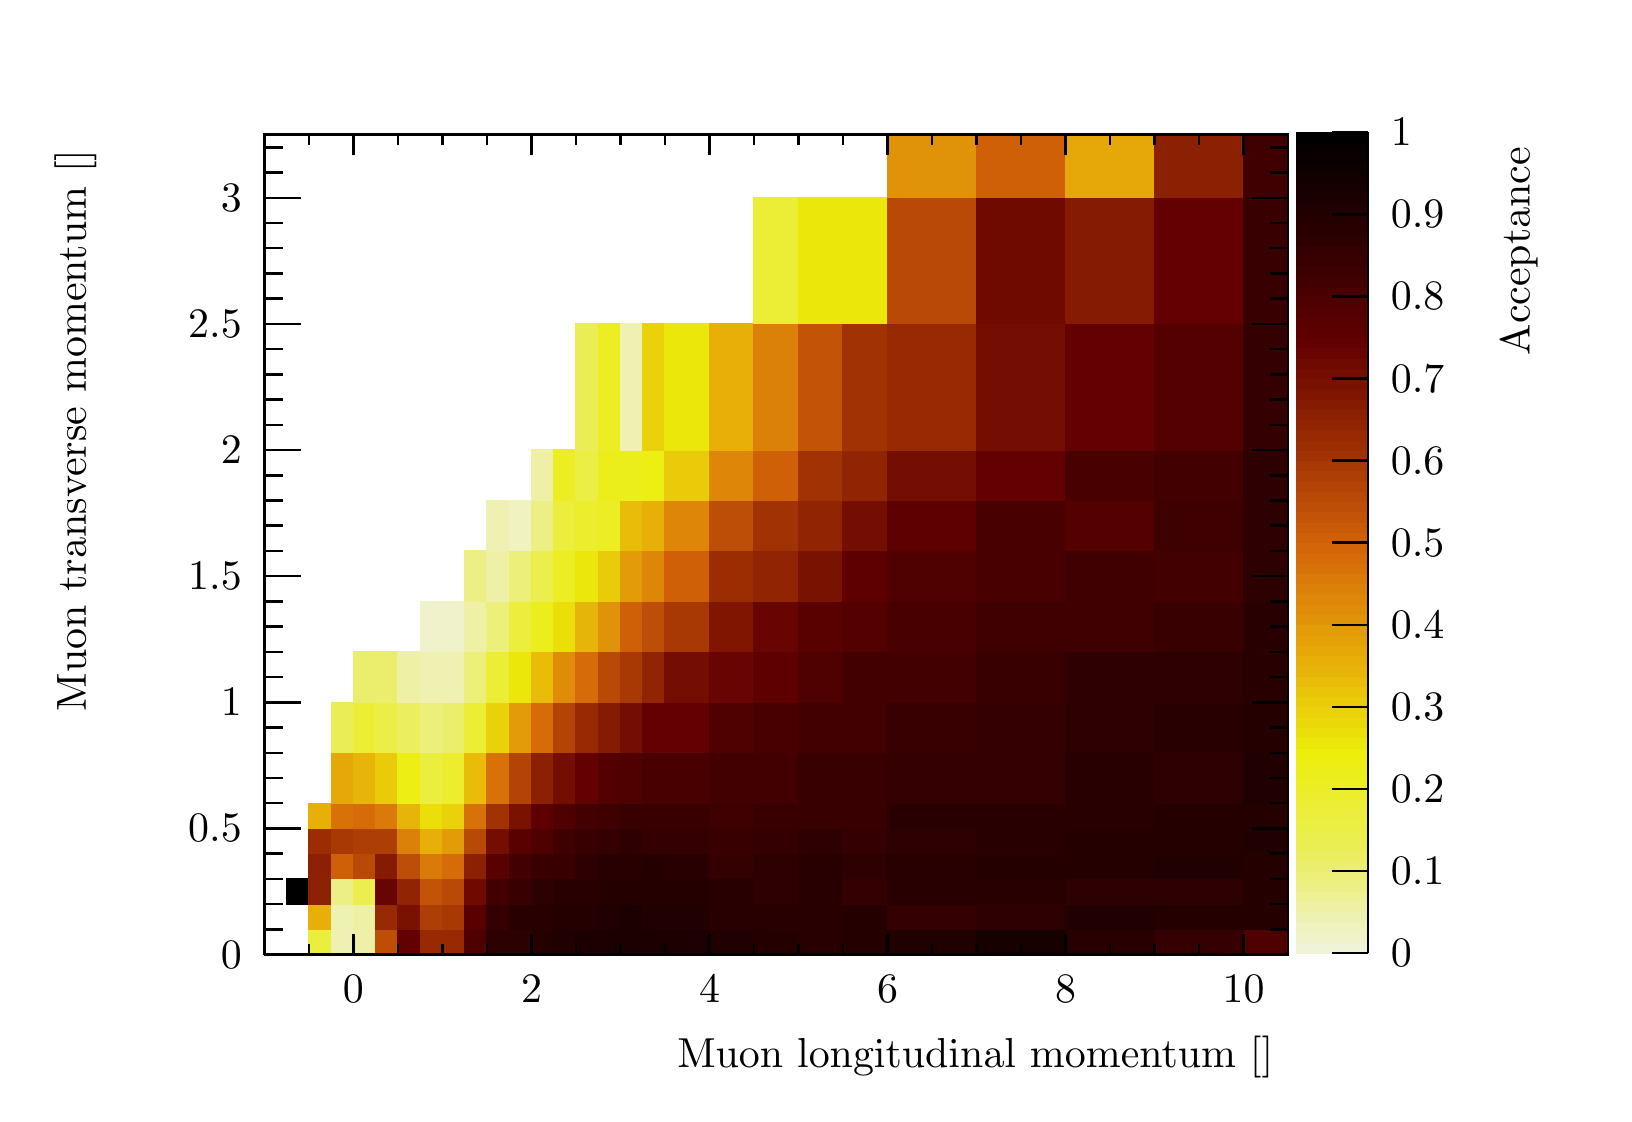
\begin{tikzpicture}
\pgfdeclareplotmark{cross} {
\pgfpathmoveto{\pgfpoint{-0.3\pgfplotmarksize}{\pgfplotmarksize}}
\pgfpathlineto{\pgfpoint{+0.3\pgfplotmarksize}{\pgfplotmarksize}}
\pgfpathlineto{\pgfpoint{+0.3\pgfplotmarksize}{0.3\pgfplotmarksize}}
\pgfpathlineto{\pgfpoint{+1\pgfplotmarksize}{0.3\pgfplotmarksize}}
\pgfpathlineto{\pgfpoint{+1\pgfplotmarksize}{-0.3\pgfplotmarksize}}
\pgfpathlineto{\pgfpoint{+0.3\pgfplotmarksize}{-0.3\pgfplotmarksize}}
\pgfpathlineto{\pgfpoint{+0.3\pgfplotmarksize}{-1.\pgfplotmarksize}}
\pgfpathlineto{\pgfpoint{-0.3\pgfplotmarksize}{-1.\pgfplotmarksize}}
\pgfpathlineto{\pgfpoint{-0.3\pgfplotmarksize}{-0.3\pgfplotmarksize}}
\pgfpathlineto{\pgfpoint{-1.\pgfplotmarksize}{-0.3\pgfplotmarksize}}
\pgfpathlineto{\pgfpoint{-1.\pgfplotmarksize}{0.3\pgfplotmarksize}}
\pgfpathlineto{\pgfpoint{-0.3\pgfplotmarksize}{0.3\pgfplotmarksize}}
\pgfpathclose
\pgfusepathqstroke
}
\pgfdeclareplotmark{cross*} {
\pgfpathmoveto{\pgfpoint{-0.3\pgfplotmarksize}{\pgfplotmarksize}}
\pgfpathlineto{\pgfpoint{+0.3\pgfplotmarksize}{\pgfplotmarksize}}
\pgfpathlineto{\pgfpoint{+0.3\pgfplotmarksize}{0.3\pgfplotmarksize}}
\pgfpathlineto{\pgfpoint{+1\pgfplotmarksize}{0.3\pgfplotmarksize}}
\pgfpathlineto{\pgfpoint{+1\pgfplotmarksize}{-0.3\pgfplotmarksize}}
\pgfpathlineto{\pgfpoint{+0.3\pgfplotmarksize}{-0.3\pgfplotmarksize}}
\pgfpathlineto{\pgfpoint{+0.3\pgfplotmarksize}{-1.\pgfplotmarksize}}
\pgfpathlineto{\pgfpoint{-0.3\pgfplotmarksize}{-1.\pgfplotmarksize}}
\pgfpathlineto{\pgfpoint{-0.3\pgfplotmarksize}{-0.3\pgfplotmarksize}}
\pgfpathlineto{\pgfpoint{-1.\pgfplotmarksize}{-0.3\pgfplotmarksize}}
\pgfpathlineto{\pgfpoint{-1.\pgfplotmarksize}{0.3\pgfplotmarksize}}
\pgfpathlineto{\pgfpoint{-0.3\pgfplotmarksize}{0.3\pgfplotmarksize}}
\pgfpathclose
\pgfusepathqfillstroke
}
\pgfdeclareplotmark{newstar} {
\pgfpathmoveto{\pgfqpoint{0pt}{\pgfplotmarksize}}
\pgfpathlineto{\pgfqpointpolar{44}{0.5\pgfplotmarksize}}
\pgfpathlineto{\pgfqpointpolar{18}{\pgfplotmarksize}}
\pgfpathlineto{\pgfqpointpolar{-20}{0.5\pgfplotmarksize}}
\pgfpathlineto{\pgfqpointpolar{-54}{\pgfplotmarksize}}
\pgfpathlineto{\pgfqpointpolar{-90}{0.5\pgfplotmarksize}}
\pgfpathlineto{\pgfqpointpolar{234}{\pgfplotmarksize}}
\pgfpathlineto{\pgfqpointpolar{198}{0.5\pgfplotmarksize}}
\pgfpathlineto{\pgfqpointpolar{162}{\pgfplotmarksize}}
\pgfpathlineto{\pgfqpointpolar{134}{0.5\pgfplotmarksize}}
\pgfpathclose
\pgfusepathqstroke
}
\pgfdeclareplotmark{newstar*} {
\pgfpathmoveto{\pgfqpoint{0pt}{\pgfplotmarksize}}
\pgfpathlineto{\pgfqpointpolar{44}{0.5\pgfplotmarksize}}
\pgfpathlineto{\pgfqpointpolar{18}{\pgfplotmarksize}}
\pgfpathlineto{\pgfqpointpolar{-20}{0.5\pgfplotmarksize}}
\pgfpathlineto{\pgfqpointpolar{-54}{\pgfplotmarksize}}
\pgfpathlineto{\pgfqpointpolar{-90}{0.5\pgfplotmarksize}}
\pgfpathlineto{\pgfqpointpolar{234}{\pgfplotmarksize}}
\pgfpathlineto{\pgfqpointpolar{198}{0.5\pgfplotmarksize}}
\pgfpathlineto{\pgfqpointpolar{162}{\pgfplotmarksize}}
\pgfpathlineto{\pgfqpointpolar{134}{0.5\pgfplotmarksize}}
\pgfpathclose
\pgfusepathqfillstroke
}
\definecolor{c}{rgb}{1,1,1};
\draw [color=c, fill=c] (0,0) rectangle (20,13.5227);
\draw [color=c, fill=c] (3,1.75795) rectangle (16,12.1705);
\definecolor{c}{rgb}{0,0,0};
\draw [c,line width=0.9] (3,1.75795) -- (3,12.1705) -- (16,12.1705) -- (16,1.75795) -- (3,1.75795);
\definecolor{c}{rgb}{1,1,1};
\draw [color=c, fill=c] (3,1.75795) rectangle (16,12.1705);
\definecolor{c}{rgb}{0,0,0};
\draw [c,line width=0.9] (3,1.75795) -- (3,12.1705) -- (16,12.1705) -- (16,1.75795) -- (3,1.75795);
\definecolor{c}{rgb}{0.922426,0.933333,0.238725};
\draw [color=c, fill=c] (3.56522,1.75795) rectangle (3.84783,2.07834);
\definecolor{c}{rgb}{0.936875,0.945351,0.697027};
\draw [color=c, fill=c] (3.84783,1.75795) rectangle (4.13043,2.07834);
\definecolor{c}{rgb}{0.933839,0.943453,0.645794};
\draw [color=c, fill=c] (4.13043,1.75795) rectangle (4.41304,2.07834);
\definecolor{c}{rgb}{0.742157,0.306863,0.0257353};
\draw [color=c, fill=c] (4.41304,1.75795) rectangle (4.69565,2.07834);
\definecolor{c}{rgb}{0.388235,0,0.00392157};
\draw [color=c, fill=c] (4.69565,1.75795) rectangle (4.97826,2.07834);
\definecolor{c}{rgb}{0.590809,0.159926,0.0110294};
\draw [color=c, fill=c] (4.97826,1.75795) rectangle (5.26087,2.07834);
\draw [color=c, fill=c] (5.26087,1.75795) rectangle (5.54348,2.07834);
\definecolor{c}{rgb}{0.308824,0,0.00392157};
\draw [color=c, fill=c] (5.54348,1.75795) rectangle (5.82609,2.07834);
\definecolor{c}{rgb}{0.176471,0,0.00392157};
\draw [color=c, fill=c] (5.82609,1.75795) rectangle (6.1087,2.07834);
\draw [color=c, fill=c] (6.1087,1.75795) rectangle (6.3913,2.07834);
\definecolor{c}{rgb}{0.143382,0,0.00318627};
\draw [color=c, fill=c] (6.3913,1.75795) rectangle (6.67391,2.07834);
\definecolor{c}{rgb}{0.126838,0,0.00281863};
\draw [color=c, fill=c] (6.67391,1.75795) rectangle (6.95652,2.07834);
\definecolor{c}{rgb}{0.110294,0,0.00245098};
\draw [color=c, fill=c] (6.95652,1.75795) rectangle (7.23913,2.07834);
\draw [color=c, fill=c] (7.23913,1.75795) rectangle (7.52174,2.07834);
\draw [color=c, fill=c] (7.52174,1.75795) rectangle (7.80435,2.07834);
\draw [color=c, fill=c] (7.80435,1.75795) rectangle (8.08696,2.07834);
\draw [color=c, fill=c] (8.08696,1.75795) rectangle (8.65217,2.07834);
\definecolor{c}{rgb}{0.126838,0,0.00281863};
\draw [color=c, fill=c] (8.65217,1.75795) rectangle (9.21739,2.07834);
\definecolor{c}{rgb}{0.143382,0,0.00318627};
\draw [color=c, fill=c] (9.21739,1.75795) rectangle (9.78261,2.07834);
\definecolor{c}{rgb}{0.159926,0,0.00355392};
\draw [color=c, fill=c] (9.78261,1.75795) rectangle (10.3478,2.07834);
\definecolor{c}{rgb}{0.143382,0,0.00318627};
\draw [color=c, fill=c] (10.3478,1.75795) rectangle (10.913,2.07834);
\definecolor{c}{rgb}{0.126838,0,0.00281863};
\draw [color=c, fill=c] (10.913,1.75795) rectangle (12.0435,2.07834);
\definecolor{c}{rgb}{0.0882353,0,0.00196078};
\draw [color=c, fill=c] (12.0435,1.75795) rectangle (13.1739,2.07834);
\definecolor{c}{rgb}{0.159926,0,0.00355392};
\draw [color=c, fill=c] (13.1739,1.75795) rectangle (14.3043,2.07834);
\definecolor{c}{rgb}{0.202941,0,0.00392157};
\draw [color=c, fill=c] (14.3043,1.75795) rectangle (15.4348,2.07834);
\definecolor{c}{rgb}{0.308824,0,0.00392157};
\draw [color=c, fill=c] (15.4348,1.75795) rectangle (16,2.07834);
\definecolor{c}{rgb}{0.904534,0.684559,0.0324755};
\draw [color=c, fill=c] (3.56522,2.07834) rectangle (3.84783,2.39872);
\definecolor{c}{rgb}{0.936875,0.945351,0.697027};
\draw [color=c, fill=c] (3.84783,2.07834) rectangle (4.13043,2.39872);
\definecolor{c}{rgb}{0.933839,0.943453,0.645794};
\draw [color=c, fill=c] (4.13043,2.07834) rectangle (4.41304,2.39872);
\definecolor{c}{rgb}{0.590809,0.159926,0.0110294};
\draw [color=c, fill=c] (4.41304,2.07834) rectangle (4.69565,2.39872);
\definecolor{c}{rgb}{0.479044,0.0716912,0.00710784};
\draw [color=c, fill=c] (4.69565,2.07834) rectangle (4.97826,2.39872);
\definecolor{c}{rgb}{0.680392,0.245098,0.0191176};
\draw [color=c, fill=c] (4.97826,2.07834) rectangle (5.26087,2.39872);
\definecolor{c}{rgb}{0.659804,0.22451,0.0169118};
\draw [color=c, fill=c] (5.26087,2.07834) rectangle (5.54348,2.39872);
\definecolor{c}{rgb}{0.348529,0,0.00392157};
\draw [color=c, fill=c] (5.54348,2.07834) rectangle (5.82609,2.39872);
\definecolor{c}{rgb}{0.202941,0,0.00392157};
\draw [color=c, fill=c] (5.82609,2.07834) rectangle (6.1087,2.39872);
\definecolor{c}{rgb}{0.159926,0,0.00355392};
\draw [color=c, fill=c] (6.1087,2.07834) rectangle (6.3913,2.39872);
\draw [color=c, fill=c] (6.3913,2.07834) rectangle (6.67391,2.39872);
\definecolor{c}{rgb}{0.143382,0,0.00318627};
\draw [color=c, fill=c] (6.67391,2.07834) rectangle (6.95652,2.39872);
\draw [color=c, fill=c] (6.95652,2.07834) rectangle (7.23913,2.39872);
\definecolor{c}{rgb}{0.126838,0,0.00281863};
\draw [color=c, fill=c] (7.23913,2.07834) rectangle (7.52174,2.39872);
\definecolor{c}{rgb}{0.110294,0,0.00245098};
\draw [color=c, fill=c] (7.52174,2.07834) rectangle (7.80435,2.39872);
\definecolor{c}{rgb}{0.126838,0,0.00281863};
\draw [color=c, fill=c] (7.80435,2.07834) rectangle (8.08696,2.39872);
\draw [color=c, fill=c] (8.08696,2.07834) rectangle (8.65217,2.39872);
\definecolor{c}{rgb}{0.159926,0,0.00355392};
\draw [color=c, fill=c] (8.65217,2.07834) rectangle (9.21739,2.39872);
\draw [color=c, fill=c] (9.21739,2.07834) rectangle (9.78261,2.39872);
\draw [color=c, fill=c] (9.78261,2.07834) rectangle (10.3478,2.39872);
\definecolor{c}{rgb}{0.143382,0,0.00318627};
\draw [color=c, fill=c] (10.3478,2.07834) rectangle (10.913,2.39872);
\definecolor{c}{rgb}{0.202941,0,0.00392157};
\draw [color=c, fill=c] (10.913,2.07834) rectangle (12.0435,2.39872);
\definecolor{c}{rgb}{0.176471,0,0.00392157};
\draw [color=c, fill=c] (12.0435,2.07834) rectangle (13.1739,2.39872);
\definecolor{c}{rgb}{0.126838,0,0.00281863};
\draw [color=c, fill=c] (13.1739,2.07834) rectangle (14.3043,2.39872);
\definecolor{c}{rgb}{0.143382,0,0.00318627};
\draw [color=c, fill=c] (14.3043,2.07834) rectangle (15.4348,2.39872);
\draw [color=c, fill=c] (15.4348,2.07834) rectangle (16,2.39872);
\definecolor{c}{rgb}{0.00551471,0,0.000122549};
\draw [color=c, fill=c] (3.28261,2.39872) rectangle (3.56522,2.71911);
\definecolor{c}{rgb}{0.548897,0.126838,0.00955882};
\draw [color=c, fill=c] (3.56522,2.39872) rectangle (3.84783,2.71911);
\definecolor{c}{rgb}{0.926755,0.939026,0.526249};
\draw [color=c, fill=c] (3.84783,2.39872) rectangle (4.13043,2.71911);
\definecolor{c}{rgb}{0.920221,0.933333,0.30049};
\draw [color=c, fill=c] (4.13043,2.39872) rectangle (4.41304,2.71911);
\definecolor{c}{rgb}{0.409191,0.0165441,0.00465686};
\draw [color=c, fill=c] (4.41304,2.39872) rectangle (4.69565,2.71911);
\definecolor{c}{rgb}{0.569853,0.143382,0.0102941};
\draw [color=c, fill=c] (4.69565,2.39872) rectangle (4.97826,2.71911);
\definecolor{c}{rgb}{0.762745,0.327451,0.0279412};
\draw [color=c, fill=c] (4.97826,2.39872) rectangle (5.26087,2.71911);
\definecolor{c}{rgb}{0.721569,0.286275,0.0235294};
\draw [color=c, fill=c] (5.26087,2.39872) rectangle (5.54348,2.71911);
\definecolor{c}{rgb}{0.437132,0.0386029,0.00563726};
\draw [color=c, fill=c] (5.54348,2.39872) rectangle (5.82609,2.71911);
\definecolor{c}{rgb}{0.2625,0,0.00392157};
\draw [color=c, fill=c] (5.82609,2.39872) rectangle (6.1087,2.71911);
\definecolor{c}{rgb}{0.222794,0,0.00392157};
\draw [color=c, fill=c] (6.1087,2.39872) rectangle (6.3913,2.71911);
\definecolor{c}{rgb}{0.176471,0,0.00392157};
\draw [color=c, fill=c] (6.3913,2.39872) rectangle (6.67391,2.71911);
\definecolor{c}{rgb}{0.159926,0,0.00355392};
\draw [color=c, fill=c] (6.67391,2.39872) rectangle (6.95652,2.71911);
\draw [color=c, fill=c] (6.95652,2.39872) rectangle (7.23913,2.71911);
\definecolor{c}{rgb}{0.143382,0,0.00318627};
\draw [color=c, fill=c] (7.23913,2.39872) rectangle (7.52174,2.71911);
\draw [color=c, fill=c] (7.52174,2.39872) rectangle (7.80435,2.71911);
\draw [color=c, fill=c] (7.80435,2.39872) rectangle (8.08696,2.71911);
\draw [color=c, fill=c] (8.08696,2.39872) rectangle (8.65217,2.71911);
\definecolor{c}{rgb}{0.159926,0,0.00355392};
\draw [color=c, fill=c] (8.65217,2.39872) rectangle (9.21739,2.71911);
\definecolor{c}{rgb}{0.176471,0,0.00392157};
\draw [color=c, fill=c] (9.21739,2.39872) rectangle (9.78261,2.71911);
\definecolor{c}{rgb}{0.159926,0,0.00355392};
\draw [color=c, fill=c] (9.78261,2.39872) rectangle (10.3478,2.71911);
\definecolor{c}{rgb}{0.202941,0,0.00392157};
\draw [color=c, fill=c] (10.3478,2.39872) rectangle (10.913,2.71911);
\definecolor{c}{rgb}{0.159926,0,0.00355392};
\draw [color=c, fill=c] (10.913,2.39872) rectangle (12.0435,2.71911);
\draw [color=c, fill=c] (12.0435,2.39872) rectangle (13.1739,2.71911);
\definecolor{c}{rgb}{0.176471,0,0.00392157};
\draw [color=c, fill=c] (13.1739,2.39872) rectangle (14.3043,2.71911);
\draw [color=c, fill=c] (14.3043,2.39872) rectangle (15.4348,2.71911);
\definecolor{c}{rgb}{0.143382,0,0.00318627};
\draw [color=c, fill=c] (15.4348,2.39872) rectangle (16,2.71911);
\definecolor{c}{rgb}{0.548897,0.126838,0.00955882};
\draw [color=c, fill=c] (3.56522,2.71911) rectangle (3.84783,3.03949);
\definecolor{c}{rgb}{0.810784,0.37549,0.0330882};
\draw [color=c, fill=c] (3.84783,2.71911) rectangle (4.13043,3.03949);
\definecolor{c}{rgb}{0.721569,0.286275,0.0235294};
\draw [color=c, fill=c] (4.13043,2.71911) rectangle (4.41304,3.03949);
\definecolor{c}{rgb}{0.520956,0.104779,0.00857843};
\draw [color=c, fill=c] (4.41304,2.71911) rectangle (4.69565,3.03949);
\definecolor{c}{rgb}{0.742157,0.306863,0.0257353};
\draw [color=c, fill=c] (4.69565,2.71911) rectangle (4.97826,3.03949);
\definecolor{c}{rgb}{0.853431,0.478186,0.0340686};
\draw [color=c, fill=c] (4.97826,2.71911) rectangle (5.26087,3.03949);
\definecolor{c}{rgb}{0.83799,0.420711,0.0349265};
\draw [color=c, fill=c] (5.26087,2.71911) rectangle (5.54348,3.03949);
\definecolor{c}{rgb}{0.548897,0.126838,0.00955882};
\draw [color=c, fill=c] (5.54348,2.71911) rectangle (5.82609,3.03949);
\definecolor{c}{rgb}{0.348529,0,0.00392157};
\draw [color=c, fill=c] (5.82609,2.71911) rectangle (6.1087,3.03949);
\definecolor{c}{rgb}{0.2625,0,0.00392157};
\draw [color=c, fill=c] (6.1087,2.71911) rectangle (6.3913,3.03949);
\definecolor{c}{rgb}{0.222794,0,0.00392157};
\draw [color=c, fill=c] (6.3913,2.71911) rectangle (6.67391,3.03949);
\draw [color=c, fill=c] (6.67391,2.71911) rectangle (6.95652,3.03949);
\definecolor{c}{rgb}{0.176471,0,0.00392157};
\draw [color=c, fill=c] (6.95652,2.71911) rectangle (7.23913,3.03949);
\definecolor{c}{rgb}{0.159926,0,0.00355392};
\draw [color=c, fill=c] (7.23913,2.71911) rectangle (7.52174,3.03949);
\draw [color=c, fill=c] (7.52174,2.71911) rectangle (7.80435,3.03949);
\definecolor{c}{rgb}{0.143382,0,0.00318627};
\draw [color=c, fill=c] (7.80435,2.71911) rectangle (8.08696,3.03949);
\definecolor{c}{rgb}{0.159926,0,0.00355392};
\draw [color=c, fill=c] (8.08696,2.71911) rectangle (8.65217,3.03949);
\definecolor{c}{rgb}{0.202941,0,0.00392157};
\draw [color=c, fill=c] (8.65217,2.71911) rectangle (9.21739,3.03949);
\definecolor{c}{rgb}{0.176471,0,0.00392157};
\draw [color=c, fill=c] (9.21739,2.71911) rectangle (9.78261,3.03949);
\definecolor{c}{rgb}{0.159926,0,0.00355392};
\draw [color=c, fill=c] (9.78261,2.71911) rectangle (10.3478,3.03949);
\definecolor{c}{rgb}{0.176471,0,0.00392157};
\draw [color=c, fill=c] (10.3478,2.71911) rectangle (10.913,3.03949);
\definecolor{c}{rgb}{0.159926,0,0.00355392};
\draw [color=c, fill=c] (10.913,2.71911) rectangle (12.0435,3.03949);
\definecolor{c}{rgb}{0.143382,0,0.00318627};
\draw [color=c, fill=c] (12.0435,2.71911) rectangle (13.1739,3.03949);
\draw [color=c, fill=c] (13.1739,2.71911) rectangle (14.3043,3.03949);
\definecolor{c}{rgb}{0.126838,0,0.00281863};
\draw [color=c, fill=c] (14.3043,2.71911) rectangle (15.4348,3.03949);
\definecolor{c}{rgb}{0.143382,0,0.00318627};
\draw [color=c, fill=c] (15.4348,2.71911) rectangle (16,3.03949);
\definecolor{c}{rgb}{0.611765,0.176471,0.0117647};
\draw [color=c, fill=c] (3.56522,3.03949) rectangle (3.84783,3.35988);
\definecolor{c}{rgb}{0.659804,0.22451,0.0169118};
\draw [color=c, fill=c] (3.84783,3.03949) rectangle (4.13043,3.35988);
\definecolor{c}{rgb}{0.680392,0.245098,0.0191176};
\draw [color=c, fill=c] (4.13043,3.03949) rectangle (4.41304,3.35988);
\draw [color=c, fill=c] (4.41304,3.03949) rectangle (4.69565,3.35988);
\definecolor{c}{rgb}{0.860049,0.502819,0.033701};
\draw [color=c, fill=c] (4.69565,3.03949) rectangle (4.97826,3.35988);
\definecolor{c}{rgb}{0.904534,0.684559,0.0324755};
\draw [color=c, fill=c] (4.97826,3.03949) rectangle (5.26087,3.35988);
\definecolor{c}{rgb}{0.888726,0.609559,0.0321078};
\draw [color=c, fill=c] (5.26087,3.03949) rectangle (5.54348,3.35988);
\definecolor{c}{rgb}{0.721569,0.286275,0.0235294};
\draw [color=c, fill=c] (5.54348,3.03949) rectangle (5.82609,3.35988);
\definecolor{c}{rgb}{0.458088,0.0551471,0.00637255};
\draw [color=c, fill=c] (5.82609,3.03949) rectangle (6.1087,3.35988);
\definecolor{c}{rgb}{0.348529,0,0.00392157};
\draw [color=c, fill=c] (6.1087,3.03949) rectangle (6.3913,3.35988);
\definecolor{c}{rgb}{0.308824,0,0.00392157};
\draw [color=c, fill=c] (6.3913,3.03949) rectangle (6.67391,3.35988);
\definecolor{c}{rgb}{0.242647,0,0.00392157};
\draw [color=c, fill=c] (6.67391,3.03949) rectangle (6.95652,3.35988);
\definecolor{c}{rgb}{0.222794,0,0.00392157};
\draw [color=c, fill=c] (6.95652,3.03949) rectangle (7.23913,3.35988);
\definecolor{c}{rgb}{0.202941,0,0.00392157};
\draw [color=c, fill=c] (7.23913,3.03949) rectangle (7.52174,3.35988);
\definecolor{c}{rgb}{0.176471,0,0.00392157};
\draw [color=c, fill=c] (7.52174,3.03949) rectangle (7.80435,3.35988);
\definecolor{c}{rgb}{0.202941,0,0.00392157};
\draw [color=c, fill=c] (7.80435,3.03949) rectangle (8.08696,3.35988);
\draw [color=c, fill=c] (8.08696,3.03949) rectangle (8.65217,3.35988);
\definecolor{c}{rgb}{0.222794,0,0.00392157};
\draw [color=c, fill=c] (8.65217,3.03949) rectangle (9.21739,3.35988);
\definecolor{c}{rgb}{0.202941,0,0.00392157};
\draw [color=c, fill=c] (9.21739,3.03949) rectangle (9.78261,3.35988);
\definecolor{c}{rgb}{0.176471,0,0.00392157};
\draw [color=c, fill=c] (9.78261,3.03949) rectangle (10.3478,3.35988);
\definecolor{c}{rgb}{0.202941,0,0.00392157};
\draw [color=c, fill=c] (10.3478,3.03949) rectangle (10.913,3.35988);
\definecolor{c}{rgb}{0.176471,0,0.00392157};
\draw [color=c, fill=c] (10.913,3.03949) rectangle (12.0435,3.35988);
\definecolor{c}{rgb}{0.159926,0,0.00355392};
\draw [color=c, fill=c] (12.0435,3.03949) rectangle (13.1739,3.35988);
\definecolor{c}{rgb}{0.143382,0,0.00318627};
\draw [color=c, fill=c] (13.1739,3.03949) rectangle (14.3043,3.35988);
\draw [color=c, fill=c] (14.3043,3.03949) rectangle (15.4348,3.35988);
\definecolor{c}{rgb}{0.126838,0,0.00281863};
\draw [color=c, fill=c] (15.4348,3.03949) rectangle (16,3.35988);
\definecolor{c}{rgb}{0.904534,0.684559,0.0324755};
\draw [color=c, fill=c] (3.56522,3.35988) rectangle (3.84783,3.68026);
\definecolor{c}{rgb}{0.844608,0.445343,0.0345588};
\draw [color=c, fill=c] (3.84783,3.35988) rectangle (4.13043,3.68026);
\definecolor{c}{rgb}{0.83799,0.420711,0.0349265};
\draw [color=c, fill=c] (4.13043,3.35988) rectangle (4.41304,3.68026);
\definecolor{c}{rgb}{0.853431,0.478186,0.0340686};
\draw [color=c, fill=c] (4.41304,3.35988) rectangle (4.69565,3.68026);
\definecolor{c}{rgb}{0.907108,0.710294,0.0335784};
\draw [color=c, fill=c] (4.69565,3.35988) rectangle (4.97826,3.68026);
\definecolor{c}{rgb}{0.923407,0.873284,0.0405637};
\draw [color=c, fill=c] (4.97826,3.35988) rectangle (5.26087,3.68026);
\definecolor{c}{rgb}{0.91826,0.821814,0.0383578};
\draw [color=c, fill=c] (5.26087,3.35988) rectangle (5.54348,3.68026);
\definecolor{c}{rgb}{0.844608,0.445343,0.0345588};
\draw [color=c, fill=c] (5.54348,3.35988) rectangle (5.82609,3.68026);
\definecolor{c}{rgb}{0.632353,0.197059,0.0139706};
\draw [color=c, fill=c] (5.82609,3.35988) rectangle (6.1087,3.68026);
\definecolor{c}{rgb}{0.479044,0.0716912,0.00710784};
\draw [color=c, fill=c] (6.1087,3.35988) rectangle (6.3913,3.68026);
\definecolor{c}{rgb}{0.368382,0,0.00392157};
\draw [color=c, fill=c] (6.3913,3.35988) rectangle (6.67391,3.68026);
\definecolor{c}{rgb}{0.308824,0,0.00392157};
\draw [color=c, fill=c] (6.67391,3.35988) rectangle (6.95652,3.68026);
\definecolor{c}{rgb}{0.2625,0,0.00392157};
\draw [color=c, fill=c] (6.95652,3.35988) rectangle (7.23913,3.68026);
\definecolor{c}{rgb}{0.242647,0,0.00392157};
\draw [color=c, fill=c] (7.23913,3.35988) rectangle (7.52174,3.68026);
\definecolor{c}{rgb}{0.222794,0,0.00392157};
\draw [color=c, fill=c] (7.52174,3.35988) rectangle (7.80435,3.68026);
\draw [color=c, fill=c] (7.80435,3.35988) rectangle (8.08696,3.68026);
\draw [color=c, fill=c] (8.08696,3.35988) rectangle (8.65217,3.68026);
\definecolor{c}{rgb}{0.242647,0,0.00392157};
\draw [color=c, fill=c] (8.65217,3.35988) rectangle (9.21739,3.68026);
\definecolor{c}{rgb}{0.222794,0,0.00392157};
\draw [color=c, fill=c] (9.21739,3.35988) rectangle (9.78261,3.68026);
\draw [color=c, fill=c] (9.78261,3.35988) rectangle (10.3478,3.68026);
\draw [color=c, fill=c] (10.3478,3.35988) rectangle (10.913,3.68026);
\definecolor{c}{rgb}{0.159926,0,0.00355392};
\draw [color=c, fill=c] (10.913,3.35988) rectangle (12.0435,3.68026);
\draw [color=c, fill=c] (12.0435,3.35988) rectangle (13.1739,3.68026);
\draw [color=c, fill=c] (13.1739,3.35988) rectangle (14.3043,3.68026);
\definecolor{c}{rgb}{0.143382,0,0.00318627};
\draw [color=c, fill=c] (14.3043,3.35988) rectangle (15.4348,3.68026);
\draw [color=c, fill=c] (15.4348,3.35988) rectangle (16,3.68026);
\definecolor{c}{rgb}{0.901961,0.658824,0.0313726};
\draw [color=c, fill=c] (3.84783,3.68026) rectangle (4.13043,4.32103);
\definecolor{c}{rgb}{0.907108,0.710294,0.0335784};
\draw [color=c, fill=c] (4.13043,3.68026) rectangle (4.41304,4.32103);
\definecolor{c}{rgb}{0.915686,0.796078,0.0372549};
\draw [color=c, fill=c] (4.41304,3.68026) rectangle (4.69565,4.32103);
\definecolor{c}{rgb}{0.928309,0.933333,0.0740196};
\draw [color=c, fill=c] (4.69565,3.68026) rectangle (4.97826,4.32103);
\definecolor{c}{rgb}{0.922426,0.933333,0.238725};
\draw [color=c, fill=c] (4.97826,3.68026) rectangle (5.26087,4.32103);
\definecolor{c}{rgb}{0.924632,0.933333,0.176961};
\draw [color=c, fill=c] (5.26087,3.68026) rectangle (5.54348,4.32103);
\definecolor{c}{rgb}{0.909681,0.736029,0.0346814};
\draw [color=c, fill=c] (5.54348,3.68026) rectangle (5.82609,4.32103);
\definecolor{c}{rgb}{0.844608,0.445343,0.0345588};
\draw [color=c, fill=c] (5.82609,3.68026) rectangle (6.1087,4.32103);
\definecolor{c}{rgb}{0.70098,0.265686,0.0213235};
\draw [color=c, fill=c] (6.1087,3.68026) rectangle (6.3913,4.32103);
\definecolor{c}{rgb}{0.548897,0.126838,0.00955882};
\draw [color=c, fill=c] (6.3913,3.68026) rectangle (6.67391,4.32103);
\definecolor{c}{rgb}{0.458088,0.0551471,0.00637255};
\draw [color=c, fill=c] (6.67391,3.68026) rectangle (6.95652,4.32103);
\definecolor{c}{rgb}{0.388235,0,0.00392157};
\draw [color=c, fill=c] (6.95652,3.68026) rectangle (7.23913,4.32103);
\definecolor{c}{rgb}{0.328676,0,0.00392157};
\draw [color=c, fill=c] (7.23913,3.68026) rectangle (7.52174,4.32103);
\definecolor{c}{rgb}{0.308824,0,0.00392157};
\draw [color=c, fill=c] (7.52174,3.68026) rectangle (7.80435,4.32103);
\definecolor{c}{rgb}{0.282353,0,0.00392157};
\draw [color=c, fill=c] (7.80435,3.68026) rectangle (8.08696,4.32103);
\draw [color=c, fill=c] (8.08696,3.68026) rectangle (8.65217,4.32103);
\definecolor{c}{rgb}{0.2625,0,0.00392157};
\draw [color=c, fill=c] (8.65217,3.68026) rectangle (9.21739,4.32103);
\draw [color=c, fill=c] (9.21739,3.68026) rectangle (9.78261,4.32103);
\definecolor{c}{rgb}{0.222794,0,0.00392157};
\draw [color=c, fill=c] (9.78261,3.68026) rectangle (10.3478,4.32103);
\draw [color=c, fill=c] (10.3478,3.68026) rectangle (10.913,4.32103);
\definecolor{c}{rgb}{0.202941,0,0.00392157};
\draw [color=c, fill=c] (10.913,3.68026) rectangle (12.0435,4.32103);
\draw [color=c, fill=c] (12.0435,3.68026) rectangle (13.1739,4.32103);
\definecolor{c}{rgb}{0.159926,0,0.00355392};
\draw [color=c, fill=c] (13.1739,3.68026) rectangle (14.3043,4.32103);
\definecolor{c}{rgb}{0.176471,0,0.00392157};
\draw [color=c, fill=c] (14.3043,3.68026) rectangle (15.4348,4.32103);
\definecolor{c}{rgb}{0.126838,0,0.00281863};
\draw [color=c, fill=c] (15.4348,3.68026) rectangle (16,4.32103);
\definecolor{c}{rgb}{0.919118,0.933333,0.331373};
\draw [color=c, fill=c] (3.84783,4.32103) rectangle (4.13043,4.9618);
\definecolor{c}{rgb}{0.923529,0.933333,0.207843};
\draw [color=c, fill=c] (4.13043,4.32103) rectangle (4.41304,4.9618);
\definecolor{c}{rgb}{0.921324,0.933333,0.269608};
\draw [color=c, fill=c] (4.41304,4.32103) rectangle (4.69565,4.9618);
\definecolor{c}{rgb}{0.917647,0.933333,0.372549};
\draw [color=c, fill=c] (4.69565,4.32103) rectangle (4.97826,4.9618);
\definecolor{c}{rgb}{0.923719,0.937128,0.475016};
\draw [color=c, fill=c] (4.97826,4.32103) rectangle (5.26087,4.9618);
\definecolor{c}{rgb}{0.920683,0.935231,0.423782};
\draw [color=c, fill=c] (5.26087,4.32103) rectangle (5.54348,4.9618);
\definecolor{c}{rgb}{0.923529,0.933333,0.207843};
\draw [color=c, fill=c] (5.54348,4.32103) rectangle (5.82609,4.9618);
\definecolor{c}{rgb}{0.91826,0.821814,0.0383578};
\draw [color=c, fill=c] (5.82609,4.32103) rectangle (6.1087,4.9618);
\definecolor{c}{rgb}{0.888726,0.609559,0.0321078};
\draw [color=c, fill=c] (6.1087,4.32103) rectangle (6.3913,4.9618);
\definecolor{c}{rgb}{0.83799,0.420711,0.0349265};
\draw [color=c, fill=c] (6.3913,4.32103) rectangle (6.67391,4.9618);
\definecolor{c}{rgb}{0.70098,0.265686,0.0213235};
\draw [color=c, fill=c] (6.67391,4.32103) rectangle (6.95652,4.9618);
\definecolor{c}{rgb}{0.590809,0.159926,0.0110294};
\draw [color=c, fill=c] (6.95652,4.32103) rectangle (7.23913,4.9618);
\definecolor{c}{rgb}{0.520956,0.104779,0.00857843};
\draw [color=c, fill=c] (7.23913,4.32103) rectangle (7.52174,4.9618);
\definecolor{c}{rgb}{0.458088,0.0551471,0.00637255};
\draw [color=c, fill=c] (7.52174,4.32103) rectangle (7.80435,4.9618);
\definecolor{c}{rgb}{0.388235,0,0.00392157};
\draw [color=c, fill=c] (7.80435,4.32103) rectangle (8.08696,4.9618);
\draw [color=c, fill=c] (8.08696,4.32103) rectangle (8.65217,4.9618);
\definecolor{c}{rgb}{0.308824,0,0.00392157};
\draw [color=c, fill=c] (8.65217,4.32103) rectangle (9.21739,4.9618);
\definecolor{c}{rgb}{0.282353,0,0.00392157};
\draw [color=c, fill=c] (9.21739,4.32103) rectangle (9.78261,4.9618);
\definecolor{c}{rgb}{0.2625,0,0.00392157};
\draw [color=c, fill=c] (9.78261,4.32103) rectangle (10.3478,4.9618);
\draw [color=c, fill=c] (10.3478,4.32103) rectangle (10.913,4.9618);
\definecolor{c}{rgb}{0.222794,0,0.00392157};
\draw [color=c, fill=c] (10.913,4.32103) rectangle (12.0435,4.9618);
\definecolor{c}{rgb}{0.202941,0,0.00392157};
\draw [color=c, fill=c] (12.0435,4.32103) rectangle (13.1739,4.9618);
\definecolor{c}{rgb}{0.176471,0,0.00392157};
\draw [color=c, fill=c] (13.1739,4.32103) rectangle (14.3043,4.9618);
\definecolor{c}{rgb}{0.159926,0,0.00355392};
\draw [color=c, fill=c] (14.3043,4.32103) rectangle (15.4348,4.9618);
\definecolor{c}{rgb}{0.143382,0,0.00318627};
\draw [color=c, fill=c] (15.4348,4.32103) rectangle (16,4.9618);
\definecolor{c}{rgb}{0.920683,0.935231,0.423782};
\draw [color=c, fill=c] (4.13043,4.9618) rectangle (4.41304,5.60257);
\draw [color=c, fill=c] (4.41304,4.9618) rectangle (4.69565,5.60257);
\definecolor{c}{rgb}{0.933839,0.943453,0.645794};
\draw [color=c, fill=c] (4.69565,4.9618) rectangle (4.97826,5.60257);
\definecolor{c}{rgb}{0.936875,0.945351,0.697027};
\draw [color=c, fill=c] (4.97826,4.9618) rectangle (5.26087,5.60257);
\draw [color=c, fill=c] (5.26087,4.9618) rectangle (5.54348,5.60257);
\definecolor{c}{rgb}{0.923719,0.937128,0.475016};
\draw [color=c, fill=c] (5.54348,4.9618) rectangle (5.82609,5.60257);
\definecolor{c}{rgb}{0.923529,0.933333,0.207843};
\draw [color=c, fill=c] (5.82609,4.9618) rectangle (6.1087,5.60257);
\definecolor{c}{rgb}{0.926838,0.907598,0.0420343};
\draw [color=c, fill=c] (6.1087,4.9618) rectangle (6.3913,5.60257);
\definecolor{c}{rgb}{0.909681,0.736029,0.0346814};
\draw [color=c, fill=c] (6.3913,4.9618) rectangle (6.67391,5.60257);
\definecolor{c}{rgb}{0.873284,0.552083,0.0329657};
\draw [color=c, fill=c] (6.67391,4.9618) rectangle (6.95652,5.60257);
\definecolor{c}{rgb}{0.83799,0.420711,0.0349265};
\draw [color=c, fill=c] (6.95652,4.9618) rectangle (7.23913,5.60257);
\definecolor{c}{rgb}{0.721569,0.286275,0.0235294};
\draw [color=c, fill=c] (7.23913,4.9618) rectangle (7.52174,5.60257);
\definecolor{c}{rgb}{0.659804,0.22451,0.0169118};
\draw [color=c, fill=c] (7.52174,4.9618) rectangle (7.80435,5.60257);
\definecolor{c}{rgb}{0.569853,0.143382,0.0102941};
\draw [color=c, fill=c] (7.80435,4.9618) rectangle (8.08696,5.60257);
\definecolor{c}{rgb}{0.458088,0.0551471,0.00637255};
\draw [color=c, fill=c] (8.08696,4.9618) rectangle (8.65217,5.60257);
\definecolor{c}{rgb}{0.409191,0.0165441,0.00465686};
\draw [color=c, fill=c] (8.65217,4.9618) rectangle (9.21739,5.60257);
\definecolor{c}{rgb}{0.368382,0,0.00392157};
\draw [color=c, fill=c] (9.21739,4.9618) rectangle (9.78261,5.60257);
\definecolor{c}{rgb}{0.308824,0,0.00392157};
\draw [color=c, fill=c] (9.78261,4.9618) rectangle (10.3478,5.60257);
\definecolor{c}{rgb}{0.2625,0,0.00392157};
\draw [color=c, fill=c] (10.3478,4.9618) rectangle (10.913,5.60257);
\draw [color=c, fill=c] (10.913,4.9618) rectangle (12.0435,5.60257);
\definecolor{c}{rgb}{0.222794,0,0.00392157};
\draw [color=c, fill=c] (12.0435,4.9618) rectangle (13.1739,5.60257);
\definecolor{c}{rgb}{0.176471,0,0.00392157};
\draw [color=c, fill=c] (13.1739,4.9618) rectangle (14.3043,5.60257);
\draw [color=c, fill=c] (14.3043,4.9618) rectangle (15.4348,5.60257);
\definecolor{c}{rgb}{0.159926,0,0.00355392};
\draw [color=c, fill=c] (15.4348,4.9618) rectangle (16,5.60257);
\definecolor{c}{rgb}{0.942948,0.949146,0.799494};
\draw [color=c, fill=c] (4.97826,5.60257) rectangle (5.26087,6.24334);
\draw [color=c, fill=c] (5.26087,5.60257) rectangle (5.54348,6.24334);
\definecolor{c}{rgb}{0.933839,0.943453,0.645794};
\draw [color=c, fill=c] (5.54348,5.60257) rectangle (5.82609,6.24334);
\definecolor{c}{rgb}{0.923719,0.937128,0.475016};
\draw [color=c, fill=c] (5.82609,5.60257) rectangle (6.1087,6.24334);
\definecolor{c}{rgb}{0.922426,0.933333,0.238725};
\draw [color=c, fill=c] (6.1087,5.60257) rectangle (6.3913,6.24334);
\definecolor{c}{rgb}{0.927206,0.933333,0.104902};
\draw [color=c, fill=c] (6.3913,5.60257) rectangle (6.67391,6.24334);
\definecolor{c}{rgb}{0.923407,0.873284,0.0405637};
\draw [color=c, fill=c] (6.67391,5.60257) rectangle (6.95652,6.24334);
\definecolor{c}{rgb}{0.907108,0.710294,0.0335784};
\draw [color=c, fill=c] (6.95652,5.60257) rectangle (7.23913,6.24334);
\definecolor{c}{rgb}{0.879902,0.576716,0.032598};
\draw [color=c, fill=c] (7.23913,5.60257) rectangle (7.52174,6.24334);
\definecolor{c}{rgb}{0.810784,0.37549,0.0330882};
\draw [color=c, fill=c] (7.52174,5.60257) rectangle (7.80435,6.24334);
\definecolor{c}{rgb}{0.742157,0.306863,0.0257353};
\draw [color=c, fill=c] (7.80435,5.60257) rectangle (8.08696,6.24334);
\definecolor{c}{rgb}{0.659804,0.22451,0.0169118};
\draw [color=c, fill=c] (8.08696,5.60257) rectangle (8.65217,6.24334);
\definecolor{c}{rgb}{0.5,0.0882353,0.00784314};
\draw [color=c, fill=c] (8.65217,5.60257) rectangle (9.21739,6.24334);
\definecolor{c}{rgb}{0.409191,0.0165441,0.00465686};
\draw [color=c, fill=c] (9.21739,5.60257) rectangle (9.78261,6.24334);
\definecolor{c}{rgb}{0.348529,0,0.00392157};
\draw [color=c, fill=c] (9.78261,5.60257) rectangle (10.3478,6.24334);
\definecolor{c}{rgb}{0.328676,0,0.00392157};
\draw [color=c, fill=c] (10.3478,5.60257) rectangle (10.913,6.24334);
\definecolor{c}{rgb}{0.282353,0,0.00392157};
\draw [color=c, fill=c] (10.913,5.60257) rectangle (12.0435,6.24334);
\definecolor{c}{rgb}{0.242647,0,0.00392157};
\draw [color=c, fill=c] (12.0435,5.60257) rectangle (13.1739,6.24334);
\draw [color=c, fill=c] (13.1739,5.60257) rectangle (14.3043,6.24334);
\definecolor{c}{rgb}{0.222794,0,0.00392157};
\draw [color=c, fill=c] (14.3043,5.60257) rectangle (15.4348,6.24334);
\definecolor{c}{rgb}{0.159926,0,0.00355392};
\draw [color=c, fill=c] (15.4348,5.60257) rectangle (16,6.24334);
\definecolor{c}{rgb}{0.926755,0.939026,0.526249};
\draw [color=c, fill=c] (5.54348,6.24334) rectangle (5.82609,6.88411);
\definecolor{c}{rgb}{0.933839,0.943453,0.645794};
\draw [color=c, fill=c] (5.82609,6.24334) rectangle (6.1087,6.88411);
\definecolor{c}{rgb}{0.923719,0.937128,0.475016};
\draw [color=c, fill=c] (6.1087,6.24334) rectangle (6.3913,6.88411);
\definecolor{c}{rgb}{0.920221,0.933333,0.30049};
\draw [color=c, fill=c] (6.3913,6.24334) rectangle (6.67391,6.88411);
\definecolor{c}{rgb}{0.926103,0.933333,0.135784};
\draw [color=c, fill=c] (6.67391,6.24334) rectangle (6.95652,6.88411);
\definecolor{c}{rgb}{0.926838,0.907598,0.0420343};
\draw [color=c, fill=c] (6.95652,6.24334) rectangle (7.23913,6.88411);
\definecolor{c}{rgb}{0.915686,0.796078,0.0372549};
\draw [color=c, fill=c] (7.23913,6.24334) rectangle (7.52174,6.88411);
\definecolor{c}{rgb}{0.888726,0.609559,0.0321078};
\draw [color=c, fill=c] (7.52174,6.24334) rectangle (7.80435,6.88411);
\definecolor{c}{rgb}{0.866667,0.527451,0.0333333};
\draw [color=c, fill=c] (7.80435,6.24334) rectangle (8.08696,6.88411);
\definecolor{c}{rgb}{0.810784,0.37549,0.0330882};
\draw [color=c, fill=c] (8.08696,6.24334) rectangle (8.65217,6.88411);
\definecolor{c}{rgb}{0.611765,0.176471,0.0117647};
\draw [color=c, fill=c] (8.65217,6.24334) rectangle (9.21739,6.88411);
\definecolor{c}{rgb}{0.569853,0.143382,0.0102941};
\draw [color=c, fill=c] (9.21739,6.24334) rectangle (9.78261,6.88411);
\definecolor{c}{rgb}{0.479044,0.0716912,0.00710784};
\draw [color=c, fill=c] (9.78261,6.24334) rectangle (10.3478,6.88411);
\definecolor{c}{rgb}{0.368382,0,0.00392157};
\draw [color=c, fill=c] (10.3478,6.24334) rectangle (10.913,6.88411);
\definecolor{c}{rgb}{0.308824,0,0.00392157};
\draw [color=c, fill=c] (10.913,6.24334) rectangle (12.0435,6.88411);
\definecolor{c}{rgb}{0.282353,0,0.00392157};
\draw [color=c, fill=c] (12.0435,6.24334) rectangle (13.1739,6.88411);
\definecolor{c}{rgb}{0.242647,0,0.00392157};
\draw [color=c, fill=c] (13.1739,6.24334) rectangle (14.3043,6.88411);
\definecolor{c}{rgb}{0.2625,0,0.00392157};
\draw [color=c, fill=c] (14.3043,6.24334) rectangle (15.4348,6.88411);
\definecolor{c}{rgb}{0.176471,0,0.00392157};
\draw [color=c, fill=c] (15.4348,6.24334) rectangle (16,6.88411);
\definecolor{c}{rgb}{0.936875,0.945351,0.697027};
\draw [color=c, fill=c] (5.82609,6.88411) rectangle (6.1087,7.52488);
\definecolor{c}{rgb}{0.939911,0.947249,0.748261};
\draw [color=c, fill=c] (6.1087,6.88411) rectangle (6.3913,7.52488);
\definecolor{c}{rgb}{0.926755,0.939026,0.526249};
\draw [color=c, fill=c] (6.3913,6.88411) rectangle (6.67391,7.52488);
\definecolor{c}{rgb}{0.922426,0.933333,0.238725};
\draw [color=c, fill=c] (6.67391,6.88411) rectangle (6.95652,7.52488);
\definecolor{c}{rgb}{0.924632,0.933333,0.176961};
\draw [color=c, fill=c] (6.95652,6.88411) rectangle (7.23913,7.52488);
\definecolor{c}{rgb}{0.926103,0.933333,0.135784};
\draw [color=c, fill=c] (7.23913,6.88411) rectangle (7.52174,7.52488);
\definecolor{c}{rgb}{0.909681,0.736029,0.0346814};
\draw [color=c, fill=c] (7.52174,6.88411) rectangle (7.80435,7.52488);
\definecolor{c}{rgb}{0.904534,0.684559,0.0324755};
\draw [color=c, fill=c] (7.80435,6.88411) rectangle (8.08696,7.52488);
\definecolor{c}{rgb}{0.866667,0.527451,0.0333333};
\draw [color=c, fill=c] (8.08696,6.88411) rectangle (8.65217,7.52488);
\definecolor{c}{rgb}{0.742157,0.306863,0.0257353};
\draw [color=c, fill=c] (8.65217,6.88411) rectangle (9.21739,7.52488);
\definecolor{c}{rgb}{0.632353,0.197059,0.0139706};
\draw [color=c, fill=c] (9.21739,6.88411) rectangle (9.78261,7.52488);
\definecolor{c}{rgb}{0.569853,0.143382,0.0102941};
\draw [color=c, fill=c] (9.78261,6.88411) rectangle (10.3478,7.52488);
\definecolor{c}{rgb}{0.458088,0.0551471,0.00637255};
\draw [color=c, fill=c] (10.3478,6.88411) rectangle (10.913,7.52488);
\definecolor{c}{rgb}{0.368382,0,0.00392157};
\draw [color=c, fill=c] (10.913,6.88411) rectangle (12.0435,7.52488);
\definecolor{c}{rgb}{0.282353,0,0.00392157};
\draw [color=c, fill=c] (12.0435,6.88411) rectangle (13.1739,7.52488);
\definecolor{c}{rgb}{0.328676,0,0.00392157};
\draw [color=c, fill=c] (13.1739,6.88411) rectangle (14.3043,7.52488);
\definecolor{c}{rgb}{0.242647,0,0.00392157};
\draw [color=c, fill=c] (14.3043,6.88411) rectangle (15.4348,7.52488);
\definecolor{c}{rgb}{0.176471,0,0.00392157};
\draw [color=c, fill=c] (15.4348,6.88411) rectangle (16,7.52488);
\definecolor{c}{rgb}{0.933839,0.943453,0.645794};
\draw [color=c, fill=c] (6.3913,7.52488) rectangle (6.67391,8.16565);
\definecolor{c}{rgb}{0.926103,0.933333,0.135784};
\draw [color=c, fill=c] (6.67391,7.52488) rectangle (6.95652,8.16565);
\definecolor{c}{rgb}{0.921324,0.933333,0.269608};
\draw [color=c, fill=c] (6.95652,7.52488) rectangle (7.23913,8.16565);
\definecolor{c}{rgb}{0.927206,0.933333,0.104902};
\draw [color=c, fill=c] (7.23913,7.52488) rectangle (7.52174,8.16565);
\draw [color=c, fill=c] (7.52174,7.52488) rectangle (7.80435,8.16565);
\definecolor{c}{rgb}{0.928309,0.933333,0.0740196};
\draw [color=c, fill=c] (7.80435,7.52488) rectangle (8.08696,8.16565);
\definecolor{c}{rgb}{0.915686,0.796078,0.0372549};
\draw [color=c, fill=c] (8.08696,7.52488) rectangle (8.65217,8.16565);
\definecolor{c}{rgb}{0.866667,0.527451,0.0333333};
\draw [color=c, fill=c] (8.65217,7.52488) rectangle (9.21739,8.16565);
\definecolor{c}{rgb}{0.810784,0.37549,0.0330882};
\draw [color=c, fill=c] (9.21739,7.52488) rectangle (9.78261,8.16565);
\definecolor{c}{rgb}{0.632353,0.197059,0.0139706};
\draw [color=c, fill=c] (9.78261,7.52488) rectangle (10.3478,8.16565);
\definecolor{c}{rgb}{0.569853,0.143382,0.0102941};
\draw [color=c, fill=c] (10.3478,7.52488) rectangle (10.913,8.16565);
\definecolor{c}{rgb}{0.458088,0.0551471,0.00637255};
\draw [color=c, fill=c] (10.913,7.52488) rectangle (12.0435,8.16565);
\definecolor{c}{rgb}{0.388235,0,0.00392157};
\draw [color=c, fill=c] (12.0435,7.52488) rectangle (13.1739,8.16565);
\definecolor{c}{rgb}{0.282353,0,0.00392157};
\draw [color=c, fill=c] (13.1739,7.52488) rectangle (14.3043,8.16565);
\definecolor{c}{rgb}{0.2625,0,0.00392157};
\draw [color=c, fill=c] (14.3043,7.52488) rectangle (15.4348,8.16565);
\definecolor{c}{rgb}{0.176471,0,0.00392157};
\draw [color=c, fill=c] (15.4348,7.52488) rectangle (16,8.16565);
\definecolor{c}{rgb}{0.919118,0.933333,0.331373};
\draw [color=c, fill=c] (6.95652,8.16565) rectangle (7.23913,9.76757);
\definecolor{c}{rgb}{0.926103,0.933333,0.135784};
\draw [color=c, fill=c] (7.23913,8.16565) rectangle (7.52174,9.76757);
\definecolor{c}{rgb}{0.936875,0.945351,0.697027};
\draw [color=c, fill=c] (7.52174,8.16565) rectangle (7.80435,9.76757);
\definecolor{c}{rgb}{0.91826,0.821814,0.0383578};
\draw [color=c, fill=c] (7.80435,8.16565) rectangle (8.08696,9.76757);
\definecolor{c}{rgb}{0.926838,0.907598,0.0420343};
\draw [color=c, fill=c] (8.08696,8.16565) rectangle (8.65217,9.76757);
\definecolor{c}{rgb}{0.904534,0.684559,0.0324755};
\draw [color=c, fill=c] (8.65217,8.16565) rectangle (9.21739,9.76757);
\definecolor{c}{rgb}{0.860049,0.502819,0.033701};
\draw [color=c, fill=c] (9.21739,8.16565) rectangle (9.78261,9.76757);
\definecolor{c}{rgb}{0.762745,0.327451,0.0279412};
\draw [color=c, fill=c] (9.78261,8.16565) rectangle (10.3478,9.76757);
\definecolor{c}{rgb}{0.632353,0.197059,0.0139706};
\draw [color=c, fill=c] (10.3478,8.16565) rectangle (10.913,9.76757);
\definecolor{c}{rgb}{0.590809,0.159926,0.0110294};
\draw [color=c, fill=c] (10.913,8.16565) rectangle (12.0435,9.76757);
\definecolor{c}{rgb}{0.458088,0.0551471,0.00637255};
\draw [color=c, fill=c] (12.0435,8.16565) rectangle (13.1739,9.76757);
\definecolor{c}{rgb}{0.388235,0,0.00392157};
\draw [color=c, fill=c] (13.1739,8.16565) rectangle (14.3043,9.76757);
\definecolor{c}{rgb}{0.328676,0,0.00392157};
\draw [color=c, fill=c] (14.3043,8.16565) rectangle (15.4348,9.76757);
\definecolor{c}{rgb}{0.202941,0,0.00392157};
\draw [color=c, fill=c] (15.4348,8.16565) rectangle (16,9.76757);
\definecolor{c}{rgb}{0.923529,0.933333,0.207843};
\draw [color=c, fill=c] (9.21739,9.76757) rectangle (9.78261,11.3695);
\definecolor{c}{rgb}{0.926838,0.907598,0.0420343};
\draw [color=c, fill=c] (9.78261,9.76757) rectangle (10.3478,11.3695);
\draw [color=c, fill=c] (10.3478,9.76757) rectangle (10.913,11.3695);
\definecolor{c}{rgb}{0.721569,0.286275,0.0235294};
\draw [color=c, fill=c] (10.913,9.76757) rectangle (12.0435,11.3695);
\definecolor{c}{rgb}{0.437132,0.0386029,0.00563726};
\draw [color=c, fill=c] (12.0435,9.76757) rectangle (13.1739,11.3695);
\definecolor{c}{rgb}{0.520956,0.104779,0.00857843};
\draw [color=c, fill=c] (13.1739,9.76757) rectangle (14.3043,11.3695);
\definecolor{c}{rgb}{0.388235,0,0.00392157};
\draw [color=c, fill=c] (14.3043,9.76757) rectangle (15.4348,11.3695);
\definecolor{c}{rgb}{0.222794,0,0.00392157};
\draw [color=c, fill=c] (15.4348,9.76757) rectangle (16,11.3695);
\definecolor{c}{rgb}{0.879902,0.576716,0.032598};
\draw [color=c, fill=c] (10.913,11.3695) rectangle (12.0435,12.1705);
\definecolor{c}{rgb}{0.810784,0.37549,0.0330882};
\draw [color=c, fill=c] (12.0435,11.3695) rectangle (13.1739,12.1705);
\definecolor{c}{rgb}{0.901961,0.658824,0.0313726};
\draw [color=c, fill=c] (13.1739,11.3695) rectangle (14.3043,12.1705);
\definecolor{c}{rgb}{0.548897,0.126838,0.00955882};
\draw [color=c, fill=c] (14.3043,11.3695) rectangle (15.4348,12.1705);
\definecolor{c}{rgb}{0.242647,0,0.00392157};
\draw [color=c, fill=c] (15.4348,11.3695) rectangle (16,12.1705);
\definecolor{c}{rgb}{0,0,0};
\draw [c,line width=0.9] (3,1.75795) -- (16,1.75795);
\draw [c,line width=0.9] (4.13043,2.02165) -- (4.13043,1.75795);
\draw [c,line width=0.9] (4.69565,1.8898) -- (4.69565,1.75795);
\draw [c,line width=0.9] (5.26087,1.8898) -- (5.26087,1.75795);
\draw [c,line width=0.9] (5.82609,1.8898) -- (5.82609,1.75795);
\draw [c,line width=0.9] (6.3913,2.02165) -- (6.3913,1.75795);
\draw [c,line width=0.9] (6.95652,1.8898) -- (6.95652,1.75795);
\draw [c,line width=0.9] (7.52174,1.8898) -- (7.52174,1.75795);
\draw [c,line width=0.9] (8.08696,1.8898) -- (8.08696,1.75795);
\draw [c,line width=0.9] (8.65217,2.02165) -- (8.65217,1.75795);
\draw [c,line width=0.9] (9.21739,1.8898) -- (9.21739,1.75795);
\draw [c,line width=0.9] (9.78261,1.8898) -- (9.78261,1.75795);
\draw [c,line width=0.9] (10.3478,1.8898) -- (10.3478,1.75795);
\draw [c,line width=0.9] (10.913,2.02165) -- (10.913,1.75795);
\draw [c,line width=0.9] (11.4783,1.8898) -- (11.4783,1.75795);
\draw [c,line width=0.9] (12.0435,1.8898) -- (12.0435,1.75795);
\draw [c,line width=0.9] (12.6087,1.8898) -- (12.6087,1.75795);
\draw [c,line width=0.9] (13.1739,2.02165) -- (13.1739,1.75795);
\draw [c,line width=0.9] (13.7391,1.8898) -- (13.7391,1.75795);
\draw [c,line width=0.9] (14.3043,1.8898) -- (14.3043,1.75795);
\draw [c,line width=0.9] (14.8696,1.8898) -- (14.8696,1.75795);
\draw [c,line width=0.9] (15.4348,2.02165) -- (15.4348,1.75795);
\draw [c,line width=0.9] (4.13043,2.02165) -- (4.13043,1.75795);
\draw [c,line width=0.9] (3.56522,1.8898) -- (3.56522,1.75795);
\draw [c,line width=0.9] (15.4348,2.02165) -- (15.4348,1.75795);
\draw [anchor=base] (4.13043,1.14943) node[scale=1.5143, color=c, rotate=0]{0};
\draw [anchor=base] (6.3913,1.14943) node[scale=1.5143, color=c, rotate=0]{2};
\draw [anchor=base] (8.65217,1.14943) node[scale=1.5143, color=c, rotate=0]{4};
\draw [anchor=base] (10.913,1.14943) node[scale=1.5143, color=c, rotate=0]{6};
\draw [anchor=base] (13.1739,1.14943) node[scale=1.5143, color=c, rotate=0]{8};
\draw [anchor=base] (15.4348,1.14943) node[scale=1.5143, color=c, rotate=0]{10};
\draw [anchor= east] (16,0.459773) node[scale=1.5143, color=c, rotate=0]{Muon longitudinal momentum [\si{\GeV\per\clight}]};
\draw [c,line width=0.9] (3,12.1705) -- (16,12.1705);
\draw [c,line width=0.9] (4.13043,11.9068) -- (4.13043,12.1705);
\draw [c,line width=0.9] (4.69565,12.0386) -- (4.69565,12.1705);
\draw [c,line width=0.9] (5.26087,12.0386) -- (5.26087,12.1705);
\draw [c,line width=0.9] (5.82609,12.0386) -- (5.82609,12.1705);
\draw [c,line width=0.9] (6.3913,11.9068) -- (6.3913,12.1705);
\draw [c,line width=0.9] (6.95652,12.0386) -- (6.95652,12.1705);
\draw [c,line width=0.9] (7.52174,12.0386) -- (7.52174,12.1705);
\draw [c,line width=0.9] (8.08696,12.0386) -- (8.08696,12.1705);
\draw [c,line width=0.9] (8.65217,11.9068) -- (8.65217,12.1705);
\draw [c,line width=0.9] (9.21739,12.0386) -- (9.21739,12.1705);
\draw [c,line width=0.9] (9.78261,12.0386) -- (9.78261,12.1705);
\draw [c,line width=0.9] (10.3478,12.0386) -- (10.3478,12.1705);
\draw [c,line width=0.9] (10.913,11.9068) -- (10.913,12.1705);
\draw [c,line width=0.9] (11.4783,12.0386) -- (11.4783,12.1705);
\draw [c,line width=0.9] (12.0435,12.0386) -- (12.0435,12.1705);
\draw [c,line width=0.9] (12.6087,12.0386) -- (12.6087,12.1705);
\draw [c,line width=0.9] (13.1739,11.9068) -- (13.1739,12.1705);
\draw [c,line width=0.9] (13.7391,12.0386) -- (13.7391,12.1705);
\draw [c,line width=0.9] (14.3043,12.0386) -- (14.3043,12.1705);
\draw [c,line width=0.9] (14.8696,12.0386) -- (14.8696,12.1705);
\draw [c,line width=0.9] (15.4348,11.9068) -- (15.4348,12.1705);
\draw [c,line width=0.9] (4.13043,11.9068) -- (4.13043,12.1705);
\draw [c,line width=0.9] (3.56522,12.0386) -- (3.56522,12.1705);
\draw [c,line width=0.9] (15.4348,11.9068) -- (15.4348,12.1705);
\draw [c,line width=0.9] (3,1.75795) -- (3,12.1705);
\draw [c,line width=0.9] (3.462,1.75795) -- (3,1.75795);
\draw [c,line width=0.9] (3.231,2.07834) -- (3,2.07834);
\draw [c,line width=0.9] (3.231,2.39872) -- (3,2.39872);
\draw [c,line width=0.9] (3.231,2.71911) -- (3,2.71911);
\draw [c,line width=0.9] (3.231,3.03949) -- (3,3.03949);
\draw [c,line width=0.9] (3.462,3.35988) -- (3,3.35988);
\draw [c,line width=0.9] (3.231,3.68026) -- (3,3.68026);
\draw [c,line width=0.9] (3.231,4.00065) -- (3,4.00065);
\draw [c,line width=0.9] (3.231,4.32103) -- (3,4.32103);
\draw [c,line width=0.9] (3.231,4.64142) -- (3,4.64142);
\draw [c,line width=0.9] (3.462,4.9618) -- (3,4.9618);
\draw [c,line width=0.9] (3.231,5.28219) -- (3,5.28219);
\draw [c,line width=0.9] (3.231,5.60257) -- (3,5.60257);
\draw [c,line width=0.9] (3.231,5.92295) -- (3,5.92295);
\draw [c,line width=0.9] (3.231,6.24334) -- (3,6.24334);
\draw [c,line width=0.9] (3.462,6.56372) -- (3,6.56372);
\draw [c,line width=0.9] (3.231,6.88411) -- (3,6.88411);
\draw [c,line width=0.9] (3.231,7.20449) -- (3,7.20449);
\draw [c,line width=0.9] (3.231,7.52488) -- (3,7.52488);
\draw [c,line width=0.9] (3.231,7.84526) -- (3,7.84526);
\draw [c,line width=0.9] (3.462,8.16565) -- (3,8.16565);
\draw [c,line width=0.9] (3.231,8.48603) -- (3,8.48603);
\draw [c,line width=0.9] (3.231,8.80642) -- (3,8.80642);
\draw [c,line width=0.9] (3.231,9.1268) -- (3,9.1268);
\draw [c,line width=0.9] (3.231,9.44719) -- (3,9.44719);
\draw [c,line width=0.9] (3.462,9.76757) -- (3,9.76757);
\draw [c,line width=0.9] (3.231,10.088) -- (3,10.088);
\draw [c,line width=0.9] (3.231,10.4083) -- (3,10.4083);
\draw [c,line width=0.9] (3.231,10.7287) -- (3,10.7287);
\draw [c,line width=0.9] (3.231,11.0491) -- (3,11.0491);
\draw [c,line width=0.9] (3.462,11.3695) -- (3,11.3695);
\draw [c,line width=0.9] (3.462,11.3695) -- (3,11.3695);
\draw [c,line width=0.9] (3.231,11.6899) -- (3,11.6899);
\draw [c,line width=0.9] (3.231,12.0103) -- (3,12.0103);
\draw [anchor= east] (2.9,1.75795) node[scale=1.5143, color=c, rotate=0]{0};
\draw [anchor= east] (2.9,3.35988) node[scale=1.5143, color=c, rotate=0]{0.5};
\draw [anchor= east] (2.9,4.9618) node[scale=1.5143, color=c, rotate=0]{1};
\draw [anchor= east] (2.9,6.56372) node[scale=1.5143, color=c, rotate=0]{1.5};
\draw [anchor= east] (2.9,8.16565) node[scale=1.5143, color=c, rotate=0]{2};
\draw [anchor= east] (2.9,9.76757) node[scale=1.5143, color=c, rotate=0]{2.5};
\draw [anchor= east] (2.9,11.3695) node[scale=1.5143, color=c, rotate=0]{3};
\draw [anchor= east] (0.6,12.1705) node[scale=1.5143, color=c, rotate=90]{Muon transverse momentum [\si{\GeV\per\clight}] };
\draw [c,line width=0.9] (16,1.75795) -- (16,12.1705);
\draw [c,line width=0.9] (15.538,1.75795) -- (16,1.75795);
\draw [c,line width=0.9] (15.769,2.07834) -- (16,2.07834);
\draw [c,line width=0.9] (15.769,2.39872) -- (16,2.39872);
\draw [c,line width=0.9] (15.769,2.71911) -- (16,2.71911);
\draw [c,line width=0.9] (15.769,3.03949) -- (16,3.03949);
\draw [c,line width=0.9] (15.538,3.35988) -- (16,3.35988);
\draw [c,line width=0.9] (15.769,3.68026) -- (16,3.68026);
\draw [c,line width=0.9] (15.769,4.00065) -- (16,4.00065);
\draw [c,line width=0.9] (15.769,4.32103) -- (16,4.32103);
\draw [c,line width=0.9] (15.769,4.64142) -- (16,4.64142);
\draw [c,line width=0.9] (15.538,4.9618) -- (16,4.9618);
\draw [c,line width=0.9] (15.769,5.28219) -- (16,5.28219);
\draw [c,line width=0.9] (15.769,5.60257) -- (16,5.60257);
\draw [c,line width=0.9] (15.769,5.92295) -- (16,5.92295);
\draw [c,line width=0.9] (15.769,6.24334) -- (16,6.24334);
\draw [c,line width=0.9] (15.538,6.56372) -- (16,6.56372);
\draw [c,line width=0.9] (15.769,6.88411) -- (16,6.88411);
\draw [c,line width=0.9] (15.769,7.20449) -- (16,7.20449);
\draw [c,line width=0.9] (15.769,7.52488) -- (16,7.52488);
\draw [c,line width=0.9] (15.769,7.84526) -- (16,7.84526);
\draw [c,line width=0.9] (15.538,8.16565) -- (16,8.16565);
\draw [c,line width=0.9] (15.769,8.48603) -- (16,8.48603);
\draw [c,line width=0.9] (15.769,8.80642) -- (16,8.80642);
\draw [c,line width=0.9] (15.769,9.1268) -- (16,9.1268);
\draw [c,line width=0.9] (15.769,9.44719) -- (16,9.44719);
\draw [c,line width=0.9] (15.538,9.76757) -- (16,9.76757);
\draw [c,line width=0.9] (15.769,10.088) -- (16,10.088);
\draw [c,line width=0.9] (15.769,10.4083) -- (16,10.4083);
\draw [c,line width=0.9] (15.769,10.7287) -- (16,10.7287);
\draw [c,line width=0.9] (15.769,11.0491) -- (16,11.0491);
\draw [c,line width=0.9] (15.538,11.3695) -- (16,11.3695);
\draw [c,line width=0.9] (15.538,11.3695) -- (16,11.3695);
\draw [c,line width=0.9] (15.769,11.6899) -- (16,11.6899);
\draw [c,line width=0.9] (15.769,12.0103) -- (16,12.0103);
\definecolor{c}{rgb}{0.945984,0.951044,0.850727};
\draw [color=c, fill=c] (16.108,1.77557) rectangle (17.017,1.90589);
\definecolor{c}{rgb}{0.942948,0.949146,0.799494};
\draw [color=c, fill=c] (16.108,1.90589) rectangle (17.017,2.03622);
\definecolor{c}{rgb}{0.939911,0.947249,0.748261};
\draw [color=c, fill=c] (16.108,2.03622) rectangle (17.017,2.16655);
\definecolor{c}{rgb}{0.936875,0.945351,0.697027};
\draw [color=c, fill=c] (16.108,2.16655) rectangle (17.017,2.29688);
\definecolor{c}{rgb}{0.933839,0.943453,0.645794};
\draw [color=c, fill=c] (16.108,2.29688) rectangle (17.017,2.4272);
\definecolor{c}{rgb}{0.929791,0.940923,0.577483};
\draw [color=c, fill=c] (16.108,2.4272) rectangle (17.017,2.55753);
\definecolor{c}{rgb}{0.926755,0.939026,0.526249};
\draw [color=c, fill=c] (16.108,2.55753) rectangle (17.017,2.68786);
\definecolor{c}{rgb}{0.923719,0.937128,0.475016};
\draw [color=c, fill=c] (16.108,2.68786) rectangle (17.017,2.81818);
\definecolor{c}{rgb}{0.920683,0.935231,0.423782};
\draw [color=c, fill=c] (16.108,2.81818) rectangle (17.017,2.94851);
\definecolor{c}{rgb}{0.917647,0.933333,0.372549};
\draw [color=c, fill=c] (16.108,2.94851) rectangle (17.017,3.07884);
\definecolor{c}{rgb}{0.919118,0.933333,0.331373};
\draw [color=c, fill=c] (16.108,3.07884) rectangle (17.017,3.20916);
\definecolor{c}{rgb}{0.920221,0.933333,0.30049};
\draw [color=c, fill=c] (16.108,3.20916) rectangle (17.017,3.33949);
\definecolor{c}{rgb}{0.921324,0.933333,0.269608};
\draw [color=c, fill=c] (16.108,3.33949) rectangle (17.017,3.46982);
\definecolor{c}{rgb}{0.922426,0.933333,0.238725};
\draw [color=c, fill=c] (16.108,3.46982) rectangle (17.017,3.60014);
\definecolor{c}{rgb}{0.923529,0.933333,0.207843};
\draw [color=c, fill=c] (16.108,3.60014) rectangle (17.017,3.73047);
\definecolor{c}{rgb}{0.924632,0.933333,0.176961};
\draw [color=c, fill=c] (16.108,3.73047) rectangle (17.017,3.8608);
\definecolor{c}{rgb}{0.926103,0.933333,0.135784};
\draw [color=c, fill=c] (16.108,3.8608) rectangle (17.017,3.99112);
\definecolor{c}{rgb}{0.927206,0.933333,0.104902};
\draw [color=c, fill=c] (16.108,3.99112) rectangle (17.017,4.12145);
\definecolor{c}{rgb}{0.928309,0.933333,0.0740196};
\draw [color=c, fill=c] (16.108,4.12145) rectangle (17.017,4.25178);
\definecolor{c}{rgb}{0.929412,0.933333,0.0431373};
\draw [color=c, fill=c] (16.108,4.25178) rectangle (17.017,4.3821);
\definecolor{c}{rgb}{0.926838,0.907598,0.0420343};
\draw [color=c, fill=c] (16.108,4.3821) rectangle (17.017,4.51243);
\definecolor{c}{rgb}{0.923407,0.873284,0.0405637};
\draw [color=c, fill=c] (16.108,4.51243) rectangle (17.017,4.64276);
\definecolor{c}{rgb}{0.920833,0.847549,0.0394608};
\draw [color=c, fill=c] (16.108,4.64276) rectangle (17.017,4.77308);
\definecolor{c}{rgb}{0.91826,0.821814,0.0383578};
\draw [color=c, fill=c] (16.108,4.77308) rectangle (17.017,4.90341);
\definecolor{c}{rgb}{0.915686,0.796078,0.0372549};
\draw [color=c, fill=c] (16.108,4.90341) rectangle (17.017,5.03374);
\definecolor{c}{rgb}{0.913113,0.770343,0.036152};
\draw [color=c, fill=c] (16.108,5.03374) rectangle (17.017,5.16406);
\definecolor{c}{rgb}{0.909681,0.736029,0.0346814};
\draw [color=c, fill=c] (16.108,5.16406) rectangle (17.017,5.29439);
\definecolor{c}{rgb}{0.907108,0.710294,0.0335784};
\draw [color=c, fill=c] (16.108,5.29439) rectangle (17.017,5.42472);
\definecolor{c}{rgb}{0.904534,0.684559,0.0324755};
\draw [color=c, fill=c] (16.108,5.42472) rectangle (17.017,5.55504);
\definecolor{c}{rgb}{0.901961,0.658824,0.0313726};
\draw [color=c, fill=c] (16.108,5.55504) rectangle (17.017,5.68537);
\definecolor{c}{rgb}{0.895343,0.634191,0.0317402};
\draw [color=c, fill=c] (16.108,5.68537) rectangle (17.017,5.8157);
\definecolor{c}{rgb}{0.888726,0.609559,0.0321078};
\draw [color=c, fill=c] (16.108,5.8157) rectangle (17.017,5.94602);
\definecolor{c}{rgb}{0.879902,0.576716,0.032598};
\draw [color=c, fill=c] (16.108,5.94602) rectangle (17.017,6.07635);
\definecolor{c}{rgb}{0.873284,0.552083,0.0329657};
\draw [color=c, fill=c] (16.108,6.07635) rectangle (17.017,6.20668);
\definecolor{c}{rgb}{0.866667,0.527451,0.0333333};
\draw [color=c, fill=c] (16.108,6.20668) rectangle (17.017,6.337);
\definecolor{c}{rgb}{0.860049,0.502819,0.033701};
\draw [color=c, fill=c] (16.108,6.337) rectangle (17.017,6.46733);
\definecolor{c}{rgb}{0.853431,0.478186,0.0340686};
\draw [color=c, fill=c] (16.108,6.46733) rectangle (17.017,6.59766);
\definecolor{c}{rgb}{0.844608,0.445343,0.0345588};
\draw [color=c, fill=c] (16.108,6.59766) rectangle (17.017,6.72798);
\definecolor{c}{rgb}{0.83799,0.420711,0.0349265};
\draw [color=c, fill=c] (16.108,6.72798) rectangle (17.017,6.85831);
\definecolor{c}{rgb}{0.831373,0.396078,0.0352941};
\draw [color=c, fill=c] (16.108,6.85831) rectangle (17.017,6.98864);
\definecolor{c}{rgb}{0.810784,0.37549,0.0330882};
\draw [color=c, fill=c] (16.108,6.98864) rectangle (17.017,7.11896);
\definecolor{c}{rgb}{0.790196,0.354902,0.0308824};
\draw [color=c, fill=c] (16.108,7.11896) rectangle (17.017,7.24929);
\definecolor{c}{rgb}{0.762745,0.327451,0.0279412};
\draw [color=c, fill=c] (16.108,7.24929) rectangle (17.017,7.37962);
\definecolor{c}{rgb}{0.742157,0.306863,0.0257353};
\draw [color=c, fill=c] (16.108,7.37962) rectangle (17.017,7.50994);
\definecolor{c}{rgb}{0.721569,0.286275,0.0235294};
\draw [color=c, fill=c] (16.108,7.50994) rectangle (17.017,7.64027);
\definecolor{c}{rgb}{0.70098,0.265686,0.0213235};
\draw [color=c, fill=c] (16.108,7.64027) rectangle (17.017,7.7706);
\definecolor{c}{rgb}{0.680392,0.245098,0.0191176};
\draw [color=c, fill=c] (16.108,7.7706) rectangle (17.017,7.90092);
\definecolor{c}{rgb}{0.659804,0.22451,0.0169118};
\draw [color=c, fill=c] (16.108,7.90092) rectangle (17.017,8.03125);
\definecolor{c}{rgb}{0.632353,0.197059,0.0139706};
\draw [color=c, fill=c] (16.108,8.03125) rectangle (17.017,8.16158);
\definecolor{c}{rgb}{0.611765,0.176471,0.0117647};
\draw [color=c, fill=c] (16.108,8.16158) rectangle (17.017,8.2919);
\definecolor{c}{rgb}{0.590809,0.159926,0.0110294};
\draw [color=c, fill=c] (16.108,8.2919) rectangle (17.017,8.42223);
\definecolor{c}{rgb}{0.569853,0.143382,0.0102941};
\draw [color=c, fill=c] (16.108,8.42223) rectangle (17.017,8.55256);
\definecolor{c}{rgb}{0.548897,0.126838,0.00955882};
\draw [color=c, fill=c] (16.108,8.55256) rectangle (17.017,8.68288);
\definecolor{c}{rgb}{0.520956,0.104779,0.00857843};
\draw [color=c, fill=c] (16.108,8.68288) rectangle (17.017,8.81321);
\definecolor{c}{rgb}{0.5,0.0882353,0.00784314};
\draw [color=c, fill=c] (16.108,8.81321) rectangle (17.017,8.94354);
\definecolor{c}{rgb}{0.479044,0.0716912,0.00710784};
\draw [color=c, fill=c] (16.108,8.94354) rectangle (17.017,9.07386);
\definecolor{c}{rgb}{0.458088,0.0551471,0.00637255};
\draw [color=c, fill=c] (16.108,9.07386) rectangle (17.017,9.20419);
\definecolor{c}{rgb}{0.437132,0.0386029,0.00563726};
\draw [color=c, fill=c] (16.108,9.20419) rectangle (17.017,9.33452);
\definecolor{c}{rgb}{0.409191,0.0165441,0.00465686};
\draw [color=c, fill=c] (16.108,9.33452) rectangle (17.017,9.46484);
\definecolor{c}{rgb}{0.388235,0,0.00392157};
\draw [color=c, fill=c] (16.108,9.46484) rectangle (17.017,9.59517);
\definecolor{c}{rgb}{0.368382,0,0.00392157};
\draw [color=c, fill=c] (16.108,9.59517) rectangle (17.017,9.7255);
\definecolor{c}{rgb}{0.348529,0,0.00392157};
\draw [color=c, fill=c] (16.108,9.7255) rectangle (17.017,9.85582);
\definecolor{c}{rgb}{0.328676,0,0.00392157};
\draw [color=c, fill=c] (16.108,9.85582) rectangle (17.017,9.98615);
\definecolor{c}{rgb}{0.308824,0,0.00392157};
\draw [color=c, fill=c] (16.108,9.98615) rectangle (17.017,10.1165);
\definecolor{c}{rgb}{0.282353,0,0.00392157};
\draw [color=c, fill=c] (16.108,10.1165) rectangle (17.017,10.2468);
\definecolor{c}{rgb}{0.2625,0,0.00392157};
\draw [color=c, fill=c] (16.108,10.2468) rectangle (17.017,10.3771);
\definecolor{c}{rgb}{0.242647,0,0.00392157};
\draw [color=c, fill=c] (16.108,10.3771) rectangle (17.017,10.5075);
\definecolor{c}{rgb}{0.222794,0,0.00392157};
\draw [color=c, fill=c] (16.108,10.5075) rectangle (17.017,10.6378);
\definecolor{c}{rgb}{0.202941,0,0.00392157};
\draw [color=c, fill=c] (16.108,10.6378) rectangle (17.017,10.7681);
\definecolor{c}{rgb}{0.176471,0,0.00392157};
\draw [color=c, fill=c] (16.108,10.7681) rectangle (17.017,10.8984);
\definecolor{c}{rgb}{0.159926,0,0.00355392};
\draw [color=c, fill=c] (16.108,10.8984) rectangle (17.017,11.0288);
\definecolor{c}{rgb}{0.143382,0,0.00318627};
\draw [color=c, fill=c] (16.108,11.0288) rectangle (17.017,11.1591);
\definecolor{c}{rgb}{0.126838,0,0.00281863};
\draw [color=c, fill=c] (16.108,11.1591) rectangle (17.017,11.2894);
\definecolor{c}{rgb}{0.110294,0,0.00245098};
\draw [color=c, fill=c] (16.108,11.2894) rectangle (17.017,11.4197);
\definecolor{c}{rgb}{0.0882353,0,0.00196078};
\draw [color=c, fill=c] (16.108,11.4197) rectangle (17.017,11.5501);
\definecolor{c}{rgb}{0.0716912,0,0.00159314};
\draw [color=c, fill=c] (16.108,11.5501) rectangle (17.017,11.6804);
\definecolor{c}{rgb}{0.0551471,0,0.00122549};
\draw [color=c, fill=c] (16.108,11.6804) rectangle (17.017,11.8107);
\definecolor{c}{rgb}{0.0386029,0,0.000857843};
\draw [color=c, fill=c] (16.108,11.8107) rectangle (17.017,11.9411);
\definecolor{c}{rgb}{0.0220588,0,0.000490196};
\draw [color=c, fill=c] (16.108,11.9411) rectangle (17.017,12.0714);
\definecolor{c}{rgb}{0.00551471,0,0.000122549};
\draw [color=c, fill=c] (16.108,12.0714) rectangle (17.017,12.2017);
\definecolor{c}{rgb}{0,0,0};
\draw [c,line width=0.9] (17.017,1.77557) -- (17.017,12.2017);
\draw [c,line width=0.9] (16.5544,1.77557) -- (17.017,1.77557);
\draw [c,line width=0.9] (16.5544,2.81818) -- (17.017,2.81818);
\draw [c,line width=0.9] (16.5544,3.8608) -- (17.017,3.8608);
\draw [c,line width=0.9] (16.5544,4.90341) -- (17.017,4.90341);
\draw [c,line width=0.9] (16.5544,5.94602) -- (17.017,5.94602);
\draw [c,line width=0.9] (16.5544,6.98864) -- (17.017,6.98864);
\draw [c,line width=0.9] (16.5544,8.03125) -- (17.017,8.03125);
\draw [c,line width=0.9] (16.5544,9.07386) -- (17.017,9.07386);
\draw [c,line width=0.9] (16.5544,10.1165) -- (17.017,10.1165);
\draw [c,line width=0.9] (16.5544,11.1591) -- (17.017,11.1591);
\draw [c,line width=0.9] (16.5544,12.2017) -- (17.017,12.2017);
\draw [anchor= west] (17.117,1.77557) node[scale=1.5143, color=c, rotate=0]{0};
\draw [anchor= west] (17.117,2.81818) node[scale=1.5143, color=c, rotate=0]{0.1};
\draw [anchor= west] (17.117,3.8608) node[scale=1.5143, color=c, rotate=0]{0.2};
\draw [anchor= west] (17.117,4.90341) node[scale=1.5143, color=c, rotate=0]{0.3};
\draw [anchor= west] (17.117,5.94602) node[scale=1.5143, color=c, rotate=0]{0.4};
\draw [anchor= west] (17.117,6.98864) node[scale=1.5143, color=c, rotate=0]{0.5};
\draw [anchor= west] (17.117,8.03125) node[scale=1.5143, color=c, rotate=0]{0.6};
\draw [anchor= west] (17.117,9.07386) node[scale=1.5143, color=c, rotate=0]{0.7};
\draw [anchor= west] (17.117,10.1165) node[scale=1.5143, color=c, rotate=0]{0.8};
\draw [anchor= west] (17.117,11.1591) node[scale=1.5143, color=c, rotate=0]{0.9};
\draw [anchor= west] (17.117,12.2017) node[scale=1.5143, color=c, rotate=0]{1};
\draw [anchor= east] (18.937,12.2017) node[scale=1.5143, color=c, rotate=90]{Acceptance};
\end{tikzpicture}

		\end{adjustbox}
	\end{minipage}
	\hfill
	\begin{minipage}[t]{.5\textwidth}
		\begin{adjustbox}{max totalsize=\linewidth, center}
			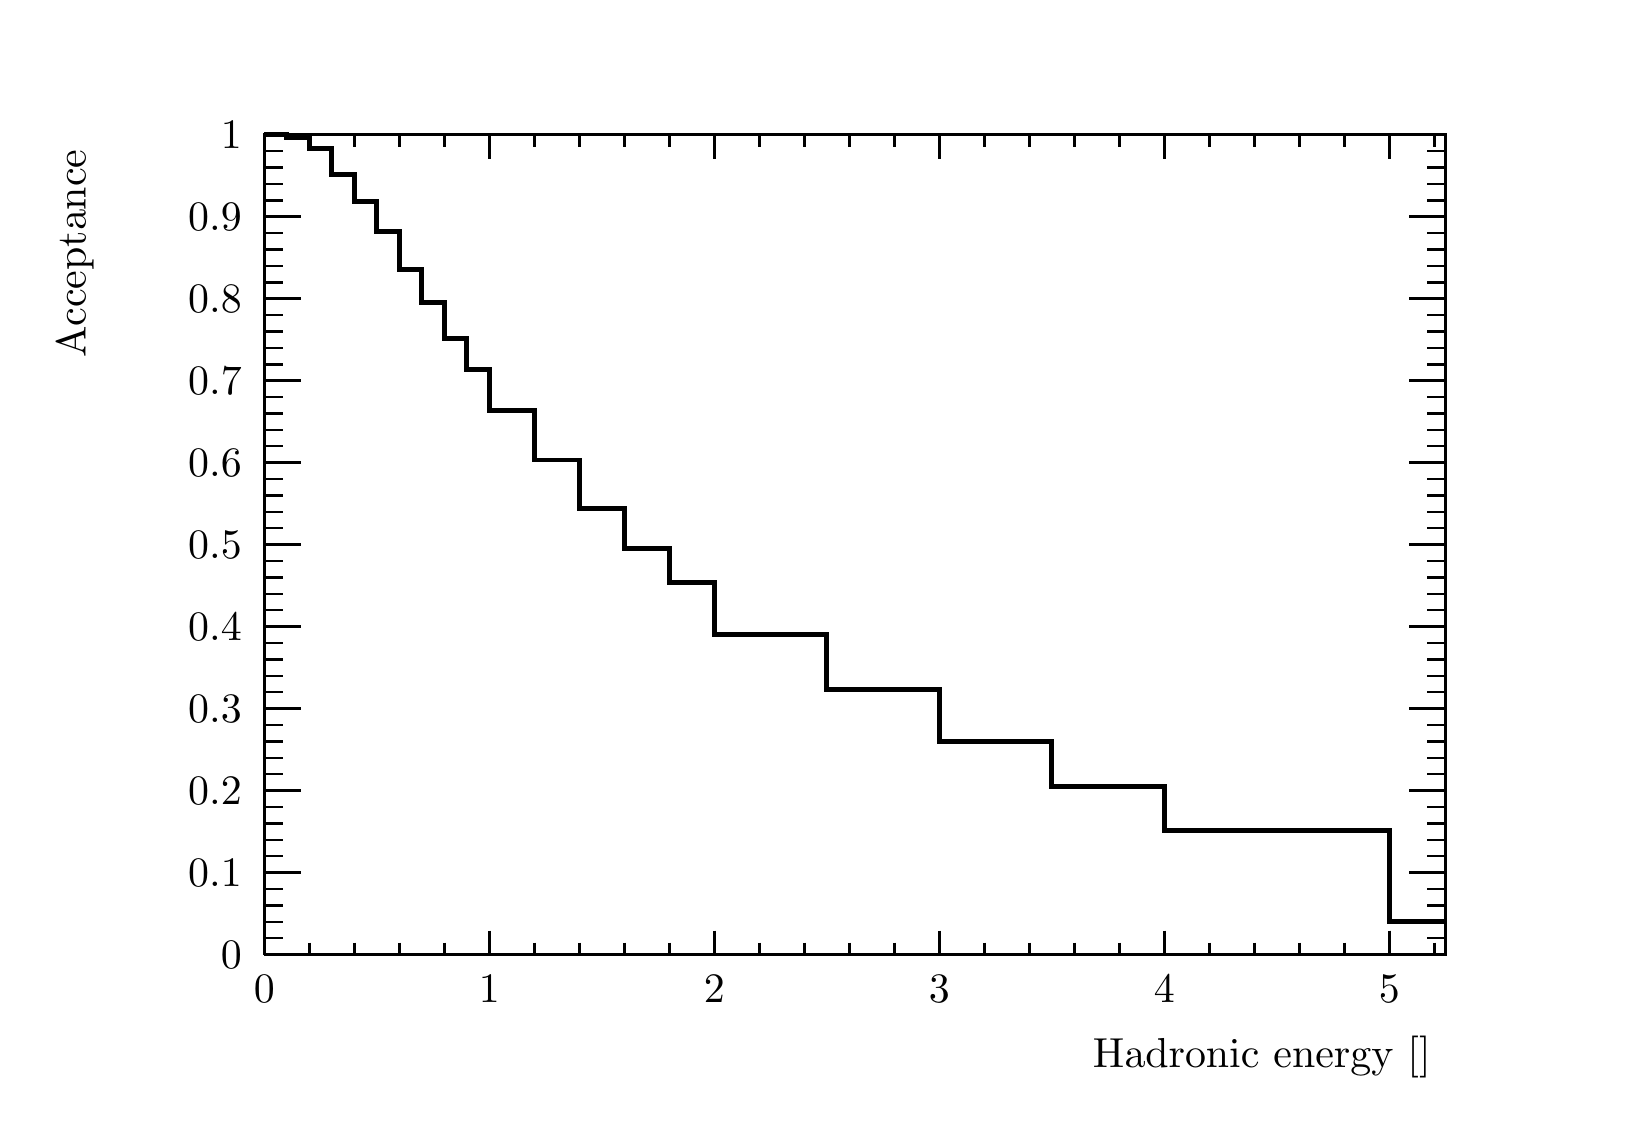
\begin{tikzpicture}
\pgfdeclareplotmark{cross} {
\pgfpathmoveto{\pgfpoint{-0.3\pgfplotmarksize}{\pgfplotmarksize}}
\pgfpathlineto{\pgfpoint{+0.3\pgfplotmarksize}{\pgfplotmarksize}}
\pgfpathlineto{\pgfpoint{+0.3\pgfplotmarksize}{0.3\pgfplotmarksize}}
\pgfpathlineto{\pgfpoint{+1\pgfplotmarksize}{0.3\pgfplotmarksize}}
\pgfpathlineto{\pgfpoint{+1\pgfplotmarksize}{-0.3\pgfplotmarksize}}
\pgfpathlineto{\pgfpoint{+0.3\pgfplotmarksize}{-0.3\pgfplotmarksize}}
\pgfpathlineto{\pgfpoint{+0.3\pgfplotmarksize}{-1.\pgfplotmarksize}}
\pgfpathlineto{\pgfpoint{-0.3\pgfplotmarksize}{-1.\pgfplotmarksize}}
\pgfpathlineto{\pgfpoint{-0.3\pgfplotmarksize}{-0.3\pgfplotmarksize}}
\pgfpathlineto{\pgfpoint{-1.\pgfplotmarksize}{-0.3\pgfplotmarksize}}
\pgfpathlineto{\pgfpoint{-1.\pgfplotmarksize}{0.3\pgfplotmarksize}}
\pgfpathlineto{\pgfpoint{-0.3\pgfplotmarksize}{0.3\pgfplotmarksize}}
\pgfpathclose
\pgfusepathqstroke
}
\pgfdeclareplotmark{cross*} {
\pgfpathmoveto{\pgfpoint{-0.3\pgfplotmarksize}{\pgfplotmarksize}}
\pgfpathlineto{\pgfpoint{+0.3\pgfplotmarksize}{\pgfplotmarksize}}
\pgfpathlineto{\pgfpoint{+0.3\pgfplotmarksize}{0.3\pgfplotmarksize}}
\pgfpathlineto{\pgfpoint{+1\pgfplotmarksize}{0.3\pgfplotmarksize}}
\pgfpathlineto{\pgfpoint{+1\pgfplotmarksize}{-0.3\pgfplotmarksize}}
\pgfpathlineto{\pgfpoint{+0.3\pgfplotmarksize}{-0.3\pgfplotmarksize}}
\pgfpathlineto{\pgfpoint{+0.3\pgfplotmarksize}{-1.\pgfplotmarksize}}
\pgfpathlineto{\pgfpoint{-0.3\pgfplotmarksize}{-1.\pgfplotmarksize}}
\pgfpathlineto{\pgfpoint{-0.3\pgfplotmarksize}{-0.3\pgfplotmarksize}}
\pgfpathlineto{\pgfpoint{-1.\pgfplotmarksize}{-0.3\pgfplotmarksize}}
\pgfpathlineto{\pgfpoint{-1.\pgfplotmarksize}{0.3\pgfplotmarksize}}
\pgfpathlineto{\pgfpoint{-0.3\pgfplotmarksize}{0.3\pgfplotmarksize}}
\pgfpathclose
\pgfusepathqfillstroke
}
\pgfdeclareplotmark{newstar} {
\pgfpathmoveto{\pgfqpoint{0pt}{\pgfplotmarksize}}
\pgfpathlineto{\pgfqpointpolar{44}{0.5\pgfplotmarksize}}
\pgfpathlineto{\pgfqpointpolar{18}{\pgfplotmarksize}}
\pgfpathlineto{\pgfqpointpolar{-20}{0.5\pgfplotmarksize}}
\pgfpathlineto{\pgfqpointpolar{-54}{\pgfplotmarksize}}
\pgfpathlineto{\pgfqpointpolar{-90}{0.5\pgfplotmarksize}}
\pgfpathlineto{\pgfqpointpolar{234}{\pgfplotmarksize}}
\pgfpathlineto{\pgfqpointpolar{198}{0.5\pgfplotmarksize}}
\pgfpathlineto{\pgfqpointpolar{162}{\pgfplotmarksize}}
\pgfpathlineto{\pgfqpointpolar{134}{0.5\pgfplotmarksize}}
\pgfpathclose
\pgfusepathqstroke
}
\pgfdeclareplotmark{newstar*} {
\pgfpathmoveto{\pgfqpoint{0pt}{\pgfplotmarksize}}
\pgfpathlineto{\pgfqpointpolar{44}{0.5\pgfplotmarksize}}
\pgfpathlineto{\pgfqpointpolar{18}{\pgfplotmarksize}}
\pgfpathlineto{\pgfqpointpolar{-20}{0.5\pgfplotmarksize}}
\pgfpathlineto{\pgfqpointpolar{-54}{\pgfplotmarksize}}
\pgfpathlineto{\pgfqpointpolar{-90}{0.5\pgfplotmarksize}}
\pgfpathlineto{\pgfqpointpolar{234}{\pgfplotmarksize}}
\pgfpathlineto{\pgfqpointpolar{198}{0.5\pgfplotmarksize}}
\pgfpathlineto{\pgfqpointpolar{162}{\pgfplotmarksize}}
\pgfpathlineto{\pgfqpointpolar{134}{0.5\pgfplotmarksize}}
\pgfpathclose
\pgfusepathqfillstroke
}
\definecolor{c}{rgb}{1,1,1};
\draw [color=c, fill=c] (0,0) rectangle (20,13.5227);
\draw [color=c, fill=c] (3,1.75795) rectangle (18,12.1705);
\definecolor{c}{rgb}{0,0,0};
\draw [c,line width=0.9] (3,1.75795) -- (3,12.1705) -- (18,12.1705) -- (18,1.75795) -- (3,1.75795);
\definecolor{c}{rgb}{1,1,1};
\draw [color=c, fill=c] (3,1.75795) rectangle (18,12.1705);
\definecolor{c}{rgb}{0,0,0};
\draw [c,line width=0.9] (3,1.75795) -- (3,12.1705) -- (18,12.1705) -- (18,1.75795) -- (3,1.75795);
\draw [c,line width=1.8] (3,12.1669) -- (3.28571,12.1669) -- (3.28571,12.1337) -- (3.57143,12.1337) -- (3.57143,11.9974) -- (3.85714,11.9974) -- (3.85714,11.6598) -- (4.14286,11.6598) -- (4.14286,11.3159) -- (4.42857,11.3159) -- (4.42857,10.9376) --
 (4.71429,10.9376) -- (4.71429,10.4567) -- (5,10.4567) -- (5,10.038) -- (5.28571,10.038) -- (5.28571,9.58251) -- (5.57143,9.58251) -- (5.57143,9.19266) -- (5.85714,9.19266) -- (5.85714,8.6728) -- (6.42857,8.6728) -- (6.42857,8.03916) -- (7,8.03916)
 -- (7,7.41873) -- (7.57143,7.41873) -- (7.57143,6.91137) -- (8.14286,6.91137) -- (8.14286,6.48146) -- (8.71429,6.48146) -- (8.71429,5.82387) -- (10.1429,5.82387) -- (10.1429,5.12498) -- (11.5714,5.12498) -- (11.5714,4.45809) -- (13,4.45809) --
 (13,3.88768) -- (14.4286,3.88768) -- (14.4286,3.33927) -- (17.2857,3.33927) -- (17.2857,2.18148) -- (18,2.18148);
\draw [c,line width=0.9] (3,1.75795) -- (18,1.75795);
\draw [c,line width=0.9] (3,2.06222) -- (3,1.75795);
\draw [c,line width=0.9] (3.57143,1.91009) -- (3.57143,1.75795);
\draw [c,line width=0.9] (4.14286,1.91009) -- (4.14286,1.75795);
\draw [c,line width=0.9] (4.71429,1.91009) -- (4.71429,1.75795);
\draw [c,line width=0.9] (5.28571,1.91009) -- (5.28571,1.75795);
\draw [c,line width=0.9] (5.85714,2.06222) -- (5.85714,1.75795);
\draw [c,line width=0.9] (6.42857,1.91009) -- (6.42857,1.75795);
\draw [c,line width=0.9] (7,1.91009) -- (7,1.75795);
\draw [c,line width=0.9] (7.57143,1.91009) -- (7.57143,1.75795);
\draw [c,line width=0.9] (8.14286,1.91009) -- (8.14286,1.75795);
\draw [c,line width=0.9] (8.71429,2.06222) -- (8.71429,1.75795);
\draw [c,line width=0.9] (9.28571,1.91009) -- (9.28571,1.75795);
\draw [c,line width=0.9] (9.85714,1.91009) -- (9.85714,1.75795);
\draw [c,line width=0.9] (10.4286,1.91009) -- (10.4286,1.75795);
\draw [c,line width=0.9] (11,1.91009) -- (11,1.75795);
\draw [c,line width=0.9] (11.5714,2.06222) -- (11.5714,1.75795);
\draw [c,line width=0.9] (12.1429,1.91009) -- (12.1429,1.75795);
\draw [c,line width=0.9] (12.7143,1.91009) -- (12.7143,1.75795);
\draw [c,line width=0.9] (13.2857,1.91009) -- (13.2857,1.75795);
\draw [c,line width=0.9] (13.8571,1.91009) -- (13.8571,1.75795);
\draw [c,line width=0.9] (14.4286,2.06222) -- (14.4286,1.75795);
\draw [c,line width=0.9] (15,1.91009) -- (15,1.75795);
\draw [c,line width=0.9] (15.5714,1.91009) -- (15.5714,1.75795);
\draw [c,line width=0.9] (16.1429,1.91009) -- (16.1429,1.75795);
\draw [c,line width=0.9] (16.7143,1.91009) -- (16.7143,1.75795);
\draw [c,line width=0.9] (17.2857,2.06222) -- (17.2857,1.75795);
\draw [c,line width=0.9] (17.2857,2.06222) -- (17.2857,1.75795);
\draw [c,line width=0.9] (17.8571,1.91009) -- (17.8571,1.75795);
\draw [anchor=base] (3,1.14943) node[scale=1.5143, color=c, rotate=0]{0};
\draw [anchor=base] (5.85714,1.14943) node[scale=1.5143, color=c, rotate=0]{1};
\draw [anchor=base] (8.71429,1.14943) node[scale=1.5143, color=c, rotate=0]{2};
\draw [anchor=base] (11.5714,1.14943) node[scale=1.5143, color=c, rotate=0]{3};
\draw [anchor=base] (14.4286,1.14943) node[scale=1.5143, color=c, rotate=0]{4};
\draw [anchor=base] (17.2857,1.14943) node[scale=1.5143, color=c, rotate=0]{5};
\draw [anchor= east] (18,0.459773) node[scale=1.5143, color=c, rotate=0]{Hadronic energy [\si{\GeV}] };
\draw [c,line width=0.9] (3,12.1705) -- (18,12.1705);
\draw [c,line width=0.9] (3,11.8662) -- (3,12.1705);
\draw [c,line width=0.9] (3.57143,12.0183) -- (3.57143,12.1705);
\draw [c,line width=0.9] (4.14286,12.0183) -- (4.14286,12.1705);
\draw [c,line width=0.9] (4.71429,12.0183) -- (4.71429,12.1705);
\draw [c,line width=0.9] (5.28571,12.0183) -- (5.28571,12.1705);
\draw [c,line width=0.9] (5.85714,11.8662) -- (5.85714,12.1705);
\draw [c,line width=0.9] (6.42857,12.0183) -- (6.42857,12.1705);
\draw [c,line width=0.9] (7,12.0183) -- (7,12.1705);
\draw [c,line width=0.9] (7.57143,12.0183) -- (7.57143,12.1705);
\draw [c,line width=0.9] (8.14286,12.0183) -- (8.14286,12.1705);
\draw [c,line width=0.9] (8.71429,11.8662) -- (8.71429,12.1705);
\draw [c,line width=0.9] (9.28571,12.0183) -- (9.28571,12.1705);
\draw [c,line width=0.9] (9.85714,12.0183) -- (9.85714,12.1705);
\draw [c,line width=0.9] (10.4286,12.0183) -- (10.4286,12.1705);
\draw [c,line width=0.9] (11,12.0183) -- (11,12.1705);
\draw [c,line width=0.9] (11.5714,11.8662) -- (11.5714,12.1705);
\draw [c,line width=0.9] (12.1429,12.0183) -- (12.1429,12.1705);
\draw [c,line width=0.9] (12.7143,12.0183) -- (12.7143,12.1705);
\draw [c,line width=0.9] (13.2857,12.0183) -- (13.2857,12.1705);
\draw [c,line width=0.9] (13.8571,12.0183) -- (13.8571,12.1705);
\draw [c,line width=0.9] (14.4286,11.8662) -- (14.4286,12.1705);
\draw [c,line width=0.9] (15,12.0183) -- (15,12.1705);
\draw [c,line width=0.9] (15.5714,12.0183) -- (15.5714,12.1705);
\draw [c,line width=0.9] (16.1429,12.0183) -- (16.1429,12.1705);
\draw [c,line width=0.9] (16.7143,12.0183) -- (16.7143,12.1705);
\draw [c,line width=0.9] (17.2857,11.8662) -- (17.2857,12.1705);
\draw [c,line width=0.9] (17.2857,11.8662) -- (17.2857,12.1705);
\draw [c,line width=0.9] (17.8571,12.0183) -- (17.8571,12.1705);
\draw [c,line width=0.9] (3,1.75795) -- (3,12.1705);
\draw [c,line width=0.9] (3.462,1.75795) -- (3,1.75795);
\draw [c,line width=0.9] (3.231,1.9662) -- (3,1.9662);
\draw [c,line width=0.9] (3.231,2.17445) -- (3,2.17445);
\draw [c,line width=0.9] (3.231,2.3827) -- (3,2.3827);
\draw [c,line width=0.9] (3.231,2.59095) -- (3,2.59095);
\draw [c,line width=0.9] (3.462,2.7992) -- (3,2.7992);
\draw [c,line width=0.9] (3.231,3.00745) -- (3,3.00745);
\draw [c,line width=0.9] (3.231,3.2157) -- (3,3.2157);
\draw [c,line width=0.9] (3.231,3.42395) -- (3,3.42395);
\draw [c,line width=0.9] (3.231,3.6322) -- (3,3.6322);
\draw [c,line width=0.9] (3.462,3.84045) -- (3,3.84045);
\draw [c,line width=0.9] (3.231,4.0487) -- (3,4.0487);
\draw [c,line width=0.9] (3.231,4.25695) -- (3,4.25695);
\draw [c,line width=0.9] (3.231,4.4652) -- (3,4.4652);
\draw [c,line width=0.9] (3.231,4.67345) -- (3,4.67345);
\draw [c,line width=0.9] (3.462,4.8817) -- (3,4.8817);
\draw [c,line width=0.9] (3.231,5.08995) -- (3,5.08995);
\draw [c,line width=0.9] (3.231,5.2982) -- (3,5.2982);
\draw [c,line width=0.9] (3.231,5.50645) -- (3,5.50645);
\draw [c,line width=0.9] (3.231,5.7147) -- (3,5.7147);
\draw [c,line width=0.9] (3.462,5.92295) -- (3,5.92295);
\draw [c,line width=0.9] (3.231,6.1312) -- (3,6.1312);
\draw [c,line width=0.9] (3.231,6.33945) -- (3,6.33945);
\draw [c,line width=0.9] (3.231,6.5477) -- (3,6.5477);
\draw [c,line width=0.9] (3.231,6.75595) -- (3,6.75595);
\draw [c,line width=0.9] (3.462,6.9642) -- (3,6.9642);
\draw [c,line width=0.9] (3.231,7.17245) -- (3,7.17245);
\draw [c,line width=0.9] (3.231,7.3807) -- (3,7.3807);
\draw [c,line width=0.9] (3.231,7.58895) -- (3,7.58895);
\draw [c,line width=0.9] (3.231,7.7972) -- (3,7.7972);
\draw [c,line width=0.9] (3.462,8.00545) -- (3,8.00545);
\draw [c,line width=0.9] (3.231,8.2137) -- (3,8.2137);
\draw [c,line width=0.9] (3.231,8.42195) -- (3,8.42195);
\draw [c,line width=0.9] (3.231,8.6302) -- (3,8.6302);
\draw [c,line width=0.9] (3.231,8.83845) -- (3,8.83845);
\draw [c,line width=0.9] (3.462,9.0467) -- (3,9.0467);
\draw [c,line width=0.9] (3.231,9.25495) -- (3,9.25495);
\draw [c,line width=0.9] (3.231,9.4632) -- (3,9.4632);
\draw [c,line width=0.9] (3.231,9.67145) -- (3,9.67145);
\draw [c,line width=0.9] (3.231,9.8797) -- (3,9.8797);
\draw [c,line width=0.9] (3.462,10.088) -- (3,10.088);
\draw [c,line width=0.9] (3.231,10.2962) -- (3,10.2962);
\draw [c,line width=0.9] (3.231,10.5045) -- (3,10.5045);
\draw [c,line width=0.9] (3.231,10.7127) -- (3,10.7127);
\draw [c,line width=0.9] (3.231,10.921) -- (3,10.921);
\draw [c,line width=0.9] (3.462,11.1292) -- (3,11.1292);
\draw [c,line width=0.9] (3.231,11.3375) -- (3,11.3375);
\draw [c,line width=0.9] (3.231,11.5457) -- (3,11.5457);
\draw [c,line width=0.9] (3.231,11.754) -- (3,11.754);
\draw [c,line width=0.9] (3.231,11.9622) -- (3,11.9622);
\draw [c,line width=0.9] (3.462,12.1705) -- (3,12.1705);
\draw [anchor= east] (2.9,1.75795) node[scale=1.5143, color=c, rotate=0]{0};
\draw [anchor= east] (2.9,2.7992) node[scale=1.5143, color=c, rotate=0]{0.1};
\draw [anchor= east] (2.9,3.84045) node[scale=1.5143, color=c, rotate=0]{0.2};
\draw [anchor= east] (2.9,4.8817) node[scale=1.5143, color=c, rotate=0]{0.3};
\draw [anchor= east] (2.9,5.92295) node[scale=1.5143, color=c, rotate=0]{0.4};
\draw [anchor= east] (2.9,6.9642) node[scale=1.5143, color=c, rotate=0]{0.5};
\draw [anchor= east] (2.9,8.00545) node[scale=1.5143, color=c, rotate=0]{0.6};
\draw [anchor= east] (2.9,9.0467) node[scale=1.5143, color=c, rotate=0]{0.7};
\draw [anchor= east] (2.9,10.088) node[scale=1.5143, color=c, rotate=0]{0.8};
\draw [anchor= east] (2.9,11.1292) node[scale=1.5143, color=c, rotate=0]{0.9};
\draw [anchor= east] (2.9,12.1705) node[scale=1.5143, color=c, rotate=0]{1};
\draw [anchor= east] (0.6,12.1705) node[scale=1.5143, color=c, rotate=90]{Acceptance};
\draw [c,line width=0.9] (18,1.75795) -- (18,12.1705);
\draw [c,line width=0.9] (17.538,1.75795) -- (18,1.75795);
\draw [c,line width=0.9] (17.769,1.9662) -- (18,1.9662);
\draw [c,line width=0.9] (17.769,2.17445) -- (18,2.17445);
\draw [c,line width=0.9] (17.769,2.3827) -- (18,2.3827);
\draw [c,line width=0.9] (17.769,2.59095) -- (18,2.59095);
\draw [c,line width=0.9] (17.538,2.7992) -- (18,2.7992);
\draw [c,line width=0.9] (17.769,3.00745) -- (18,3.00745);
\draw [c,line width=0.9] (17.769,3.2157) -- (18,3.2157);
\draw [c,line width=0.9] (17.769,3.42395) -- (18,3.42395);
\draw [c,line width=0.9] (17.769,3.6322) -- (18,3.6322);
\draw [c,line width=0.9] (17.538,3.84045) -- (18,3.84045);
\draw [c,line width=0.9] (17.769,4.0487) -- (18,4.0487);
\draw [c,line width=0.9] (17.769,4.25695) -- (18,4.25695);
\draw [c,line width=0.9] (17.769,4.4652) -- (18,4.4652);
\draw [c,line width=0.9] (17.769,4.67345) -- (18,4.67345);
\draw [c,line width=0.9] (17.538,4.8817) -- (18,4.8817);
\draw [c,line width=0.9] (17.769,5.08995) -- (18,5.08995);
\draw [c,line width=0.9] (17.769,5.2982) -- (18,5.2982);
\draw [c,line width=0.9] (17.769,5.50645) -- (18,5.50645);
\draw [c,line width=0.9] (17.769,5.7147) -- (18,5.7147);
\draw [c,line width=0.9] (17.538,5.92295) -- (18,5.92295);
\draw [c,line width=0.9] (17.769,6.1312) -- (18,6.1312);
\draw [c,line width=0.9] (17.769,6.33945) -- (18,6.33945);
\draw [c,line width=0.9] (17.769,6.5477) -- (18,6.5477);
\draw [c,line width=0.9] (17.769,6.75595) -- (18,6.75595);
\draw [c,line width=0.9] (17.538,6.9642) -- (18,6.9642);
\draw [c,line width=0.9] (17.769,7.17245) -- (18,7.17245);
\draw [c,line width=0.9] (17.769,7.3807) -- (18,7.3807);
\draw [c,line width=0.9] (17.769,7.58895) -- (18,7.58895);
\draw [c,line width=0.9] (17.769,7.7972) -- (18,7.7972);
\draw [c,line width=0.9] (17.538,8.00545) -- (18,8.00545);
\draw [c,line width=0.9] (17.769,8.2137) -- (18,8.2137);
\draw [c,line width=0.9] (17.769,8.42195) -- (18,8.42195);
\draw [c,line width=0.9] (17.769,8.6302) -- (18,8.6302);
\draw [c,line width=0.9] (17.769,8.83845) -- (18,8.83845);
\draw [c,line width=0.9] (17.538,9.0467) -- (18,9.0467);
\draw [c,line width=0.9] (17.769,9.25495) -- (18,9.25495);
\draw [c,line width=0.9] (17.769,9.4632) -- (18,9.4632);
\draw [c,line width=0.9] (17.769,9.67145) -- (18,9.67145);
\draw [c,line width=0.9] (17.769,9.8797) -- (18,9.8797);
\draw [c,line width=0.9] (17.538,10.088) -- (18,10.088);
\draw [c,line width=0.9] (17.769,10.2962) -- (18,10.2962);
\draw [c,line width=0.9] (17.769,10.5045) -- (18,10.5045);
\draw [c,line width=0.9] (17.769,10.7127) -- (18,10.7127);
\draw [c,line width=0.9] (17.769,10.921) -- (18,10.921);
\draw [c,line width=0.9] (17.538,11.1292) -- (18,11.1292);
\draw [c,line width=0.9] (17.769,11.3375) -- (18,11.3375);
\draw [c,line width=0.9] (17.769,11.5457) -- (18,11.5457);
\draw [c,line width=0.9] (17.769,11.754) -- (18,11.754);
\draw [c,line width=0.9] (17.769,11.9622) -- (18,11.9622);
\draw [c,line width=0.9] (17.538,12.1705) -- (18,12.1705);
\end{tikzpicture}

		\end{adjustbox}
	\end{minipage}
	\caption[Muonic and hadronic acceptance for CC neutrino interactions in ND-LAr]{Left: Muonic acceptance for CC muon neutrino interactions in ND-LAr as a function of transverse and longitudinal muon momentum. Right: Hadronic acceptance for CC muon neutrino interactions in ND-LAr as a function of true hadronic energy. Both from~\cite{Abi:2020qib}.}
	\label{fig:ndAcceptance}
\end{figure}

The uncertainty on the muon and hadron acceptance is produced from the respective plots in \citefig{fig:ndAcceptance} with a higher uncertainty in regions where the acceptance is rapidly changing and thus vulnerable to mismodelling.
